%%%%%%%%%%%%%%%%%%%%%%%%%%%%%%%%%%%%%%%%%%%%%%%%%%%%%%%%%%%%%%%
%% OXFORD THESIS TEMPLATE

% Use this template to produce a standard thesis that meets the Oxford University requirements for DPhil submission
%
% Originally by Keith A. Gillow (gillow@maths.ox.ac.uk), 1997
% Modified by Sam Evans (sam@samuelevansresearch.org), 2007
% Modified by John McManigle (john@oxfordechoes.com), 2015
%
% This version Copyright (c) 2015-2017 John McManigle
%
% Broad permissions are granted to use, modify, and distribute this software
% as specified in the MIT License included in this distribution's LICENSE file.
%

% I've (John) tried to comment this file extensively, so read through it to see how to use the various options.  Remember
% that in LaTeX, any line starting with a % is NOT executed.  Several places below, you have a choice of which line to use
% out of multiple options (eg draft vs final, for PDF vs for binding, etc.)  When you pick one, add a % to the beginning of
% the lines you don't want.

%%%%% CHOOSE PAGE LAYOUT
% The most common choices should be below.  You can also do other things, like replacing "a4paper" with "letterpaper", etc.

% This one will format for two-sided binding (ie left and right pages have mirror margins; blank pages inserted where needed):
\documentclass[a4paper,twoside]{ociamthesis}
% This one will format for one-sided binding (ie left margin > right margin; no extra blank pages):
%\documentclass[a4paper]{ociamthesis}
% This one will format for PDF output (ie equal margins, no extra blank pages):
%\documentclass[a4paper,nobind]{ociamthesis} 


%%%%% SELECT YOUR DRAFT OPTIONS
% Three options going on here; use in any combination.  But remember to turn the first two off before
% generating a PDF to send to the printer!

% This adds a "DRAFT" footer to every normal page.  (The first page of each chapter is not a "normal" page.)
%\fancyfoot[C]{\emph{DRAFT Printed on \today}}  

% This highlights (in blue) corrections marked with (for words) \mccorrect{blah} or (for whole
% paragraphs) \begin{mccorrection} . . . \end{mccorrection}.  This can be useful for sending a PDF of
% your corrected thesis to your examiners for review.  Turn it off, and the blue disappears.
%\correctionstrue


%%%%% BIBLIOGRAPHY SETUP
% Note that your bibliography will require some tweaking depending on your department, preferred format, etc.
% The options included below are just very basic "sciencey" and "humanitiesey" options to get started.
% If you've not used LaTeX before, I recommend reading a little about biblatex/biber and getting started with it.
% If you're already a LaTeX pro and are used to natbib or something, modify as necessary.
% Either way, you'll have to choose and configure an appropriate bibliography format...

% The science-type option: numerical in-text citation with references in order of appearance.
%\usepackage[style=numeric-comp, sorting=none, backend=biber, doi=false, isbn=false]{biblatex}
%\newcommand*{\bibtitle}{References}

% The humanities-type option: author-year in-text citation with an alphabetical works cited.
%\usepackage[style=authoryear, sorting=nyt, backend=biber, maxcitenames=2, useprefix, doi=false, isbn=false]{biblatex}
%\newcommand*{\bibtitle}{Works Cited}

% I-Jun reference style
% The humanities-type option: author-year in-text citation with an alphabetical works cited.
%\usepackage[backend=biber, style=authoryear, sorting=nyt, uniquename=init, maxcitenames=1, maxbibnames=6, minbibnames=6, giveninits=true, doi=false, url=false, isbn=false, uniquelist=false, sortcites=true]{biblatex}

\usepackage[backend=biber,style=apa, uniquename=false, uniquelist=false,  maxcitenames=1, url=false, sorting=nyt, sortcites=true]{biblatex}
\DeclareLanguageMapping{english}{english-apa}

% CGaddition
\setlength\bibitemsep{\baselineskip}
\renewbibmacro{in:}{}
\newcommand*{\bibtitle}{References}

% IJLaddition
\usepackage[T1]{fontenc}
\usepackage[utf8]{inputenc}
\usepackage{babel}
\usepackage{csquotes}
\DefineBibliographyStrings{english}{
  andothers = {\mkbibemph{et\addabbrvspace al\adddot}}
}

% JH addition

\usepackage{wrapfig} % single column figures
\usepackage{amsmath} % align math equations

\usepackage[compact]{titlesec} % adjust title before/after spacing
\titlespacing{\section}{0pt}{*4}{*0}
\titlespacing{\subsection}{0pt}{*1}{*0}
\titlespacing{\subsubsection}{0pt}{*1}{*0}

\usepackage{hyphenat}

\usepackage{rotating} % Rotate figures

%\usepackage{sectsty}
%\sectionfont{\raggedright}
%\chapterfont{\raggedright}
%\allsectionsfont{\raggedright}
%\chapterfont{\raggedright}

% Change font
% TO DO!!

% This makes the bibliography left-aligned (not 'justified') and slightly smaller font.
%\renewcommand*{\bibfont}{\raggedright\small}

% Change this to the name of your .bib file (usually exported from a citation manager like Zotero or EndNote).
\addbibresource{references.bib}


% Uncomment this if you want equation numbers per section (2.3.12), instead of per chapter (2.18):
%\numberwithin{equation}{subsection}


%%%%% Switch figures off (for drafting purposes)
%\usepackage[figuresonly,nolists,nomarkers]{endfloat}
%\renewcommand{\processdelayedfloats}{}


%%%%% THESIS / TITLE PAGE INFORMATION
% Everybody needs to complete the following:
%\title{Regulatory Networks and transcription \linebreak factor}
\title{Regulatory network analyses highlight transcription factor cooperation in haematopoiesis and leukaemogenesis}
%Analysis of GRNs that drive haemaopotrepoiwe and leukaemogenesis
\author{Joe Ritchie Harman}
\college{Hertford College}

% Master's candidates who require the alternate title page (with candidate number and word count)
% must also un-comment and complete the following three lines:
%\masterssubmissiontrue
%\candidateno{933516}
%\wordcount{28,815}

% Uncomment the following line if your degree also includes exams (eg most masters):
%\renewcommand{\submittedtext}{Submitted in partial completion of the}
% Your full degree name.  (But remember that DPhils aren't "in" anything.  They're just DPhils.)
\degree{Doctor of Philosophy}
% Term and year of submission, or date if your board requires (eg most masters)
\degreedate{Michaelmas 2022}


%%%%% YOUR OWN PERSONAL MACROS
% This is a good place to dump your own LaTeX macros as they come up.

\newcommand{\citep}{\parencite}

% this command defines italicised n
\newcommand{\n}{\textit{n}}

% this command defines degrees centigrade notation
\newcommand{\dc}{\textsuperscript{o}C}

% this command defines H20 with subscript
\newcommand{\water}{H\textsubscript{2}O}

% this command defines carbon dioxide with subscript
\newcommand{\cotwo}{CO\textsubscript{2} }

% this command defines microliter with mu greek letter
\newcommand{\microl}{$\mu$l}

% this command defines microliter with mu greek letter at end of sentence (can also use \ ALLOW spaces!!!)
\newcommand{\microlEnd}{$\mu$l}

% this command defines micromolar with mu greek letter
\newcommand{\microm}{$\mu$M}

% this command defines micromolar with mu greek letter (with no trailing space)
\newcommand{\micromEnd}{$\mu$M}

% this command defines microgram with mu greek letter
\newcommand{\microg}{$\mu$g}

% this command defines microgram per ml with mu greek letter
\newcommand{\microgperml}{$\mu$gmL\textsuperscript{-1}}

% this command defines x10^ with superscript
%\newcommand{\xten}[2] {#1$\times 10^{#2}$}
\newcommand{\xten}[2] {#1 x 10\textsuperscript{#2}}
% example
%\xten{1}{5}
% produces
% 1x10^5

% this command defines per ml for eg cells/ml but using ^-1 notation to look fancy
\newcommand{\perml}{mL\textsuperscript{-1}}

% this command defines microliter per ml with mu greek letter
\newcommand{\microlperml}{$\mu$LmL\textsuperscript{-1} }

% this command defines milligram per ml
\newcommand{\migperml}{mgmL\textsuperscript{-1}}

% this command defines nanogram per microliter
\newcommand{\ngpermicrol}{ng$\mu$L\textsuperscript{-1}}

% defines U/μl with greek mu, and superscript^-1
\newcommand{\upermicrol}{U$\mu$L\textsuperscript{-1}}

% superscript + and -
\newcommand{\upos}{\textsuperscript{+}}
\newcommand{\uneg}{\textsuperscript{-}}

% Shorthand
\newcommand{\runxnull}{\textit{Runx1}\textsuperscript{-/-}}

\newcommand{\mybwt}{\textit{Myb}\textsuperscript{+/+}}

\newcommand{\mybmre}{\textit{Myb}\textsuperscript{MRE/MRE}}


% To make text superscripts shortcuts
	\renewcommand{\th}{\textsuperscript{th}} % ex: I won 4\th place
	\newcommand{\nd}{\textsuperscript{nd}}
	\renewcommand{\st}{\textsuperscript{st}}
	\newcommand{\rd}{\textsuperscript{rd}}

%CGaddition
    \makeatletter
    \renewcommand{\@makechapterhead}[1]{\chapterheadstartvskip%
      {\size@chapter{\sectfont
          {\chapnumfont
          \ifnum \c@secnumdepth >\m@ne%
            \if@mainmatter\noindent\thechapter%
            \fi\fi
            \par\nobreak}%
          {\interlinepenalty\@M\noindent #1\par}
        }
        \nobreak\chapterheadendvskip}}
    \makeatother

%CGaddition
    \usepackage{graphicx}
    \graphicspath{ {./figures/} }
    \usepackage{booktabs}
    \usepackage{tabularx}
    \usepackage{longtable}
    \usepackage{lscape}
    \usepackage{flafter}

%CGaddition
    \renewcommand{\chapterheadstartvskip}{\vspace*{-50pt}}

%IJLaddition
    \usepackage{textgreek}
    \usepackage{float}
    \usepackage{sidecap}
    \usepackage{hyperref}
    \usepackage{array}
    \usepackage[flushleft]{threeparttable}
    
    \usepackage{booktabs}

%%%%% THE ACTUAL DOCUMENT STARTS HERE
\begin{document}

% Fix spacing. Pick sloppy or set emergencystretch if needed.
\sloppy
%\emergencystretch

%%%%% CHOOSE YOUR LINE SPACING HERE
% This is the official option.  Use it for your submission copy and library copy:
\setlength{\textbaselineskip}{22pt plus2pt}
% This is closer spacing (about 1.5-spaced) that you might prefer for your personal copies:
%\setlength{\textbaselineskip}{18pt plus2pt minus1pt}

% You can set the spacing here for the roman-numbered pages (acknowledgements, table of contents, etc.)
\setlength{\frontmatterbaselineskip}{17pt plus1pt minus1pt}

% Leave this line alone; it gets things started for the real document.
\setlength{\baselineskip}{\textbaselineskip}


%%%%% CHOOSE YOUR SECTION NUMBERING DEPTH HERE
% You have two choices.  First, how far down are sections numbered?  (Below that, they're named but
% don't get numbers.)  Second, what level of section appears in the table of contents?  These don't have
% to match: you can have numbered sections that don't show up in the ToC, or unnumbered sections that
% do.  Throughout, 0 = chapter; 1 = section; 2 = subsection; 3 = subsubsection, 4 = paragraph...

% The level that gets a number:
\setcounter{secnumdepth}{3}
% The level that shows up in the ToC:
\setcounter{tocdepth}{2}


%%%%% ABSTRACT SEPARATE
% This is used to create the separate, one-page abstract that you are required to hand into the Exam
% Schools.  You can comment it out to generate a PDF for printing or whatnot.
%\begin{abstractseparate}
%	
The regulation of gene expression is a complex process that confers cell identity and drives cell differentiation. Transcription factors (TFs) are an important modulator of gene expression and are critical to understanding the regulatory code characterising cell behaviour. However, TFs function in cooperation with one another, acting as a complex combinatorial code to enact gene regulation. Gene regulatory network (GRN) models are used to describe the regulation of genes and to account for this combinatorial code. When the regulatory code underpinning normal cell behaviour goes awry this can lead to abnormal GRNs and the development of disease. This poses two questions: how does TF cooperation drive cellular processes, and how are normal GRNs deregulated in disease?

Haematopoietic stem cells are first established in the developing embryo through a process known as the endothelial-to-haematopoietic transition (EHT). EHT involves dynamic gene regulation across well-defined populations, and is critically dependent on the master TF regulator, RUNX1. EHT is therefore a fascinating system to study TF regulation in driving a complex developmental process. When haematopoietic GRNs are misregulated this can lead to disease. A common childhood leukaemia involves chromosomal rearrangements resulting in novel Mixed Lineage Leukaemia (MLL) fusion proteins that aberrantly drive transcription. MLL-rearranged leukaemias are considered a wholly transcriptional disease, and as such are uniquely suited for studying through GRN approaches.

In this thesis, the study of GRNs underpinning normal and malignant haematopoietic processes revealed insights into the role of TF cooperation. Notably, Runx1 cooperates with TFs to drive repression of a transiently activated network during EHT. In MLL-AF4 leukaemia, MLL-AF4 drives TF cooperation by altering the chromatin environment and encouraging local TF binding, and within this MLL-AF4 context RUNX1 activity is biased towards activation. RUNX1 was also found to cooperate with MYB to synergistically activate \textit{BCL2} and \textit{MYC}, promoting leukaemogenesis. % Create an abstract.tex file in the 'text' folder for your abstract.
%\end{abstractseparate}


% JEM: Pages are roman numbered from here, though page numbers are invisible until ToC.  This is in
% keeping with most typesetting conventions.
\begin{romanpages}

% Title page is created here
\maketitle

%%%%% ACKNOWLEDGEMENTS -- Nothing to do here except comment out if you don't want it.
\begin{acknowledgements}
 	
%I have many people to thank who have advised and supported me, and without them I could not have written this thesis. I am very much a product of the people around me, and every one of my friends, colleagues, and academic advisors have shaped me as a scientist and I cannot thank them enough.

First and foremost, I would like to thank Prof. Tom Milne and Prof. Marella de Bruijn for being fantastic and supportive mentors. Working in Marella's lab gave me my first taste of academia, and helped me develop the critical groundwork for being an academic scientist. Tom has been an incredible guide in navigating my DPhil project, and has always pushed me to be imaginative and driven in my work. 
\vspace{-8pt}

The Milne lab has been home to many lovely colleagues, and I am grateful to work alongside all of them. Nick Crump has taught me many techniques and pushed my critical thinking. I will always remember the late-night lab chats, and spurious analysis sessions. I-Jun Lau has been kind and supportive, and always ready to talk science. To Nick and I-Jun: I'll never stop singing "do you like tdTomato". Alastair Smith has been good to talk to (and complain to) about coding, though I won't stop defending R over Python. Vassi Sharlandjieva, Nicole Jackson and Catherine Chahrour have been bright personalities in the lab, and have brought a little life back into work-life balance. Ross Thorne left the lab before I joined, but his initial work on networks was critical to my thesis, and his viva presentation was immensely inspirational. Outside the lab, Siobhan Rice and Simona Valletta were a fantastic help with mouse experiments.
\vspace{-8pt}

In the de Bruijn lab, Vincent Frontera was always entertaining to work with, and taught me a lot about flow cytometry. I'm thankful for Christina Rode, who patiently taught me many basic lab techniques, and was always a positive personality. Dominic Owens was a great colleague, who helped me with his CRISPR and capture-C knowledge, and always had a great story to tell. Emanuele Azzoni taught me how to perform whole mount imaging, which are not only scientifically useful, but are artistically beautiful. Lucas Greder performed experiments that have been the seed for my network analyses. Giorgio Anselmi and Alessandro Cavallo have always been ready and willing to talk science, particularly single cell analyses, and have offered great insight. Matt Nicholls has been meticulous in organising the lab, and I am grateful for the times he has kept me company in the mouse facility. Naeema Mehmood has been lovely to talk to - and I appreciate being able to talk about the latest Marvel films!
\vspace{-8pt}

Most importantly, I would like to thank my family. My mum, Angela, pushed me from a young age to do well academically. I'm sure I can only do maths because we recited the times table so often! My dad, Ritchie, has always supported me, and I inherited my love of fancy tech from him. My sister (the "cooler" sibling), Rachael, has been consistently supportive.% Finally, Claire has been incredibly supportive and patient while I've written this thesis!
\end{acknowledgements}

%%%%% DECLARATION -- Nothing to do here except comment out if you don't want it.
\begin{declaration}
 	I declare that the work presented in this thesis is my own unless otherwise stated, for example where my analyses used data from published work or data from collaborators. This thesis has not been submitted, either partially or in full, for another qualification of this University, or for a qualification at any other institution. 

\noindent
Much of the work in chapter 4 has been published in \cite{harman_kmt2a-aff1_2021}. I wrote the manuscript, analysed the data, and performed experiments in this publication and I declare that no work performed solely by others has been included, unless otherwise stated.

\noindent
\textbf{Collaborators and their contributions to this work:}

\noindent
For computational analyses presented in Chapters 3 and 4, I used experimental data generated by previous/current members of the de Bruijn and Milne labs, alongside published datasets. The sources of experimental data are indicated in the figure legends and in the main body of text. Unpublished data was sourced as follows:

\noindent
\textbf{Fig. \ref{fig:ch3_overview}} Unpublished mini-bulk RNA-seq and ATAC-seq data on cells undergoing EHT in the mouse embryo (de Bruijn group, L. Greder and G. Swiers) was used where I generated and explored an integrated network model of EHT.

\noindent
\textbf{Fig. \ref{fig:ch3_runx1-regulation}} Published tiled capture-C \citep{owens_dynamic_2022} was used to complement and extend the integrated EHT network model.

\noindent
\textbf{Fig. \ref{fig:ch3_runx1-ikzf1}} Unpublished Capture-C and qRT-PCR data (de Bruijn group, D. Owens and L. Greder) was used to complement findings from the EHT network.

\noindent
\textbf{Fig. \ref{fig:ch4_GRN_just}} Analysis performed by R. Thorne was included to introduce the hypothesis for chapter 4.

\noindent
\textbf{Fig. \ref{fig:ch4_peak-qc}} Unpublished MLL-N ChIP-seq data from patient samples (Milne group, N. Crump) was analysed and included to validate ChIP-seq peak calling.

\noindent
\textbf{Fig. \ref{fig:ch4_runx1-grn}} Unpublished nascent RNA-seq data following \textit{RUNX1} knockdown (Milne lab, M. Tapia) was used to generate a network model of RUNX1 in MLL-AF4 leukaemia.

\noindent
\textbf{Fig. \ref{fig:ch4_essentiality}} Analysis performed by T. Wilson on a published CRISPR essentiality screen (DepMap, Avana 21Q1, \cite{meyers_computational_2017, doench_optimized_2016}), under my supervision.

\noindent
\textbf{Fig. \ref{fig:ch4_multiome-clusters}, \ref{fig:ch4_multiome-erg}, \ref{fig:ch4_multiome-grn}, \ref{fig:ch4_multiome-tradeseq}} Single cell multiome data were generated in a collaboration between the Milne and Roy labs, involving myself, A. Smith, N. Elliott, and S. Rice. Data analysis was done by A. Smith and me: A. Smith contributed the pre-processing and quality control filtering of the ATAC-seq data. The rest of the analysis was performed by me.

\noindent
\textbf{Fig. \ref{fig:ch5_overview}} Mouse experiments (GMP isolation) were performed with assistance fom S. Valletta and S. Rice. The MLL-AF9 mCherry retroviral construct and \mybmre{} mouse models used in these experiments was designed and generated by I. Lau (Milne group).


\end{declaration}

%%%%% LIST OF PUBLICATIONS -- Nothing to do here except comment out if you don't want it.
\begin{publications}
 	\textit{Joint first authors indicated with *}

\noindent
\textbf{Harman JR}*, Thorne R*, Jamilly M, Tapia M, Crump NT, Rice S, Beveridge R, Morrissey E, de Bruijn MFTR, Roberts I, Roy A, Fulga TA, Milne TA. A KMT2A-AFF1 gene regulatory network highlights the role of core transcription factors and reveals the regulatory logic of key downstream target genes. Genome Res. 2021 Jun 4;31(7):1159–73

\noindent
\textbf{Harman JR}*, Greder L*, Swiers G, Owens DDG, Suciu M, Downes D, Telenius J, Frontera V, Antoniou S, Repapi E, Azzoni E, de Bruijn MFTR. A gene regulatory network of the endothelial-to-hematopoietic transition reveals a Runx1:Ikzf1:Notch feed-forward loop. \textit{Manuscript in preparation}.

\noindent
Fidyt K, Pastorczak A, Cyran J, Crump NT, Goral A, Madzio J, Muchowicz A, Poprzeczko M, Domka K, Komorowski L, Winiarska M, \textbf{Harman JR}, Siudakowska K, Graczyk-Jarzynka A, Patkowska E, Lech-Maranda E, Mlynarski W, Golab J, Milne TA, Firczuk M. Potent, p53-independent induction of NOXA sensitizes MLL-rearranged B-cell acute lymphoblastic leukemia cells to venetoclax. Oncogene. 2022 Mar;41(11):1600-1609

\noindent
Owens DDG, Anselmi G, Oudelaar AM, Downes DJ, Cavallo A, \textbf{Harman JR}, Schwessinger R, Bucakci A, Greder L, de Ornellas S, Jeziorska D, Telenius J, Hughes JR, de Bruijn MFTR. Dynamic Runx1 chromatin boundaries affect gene expression in hematopoietic development. Nat Commun. 2022 Feb 9;13(1):773

\noindent
Azzoni E, Frontera V, Anselmi G, Rode C, James C, Deltcheva EM, Demian AS, Brown J, Barone C, Patelli A, \textbf{Harman JR}, Nicholls M, Conway SJ, Morrissey E, Jacobsen SEW, Sparrow DB, Harris AL, Enver T, de Bruijn MFTR. The onset of circulation triggers a metabolic switch required for endothelial to hematopoietic transition. Cell Rep. 2021 Dec 14;37(11):110103

\noindent
Godfrey L, Crump NT, O'Byrne S, Lau IJ, Rice S, \textbf{Harman JR}, Jackson T, Elliott N, Buck G, Connor C, Thorne R, Knapp DJHF, Heidenreich O, Vyas P, Menendez P, Inglott S, Ancliff P, Geng H, Roberts I, Roy A, Milne TA. H3K79me2/3 controls enhancer-promoter interactions and activation of the pan-cancer stem cell marker PROM1/CD133 in MLL-AF4 leukemia cells. Leukemia. 2021 Jan;35(1):90-106

\noindent
Owens DDG, Caulder A, Frontera V, \textbf{Harman JR}, Allan AJ, Bucakci A, Greder L, Codner GF, Hublitz P, McHugh PJ, Teboul L, de Bruijn MFTR. Microhomologies are prevalent at Cas9-induced larger deletions. Nucleic Acids Res. 2019 Aug 22;47(14):7402-7417

\noindent
Godfrey L, Crump NT, Thorne R, Lau IJ, Repapi E, Dimou D, Smith AL, \textbf{Harman JR}, Telenius JM, Oudelaar A, Downes DJ, Vyas P, Hughes JR, Milne TA. DOT1L inhibition reveals a distinct subset of enhancers dependent on H3K79 methylation. Nature Communications. 10, 2803 (2019).

\noindent
\textbf{Conference attendance}

\noindent
Presentation: “Reconstruction of an EHT gene regulatory network identifies a Runx1:Ikzf1:Notch feed-forward loop”, International Society for Experimental Hematology. Online, August 2021.

\noindent
Poster: “RUNX1 gene regulatory network in leukaemia”, International RUNX conference. Seoul National University, Seoul, Korea. June 2019.

\end{publications}

% Bringing ToCs forward

\dominitoc % include a mini table of contents
\flushbottom

\begingroup
\raggedright
\tableofcontents
\endgroup

\listoffigures
	\mtcaddchapter
	
\listoftables
	\mtcaddchapter
	
% First parameter can be changed eg to "Glossary" or something.
% Second parameter is the max length of bold terms.
\begin{mclistof}{List of Abbreviations}{3.8cm}

\item[23GFP] +23 \textit{Runx1} enhancer GFP reporter

\item[AGM] Aorta-Gonad-Mesonephros

\item[ALL] Acute Lymphoblastic Leukaemia

\item[AML] Acute Myeloid Leukemia

\item[ATAC] Assay for Transposase-Accessible Chromatin

\item[bZIP] basic region leucine zipper

\item[chALL] Childhood ALL

\item[ChIP] Chromatin ImmunoPrecipitation

\item[CPM] Counts Per Million

\item[CTG] CellTiter-Glo (CTG)

\item[DAE] Differentially Accessible Element

\item[DBD] DNA Binding Domain

\item[DEG] Differentially Expressed Gene

\item[DOT1L] Disruptor Of Telomeric Silencing 1-Like

\item[EC] Endothelial Cell

\item[EHT] Endothelial-to-Haematopoietic Transition

\item[E-P] Enhancer-Promoter association

\item[EMT] Epithelial-to-Mesenchyme Transition

\item[FBM] Fetal Bone Marrow

\item[FC] Fold Change

\item[FCS] Fetal Calf Serum

\item[FFL] Feed-Forward Loop

\item[FL] Fetal Liver

\item[GCN] Gene Co-expression Network

\item[GMP] Granulocyte-Monocyte Progenitor

\item[GRN] Gene Regulatory Network

\item[HE] Haemogenic Endothelium

\item[HDAC] Histone DeAcetylase Complex

\item[HPC] Haematopoietic Progenitor Cell

\item[HSC] Haematopoietic Stem Cell

\item[HSPC] Haematopoietic Stem and Progenitor Cell

\item[IAC] Intra-Aortic Cluster

\item[iALL] Infant ALL

\item[KD] Knock-Down

\item[LMPP] Lympho-Myelo Primed Progenitors

\item[mESC] mouse Embryonic Stem Cells

\item[MLL] Mixed-Lineage Leukaemia

\item[\textit{MLL}r] \textit{MLL}-rearranged

\item[MLL-FP] MLL Fusion Protein

\item[MRE] miRNA Response Element

\item[NT] Non-Targeting

\item[PAS] Para-Aortic Splanchnopleura

\item[PCA] Principal Component Analysis

\item[Pol II] RNA Polymerase II

\item[PWM] Position Weight Matrix

\item[sc-multiome] Single cell RNA+ATAC multiome

\item[SEC] Super Elongation Complex (SEC)

\item[TAD] Topologically associated domain

\item[TF] Transcription Factor

\item[TPM] Transcripts Per Million

\item[TSS] Transcription Start Site

\item[uCpG] Unmethylated CpG

\item[UMAP] Uniform Manifold Approximation and Projection

\item[VU] Vitelline and Umbilical

\item[WNN] Weighted Nearest Neighbour

\item[wt-MLL] wild type MLL


\end{mclistof} 



% First parameter can be changed eg to "Glossary" or something.
% Second parameter is the max length of bold terms.
%\begin{mclistof}{List of terminology definitions}{5.5cm}
\begin{mclistof}{List of terminology definitions}{1cm}

\item[Bound gene] \hfill \\ A gene is considered bound if a ChIP-seq peak for a TF is found annotated to the nearest expressed promoter.

\item[Co-interaction] \hfill \\  Cases where two TFs commonly regulate the same enhancer or promoter regions in a GRN model. This definition does not imply cooperation.

\item[Definitive haematopoiesis] \hfill \\  The usage in this thesis refers to the generation of haematopoietic progenitors that persist in adult life, originating from either the yolk sac or the AGM. Historically, the yolk sac has previously been considered the site of primitive haematopoiesis. 

\item[Degree centrality] \hfill \\  Network statistic. The total number of edges connecting to an individual node (gene/protein).

\item[Edge] \hfill \\  Connection within a network. Two nodes are connected by an edge, which can be directional. Represented in this thesis as arrows, where the arrow point indicates the direction, such as TF regulation directed to a gene target.

\item[MLL-N/AF4-C] \hfill \\  When referring to MLL-N or AF4-C in ChIP-seq experiments, this refers to antibodies generated recognising the N or C terminus of the protein. MLL-N antibodies will bind to both wt-MLL and MLL-AF4. This project assumes MLL-N binding profiles reflect MLL-AF4 binding, as the majority of the DNA association domains are retained on the N-terminus portion of MLL. Robust MLL-AF4 peak calls were determined by MLL-N and AF4-C overlaps.

\item[Network motif] \hfill \\  The usage of the term "network" or "GRN" motif (as opposed to TF binding motif) refers to FFL and cascade motifs. These being specific 3-node network configurations that commonly occur as sub-structures in networks.

\item[Node] \hfill \\  Unit of a network. In this thesis this is used to refer to genes and their protein products interchangeably, depending on whether they are regulating (TF proteins) or targets (genes).

\item[Stress and betweenness centrality] \hfill \\  Similar network statistics that quantify how often a node is on a shortest path between other nodes of the network. Shortest paths are calculated between all possible pairs of nodes. Stress and betweenness are measures of how frequently an individual node is part of a shortest path. Stress is a quantification of shortest paths, while betweenness is represented as the proportion of all shortest paths in the network that pass through the node in question. As such, these measures can be thought to measure "bottle-necks" between two network regions.

\item[TF binding motif] \hfill \\  The usage of the term TF (DNA) binding motif (as opposed to network motif) refers to DNA sequences that particular TFs have an affinity to bind to. 

\end{mclistof} 


% TF motifs and GRN motifs

%%%%% DEDICATION -- If you'd like one, un-comment the following.
%\begin{dedication}
%This thesis is dedicated to\\
%someone\\
%for some special reason\\
%\end{dedication}


%%%%% ABSTRACT -- Nothing to do here except comment out if you don't want it.
\begin{abstract}
	\addcontentsline{toc}{chapter}{Abstract}
	
The regulation of gene expression is a complex process that confers cell identity and drives cell differentiation. Transcription factors (TFs) are an important modulator of gene expression and are critical to understanding the regulatory code characterising cell behaviour. However, TFs function in cooperation with one another, acting as a complex combinatorial code to enact gene regulation. Gene regulatory network (GRN) models are used to describe the regulation of genes and to account for this combinatorial code. When the regulatory code underpinning normal cell behaviour goes awry this can lead to abnormal GRNs and the development of disease. This poses two questions: how does TF cooperation drive cellular processes, and how are normal GRNs deregulated in disease?

Haematopoietic stem cells are first established in the developing embryo through a process known as the endothelial-to-haematopoietic transition (EHT). EHT involves dynamic gene regulation across well-defined populations, and is critically dependent on the master TF regulator, RUNX1. EHT is therefore a fascinating system to study TF regulation in driving a complex developmental process. When haematopoietic GRNs are misregulated this can lead to disease. A common childhood leukaemia involves chromosomal rearrangements resulting in novel Mixed Lineage Leukaemia (MLL) fusion proteins that aberrantly drive transcription. MLL-rearranged leukaemias are considered a wholly transcriptional disease, and as such are uniquely suited for studying through GRN approaches.

In this thesis, the study of GRNs underpinning normal and malignant haematopoietic processes revealed insights into the role of TF cooperation. Notably, Runx1 cooperates with TFs to drive repression of a transiently activated network during EHT. In MLL-AF4 leukaemia, MLL-AF4 drives TF cooperation by altering the chromatin environment and encouraging local TF binding, and within this MLL-AF4 context RUNX1 activity is biased towards activation. RUNX1 was also found to cooperate with MYB to synergistically activate \textit{BCL2} and \textit{MYC}, promoting leukaemogenesis.
\end{abstract}
\adjustmtc % Req. to fix minitoc ordering glitch


%%%%% MINI TABLES
% This lays the groundwork for per-chapter, mini tables of contents.  Comment the following line
% (and remove \minitoc from the chapter files) if you don't want this.  Un-comment either of the
% next two lines if you want a per-chapter list of figures or tables.
%\dominitoc % include a mini table of contents
%\dominilof  % include a mini list of figures
%\dominilot  % include a mini list of tables

% This aligns the bottom of the text of each page.  It generally makes things look better.
%\flushbottom

% This is where the whole-document ToC appears:
%\begingroup
%\raggedright
%\tableofcontents
%\endgroup


%\listoffigures
%	\mtcaddchapter
% \mtcaddchapter is needed when adding a non-chapter (but chapter-like) entity to avoid confusing minitoc

% Uncomment to generate a list of tables:
%\listoftables
%	\mtcaddchapter

%%%%% LIST OF ABBREVIATIONS
% This example includes a list of abbreviations.  Look at text/abbreviations.tex to see how that file is
% formatted.  The template can handle any kind of list though, so this might be a good place for a
% glossary, etc.
%% First parameter can be changed eg to "Glossary" or something.
% Second parameter is the max length of bold terms.
\begin{mclistof}{List of Abbreviations}{3.8cm}

\item[23GFP] +23 \textit{Runx1} enhancer GFP reporter

\item[AGM] Aorta-Gonad-Mesonephros

\item[ALL] Acute Lymphoblastic Leukaemia

\item[AML] Acute Myeloid Leukemia

\item[ATAC] Assay for Transposase-Accessible Chromatin

\item[bZIP] basic region leucine zipper

\item[chALL] Childhood ALL

\item[ChIP] Chromatin ImmunoPrecipitation

\item[CPM] Counts Per Million

\item[CTG] CellTiter-Glo (CTG)

\item[DAE] Differentially Accessible Element

\item[DBD] DNA Binding Domain

\item[DEG] Differentially Expressed Gene

\item[DOT1L] Disruptor Of Telomeric Silencing 1-Like

\item[EC] Endothelial Cell

\item[EHT] Endothelial-to-Haematopoietic Transition

\item[E-P] Enhancer-Promoter association

\item[EMT] Epithelial-to-Mesenchyme Transition

\item[FBM] Fetal Bone Marrow

\item[FC] Fold Change

\item[FCS] Fetal Calf Serum

\item[FFL] Feed-Forward Loop

\item[FL] Fetal Liver

\item[GCN] Gene Co-expression Network

\item[GMP] Granulocyte-Monocyte Progenitor

\item[GRN] Gene Regulatory Network

\item[HE] Haemogenic Endothelium

\item[HDAC] Histone DeAcetylase Complex

\item[HPC] Haematopoietic Progenitor Cell

\item[HSC] Haematopoietic Stem Cell

\item[HSPC] Haematopoietic Stem and Progenitor Cell

\item[IAC] Intra-Aortic Cluster

\item[iALL] Infant ALL

\item[KD] Knock-Down

\item[LMPP] Lympho-Myelo Primed Progenitors

\item[mESC] mouse Embryonic Stem Cells

\item[MLL] Mixed-Lineage Leukaemia

\item[\textit{MLL}r] \textit{MLL}-rearranged

\item[MLL-FP] MLL Fusion Protein

\item[MRE] miRNA Response Element

\item[NT] Non-Targeting

\item[PAS] Para-Aortic Splanchnopleura

\item[PCA] Principal Component Analysis

\item[Pol II] RNA Polymerase II

\item[PWM] Position Weight Matrix

\item[sc-multiome] Single cell RNA+ATAC multiome

\item[SEC] Super Elongation Complex (SEC)

\item[TAD] Topologically associated domain

\item[TF] Transcription Factor

\item[TPM] Transcripts Per Million

\item[TSS] Transcription Start Site

\item[uCpG] Unmethylated CpG

\item[UMAP] Uniform Manifold Approximation and Projection

\item[VU] Vitelline and Umbilical

\item[WNN] Weighted Nearest Neighbour

\item[wt-MLL] wild type MLL


\end{mclistof} 



%% First parameter can be changed eg to "Glossary" or something.
% Second parameter is the max length of bold terms.
%\begin{mclistof}{List of terminology definitions}{5.5cm}
\begin{mclistof}{List of terminology definitions}{1cm}

\item[Bound gene] \hfill \\ A gene is considered bound if a ChIP-seq peak for a TF is found annotated to the nearest expressed promoter.

\item[Co-interaction] \hfill \\  Cases where two TFs commonly regulate the same enhancer or promoter regions in a GRN model. This definition does not imply cooperation.

\item[Definitive haematopoiesis] \hfill \\  The usage in this thesis refers to the generation of haematopoietic progenitors that persist in adult life, originating from either the yolk sac or the AGM. Historically, the yolk sac has previously been considered the site of primitive haematopoiesis. 

\item[Degree centrality] \hfill \\  Network statistic. The total number of edges connecting to an individual node (gene/protein).

\item[Edge] \hfill \\  Connection within a network. Two nodes are connected by an edge, which can be directional. Represented in this thesis as arrows, where the arrow point indicates the direction, such as TF regulation directed to a gene target.

\item[MLL-N/AF4-C] \hfill \\  When referring to MLL-N or AF4-C in ChIP-seq experiments, this refers to antibodies generated recognising the N or C terminus of the protein. MLL-N antibodies will bind to both wt-MLL and MLL-AF4. This project assumes MLL-N binding profiles reflect MLL-AF4 binding, as the majority of the DNA association domains are retained on the N-terminus portion of MLL. Robust MLL-AF4 peak calls were determined by MLL-N and AF4-C overlaps.

\item[Network motif] \hfill \\  The usage of the term "network" or "GRN" motif (as opposed to TF binding motif) refers to FFL and cascade motifs. These being specific 3-node network configurations that commonly occur as sub-structures in networks.

\item[Node] \hfill \\  Unit of a network. In this thesis this is used to refer to genes and their protein products interchangeably, depending on whether they are regulating (TF proteins) or targets (genes).

\item[Stress and betweenness centrality] \hfill \\  Similar network statistics that quantify how often a node is on a shortest path between other nodes of the network. Shortest paths are calculated between all possible pairs of nodes. Stress and betweenness are measures of how frequently an individual node is part of a shortest path. Stress is a quantification of shortest paths, while betweenness is represented as the proportion of all shortest paths in the network that pass through the node in question. As such, these measures can be thought to measure "bottle-necks" between two network regions.

\item[TF binding motif] \hfill \\  The usage of the term TF (DNA) binding motif (as opposed to network motif) refers to DNA sequences that particular TFs have an affinity to bind to. 

\end{mclistof} 


% TF motifs and GRN motifs

% The Roman pages, like the Roman Empire, must come to its inevitable close.
\end{romanpages}


%%%%% CHAPTERS
% Add or remove any chapters you'd like here, by file name (excluding '.tex'):
\flushbottom

\chapter{\label{chapter1_introduction}Introduction} 
\chaptermark{Chapter 1 - Introduction}

\begingroup
\raggedright
\minitoc
\endgroup

\clearpage % Keep contents separate page


%%%% To DO!!! %%%%

%%% Need to change chapter 3/5 "stress" to "betweenness"


%%%% Overall intro %%%%

Regulation of gene transcription is a core aspect of cell behaviour. While all cells contain the same set of DNA, it is the regulation of genes that code for different cell identities and orchestrate developmental processes. This regulatory code can sometimes run awry, leading to the development of disease \citep{lee_transcriptional_2013, baxter_epigenetic_2014, thoms_transcriptional_2019}. The regulatory code that drives specific cell processes, and how these are disrupted in disease, are areas of active study. Gene regulation is dependent on cellular context, and this complexity offers many questions as to how specific processes are driven or are misregulated in disease. It is possible for complex gene regulation to be decoded through the use of network models \citep{levine_gene_2005}, and the application of such networks may lead to insights into the regulation of specific processes.

%%%% Gene Regulation %%%%

\section{Mechanisms of gene regulation}

\subsection{Chromatin organisation}

Gene transcription is a complex process, that is not yet fully understood. Factors that regulate gene expression are dependent on the structure of chromatin, which is therefore the first level of transcriptional regulation. Genomic DNA is tightly packaged into chromatin, of which the basic unit is the nucleosome. A nucleosome consists of $\sim$145-147 bp of DNA wrapped around a histone octamer core \citep{luger_crystal_1997}, which can block regulatory factors and transcriptional machinery from accessing DNA. Each core histone octamer (H2A, H2B, H3, H4) contains an unstructured tail which can be post-translationally modified to regulate DNA accessibility and recruitment of cofactors \citep{luger_histone_1998, quina_chromatin_2006}. Studies into the higher order structure of chromatin have identified long-range physical interactions between regions of chromatin. These interactions assemble chromatin into separate structures, known as topologically associated domains (TADs), that categorise DNA into active and inactive regions \citep{lieberman-aiden_comprehensive_2009, dixon_topological_2012}. 

Within TADs are several genomic features that control gene expression, such as promoters, enhancers, silencers, and boundary elements. Promoters are the sites of transcription initiation, where ribonucleic acid (RNA) polymerase II (Pol II) transcribes messenger RNA (\cite{roeder_multiple_1969}), starting from a region within a promoter referred to as the transcription start site (TSS) (as reviewed in \cite{cramer_organization_2019} and \cite{haberle_eukaryotic_2018}). Promoters often have low basal activity, but are readily modulated by local chromatin modifications or through distal cis-regulatory elements such as enhancers or silencers. Enhancers and silencers are regulatory elements that come into close proximity with promoters within TADs to modulate transcription \citep{sanyal_long-range_2012, mifsud_mapping_2015}. Enhancers act to increase the activity of promoters \citep{banerji_expression_1981}, while silencers reduce activity \citep{brand_characterization_1985}, as reviewed in \cite{haberle_eukaryotic_2018} and \cite{segert_transcriptional_2021}. Boundary elements are CTCF enriched sites that demarcate TADs \citep{dixon_topological_2012, braccioli_ctcf_2019}, and thus constrain enhancer and promoter interactions between TADs. 

\subsection{Epigenetic regulation of gene expression}

Promoters and regulatory elements frequently display various epigenetic modifications, some of which are thought to be functional. Histone tails can be post-translationally modified through the acetylation or methylation of specific amino acid residues (\cite{luger_histone_1998}, reviewed in \cite{bannister_regulation_2011}). Regulatory elements are marked with specific histone modifications that correlate with different functions. For example, active promoters and enhancers are both marked by H3K27ac (histone H3 lysine 27 acetylation), while promoter activity is correlated with H3K4me3 (histone H3 lysine 4 tri-methylation) and enhancers with H3K4me1 (histone H3 lysine 4 mono-methylation) \citep{heintzman_histone_2009, heintzman_distinct_2007, creyghton_histone_2010, barski_high-resolution_2007}. Silencers are instead proposed to be marked by H3K27me3 \citep{huang_identification_2019}, though it is increasingly recognised that silencer elements can be bifunctional, and what can be a silencer in one context may act as an enhancer in another \citep{brand_yeast_1987}. Histone modifications also lead to the assembly of various cofactors. For example, H3K27ac recruits bromodomain containing proteins, such as BRD4, which leads to the association of transcriptional machinery that drives gene expression \citep{dhalluin_structure_1999, yang_recruitment_2005, jang_bromodomain_2005}. Another feature of these elements is that the DNA is accessible, as quantified by assays measuring chromatin accessibility (e.g., ATAC-seq), as a result of the chromatin environment (\cite{theisen_lysozyme_1986, baniahmad_activity_1987, parslow_structure_1983}, reviewed in \cite{gross_nuclease_1988} and \cite{klemm_chromatin_2019}). DNA can also be methylated, which is typically associated with gene silencing at promoters, though it is debated whether this methylation is a driver of repression, or a consequence of repression (\cite{hashimshony_role_2003, venolia_comparison_1983, lock_methylation_1987}, reviewed in \cite{jones_functions_2012}). 

\subsection{\label{ch1:tf-structure-function}Transcription factor structure and function}

Transcription factors (TFs) are critical proteins that modulate gene expression and make up the cell type specific code characterising cell identity and processes, as reviewed in \cite{latchman_transcription_1997}. TF proteins are highly modular, usually containing a DNA binding domain (DBD), and an activation domain or repression domain (\cite{kadonaga_distinct_1988, freedman_function_1988, sturm_ubiquitous_1988, ma_new_1987, hope_functional_1986, brent_eukaryotic_1985, lillie_adenovirus_1986, licht_drosophila_1990}, reviewed in \cite{latchman_transcription_1997, mitchell_transcriptional_1989, hanna-rose_active_1996}). The DBD recognises and binds to specific DNA sequences and TFs are generally classified by their DBD structure, such as the basic region leucine zipper (bZIP) family, as discussed in \cite{luscombe_overview_2000} and \cite{weirauch_catalogue_2011}. The use of Chromatin Immunoprecipitation (ChIP) sequencing has allowed the detailed study of DNA sequences underlying TFs, and has been a useful tool in characterising TF binding motifs \citep{mundade_role_2014, machanick_meme-chip_2011, boeva_analysis_2016}. TF binding motifs are characterised as position weight matrices (PWMs), that describe the probability of TF binding to different sequence compositions \citep{stormo_dna_2000}. As DNA recognition sequences are typically small, there is an abundance of TF binding motifs throughout the genome, and as such the use of TF motifs often overestimates DNA binding. The binding of TFs to their DNA motifs is affected by many factors and can depend on the specific chromatin environment. An important consideration is that TF binding is also affected by chromatin accessibility, particularly for TFs with low binding affinity \citep{spitz_transcription_2012}.

There are several mechanisms by which TFs are thought to activate or repress transcription, primarily centred around their ability to recruit other proteins. The mediator complex is one such factor, that is thought to be generally associated with TF binding and to subsequently regulate Pol II activity (\cite{baek_human_2006, johnson_tfiid_2002}, reviewed in \cite{allen_mediator_2015}). TFs are also known to directly recruit other co-factors. For example, among TFs expressed in haematopoietic cells, IKZF1 may recruit histone deacetylase complexes (HDACs), thus mediating epigenetic repression \citep{marke_many_2018, kim_ikaros_1999}. MYB is known to recruit CBP and P300, resulting in transcriptional activation through acetylation \citep{dai_cbp_1996, sandberg_c-myb_2005}. RUNX1 is known to enact both activation and repression, and has been reported to recruit both co-activators (such as p300), as well as co-repressors (TLE1) \citep{yamagata_runx1aml1_2005, kitabayashi_interaction_1998, perry_runx1aml1_2002, canon_vivo_2003}. It may be possible for TFs in specific contexts to regulate genes indirectly, as for example, it has been suggested that IKZF1 is capable of sequestering the nucleosome remodelling and histone deacetylase (NuRD) complex \citep{georgopoulos_making_2017}. Conversely, it has also been found that recruited co-factors with no intrinsic DBD can alter TF DNA binding preferences, as seen with the TF Cbf1 and cofactor Met28 \citep{siggers_non-dna-binding_2011}, as well as CBFb and RUNX1 \citep{wang_cbfbeta_1996, ogawa_molecular_1993}.

An important aspect of TF regulation is that they do not act in isolation. In fact, enhancer elements contain TF DNA motifs allowing the binding of a multitude of TF proteins, and the specific combination of regulatory factors gives rise to precise regulation \citep{spitz_transcription_2012, halfon_ras_2000, yuh_complexity_1994, bhattacharjee_combinatorial_2013, reiter_combinatorial_2017}. It has also been shown that the expression of specific combinations of TFs can even reprogram cell identity \citep{schutte_experimentally_2016, riddell_reprogramming_2014, batta_direct_2014, takahashi_induction_2006, xie_stepwise_2004}. The binding affinity of TFs to their motifs are highly context dependent, and this is partly driven by the presence of other TFs, which function together to stabilise DNA interactions \citep{morgunova_structural_2017, spitz_transcription_2012, yanez-cuna_uncovering_2012}. This effect can be dramatic, as seen where expression of \textit{RUNX1} leads to genome wide redistribution of FLI1 binding \citep{lichtinger_runx1_2012}. This TF cooperation can be achieved generally through weak interactions between TFs, but often involves strong dimerization of proteins. This is well known to occur in bZIP TFs, that either form homodimers or heterodimers, often resulting in binding to composite motifs \citep{rodriguez-martinez_combinatorial_2017, miller_importance_2009}. Additionally, RUNX1 naturally autoinhibits its own DNA binding, but interaction with ETS1 blocks this autoinhibition, resulting in increased DNA binding \citep{kim_mutual_1999, goetz_auto-inhibition_2000}. Consequently, RUNX1 and ETS1 bind a composite motif, that is known to regulate several important elements, such as antigen receptor enhancers in B-cells \citep{erman_ets-core_1998}, or T-cell receptor enhancers \citep{mayall_distinct_1997, giese_assembly_1995}. Additionally, alongside synergistic cooperation, TFs act at the same sites to confer redundancy, and thus robustness to perturbation. For example, this is seen in T-cell lineage commitment, where Runx1 and Runx3 bind similar sites and act to additively regulate gene expression and have high functional redundancy \citep{shin_runx1_2021}. Some TFs lack any regulatory potential on their own, as with the small MAF family (MAFF, MAFG, MAFK). Small MAFs lack an activation domain but form heterodimers with several TFs, and as such direct binding to MAF DNA motifs \citep{katsuoka_small_2016}. The activity of TFs can also be altered through interactions with other proteins. This is seen with RBPJ, which acts as a transcriptional repressor, but forms a transactivating complex with the NOTCH intracellular domain (NICD) \citep{kojika_notch_2001}. 

It is clear that the TF driven combinatorial code of gene regulation is critical for understanding biological processes. However, cooperative TF function is complex, and difficult to dissect. Better approaches are required to address this problem, and the use of networks as a method to synthesise complex data could be used to enhance our understanding of combinatorial TF behaviour.

%%%% Networks %%%%

\section{Gene regulatory network models as tools to investigate gene regulation}

One use of gene regulatory network (GRN) models is to investigate the complex combinatorial code of TF driven gene regulation. GRNs have been used to describe complex biological processes, a field that has been pioneered by work from Eric Davidson starting with the transcriptional network underlying sea urchin development \citep{davidson_genomic_2002, oliveri_gene_2004, yuh_genomic_1998} and early theory dating back to 1969 \citep{britten_gene_1969}, as reviewed in \cite{rothenberg_how_2021}. GRNs have been applied to describe various systems, such as haematopoietic specification \citep{goode_dynamic_2016}, T-cell development \citep{georgescu_gene_2008, kueh_regulatory_2012, ciofani_validated_2012}, B-cell development \citep{boller_regulatory_2014, sciammas_incoherent_2011}, neural crest development \citep{williams_reconstruction_2019, simoes-costa_establishing_2015, meulemans_gene-regulatory_2004}, and cancers, including lymphoma \citep{de_matos_simoes_b-cell_2013} and leukemia \citep{assi_subtype-specific_2019}. GRNs can be considered a framework for assembling complex data, that can be represented and analysed using network-based methodologies. They can be used to build hypotheses of gene regulation, and acquire an understanding of the association of specific regulators with distinct regulatory modules. It is also a framework that can allow the investigation of specific circuit types, and to explore how different TFs may cooperate at genomic loci \citep{shen-orr_network_2002, milo_network_2002, mangan_structure_2003}. However, it is important to acknowledge that these network models are not definitive, and that they are an alternative approach of viewing existing data. Observations made using GRN models are predictive, and must be experimentally validated. 

GRNs in this thesis are used to describe the action of TFs to regulate gene expression. There are many methods to construct such a network model, depending on the available data, as have been discussed across multiple reviews \citep{karlebach_modelling_2008, hecker_gene_2009, emmert-streib_gene_2014, mercatelli_gene_2020}. As a brief note on terminology used in this thesis, networks (also known as graphs) consist of multiple units referred to as nodes. Connections between these nodes are referred to as edges. In terms of GRNs, nodes are commonly a representation of a gene, and edges describe predicted regulation by TFs. These gene nodes represent both the regulation of the gene (A>B: TF A regulates gene B), but can also represent the protein product of the gene (B>C: protein product B regulates gene C).

\subsection{Boolean networks}

GRNs can be represented using boolean logic \citep{thomas_boolean_1973}, which describes TF activity as discrete on or off states. For example, a boolean computational model has been applied to a sea urchin development GRN in \cite{peter_predictive_2012}. A variant of this approach has been developed to integrate uncertainty as a probabilistic boolean network, where specific nodes have a probability of performing a specific action \citep{shmulevich_probabilistic_2002}. These approaches, while reductive, facilitate modelling of genetic circuits and prediction of regulatory outputs. However, many TFs show dose-dependent regulation of gene expression \citep{scripture-adams_gata-3_2014, mak_pu1_2011, lie-a-ling_regulation_2018}, and as such boolean methods are not suited for all circuits. Therefore, methods that incorporate continuous gene expression data may be more suitable, such the use of gene expression correlation to infer regulatory interactions. 

\subsection{Gene co-expression networks}

Gene expression profiling methods (e.g., RNA-seq) provide detailed information on levels of transcription genome wide, and methods have been developed to incorporate this information into a GRN model. A widely used approach is to create a gene co-expression network (GCN), which relies on calculating correlation between gene expression profiles \citep{serin_learning_2016}. Gene pairs exceeding a correlation threshold are inferred to interact, or to at least exist within the same network "module". One such implementation is the weighted gene correlation network analysis \citep{langfelder_wgcna_2008}. As GCNs rely on correlation, this method also predicts positive and negative relationships between genes. However, while correlation methods successfully extract genes that associate with each other, and can infer positive and negative relationships, they cannot imply causation.

Networks can generally be designed to model a steady-state system (static), or a time course following treatment or differentiation (dynamic) \citep{hecker_gene_2009}. Dynamic models inherently exhibit complex gene expression patterns that lend themselves to correlation analyses. As static models may not exhibit significant changes in gene expression, robust correlation scores can be difficult to acquire. It is considered by some that to fully understand a network, components must be systematically perturbed \citep{hecker_gene_2009, tegner_perturbations_2007, ideker_discovery_2000}. Such methods have been used to interrogate GRNs, such as in T-cell development \citep{zhou_single-cell_2022}, and cancer models \citep{morgan_perturbation-based_2020}. Using CRISPR and RNA interference to disrupt specific factors is a powerful tool for investigating the role and impact of TFs within transcriptional networks \citep{tegner_perturbations_2007, ideker_discovery_2000}, and can also introduce dynamism into steady state systems.

\subsection{ChIP-seq and TF binding motif networks}

Chromatin accessibility profiling (e.g., DNase-seq, ATAC-seq) and ChIP-seq have also been significant tools in the inference of GRNs. As ChIP-seq provides direct evidence for DNA binding of TFs genome wide, it is a powerful method to predict targets of specific TFs. Several studies have assembled ChIP-seq data into regulatory networks \citep{wade_mapping_2015, schutte_experimentally_2016}, which provides a robust collection of interactions. However, ChIP-seq approaches are limited both by low throughput, as only one TF can be probed at a time, and a requirement for high cell numbers. The latter complication has recently been alleviated with tagmentation based techniques, such as ChIPmentation \citep{gustafsson_high-throughput_2019, crump_paf1_2022}. For a general model of all TFs, DNA binding motif-based approaches can be more successful. As TFs bind DNA at regions of accessible chromatin, ATAC-seq can be used to highlight potential regulatory sites. Further, combining ATAC-seq with ChIP-seq for histone modifications, allows the categorisation of sites into enhancers and promoters \citep{heintzman_histone_2009, heintzman_distinct_2007, creyghton_histone_2010, barski_high-resolution_2007}. Motif PWMs can be used to determine the probability that these sites harbour specific TF DNA motifs, and as such infer TF regulation \citep{stormo_dna_2000}. However, as discussed in section \ref{ch1:tf-structure-function}, the actual binding of TFs to DNA is complex. Therefore, DNA motif inferred regulation should be reinforced with additional evidence. Further, both ChIP-seq and motif-based approaches do not suggest regulation, but instead indicate that a protein may be bound. Combining this data with GCN methods can establish a more robust model of regulation, with gene expression correlations evidencing positive and negative regulation and association, and ChIP-seq or motifs evidencing direct interaction.

The above approaches have been established using bulk-cell populations. Single-cell based approaches have, in the past, performed poorly for constructing networks \citep{chen_evaluating_2018}. However, with the development of tailored algorithms \citep{van_de_sande_scalable_2020, aibar_scenic_2017, gonzalez-blas_scenic_2022} and the advent of RNA-seq and ATAC-seq single cell multiome technology (10X Genomics), single-cell based GRNs may improve.

\subsection{Network features}

There are additional features that aid the interpretation of GRNs. Arguably the most important is the inference of directionality. For example, in a real transcriptional network a TF (TFa) may regulate a TF gene, but the gene product (TFb) might not regulate TFa. Hence directionality will model that TFa regulates TFb, but not vice versa. GCNs are undirected, as causation is not implied. ChIP-seq data and TF DNA motifs can be used to infer directionality, as they suggest direct TF binding. Another parameter is the sign of interactions, where an edge suggests activating (+) or repressive (-) regulation. This can be inferred from GCNs (positive and negative correlation), or from gene perturbation studies. Following on from this, many networks have been described with the integration of logic gates, as reviewed in \cite{materna_logic_2007}. For example, the activation of certain genes may require two TFs (TFa and TFb) to enact positive regulation, before a target gene is expressed (AND logic). Conversely, it may be that the gene can be activated by TFa or TFb (OR logic). This logic can be integrated at specific loci to assemble a detailed understanding of the mechanisms of gene regulation.

\subsection{\label{ch1:centrality}Measures of centrality}

Network models are inherently complex. A GRN on its own is a format to organise observations and predictions based on genomic data. This does not simplify data, but instead provides a framework by which predictions and calculations can be made. Several calculations have been developed to probe networks and interpret how individual nodes are connected (reviewed in \cite{landherr_critical_2010}). The simplest and first established measure is degree centrality, which is the number of connections to or from a node (Fig. \ref{fig:ch1_stress-example}A, \cite{nieminen_centrality_1974, bavelas_communication_1950}). Higher degree centrality implies greater communication or influence in the network.

\begin{figure}[htbp]
    \centering
    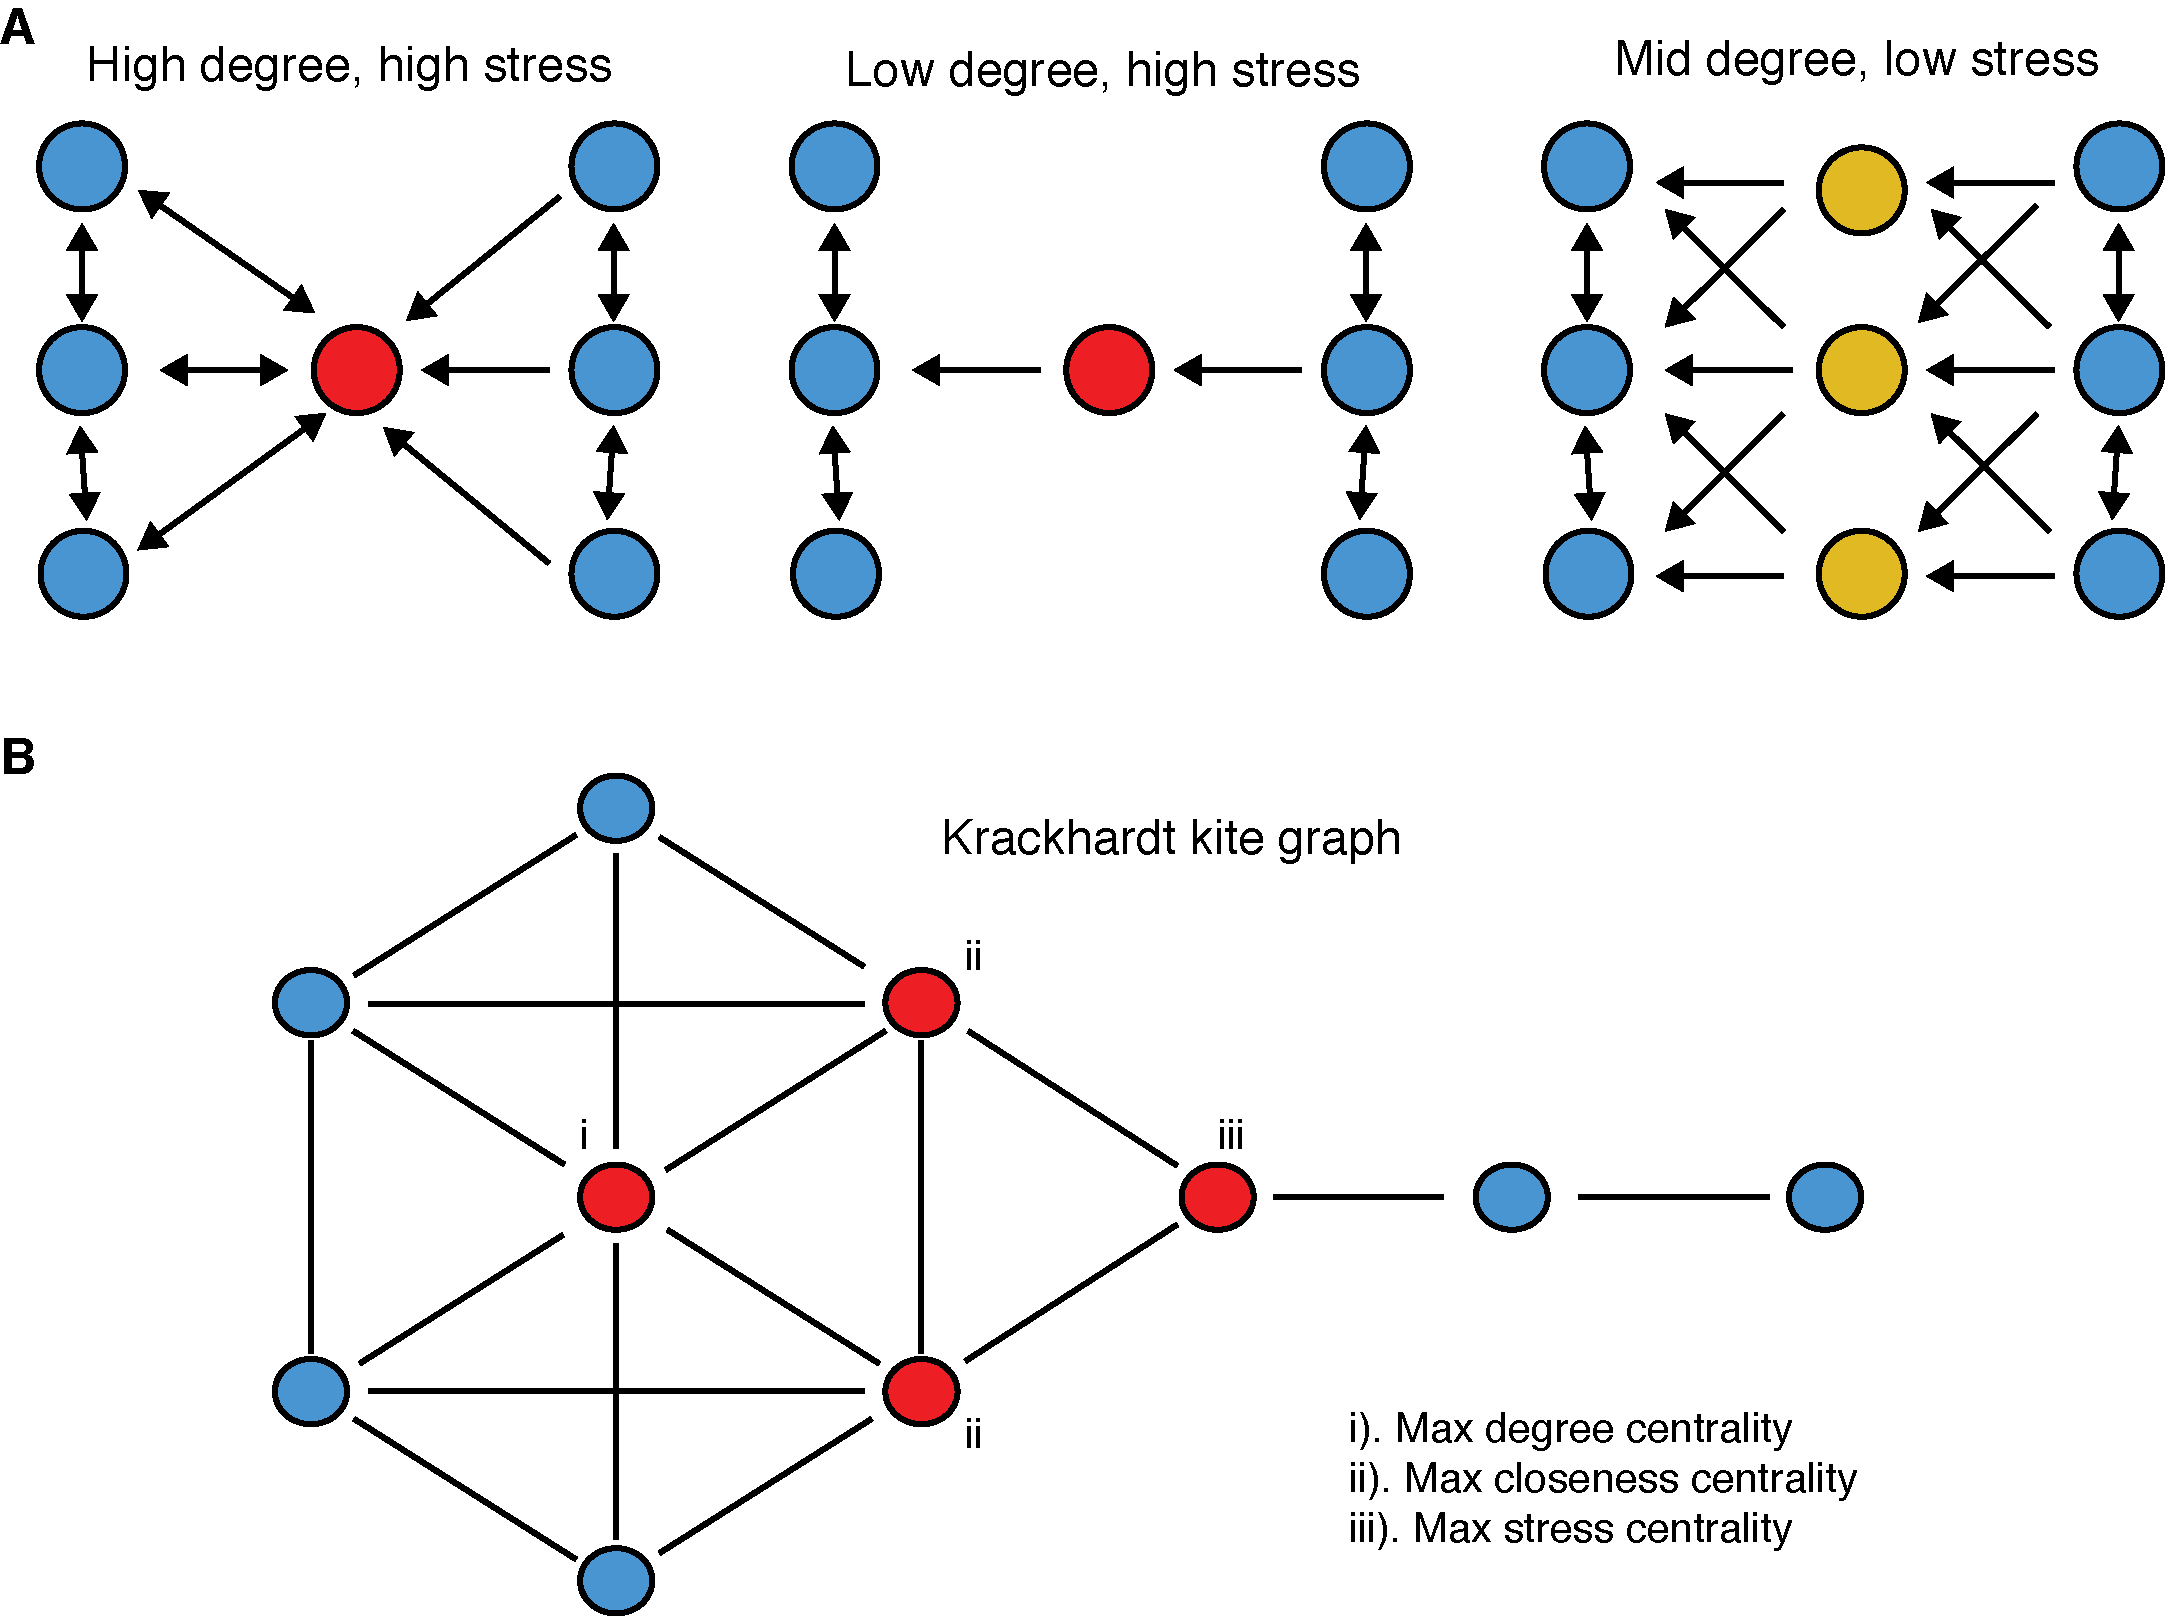
\includegraphics[width=\textwidth,height=\textheight,keepaspectratio]{figures/chapter1/ch1_centrality.png}
    \caption[{Illustration of network centrality measures.}]
    {\textbf{Illustration of network centrality measures.} 
    \textbf{(A)} Schematic of small example networks, exemplifying different levels of degree and stress centrality. Blue nodes are connected nodes in the networks, red and orange nodes are the measured NOIs. Red nodes display high centrality. Orange nodes display low/mid centrality. 
    \textbf{(B)} Krackhardt kite graph \citep{krackhardt_assessing_1990} illustrating how centrality measures emphasise different network structures.
    }
    \label{fig:ch1_stress-example}
\end{figure}

More advanced measures of centrality rely on the concept of "shortest paths". This is determined as the smallest possible number of nodes on a path between two other nodes. Closeness centrality is a measure that calculates the average number of shortest paths from the node of interest (NOI) to other nodes in the network \citep{bavelas_communication_1950}. This assumes that the most important nodes of a network must be generally close to all other nodes in a network. Measures related to this instead quantify how frequently the NOI is an intermediate of a shortest path between all other node pairs in a network. This measure can be represented as the total number of shortest paths (stress centrality), or the fraction of total shortest paths (betweenness centrality), as described in \cite{freeman_set_1977} (Fig. \ref{fig:ch1_stress-example}A). By this method, high stress or betweenness centrality nodes are assumed to exert greater control of communication between other nodes in the network. Different measures of centrality can emphasise different hubs of a network, as exemplified by the Krackhardt kite graph (Fig. \ref{fig:ch1_stress-example}B, \cite{krackhardt_assessing_1990}). Therefore, the choice of centrality measures can offer different conclusions. See Appendix \ref{fig:app_centrality-comparison} for the relationship between centrality measures.

The relevance of centrality measures in biological networks has been well-studied. For example, studies in \textit{S. cerevisiae}, \textit{C. elegans}, and \textit{D. melanogaster} have shown that high centrality can be associated with essential proteins \citep{hahn_comparative_2005, jeong_lethality_2001, koschutzki_centrality_2008}. \cite{hahn_comparative_2005} also noted that highly central proteins evolved more slowly. Interestingly, it has been suggested that nodes with low degree centrality but high stress centrality are more likely to represent nodes connecting distinct network modules (see Fig. \ref{fig:ch1_stress-example}A middle panel, \cite{joy_high-betweenness_2005, koschutzki_centrality_2008}). As such, combining centrality measures can reveal useful information on the structure of regulatory networks.

It is important to note that the networks these studies are based on are comparatively simple relative to mouse or human transcriptional networks, and so may not reflect essentiality as well in more complex organisms. Typically, while centrality is often a good indicator of network structure, it is not always a good indicator of essentiality. This is particularly true for TF models, as TF regulatory logic is complex with highly context dependent binding and function as well as regulatory redundancy (see section \ref{ch1:tf-structure-function}), that is difficult to capture in the GRN model itself. Nevertheless, investigating the centrality of TF hubs offers interesting insights into the complex structure of TF based networks.

\subsection{\label{ch1:grn-motifs}GRN motifs}

GRN models are a complex collection of data and observations. While centrality methods highlight specific regulatory hubs, they do not necessarily describe network structure. The Alon lab pioneered an approach to analysing GRNs by breaking graphs down into simple, repeating units \citep{shen-orr_network_2002, milo_network_2002, mangan_structure_2003}. This analysis focused on the identification of 3-4 node patterns, termed network motifs (or GRN motifs), that were enriched in biological networks. By describing networks in such a way, prominent GRN motifs can be probed whilst still preserving the small-scale structure of the network. Of particular note, these studies found one of the most prominently enriched GRN motifs in biological networks to be the feed-forward loop (FFL, Fig. \ref{fig:ch1_net-motifs}A, \cite{milo_network_2002, mangan_structure_2003}). Another recurring pattern, not specifically enriched in biological networks but important nonetheless, is the TF cascade (Fig. \ref{fig:ch1_net-motifs}B), in which a chain of TFs propagate signal to downstream targets \citep{lee_transcriptional_2002, rosenfeld_response_2003}. 

\begin{figure}[htbp]
    \centering
    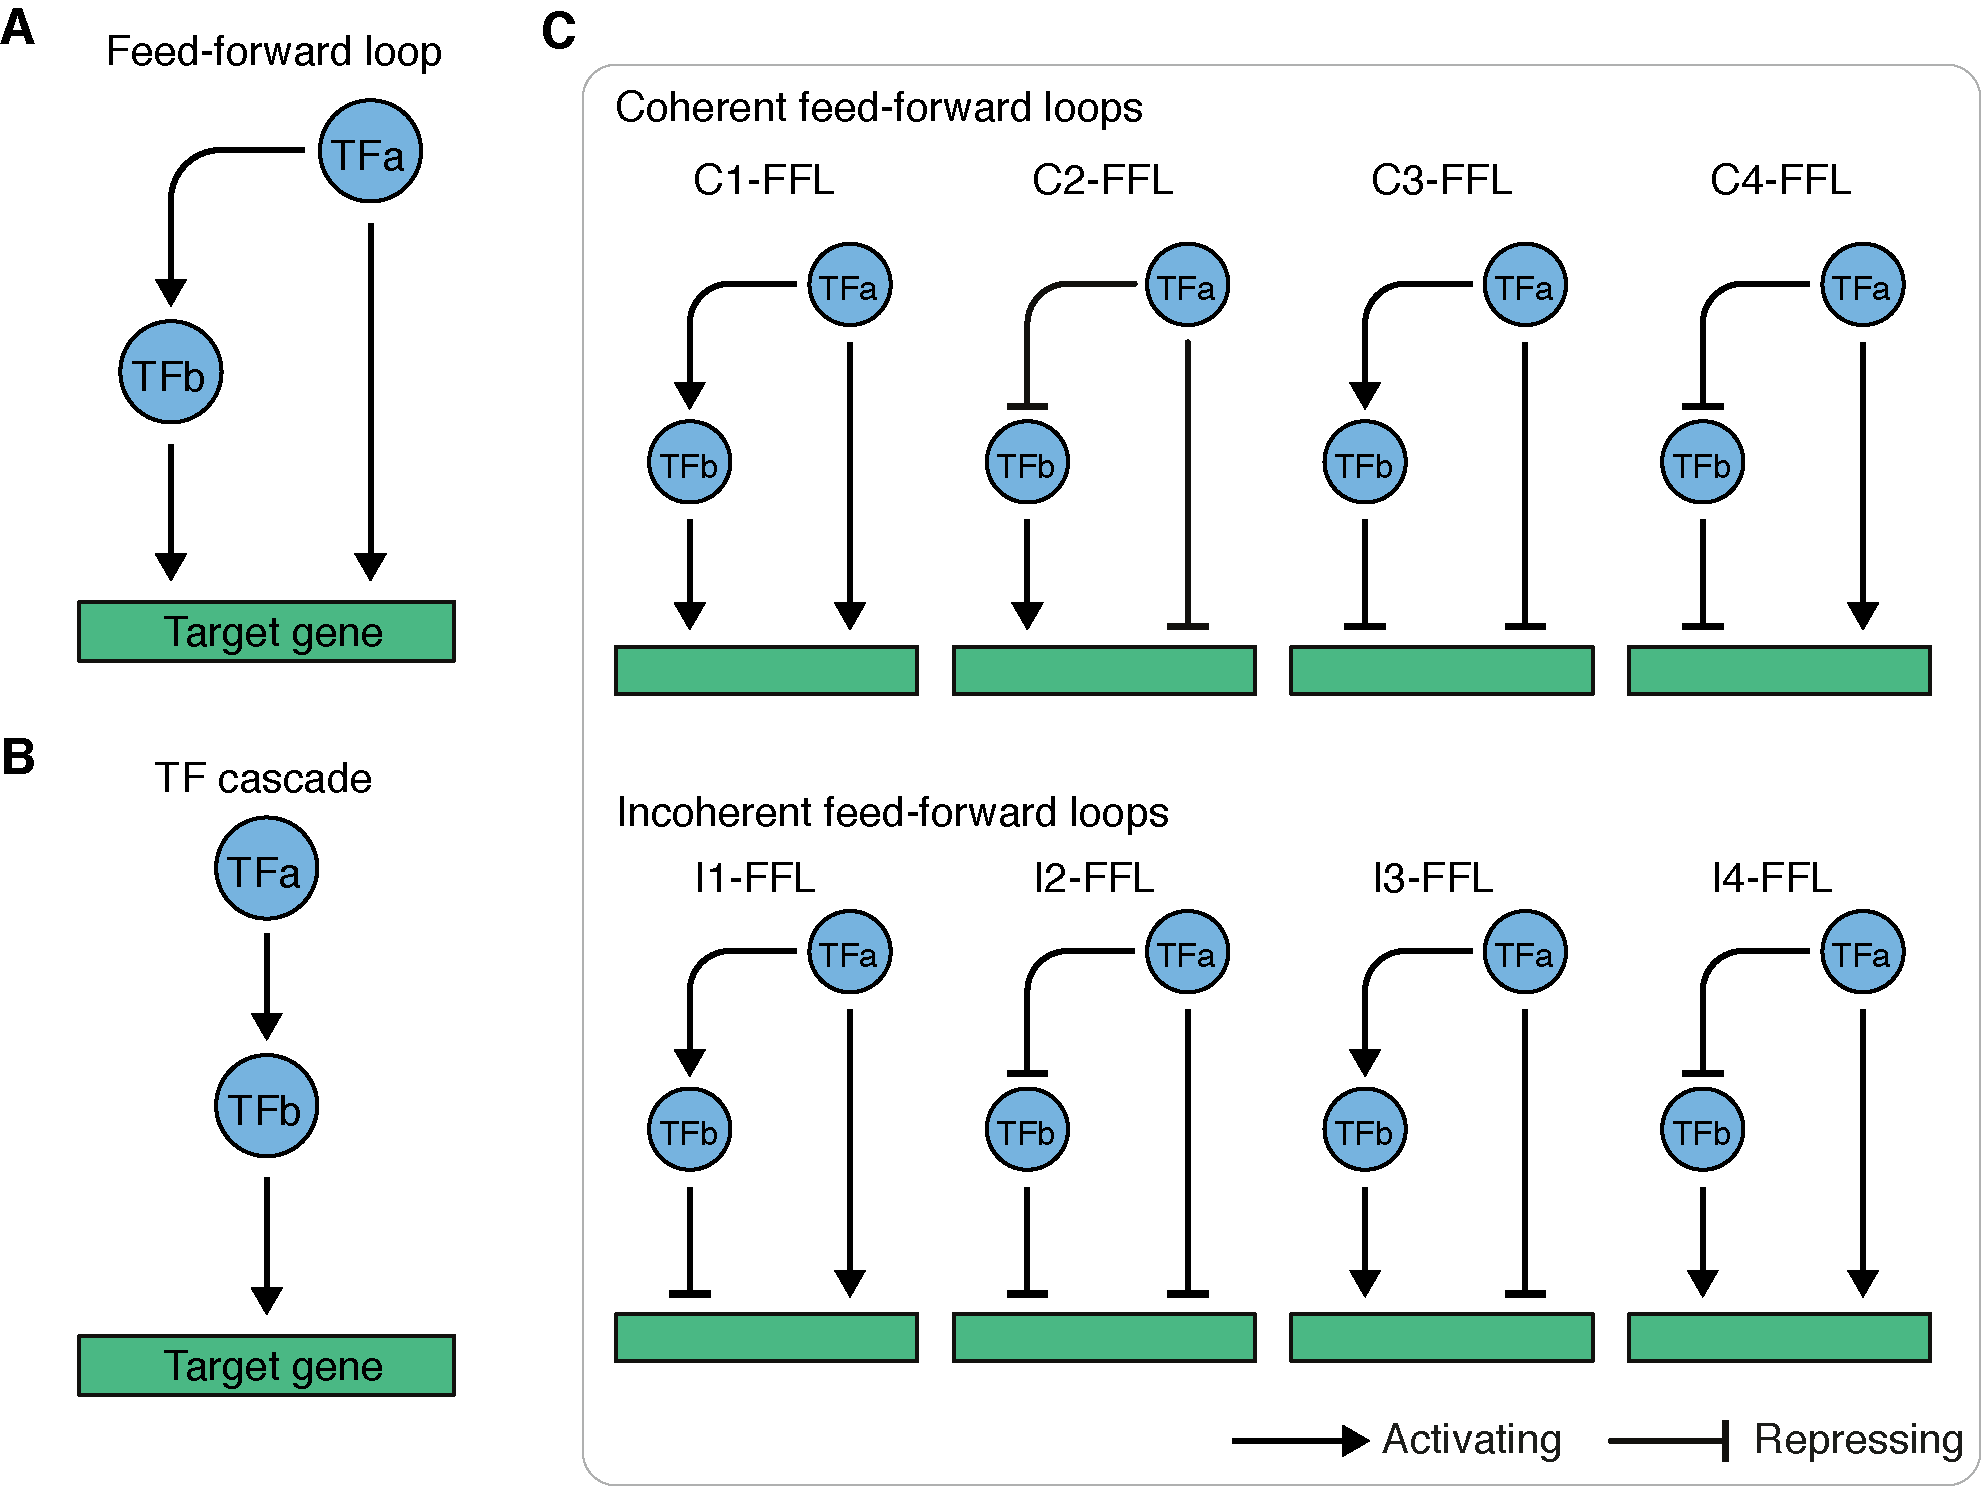
\includegraphics[width=\textwidth,height=\textheight,keepaspectratio]{figures/chapter1/ch1_net-motifs.png}
    \caption[{Illustration of network motifs.}]
    {\textbf{Illustration of network motifs.} 
    \textbf{(A)} Schematic of a FFL circuit.  
    \textbf{(B)} Schematic of a TF cascade. 
    \textbf{(C)} Schematic of coherent (top) and incoherent (bottom) FFL sub-types, determined by sign of effect for each interaction. 
    Blue nodes are TF regulators, green boxes are gene targets
    }
    \label{fig:ch1_net-motifs}
\end{figure}

Many publications have followed these analyses, focusing on the consequence of network structure on interaction dynamics \citep{goentoro_incoherent_2009, joanito_incoherent_2018, mangan_incoherent_2006, mangan_structure_2003}. The FFL can be divided into sub-types based on the sign of effect enacted by the TF regulators (Fig. \ref{fig:ch1_net-motifs}C, \cite{mangan_structure_2003}). This can be broadly grouped into two sub-types, where the regulatory logic of both TF regulators are the same (coherent) or opposite (incoherent). The C1-FFL and I1-FFL motifs (Fig. \ref{fig:ch1_net-motifs}C) were found to be particularly prevalent \citep{joanito_incoherent_2018, mangan_incoherent_2006}. These sub-types can be sub-divided further, as FFLs can be thought to function with AND/OR logic gates. Coherent FFL motifs that exhibit AND logic have been shown to be sign-sensitive delay elements, in that signal processing results in delayed activation going from an OFF to ON state, but rapid deactivation going from ON to OFF \citep{mangan_coherent_2003}. Coherent FFL motifs are also sign-sensitive, with a delay moving from an ON to OFF state \citep{kalir_coherent_2005}. The incoherent I1-FFL has been described as a pulse generator, where the repressive TF (TFb) has a strong effect on gene expression \citep{mangan_structure_2003, basu_spatiotemporal_2004}. This is described as TFa upregulating both TFb and the gene target, followed shortly after by TFb repression of the gene target. 

While GRN motifs are a useful tool for probing networks, and can offer insight into gene regulatory dynamics in small-scale circuits, it is important to acknowledge that these motifs do not always translate to biological function \citep{ingram_network_2006}. Like with measures of centrality, motif structure does not necessarily correlate with importance of a circuit, and to determine regulatory dynamics from GRN motifs detailed biochemical data is needed to support the model, which cannot reasonably be performed genome wide. Despite these drawbacks, GRN motifs are yet another method by which GRN models can be probed, and potentially elucidate key mechanisms of gene regulation.


\subsection{Model systems to apply network analyses}

In this thesis, I have investigated the use of GRN models for investigating the complex behaviour of TF regulation. The application of GRN models to haematopoiesis is an active and evolving field of research \citep{rothenberg_how_2021}. The diverse range of cell types and lineages, and complex transcriptional regulation involved in haematopoiesis makes this an ideal field to probe the use of TF GRNs. In particular, I aim to use GRNs to describe a process underlying the developmental origin of haematopoietic stem cells (HSCs) known as endothelial-to-haematopoietic transition (EHT) \citep{bertrand_haematopoietic_2010, boisset_vivo_2010, kissa_blood_2010} (see section \ref{ch1:eht}). This is a normal haematopoietic process, yet the disruption of normal circuits can sometimes drive disease. Therefore, I also aim to use GRNs to describe \textit{MLL}-rearranged leukaemias (see section \ref{ch1:mllr}), to investigate how normal transcriptional networks may be misregulated in disease. Importantly, EHT is dependent on the TF RUNX1 \citep{okuda_aml1_1996, wang_disruption_1996, north_cbfa2_1999, cai_haploinsufficiency_2000, chen_runx1_2009}, while \textit{MLL}-rearranged leukaemias can involve the overexpression of key TFs, such as \textit{RUNX1} and \textit{MYB}. Therefore, throughout this thesis I aim to anchor GRN analyses on the behaviour of two key TFs: RUNX1 and MYB.

%%%% Normal haematopoietic hierarchy %%%%

%\section{Normal haematopoietic hierarchy}

%Haematopoiesis is a hierarchical process, where all mature haematopoietic populations are derived from haematopoietic stem cells (HSCs).

%%%% Endothelial-to-haematopoietic transition %%%%

\section{\label{ch1:eht}The endothelial-to-haematopoietic transition}

\begin{wrapfigure}{r}{0.5\textwidth}
  \begin{center}
    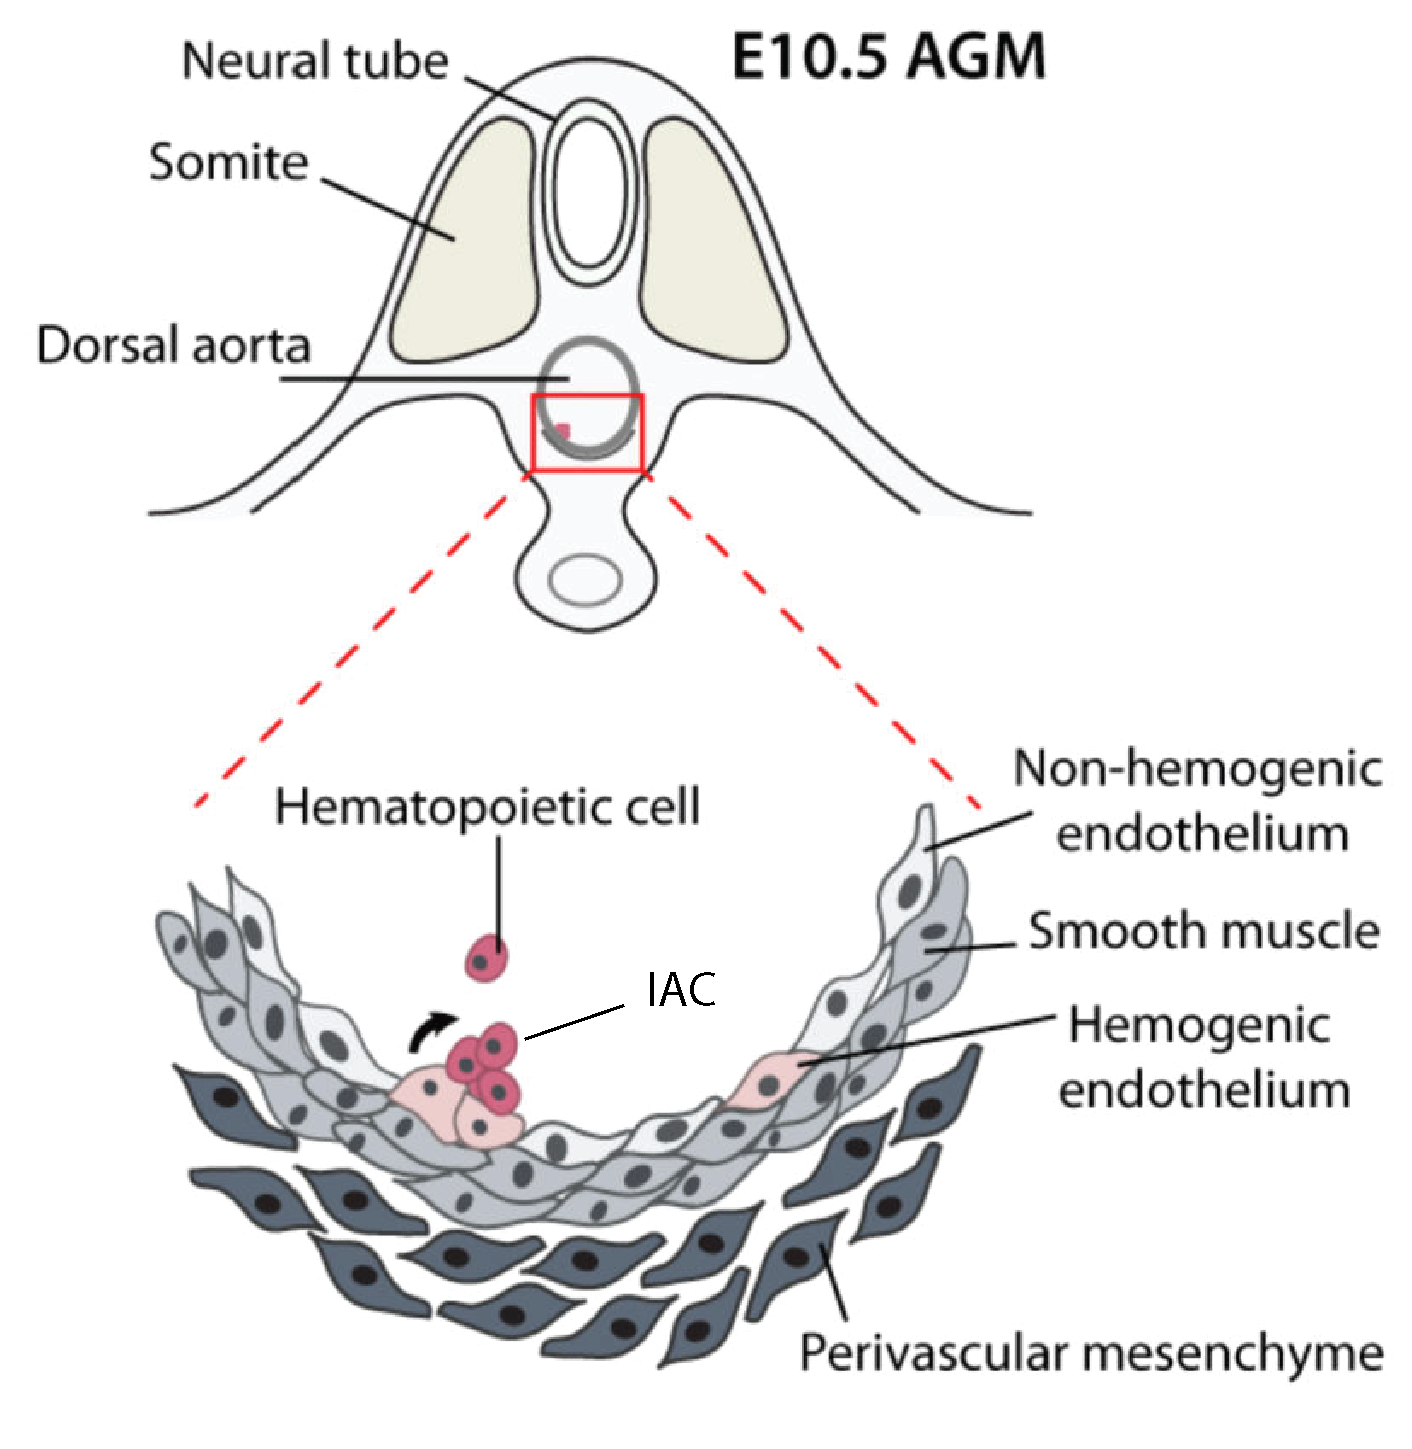
\includegraphics[width=0.48\textwidth]{figures/chapter1/ch1_swiers.png}
  \end{center}
  \caption[{Schematic of EHT at an E10.5 dorsal aorta.}]
    {\textbf{Schematic of EHT at an E10.5 dorsal aorta.} 
    Schematic of an E10.5 AGM, illustrating the EHT process. Boxed section magnified to highlight cell types. HE is coloured as pink, and haematopoietic cells and IACs as red. Non-HE endothelium is coloured as light grey, smooth muscles as mid grey, and mesenchymal cells as dark grey.
    \textit{Figure has been taken from \cite{swiers_short_2013}}.
    }
    \label{fig:ch1_swiers}
\end{wrapfigure}

The establishment of the haematopoietic system occurs in utero, and is a complex process that has been extensively explored in mice. In the embryo, haematopoiesis occurs broadly in three waves. The first, primitive, wave involves the generation of primitive erythroid progenitors originating at yolk sac blood islands from embryonic day E7.0 \citep{palis_development_1999, palis_yolk-sac_2001}. The second wave occurs from E8.25, generating erythro-myeloid progenitors, among others, in the yolk sac \citep{palis_development_1999, frame_erythro-myeloid_2013}. The final wave is established in E10.5 embryos, and occurs within the aorta-gonad-mesonephros (AGM) region at the embryonic dorsal aorta, generating the first adult-type HSCs \citep{medvinsky_definitive_1996, muller_development_1994, de_bruijn_definitive_2000}. The second and final waves establish definitive progenitors (originating from the yolk sac as well as the AGM) that persist into adult life \citep{yoshimoto_autonomous_2012, yoshimoto_embryonic_2011, gomez_perdiguero_tissue-resident_2015, gentek_hemogenic_2018}.

The initial establishment of haematopoietic stem and progenitor cells (HSPCs) occurs by a process referred to as endothelial-to-haematopoietic transition (EHT) \citep{bertrand_haematopoietic_2010, boisset_vivo_2010, kissa_blood_2010}. This process is best described in the embryonic dorsal aorta, but also occurs in the vitelline and umbilical (VU) arteries and the yolk sac \citep{north_cbfa2_1999, zovein_fate_2008, samokhvalov_cell_2007, padron-barthe_clonal_2014, mcgrath_distinct_2015}. It starts with the specification of a specialised subset of endothelial cells (EC) known as haemogenic endothelium (HE). Flat HE cells undergo transcriptional and morphological changes, and bud into the lumen of the dorsal aorta to form intra-aortic clusters (IACs) of cells (Fig. \ref{fig:ch1_swiers}) \citep{boisset_vivo_2010, bertrand_haematopoietic_2010, kissa_blood_2010, swiers_early_2013}. 

Runx1 is a master TF required for definitive haematopoiesis, and more specifically is critical for EHT to occur \citep{okuda_aml1_1996, wang_disruption_1996, north_cbfa2_1999, cai_haploinsufficiency_2000, chen_runx1_2009}. \textit{Runx1} expression begins in HE cells \citep{north_cbfa2_1999}, marking the start of, and commitment to, the haematopoietic program. Importantly, there is an enhancer 23 kb downstream (+23) of \textit{Runx1}, which was found to be a strong driver of reporter gene expression, and to mark both HE and IACs \citep{nottingham_runx1-mediated_2007, bee_nonredundant_2010, ng_runx1_2010}. This +23 enhancer is active in HE as early as E8.5, yet precedes endogenous \textit{Runx1} transcription at this stage \citep{swiers_early_2013}, suggesting the existence of a pre-HE population prior to commitment to the haematopoietic program. 

EHT has been well characterised as a number of specific intermediate cell states following \textit{Runx1} expression in HE, based on various markers and transcriptional profiles. HE and IAC cells undergo maturation through a series of well-defined cell states, classified by CD41, CD43, and CD45 cell surface markers \citep{taoudi_extensive_2008, rybtsov_hierarchical_2011, rybtsov_tracing_2014, ottersbach_endothelial--haematopoietic_2019}. HE first undergoes budding into the lumen of the dorsal aorta and differentiates into a pro-HSC state in E9.5 embryos, with a CD41\upos{}CD43\uneg{} phenotype \citep{rybtsov_tracing_2014}. From E10.5 to E11.5 these pro-HSCs then mature into pre-HSC type I cells with the expression of CD43, and subsequently pre-HSC type II cells with the expression of CD45 \citep{rybtsov_hierarchical_2011, taoudi_extensive_2008}. EHT can also be modelled in vitro, as mouse embryonic stem cells (mESCs) can be induced to differentiate into haematopoietic lineages \citep{galic_t_2006, carpenter_human_2011, woll_human_2009, lu_platelets_2011}, though it is important to highlight it closer represents yolk sac EHT, than dorsal aorta EHT \citep{mcgrath_distinct_2015}.

\subsection{Transcriptional regulation of EHT}

As cells mature through the various EHT states, dynamic transcriptional changes occur \citep{goode_dynamic_2016, ottersbach_endothelial--haematopoietic_2019, swiers_early_2013, solaimani_kartalaei_whole-transcriptome_2015, baron_single-cell_2018, zhu_developmental_2020, zeng_tracing_2019, bergiers_single-cell_2018, gao_transcriptional_2020, vink_iterative_2020, hou_embryonic_2020}. One example involves the Notch signalling pathway, where studies have shown that activation of Notch TFs leads to upregulated \textit{Gata2} and \textit{Runx1}, and subsequent HSC expansion \citep{burns_hematopoietic_2005, robert-moreno_rbpjkappa-dependent_2005, guiu_hes_2013}. While Notch activity is required for activation of essential TFs, it must also be restricted for the progression of pre-HSC I to pre-HSC II cells \citep{souilhol_developing_2016}, highlighting a requirement for tight temporal control of gene expression. Similarly, the TF Sox17 has been found to specify HE identity, yet is considered a repressor of Runx1 and Gata2 function and must be downregulated for EHT progression \citep{clarke_expression_2013, lizama_repression_2015, ottersbach_endothelial--haematopoietic_2019}. 

The regulation of \textit{Runx1} in EHT has been characterised by several studies. Multiple TFs, such as Meis1, Gata2, Tal1, and Ets factors, have been identified to regulate the +23 enhancer \citep{nottingham_runx1-mediated_2007, schutte_experimentally_2016}. Alongside Runx1, \textit{Gata2} expression is also important for the generation of HSCs through EHT, and has a further role in HSC maintenance \citep{tsai_early_1994, ling_gata-2_2004}. Runx1 has also been found to positively autoregulate itself, through interacting with the \textit{Runx1} P1 promoter \citep{martinez_transcriptional_2016}. Specifically within HE, \textit{Runx1} expression has been associated with the activity of genes involved in both cell adhesion and cell migration \citep{lie-a-ling_runx1_2014}, highlighting the potential for Runx1 to drive the morphological changes underpinning the HE budding process. Further, Runx1 is known to upregulate expression of the \textit{Gfi1} and \textit{Gfi1b} TFs, which subsequently leads to a Gfi1/Gfi1b mediated loss of endothelial identity \citep{wilson_gfi1_2010, lancrin_gfi1_2012}. This activity is essential for HE to undergo morphological changes, and is a requirement for haematopoietic development. Runx1 is also well characterised to activate \textit{Spi1} (which encodes PU.1) \citep{huang_pu1_2008}, an essential regulator of later haematopoietic populations that drives myeloid lineage commitment \citep{imperato_runx1pu1_2015}.
 
EHT involves diverse transcriptional changes across several cell type intermediates, and as Runx1 is such an important TF for this to occur, this makes for an exciting system in which to test a GRN model and investigate the role of the Runx1 TF.


\section{\label{ch1:mllr}\textit{MLL}-rearranged leukaemia}

\begin{figure}[!t]
    \centering
    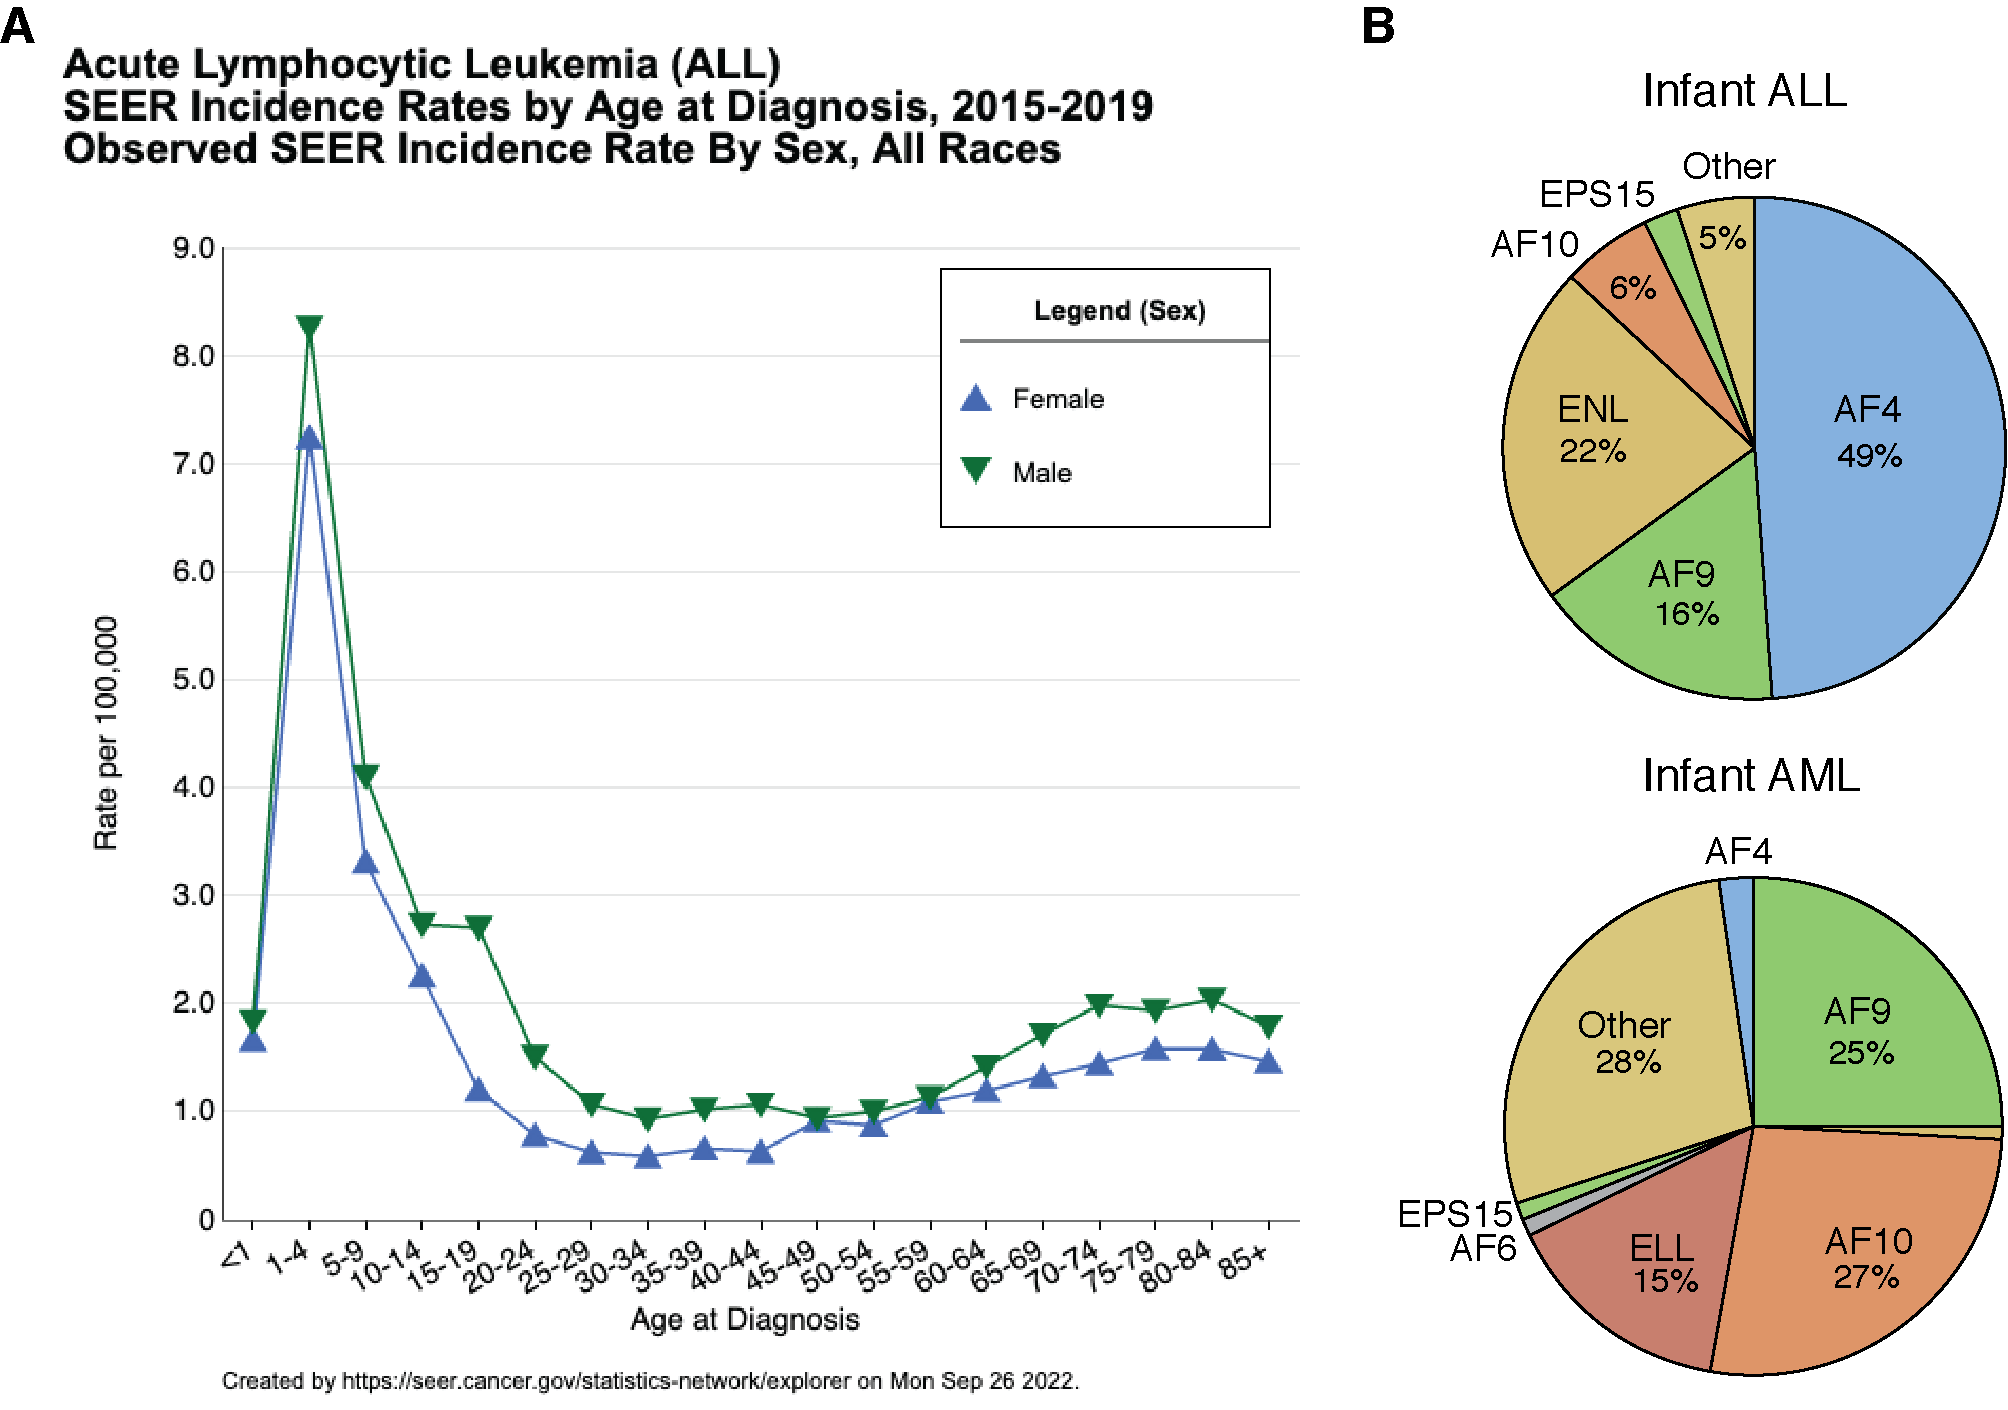
\includegraphics[width=\textwidth,keepaspectratio]{figures/chapter1/ch1_all-incidence.png}
    \caption[{Incidence of ALL and infant \textit{MLL}r fusion partners.}]
    {\textbf{Incidence of ALL and infant \textit{MLL}r fusion partners.} 
    \textbf{(A)} ALL incidence rates by age, based on data collected between 2015 and 2019. \textit{Data and image sourced from the National Cancer Institute (NIH) Surveillance Epidemiology and End Results (SEER) programme \citep{national_cancer_institute_seerexplorer_2022}}. 
    \textbf{(B)} Frequency of \textit{MLL} fusion partners in \textit{MLL}r infant ALL and AML. \textit{Figure adapted from \cite{meyer_mll_2018}}. 
    }
    \label{fig:ch1_all-incidence}
\end{figure}

Leukaemia is a cancer of the blood, of which there are multiple subtypes. Two prevalent subtypes of leukaemia are acute myeloid leukaemia (AML) and acute lymphoblastic leukaemia (ALL). These diseases can affect both young and old people alike, with ALL maintaining a particularly high prevalence in children (Fig. \ref{fig:ch1_all-incidence}A, \cite{national_cancer_institute_seerexplorer_2022, meyer_mll_2018}). Large strides have been made in curing both childhood ALL and AML, however infant leukaemias (patients < 1 year of age) are still associated with a dismal prognosis \citep{rice_mll-rearranged_2020, pieters_outcome_2019}. A particular characteristic of infant leukaemias is the frequency of chromosomal rearrangements at the \textit{Mixed-Lineage Leukemia} (\textit{MLL}, also known as \textit{KMT2A}) gene. These chromosome translocations fuse \textit{MLL} in frame to one of a wide number of partner genes, creating novel fusion proteins (MLL-FPs). While only 10\% of acute leukaemias across all ages carry \textit{MLL} rearrangements (\textit{MLL}r), this frequency rises to 70\% in infant leukaemias \citep{meyer_mll_2013, mann_improved_2010, winters_mll-rearranged_2017, muntean_pathogenesis_2012}. \textit{MLL}r is associated with a poor prognosis, with a 20-40\% 5 year event-free survival, compared to > 60\% in wild-type \textit{MLL} (wt-\textit{MLL}) \citep{winters_mll-rearranged_2017, hilden_analysis_2006, tomizawa_outcome_2007}. Additionally, \textit{MLL}r leukaemias respond poorly to treatment, and 50-60\% of \textit{MLL}r leukaemias in remission result in relapse \citep{winters_mll-rearranged_2017, reaman_treatment_1999, milne_mouse_2017}. There is a clear clinical need to investigate \textit{MLL}r leukaemias, due to the prevalence and severity in infant patients, as well as its resistance to treatment strategies.

Rearrangements of the \textit{MLL} gene can result in translocations with a wide range of partner genes, resulting in unique fusion proteins. In \textit{MLL}r infant ALL (iALL), the most common fusion is between \textit{MLL} and \textit{AF4}, resulting in an MLL-AF4 fusion protein (Fig. \ref{fig:ch1_all-incidence}B, Fig. \ref{fig:ch1_mll-rearrange}A, \cite{meyer_mll_2018}). Conversely, in \textit{MLL}r infant AML, \textit{AF4} is a relatively rare, with \textit{ELL}, \textit{AF10}, and \textit{AF9} accounting for 67\% of \textit{MLL} fusion partners. There are also cases where MLL-AF4 iALLs relapse after treatment, arising as an AML derived from the original leukaemic clone \citep{dorantes-acosta_lineage_2012, gardner_acquisition_2016}. This suggests that while different fusion partners are biased to specific lineages, a single fusion protein can drive both ALL and AML phenotypes.

\subsection{\label{ch1:mll-af4-function}Structure and function of the MLL fusion protein complex}

MLL is an important developmental protein, particularly for haematopoiesis \citep{mcmahon_mll_2007, crump_why_2019}. MLL is a methyltransferase that methylates histone H3 lysine 4, and this activity is driven through its SET domain, which was found to be important for wt-MLL upregulation of \textit{Hox} genes \citep{milne_mll_2002, nakamura_all-1_2002}. \textit{MLL} translocations involve the fusion of N-terminus MLL to the C-terminus of a partner protein, resulting in loss of the SET domain and wt-MLL methyltransferase activity (Fig. \ref{fig:ch1_mll-rearrange}B, \cite{winters_mll-rearranged_2017, zeleznik-le_11q23_1994}). However, the DNA binding activity of wt-MLL is mostly harboured within the N-terminus, and as such MLL binding affinities strongly direct binding of the MLL-FP \citep{winters_mll-rearranged_2017, zeleznik-le_11q23_1994}. This consists of a CxxC domain, which binds unmethylated CpG (uCpG) islands \citep{birke_mt_2002}, as well as multiple AT-hooks that promote binding to AT-rich DNA \citep{zeleznik-le_11q23_1994} (Fig. \ref{fig:ch1_mll-rearrange}B). DNA binding is also thought to be driven through N-terminal MLL recruitment of Menin, and subsequently LEDGF, as LEDGF binds H3K36me2 marks \citep{hughes_menin_2004, milne_menin_2005, yokoyama_menin_2008, zhu_ash1l_2016}, though this has been shown to be dispensable for targeting to the \textit{HOXA9} gene \citep{milne_multiple_2010}. The C-terminus of wt-MLL also contains multiple plant homeodomain (PHD) fingers and a bromodomain that contribute to chromatin binding (Fig. \ref{fig:ch1_mll-rearrange}B), and are lost in the MLL-FP \citep{zeleznik-le_11q23_1994}.

\begin{figure}[htbp]
    \centering
    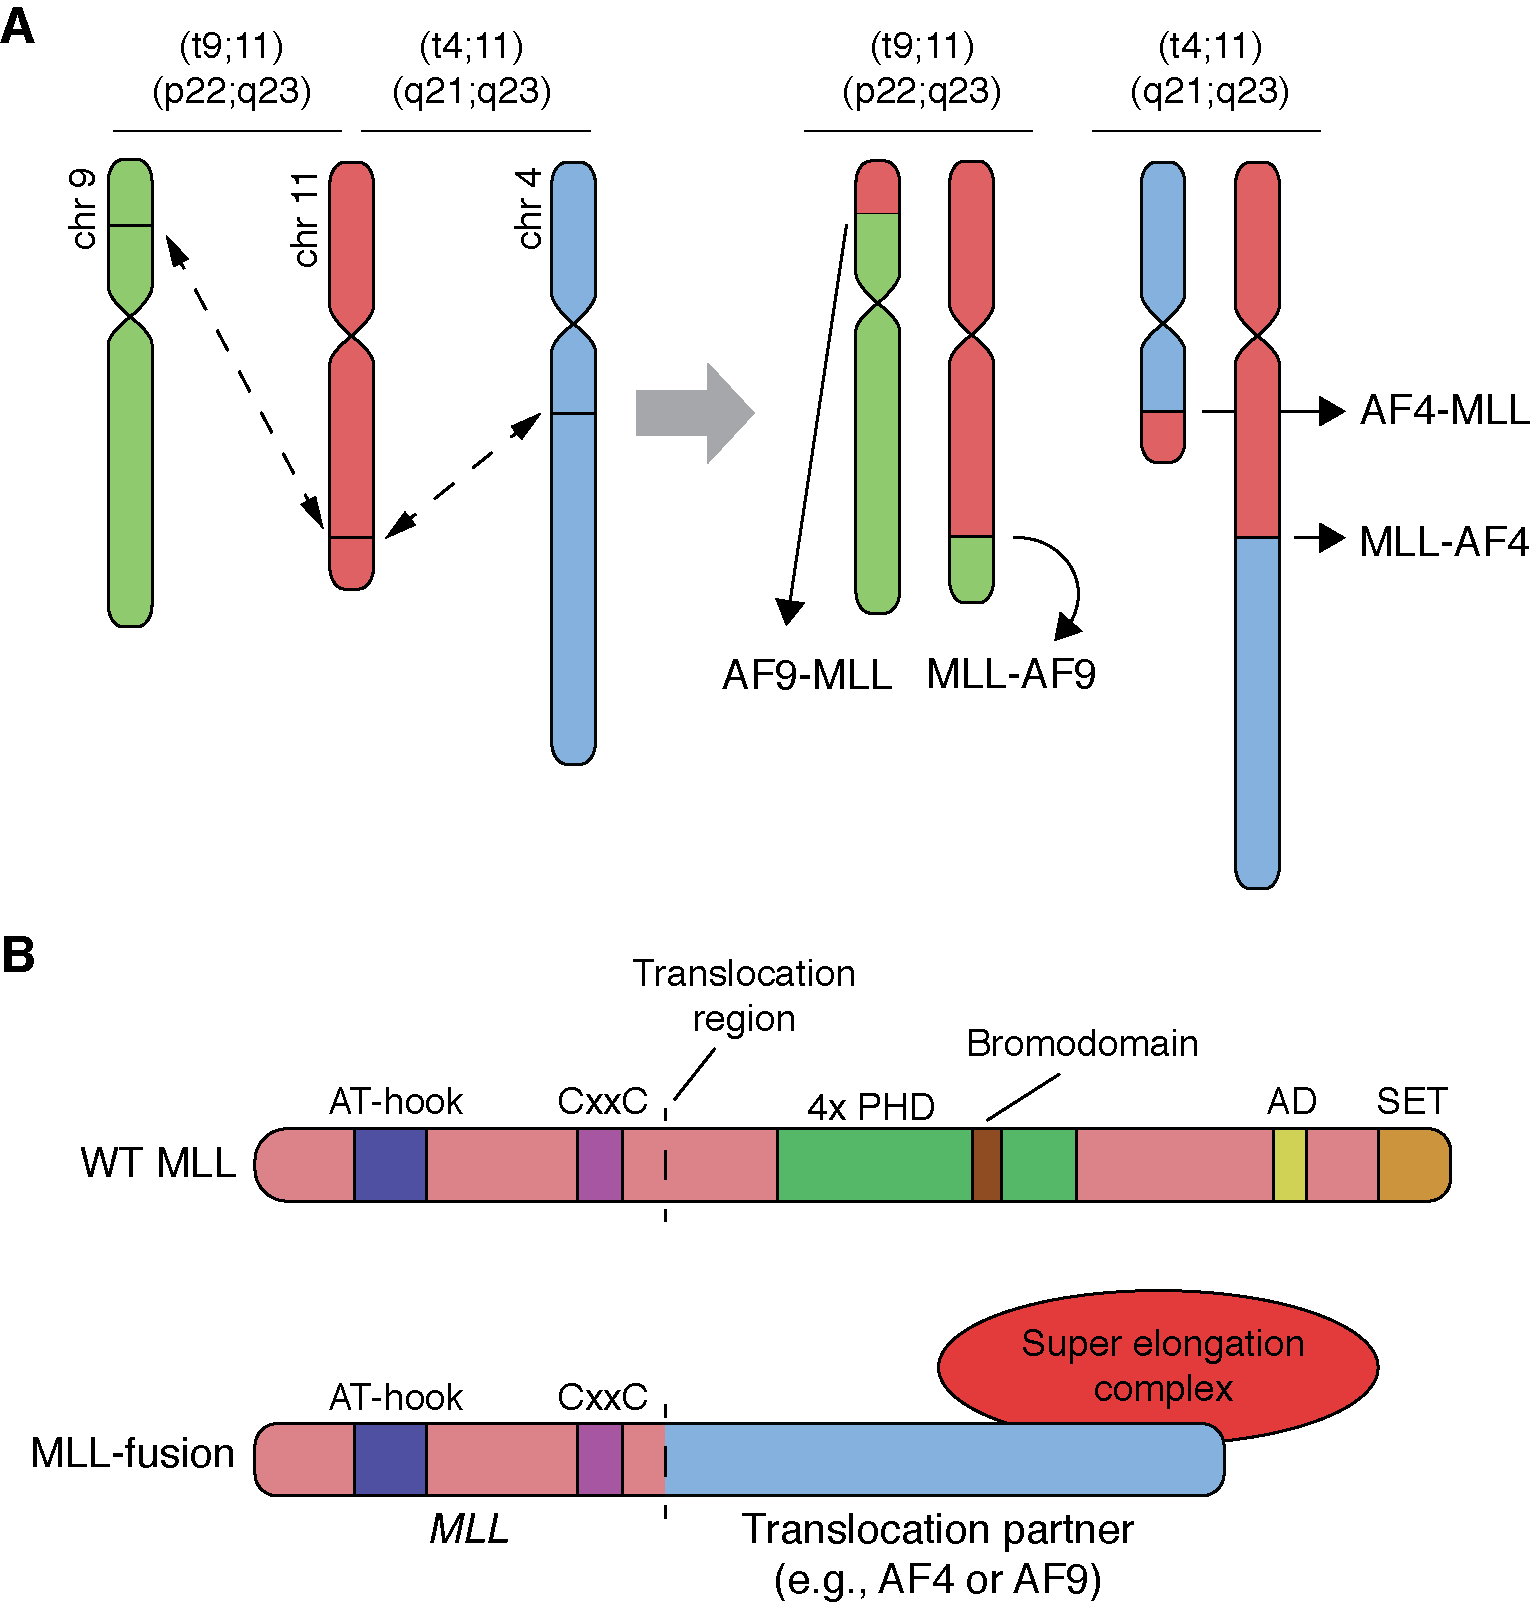
\includegraphics[width=0.8\textwidth,keepaspectratio]{figures/chapter1/ch1_mll-rearrange.png}
    \caption[{Schematic of \textit{MLL} translocations, and wild type and MLL fusion protein structure.}]
    {\textbf{Schematic of \textit{MLL} translocations, and wild type and MLL fusion protein structure.} 
    \textbf{(A)} Schematic of the chromosomal rearrangements resulting in MLL-AF4 and MLL-AF9 fusion proteins. \textit{MLL} is located on chromosome 11, and \textit{AF4} and \textit{AF9} are located on chromosome 4 and 9, respectively. Horizontal black lines on chromosomes indicate the translocation break points. Dashed lines indicate translocation. 
    \textbf{(B)} Simplified schematic of MLL fusion protein structure, adapted from \cite{winters_mll-rearranged_2017}.
    }
    \label{fig:ch1_mll-rearrange}
\end{figure}

Both MLL-AF4 and MLL-AF9 fusion proteins drive transcription through the recruitment of various factors, driven through the AF4 or AF9 C-terminus. Importantly, this includes the recruitment and assembly of a super elongation complex (SEC) that drives gene transcription (Fig. \ref{fig:ch1_mll-rearrange}B), consisting of both AF4 and AF9, as well as AFF4, ENL, ELL1, ELL2, and ELL3, among others \citep{lin_aff4_2010, smith_super_2011, lin_dynamic_2011, ballabio_molecular_2012, takahashi_molecular_2020, slany_mll_2020, yokoyama_higher-order_2010}. This complex contains multiple common MLL fusion partners, and as such highlights how different MLL-FPs can have similar behaviours by recruiting a similar overall complex. The MLL-FP complex also recruits Disruptor of Telomeric Silencing 1-like (DOT1L) \citep{bernt_mll-rearranged_2011, biswas_function_2011, lacoste_disruptor_2002, milne_leukemogenic_2005, okada_hdot1l_2005, mueller_role_2007, slany_mll_2020, lin_instructive_2016, krivtsov_h3k79_2008}, which is a methyltransferase for H3 lysine 79 (H3K79) \citep{steger_dot1lkmt4_2008}. H3K79 methylation has been associated with strong transcriptional overexpression at a subset MLL-FP targets, such as \textit{HOXA9} and \textit{RUNX1}, and perturbation of DOT1L activity significantly downregulates gene expression \citep{kerry_mll-af4_2017, godfrey_dot1l_2019, milne_leukemogenic_2005, wilkinson_runx1_2013}. Additionally, in \textit{MLL}r leukaemia H3K79me is also found enriched at a subset of intragenic enhancers, and maintains enhancer-promoter (E-P) interactions \citep{godfrey_dot1l_2019}. A related cofactor that is associated with the MLL-FP complex, though not directly recruited, is BRD4. BRD4 binds acetylated chromatin via its bromodomain \citep{dey_double_2003}, but in addition to this it was found that BRD4 was associated with members of the SEC, and further that BRD4 was a potential therapeutic target for MLL-AF9 leukaemias \citep{dawson_inhibition_2011, zuber_rnai_2011}. BRD4 directly interacts with P-TEFb and stimulates transcription by increasing P-TEFb dependent Pol II phosphorylation \citep{yang_recruitment_2005, jang_bromodomain_2005}. It has also been reported that DOT1L and BRD4 functionally cooperate in MLL leukaemias, through EP300 acetylating H4K5 at methylated H3K79 regions, and subsequent BRD4 recruitment to the acetylated chromatin \citep{gilan_functional_2016}. 

An interesting feature of MLL-FPs, most characterised with MLL-AF4, is the observation that at a subset of gene targets MLL-AF4 binds to uCpG promoters then spreads into the gene body \citep{kerry_mll-af4_2017}. These "spreading targets" are highly overexpressed, and spreading is associated with enriched Menin and H3K79 methylation. Interestingly, these overexpressed targets were also highly susceptible to DOT1L inhibition, highlighting DOT1L as key driver at this subset of targets.

\subsection{Transcriptional impact of MLL fusion proteins}

As MLL-AF4 and MLL-AF9 recruit a SEC, and are associated with transcriptional coactivators (i.e., BRD4), these fusion proteins are considered to act as drivers of gene transcription rather than repressors. Interestingly, \textit{MLL}r leukaemias are associated with few or no cooperating mutations \citep{andersson_landscape_2015, the_cancer_genome_atlas_research_network_genomic_2013, bardini_dna_2010, bardini_implementation_2011}, suggesting that the MLL fusion protein alone is sufficient to drive leukaemogenesis. In fact, numerous studies have shown that expression of MLL-AF4 or MLL-AF9 is sufficient to induce leukaemia \citep{rice_human_2021, krivtsov_h3k79_2008, krivtsov_cell_2013}. As MLL fusion proteins function by overexpressing genes, and are sufficient on their own for leukaemogenesis, \textit{MLL}r leukaemias may be considered to be an entirely transcriptionally driven disease. This makes for an ideal system to probe aberrant gene expression profiles with a GRN approach.

\textit{BCL2} is an MLL-AF4 and MLL-AF9 target of particular importance. It has been reported that not only does MLL-AF4 bind to the \textit{BCL2} promoter, but also a downstream enhancer, resulting in overexpression of the gene \citep{godfrey_mll-af4_2017, benito_mll-rearranged_2015}. MLL-AF4 leukaemias are highly sensitive to \textit{BCL2} perturbation \citep{robinson_abundant_2008}, in keeping with the role of BCL-2 in deterring apoptosis \citep{czabotar_control_2014, singh_regulation_2019}. This highlighted \textit{BCL2} as a key gene in cell survival. As such, venetoclax, a drug targeting BCL-2 protein, has been a successful treatment of MLL-AF4 leukaemias \citep{benito_mll-rearranged_2015, khaw_venetoclax_2016, niu_acute_2014}. 

MLL-AF4 and MLL-AF9 have also been found to overexpress \textit{MYC}, a TF and oncogene that drives proliferation \citep{dang_myc_2012, prange_mll-af9_2017}. \textit{MYC} overexpression typically results in apoptosis, either through indirectly activating p53 (p53-dependent) or modulating the balance between pro-apoptosis and anti-apoptotic factors (p53-independent) \citep{fairlie_co-operativity_2021}. However, the overexpression of \textit{BCL2} prevents activation of the p53-independent apoptotic pathway, allowing MLL-AF4 and MLL-AF9 to upregulate \textit{MYC} and increase proliferation. \citep{fairlie_co-operativity_2021, fanidi_cooperative_1992, bissonnette_apoptotic_1992}. As such, both \textit{BCL2} and \textit{MYC} must be expressed for the full leukaemic potential of \textit{MLL}r leukaemias.

Another key gene is \textit{PROM1} (encoding CD133 protein), which is an MLL-AF4 spreading target that is important for leukaemic growth \citep{kerry_mll-af4_2017, mak_mixed_2012, godfrey_h3k79me23_2021}. Interestingly, it was found that not only does MLL-AF4 drive expression through the promoter, but H3K79 methylation deposited by DOT1L at an intragenic enhancer was found to maintain E-P interactions, potentially enhancing promoter activity \citep{godfrey_h3k79me23_2021}. Further, this intragenic enhancer also interacted with a nearby gene \textit{TAPT1}, highlighting the capacity for complex regulation driven by MLL-AF4, not just through promoter binding, but modulation of enhancer activity and E-P interactions.

RUNX1 and MYB are two TFs of particular interest. \textit{RUNX1} is overexpressed in MLL-AF4 ALL leukaemia, and is an MLL-AF4 spreading target \citep{wilkinson_runx1_2013, kerry_mll-af4_2017}. It has also been found that \textit{RUNX1} perturbation is detrimental for leukaemic growth \citep{wilkinson_runx1_2013}. While RUNX1 itself is a potent transcriptional regulator, \cite{wilkinson_runx1_2013} suggested an additional regulatory mechanism whereby RUNX1 interacts with the AF4-MLL (the reciprocal fusion protein of MLL-AF4) complex. MYB is a known to be upregulated by MLL-AF9 in MLL-AF9 AML, after which these AML become addicted to MYB \citep{zuber_integrated_2011}. Both RUNX1 and MYB are expressed in numerous haematopoietic populations, in addition to the critical role of RUNX1 in EHT (section \ref{ch1:eht}), and are important regulators of several lineages \citep{ichikawa_role_2013, wang_myb_2018}. Probing the activity of these deregulated TFs in leukaemia will be important to fully understand the regulation of these diseases, as well as how aberrantly expressed transcriptional networks contribute to leukaemogenesis.

\section{Thesis overview and aims}

In this thesis I have focused on the application of GRN models to investigate gene regulation in a normal developmental process, and gene regulation in aberrantly regulated processes, most notably leukaemia. Gene regulation is complex to model in vivo, and TFs add a layer of complexity that is difficult to address. The specific combination of TFs, not just expressed in a cell but bound at a specific genomic locus, can drastically alter regulatory output. This specific combinatorial code underpins all developmental processes, can drive change in cell identity, and can be a critical component for understanding how diseases are driven.

Haematopoiesis involves complex gene regulation and multiple lineages, and cell identity is relatively plastic, with cells capable of being reprogrammed into different lineages \citep{schutte_experimentally_2016, riddell_reprogramming_2014, batta_direct_2014}. As a result, it is also an active field of research for applying GRN models \citep{rothenberg_how_2021}. EHT is a particularly interesting process associated with the developmental origin of HSCs, that requires dose-specific and temporally controlled activation of TFs and dynamic regulation of gene expression. However, the disruption of normal regulatory processes can result in disease, as seen with \textit{MLL}r acute leukaemias. MLL-AF4 and MLL-AF9 leukaemias are interesting haematopoietic malignancies, that are unique in being driven by a single translocation event and are a transcriptional disease \citep{andersson_landscape_2015, the_cancer_genome_atlas_research_network_genomic_2013, bardini_dna_2010, bardini_implementation_2011, rice_human_2021, krivtsov_h3k79_2008, krivtsov_cell_2013}. 

The well-defined populations of EHT and dynamic gene regulation make for a promising system to probe using GRN approaches. As the RUNX1 TF is critically required for EHT, it is a pivotal TF to investigate in this GRN. \textit{RUNX1} is also an important MLL-AF4 target overexpressed in \textit{MLL}r ALL, and as such \textit{MLL}r leukaemias represent a system in which RUNX1 behaviour can be studied within a misregulated, leukaemic GRN. Studying GRN models of these systems offers an interesting view of RUNX1 behaviour in different contexts: normal and aberrant haematopoiesis. MYB is also an interesting TF that, while not critical for EHT, is an essential overexpressed gene MLL-AF9 AML. Studying GRN models with a view of RUNX1 and MYB behaviour, with a particular focus on how these TFs cooperate with other regulators, will offer interesting comparisons.
%\clearpage

\noindent
There are three questions central to this thesis project: 

\vspace*{-5mm}
\begin{enumerate}
    \item What novel regulatory mechanisms underpinning key processes can be understood using GRN models?
    \item What insight into TF combinatorial logic and regulatory synergy driving processes do these GRNs offer?
    \item How are normal transcriptional networks deregulated in \textit{MLL}r leukaemia?
\end{enumerate}

\vspace*{-5mm}
I have established and explored a model of EHT regulation in chapter \ref{chapter3_EHT} to investigate key regulatory interactions involving Runx1, and to probe cases of TF cooperation that may underlie the EHT process. Further, in this chapter I have explored the EHT in relation to the pre-HE population, and identified genes characterising this population, and TFs that may drive activity of the +23 \textit{Runx1} enhancer at this early stage. I have also generated a model of MLL-AF4 and RUNX1 leukaemia in chapter  \ref{chapter4_MA4}, where I have explored key drivers of MLL-AF4 ALL, and the specific cooperation between MLL-AF4 and RUNX1, as well as RUNX1 and MYB. This work was extended in chapter \ref{chapter5_normToLeuk}, where I have investigated the leukaemic transformation of a normal granulocyte-monocyte progenitor (GMP) GRN after inducing \textit{MLL-AF9} expression. This final chapter attempts to explore how a normal GRN can be transformed over time, following induction of leukaemia. 

This study serves to further our knowledge of the regulation of EHT, particularly through combinatorial logic. It also improves our understanding of the pre-HE population, and offers insight into the potential early regulators of the +23 \textit{Runx1} enhancer. Through studying MLL-AF4 and MLL-AF9 leukaemias, this thesis highlights concepts characterising the perturbation of normal GRNs in \textit{MLL}r leukaemia, driven in part through TF cooperation.
















% Irrelevant but maybe for padding:

%\subsection{The role of RUNX1 in lymphoid and myeloid malignancies}
%•	Overview of lymphoid and myeloid leukaemia’s
%•	RUNX1 mutations and fusions
%•	RUNX1 is overexpressed in MLL-rearranged leukaemia’s







\chapter{\label{chapter2_methods}Materials and methods} 
\chaptermark{Chapter 2 - Materials and methods}

\begingroup
\raggedright
\minitoc
\endgroup

\section{Mouse husbandry}

All procedures involving mice were in compliance with UK Home Office regulations and the Oxford University Clinical Medicine Ethical Review Committee. Mice were housed in individually ventilated cages with free access to food and water and maintained in a 12-hour light-dark cycle.

\section{Embryo studies}

\subsection{\label{ch2:embryo-collection}Timed matings and embryo collection}

Timed pregnancies were generated through overnight mating. To acquire transgenic embryos, matings were set up with (CBA × C57BL/6)/F1 females and 23GFP (\textit{Runx1} +23 GFP enhancer reporter) transgenic males (maintained on a mixed (CBA × C57BL/6) background). To acquire wild type embryos, matings were set up with (CBA × C57BL/6)/F1 females and (CBA × C57BL/6)/F1 males. Confirmation of a vaginal plug after overnight mating was marked embryonic day (E)0.5. At the appropriate developmental time point, mice were killed by a Schedule 1 method and embryos extracted from the uteri, and staged by somite pairs. 

\subsection{\label{ch2:embryo-dissection}Embryo tissue dissection and cell sorting}
Embryo dissections for RNA-seq and ATAC-seq experiments (chapter \ref{chapter3_EHT}) were performed as previously described \citep{swiers_early_2013} by members of the de Bruijn lab. Para-aortic splanchnopleura (PAS)/AGM and VU vessels were dissected from E8.5 (PAS only), E9.5 and E10.5 embryos in PBS supplemented with 10\% fetal calf serum (FCS), 50 U/ml penicillin, and 50 \microg{}/ml streptomycin (Gibco). PAS/AGM+VU tissues were pooled and incubated for 15 min at 37°C in PBS without calcium or magnesium, containing 10\% FCS, 50 U/ml penicillin, 50 \microg{}/ml streptomycin, and 0.1\% (w/v) type I collagenase (Sigma). Cells were disassociated by gentle pipetting. 

Cells were washed, resuspended, and incubated in an antibody cocktail (Table \ref{tbl:ch2_mesc-ab}) optimally diluted in 10\% FCS/PBS. Cells were incubated for 30 min 4°C, washed, and resuspended in 10\% FCS/PBS with 1/1000 Hoechst 33258 (Thermo fisher) to stain dead cells. Haematopoietic populations were isolated by fluorescence-activated cell sorting (FACS) on a BD FACSAria Fusion. Sorted phenotypes include E8.5 endothelial cells (EC, Ter119\uneg{}VECad\upos{}CD41\uneg{}CD45\uneg{}23GFP\uneg{}) and pre-HE (Ter119\uneg{}VECad\upos{}CD41\uneg{}CD45\uneg{}23GFP\upos{}), E9.5 HE (Ter119\uneg{}VECad\upos{}\-CD41\uneg{}CD45\uneg{}23GFP\upos{}) and pro-HSC/haematopoietic progenitors (Ter119\uneg{}VECad\upos{}CD41\upos{}CD45\uneg{}), and E10.5 pre-HSC I (Ter119\uneg{}VECad\upos{}\-CD41\upos{}CD45\uneg{}) and pre-HSC II (Ter119\uneg{}VECad\upos{}CD41\upos{}CD45\upos{}). Instruments were set up using unstained and single stain controls and sort gates were drawn according to fluorescent minus one (FMO) controls. All sorts were done by the staff of the WIMM Flow Cytometry core facility. 

    \begin{table}[ht]
    \centering
    \caption{Antibodies used for flow cytometry analysis and FACS sorting of EHT cell populations.}
    \begin{tabular}{@{}lllll@{}}
    \toprule
    \textbf{Target} & \textbf{Conjugate} & \textbf{Dilution} & \textbf{Catalogue   number} & \textbf{Company} \\ \midrule
    CD41 & PE & 1:400 & 558040 & Pharmigen \\
    CD45 & APCef780 & 1:200 & 13-5821-81 & eBioscience \\
    Ter119 & PE-Cy7 & 1:200 & 557853 & Pharmigen \\
    VE-cadherin & APC & 1:200 & 17-1441-82 & eBioscience \\ \bottomrule
    \end{tabular}
    \caption*{All antibodies reactive in mouse, and raised in rat.}
    \label{tbl:ch2_mesc-ab}
    \end{table}
    
\subsection{Whole mount immunofluorescence imaging}

Embryos at day E8.5 were processed for whole-mount immunofluorescence analysis as described in \cite{yokomizo_whole-mount_2012}. Embryos were fixed in 4\% paraformaldehyde for 30 min 4°C, then washed with PBS 3x 10 min each. Embryos were dehydrated by 1x 50\% methanol/PBS 10 min, followed by 2x 100\% methanol 10 min washes. Dehydrated embryos were stored at -20°C. 

Before antibody staining, embryos were rehydrated by 1x 50\% methanol/PBS 10 min, followed by 2x PBS 10 min washes. Embryos were kept in the dark during all wash and incubation steps. Embryos were incubated with blocking buffer (0.4\% triton X-100, 10\% FCS in PBS) for 3 hours 4°C to block non-specific binding of antibodies. Primary antibodies were diluted in blocking buffer (see table \ref{tbl:ch2_whole-mount-ab}), and embryos were incubated with 200 \microl{} antibody mix overnight at 4°C with rocking. Embryos were washed 3x with blocking buffer for 2 hours each wash. Secondary antibodies were diluted in blocking buffer (see table \ref{tbl:ch2_whole-mount-ab}), and embryos were incubated with 200 \microl{} antibody mix overnight at 4°C with rocking. Embryos were washed 3x with blocking buffer for 2 hours each wash. Embryos were washed 3x 20 min with PBS with 0.4\% triton-X 100. Embryos were dehydrated in methanol, as above. Using molten 1\% agarose, embryos were anchored onto a coverslip with a FastWell reagent barrier (664113-GRA, Grace Bio-Labs) sealed, and the FastWell was filled with methanol. Embryos were washed 3x 1 min with methanol. A 1:1 solution of benzyl alcohol (\#402834, Sigma) and benzyl benzoate (\#0215483990, MP Biomedicals) was prepared (BABB solution). Embryos were washed 3x 1 min with a 50\% methanol and 50\% BABB solution. 100\% BABB solution washes were performed until the embryos were sufficiently clear. A coverslip was applied to the surface of the FastWell, and sealed with nail polish to prevent leakage. 

Image acquisition was performed using a Zeiss AXIO Observer.Z1 inverted microscope equipped with a Zeiss LSM-880 confocal system using an 25x LDLCI PlnApo NA:0.8 DI objective. Image acquisition settings were adjusted on the basis of unstained, single stain, and FMO controls.

    \begin{table}[ht]
    \caption{Antibodies used for whole-mount immunofluorescence.}
    \resizebox{\textwidth}{!}{
    \begin{tabular}{@{}llllll@{}}
    \toprule
    \textbf{Target} & \textbf{Conjugate} & \textbf{Dilution} & \textbf{Raised in} & \textbf{Catalogue number} & \textbf{Company} \\ \midrule
    CD31 & Unconjugated & 1:200 & Goat & AF3628 & R\&D Systems \\
    GFP & Unconjugated & 1:200 & Chicken & ab13970 & Abcam \\
    CD109 & Unconjugated & 1:100 & Rabbit & 24765S & Cell Signaling \\
    anti-Goat IgG & AF647 & 1:200 & Donkey & A21447 & Invitrogen \\
    anti-Chicken IgG & AF488 & 1:200 & Donkey & 703-545-155 & Jackson \\
    anti-Rabbit IgG & AF594 & 1:200 & Donkey & A21207 & Invitrogen \\ \bottomrule
    \end{tabular}
    }
    \label{tbl:ch2_whole-mount-ab}
    \end{table}


\section{Cell culture}

All cell lines were grown in a 37°C humidified incubator with 5\% CO\textsubscript{2}, and were confirmed to be free of mycoplasma.

\subsection{Culturing mESCs}

Mouse embryonic stem cells (mESCs) (E14, strain 129/Ola) were cultured in G-MEM medium (Thermo Scientific) with 10\% FCS (Gibco), 100 mM non-essential amino acids (Gibco), 2 mM L-glutamine (Gibco), 100 mM sodium pyruvate (Gibco), 100 \microm{} $\beta$-mercaptoethanol (Gibco), and leukaemia inhibitor factor (LIF, prepared in house). mESCs were passaged every 2-3 days with 0.05\% Trypsin (Gibco). 

\subsection{Culturing THP1, SEM, and RS4;11 cell lines}

SEM cells, a MLL-AF4 B cell ALL line \citep{greil_acute_1994}, were purchased from DSMZ (www.dsmz.de), and cultured in Iscove’s modified Dulbecco’s medium (IMDM) with 10\% FCS and 1× GlutaMAX. Cell density was maintained between \xten{5}{5}/ml and \xten{2}{6}/ml. RS4;11 and THP-1 cells were purchased from ATCC (www.atcc.org) and cultured in RPMI-1640 with 10\% FBS and 1× GlutaMAX. Cell density was maintained between \xten{5}{5}/ml and \xten{1.5}{6}/ml. 

\subsection{mESC differentiations}

Serum free mESC differentiations were performed by L. Greder, based on \cite{pearson_vivo_2015} with minor modifications, for validation experiments in section \ref{ch3:notch}. mESC growth media was replaced with media -LIF for 24 hours. \xten{7.5}{5} mESCs were resuspended in 20 ml StemPro-34 with StemPro-Nutrient supplement (Gibco) containing 8 mg/ml ascorbic acid (Sigma), 100 U/ml transferrin (Roche), 2 mM L-glutamine (Gibco), and 5 ng/ml BMP-4 (R\&D Systems), then cultured for 72 hours (day 3) to form embryoid bodies (EBs). Medium was supplemented with 5 ng/ml bFGF (R\&D Systems) and 5 ng/ml Activin A (Peprotech). After 24 hours (day 4), EBs were disassociated in 0.05\% Trypsin (Gibco) and stained using anti-Flk1 APC conjugated antibody (17-5821-81, eBioscience) diluted 1/100 in 5\% FCS/PBS for 10 min 4°C. Flk1+ cells were isolated by FACS using a BD FACSAria Fusion. \xten{6}{5} Flk1+ cells were plated in differentiation medium with 5 ng/ml BMP-4 (R\&D Systems), 5 ng/ml Activin A (Peprotech), 10 ng/ml SCF (Peprotech), and 25 ng/ml VEGF (Peprotech). After 24 hours (day 5), medium was refreshed containing 10 ng/ml SCF (Peprotech) and 25 ng/ml VEGF (Peprotech). After 48 hours' culture (day 7), cells were harvested for flow cytometry analysis. Suspension and adherent cells were disassociated by 0.05\% Trypsin (Gibco). Up to \xten{1}{6} cells were washed in 5\% FCS/PBS, then resuspended in 50 \microl{} antibody cocktail (Table \ref{tbl:ch2_mesc-ab}) and incubated for 10 min 4°C. Cells were washed and resuspended in 5\% FCS/PBS with 1/1000 Hoechst 33258 (Thermo fisher) to stain dead cells, before analysis by flow cytometry. Instruments were set up using unstained and single stain controls. Sort gates were drawn according to FMO controls. All sorts were done by the staff of the WIMM Flow Cytometry core facility. 

\section{MLL-AF9 transduced GMP experiments}

\subsection{\label{ch2:gmp-isolation}Bone marrow GMP isolation}
Granulocyte-Monocyte Progenitors (GMPs) were isolated from mouse bone marrow (BM), with assistance from S. Valletta and S. Rice (Roy lab). GMPs were harvest from C57BL/6 \mybwt{} and \mybmre{} mice (described in section \ref{ch5:mre-intro}). \mybmre{} mice were generated by insertion of a \textit{miR-196b} miRNA response element (MRE) into the 3' UTR of \textit{Myb}, as generated in \citep{lau_role_2022}, and were kindly provided by I. Lau. Female mice between 8 and 11 weeks of age (age matched between genotypes) were killed by a Schedule 1 method, and tibiae and femurs were dissected out. Tibiae and femurs from 3-5 mice (per replicate, per genotype) were pooled and crushed using a pestle and mortar, then cells were passed through a 50 \microm{} filter with 10 ml 5\% FCS/PBS. Cell counts were obtained using a Pentra ES 60 (Horiba). Cells were enriched for c-Kit expression by resuspension with 2.5 \microl{} magnetic c-Kit beads (\#130-091-224, Miltenyi) in 100 \microl{} 5\% FCS/PBS per \xten{1}{8} cells, and incubation at 4°C 20 min with gentle agitation. Cells were washed, then c-Kit+ cells were isolated using MACS columns, as per manufacturer's instructions, and counted using a Pentra ES 60 (Horiba). 

c-Kit+ cells were incubated with either PE-Cy7 conjugated anti-CD16/32 monoclonal antibody (25-0161-82, eBioscience), or unconjugated anti-CD16/32 monoclonal antibody (14-0161-81, eBioscience) for controls, to block non-specific antibody binding at 4°C 15 min. Antibody cocktails for controls and samples were prepared at 2X concentration, and added to cells incubated in CD16/32 antibodies at a 1:1 volume for a final 1X concentration, and incubated 4°C 15 min. Antibody panel details are in table \ref{tbl:ch2_gmp-ab}. Cells were washed and resuspended in 5\% FCS/PBS with 1X 7-aminoactinomycin D (7AAD) viability dye (\#A9400, Sigma Aldrich). GMPs were then isolated by FACS on a BD FACSAria Fusion, as a Lin\uneg{}cKit\upos{}CD41\uneg{}CD150\uneg{}CD16/32\upos{} phenotype. Instruments were set up using unstained and single stain controls. Sort gates were drawn according to FMO controls. All sorts were done by the staff of the WIMM Flow Cytometry core facility. 

Isolated GMPs were cultured overnight in 500 \microl{} OptiMEM with 20\% FBS, 50 U/ml penicillin, 50 \microg/ml streptomycin, and cytokines (10 ng/\microl{} mSCF, 5 ng/\microl{} mIL3, and 5ng/\microl{} IL6, Stemcell technologies) in a 37°C humidified incubator with 5\% CO\textsubscript{2}. 

    \begin{table}[ht]
    \caption{Antibodies used for GMP isolation.}
    \resizebox{\textwidth}{!}{
    \begin{tabular}{@{}llllllll@{}}
    \toprule
    \textbf{Target (mouse)} & \textbf{Conjugate} & \textbf{Final dilution} & \textbf{Clone} & \textbf{Catalogue number} & \textbf{Company} & \textbf{Notes} \\ \midrule
    CD16/32 & Unconjugated & 1/50 & RA3-6B2 & 14-0161-81 & eBioscience & Fc block \\
    CD16/32 & PE-Cy7 & 1/150 & 93 & 25-0161-82 & Invitrogen &  \\
    CD150 & APC & 1/100 & TC15-12F12.2 & 115910 & BioLegend &  \\
    c-Kit & APCef780 & 1/1200 & 28B & 47-1171-82 & eBioscience &  \\
    CD41 & BV421 & 1/200 & MWReg30 & 133911 & BioLegend &  \\
    Sca1 & BV786 & 1/200 & D7 & 563991 & \multicolumn{2}{l}{BD Biosciences} \\
    CD4 & PE-Cy5 & 1/1600 & RM4-5 & 100514 & BioLegend & Lineage \\
    CD8a & PE-Cy5 & 1/1600 & 53-6.7 & 15-0081-83 & eBioscience & Lineage \\
    CD5 & PE-Cy5 & 1/1200 & 53-7.3 & 100610 & BioLegend & Lineage \\
    Gr1 & PE-Cy5 & 1/400 & RB6-8C5 & 15-5931-82 & Invitrogen & Lineage \\
    Mac1 & PE-Cy5 & 1/800 & M1/70 & 15-0112-82 & eBioscience & Lineage \\
    B220 & PE-Cy5 & 1/400 & RA3-6B2 & 103210 & BioLegend & Lineage \\ \bottomrule    
    \end{tabular}
    }
    \caption*{All antibodies reactive in mouse, and raised in rat.}
    \label{tbl:ch2_gmp-ab}
    \end{table}

\subsection{\label{ch2_gmp-transduction}Transduction of mouse GMPs}

Isolated mouse GMPs were transduced using an MLL-AF9/mCherry plasmid generated by I. Lau \citep{lau_role_2022} (see Appendix \ref{fig:app_plasmid-map} for plasmid map). This plasmid contained human \textit{MLL-AF9} under the murine stem cell virus (MSCV) promoter, and \textit{mCherry} under the 3-phosphoglycerate kinase (PGK) promoter, allowing constitutive activation in GMPs. To generate retroviral particles, 293T cells were co-transfected with the MSCV MLL-AF9/mCherry construct and Eco-Pak packaging plasmid (AddGene \#12371), using PEIpro reagent (Polyplus) according to manufacturer's instructions. Viral supernatant was harvested after 24 and 48 hours post transfection and concentrated using Retro-X reagent (\#631456, Takara). 1 part Retro-X reagent was added to 3 parts supernatant and mixed by gentle inversion, then incubated 4°C overnight. Retroviral supernatant was centrifuged 1500 RCF 4°C for 45 min, and the pellet resuspended at 1/100\textsuperscript{th} the original volume, and stored at -80°C. 24 hours after GMP isolation and culture in 500 \microl{} OptiMEM with 20\% FBS, 50 U/ml penicillin, 50 \microg/ml streptomycin, and cytokines (10 ng/\microl{} mSCF, 5 ng/\microl{} mIL3, and 5 ng/\microl{} IL6, Stemcell technologies) (section \ref{ch2:gmp-isolation}), 50 \microl{} concentrated retrovirus and 7 \microg{}/ml Polybrene was added to cell suspension. Cells were spinoculated by centrifugation at 1500 RCF 37°C for 1 hour, then incubated at 37°C with 5\% CO\textsubscript{2} for 24 hours.

\subsection{\label{ch2:gmp-methocult}MethoCult expansion of transduced GMPs}

Following GMP infection with the MSCV MLL-AF9/mCherry plasmid (section \ref{ch2_gmp-transduction}), 3000-7000 mCherry+ cells were sorted by FACS on a BD FACSAria Fusion directly into 1.5 ml MethoCult semi-solid
methylcellulose-based media (M3434, STEMCELL technologies). Cells were vortexed in MethoCult to sufficiently distribute cells, and 1 ml was dispensed into a dish. Cells were cultured at 37°C for 7 days (week 1, W1). At W1, cells were harvested by dissolving MethoCult in IMDM + 10\% FCS and washing. Cells were taken for RNA-seq (section \ref{ch2:rna-polya}), ATAC-seq (section \ref{ch2:atac}) and ChIPmentation (section \ref{ch2:chipment}) experiments. \xten{1}{4} of remaining cells were added to 4 ml MethoCult (M3434) and replated as above into 3 dishes (1 ml, 2500 cells, per dish), and incubated at 37°C for 7 days. Cell harvesting and replating was performed twice more as above, each after 7 days incubation at time points week 2 (W2) and week 3 (W3). Cells harvested at W3 were validated for \textit{MLL-AF9} expression and \mybmre{} genotype from RNA samples by RT-PCR (cDNA generated as in section \ref{ch2_rna-extract}). RT-PCR was performed using primers spanning the human \textit{MLL-AF9} fusion break point (5'-GAGGATCCTGCCCCAAAGAAAAG-3' \& 5'-TCACGATCTGCTGCAGAATGTGTCT-3') or primers flanking the inserted \textit{miR-196b} MRE (5'-GGGAGATTTGTGTTGTTTATGTCA-3' \& 5'-GGCAGAAACTGGCTGTTGA-3'). PCR reactions were performed with the following reaction mix: 2 \microl{} cDNA, 1 \microl{} 10 \microm{} forward primer, 1 \microl{} 10 \microm{} reverse primer, 15 \microl{} 2x KAPA HiFi HotStart (KK2601, Roche), 15 \microl{} \water{}. PCR amplification was performed in a thermocycler with the following conditions: 95°C 5 min; 30 cycles of (98°C 20 s, 65°C 15 s; 72°C 30 s); 72°C 5 min; 4°C hold.

\section{\label{ch2_sirna}siRNA knockdowns}

siRNA knock-downs (KDs) in chapter \ref{chapter4_MA4} were performed using a rectangle pulse EPI 2500 electroporator (Fischer, Heidelberg). \xten{1-7}{7} SEM or RS4;11 cells were mixed with 10 \microl{} 20 \microm{} siRNA in 500 \microl{} media, and electroporated at 330V for 10 msec in a 2 mm cuvette. Cells were incubated at room temperature for 15 min, then added to growth media at a cell density of \xten{1}{6}/ml. For 96 hours' KD experiments, cells were re-transfected as above at 48 hours post initial transfection. SEM MLL-AF4 siRNA (siMA6), RS4;11 MLL-AF4 siRNA (siMARS) and scrambled control (siMM) siRNA sequences were sourced from \cite{thomas_targeting_2005}. Commercial siRNA used are detailed in Table \ref{tbl:ch2_sirna}. 

    \begin{table}[ht]
    \caption{Commercial siRNA used for perturbation experiments.}
    \resizebox{\textwidth}{!}{
    \begin{tabular}{@{}lll@{}}
    \toprule
    \textbf{Target} & \textbf{Catalogue    Number} & \textbf{Brand} \\ \midrule
    \textit{RUNX1} & J-003926-05 & Dharmacon ON-TARGETplus single siRNA \\
    \textit{MAZ} & s8543 & Ambion Silencer Select \\
    \textit{MYB} & s9110 & Ambion Silencer Select \\
    \textit{Non-targeting} & D-001810-10-20 & Dharmacon ON-TARGETplus non-targeting pool \\ \bottomrule
    \end{tabular}
    }
    \label{tbl:ch2_sirna}
    \end{table}

\section{Colony-forming assays}

SEM cells were transfected with siRNA (as in section \ref{ch2_sirna}), and 48 hours later re-transfected with the same siRNA. 24 hours later (72 hours' KD) 500 cells were added to 4 ml IMDM MethoCult media + 20\% FCS (H4100 STEMCELL technologies). Cells were vortexed to distribute them evenly, and MethoCult was dispensed into three dishes (1 ml per dish, 125 cells). Colonies were incubated for 14 days (37°C, 5\% CO2) prior to counting.

\section{Drug treatments and dose-response curve analysis}

The small molecule RUNX1 inhibitor (AI-10-104) and inactive control (AI-4-88) were gifted by the Bushweller lab \citep{illendula_small-molecule_2015, illendula_small_2016}. In single treatment experiments, SEM cells were cultured for 24 hours in the presence of 10 \microm{} AI-10-104, AI-4-88, or DMSO, then characterised by ChIP and qRT-PCR assays. In double treatment experiments, SEM cells were cultured for 24 hours with 10 \microm{} AI-10-104, AI-4-88, or DMSO, as well as a range of venetoclax (S8048-SEL, Seleck) concentrations up to 10 \microm{}. Cell viability following RUNX1 inhibitor and venetoclax co-treatment was assayed by CellTiter-Glo (CTG) luminescence assay (\#G7570, Promega) according to manufacturer's instructions. 100 \microl{} cell suspension was mixed with 100 \microl{} CTG reagent in white walled 96 well assay plates (Thermo). Plates were loaded on a BMG FLUOstar OPTIMA plate reader, and cells lysed by 2 min orbital shaking and room temperature incubation for 10 min, then luminescence was recorded with integration time set to 0.25-1 sec. Dose-response curves were fit to the data and IC50 values calculated using the R package drc (v3.0-1, \cite{ritz_dose-response_2015}).

\section{Western blot analysis}

Proteins were extracted from \xten{1}{6} cells by resuspension in BC300 lysis buffer (20 mM Tris-HCl pH 8, 20\% glycerol, 300 mM KCl, 5 mM EDTA) + 0.5\% IGEPAL, with protease inhibitors. Cells were incubated 4°C 30 min. Lysed cells were spun at 20000 RCF 4°C for 10 min, and supernatant containing protein was collected. 1x NuPAGE LDS sample buffer (\#NP0008, Novex) + 1\% $\beta$-mercaptoethanol was added to protein extract, then heated at 95°C for 5 min. Protein extract from the equivalent of \xten{1}{5} cells was loaded on NuPAGE 4\%-12\% BisTris gels (Life Technologies) and run at 180v for 1 hour in 1X MOPS SDS Running buffer (\#NP0001, Invitrogen). Proteins were transferred onto polyvinylidene fluoride membrane (\#IPVH00010, Immobilon). Membranes were washed in 100\% methanol, then dried. Membranes were then rehydrated and probed at 4°C overnight using antibodies diluted in 5\% milk. All antibodies used were raised in rabbit, and diluted as in table \ref{tbl:ch2_western}. Following 3x 5 min washes with TBST (0.1\% Tween 20 in tris buffered saline), the membranes were incubated with secondary antibody (goat anti-rabbit HRP, A6667, Sigma) at 1:10000 dilution in 5\% milk for 1 hour at room temperature. Following 3x 5 min washes with TBST, membranes were probed using ECL Prime Western Blotting Detection Reagent (\#RPN2232, Cytiva) for chemiluminescence detection. Membranes were subsequently imaged using ChemiDoc MP (BioRad).

    \begin{table}[ht]
    \centering
    \caption{Antibodies used for western blot analysis}
    \begin{tabular}{@{}llll@{}}
    \toprule
    \textbf{Target} & \textbf{Dilution} & \textbf{Catalogue number} & \textbf{Company} \\ \midrule
    RUNX1 & 1/5,000 & 4334S & Cell Signaling \\
    Caspase-9 & 1/10,000 & ab202068 & Abcam \\
    GAPDH & 1/10,000 & A300-641A & Bethyl \\
    Vinculin & 1/50,000 & ab129002 & Abcam \\ \bottomrule
    \end{tabular}
    \label{tbl:ch2_western}
    \end{table}

\section{Gene expression analysis by qRT-PCR}

\subsection{\label{ch2_rna-extract}Total RNA extraction and cDNA synthesis}
Total RNA was extracted from \xten{1-5}{6} SEM cells using the RNeasy Mini kit (\#74104, Qiagen). On-column DNA digestion was performed as according to the RNeasy Mini protocol using DNase I (\#79254 Qiagen). 

RNA concentrations were determined by NanoDrop (Thermo scientific), and samples within the same experiment were diluted to the same concentration. To generate cDNA, a reaction mix of 1 \microg{} RNA in 8 \microl{} \water{}, 1 \microl{} 10 mM dNTP mix (\#18427-013, Invitrogen), and 1 \microl{} 50 \microm{} random hexamer primers (\#S06405, Roche) was incubated at 65°C 5 min, and cooled to 4°C for 2 min in a thermocycler (BioRad). Reverse transcription was performed by adding 2 \microl{} \water, 4 \microl{} 5X First strand buffer (\#02321, Invitrogen), 2 \microl{} 0.1 M dithiothreitol (DTT, \#00147, Invitrogen), 1 \microl{} 40 U/\microl{} RNaseOUT (\#51535, Invitrogen), and 1 \microl{} 200 U/\microl{} SuperScript III Reverse Transcriptase (\#56575, Invitrogen), and incubated in a thermocycler for: 20°C 2 min; 50°C 1 hour; 75°C 20 min. cDNA product was then diluted 10x in \water{}.

\subsection{\label{ch2_qpcr}qRT-PCR analysis}

qRT-PCR analysis was performed using either TaqMan or SYBR chemistry. For TaqMan probes, a reaction mix of 1 \microl{} primer/probe mix (Invitrogen), 10 \microl{} TaqMan Fast Advanced Master Mix (\#4444557, Applied Biosystems), and 4 \microl{} \water{} was added to each well of a 96 well reaction plate (\#4346906, Applied Biosystems). For SYBR primers, a reaction mix of 0.5 \microl{} 10 \microm{} forward and reverse primers, 12.5 \microl{} Fast SYBR Green Master Mix (\#4385612, Applied Biosystems), and 7 \microl{} \water{} was added to each well. 5 \microl{} diluted cDNA was added to each reaction mix, and the plate was sealed with a MicroAmp Adhesive Film (\#4311971, Applied Biosystems). The plate was briefly centrifuged, then loaded onto a QuantStudio 3 Real-time PCR machine (Applied Biosystems). TaqMan and SYBR reactions were run using the following cycling conditions: 95°C 20 s; 40 cycles of (95°C 1 s; 60°C 20 s). Ct values were analysed using the $\Delta\Delta$Ct method \citep{livak_analysis_2001}, as detailed below, normalising to the housekeeping gene \textit{GAPDH}. Primers and TaqMan probes are detailed in Table \ref{tbl:ch2_exprs-qpcr}. Statistical analyses were performed using two-sided student's t-test.
\begin{align*}
    \Delta{}Ct &= Ct(Gene) - Ct(\textit{GAPDH}) \\        
    \Delta{}\Delta{}Ct &= \Delta{}Ct(sample) - \Delta{}Ct(reference) \\
    \text{Fold difference} &= 2^{-\Delta{}\Delta{}Ct}
\end{align*}

    \begin{table}[ht]
    \caption{Primers and TaqMan probes used for gene expression qRT-PCR analysis}
    \resizebox{\textwidth}{!}{
    \begin{tabular}{@{}lllll@{}}
    \toprule
    \textbf{Target} & \textbf{Species} & \textbf{Primer   sequence (5’-3’) / Catalogue \#} & \textbf{Chemistry} & \textbf{Note} \\ \midrule
    \textit{GAPDH} & Human & Hs03929097\_g1 & TaqMan &  \\
    \textit{RUNX1} & Human & Hs00231079\_m1 & TaqMan &  \\
    \textit{CASP9} & Human & Hs00609647\_m1 & TaqMan &  \\
    \textit{BCL2} & Human & Hs00608023\_m1 & TaqMan &  \\
    \textit{MYC} & Human & Hs0015348\_m1 & TaqMan &  \\
    \textit{MYB} & Human & Hs00920556\_m1 & TaqMan &  \\
    \textit{BCL2   (intronic)} & Human & F 5'-CGATAACGCCTGCCATCTAA-3' & SYBR &  \\
    \textit{} &  & R 5'-CCACCACATCCTACTGGATTAC-3' &  &  \\
    \textit{MLL-AF4} & Human & F 5'-AGGTCCAGAGCAGAGCAAAC-3' & SYBR &  \\
    \textit{} &  & R 5'-CGGCCATGAATGGGTCATTTC-3' &  &  \\
    \textit{Ikzf1} & Mouse & Mm01187880\_m1 & TaqMan & Used by L. Greder \\
    \textit{Runx1} & Mouse & Mm01213404\_m1 & TaqMan & Used by L. Greder \\ \bottomrule
    \end{tabular}
    }
    \label{tbl:ch2_exprs-qpcr}
    \end{table}

\section{RNA-seq methods}

\subsection{\label{ch2:rna-polya}Poly-A RNA-seq library preparation}

For standard poly-A RNA-seq (as used in chapter \ref{chapter5_normToLeuk}), total RNA was extracted from \xten{5}{5} MLL-AF9 transformed GMPs (section \ref{ch2:gmp-methocult}) using an RNeasy Mini kit (74104, Qiagen), and RNA quality assessed by TapeStation. Poly-A RNA was isolated using the NEBNext Poly(A) mRNA magnetic isolation module (E7490, NEB). 1 \microg{} RNA was incubated with oligo dT beads d(T)25 in 1X RNA binding buffer at 65°C 5 min then cooled to 4°C. Beads were washed 2x in wash buffer (E7490, NEB), resuspended in 50 \microl{} Tris buffer, then incubated at 80°C 2 min to elute RNA. RNA was rebound to beads by addition of 1X RNA binding buffer and incubation at room temperature for 5 min. Libraries were then prepared using the NEBNext Ultra II Directional RNA library prep kit (E7760, NEB). Library quality was assessed using a DNA 1000 high sensitivity Screen Tape (Agilent 2200 TapeStation system) and quantified by qRT-PCR (KAPA library quantification kit KK4828). Samples were 150 bp paired-end sequenced by Novogene on a NovaSeq 6000. Tapestation traces, read counts and PCR duplication levels are displayed in Appendix \ref{fig:app_methocult-tapestation} and \ref{fig:app_methocult-qc}.

\subsection{\label{ch2:rna-nascent}Nascent RNA-seq library preparation}

For nascent RNA-seq experiments (as used in chapter \ref{chapter4_MA4}), \xten{1}{8} SEM or RS4;11 cells following siRNA treatment were treated with 500 \microm{} 4-thiouridine (4-SU) for 1 hour at 37°C. Cells were lysed with TRIzol (\#15596026, Life Technologies), and total RNA was extracted by chloroform and ethanol precipitation. DNA was degraded by DNase I treatment with the TURBO DNA-free kit (\#AM1907). To biotinylate 4-SU incorporated RNA, up to 100 \microg{} RNA was incubated with 200 \microg{}/ml EZ-link HPDP-Biotin (\#21341, Pierce) in biotinylation buffer (10 mM Tris-HCl pH 7.4, 1 mM EDTA) for 90 min at room temperature, followed by chloroform extraction. Biotinylated RNA was isolated by magnetic streptavidin bead pulldown. RNA was first incubated at 65°C 10 min, then incubated with an equal volume of magnetic streptavidin beads ($\mu$MACS Streptavidin Kit, \#130-074-101, Miltenyi). RNA and beads were passed through a $\mu$MACS columns on magnet, then washed 3x with 900 \microl{} 65°C wash buffer (100 mM Tris-HCl pH 7.5, 10 mM EDTA, 1 M NaCl, 0.1\% Tween-20) and 3x room temperature wash buffer. RNA was eluted from columns by two rounds of 100 \microl{} 100 mM DTT application. RNA was purified using a RNeasy MinElute kit (\#74204, Qiagen). Libraries were then prepared using the NEBNext Ultra II Directional RNA library prep kit (E7760, NEB). Library quality was assessed using a DNA 1000 high sensitivity Screen Tape (Agilent 2200 TapeStation system) and quantified by qRT-PCR (KAPA library quantification kit KK4828), then 150 bp paired-end sequenced using a NextSeq 500 (Illumina). Read counts and PCR duplication levels are displayed in Appendix \ref{fig:app_chapter4-qc}.


\subsection{\label{ch2:rna-embryo}Library preparation from embryonic populations}

RNA-seq libraries from embryonic populations were prepared and sequenced by the WTCHG (Oxford). For each haematopoietic population from E8.5-E10.5 mouse embryos (see section \ref{ch2:embryo-dissection}), 100 cells were sorted directly into 3.16 \microl{} lysis mix (Clontech), then used for library preparation by the WTCHG using the SMARTer kit (Clontech, \#634935) for ultra-low RNA preparation. Library quality was assessed using a DNA 1000 high sensitivity Screen Tape (Agilent 2200 TapeStation system) and quantified by qRT-PCR (KAPA library quantification kit KK4828). Libraries were then paired-end sequenced using an Illumina Hiseq2000. Read counts and PCR duplication levels are displayed in Appendix \ref{fig:app_eht-qc}.
%cDNA was generated by reverse transcriptase reactions, and full-length cDNA was pre-amplified using a 12-cycle PCR program following the SMARTer protocol. Full-length cDNA was then sheared using a Covaris ME220. Library preparation was performed using the NEBNext DNA library Prep Master Mix Set for Illumina (\#E6040) to ligate Illumina adaptors. 

\section{Chromatin immunoprecipitation (ChIP) methods}

\subsection{\label{ch2:chip}ChIP}

\xten{1}{7-8} cells were washed with PBS, then fixed. For assaying chromatin modifications, cells were fixed by incubation with 1 ml 1\% formaldehyde at room temperature 10 min with rotation. For assaying TFs, cells were fixed by incubation with 1 ml 2 mM disuccinimidyl glutarate (DSG) at room temperature 30 min with rotation, followed by incubation in 1 ml 1\% formaldehyde at room temperature 30 min with rotation. After fixation, cell pellets were washed with PBS, supernatant discarded, and snap frozen on dry ice. Fixed pellets were stored at -80°C.

For \xten{1}{8} cells, the following steps were split amongst 10 tubes, such that a maximum of \xten{1}{7} cells were sonicated at a time. Fixed pellets were resuspended in 120 \microl{} SDS lysis buffer (1\% SDS, 10 mM EDTA, 50 mM Tris pH 8), with protease inhibitors. Cell pellets were sheared by passaging through a 27G needle, then incubated at 4°C 10 min. 120 \microl{} lysed cell suspension was transferred to a Covaris microTUBE (\#520045,Covaris) and sonicated for 5 min (for histone modifications) or 10 min (for TFs) using a Covaris ME220 (Woburn, MA, USA). Sonication parameters were set as follows: peak power = 75, duty factor = 25\%, 500 cycles per burst. Sonicated samples were centrifuged at 20000 RCF 10 min 4°C, and supernatant collected. Samples were diluted 1:10 in ChIP dilution buffer (CDB) containing 0.01\% SDS, 1.1\% Triton X-100, 16.7 mM Tris-HCl pH 8.1, 167 mM NaCl, 1.2 mM EDTA. To pre-clear, samples were incubated with 5 \microl{} of a 1:1 mixture of Protein A (\#10001D, Invitrogen) and Protein G (\#10004D, Invitrogen) Dynabeads at 4°C 15 min with rotation. Samples were centrifuged at 1000 RCF 2 min, and pre-cleared supernatant collected. 1 ml aliquots were used for antibody incubation, and 50 \microl{} aliquots for input material. 2 \microl{} antibody (1:500 dilution) was added to 1 ml pre-cleared chromatin and incubated 4°C overnight with rotation. ChIP antibodies are detailed in Table \ref{tbl:ch2_chip-antibodies}.

    \begin{table}[ht]
    \centering
    \caption{Antibodies used for ChIP experiments.}
    \begin{tabular}{@{}lll@{}}
    \toprule
    \textbf{Target} & \textbf{Catalogue number} & \textbf{Company} \\ \midrule
    RUNX1 & ab23980 & Abcam \\
    MLL-N & A300-086A & Bethyl \\
    AF4-C & ab31812 & Abcam \\
    MAZ & A301-652A & Bethyl \\
    H3K27ac & C15410196 & Diagenode \\
    H3K4me1 & pAb-194-050 & Diagenode \\ \bottomrule
    \end{tabular}
    \caption*{All antibodies were raised in rabbit.}
    \label{tbl:ch2_chip-antibodies}
    \end{table}

Ab:chromatin complexes were isolated using by incubating 1 ml pre-cleared chromatin + antibody with 15 \microl{} of a 1:1 mixture of Protein A and Protein G Dynabeads (Invitrogen) at 4°C with rotation for at least 4 hours. Beads were washed 3x with RIPA buffer (50 mM HEPES-KOH pH 7.6, 500 mM LiCl, 1 mM EDTA, 1\% IGEPAL, 0.7\% Na deoxycholate), and washed 1x with 50 mM NaCl, 1 mM EDTA, and 10 mM Tris-HCl pH 8. Samples were eluted off beads by incubation with 1\% SDS, 10 mM EDTA, 50 mM Tris-HCl pH 8 at 65°C 30 min, centrifugation at 1000 RCF 2 min, and collection of supernatant. Samples were treated with 1 \microl{} 10 mg/ml RNase A (\#EN0531, Thermo Scientific) at 37°C 30 min, then 1 \microl{} 20 mg/ml proteinase K with incubation at 65°C overnight to reverse DNA crosslinks. DNA was then purified using a QIAquick PCR purification kit (\#28106, Qiagen) according to manufacturer's instructions.

\subsection{ChIP qPCR}

ChIP-qPCR analysis was performed with SYBR chemistry using primers detailed in Table \ref{tbl:ch2_chip-primers}. A reaction mix of 0.5 \microl{} 10 \microm{} forward and reverse primers, 12.5 \microl{} Fast SYBR Green Master Mix (\#4385612, Applied Biosystems), and 7 \microl{} \water{} was added to each well of a 96 well reaction plate (\#4346906, Applied Biosystems). 5 \microl{} DNA was added to each reaction mix, and the plate was sealed with a MicroAmp Adhesive Film (\#4311971, Applied Biosystems). The plate was briefly centrifuged, then loaded onto a QuantStudio 3 Real-time PCR machine (Applied Biosystems). The plate was run using the following cycling conditions: 95°C 20 s; 40 cycles of (95°C 1 s; 60°C 20 s). ChIP signal was calculated as a percentage of input by the following calculation: 
\begin{align*}
    \Delta{}Ct &= Ct(Input) - Ct(Sample) \\        
        \% Input &= 2^{\Delta{}Ct} \times 5
\end{align*}

\subsection{\label{ch2:chip-lib}ChIP-seq library preparation}

\xten{1}{8} cells were used for ChIP-seq experiments. For ChIP-seq on siRNA treated samples, reference normalisation was performed \citep{orlando_quantitative_2014} by spiking fixed \textit{Drosophila melanogaster} S2 cells prior to sonication in a 1:5 ratio. DNA libraries were generated using Ultra II DNA library preparation kit for Illumina (E7645, NEB) and 75 bp paired-end sequenced using a NextSeq 500 (Illumina). Read counts and PCR duplication levels are displayed in Appendix \ref{fig:app_chapter4-qc}.

    \begin{table}[ht]
    \caption{Primers used for ChIP qPCR analysis.}
    \resizebox{\textwidth}{!}{
    \begin{tabular}{@{}ll@{}}
    \toprule
    \textbf{Target} & \textbf{Primer} \\ \midrule
    Negative control (18205) & F - 5'-GGCTCCTGTAACCAACCACTACC-3' \\
     & R - 5'-CCTCTGGGCTGGCTTCATTC-3' \\
    +23 RUNX1 enhancer & F - 5'-TGCGAGAGCGAGAAAACCACAG-3' \\
     & R - 5'-GCAGAAAGCAACAGCCAGAAACG-3' \\
    CDK6 KMT2A-AFF1 peak & F - 5'-TCGAAGCGAAGTCCTCAACA-3' \\
     & R - 5'-GCTTGGGCAGAGGCTATGTA-3' \\
    BMF MLL-AF4/RUNX1 peak & F - 5'-AGAGCCAGAGTGCGTGAGAG-3' \\
    BMF MLL-AF4/RUNX1 peak & F - 5'-CCACAGAGCAAACACAGG-3' \\ \bottomrule
    \end{tabular}
    }
    \label{tbl:ch2_chip-primers}
    \end{table}

\subsection{\label{ch2:chipment}ChIPmentation library preparation}

ChIPmentation was performed on low cell count samples in chapter \ref{chapter5_normToLeuk}, using a protocol adapted from \cite{gustafsson_high-throughput_2019}, and optimised by A. Smith (Milne lab, \cite{crump_paf1_2022}). 10 \microl{} Protein A Dynabeads (\#10001D, Invitrogen) were incubated with 1 \microl{} antibody (Table \ref{tbl:ch2_chip-antibodies}) in 200 \microl{} Binding Buffer (0.5\% BSA in PBS with protease inhibitors) at 4°C 4 hours with rotation (referred to as Ab:beads here on). \xten{7.5}{5} MLL-AF9 transformed GMPs (section \ref{ch2:gmp-methocult}) were fixed under histone modification or TF specific conditions as described in section \ref{ch2:chip}. Fixed cells were lysed in 120 \microl{} lysis buffer (0.5\% SDS, 50 mM Tris-HCl pH 8.0, 10 mM EDTA), then transferred to a Covaris microTUBE (\#520045,Covaris) and sonicated as in section \ref{ch2:chip}. 6 \microl{} was collected as input chromatin. Additional lysis buffer was added to sonicated samples for a total volume of 240 \microl{} per antibody (240 \microl{} for TFs, 720 \microl{} for histone modifications). Triton-X 100 was added for a final concentration of 1\%, and samples were incubated 10 min room temperature to neutralise SDS. Samples were pre-cleared by incubation with 5 \microl{} Protein A Dynabeads (Invitrogen) at 4°C 30 min with rotation. Ab:beads incubated as above were washed with 0.5\% FCS/PBS. 240 \microl{} pre-cleared chromatin was added to Ab:beads, then incubated at 4°C overnight with rotation. Of \xten{7.5}{5} cells prepared for histones, three antibodies were used (H3K4me3 ChIPmentation not shown), such that each histone modification ChIPmentation represents \xten{2.5}{5} cells.
    
Samples were washed 3x with RIPA buffer, 1x with 1 mM EDTA and 10 mM Tris-HCl pH 8.1, and 1x. with 10 mM Tris-HCl pH 8.1. Chromatin was tagmented by incubating beads in 29 \microl{} Tagmentation Buffer (10 mM Tris-HCl pH 8.1, 5 mM MgCl\textsubscript{2}, 10\% dimethylformamide (DMF)) and 1 \microl{} Tn5 transposase (\#20034197, Illumina) at 37°C for 10 min. After incubation samples were diluted with 150 \microl{} RIPA buffer, then washed with 150 \microl{} 10 mM Tris-HCl pH 8.0. Beads were then resuspended in 22.5 \microl{} \water{}. 22.5 \microl{} tagmented chromatin DNA was indexed by adding 25 \microl{} NEBNext Ultra II Q5 Master Mix (\#M0544S, NEB) + 1.25 \microl{} 5 \microm{} Universal adapter + 1.25 \microl{} 5 \microm{} custom index primer, then PCR amplified with the following cycling conditions: 72°C 5 min, 95°C 5 min, 11x cycles (98°C 10 s, 63°C 30 s, 72°C 3 min). Library clean-up was performed with Agencourt AMPure XP beads at a 1:1 ratio. Library quality was assessed using a DNA 1000 high sensitivity Screen Tape (Agilent 2200 TapeStation system) and quantified by qRT-PCR (KAPA library quantification kit KK4828). Samples were 75 bp paired-end sequenced by paired-end sequencing on a NextSeq 500 (Illumina). Tapestation traces, read counts and PCR duplication levels are displayed in Appendix \ref{fig:app_methocult-tapestation} and \ref{fig:app_methocult-qc}.

\section{\label{ch2:atac}ATAC-seq library preparation}

ATAC-seq libraries were generated from E8.5 - E10.5 mouse embryos by L. Greder (de Bruijn lab) and M. Suciu (Hughes lab), and from MLL-AF9 transformed GMPs myself, using a protocol adapted from \citep{buenrostro_atac-seq_2015}. For mouse haematopoietic populations (section \ref{ch2:embryo-dissection}), 1500 cells were sorted into 100\% FCS (Gibco).
For MLL-AF9 transformed GMPs, \xten{1}{5} cells were harvested from MethoCult cultures (section \ref{ch2:gmp-methocult}). Cells were washed in PBS, then resuspended in lysis buffer (10 mM Tris-HCl pH 7.4, 10 mM NaCl, 3 mM MgCl\textsubscript{2}, 0.1\% IGEPAL). Cells were centrifuged 500 RCF 10 min 4°C, then resuspended with 2.5μL Tn5 transposase (\#20034197, Illumina) in 25 \microl{} 2xTD buffer (\#20034197, Illumina) and 22.7 \microl{} \water{} and incubated at 37°C 30 min. Tagmentation reaction for embryonic populations was quenched with 1.1 \microl{} 500 mM EDTA, and supplemented with 10 \microl{} 50 mM MgCl\textsubscript{2}. Tagmentation reaction for MLL-AF9 GMPs was stopped by clean-up with a MinElute PCR Purification Kit (\#28004, Qiagen), according to manufacturer's instructions, with elution in 20 \microl{} 10 mM Tris-HCl pH 8.1. 20 \microl{} tagmented DNA was amplified and indexed by adding 25 \microl{} NEBNext Ultra II Q5 Master Mix (\#M0544S, NEB) + 2.5 \microl{} 25 \microm{} Universal adapter + 2.5 \microl{} 25 \microm{} custom index primer, then PCR amplified with the following cycling conditions: 72°C 5 min, 95°C 30 s, 8x cycles (98°C 10 s, 63°C 30 s, 72°C 1 min). PCR clean-up was performed using a MinElute PCR Purification Kit (\#28004, Qiagen), and eluted in 20 \microl{} \water{}. Library quality was assessed using a DNA 1000 high sensitivity Screen Tape (Agilent 2200 TapeStation system) and quantified by qRT-PCR (KAPA library quantification kit KK4828). Libraries were 75 bp paired-end sequenced on a NextSeq 500 (Illumina), or were 150 bp paired-end sequenced by Novogene on a NovaSeq 6000.

\section{\label{ch2:multiome}RNA+ATAC multiome library preparation}
Cells for RNA+ATAC multiome library preparation were acquired by S. Rice and N. Elliott (Roy lab) and nuclei isolated by A. Smith (Milne lab). Patient and donor samples are detailed in section \ref{ch4:multiome}, p.\pageref{ch4:multiome}. Patient and donor samples were prepared for sorting as previously described \citep{obyrne_discovery_2019}. Samples were stained with an a fetal bone marrow (FBM) and fetal liver (FL) antibody panel (Table \ref{tbl:ch2_multiome-fetal}), and ALL blast antibody panel (Table \ref{tbl:ch2_multiome-all}), and sorted using by FACS on a BD FACSAria Fusion. Cells were sorted for the following phenotypes: FL \& FBM CD34+ (Lin\uneg{}CD34\upos{}CD38\uneg{} and Lin\uneg{}CD34\upos{}CD38\upos{}); FL \& FBM CD34- (CD34\uneg{}); ALL blasts (CD19\upos{}). Samples were pooled in pairs, such that 1x male and 1x female sample were combined (Table \ref{tbl:ch4_multiome-samples}, p.\pageref{tbl:ch4_multiome-samples}).

    \begin{table}[ht]
    \caption{Antibody panel for sorting fetal bone marrow and liver donor cells.}
    \resizebox{\textwidth}{!}{
    \begin{tabular}{@{}lllll@{}}
    \toprule
    \textbf{Target} & \textbf{Conjugate} & \textbf{Dilution} & \textbf{Catalogue number} & \textbf{Company} \\ \midrule
    CD10 & FITC & 1/20 & 11-0106-42 & Life Tech \\
    CD90 & BV421 & 1/20 & 328122 & Biolegend \\
    CD34 & Pecy7 & 1/50 & 25-0349-42 & Life Tech \\
    CD45RA & APCef780 & 1/50 & 47-0458-42 & Life Tech \\
    CD127 & PE & 1/50 & 12-1278-42 & Life Tech \\
    CD123 & BV650 & 1/50 & 563405 & BD Bioscience \\
    CD2 & PerCP-Cy5.5 & 1/50 & 300216 & Biolegend \\
    CD3 & PerCP-Cy5.5 & 1/50 & 317336 & Biolegend \\
    CD14 & PerCP-Cy5.5 & 1/50 & 301824 & Biolegend \\
    CD16 & PerCP-Cy5.5 & 1/50 & 302028 & Biolegend \\
    CD56 & PerCP-Cy5.5 & 1/50 & 318322 & Biolegend \\
    CD235 & PerCP-Cy5.5 & 1/100 & 306614 & Biolegend \\
    CD19 & APC & 1/100 & 302212 & Biolegend \\
    CD38 & af700 & 1/100 & 56-0389-42 & Life Tech \\
    Viability & ef506 & 1/200 & 65-0866-18 & Life Tech \\ \bottomrule
    \end{tabular}
    }
    \label{tbl:ch2_multiome-fetal}
    \end{table}

    \begin{table}[ht]
    \caption{Antibody panel for sorting ALL blast samples.}
    \resizebox{\textwidth}{!}{
    \begin{tabular}{@{}lllll@{}}
    \toprule
    \textbf{Target} & \textbf{Conjugate} & \textbf{Dilution} & \textbf{Catalogue   number} & \textbf{Company} \\ \midrule
    CD10 & FITC & 1/20 & 11-0106-42 & Life Tech \\
    CD34 & PEcy7 & 1/50 & 25-0349-42 & Life Tech \\
    CD2 & PerCP-Cy5.5 & 1/50 & 300216 & Biolegend \\
    CD3 & PerCP-Cy5.5 & 1/50 & 317336 & Biolegend \\
    CD14 & PerCP-Cy5.5 & 1/50 & 301824 & Biolegend \\
    CD16 & PerCP-Cy5.5 & 1/50 & 302028 & Biolegend \\
    CD56 & PerCP-Cy5.5 & 1/50 & 318322 & Biolegend \\
    CD235a & PerCP-Cy5.5 & 1/100 & 306614 & Biolegend \\
    CD19 & APC & 1/100 & 302212 & Biolegend \\
    CD20 & ef450 & 1/100 & 48-0209-42 & Life Tech \\
    CD38 & BV605 & 1/100 & 303532 & Biolegend \\
    CD45 & AF700 & 1/100 & 56-9459-42 & Life Tech \\
    CD133 & PE & 1/100 & 130-113-108 & Miltenyi \\
    Viability & ef506 & 1/200 & 65-0866-18 & Life Tech \\ \bottomrule
    \end{tabular}
    }
    \label{tbl:ch2_multiome-all}
    \end{table}

Nuclei were isolated from pooled samples according to the 10X Genomics nuclei isolation protocol (CG000365), using the Low Cell Input Nuclei Isolation method. Cells were centrifuged at 300 RCF 5 min 4°C and resuspended in 0.04\% BSA/PBS. \xten{4}{4} cells were taken and diluted to 50 \microl{} in 0.04\% BSA/PBS, then centrifuged at 300 RCF 5 min 4°C. The pellet was resuspended in lysis buffer (10 mM Tris-HCl pH 7.4, 10 mM NaCl, 3 mM MgCl\textsubscript{2}, 0.1\% Tween-20, 0.1\% IGEPAL, 0.01\% Digitonin (\#BN2006, Life technologies), 1\% BSA, 1 mM DTT, 1 U/\microl{} RNase inhibitor (Sigma)), and incubated for 3 min at 4°C. To stop lysis, 50 \microl{} wash buffer (10 mM Tris-HCl pH 7.4, 10 mM NaCl, 3 mM MgCl\textsubscript{2}, 1\% BSA, 0.1\% Tween-20, 1 mM DTT, 1 U/\microl{} RNase inhibitor (Sigma)) was added to samples, then centrifuged 500 RCF 5 min 4°C. Pellet was resuspended in 45 \microl{} diluted nuclei buffer (1X Nuclei Buffer (10x Genomics) with 1 mM DTT and 1 U/\microl{} RNase inhibitor (Sigma)), then centrifuged 500 RCF 5 min 4°C. Pellet was resuspended in 7 \microl{} diluted nuclei buffer. 2 \microl{} nuclei suspension was mixed with 8 \microl{} diluted nuclei buffer and 10 \microl{} Trypan Blue and counted with a haemocytometer to ensure sufficient nuclei quality and quantity. Multiome libraries were generated by an in-house facility (performed by Neil Ashley) following the Chromium Next GEM Single Cell Multiome ATAC + Gene Expression protocol (CG000338, 10X Genomics). Samples were 150 bp paired-end sequenced by Novogene on a NovaSeq 6000.

\section{Computational analysis}

\subsection{\label{ch2:rna-analysis}RNA-seq analysis}

FASTQ files were quality checked using FastQC (v0.11.4) and trimmed using trim\_galore (v0.4.1) \citep{martin_cutadapt_2011}. Paired-end reads were mapped to mm9 (chapter \ref{chapter3_EHT}), hg19 (chapter \ref{chapter4_MA4}), or mm10 (chapter \ref{chapter5_normToLeuk}) reference genomes using STAR (v2.4.2) \citep{dobin_star_2013}. Reads mapping to ENCODE blacklisted regions \citep{amemiya_encode_2019} were discarded using BEDtools (v2.17.0) \citep{quinlan_bedtools_2010}. PCR duplicates were removed using Picard-tools MarkDuplicates (v1.83). Gene expression was quantified by counting mapped reads over exons using subread featureCounts (v1.6.2) \citep{liao_featurecounts_2014} and lowly expressed genes were discarded, to retain genes with > 3 counts per million (CPM) in at least 3 samples. Statistical analyses were performed in R \citep{r_core_team_r_2021} using the edgeR package \citep{robinson_edger:_2010}, with benjamini and hochberg multiple hypothesis correction. Statistical comparisons involved simple pairwise comparisons between two samples, or "ANOVA-like" analysis \citep{robinson_edger:_2010} to compare across all samples. Where blocking factors were used to remove the effect of unwanted variation (e.g. experimental batches), experimental design was modelled in edgeR as: model.matrix($\sim$sampleGroup + blockingFactor). Differentially expressed genes (DEGs) were defined as FDR $\leq$ 0.05. Gene expression correlations were calculated using Spearman's rank correlation in R.

\subsection{\label{ch2:chip-atac-analysis}ChIP-seq and ATAC-seq analysis}

FASTQ files were either processed using the NGseqBasic pipeline \citep{telenius_ngseqbasic_2018} as in chapters \ref{chapter3_EHT} and \ref{chapter4_MA4}, or with a custom pipeline as in chapter \ref{chapter5_normToLeuk}. FASTQ files were mapped to mm9 (chapter \ref{chapter3_EHT}), hg19 (chapter \ref{chapter4_MA4}), or mm10 (chapter \ref{chapter5_normToLeuk}) reference genomes. 

For NGseqBasic pipeline, FASTQ files were quality checked using FastQC (v0.11.4) and mapped using Bowtie (v1.0.0) \citep{langmead_aligning_2010}. Unmapped reads were trimmed with trim\_galore (v0.3.1) \citep{martin_cutadapt_2011}, and short unmapped reads were combined using flash (v1.2.8) \citep{magoc_flash_2011} and subsequently remapped. PCR duplicates were removed using SAMtools rmdup (v0.1.19) \citep{li_sequence_2009}, and reads mapping to Duke blacklisted regions (UCSC) were discarded using BEDtools (v2.17.0) \citep{quinlan_bedtools_2010}. For custom pipeline, FASTQ files were quality checked using FastQC (v0.11.9) and mapped using bowtie2 (v2.4.5) \citep{langmead_fast_2012}. Reads mapping to ENCODE blacklisted regions \citep{amemiya_encode_2019} were discarded using BEDtools (v2.30.0) \citep{quinlan_bedtools_2010}. PCR duplicates were removed using deepTools alignmentSieve (v3.4.3) \citep{ramirez_deeptools2_2016}. For reference-normalised ChIP-seq, FASTQ reads were additionally mapped to the dm6 reference genome. hg19 read counts were adjusted based on the ratio of drosophila to human reads in input and IP control/treatment samples. 

Tag (read) directories and bigWigs were made using HOMER (v4.7) \citep{heinz_simple_2010}, with counts normalised to tags per \xten{1}{7} tags, and visualised on the UCSC genome browser \citep{kent_human_2002}. For the purposes of visualisation, ATAC-seq and ChIPmentation replicates were merged prior to bigWig generation and normalisation. ChIP-seq peak calling was performed using HOMER findPeaks with input tracks for background correction. ATAC-seq peak calling was performed using MACS2 (v2.0.1/v2.2.7.1) \citep{zhang_model-based_2008} with parameters -BAMPE and -q 0.05. Note that MLL-AF4 peak calls were defined as MLL-N ChIP-seq peaks overlapped with AF4-C ChIP-seq peaks. Where peak call overlaps were performed, overlaps are defined as regions with at least 1 bp overlay. Called peaks were annotated to the nearest promoter using either HOMER annotatePeaks.pl (v4.7), or a custom approach (see section \ref{ch2:ma9-grn}). For ChIP-seq data, the nearest annotated gene is referred to as a "bound gene". Heatmaps and scatter plots profiling ChIP-seq and ATAC-seq profiles were made using deepTools (v3.4.3). 

For statistical quantification of ATAC-seq data, robust peaks were first identified. Robust peaks are defined as elements where at least 2 samples are overlapping, such that peak calls in just one replicate are discarded. A union set of peaks was generated using the R package DiffBind dba.count, which normalises peak widths as a 400 bp window centred over the summit of ATAC-seq signal. Read counts were summarised across the union peak set, and lowly accessible peaks were discarded, to retain peaks with > 3 CPM in at least 3 samples. Statistical analyses were performed in R using the edgeR package \citep{robinson_edger:_2010}, with benjamini and hochberg multiple hypothesis correction. Statistical comparisons involved simple pairwise comparisons between two samples, or "ANOVA-like" analysis \citep{robinson_edger:_2010} to compare across all samples. Differentially accessible elements (DAEs) were defined as FDR $\leq$ 0.05. ATAC-seq and ChIP-seq correlations were calculated using Spearman's rank correlation in R.

\subsection{\label{ch2:dimred}Dimensionality reduction methods}
RNA-seq and ATAC-seq datasets throughout are dimensionally reduced using principal component analysis (PCA) and UMAP was performed using R \citep{r_core_team_r_2021}. RNA-seq and ATAC-seq input was first variance stabilised using DESeq2 vst \citep{love_moderated_2014}. PCA loading scores were also extracted, to represent genes that confer the greatest influence on principal components in PCA plots.

\subsection{\label{ch2:single-cell}Single-cell sequencing analysis}

Published single cell RNA-seq (scRNA-seq) of mouse and human EHT (Table \ref{tbl:ch2_public}, \cite{zeng_tracing_2019, zhu_developmental_2020}) was reanalysed in chapter \ref{chapter3_EHT}, and RNA+ATAC multiome data (generated as in section \ref{ch2:multiome}) was analysed in chapter \ref{chapter4_MA4}. EHT scRNA-seq was mapped to mm9, and RNA+ATAC multiome was mapped to hg19 reference genomes. For STRT-seq data, pre-processed expression tables were downloaded. For 10X genomics data, scRNA-seq was mapped using 10x Genomics Cell Ranger (v6.0.1) \citep{zheng_massively_2017}, and RNA+ATAC multiome was mapped using 10x Genomics Cell Ranger ARC (v2.0.0). scRNA-seq expression was pre-processed using the R package Seurat (v4.1.0) \citep{hao_integrated_2021}, and scATAC-seq accessibility was pre-processed using ArchR (v1.0.1) \citep{granja_archr_2021}.

For RNA+ATAC multiome, samples were pooled in male-female pairs (section \ref{ch2:multiome}). To demultiplex cells, the souporcell pipeline \citep{heaton_souporcell_2020} was used to classify cells based on genotype, and ambiguously assigned classes were discarded. Gender identities were assigned to souporcell classifications by examining the number of \textit{XIST} transcripts and \% of reads mapped to the Y chromosome. Male samples were assigned as high Y chromosome mapping, and female as high \textit{XIST} expression (Appendix \ref{fig:app_multiome-qc}). Two samples pooled were both male (iALL3 and chALL, see Table \ref{tbl:ch4_multiome-samples}). For these samples, souporcell classifications were assigned by cross-referencing variant calls by souporcell with ATAC-seq and ChIP-seq datasets generated within the Milne lab (data not shown).

EHT scRNA-seq cells were filtered as in their respective publications (\cite{zeng_tracing_2019} and \cite{zhu_developmental_2020}). RNA+ATAC multiome cells were filtered based on expression data by outlier detection using scater (v1.22.0) \citep{mccarthy_scater_2017}, and additionally retaining cells with the following parameters: read counts > 300 \& < 50000; detected features > 700 \& < 7000, \% mitochondrial reads < 20\% (Appendix \ref{fig:app_multiome-qc}). Cells were also filtered using the scATAC-seq data, to retain cells with a TSS enrichment score greater than 4 and greater than 1000 fragments. For all datasets, scRNA-seq expression was normalised and scaled using the SCTransform method in Seurat \citep{hafemeister_normalization_2019}, with variable regression on \% mitochondria, total read counts, and total detected features.

scRNA-seq data was dimensionally reduced by PCA, followed by UMAP analysis. scATAC-seq data was dimensionally reduced by iterative latent semantic indexing (LSI, as used in \cite{granja_single-cell_2019, satpathy_massively_2019}), followed by UMAP analysis. For FBM and FL data, reciprocal PCA (RPCA) analysis was performed with Seurat to batch correct for donor identity. To integrate scRNA-seq and scATAC-seq datasets together, weighted nearest neighbour analysis (WNN, \cite{hao_integrated_2021}) was performed using Seurat FindMultiModalNeighbors (v4.1.0), with PCA and ILSI graphs as input. This WNN graph was used for WNN-UMAP analysis. Multimodal clusters were identified with Seurat, using WNN graphs as input. To label multimodal clusters, a scRNA-seq reference dataset was assembled by integrating and RPCA batch correcting published FBM and FL datasets (Table \ref{tbl:ch2_public}, \cite{popescu_decoding_2019, jardine_blood_2021, roy_transitions_2021}). Labels were transferred from this reference dataset to the multiome scRNA-seq dataset using Seurat commands FindTransferAnchors and TransferData. B-cell populations were manually annotated using gene expression as used in \cite{jardine_blood_2021} and \cite{suo_mapping_2022} (Appendix \ref{fig:app_multiome-lineage-markers}).

\subsection{\label{ch2:pseudo}Pseudotime analysis}

EHT scRNA-seq data was dimensionally reduced using either ForceAtlas2 (FA2) force directed graph \citep{jacomy_forceatlas2_2014}, or UMAP analysis. RNA+ATAC multiome data was dimensionally reduced using WNN UMAP analysis. The R package Slingshot \citep{street_slingshot_2018} was used to calculate pseudotime trajectories from UMAP and FA2 coordinates. The R package TradeSeq \citep{van_den_berge_trajectory-based_2020} with parameter k.knots = 7, was used to fit a model log\textsubscript{e} normalised expression as a function of pseudotime. Differential analysis was performed using TradeSeq associationTest to calculate genes that change in expression as pseudotime increases, with strength of significance represented by the wald statistic. Significantly associated genes were clustered by grouping gene expression data over 100 bins, and clustering with \textit{k}-means in R. AUCell algorithm \citep{aibar_scenic_2017} was used to calculate single-cell enrichment scores for TradeSeq derived gene expression clusters. scRNA-seq gene expression correlation was performed by first reducing noise using a moving average of gene expression over pseudotime (with a 20-cell averaging window), then Spearman's rank correlation using R. 

\subsection{Pathway enrichment}

For DEGs, enriched GO terms and reactome pathways were determined using PANTHER (v15) \citep{thomas_panther_2003}. For DAEs, enriched GO terms were determined using Genomic Regions Enrichment of Annotations Tool (GREAT) \citep{mclean_great_2010}. 


\section{GRN construction and analysis}

\subsection{\label{ch2:motifs}TF binding motif analysis}

All motif analyses were performed using the MEME Suite (v5.4.1) \citep{bailey_meme_2015}, and input ATAC-seq peaks were reduced to a 200 bp window. TF binding motifs were downloaded from the HOCOMOCO database \citep{kulakovskiy_hocomoco_2018}, which included full and core databases. The core database included only higher confidence motif positional weight matrices (PWMs). For FIMO analysis used in GRN creation the core HOCOMOCO database was used, and was filtered for TF motifs associated with DEGs to restrict the size of the database. To perform TF binding motif enrichment using MEME AME \citep{mcleay_motif_2010}, motifs from the full HOCOMOCO database were used, using all accessible elements as the control peak set. TF binding motifs were detected within individual ATAC-seq peaks using MEME FIMO \citep{grant_fimo_2011}. 

\subsection{\label{ch2:eht-grn}EHT GRN methodology}

A GRN model of mouse EHT was established by integrating RNA-seq and ATAC-seq datasets. See Appendix \ref{fig:app_eht-workflow} for a flowchart overview of the steps. Enhancer-promoter (E-P) associations were predicted by annotating DAEs to the nearest DEG promoter, using HOMER (v4.7) annotatePeaks.pl \citep{heinz_simple_2010}, such that differential ATAC-seq peaks are linked with differential gene promoters. Pearson's correlation was calculated between ATAC-seq log\textsubscript{2} CPM of the DAE and RNA-seq log\textsubscript{2} CPM of the linked DEG, and E-P links were filtered for correlation greater than 0.4 or lower than -0.4. This correlation filter enriches for true enhancers or silencers, and increases the likelihood that the accessible element regulates the linked gene.

To predict upstream regulators, TF binding motifs underlying each ATAC-seq peak were predicted using MEME FIMO \citep{grant_fimo_2011} and the core HOCOMOCO database \citep{kulakovskiy_hocomoco_2018}, as described in section \ref{ch2:motifs}. Only TF motifs corresponding with differentially expressed TFs were included. Presence of a TF motif implies a TF:target interaction via the E-P link. Predicted TF:target interactions were filtered based on RNA-seq log\textsubscript{2} CPM, retaining interactions with greater than 0.4 or lower than -0.4 correlation. Predicted E-P associations and motif analyses were integrated into a network format using the R package iGraph (v1.2.11). PCA gene loadings coordinates (section \ref{ch2:dimred}) were annotated to each GRN node and used to layout the network for visualisation purposes, such that the x axis describes PC1 (EHT progression), and the y axis describes PC2 (transient expression).

\subsection{\label{ch2:ma4-grn}MLL-AF4 leukaemia GRN methodology}

GRN models describing MLL-AF4 leukaemia were generated using ChIP-seq and nascent RNA-seq following gene siRNA KD. See Fig. \ref{fig:ch4_ma4-grn}A, p.\pageref{fig:ch4_ma4-grn} for an illustration of the methodology. Datasets sourced from published work are detailed in Table \ref{tbl:ch2_public}. GRNs were created to describe the regulatory impact of a specific factor: MLL-AF4 or RUNX1. This method involved four steps: 1). The regulatory scope of MLL-AF4 or RUNX1 was estimated using nascent RNA-seq following 96 hours' \textit{MLL-AF4} or \textit{RUNX1} KD. 2). It was assumed that individual TFs have both direct and indirect regulatory effects. Direct interactions were established using MLL-AF4 and RUNX1 ChIP-seq peak calls, which were annotated to the nearest expressed gene promoter using HOMER annotatePeaks.pl (v4.7). ChIP-seq peaks were additionally filtered for regions overlapping H3K27ac and H3K4me1 to enrich for enhancers. Genes annotated in this way were referred to as MLL-AF4 or RUNX1 "bound" genes. 3). To assign indirect interactions, a more general predicted TF interaction network was incorporated. This supplementary network was sourced from a FANTOM consortium EdgeExpressDB \citep{the_fantom_consortium_and_the_riken_omics_science_center_transcriptional_2009, severin_fantom4_2009}, which contains predicted TF interactions at gene promoters and was constructed using the THP-1 cell line. The R package GeneNetworkBuilder (v1.26.1) was used to assign predicted TF interactions from the FANTOM TF network to MLL-AF4/RUNX1 bound TFs, such that indirect regulation can be modelled (see Fig. \ref{fig:ch4_ma4-grn}A, p.\pageref{fig:ch4_ma4-grn} for a schematic representation). 4). Nodes of the network were then annotated using ALL and AML patient RNA-seq \citep{agraz-doblas_unraveling_2019, the_cancer_genome_atlas_research_network_genomic_2013, obyrne_discovery_2019}, CRISPR screens \citep{tzelepis_crispr_2016, behan_prioritization_2019}, and measures of centrality (section \ref{ch2:centrality}) 

Patient expression data (Table \ref{tbl:ch2_public}, \cite{agraz-doblas_unraveling_2019, the_cancer_genome_atlas_research_network_genomic_2013, obyrne_discovery_2019}) was used to create sub-networks from the MLL-AF4 GRN model. DEGs from the MLL-AF4 siRNA KD nascent RNA-seq data were filtered for genes active in each RNA-seq patient sample. The expression threshold to define "active" genes was determined for each dataset separately, and was calculated as the mean expression value across all genes and samples (See Fig. \ref{fig:ch4_patient}B, p.\pageref{fig:ch4_patient} for expression histograms and thresholds). Note that median expression was not viable due to low sequencing depth in the FBM data. Node activity was further summarised as a binary matrix (individual samples x gene) and \textit{k}-means clustering was performed to identify patient GRN modules.

\subsection{\label{ch2:ma9-grn}MLL-AF9 GMP leukaemogenesis GRN methodology}

A GRN model of MLL-AF9 GMP leukaemogenesis was established by integration RNA-seq, ATAC-seq, and ChIPmentation datasets. See Appendix \ref{fig:app_methocult-workflow} for a flowchart overview of the steps. First, ATAC-seq peaks were filtered for those overlapping H3K27ac ChIPmentation peaks, to mark enhancer elements. E-P associations were predicted using a custom iterative peak calling approach (see Fig. \ref{fig:ch5_gmp-grn}A for an illustration). This involves 5 steps: 1). DAEs were linked to all expressed promoters in a 50 kb window. 2). Any enhancers that are sufficiently annotated (at least 3 promoter annotations) are "resolved." 3). The current window was expanded +10 kb either side, and unresolved elements re-annotated. 4). Steps 2 and 4 are repeated until all peaks are resolved, or the annotation window reaches 3 Mb. 5). Remaining unannotated peaks were assigned to the nearest expressed promoter. Pearson's correlation was calculated between ATAC-seq log\textsubscript{2} CPM of the DAE and RNA-seq log\textsubscript{2} CPM of linked DEGs, and E-P links were filtered for correlation greater than 0.4 or lower than -0.4. E-P links were further filtered using TAD domains from the HPC7 cell line \citep{pinto_do_o_expression_1998}. E-P links were retained where both the enhancer element and the associated promoter are within the same TAD.

To predict upstream regulators, TF binding motifs underlying each ATAC-seq peak were predicted using MEME FIMO \citep{grant_fimo_2011} and the core HOCOMOCO database \citep{kulakovskiy_hocomoco_2018}, as described in section \ref{ch2:motifs}. Only TF motifs corresponding with differentially expressed TFs were included. Presence of a TF motif implies a TF:target interaction via the E-P link. MLL-N ChIPmentation data (representing MLL-AF9) was also integrated, to predict MLL-AF9 regulatory interactions. Predicted TF:target interactions were filtered based on RNA-seq log\textsubscript{2} CPM, retaining interactions with greater than 0.4 or lower than -0.4 correlation. Predicted E-P associations and motif analyses were integrated into a network format using the R package iGraph (v1.2.11). 

\subsection{\label{ch2:centrality}Centrality calculation}

Network degree and stress centralities were calculated using the R packages iGraph (v1.2.11) and sna (v2.4). Stress fold change (stress FC) was calculated in three steps: 1). in silico deletion of one GRN node at a time. 2). Recalculation of stress centrality for all other genes. 3). Calculation of fold change in stress centralities after node deletion. Mean stress FC was determined by averaging stress FC values across all genes other than the in silico deleted node.

\subsection{\label{ch2:coint-methods}TF Co-interaction analysis}

TF co-interaction is defined here as a pair of TFs that are predicted to interact at the same accessible elements in a network model, at a higher frequency than would be expected if TF interactions were random. For every pair of TFs (TFa and TFb), a contingency table summarising accessible elements targeted by TFa or TFb were extracted. A Fisher's exact test was performed comparing TFa elements and TFb elements, using all GRN elements as a background set, and giving a P-value and odds ratio. Odds ratio describes the likelihood that two TFa and TFb will target the same element. P-values were multiple-hypothesis corrected using the benjamini and hochberg method to generate FDR values. TFs not significant for any co-interaction were discarded (FDR > 0.05). Odds ratios were then clustered by hierarchical clustering in R. 

\section{Statistics}

Unless otherwise stated, statistical comparisons were performed using two-sided student's \textit{t}-test. For all box plot visualisations, midline indicates median, and upper and lower hinges indicate 1st and 3rd quartiles, respectively. Whiskers extend to furthest values within 1.5 times the interquartile range.

\section{Sourcing of patient samples}
ChIP-seq data generated in two MLL-AF4 patient samples were used in chapter \ref{chapter4_MA4}. MLL-AF4 patient sample \#1 is described in \cite{kerry_mll-af4_2017}. MLL-AF4 patient sample \#2 is a primary diagnostic bone marrow sample from a 6-year-old child with ALL, obtained from the Bloodwise Childhood Leukaemia Cell Bank, UK (REC: 16/SW/0219). Samples were anonymized at source, assigned a unique study number and linked.

\section{\label{ch2:published}Sourcing of published datasets}

Published datasets used in thesis are detailed in Table \ref{tbl:ch2_public}.

    \begin{table}[ht]
    \caption{Published datasets used in this thesis, detailing publication and GEO accession numbers.}
    \resizebox{\textwidth}{!}{
    \begin{tabular}{@{}llllll@{}}
    \toprule
    \textbf{Experiment} & \textbf{Cell line/tissue} & \textbf{Antibody} & \textbf{Treatment} & \textbf{Accession} & \textbf{Publication} \\ \midrule
    Tiled capture-C & mESC diff. &  &  & GSE184490 & \citep{owens_dynamic_2022} \\
    ChIP-seq & 416B & H3K27ac &  & GSE69776 & \citep{schutte_experimentally_2016} \\
    ChIP-seq & 416B & Runx1 &  & GSE69776 & \citep{schutte_experimentally_2016} \\
    ChIP-seq & SEM & MLL-N &  & GSE74812 & \citep{kerry_mll-af4_2017} \\
    ChIP-seq & SEM & AF4-C &  & GSE74812 & \citep{kerry_mll-af4_2017} \\
    ChIP-seq & SEM & RUNX1 &  & GSE42075 & \citep{wilkinson_runx1_2013} \\
    ChIP-seq & SEM & Input &  & GSE42075 & \citep{wilkinson_runx1_2013} \\
    ChIP-seq & SEM & ELF1 &  & GSE117865 & \citep{godfrey_dot1l_2019} \\
    ChIP-seq & SEM & H3K79me3 &  & GSE117865 & \citep{godfrey_dot1l_2019} \\
    ChIP-seq & SEM & BRD4 &  & GSE83671 & \citep{kerry_mll-af4_2017} \\
    ChIP-seq & SEM & H3K27ac &  & GSE74812 & \citep{kerry_mll-af4_2017} \\
    ChIP-seq & SEM & MYB &  & GSE117865 & \citep{godfrey_dot1l_2019} \\
    ChIP-seq & SEM & ERG &  & GSE117865 & \citep{godfrey_dot1l_2019} \\
    ChIP-seq & Primograft & KMT2A-N &  & GSE83671 & \citep{kerry_mll-af4_2017} \\
    ChIP-seq & Primograft & AFF1-C &  & GSE83671 & \citep{kerry_mll-af4_2017} \\
    ATAC-seq & SEM &  &  & GSE74812 & \citep{kerry_mll-af4_2017} \\
    Nascent   RNA-seq & SEM &  & MLL-AF4 KD & GSE85988 & \citep{godfrey_mll-af4_2017} \\
    Nascent   RNA-seq & SEM &  & EPZ-5676 & GSE83671 & \citep{kerry_mll-af4_2017} \\
    Nascent   RNA-seq & SEM &  & IBET & GSE139437 & \citep{crump_bet_2021} \\
    10x scRNA-seq & Mouse EHT &  &  & GSE135202 & \citep{zhu_developmental_2020} \\
    STRT-seq & Human EHT &  &  & GSE137117 & \citep{zeng_tracing_2019} \\ 
    10x scRNA-seq & FL &  &  & E-MTAB-7407 & \citep{popescu_decoding_2019} \\
    10x scRNA-seq & FBM &  &  & GSE166895 & \citep{jardine_blood_2021} \\
    10x scRNA-seq & FL \& FBM &  &  & GSE155259 & \citep{roy_transitions_2021} \\
    RNA-seq & MLLr ALL &  &  & PRJEB23605 & \citep{agraz-doblas_unraveling_2019} \\
    RNA-seq & AML &  &  & NA & \citep{the_cancer_genome_atlas_research_network_genomic_2013} \\
    RNA-seq & FBM &  &  & GSE122982 & \citep{obyrne_discovery_2019} \\ \bottomrule
    \end{tabular}
    }
    \label{tbl:ch2_public}
    \end{table}
    








\chapter{\label{chapter3_EHT}A regulatory network model underlying the endothelial-to-haematopoietic transition}
\chaptermark{Chapter 3 - EHT GRN}

\begingroup
\raggedright
\minitoc
\endgroup

\clearpage % Keep contents seperate page

\section{Introduction and aims}

EHT is an essential process for the initial formation of the haematopoietic system. It involves the specification of endothelial cells into haemogenic endothelium and differentiation into HSCs and haematopoietic progenitor cells (HPCs) \citep{bertrand_haematopoietic_2010, boisset_vivo_2010, kissa_blood_2010}. EHT involves cell differentiation through several distinct intermediates, extensive morphological changes, and genome wide transcriptional changes. Exploring how the transcriptome is regulated during EHT is essential for understanding what drives this process. Additionally, the well-defined cell types and dynamic transcription offers this system as an ideal model to explore the activity of TFs, and how these regulators drive specific processes and cell-type transitions underlying EHT. 

It is well established that Runx1 is a master regulator critical for EHT \citep{cai_haploinsufficiency_2000, chen_runx1_2009, north_cbfa2_1999}. It is therefore important to understand the context of Runx1 within the EHT process, such as its key upstream regulators and downstream targets. TFs do not act in isolation, and commonly function together. For example, Runx1 is known to cooperate with many different TFs, such as PU.1 and Ets1 \citep{kim_mutual_1999, goetz_auto-inhibition_2000, hu_runx1_2011}, and can alter the DNA binding preference of other factors as with Fli1 \citep{lichtinger_runx1_2012}. More recently, in T-cell development Runx1 has been found to cooperate with Gata3 to drive a silencer for \textit{Spi1} \citep{hosokawa_stage-specific_2021}, and to cooperate with Runx3 to additively regulate gene expression with high functional redundancy \citep{shin_runx1_2021}. Exploring how Runx1 cooperates with other TFs will offer both greater understanding of EHT, as well as insight into which other TFs cooperate to drive gene expression. 

To explore the regulation of EHT in this chapter, I have constructed a GRN model integrating RNA-seq and ATAC-seq data. A GRN model is an ideal method to interrogate this system, as it allows us to determine the key drivers of specific processes, as well as to explore the combinatorial logic of TFs functioning cooperatively. Several studies have attempted to characterise the regulatory network underpinning EHT \citep{goode_dynamic_2016, baron_single-cell_2018, zhu_developmental_2020, zeng_tracing_2019, bergiers_single-cell_2018, gao_transcriptional_2020}, however these studies have primarily focused on E10.5 and E11.5 mouse embryos and have not investigated E8.5 mouse embryos where HE signals are first received. As such, the initial transcriptional changes occurring in early-EHT intermediates have been poorly studied, and lack characterisation of the E8.5 pre-HE population. In this chapter I aimed to construct a GRN model incorporating both early (pre-HE) and late (pre-HSC) populations, covering the full range of EHT intermediates.

\noindent
\textbf{Aims}
 
\vspace*{-5mm}
\begin{enumerate}
    \item Establish a GRN describing early and late endothelial-to-haematopoietic transition. 
    \item Profile regulators of \textit{Runx1} and downstream targets. 
    \item Investigate transcription factor cooperativity that drives haematopoietic processes. 
\end{enumerate}

\vspace*{-5mm}
By constructing a GRN describing both early and late EHT, and profiling the regulators of Runx1, this analysis will improve our understanding of how EHT is initiated in the early stages of HE specification. Investigating TF cooperativity, will allow us to explore a less understood aspect of gene regulation that may be important in driving key processes.

\clearpage

\section[Profiling of EHT sub-populations reveals dynamic transcription and chromatin accessibility changes]{\label{ch3:overview}Profiling of EHT sub-populations reveals\\dynamic transcription and chromatin\\accessibility changes}

To probe EHT in detail the de Bruijn lab uses a \textit{Runx1} +23 enhancer GFP reporter (23GFP) mouse model \citep{bee_nonredundant_2010}, with specific activity in HE and IACs, allowing us to dissect early stages of EHT. 23GFP activity marks HE (Fig. \ref{fig:ch3_overview}A), and can be used to label a pre-HE population in E8.5 dorsal aorta endothelium that precedes active \textit{Runx1} transcription \citep{swiers_early_2013}. This early activation of the +23 enhancer implies early regulatory signals prior to the onset of endogenous \textit{Runx1} expression and EHT. As such, by using the 23GFP mouse model, HE can be isolated from E9.5 embryos and pre-HE can be isolated from E8.5 embryos, with a key difference between these populations being the detection of endogenous \textit{Runx1} transcripts (Fig. \ref{fig:ch3_overview}A, \cite{swiers_early_2013}).

\begin{figure}[!b]
    \centering
    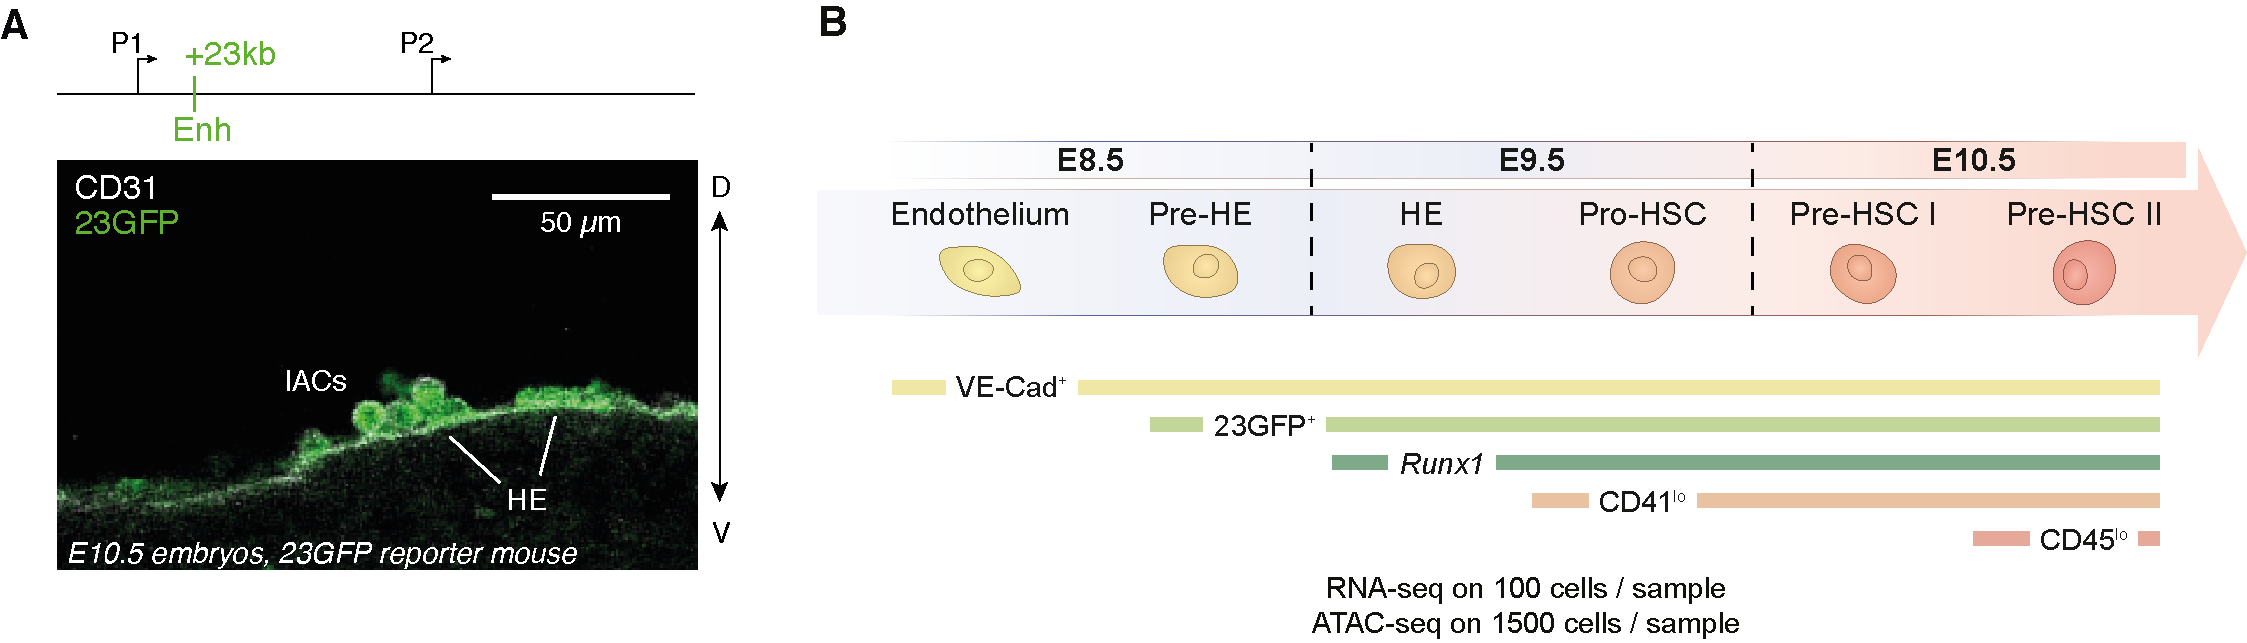
\includegraphics[width=\textwidth,height=\textheight,keepaspectratio]{figures/chapter3/ch3_overview.png}
    \caption[{Overview of profiled EHT populations.}]
    {\textbf{Overview of profiled EHT populations.} 
    \textbf{(A)} Top – Schematic of the \textit{Runx1} locus, with the +23 enhancer annotated in green. Bottom –  Immunofluorescence image of whole-mount 23GFP E10.5 AGM, showing a single 2.5 $\mu$m slice. 23GFP marked HE and IACs. 
    \textbf{(B)} Schematic of EHT cell populations sorted from E8.5, E9.5 and E10.5 mouse embryos, that were profiled by RNA-seq and ATAC-seq. Bars indicate population sort markers. Populations were first gated on Ter119\uneg{}. RNA-seq \textit{n} = 3 (pre-HE = 4) and ATAC-seq \textit{n} = 4 (pro-HSC = 3). 
    \textit{RNA-seq and ATAC-seq data were generated by previous members of the de Bruijn lab (G. Swiers and L.Greder, respectively) and were used in analyses and GRN construction performed by me.}
    }
    \label{fig:ch3_overview}
\end{figure}

To investigate the regulatory logic driving EHT I used data generated previously in the de Bruijn lab, namely transcription profiling and chromatin accessibility of bulk populations from the PAS/AGM + VU of E8.5 to E10.5 mouse embryos (Fig. \ref{fig:ch3_overview}B, Appendix \ref{fig:app_eht-sort-gates}A). These populations include E8.5 endothelial cells (EC, Ter119\uneg{}VECad\upos{}CD41\uneg{}CD45\uneg{}23GFP\uneg{}) and pre-HE (Ter119\uneg{}VECad\upos{}CD41\uneg{}CD45\uneg{}23GFP\upos{}), E9.5 HE (Ter119\uneg{}VECad\upos{}\-CD41\uneg{}CD45\uneg{}23GFP\upos{}) and pro-HSC (Ter119\uneg{}VECad\upos{}CD41\upos{}CD45\uneg{}), and E10.5 pre-HSC I (Ter119\uneg{}VECad\upos{}\-CD41\upos{}CD45\uneg{}) and pre-HSC II (Ter119\uneg{}VECad\upos{}CD41\upos{}CD45\upos{}). Sort panels for these populations did not include CD43, so the population indicated as 'pro-HSC' contains both pro-HSC (CD43\uneg{}, \cite{rybtsov_tracing_2014}) and blood progenitors (CD43\upos{}). E9.5 Ter119\uneg{}VECad\upos{}CD41\upos{}CD45\uneg{} PAS cells contain 80.3 \textpm 4.8\% CD43\upos{} haematopoietic progenitors (Appendix \ref{fig:app_eht-sort-gates}B).

Following pre-processing and mapping, reads were found to have high levels of PCR duplication (RNA-seq: 28\% - 72.7\% PCR duplication, with mean of 49.5\%. ATAC-seq: 58.3\% - 89\% PCR duplication, with mean of 78.5\%), and after PCR duplicate removal mapping was successful (Appendix \ref{fig:app_eht-qc}). Low-expressing genes were removed from the RNA-seq data (see methods section \ref{ch2:rna-analysis}, p.\pageref{ch2:rna-analysis}), before pre-processing with EdgeR \citep{robinson_edger:_2010}. Peak-calls were generated from individual ATAC-seq samples, and peaks overlapping in at least two replicates were retained, in order to discard low-quality peak calls. ATAC-seq signal was quantified over these robust peaks to create a peak read count table, and as with the RNA-seq data low count peaks were discarded (see methods section \ref{ch2:chip-atac-analysis}, p.\pageref{ch2:chip-atac-analysis}). 

\subsection[Different EHT expression signatures drive differentiation, morphological, and signalling processes]{\label{ch3:profiling}Different EHT expression signatures drive\\differentiation, morphological, and signalling\\processes}

\begin{figure}[!b]
    \centering
    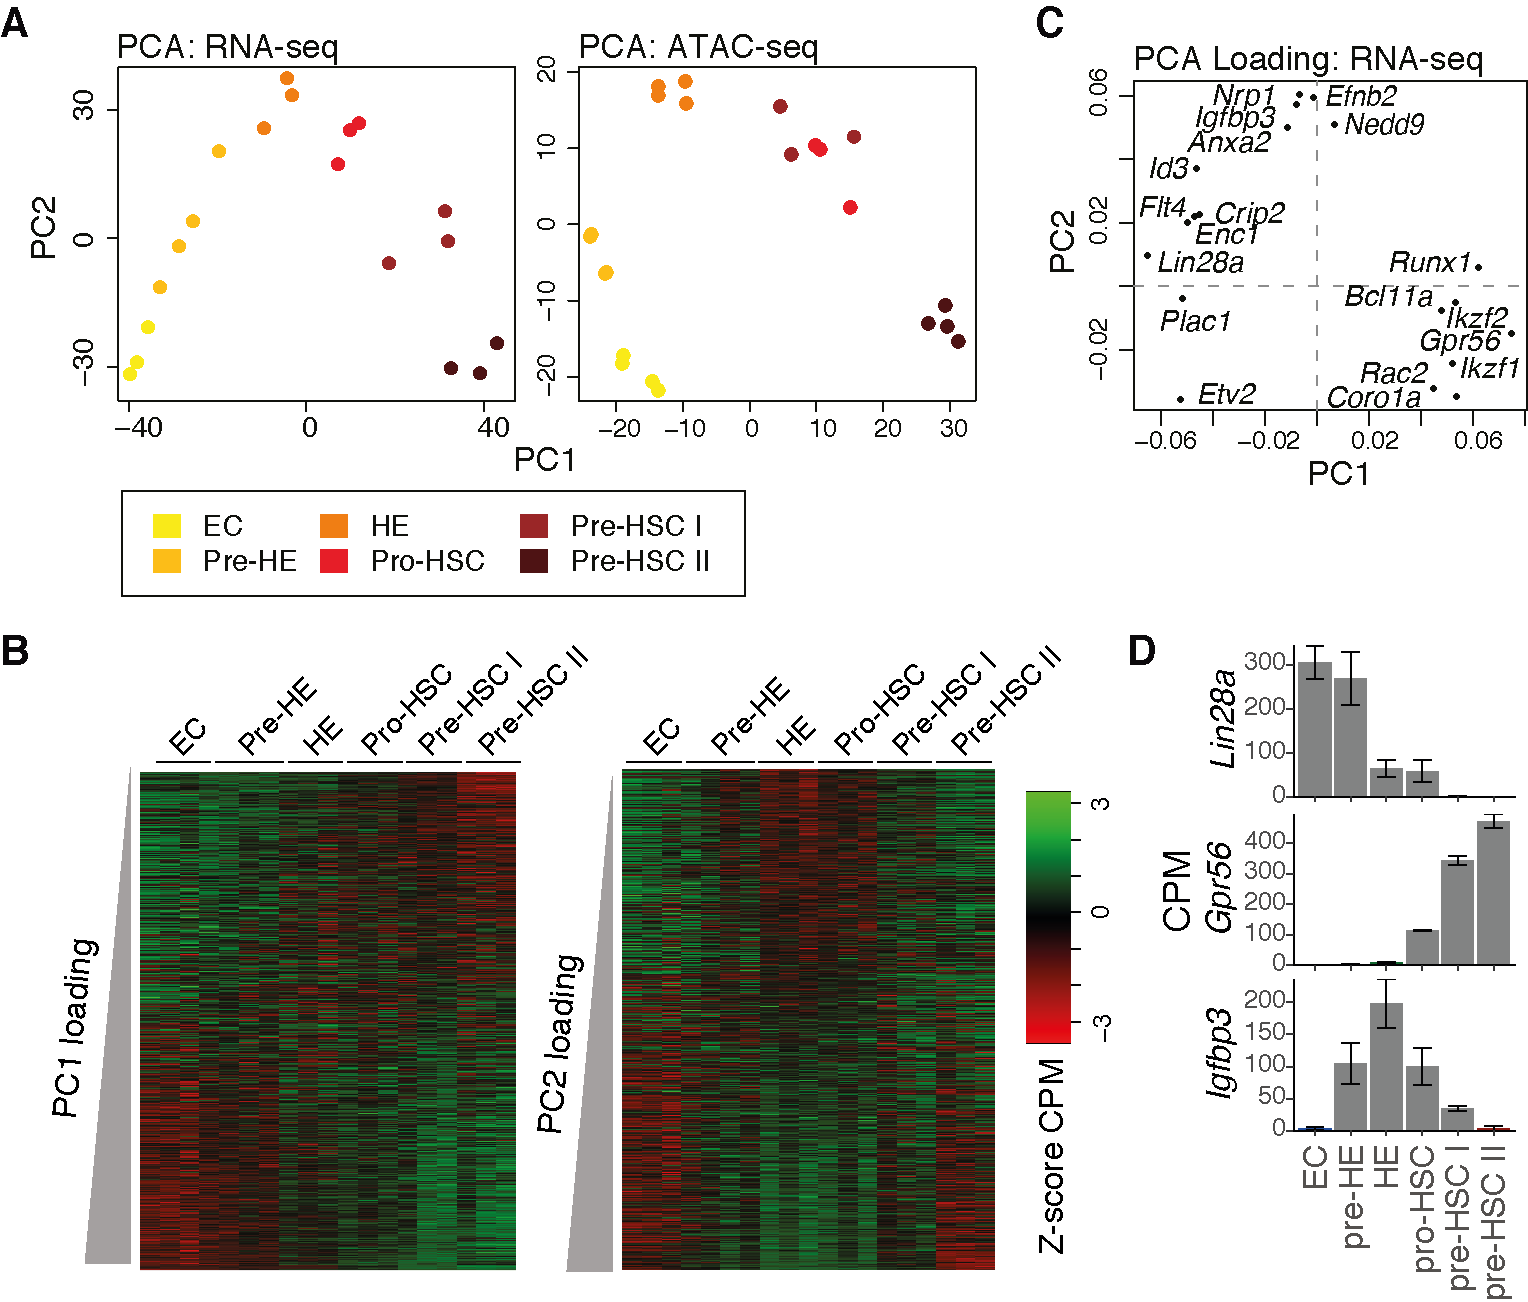
\includegraphics[width=\textwidth,height=\textheight,keepaspectratio]{figures/chapter3/ch3_pca.png}
    \caption[{EHT principal components define switch and transient gene regulation.}]
    {\textbf{EHT principal components define switch and transient gene regulation.} 
    \textbf{(A)} PCA plots of RNA-seq (left) and ATAC-seq (right) samples that describe the EHT transition. ANOVA DEG and DAEs used as input. 
    \textbf{(B)} Heatmap of RNA-seq gene expression (Log\textsubscript{2} CPM) ordered by PCA loading contribution to PC1 (left) and PC2 (right).
    \textbf{(C)} Top PC1+, PC1-, and PC2+ loadings relating to the RNA-seq PCA shown in A-B.
    \textbf{(D)} Average gene expression (CPM) plots for strong PC1 and PC2 loading genes. Error bars represent standard error of the mean; \textit{n} = 3; \textit{n} = 4 for pre-HE.
    }
    \label{fig:ch3_pca}
\end{figure}

To explore gene regulation in EHT, I first analysed general gene expression and chromatin accessibility profiles. As pairwise analysis between populations does not incorporate changes across the whole EHT process, I instead performed an ANOVA-like test in EdgeR \citep{robinson_edger:_2010} to extract differentially expressed genes (DEGs) from the RNA-seq data, and differentially accessible elements (DAEs) from the ATAC-seq data. This method tests for changes between any populations, and therefore identifies gene expression and ATAC accessibility generally associated with EHT. ANOVA tests identified 5892 DEGs in the RNA-seq data, and 17969 DAEs in the ATAC-seq data. 

PCA of the DEGs and DAEs clustered replicates together (Fig. \ref{fig:ch3_pca}A). The PC1 axis in both RNA-seq and ATAC-seq datasets represents a sequential progression of EHT. PC2 instead describes a transient activation or suppression of transcription, where expression peaks or troughs in HE/pro-HSC and returns to baseline levels in pre-HSCs (Fig. \ref{fig:ch3_pca}B). For example, \textit{Lin28a} is PC1- associated with high EC expression and is known to negatively regulate haematopoiesis \citep{chaudhuri_oncomir_2012}, while \textit{Gpr56} is PC1+ associated with high pre-HSC expression and is required for HSC generation \citep{solaimani_kartalaei_whole-transcriptome_2015} (Fig. \ref{fig:ch3_pca}C-D). \textit{Igfbp3} is PC2+ associated and transiently regulated with peak expression in HE (Fig. \ref{fig:ch3_pca}C-D), and is implicated in a range of pathways \citep{baxter_insulin-like_2013} but has not previously been implicated in EHT. PC1 loadings can be considered to reflect genes that switch on or off, while PC2 loadings represent transient regulation.

To properly categorise these DEGs and DAEs into different patterns, the RNA-seq and ATAC-seq counts were clustered into five regulatory modules (RNA1-5 and ATAC1-5, Fig. \ref{fig:ch3_clusters}A-B). The modules represent transient decrease (RNA1/ATAC1) or increase (RNA3/ATAC3) in RNA-seq and ATAC-seq counts, an endothelial bias (RNA2/ATAC2), early haematopoietic commitment (upregulation in HE/pro-HSC, RNA4/ATAC4), and late haematopoietic commitment (upregulation in pre-HSC I/II, RNA5/ATAC5). It is striking that similar patterns are observed between RNA-seq and ATAC-seq datasets. Clusters have been labelled to represent similar patterns between the datasets, such as RNA2 and ATAC2, both of which are downregulated over EHT. 

\begin{figure}[htbp]
    \centering
    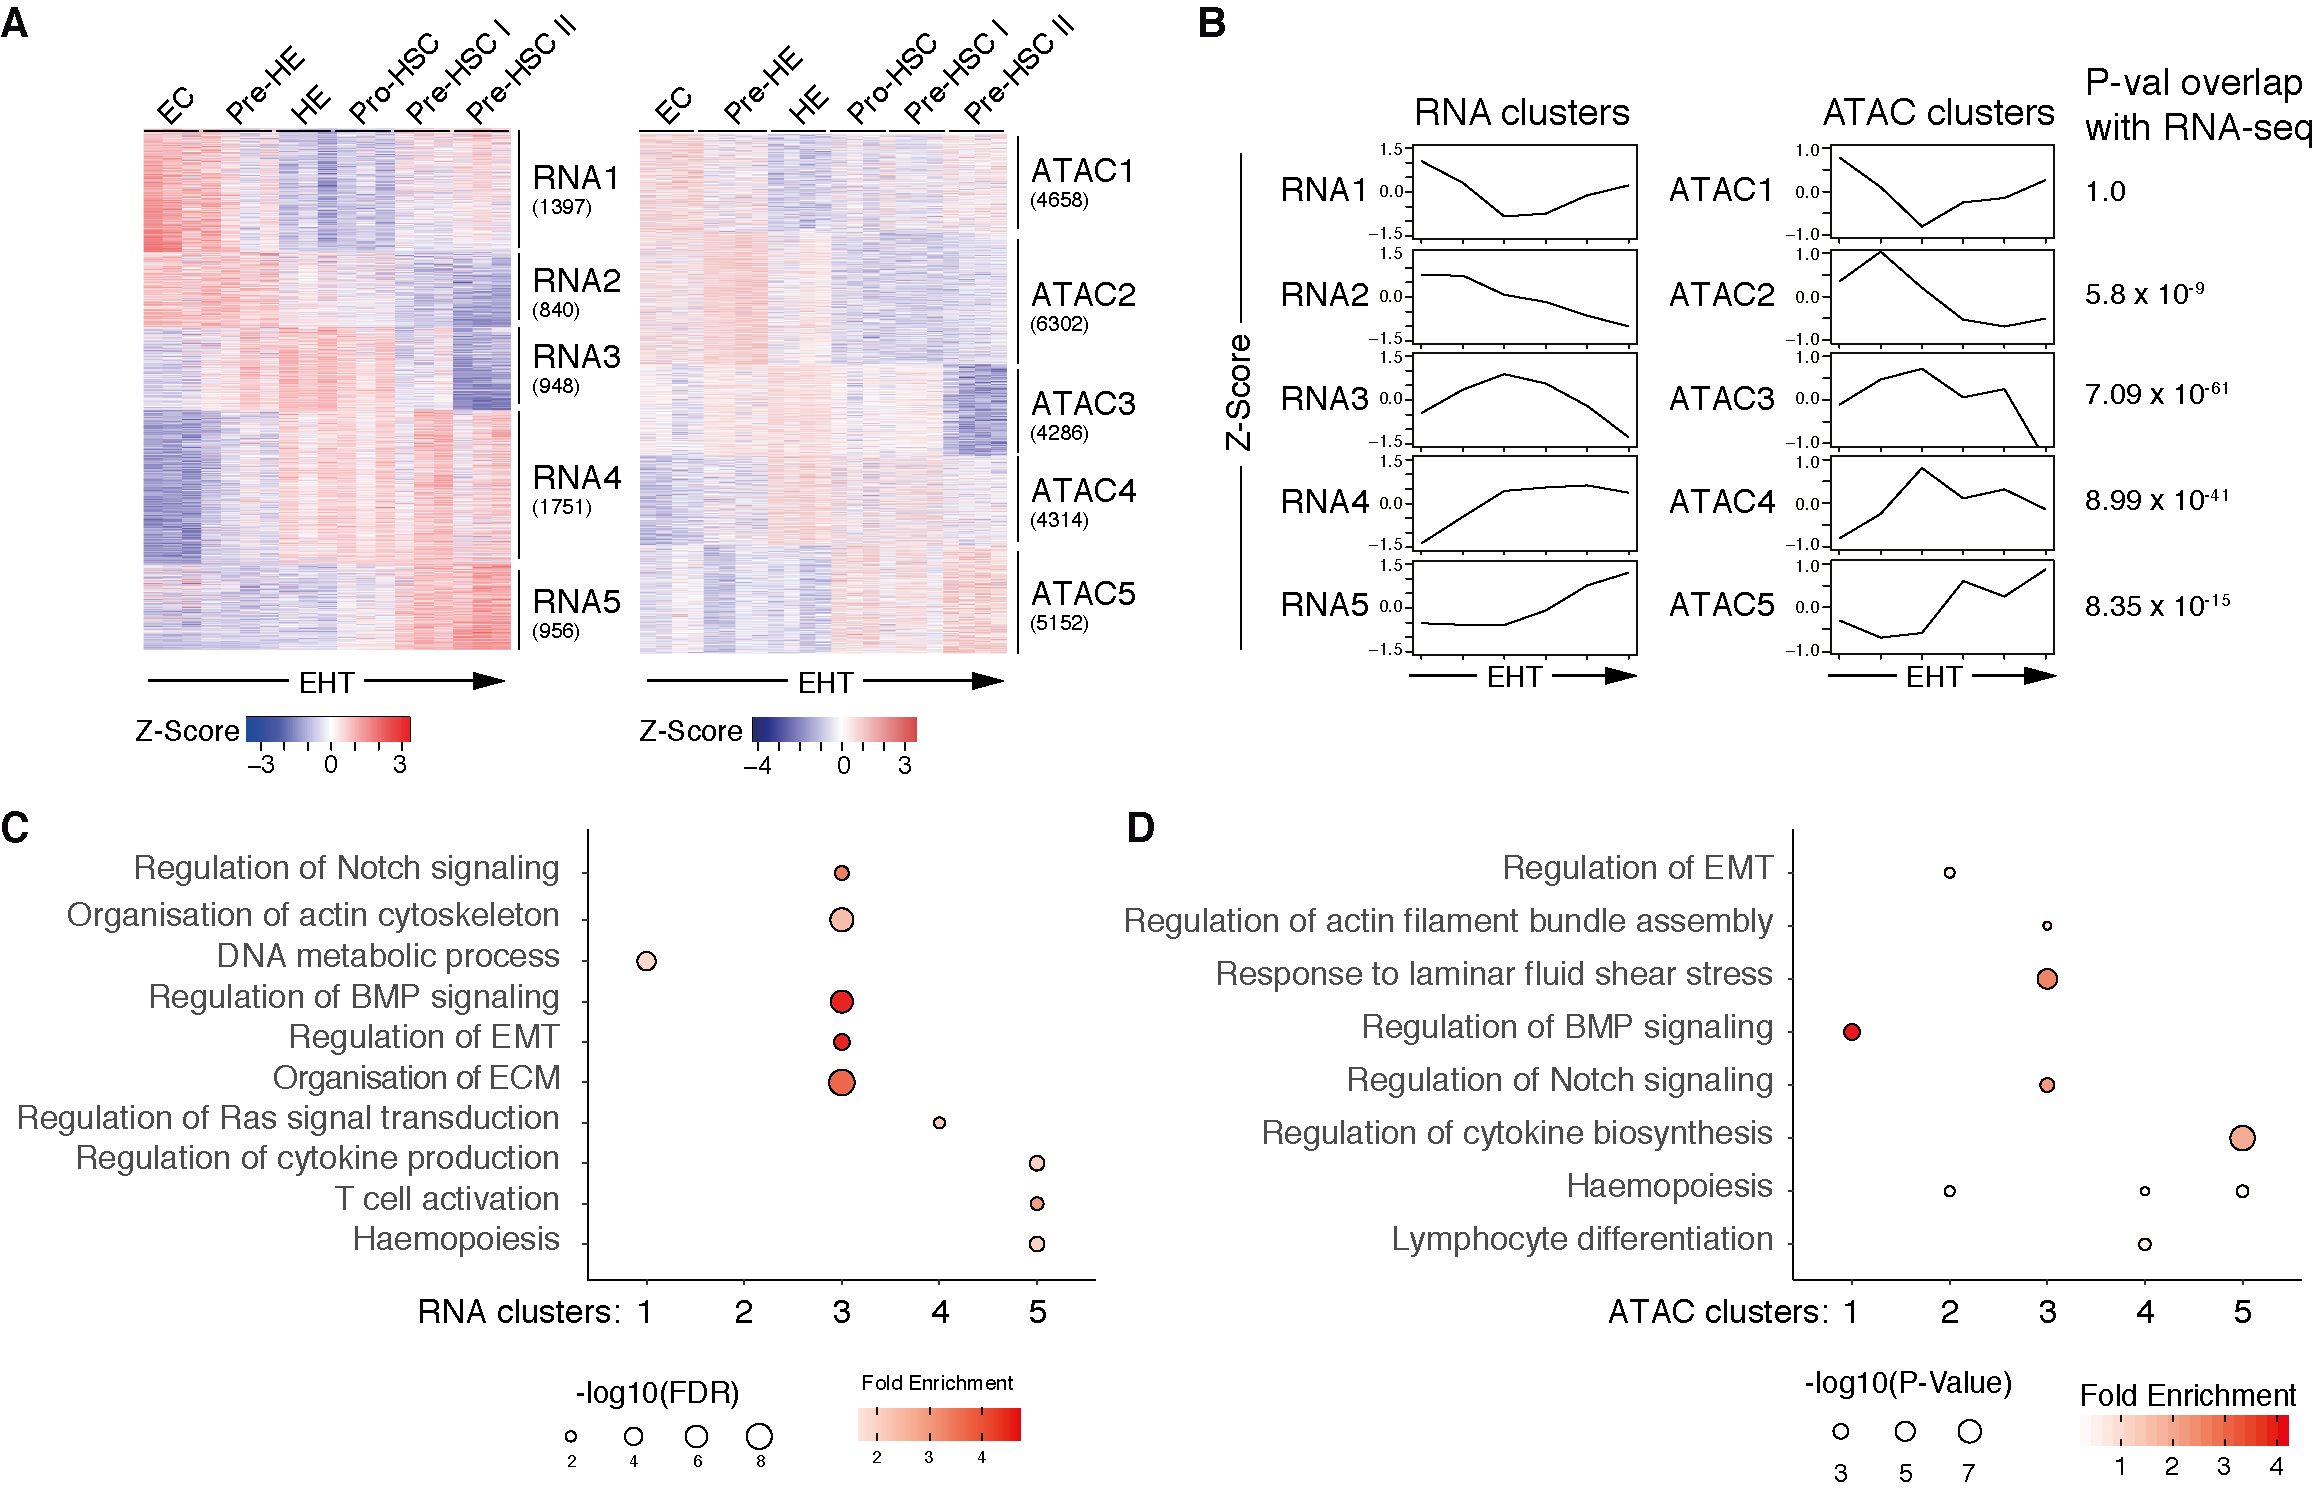
\includegraphics[width=\textwidth,height=\textheight,keepaspectratio]{figures/chapter3/ch3_clusters.png}
    \caption[{Transient regulation activates signalling and morphological changes while switches drive a haematopoietic phenotype.}]
    {\textbf{Transient regulation activates signalling and morphological changes while switches drive a haematopoietic phenotype.} 
    \textbf{(A)} Expression and accessibility heatmaps (Z-score Log\textsubscript{2} CPM) for RNA-seq DEGs  (left) and ATAC-seq DAEs (right). Expression grouped by hierarchical clustering, and accessibility by \textit{k}-means clustering. 
    \textbf{(B)} Average z-score Log\textsubscript{2} CPM of gene expression (left), or chromatin accessibility (right) by clusters as in A. Fishers exact test results comparing the overlap of corresponding RNA- and ATAC-seq clusters are shown on the side. 
    \textbf{(C-D)} GO biological process enrichment for modules RNA1-5 (C) and ATAC1-5 (D). Only significant data points shown (P $\leq$ 0.05).
    }
    \label{fig:ch3_clusters}
\end{figure}

As enhancer and promoter activity should drive gene expression changes it is expected that ATAC-seq peaks would be associated with genes within the same module, such as ATAC2 accessible elements linked to RNA2 genes. To test this hypothesis, I annotated each DAE to the closest DEG to associate enhancer and promoter elements to the corresponding gene. I then performed Fisher's exact tests to determine the significance of overlap between genes in RNA1-5 and genes linked to accessible elements in corresponding ATAC1-5 modules (Fig. \ref{fig:ch3_clusters}B). Each corresponding RNA-seq and ATAC-seq module, other than RNA1 and ATAC1, was significantly associated with each other, supporting the hypothesis that differential enhancer and promoter accessibility is driving gene expression changes.

These modules describe a range of dynamic profiles across EHT, though it is unclear whether clustering the data has functional relevance. To determine whether these modules drive specific programs, I performed gene ontology (GO) enrichment analyses (Fig. \ref{fig:ch3_clusters}C-D). Transiently activated genes (RNA3/ATAC3) are associated with Notch and BMP signalling, and processes that underpin morphological changes and migration, including epithelial-to-mesenchyme transition (EMT) and actin cytoskeleton organisation (Fig. \ref{fig:ch3_clusters}C-D). Late haematopoietic commitment (RNA5/ATAC5) is instead enriched for terms related to cytokine production, haematopoiesis, and T cell activation, corresponding with a differentiation program. This breakdown of regulatory patterns highlights the complex regulation over EHT and begins to categorise distinct regulatory programs. In particular, transient activation is associated with signalling and morphological changes that may drive the budding process during EHT.

\subsection{\label{ch3:cd109}Transition-specific regulation}

EHT is controlled through specific sequential transitions between cell types. Therefore, an initial characterisation of RNA-seq and ATAC-seq changes at these transitions is important to understand. In particular, understanding the difference between E8.5 ECs and E8.5 pre-HE can identify key genes that distinguish this pre-HE population. To identify specific regulatory changes characterising cell type transitions I performed pairwise differential analyses between sequential EHT populations. As with the ANOVA analysis, DAEs were associated with the closest DEG promoter. As it is expected for changes in chromatin accessibility to reflect gene expression, I examined the relationship between RNA-seq and ATAC-seq logFC between transitions. Changes in chromatin accessibility and gene expression are generally concordant, such as with the EC to pre-HE transition where 79\% of opening chromatin elements associate with upregulated genes (Fig. \ref{fig:ch3_stage-enhs}A). This concordance is not present in all transitions, such as the pre-HE to HE transition where 33\% of closing elements are associated with increasing expression (Fig. \ref{fig:ch3_stage-enhs}A). This could be due to incorrect assignment of elements to gene promoters, or reflect silencers or non-regulatory elements.

\begin{figure}[t]
    \centering
    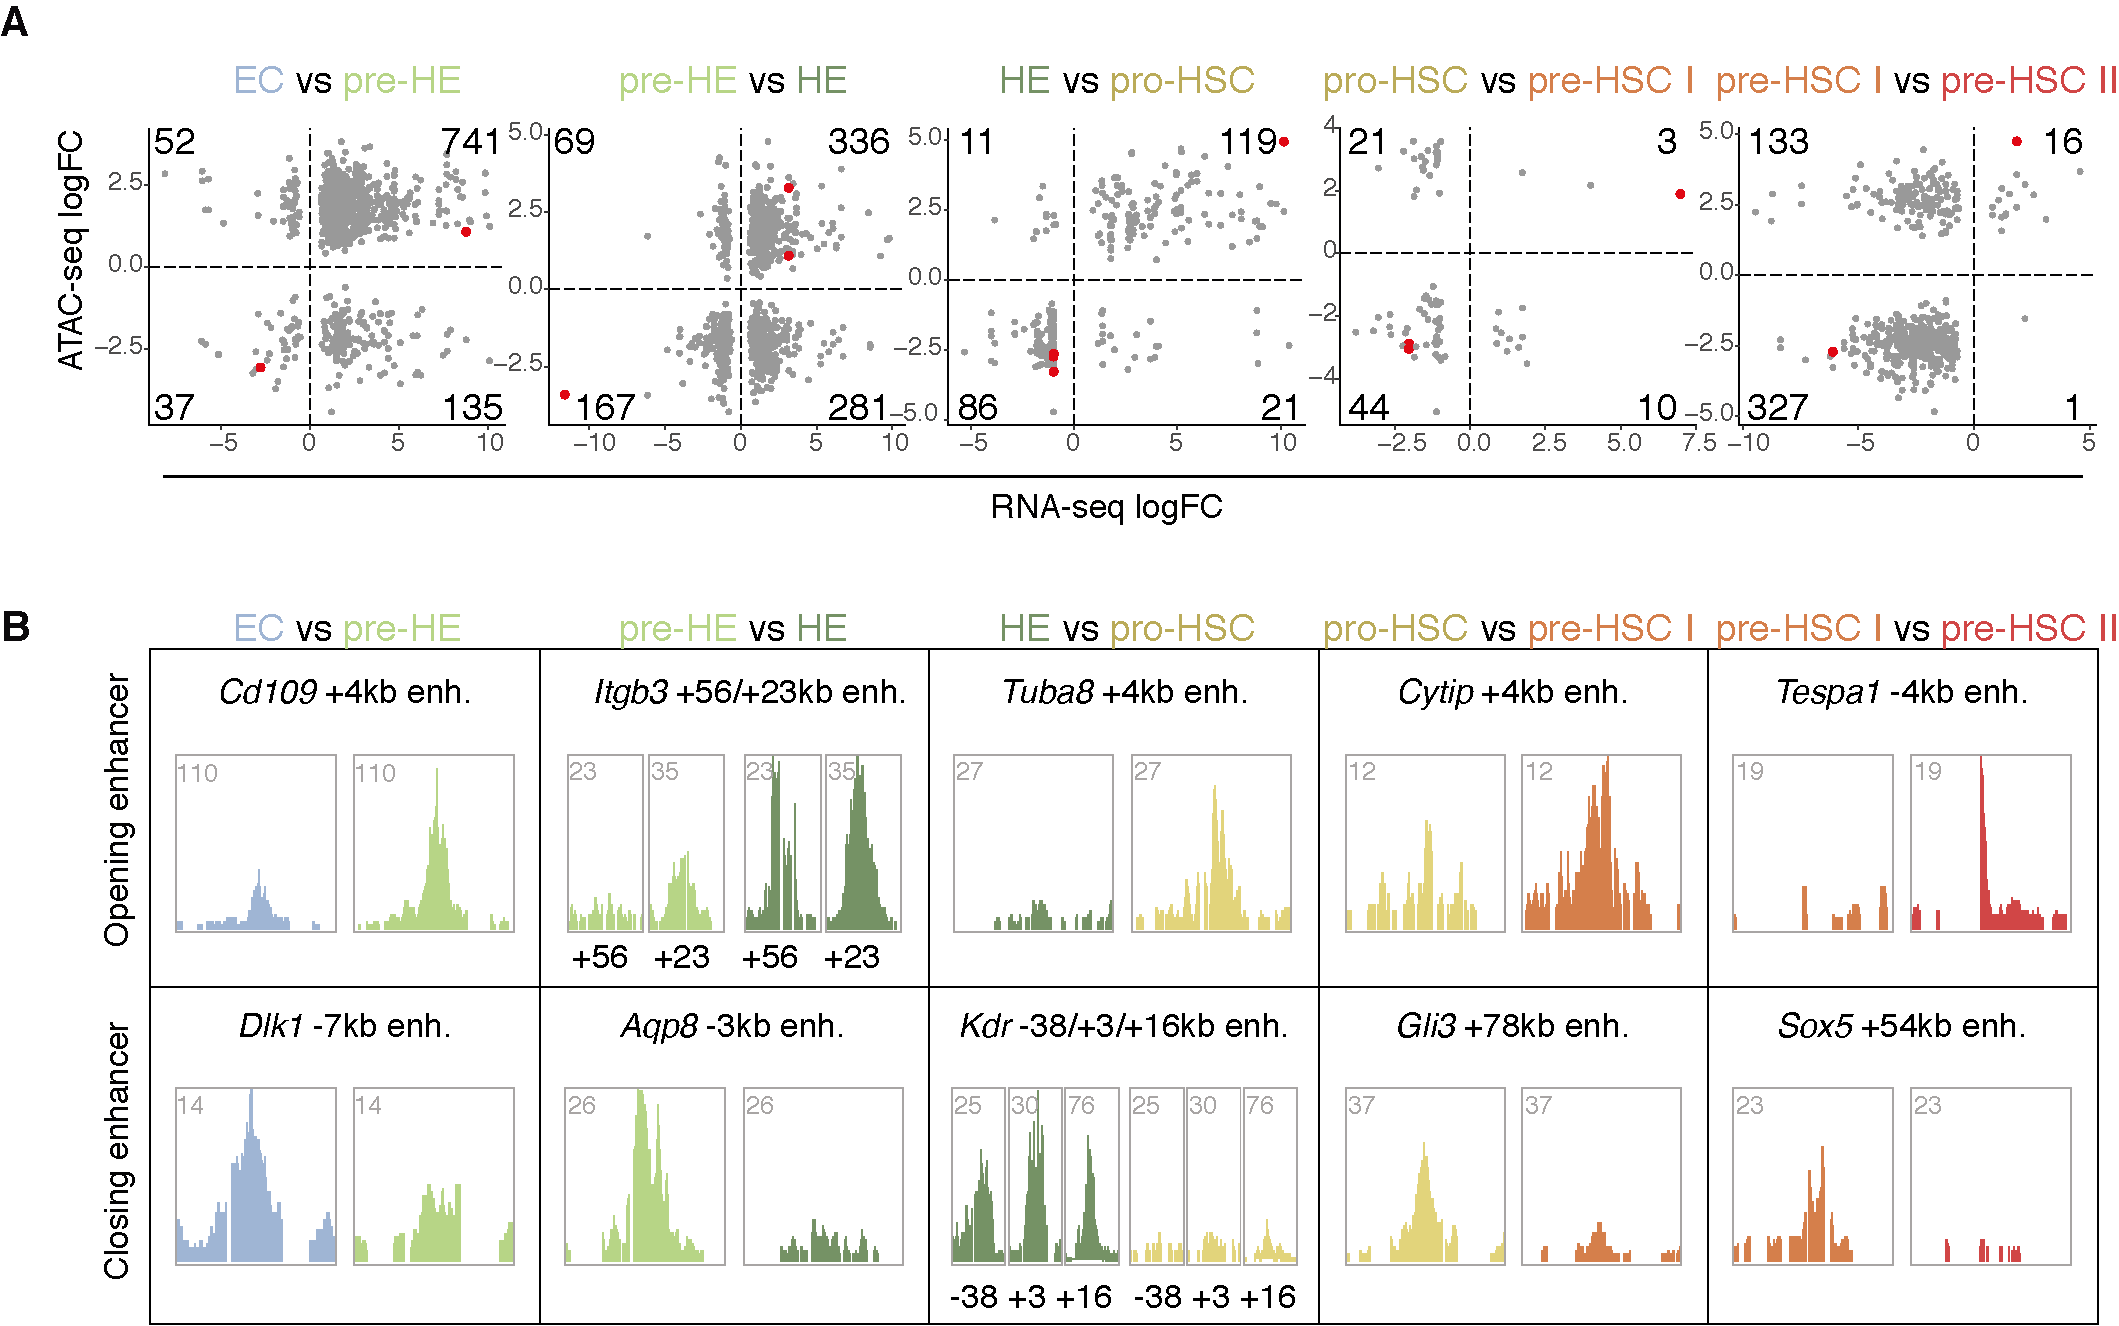
\includegraphics[width=\textwidth,height=\textheight,keepaspectratio]{figures/chapter3/ch3_stage-enhs.png}
    \caption[{Analysis of enhancer-promoter pairs suggests stage-specific epigenetic regulation.}]
    {\textbf{Analysis of enhancer-promoter pairs suggests stage-specific epigenetic regulation.} 
    \textbf{(A)} Relationship between RNA- and ATAC-seq logFC at significant pairwise comparisons. Each data point represents an accessible element paired with a gene (as defined by closest DEG promoter to the element). Only non-promoter elements are shown (distance > 1kb from TSS). High logFC genes that have relevance to EHT based on existing literature were highlighted red, and examined in B.  
    \textbf{(B)} ATAC-seq tracks for DAEs, as highlighted in A. Sample replicates were combined into a single track. Values indicate track height. Opening elements: logFC > 0 and FDR < 0.05, closing elements: logFC < 0 and FDR < 0.05. 
    }
    \label{fig:ch3_stage-enhs}
\end{figure}


To find regulatory elements associated with cell type transitions, I focused on strongly differential genes and accessible elements (Fig. \ref{fig:ch3_stage-enhs}B). I selected example genes and elements displaying among the highest or lowest logFC values between transitions, that were relevant to EHT based on known literature. The EC to pre-HE transition, marking the earliest initiation of EHT signalling, shows strong upregulation of \textit{Cd109} expression and opening of a +4kb element, and a decrease in \textit{Dlk1} and a -7kb element (Fig. \ref{fig:ch3_stage-enhs}B). CD109 is known to be expressed in CD34+ bone marrow cells, marking haematopoietic populations \citep{murray_cd109_1999} (though decreases in expression with HSC maturation in the embryo, see Fig. \ref{fig:ch3_cd109}B). Dlk1 is a known negative regulator of EHT normally expressed in the surrounding AGM niche \citep{mirshekar-syahkal_dlk1_2013}. Genes upregulated in the pre-HE to HE transition include \textit{Itgb3} (CD61) which is a known marker of HE \citep{huang_generation_2016}. HE to pro-HE is characterised by deactivation of \textit{Kdr} (Flk1), a receptor marking vascular endothelium \citep{millauer_high_1993}, and increased \textit{Tuba8}, a tubulin \citep{stanchi_tuba8_2000}, which reflects a loss of endothelial identity and cytoskeletal changes, respectively. Few genes are upregulated in pro-HSC to pre-HSC I, and pre-HSC I to II transitions, with the majority of genes being downregulated. Among downregulated genes in these transitions are several key TFs, including \textit{Gli3}, which is known to modulate hedgehog signalling \citep{chaudhry_gli3_2017}, and \textit{Sox5} which modulates BMP signalling \citep{nordin_sox5_2014}.

\begin{figure}[t]
    \centering
    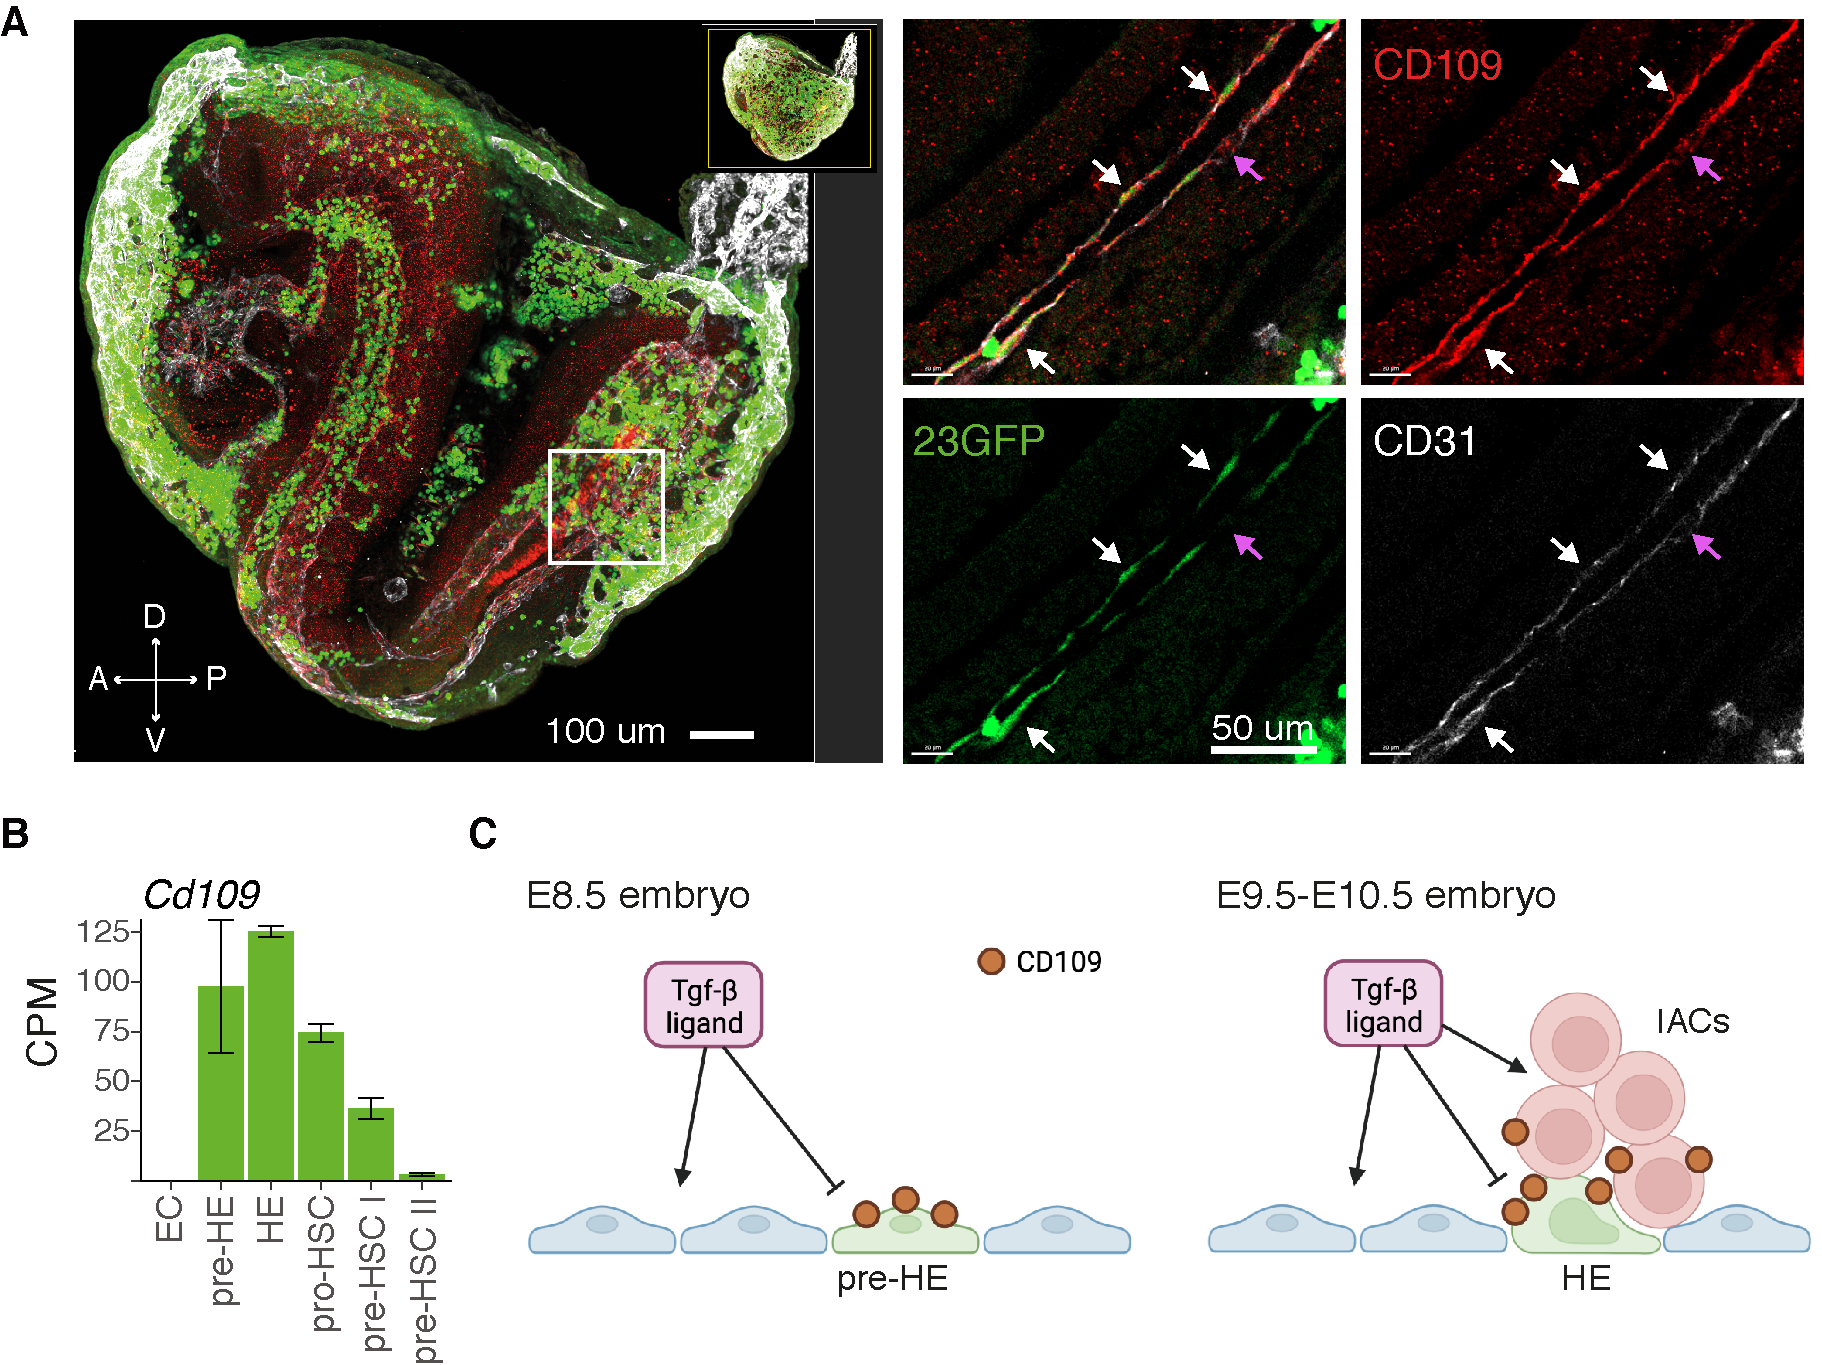
\includegraphics[width=\textwidth,height=\textheight,keepaspectratio]{figures/chapter3/ch3_cd109.png}
    \caption[{\textit{CD109} expression and protein localisation in E8.5 embryos.}]
    {\textbf{\textit{CD109} expression and protein localisation in E8.5 embryos.} 
    \textbf{(A)} Confocal whole‐mount immunofluorescence images of an E8.5 (5 somite pairs) 23GFP embryo. Left panel shows maximum intensity projection of paired dorsal aorta (225 $\mu$m thick Z‐stack), with maximum project of whole embryo shown at the top right (340 $\mu$m thick Z‐stack). Square box highlights region of interest. Right panels show a single 5 $\mu$m thick z-stack slice of the region of interest. White arrows indicate examples of CD109 and 23GFP overlap in endothelium, and purple arrows indicate an example of 23GFP- endothelium with low CD109. 
    \textbf{(B)} Gene expression (CPM) for \textit{Cd109} in bulk RNA-seq data. Error bars represent standard error of the mean; \textit{n} = 3; \textit{n} = 4 for pre-HE. 
    \textbf{(C)} Schematic illustrating hypothesised activity of TGF-$\beta$, on the basis of CD109 repressing TGF-$\beta$ receptor activation. \textit{Panel C created with BioRender.com.} 
    }
    \label{fig:ch3_cd109}
\end{figure}

The high expression of \textit{CD109} in pre-HE is of particular interest, as CD109 is known to attenuate TGF-$\beta$ signalling \citep{mii_cd109_2019}. \textit{Cd109} was expressed in E8.5 pre-HE, but not ECs, which was further validated by immunofluorescence imaging showing CD109 protein overlaps with 23GFP+ pre-HE in E8.5 embryos (Fig. \ref{fig:ch3_cd109}A-B). Additionally, \textit{Cd109} expression decreases as EHT progresses from pro-HSC to pre-HSC II (Fig. \ref{fig:ch3_cd109}B). Together, this data highlights that CD109 activity is enriched in pre-HE and HE over other EHT populations. As CD109 may repress TGF-$\beta$ activity, this suggests that the TGF-$\beta$ pathway is inactive specifically in pre-HE and HE, but maintains activity in E8.5 EC, and more mature pre-HSC populations (Fig. \ref{fig:ch3_cd109}C). Maintained TGF-$\beta$ activity in ECs is important, as the TGF-$\beta$ pathway is a regulator of EC proliferation \citep{lebrin_tgf-_2005, goumans_balancing_2002}. Further study is required to determine whether this CD109 enrichment is sufficient to impact TGF-$\beta$ signalling, and whether CD109 has an effect on EHT initiation or progression. 

\section{\label{ch3:grn}Generating, and characterising a GRN model of EHT}

\begin{figure}[t]
    \centering
    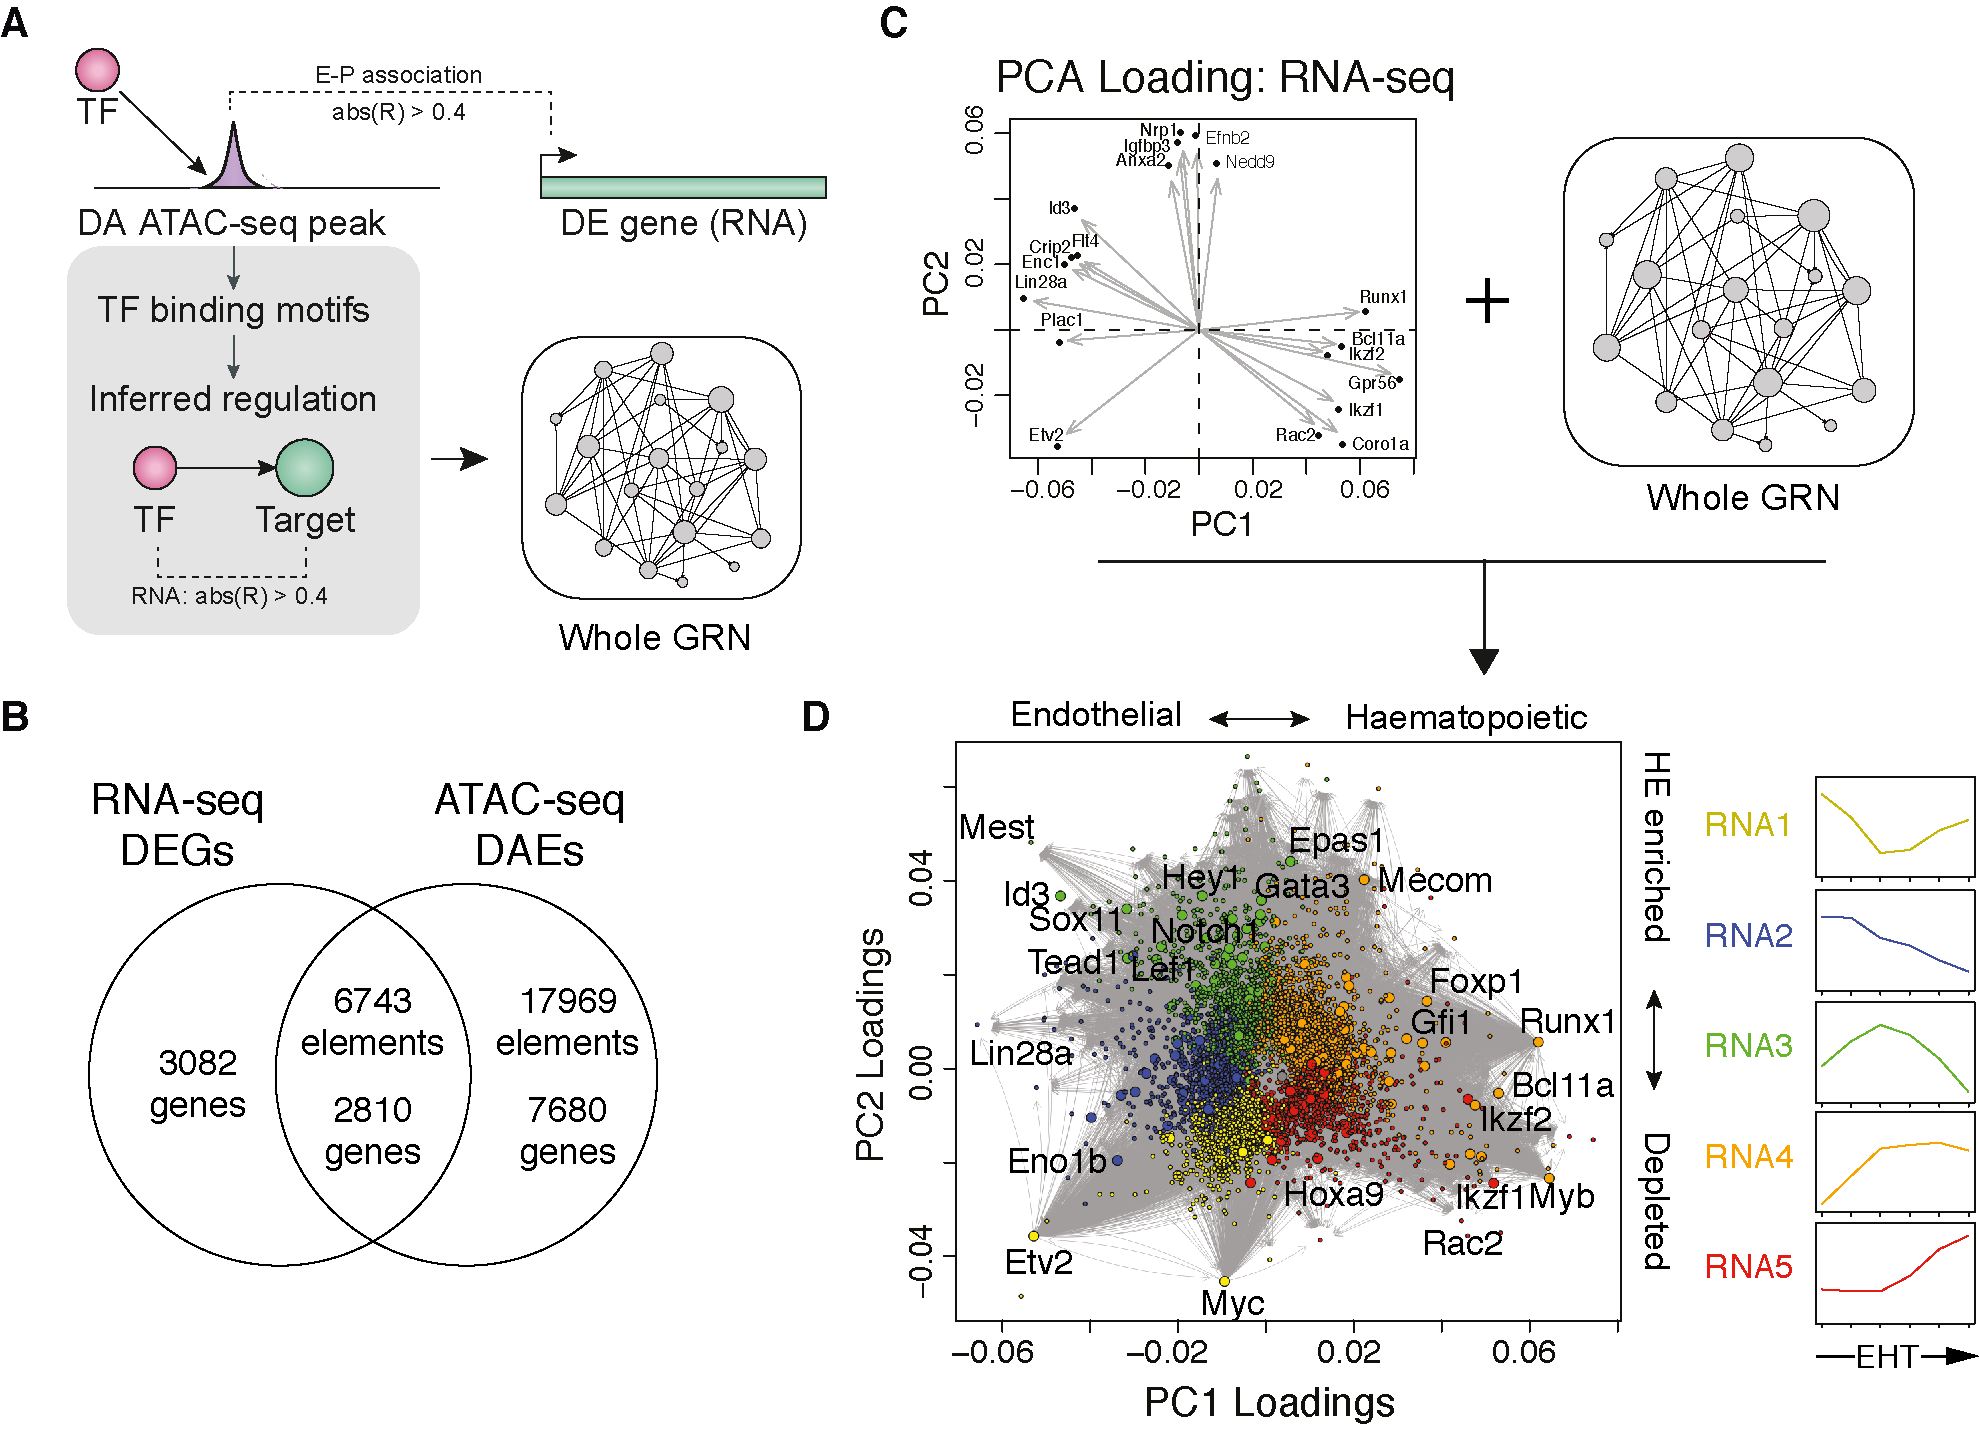
\includegraphics[width=\textwidth,height=\textheight,keepaspectratio]{figures/chapter3/ch3_eht-grn.png}
    \caption[{Constructing a GRN model of EHT.}]
    {\textbf{Constructing a GRN model of EHT.} 
    \textbf{(A)} Schematic outlining approach to generate the EHT GRN (methods section \ref{ch2:eht-grn}, p.\pageref{ch2:eht-grn}). 
    \textbf{(B)} Overlap of RNA-seq DEGs and genes in E-Ps at DAEs. 
    \textbf{(C)} Schematic illustrating approach to integrate RNA-seq PCA loadings (Fig. \ref{fig:ch3_pca}C) with the GRN model, to arrange the network nodes based on PCA loading coordinates (methods section \ref{ch2:eht-grn}, p.\pageref{ch2:eht-grn}). 
    \textbf{(D)} Visualization of the EHT network embedded in RNA PCA loading coordinates (Fig. \ref{fig:ch3_pca}C), as illustrated in C. Nodes are coloured according to RNA-seq module (Fig. \ref{fig:ch3_clusters}A-B). Module expression illustrated (right). All TF nodes are enlarged, with select TFs labelled.
    }
    \label{fig:ch3_eht-grn}
\end{figure}

To better understand the regulatory logic driving EHT, I constructed a GRN model using a multi-step approach to integrate RNA-seq and ATAC-seq profiles (Fig. \ref{fig:ch3_eht-grn}A, Appendix \ref{fig:app_eht-workflow}, methods section \ref{ch2:eht-grn}, p.\pageref{ch2:eht-grn}). Accessible regions were assigned to the closest active promoter, and those with strong correlation (> 0.4 or < -0.4) between ATAC-seq counts of the accessible element, and RNA-seq counts of the assigned promoter, were classified as enhancer-promoter associations (E-Ps). As both positive and negative correlation is incorporated, this definition of E-P also includes negative regulating elements (silencers). This definition of silencers has been used in \cite{cornejo-paramo_distal_2022}. While nearest promoter is not a robust definition, as enhancers can have low regulatory function or skip promoters to act on distal genes \citep{chepelev_characterization_2012}, the correlation filter enriches for valid regulatory interactions (as used in \cite{sheffield_patterns_2013, hariprakash_computational_2019}). To focus on dynamic regulation, only E-Ps connecting differential enhancers with differential expression were retained (2810 DEGs and 6743 associated DAEs, Fig. \ref{fig:ch3_eht-grn}B). Upstream regulators at enhancers and promoters were inferred by presence of TF binding motifs. To improve reliability, only high confidence motif matches were used (P < \xten{1}{-6}). Only robust interactions were retained, with strong RNA-seq correlation (> 0.4 or < -0.4) between the TF and predicted TF target. This established an integrated network of EHT regulatory interactions.

To interpret this model in the context of EHT, the network was embedded into RNA-seq PCA loading coordinates (Fig. \ref{fig:ch3_pca}C) and annotated by expression modules (Fig. \ref{fig:ch3_clusters}A). This stratified nodes based on expression profiles, describing EHT progression (PC1) and transiently expressed genes (PC2) (Fig. \ref{fig:ch3_eht-grn}C-D). For example, this clearly marks major nodes of the mature haematopoietic program (RNA4 and RNA5), including \textit{Gpr56}, \textit{Bcl11a}, \textit{Rac2}, and \textit{Myb}. The transient program (RNA3) was instead characterised by signalling associated genes, including \textit{Tead1}, \textit{Sox11}, \textit{Gata3}, and multiple Notch pathway genes. Together, this establishes an integrated model of EHT regulatory interactions, that organises the primary drivers of the five identified expression modules. 

\subsection{\label{ch3:centrality}Central regulators and targets of the EHT GRN}

To identify key regulators of the five expression modules, I calculated centrality measures to describe GRN nodes based on their connections within the network. Degree centrality is a measure of how many interactions are connected to a node (methods section \ref{ch2:centrality}, p.\pageref{ch2:centrality}), and in other systems has shown to correlate with gene essentiality \citep{hahn_comparative_2005, jeong_lethality_2001, koschutzki_centrality_2008}. Within the early haematopoietic commitment module (RNA4) the TFs with the highest degree centrality include Sp4, Smad3, and Klf4, in addition to the expected TFs Runx1, Gfi1, and PU.1 (\textit{Spi1}) (Fig. \ref{fig:ch3_centrality}A). Late haematopoietic commitment (RNA5) central nodes include Elf1, Nr1d2 and Ikzf1. TFs central to the transient module (RNA3) include Ets2, Nfib, Lef1 and Gata3/6. In addition to highly central TFs, genes with many accessible enhancers may indicate loci highly regulated during EHT (Fig. \ref{fig:ch3_centrality}B). \textit{Kdr} (Flk1) and \textit{Aplnr}, a marker of endothelium previously suggested to give rise to HE \citep{crosse_multi-layered_2020}, have many endothelium biased enhancers (ATAC2). Among transiently accessible enhancers \textit{Igfbp3} is associated with many accessible enhancers (Fig. \ref{fig:ch3_centrality}B) and drives HE identity (Fig. \ref{fig:ch3_pca}C-D). The central TFs \textit{Nfib} and \textit{Fli1} are also regulated by several transient enhancers. Among haematopoietic expression modules (RNA4 and RNA5) \textit{Ikzf1}, which is a highly central RNA5 TF (Fig. \ref{fig:ch3_centrality}A), has many accessible enhancers (ATAC5). The frequency of enhancers at these predicted key drivers of EHT, suggests that important factors are robustly regulated through multiple enhancers.

\begin{figure}[t]
    \centering
    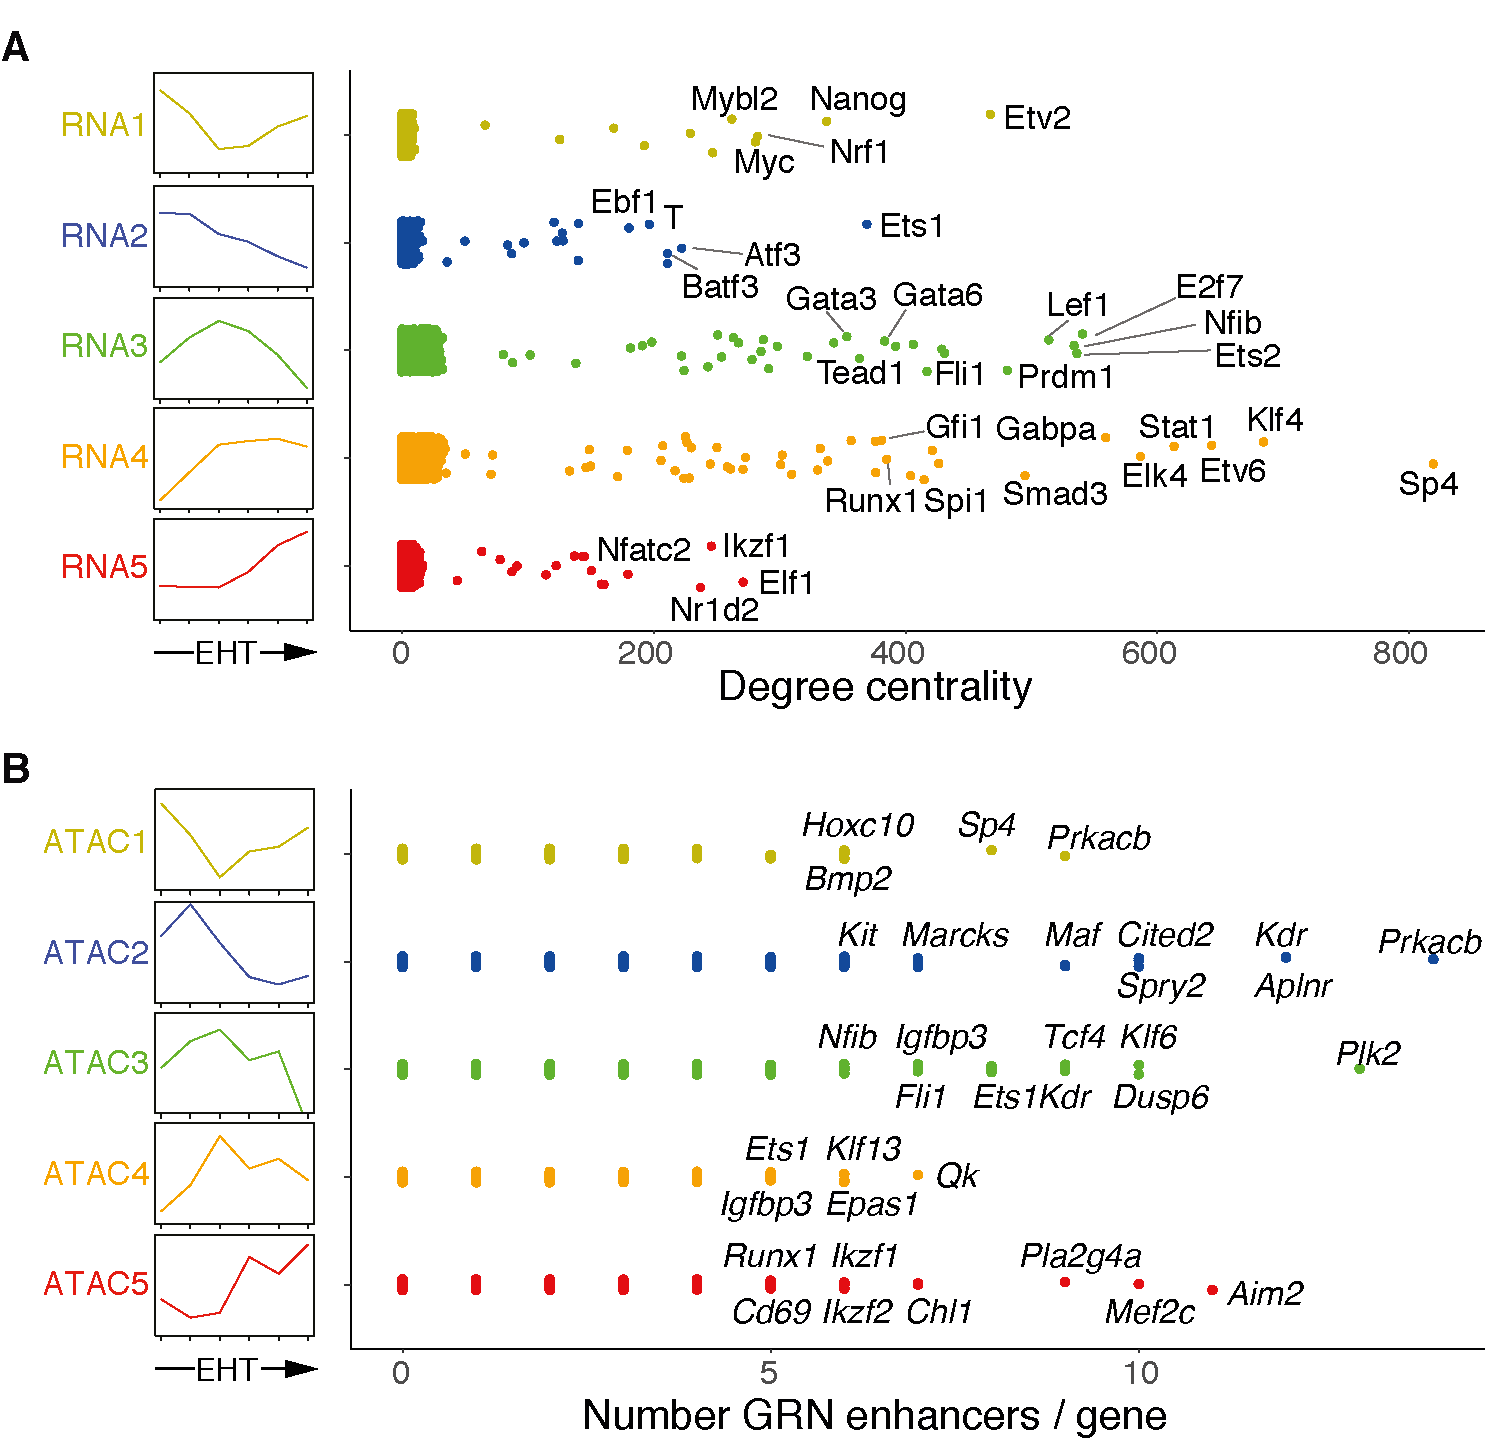
\includegraphics[width=\textwidth,height=\textheight,keepaspectratio]{figures/chapter3/ch3_centrality.png}
    \caption[{Centrality analysis predicts TF drivers of EHT modules.}]
    {\textbf{Centrality analysis predicts TF drivers of EHT modules.} 
    \textbf{(A)} Distribution of degree centrality of GRN nodes, stratified by RNA-seq expression clusters (RNA1-5). Select genes have been labelled to highlight top central regulators and key haematopoietic TFs. 
    \textbf{(B)} Number of enhancers linked to each gene, stratified by ATAC-seq accessibility clusters (ATAC1-5). Select genes shown to highlight example loci with many enhancers. 
    }
    \label{fig:ch3_centrality}
\end{figure}

\section{\label{ch3:runx1-context}\textit{Runx1} regulators and target genes}

As Runx1 is a critical regulator of EHT, it is important to understand its role in the GRN. To begin to investigate how Runx1 drives gene expression changes, it is important to understand the regulatory context of \textit{Runx1}. Specifically, I explored novel upstream regulators of \textit{Runx1}, and downstream targets coinciding with Runx1 activity.

\subsection{\label{ch3:runx1-landscape}Cis-regulatory landscape of the \textit{Runx1} locus}
% A caveat with this data is that the +23 enhancer is indistinguishable from the 23GFP enhancer reporter, which exists in a different genomic context and may explain low level accessibility seen in ECs.

\begin{figure}[!b]
    \centering
    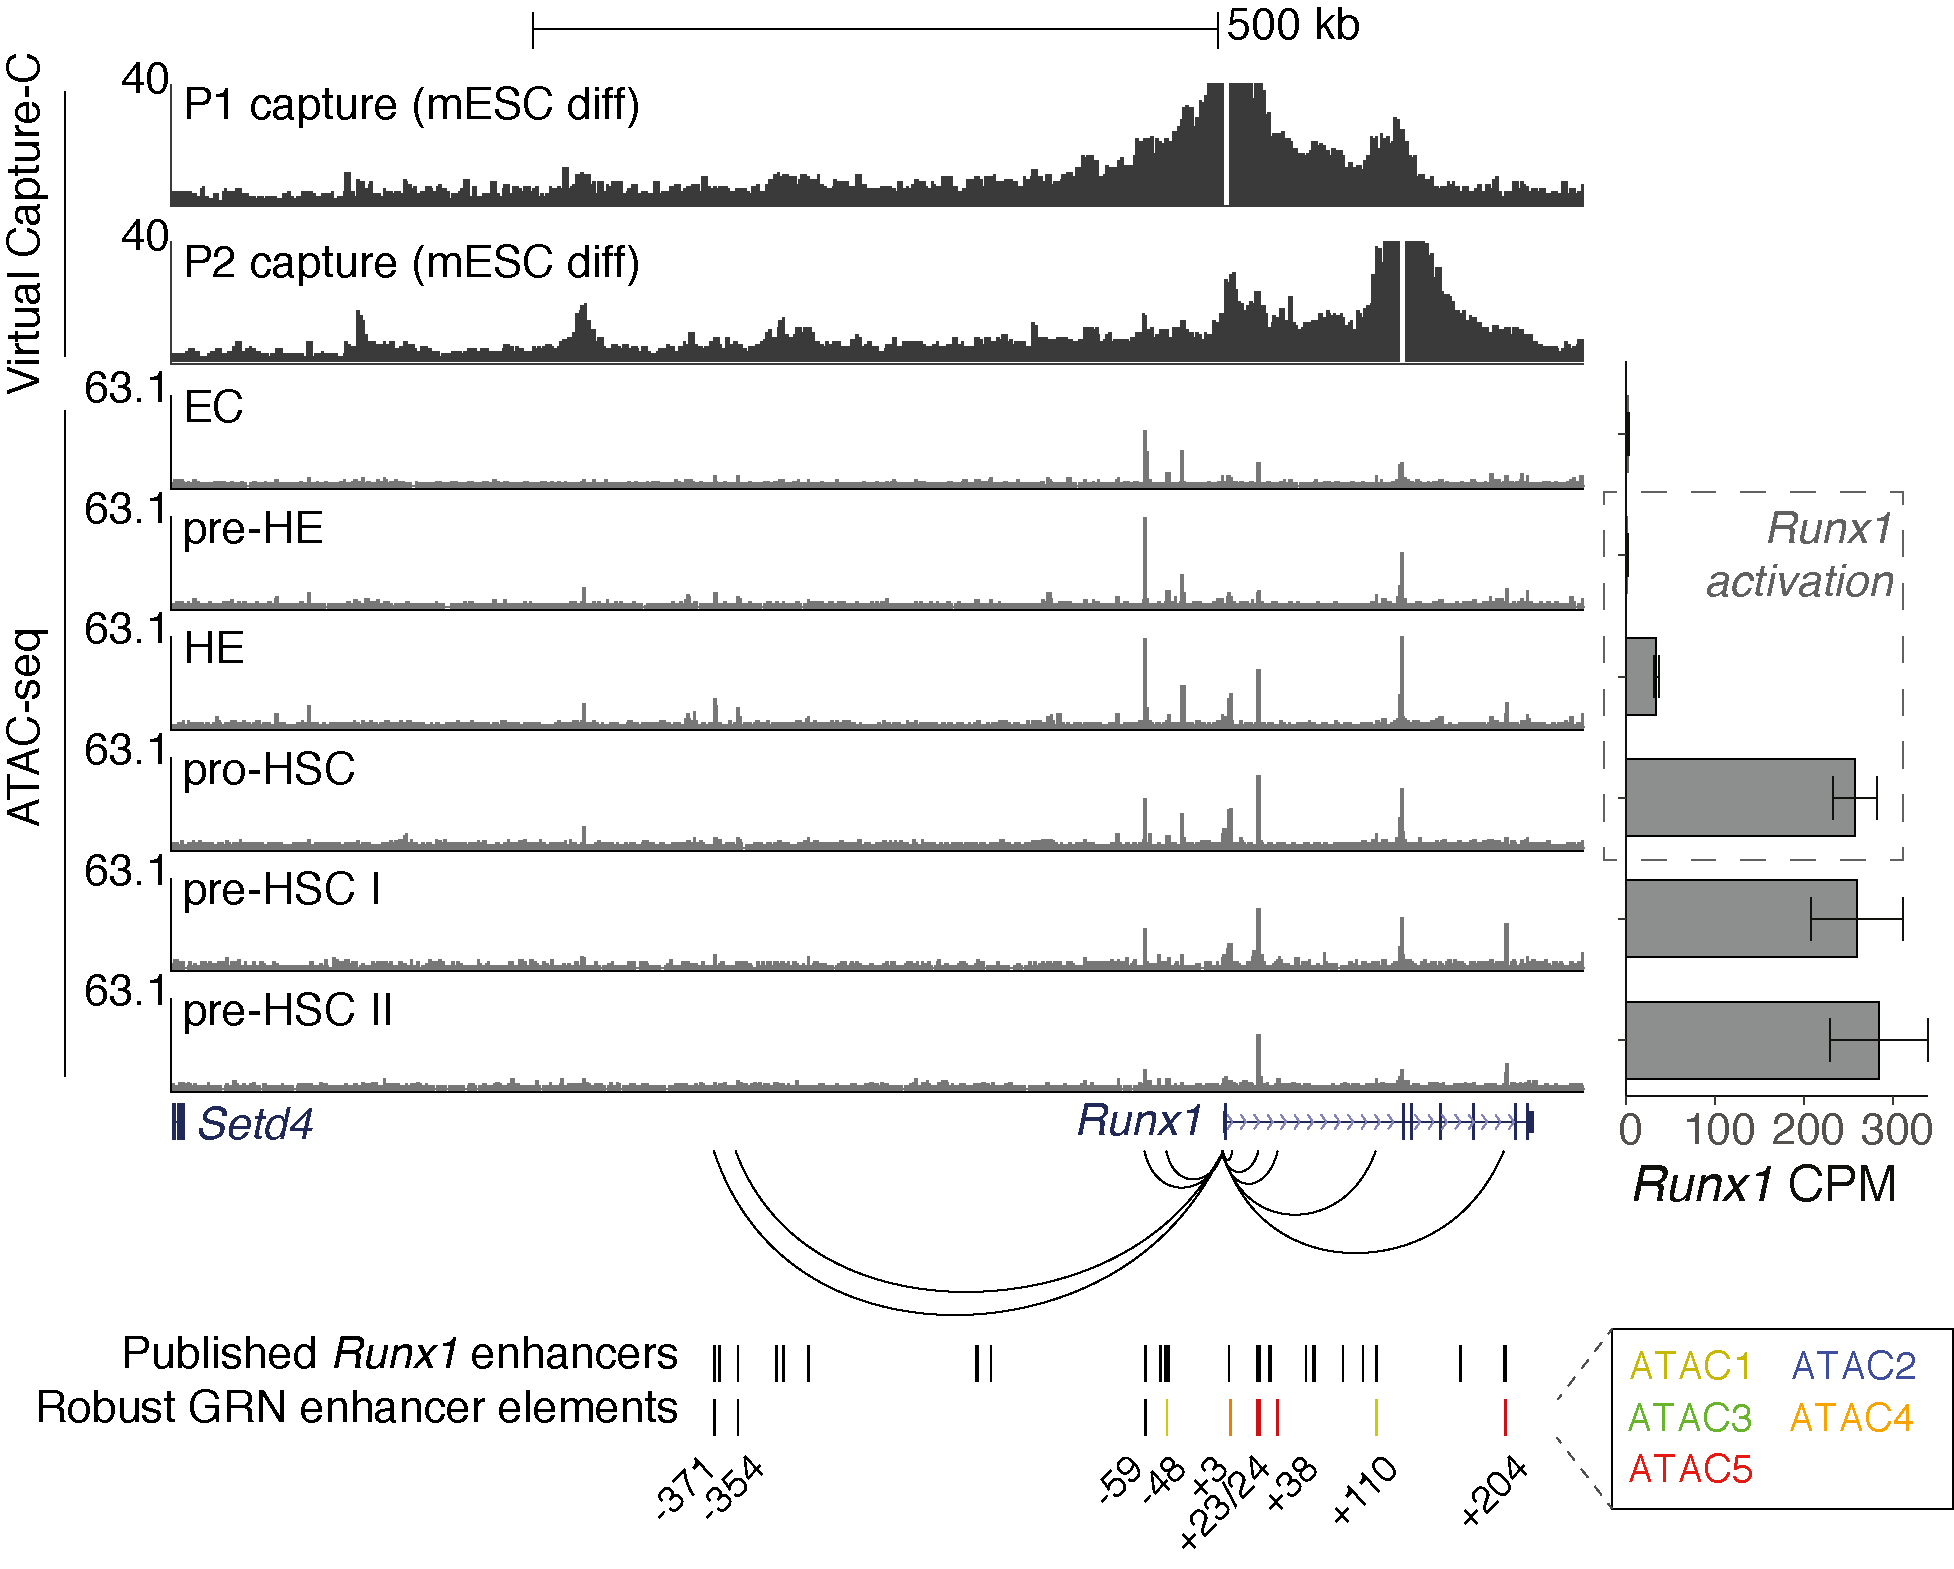
\includegraphics[width=\textwidth,height=\textheight,keepaspectratio]{figures/chapter3/ch3_runx1-regulation.png}
    \caption[{Chromatin accessibility profiles and predicted enhancers across the \textit{Runx1} locus.}]
    {\textbf{Chromatin accessibility profiles and predicted enhancers across the \textit{Runx1} locus.} 
    ATAC-seq and "virtual" capture-C tracks over the \textit{Runx1} locus and upstream gene desert. Virtual capture-C tracks were taken from tiled-C data performed on mESC differentiated derived CD41\upos{} HPCs, using the P1 and P2 promoters as anchor points \citep{owens_dynamic_2022}, to show the frequency of physical interactions between promoters and surrounding DNA. For ATAC-seq tracks, replicates were combined into a single track for visualisation. GRN predicted enhancers and published enhancers \citep{owens_dynamic_2022, marsman_dna_2017, ortt_chromatin_2008, fitch_gata3_2020, cauchy_chronic_2015, cheng_runx1_2018, harland_t-box_2021, ng_runx1_2010, bee_nonredundant_2010, nottingham_runx1-mediated_2007, schutte_experimentally_2016} were annotated, coloured by accessibility profiles (ATAC1-5). \textit{Runx1} expression shown on right. Error bars represent standard error of the mean; \textit{n} = 3; \textit{n} = 4 for pre-HE. 
    \textit{Tiled capture-C data was generated and analysed by D. Owens \citep{owens_dynamic_2022}.}
    }
    \label{fig:ch3_runx1-regulation}
\end{figure}

To predict potential regulators of \textit{Runx1}, it is necessary to first establish the cis-regulatory landscape of the \textit{Runx1} locus that may drive regulation. To accomplish this, I assembled a detailed map of in vivo chromatin accessibility over the \textit{Runx1} locus based on ATAC-seq data (Fig. \ref{fig:ch3_runx1-regulation}). The EHT GRN detects several enhancers correlating with \textit{Runx1} expression, with the strongest being +23 (\textit{R} > 0.9). These include previously published enhancers with -371, -354, -59, -48, +3, +23, +24, +110, and +204 regulatory elements (as summarised in \cite{owens_dynamic_2022}), and the +38 element which has not previously been published. The +24 element is a second peak of accessibility adjacent to the +23 enhancer, that boosts +23 activity (de Bruijn lab, unpublished). 

Of these predicted regulatory elements, -59, -48, and +23/+24 are accessible in ECs (though +23 low signal prior to HE could be due to presence of the +23GFP transgene). Low level -371 and -354 accessibility is initiated in pre-HE and increased in HE, then closed from pro-HSCs onwards (Fig. \ref{fig:ch3_runx1-regulation}). From pre-HE to HE, the +3, +23 and +24 enhancers increased accessibility. +23 and +24 remain open throughout EHT, and +3 remains accessible until closing in pre-HSC II. The -54 and -48 enhancers decreased in accessibility as EHT progressed from pro-HSCs onwards, suggesting they are silencers of the locus, or that they are only involved in initial \textit{Runx1} induction. The +38 enhancer is weakly accessible in pre-HSC populations. The +204 element is weakly accessible in pre-HE and HE, closed in pro-HSC, but strongly accessible in pre-HSC populations. Additionally, the +110 enhancer has weak activity specifically in the pro-HSC population. This increased accessibility of +110, and absence of +204 accessibility, in the pro-HSC population is likely to reflect the presence of CD43+ HPCs, as discussed in section \ref{ch3:profiling} (de Bruijn lab, unpublished). 

To evidence that these GRN predicted elements regulate \textit{Runx1}, I took tiled capture-C analysis previously performed on mESC haematopoietic differentiation populations (Flk1\upos{} mesoderm and CD41\upos{} HPCs) in the de Bruijn lab (D. Owens, \cite{owens_dynamic_2022}). These predicted regulatory elements displayed physical interaction with either the P1 or P2 promoters, though -371 and -354 showed low interaction frequency (Fig. \ref{fig:ch3_runx1-regulation}). Analysis from \cite{owens_dynamic_2022} showed -59, -48, +3, +23, and +110 enhancers to increase in P1 and P2 interactions when mESCs are differentiated from mesoderm to HPCs. Together, these analyses and observations construct a comprehensive map of \textit{Runx1} regulatory enhancers and silencers that drive \textit{Runx1} expression.

\subsection{\label{ch3:runx1-motifs}Predicted regulators of \textit{Runx1} expression}

To predict potential TFs driving \textit{Runx1} expression I aimed to explore TF binding motifs across the cis-regulatory landscape. There are three cell population transitions of particular relevance to \textit{Runx1} regulation: the EC to pre-HE transition marked by +23GFP expression \citep{swiers_early_2013}, the pre-HE to HE transition marked by initiation of endogenous \textit{Runx1} expression, and the HE to pro-HSC transition where \textit{Runx1} expression is upregulated (Fig. \ref{fig:ch3_runx1-regulation}). I interrogated potential drivers of \textit{Runx1} transcription by exploring TF binding motifs present at the enhancers of E-P interactions (Fig. \ref{fig:ch3_runx1-motifs}A-B, see methods section \ref{ch2:motifs}, p.\pageref{ch2:motifs}). Only high confidence TF motif PWMs from the HOCOMOCO motif database were used, to improve confidence of predicted regulatory interactions (core HOCOMOCO, \cite{kulakovskiy_hocomoco_2018}). Motifs were stratified by pairwise differential analyses between populations to predict transition-specific drivers. 

\begin{figure}[!t]
    \centering
    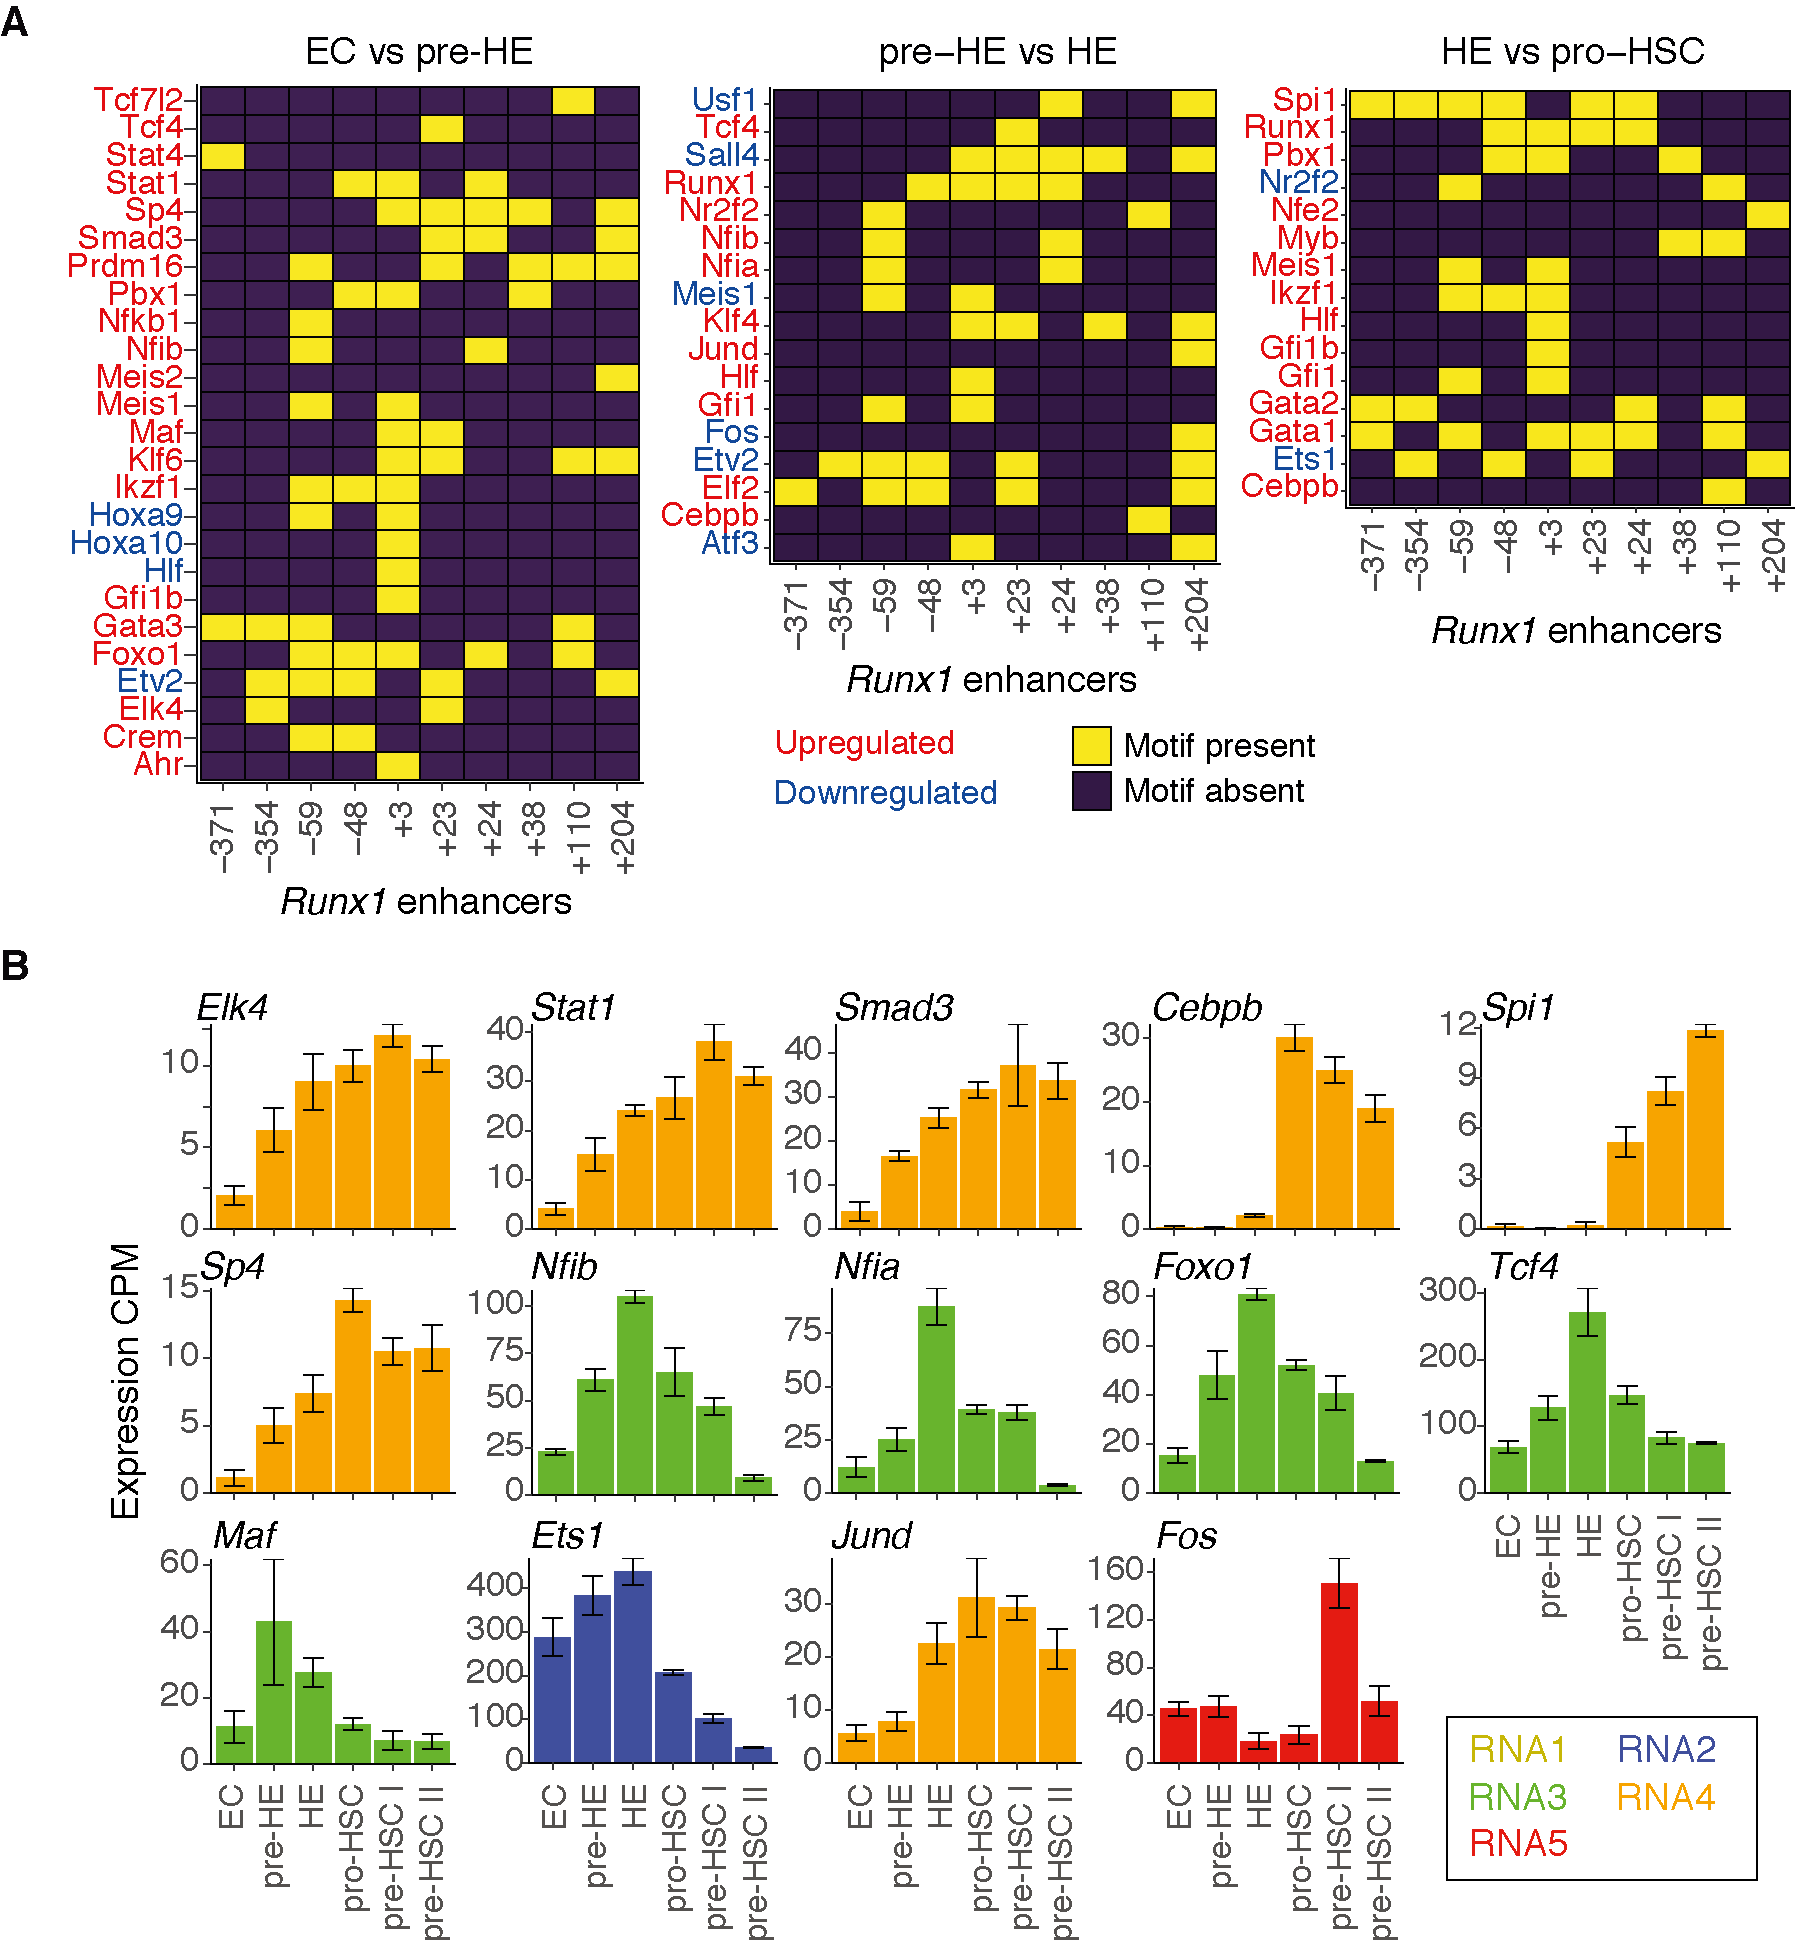
\includegraphics[width=\textwidth,height=\textheight,keepaspectratio]{figures/chapter3/ch3_runx1-motifs.png}
    \caption[{Predicted upstream regulation of \textit{RUNX1}.}]
    {\textbf{Predicted upstream regulation of \textit{RUNX1}.} 
    \textbf{(A)} Heatmap of TF binding motif presence ($\geq$ 1 motifs) at \textit{Runx1} enhancers. Motifs match TFs differentially expressed over the relevant pairwise comparisons, as indicated. Row labels refer to TFs associated with a detected motif, and coloured according to up- or downregulation over the transition. Columns refer to the individual \textit{Runx1} enhancers.
    \textbf{(B)} Gene expression (CPM) for predicted \textit{Runx1} enhancer regulators. Error bars represent standard error of the mean; \textit{n} = 3; \textit{n} = 4 for pre-HE. 
    }
    \label{fig:ch3_runx1-motifs}
\end{figure}

To characterise the factors that may establish the pre-HE state in E8.5 embryos, I first probed TFs upregulated from EC to pre-HE, with motifs in +23/24 enhancers. These include TFs associated with different motif families, such as ETS (Elk4), FOX (Foxo1), zinc fingers (Klf6, Prdm16 and Sp4), Maf-related bZIP (Maf), NFI (Nfib), SMAD (Smad3), STAT (Stat1) and basic Helic-Loop-Helic (bHLH) E2A (Tcf4) (Fig. \ref{fig:ch3_runx1-motifs}A). Among these differentially expressed TFs, \textit{Maf} expression is most specific to pre-HE (Fig. \ref{fig:ch3_runx1-motifs}B). While several of these TFs are reported targets of Runx1 \citep{wang_intersection_2011, zaidi_integration_2002}, their expression precedes \textit{Runx1} and coincides with 23GFP activity, suggesting an additional upstream regulatory role. Elements open in pre-HE, other than +23/24, include -371, -354, and +204 at low levels of accessibility, as well as -59 and -48 at high levels of accessibility (Fig. \ref{fig:ch3_runx1-regulation}). There are a number of TFs upregulated from EC to pre-HE, with predicted motifs in these enhancers. These include motif families such as GATA (Gata3), STAT (Stat4), Rel homology domain (RHD) NF-$\kappa$B (Nfkb1), three amino acid loop extension (TALE) homeobox MEIS (Meis1, Meis2) and PBX (Pbx1), Ikaros zinc finger (Ikzf1), and Creb-related bZIP (Crem). GATA motifs are found in -371, -354, and -59 elements, coinciding with \textit{Gata3} upregulation. Gata3 has recently been reported as essential in aortic endothelium for EHT progression and promotes \textit{Runx1} activity \citep{zaidan_endothelial-specific_2022}, and therefore may be important for the pre-HE population. 

Initiation of endogenous \textit{Runx1} transcription (pre-HE to HE) and \textit{Runx1} upregulation (HE to pro-HSC) are dynamic stages likely induced by key TFs. NFI motifs (Nfia and Nfib) underlie the -59 and +24 enhancers, and \textit{Nfia} and \textit{Nfib} genes are most expressed in HE (Fig. \ref{fig:ch3_runx1-motifs}A-B). Nfib was confirmed to bind to the +24 enhancer (but not the -59 element) using published ChIP-seq data in mammary cells (Appendix \ref{fig:app_runx1-upstream-chip}, \cite{shin_hierarchy_2016}). CEBP motifs were unique to the +110 enhancer, and the \textit{Cebpb} gene upregulated in both transitions. Cebpb binding to the +110 enhancer was validated using published ChIP-seq in pre-B cells (Appendix \ref{fig:app_runx1-upstream-chip}, \cite{van_oevelen_cebp_2015}). Similarly, we find AP-1 motifs (Fos and JunD) motifs underlying the +204 enhancer, and the \textit{Fos} gene is upregulated in the pre-HE to HE transition. Further, the binding of Fos and JunD to the +204 enhancer was confirmed in macrophages and T-cells using published ChIP-seq data (Appendix \ref{fig:app_runx1-upstream-chip}, \cite{roychoudhuri_bach2_2016, eichenfield_tissue_2016}). These observations suggest Cebpb, Fos and Jund as unique regulators of the +110 and +204 enhancers, respectively. \textit{Cebpb} upregulation occurs from HE to pro-HSC, while \textit{Jund} is upregulated from pre-HE to HE, potentially placing Cebpb and Jund as transition-specific drivers. Additionally, Nfia and Nfib are potential novel regulators of the +24 enhancer. It is important to acknowledge that motif analyses based on PWMs are inherently predictive, and while broadly accurate genome wide, may not correctly identify motifs at individual loci. Nevertheless, these analyses provide an interesting preliminary characterisation of potential novel regulators of \textit{Runx1} enhancers.

%Ets1 motifs are also found in the +3, -48, and -354 enhancers, with ChIP-seq evidence in MEL cells \citep{yue_comparative_2014}. 

\subsection{\label{ch3:runx1-targets}Predicted targets of Runx1}

%While endogenous \textit{Runx1} is not expressed in pre-HE, the 23GFP transgene is, indicating that TF signals promoting HE identity are received. Within the EC to pre-HE differential TF subnetwork there is low-level activation of late haematopoietic genes (RNA4, Fig. \ref{fig:ch3_pairwise}A). Activation of the transient module (RNA3), including multiple Notch pathway TFs, Nfib, and Gata3, occurs in pre-HE, preceding \textit{Runx1} expression. This transient regulation increases in pre-HE to HE, with the addition of TFs such as Sox17, which is known to characterise HE \citep{clarke_expression_2013}, and commitment to the haematopoietic lineage with Runx1, Gfi1 and Cebpb. The HE to pro-HSC subnetwork is dominated by committed haematopoietic TFs, such as Myb, Gfi1b and Ikzf1 (Fig. \ref{fig:ch3_pairwise}A). 

\begin{figure}[!t]
    \centering
    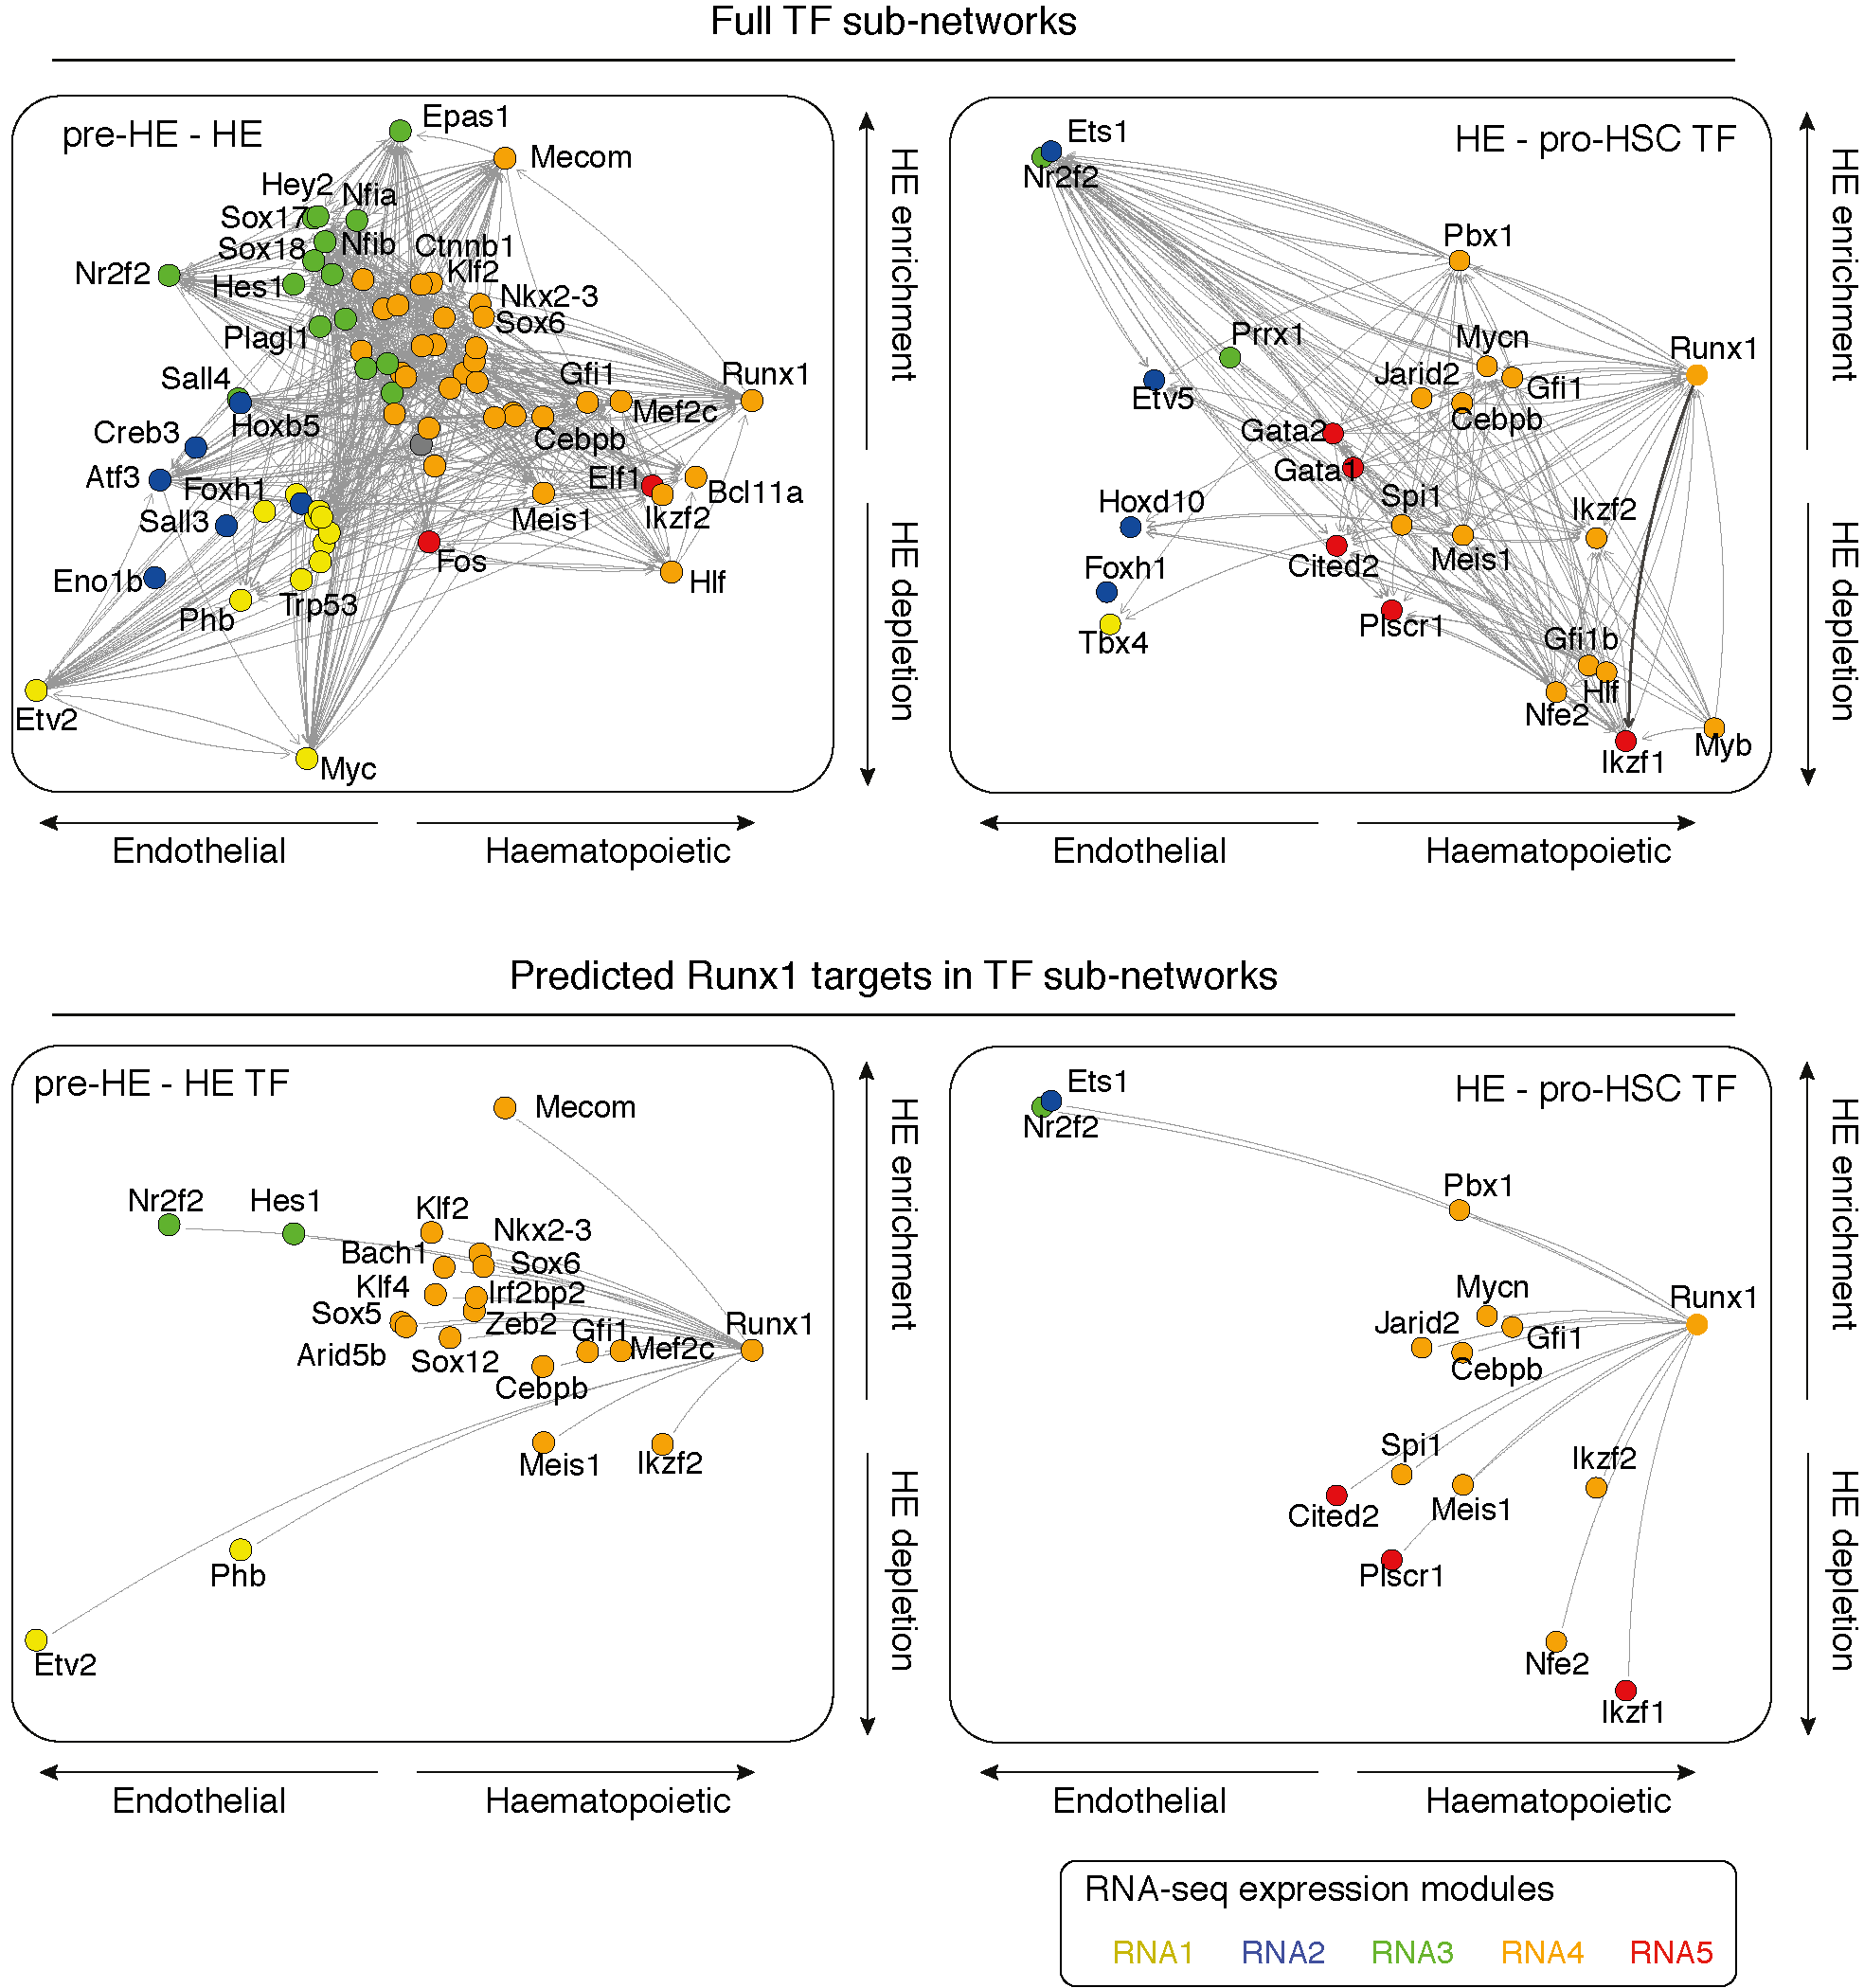
\includegraphics[width=\textwidth,height=\textheight,keepaspectratio]{figures/chapter3/ch3_pairwise.png}
    \caption[{Transition specific TF sub-networks highlight predicted and Runx1 targets.}]
    {\textbf{Transition specific TF sub-networks highlight predicted Runx1 targets.} 
    \textbf{(A)} Sub-networks of EHT GRN (Fig. \ref{fig:ch3_eht-grn}C) illustrating up and downregulated TFs between pre-HE and HE (left) or HE and pro-HSC (right). Nodes are coloured based on expression modules (RNA1-5). Top sub-networks show all differential TFs, and bottom sub-networks show TFs predicted to be regulated by Runx1.
    }
    \label{fig:ch3_pairwise}
\end{figure}

The GRN model predicts Runx1 to regulate many gene targets. An important consideration of these predictions is that RUNX motifs were detected based on a PWM that extends beyond the core consensus motif \citep{kulakovskiy_hocomoco_2018}, and as such likely overestimates predicted Runx1 targets. Despite this caveat, this model offers an exploration of potential Runx1 TF targets. To find key Runx1 targets that may drive EHT, I explored TFs that are differentially expressed between cell type transitions. Direct Runx1 targets are likely to be among those that change in expression just after \textit{Runx1} is upregulated, which is best represented by the pre-HE to HE, and HE to pro-HSC transitions. The GRN model in these transitions detects known Runx1 targets, such as \textit{Spi1} (PU.1) \citep{huang_pu1_2008}, \textit{Gfi1} \citep{wilson_gfi1_2010}, \textit{Nfe2} \citep{wang_aml1_2010} and \textit{Ikzf1} \citep{iacovino_hoxa3_2011} (Fig. \ref{fig:ch3_pairwise}). \textit{Zeb2} is an interesting target that was recently found to be a direct target of Runx1 in a murine kidney cell line, where expression of \textit{Zeb2} in \textit{Runx1} knockout models was sufficient to partially restore the transcriptional phenotype of Runx1 \citep{hass_runx1_2021}. Zeb2 is a known EMT regulator that represses cell-cell junction genes and promotes haematopoietic differentiation \citep{vandewalle_sip1zeb2_2005, li_emt_2017}, and as such may drive the morphological changes that underlie EHT. \textit{Cebpb} is also predicted to be a Runx1 target, and has been previously shown to regulate several key haematopoietic TFs, such as \textit{Gata2} \citep{goode_dynamic_2016}. As shown in Fig. \ref{fig:ch3_runx1-motifs}, Cebpb may regulate the +110 \textit{Runx1} enhancer, resulting in a possible positive feedback loop.

To find key Runx1 targets that may drive EHT, I examined predicted targets that are highly central, as analysed in Fig. \ref{fig:ch3_centrality}A. \textit{Etv2} is a highly central TF in the RNA1 module, with biased expression towards endothelium, that is predicted to be regulated by Runx1 (Fig. \ref{fig:ch3_pairwise}). Interestingly, \textit{Etv2} is expressed in mesoderm and drives both endothelial and haematopoietic programs \citep{liu_induction_2015, menegatti_transcriptional_2019}, and acts as a precursor of HE and EC fate. \textit{Runx1} expression defines the haematopoietic fate of Etv2+ endothelial progenitors \citep{eliades_hemogenic_2016}, and from this analysis may directly repress \textit{Etv2}, in line with the known role of Runx1 to repress the endothelial program \citep{lancrin_gfi1_2012}. Ikzf1 is a prominent central TF in the RNA5 module (late haematopoietic expression) (Fig. \ref{fig:ch3_centrality}A), and is a GRN predicted, and known target of \textit{Runx1} (Fig. \ref{fig:ch3_pairwise}), as has been previously reported in mESC derived EBs \citep{iacovino_hoxa3_2011}. Ikzf1 is expressed in multiple haematopoietic lineages, and is critical for B cell development \citep{nichogiannopoulou_defects_1999,georgopoulos_making_2017,marke_many_2018}. 

This analysis has predicted several known, and novel targets of Runx1. The role of several of these targets, such as Ikzf1, Zeb2, and Cebpb, is not fully understood. It remains a question as to whether Runx1 regulation is important for their normal function and contribution to EHT.

\section{\label{ch3:co-interaction}Runx1 cooperates with TFs to drive EHT processes}

The analysis of the EHT GRN thus far has identified regulatory modules underlying key transitions (section \ref{ch3:profiling}, Fig. \ref{fig:ch3_clusters}), the candidate drivers of each module (section \ref{ch3:centrality}, Fig. \ref{fig:ch3_centrality}), as well as the regulatory context of Runx1 (section \ref{ch3:runx1-context}, Fig. \ref{fig:ch3_runx1-regulation}, Fig. \ref{fig:ch3_runx1-motifs}, and Fig. \ref{fig:ch3_pairwise}). An important consideration in gene regulation is that TFs often do not act independently. While some TFs may act as pioneer factors in specific contexts \citep{zaret_pioneer_2016, zaret_pioneer_2020} and so can function independent of other factors, it is also common for TFs to act in complex with other proteins. The bZIP class of TFs is a classic example of dimerising proteins that modulate TF behaviour \citep{rodriguez-martinez_combinatorial_2017, miller_importance_2009}. Runx1 is also known to cooperate with multiple other TFs \citep{wang_intersection_2011, zaidi_integration_2002, hu_runx1_2011, kim_mutual_1999, goetz_auto-inhibition_2000}, and the expression of \textit{Runx1} leads to genome-wide modulation of Fli1 DNA binding affinities \citep{lichtinger_runx1_2012}. TF cooperation is challenging to explore on a genome-wide scope, but a study of how TFs may cooperate in EHT may offer greater insight into the regulation of EHT. 

\begin{figure}[!t]
    \centering
    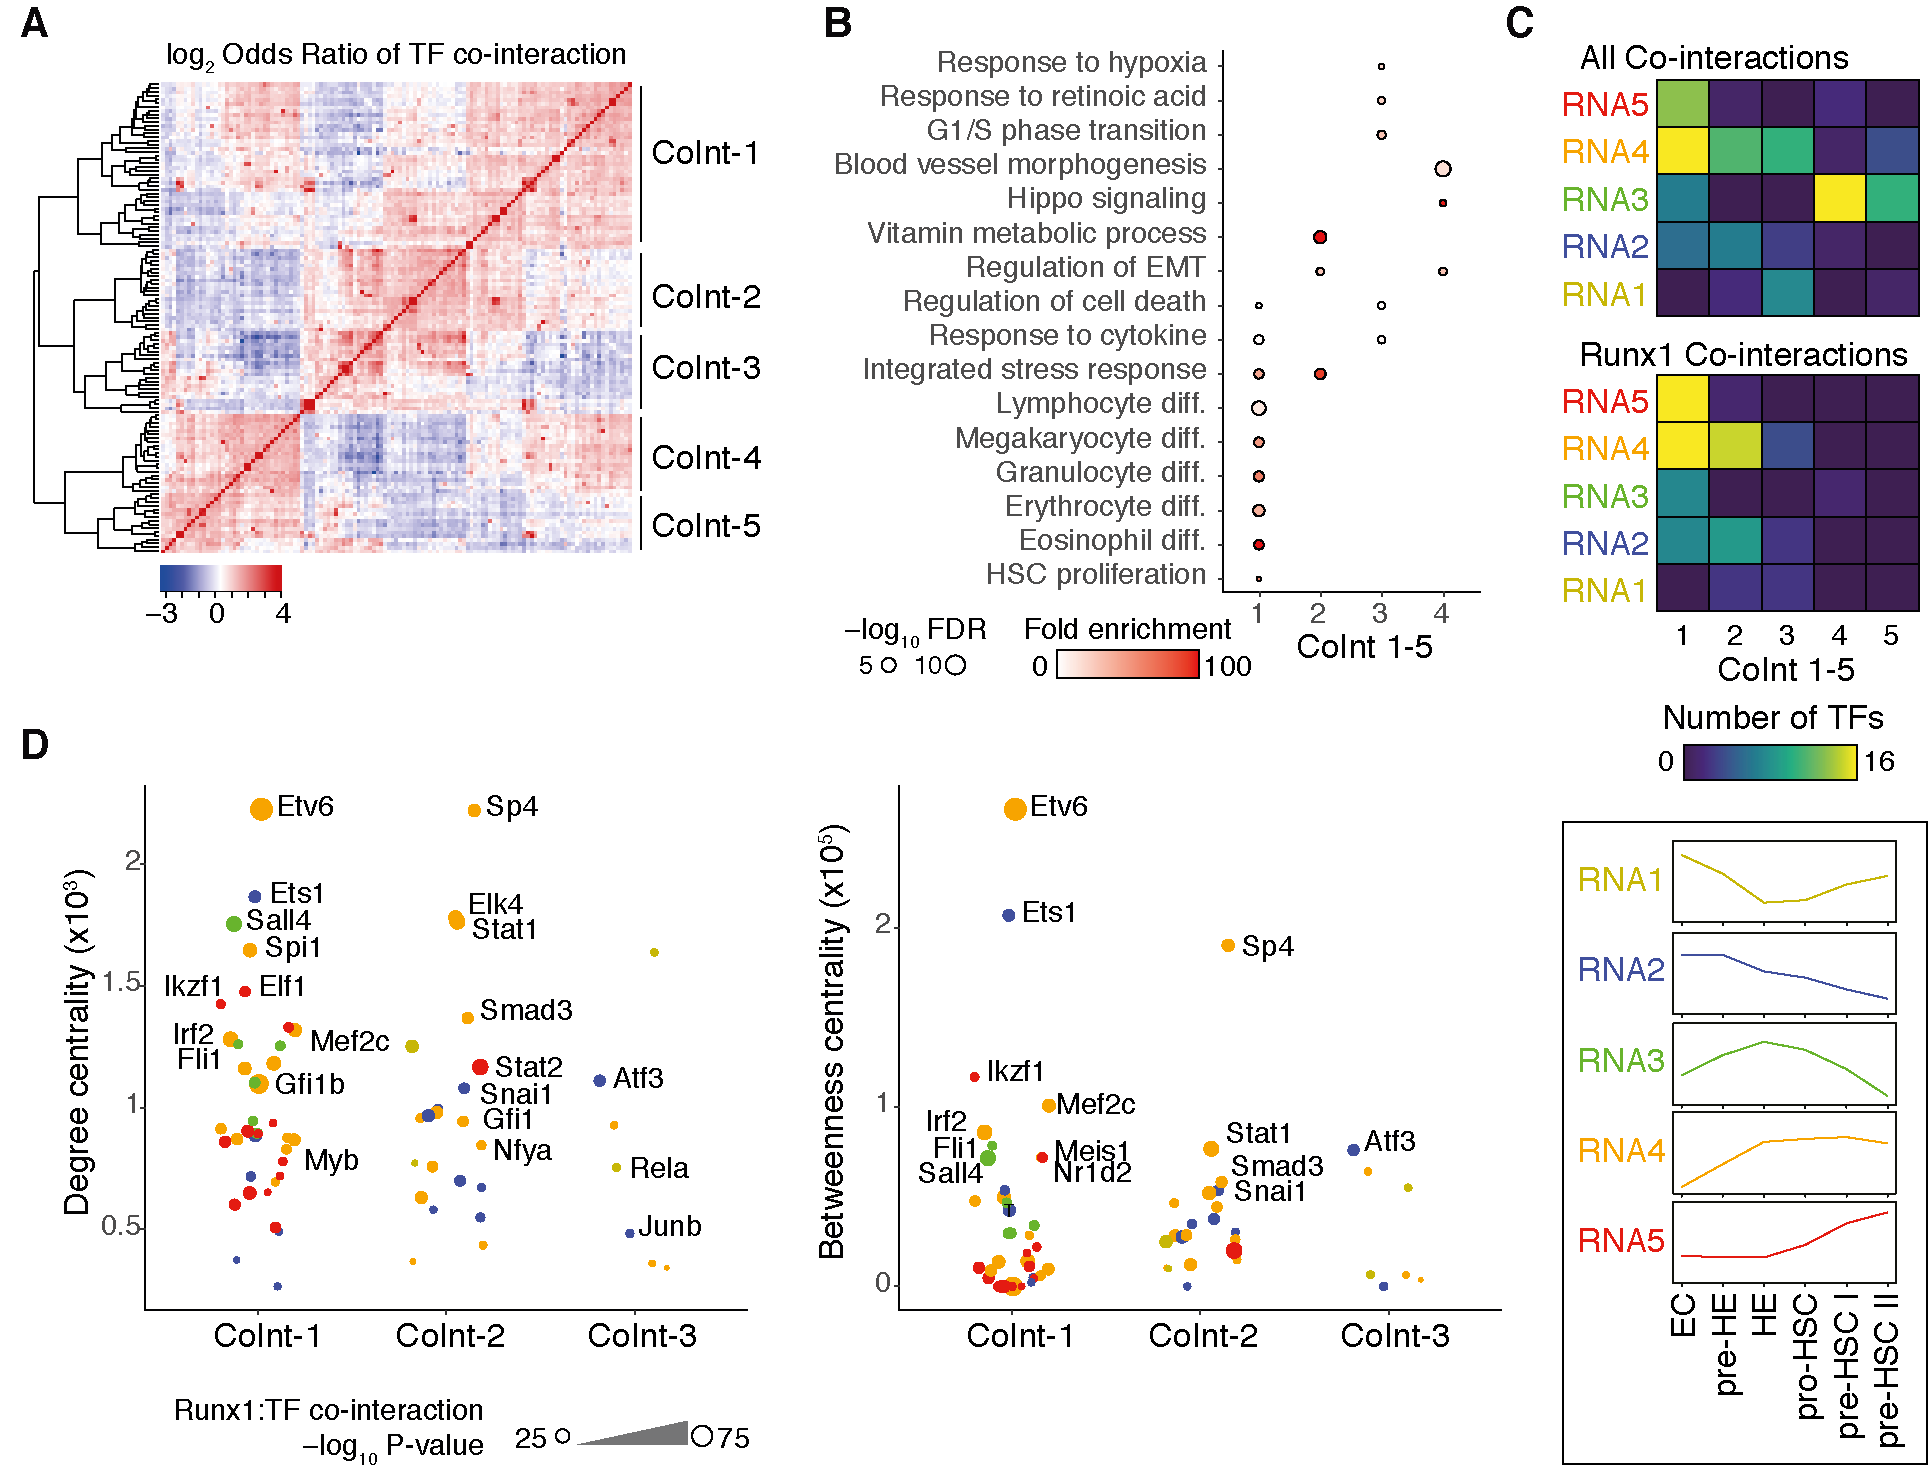
\includegraphics[width=\textwidth,height=\textheight,keepaspectratio]{figures/chapter3/ch3_TF-cointeraction.png}
    \caption[{TFs cooperate in clusters to drive different EHT processes.}]
    {\textbf{TFs cooperate in clusters to drive different EHT processes.} 
    \textbf{(A)} Hierarchical clustered heatmap of odds ratios resulting from Fishers Exact tests comparing the overlap of TF-targets (enhancers) between pairs of TFs. Benjamini and Hochberg correction of P values was performed, and TFs not significant for any interaction were excluded. Clusters describe sets of TFs that commonly act at the same loci, suggesting cooperative regulation. 
    \textbf{(B)} GO biological process enrichment for clusters CoInt 1-4, as in A. Only significant data points shown (P $\leq$ 0.05). Note that no terms were significantly enriched for CoInt-5 .
    \textbf{(C)} Frequency of TFs in each CoInt cluster, as in A, stratified by RNA expression modules (RNA1-5). 
    \textbf{(D)} Stratification of degree (left) and betweenness centrality (right) of the EHT GRN, stratified by CoInt clusters. Only TFs found to significantly co-interact with Runx1 are shown (FDR < 0.05). 
    }
    \label{fig:ch3_TF-cointeraction}
\end{figure}

Here I aimed to apply the GRN model to predict potential cases of TF cooperativity. To predict TF co-interaction in the EHT GRN, I designed an approach to find TF pairs that are predicted to commonly regulate the same enhancer or promoter element. Note that in this thesis I am using "cooperativity" to refer to TFs that function synergistically, and "co-interaction" to refer to TFs predicted to regulate the same sites, as without additional experiments, synergy cannot be proven using the GRN model alone. I performed Fisher's exact tests for all possible TF pairs, in which a positive odds ratio describes TFs that co-interact more frequently than if interactions were random. Odds ratio scores were then grouped into five co-interaction clusters (CoInt 1-5, Fig. \ref{fig:ch3_TF-cointeraction}A). These clusters represent TFs that are predicted to co-interact at the same loci, and by GO analyses each cluster is enriched for different processes (Fig. \ref{fig:ch3_TF-cointeraction}B). Runx1 is in CoInt-1, which is enriched for multiple haematopoietic lineage differentiation processes, in line with driving a haematopoietic program (Fig. \ref{fig:ch3_TF-cointeraction}B). CoInt-2 is related to the stress response, and CoInt-3 involves cell cycle genes and responses to external factors. Interestingly, CoInt-4 is associated with blood vessel morphogenesis and EMT, suggesting a role in modulating aortic endothelium and driving morphological changes.

TFs in CoInt1-3 are enriched in the GRN module RNA4, so are activated in HE or pro-HSCs (Fig. \ref{fig:ch3_TF-cointeraction}C). CoInt-4/5 TFs are instead enriched in the transient expression module (RNA3), and likely represent a cooperative program that drives the effects of the transient module. This is emphasised by CoInt-4 driving EMT processes, in line with RNA3 association with EMT and actin cytoskeletal organisation. Interestingly, when exploring \textit{Runx1} expression correlation with predicted Runx1 targets across GRN modules, \textit{Runx1} is found positively correlated with RNA4-5, but is anti-correlated with RNA-3 (Appendix \ref{fig:app_runx1-cor}). This suggests that Runx1 activity represses transiently expressed genes. Runx1 co-interactors are primarily found in CoInt-1 and CoInt-2 (RNA4 enriched), but not CoInt-4 or CoInt-5 (RNA3 enriched) (Fig. \ref{fig:ch3_TF-cointeraction}C), suggesting that while Runx1 may regulate the transient program (RNA3), it does not cooperate with transient TFs. Runx1 co-interacts with multiple highly central TFs (Fig. \ref{fig:ch3_TF-cointeraction}D), including factors known to cooperate with Runx1 such as Fli1 \citep{lichtinger_runx1_2012}, PU.1 \citep{hu_runx1_2011}, and Ets1 \citep{kim_mutual_1999, goetz_auto-inhibition_2000}. Several TFs that co-interact with Runx1 also display high betweenness centrality, such as Etv6, Ets1, Ikzf1, and Sp4 (Fig. \ref{fig:ch3_TF-cointeraction}D, Fig. \ref{fig:ch1_stress-example}, p.\pageref{fig:ch1_stress-example}). Several of these are predicted targets of Runx1, including Ets1 and Ikzf1. These high betweenness centrality nodes may be critical for GRN pathways, and may cooperate with Runx1. 

\begin{figure}[!t]
    \centering
    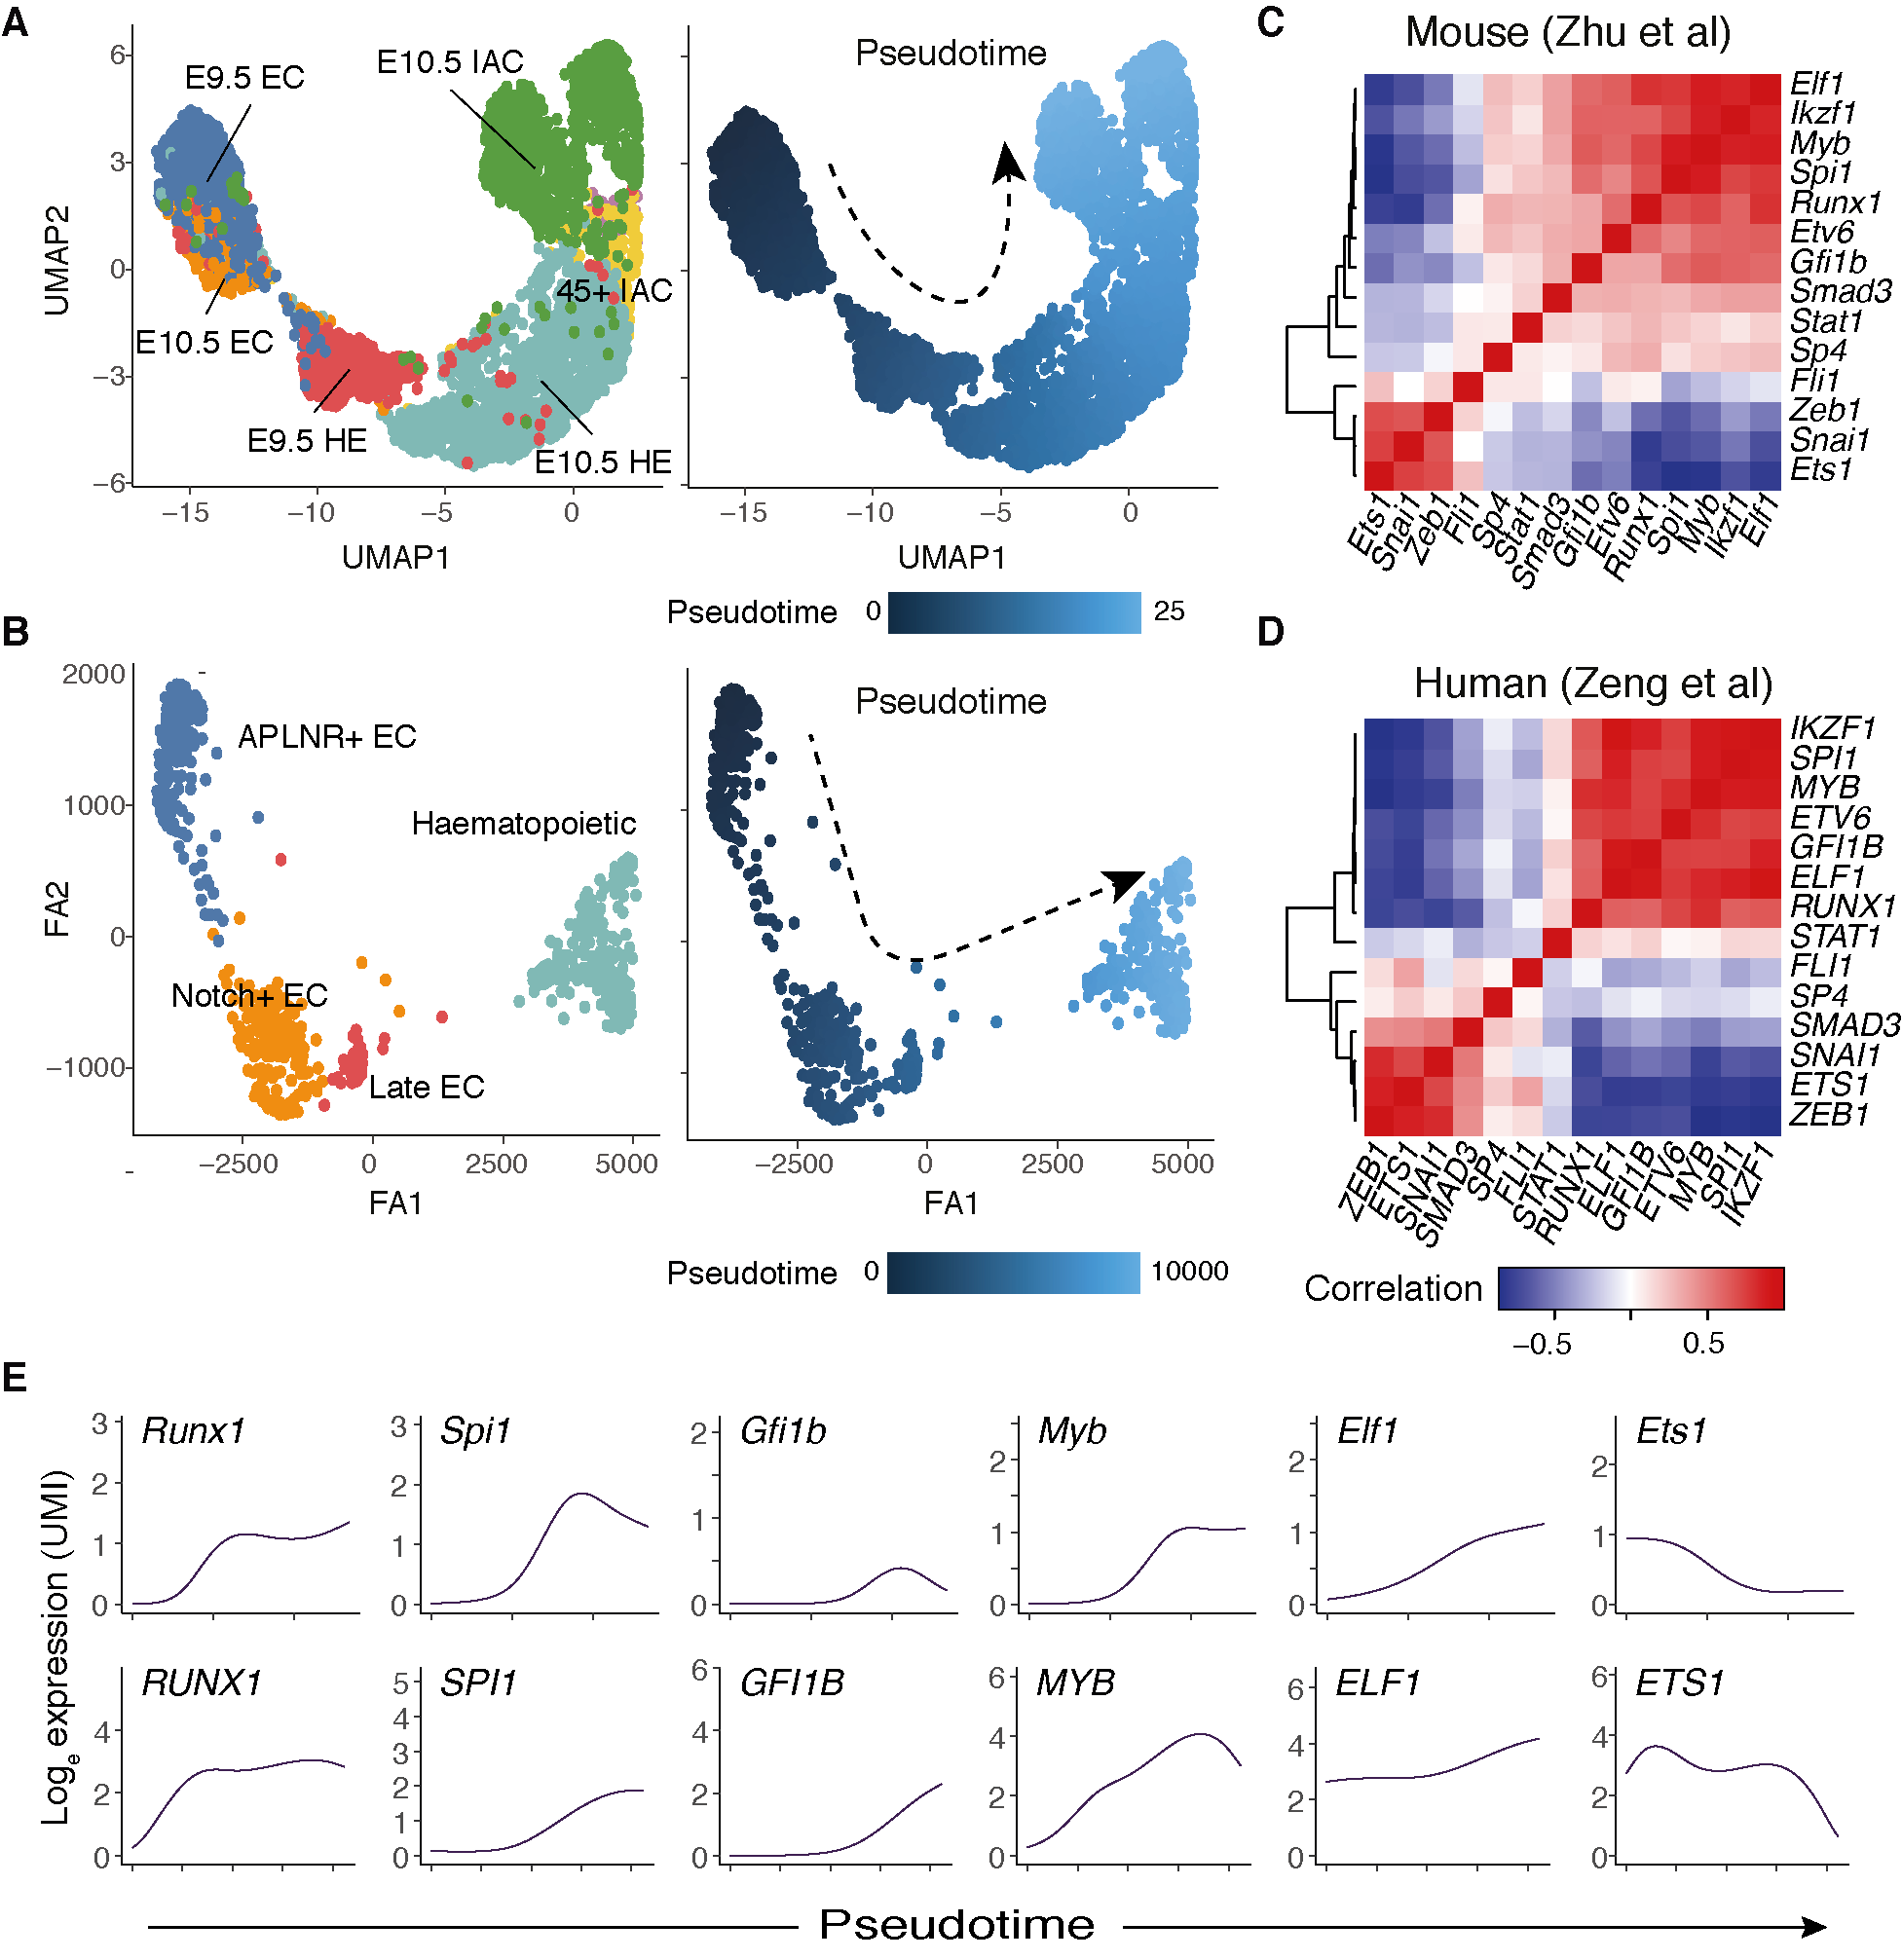
\includegraphics[width=\textwidth,height=\textheight,keepaspectratio]{figures/chapter3/ch3_sc-rna.png}
    \caption[{Gene expression correlation between CoInt-1 TFs in scRNA-seq data.}]
    {\textbf{Gene expression correlation between CoInt-1 TFs in scRNA-seq data.} 
    \textbf{(A, B)} UMAP analysis of mouse EHT scRNA-seq from \cite{zhu_developmental_2020} (A), and Force directed graph (ForceAtlas2, FA2) of human EHT scRNA-seq from \cite{zeng_tracing_2019} (B). Sort populations labelled on left plots. Right plots show Slingshot pseudotime scores. Arrows represent direction of cell differentiation.
    \textbf{(C, D)} Correlation heatmaps of scRNA-seq expression from \cite{zhu_developmental_2020} (C) and \cite{zeng_tracing_2019} (D). See methods section \ref{ch2:pseudo}, p.\pageref{ch2:pseudo} for single cell correlation calculation. 
    \textbf{(E)} scRNA-seq expression of key Runx1 co-interacting TFs for mouse (top) and human (bottom) over pseudotime. Lines indicate smooth fitted values calculated by TradeSeq analysis. 
    \textit{Raw scRNA-seq data from \cite{zhu_developmental_2020} and \cite{zeng_tracing_2019}, reanalysed by me.} 
    }
    \label{fig:ch3_sc-rna}
\end{figure}

This analysis successfully identifies TFs that commonly co-interact co-interact at the same loci, and specifically explores TFs that co-interact with Runx1. However, it does not provide evidence for synergistic cooperativity. Further, the GRN model is based on defined populations from bulk RNA-seq and ATAC-seq, and the relationship between these TFs may differ on a single cell level. To address this, I reanalysed published scRNA-seq EHT datasets in human and mouse \citep{zeng_tracing_2019, zhu_developmental_2020}. To compare gene expression patterns to \textit{Runx1} transcription, I performed pseudotime analysis and correlated gene expression using expression values smoothed along the pseudotime axis (Fig. \ref{fig:ch3_sc-rna}A-B, methods section \ref{ch2:pseudo}, p.\pageref{ch2:pseudo}). This revealed CoInt-1 TFs can be either correlated or anti-correlated with \textit{Runx1} expression (Fig. \ref{fig:ch3_sc-rna}C-E). \textit{Ets1}, \textit{Zeb1} and \textit{Snai1} were consistently anti-correlated with \textit{Runx1}, which may suggest that these factors cooperate with Runx1 in a very specific window before downregulation. Other TFs were positively correlated with \textit{Runx1} expression, with \textit{Etv6}, \textit{Spi1}, \textit{Myb}, \textit{Elf1}, and \textit{Ikzf1} showing the highest correlation. This positive correlation suggests these factors may synergistically cooperate, though further study is required. Overall, this analysis predicts significant TF co-interaction throughout EHT, and this cooperative logic may drive specific EHT processes.

\section{Potential Runx1 driven FFLs in EHT}

This framework to interrogate predicted TF cooperation allowed us to begin exploring how combinatorial regulatory logic may drive different regulatory processes. A common circuit in which TF cooperation occurs is through a FFL, where one TF regulates another TF, and both TFs cooperate to drive regulation of a downstream gene (section \ref{ch1:grn-motifs}, p.\pageref{ch1:grn-motifs}). FFLs are also highly enriched in biological networks \citep{milo_network_2002, mangan_structure_2003}, and are thought to mediate particular gene expression dynamics such as enacting sign-senstive delay in response to signals \citep{mangan_coherent_2003, kalir_coherent_2005}, and acting as pulse generators \citep{mangan_structure_2003, basu_spatiotemporal_2004}. 

\begin{figure}[!t]
    \centering
    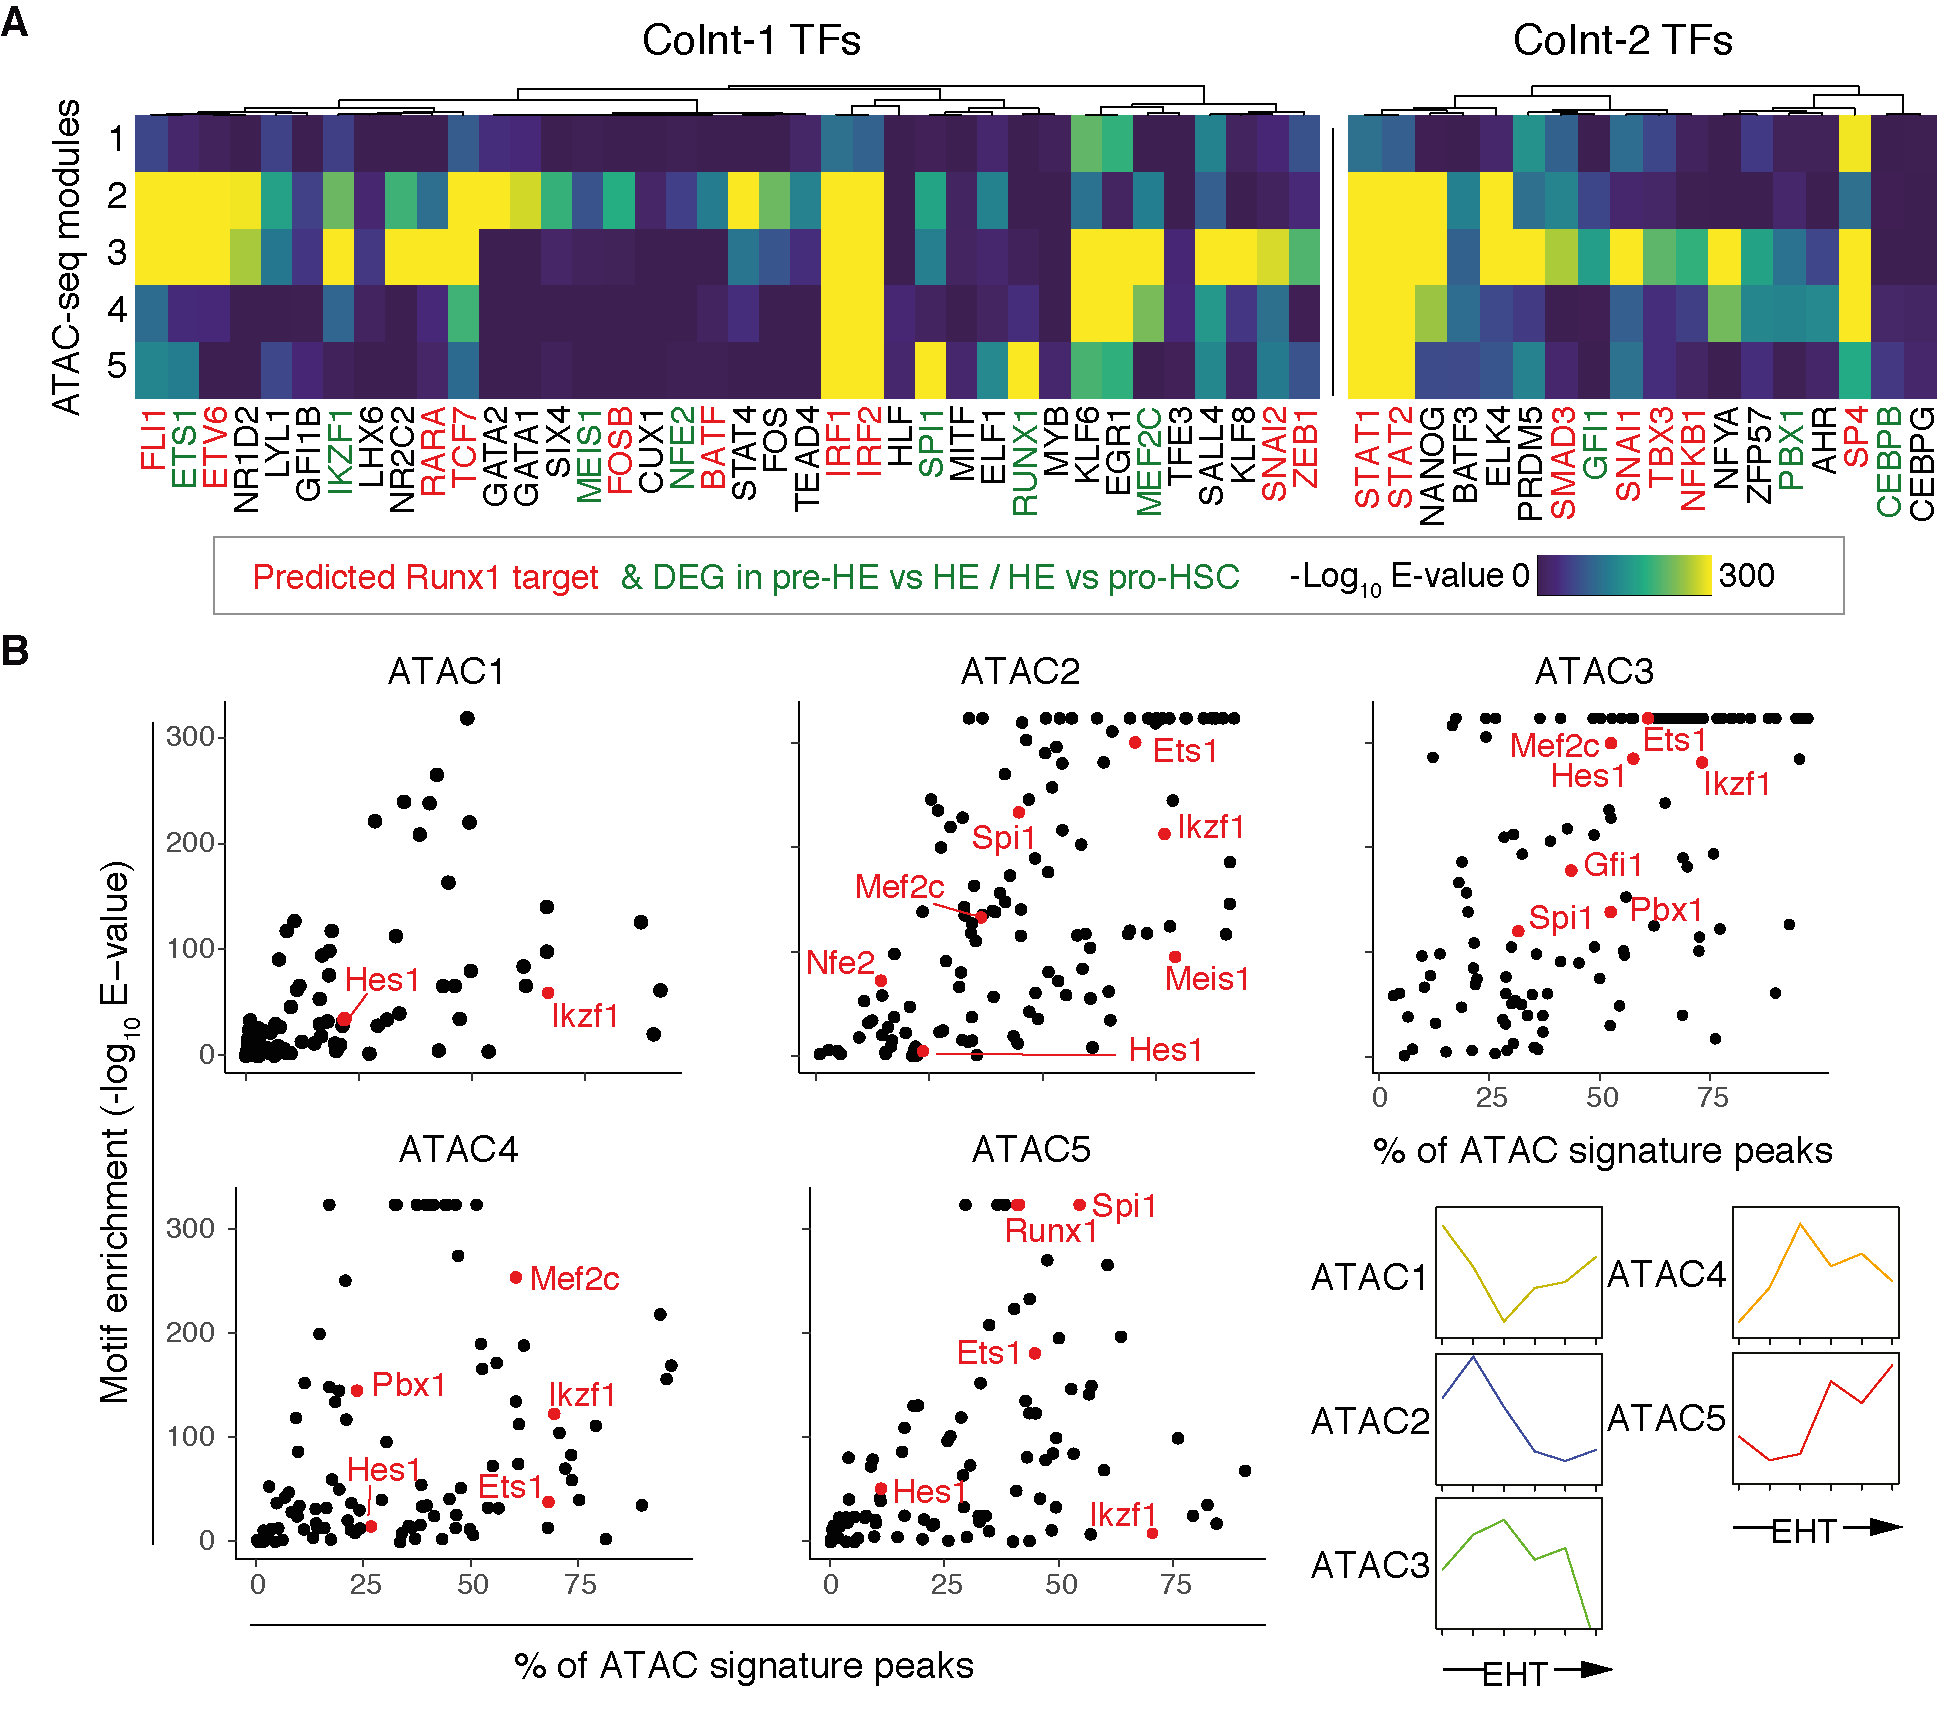
\includegraphics[width=\textwidth,height=\textheight,keepaspectratio]{figures/chapter3/ch3_runx1-TF-motifs.png}
    \caption[{Motif enrichment of Runx1 co-interacting TFs across ATAC-seq accessibility modules.}]
    {\textbf{Motif enrichment of Runx1 co-interacting TFs across ATAC-seq accessibility modules.} 
    \textbf{(A)} Heatmap of TF DNA binding motif enrichment scores (-log\textsubscript{10} E-value) (MEME-AME, methods section \ref{ch2:motifs}, p.\pageref{ch2:motifs}) within ATAC-seq elements found in modules ATAC1-5. Rows indicate peak sets from ATAC1-5 modules, columns indicate motif enrichment. Column labels refer to TFs (as in CoInt-1 and CoInt-2 co-interactions clusters) for which a motif PWM is associated, and used for enrichment analysis. TFs in CoInt-1 and CoInt-2 that co-interact with Runx1 shown. TF labels are coloured red if they are GRN predicted targets of Runx1, or green if they are predicted targets of Runx1 and are differentially expressed in either the pre-HE to HE, or HE to pro-HSC transitions (see Fig. \ref{fig:ch3_pairwise}). 
    \textbf{(B)} Relationship between motif enrichment scores at ATAC-seq modules (ATAC1-5), and proportion of elements in each module containing motif. Note the motif for Hes1 was sourced from the full HOCOMOCO TF motif database (see section \ref{ch2:motifs}, p.\pageref{ch2:motifs} for database details). Nodes highlighted in red include the Hes1 motif, and TF motifs associated with predicted Runx1 targets, differentially expressed the pre-HE to HE or HE to pro-HSC transitions.
    }
    \label{fig:ch3_runx1-TF-motifs}
\end{figure}

Several TFs within CoInt-1 and CoInt-2 were found to frequently co-interact with Runx1, such as the high betweenness centrality TFs Etv6, Ets1, Sp4, and Ikzf1 (Fig. \ref{fig:ch3_TF-cointeraction}C-D). Additionally, a number of these co-interacting TFs were also found to be targets of Runx1, and in particular were differentially expressed subsequent to the onset of \textit{Runx1} expression. These include Ets1, Ikzf1, Meis1, Nfe2, PU.1, Mef2c, Gfi1, Pbx1, and Cebpb (Fig. \ref{fig:ch3_runx1-TF-motifs}A, Fig. \ref{fig:ch3_pairwise}, Fig. \ref{fig:ch3_TF-cointeraction}), suggesting that Runx1 has the capacity to form cooperative FFLs with these TFs. I next probed what processes these co-interacting TFs may regulate. While the majority of CoInt-1 and CoInt-2 TFs are expressed in RNA4 and RNA5 modules (Fig. \ref{fig:ch3_TF-cointeraction}C), they may not necessarily interact with ATAC4 and ATAC5 accessible elements. To determine what ATAC-seq modules CoInt-1 and CoInt-2 TFs are most likely to regulate, I performed TF binding motif enrichment analysis across ATAC1-5 elements (Fig. \ref{fig:ch3_runx1-TF-motifs}A). For example, RUNX motifs are highly enriched in ATAC5 over other modules, suggesting Runx1 binds to and regulates pre-HSC-active genes. This analysis does not preclude Runx1 from regulating targets in other modules, and in-fact many of the TFs predicted to co-interact with Runx1 are instead associated with endothelial and transient accessible sites (ATAC2 and ATAC3). Runx1 may therefore cooperate with TFs across different ATAC-seq accessibility modules, in possible FFL configurations. 

ETS motif TFs (Ets1, PU.1) are enriched in ATAC-seq modules ATAC2, ATAC3 and ATAC5, with some specificity differentiating PU.1 and Ets1 HOCOMOCO PWMs resulting in higher enrichment for the PU.1 PWM in ATAC5 (Fig. \ref{fig:ch3_runx1-TF-motifs}A-B). Motifs for Meis1 and Nfe2 are enriched in ATAC2 peaks, suggesting that they interact with the endothelial program (Fig. \ref{fig:ch3_runx1-TF-motifs}A-B). Meis1 has been reported to promote EC development in zebrafish \citep{minehata_meis1_2008}, and \textit{Meis1} knockout studies result in abnormal vasculature \citep{hisa_hematopoietic_2004}. Pbx1 motifs are enriched in both ATAC3 and ATAC4 elements (Fig. \ref{fig:ch3_runx1-TF-motifs}A-B), and Pbx1 is known to mediate HSC quiescence, possibly through activation of Tgf-$\beta$ related genes \citep{ficara_pbx1_2008}, and as such may regulate Tgf-$\beta$ activity in IAC populations. Motifs for Ikzf1, Mef2c and Gfi1 are biased towards ATAC3 (Fig. \ref{fig:ch3_runx1-TF-motifs}A-B), suggesting these factors regulate the transiently accessible module. Mef2c is known for its roles in megakaryopoiesis and B-cell development \citep{gekas_mef2c_2009}, and Ikzf1 is a TF critically required for B-cell development \citep{nichogiannopoulou_defects_1999}, though their role in EHT is unclear.

\begin{figure}[!t]
    \centering
    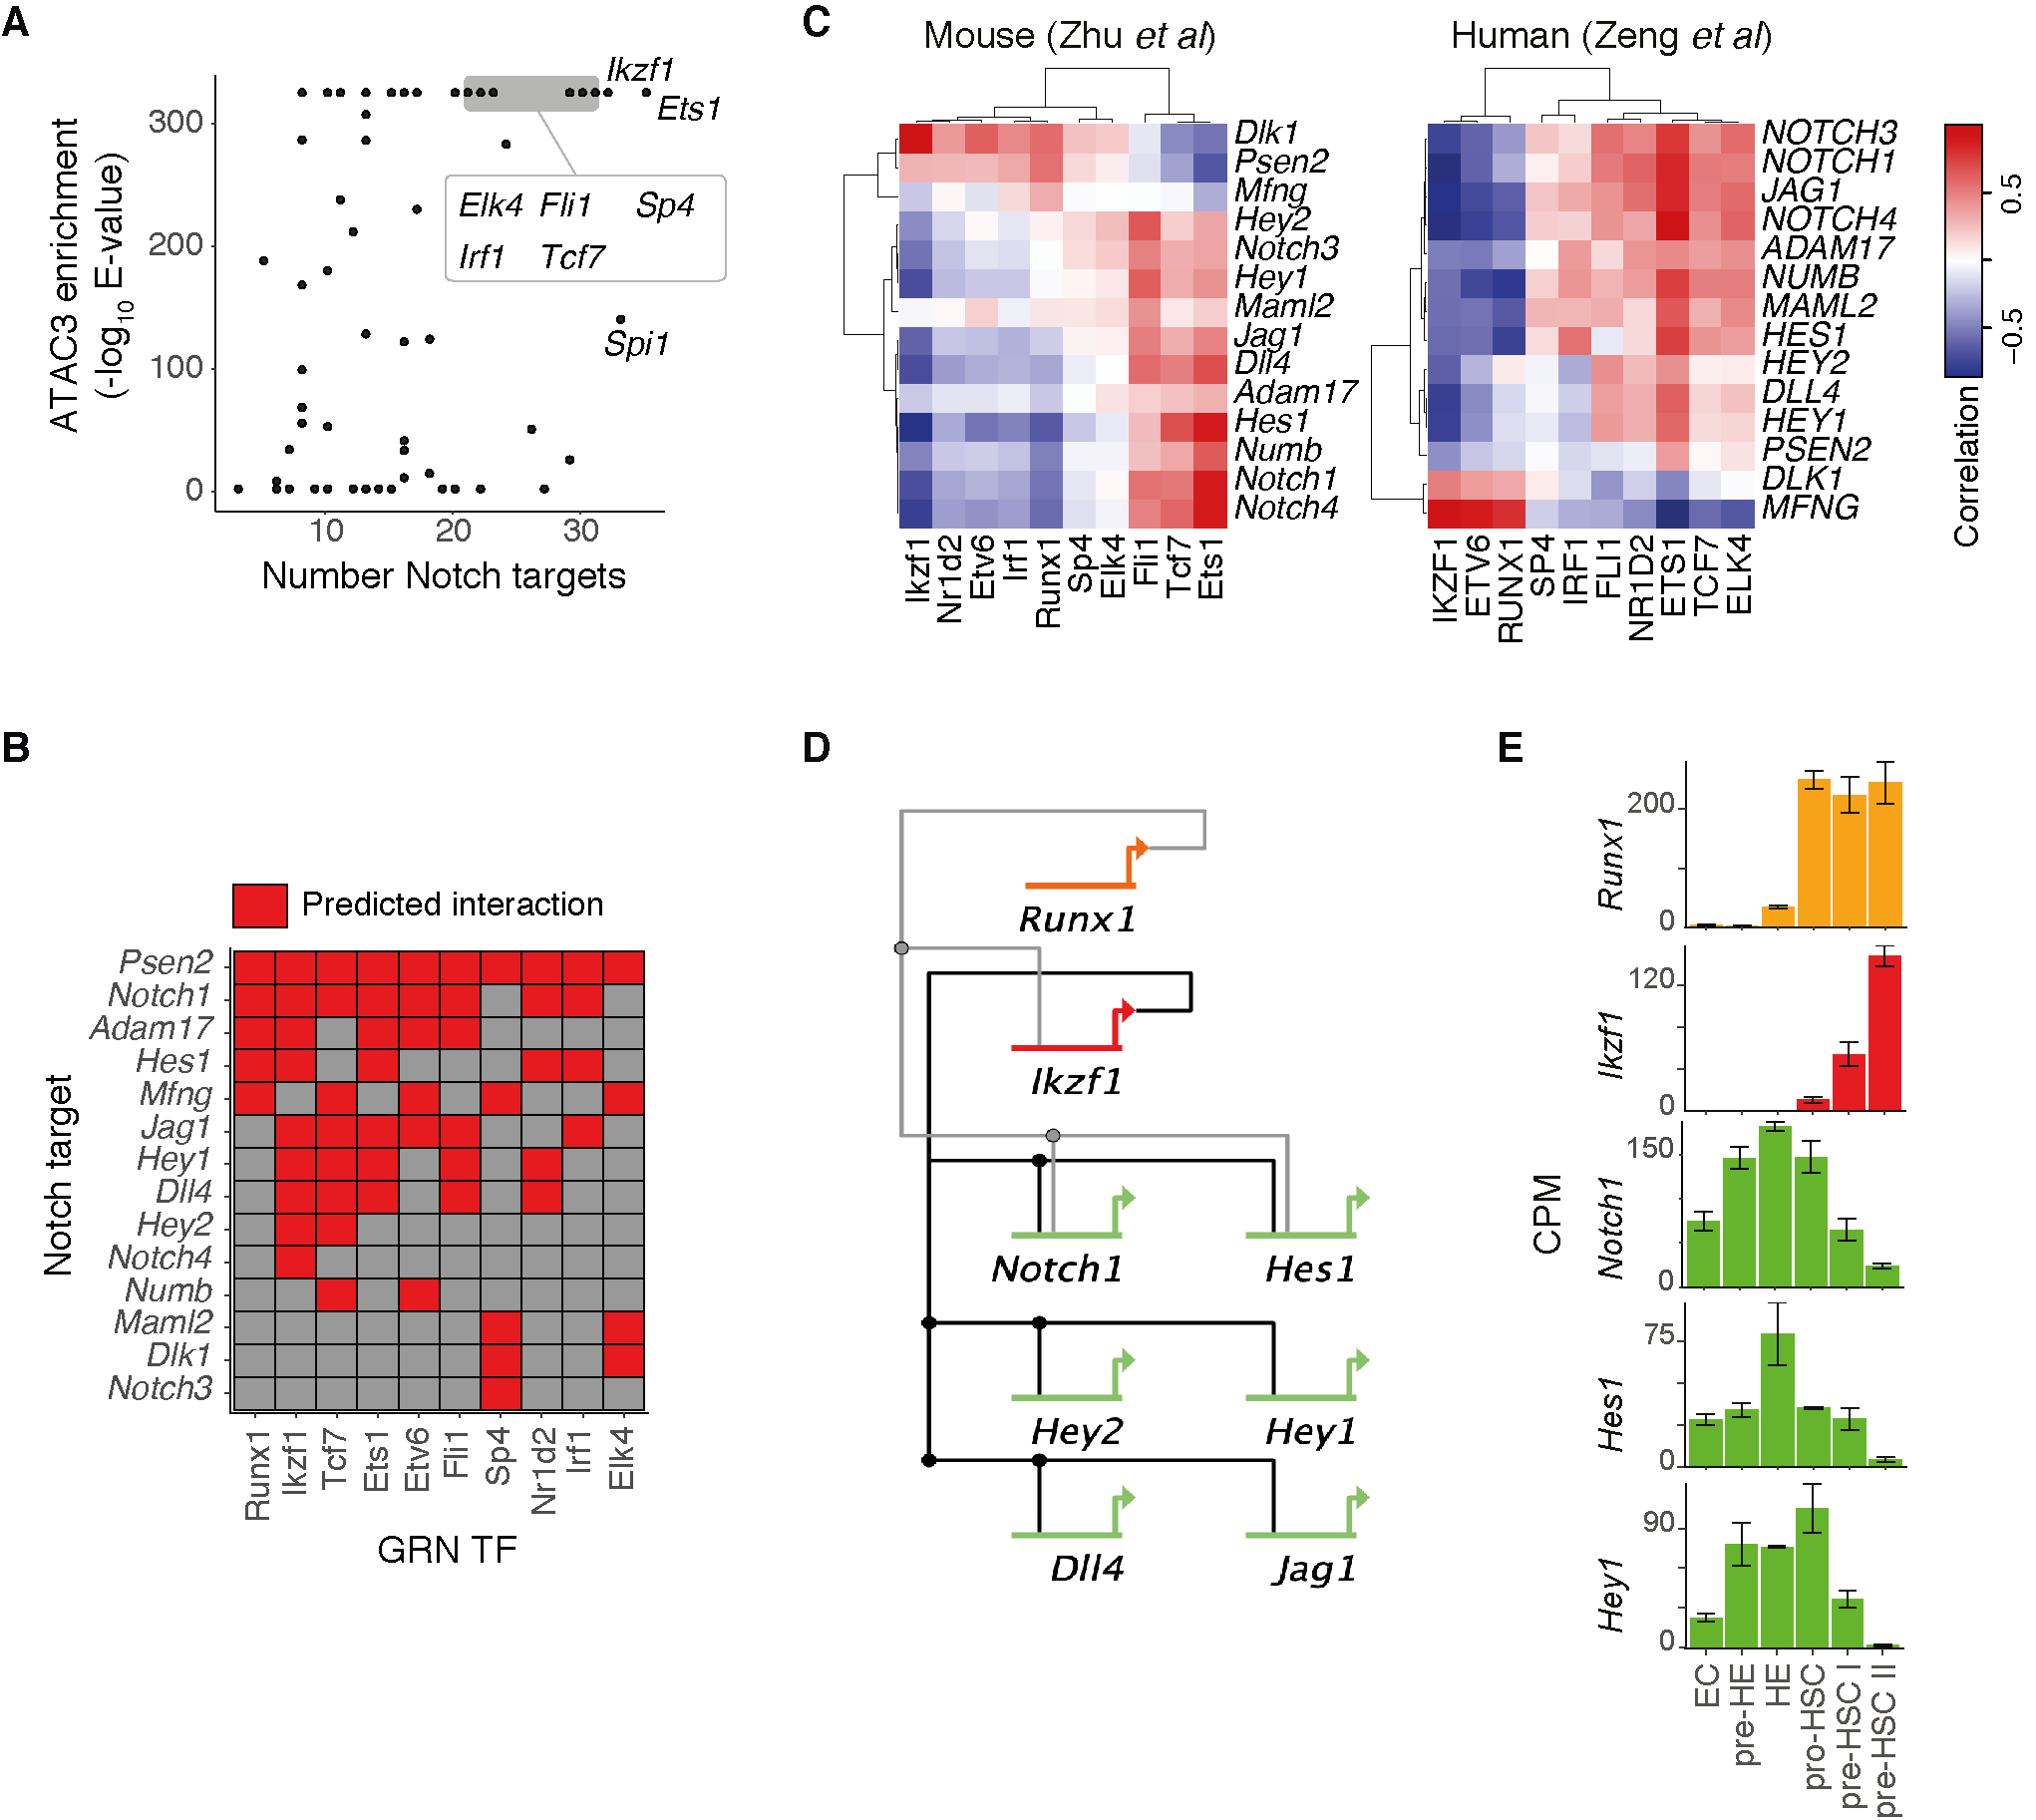
\includegraphics[width=\textwidth,height=\textheight,keepaspectratio]{figures/chapter3/ch3_runx1-ikzf1-notch.png}
    \caption[{Runx1 and Ikzf1 cooperate to repress the Notch pathway through a Runx1:Ikzf1:\textit{Hes1} FFL.}]
    {\textbf{Runx1 and Ikzf1 cooperate to repress the Notch pathway through a Runx1:Ikzf1:\textit{Hes1} FFL.} 
    \textbf{(A)} Relationship between enrichment of TF motifs at ATAC3 elements, and the number of GRN predicted TF targets in the Notch pathway (GO:0007219). 
    \textbf{(B)} TF interaction matrix showing predicted regulation of TFs at Notch pathway targets. TF regulators are shown as columns, and predicted Notch pathway targets as rows. 
    \textbf{(C)} Correlation heatmaps from scRNA-seq EHT data. 
    \textbf{(D)} Circuit illustrating predicted regulation of Notch genes by Runx1 (light grey lines) and Ikzf1 (dark grey lines). 
    \textbf{(E)} Gene expression (CPM) for \textit{Runx1}, \textit{Ikzf1}, and select Notch genes. Error bars represent standard error of the mean; \textit{n} = 3; \textit{n} = 4 for pre-HE. 
    \textit{Raw scRNA-seq data from \cite{zhu_developmental_2020} and \cite{zeng_tracing_2019}, reanalysed by me.} 
    }
    \label{fig:ch3_runx1-ikzf1-notch}
\end{figure}

\subsection{\label{ch3:notch}A Runx1 and Ikzf1 driven FFL regulates Notch pathway genes}

An interesting aspect of Runx1 activity in the EHT GRN model is that Runx1 targets in the RNA3 expression module are anti-correlated with \textit{Runx1} expression (Appendix \ref{fig:app_runx1-cor}), suggesting that Runx1 represses genes in the transient network. I next explored the capacity for Runx1, in cooperation with other TFs, to repress transiently expressed genes. In section \ref{ch3:profiling}, I found the transient expression and accessibility modules (RNA3 and ATAC3) to be enriched for Notch signalling by GO analysis (Fig. \ref{fig:ch3_clusters}C-D). Interestingly, motifs for the Notch target gene, \textit{Hes1}, are also highly enriched at transient elements (ATAC3, Fig. \ref{fig:ch3_runx1-TF-motifs}B). This suggests that Notch signalling is a prominent regulator of the transient EHT network. I screened all TFs enriched in ATAC3 for possible regulation of the Notch pathway, by quantifying the number of GRN predicted targets at Notch signalling related genes (GO:0007219) (Fig. \ref{fig:ch3_runx1-ikzf1-notch}A). The TFs that were found to most frequently target the Notch pathway within the GRN model were Ikzf1, PU.1 and Ets1. Previous study identified Ikzf1 as a repressor of Notch signalling in T-cell development \citep{kleinmann_ikaros_2008}, and this analysis suggests that this activity is present in EHT as well. Ikzf1 is of particular interest, as it is predicted to be regulated by Runx1 (section \ref{ch3:runx1-targets}, Fig. \ref{fig:ch3_pairwise}), is found to co-interact with Runx1 (section \ref{ch3:co-interaction}, Fig. \ref{fig:ch3_TF-cointeraction}), and is a highly central TF within the RNA5 gene expression module (section \ref{ch3:centrality}, Fig. \ref{fig:ch3_centrality}), suggesting it is an active driver of late-EHT populations. IKZF motifs are significantly enriched at all ATAC-seq modules, but most enriched at transiently accessible (ATAC3) sites (Fig. \ref{fig:ch3_runx1-TF-motifs}B). As Ikzf1 can deactivate targets through recruitment of HDAC \citep{marke_many_2018}, and its motif is highly enriched at transiently accessible (ATAC3) sites, this positions it as a potential repressor of the transient EHT network. More specifically, it may repress Notch pathway genes, which is a known behaviour of Ikzf1 in T-cell development \citep{kleinmann_ikaros_2008}, but is an as yet unexplored interaction in EHT. 

As \textit{Ikzf1} is a predicted target of Runx1, and Ikzf1 co-interacts with Runx1, it is possible that these factors cooperate at Notch genes in a FFL circuit. While Ikzf1 is predicted to regulate many Notch genes, Runx1 is predicted to regulate relatively few, such as \textit{Notch1} and \textit{Hes1} (Fig. \ref{fig:ch3_runx1-ikzf1-notch}B). Ikzf1 also regulates these loci, and additionally targets \textit{Hey1}, \textit{Hey2}, \textit{Jag1} and \textit{Dll4}. I used the mouse and human scRNA-seq EHT data from \cite{zhu_developmental_2020} and \cite{zeng_tracing_2019}, respectively, to compare expression profiles (Fig. \ref{fig:ch3_runx1-ikzf1-notch}C). \textit{Runx1} expression was strongly anti-correlated with \textit{Hes1} and \textit{Notch1}, but not \textit{Hey1} or \textit{Hey2} (Fig. \ref{fig:ch3_runx1-ikzf1-notch}C), in line with its predicted regulation. \textit{Ikzf1} was instead anti-correlated with each of its predicted targets. Together, this suggests a key role for Ikzf1 in repressing Notch signalling, and may cooperate with Runx1 at a subset of Notch pathway genes. GRN predicted interactions downstream of Runx1 and Ikzf1 suggest a FFL circuit, where Runx1 activates \textit{Ikzf1}, and both TFs cooperate to repress \textit{Notch1} and \textit{Hes1} (Fig. \ref{fig:ch3_runx1-ikzf1-notch}D). Additionally, a TF cascade is predicted where Ikzf1 regulates several Notch genes independently of Runx1. Based on expression data, Runx1 does not appear to be sufficient to fully repress \textit{Notch1} or \textit{Hes1} alone, and full inactivation of these genes does not occur until \textit{Ikzf1} is upregulated in pre-HSC I and pre-HSC II populations (Fig. \ref{fig:ch3_runx1-ikzf1-notch}E). This is in line with the hypothesis that Runx1 and Ikzf1 can cooperate with each other, and may synergise to maximise repression of the Notch pathway.

\begin{figure}[!b]
    \centering
    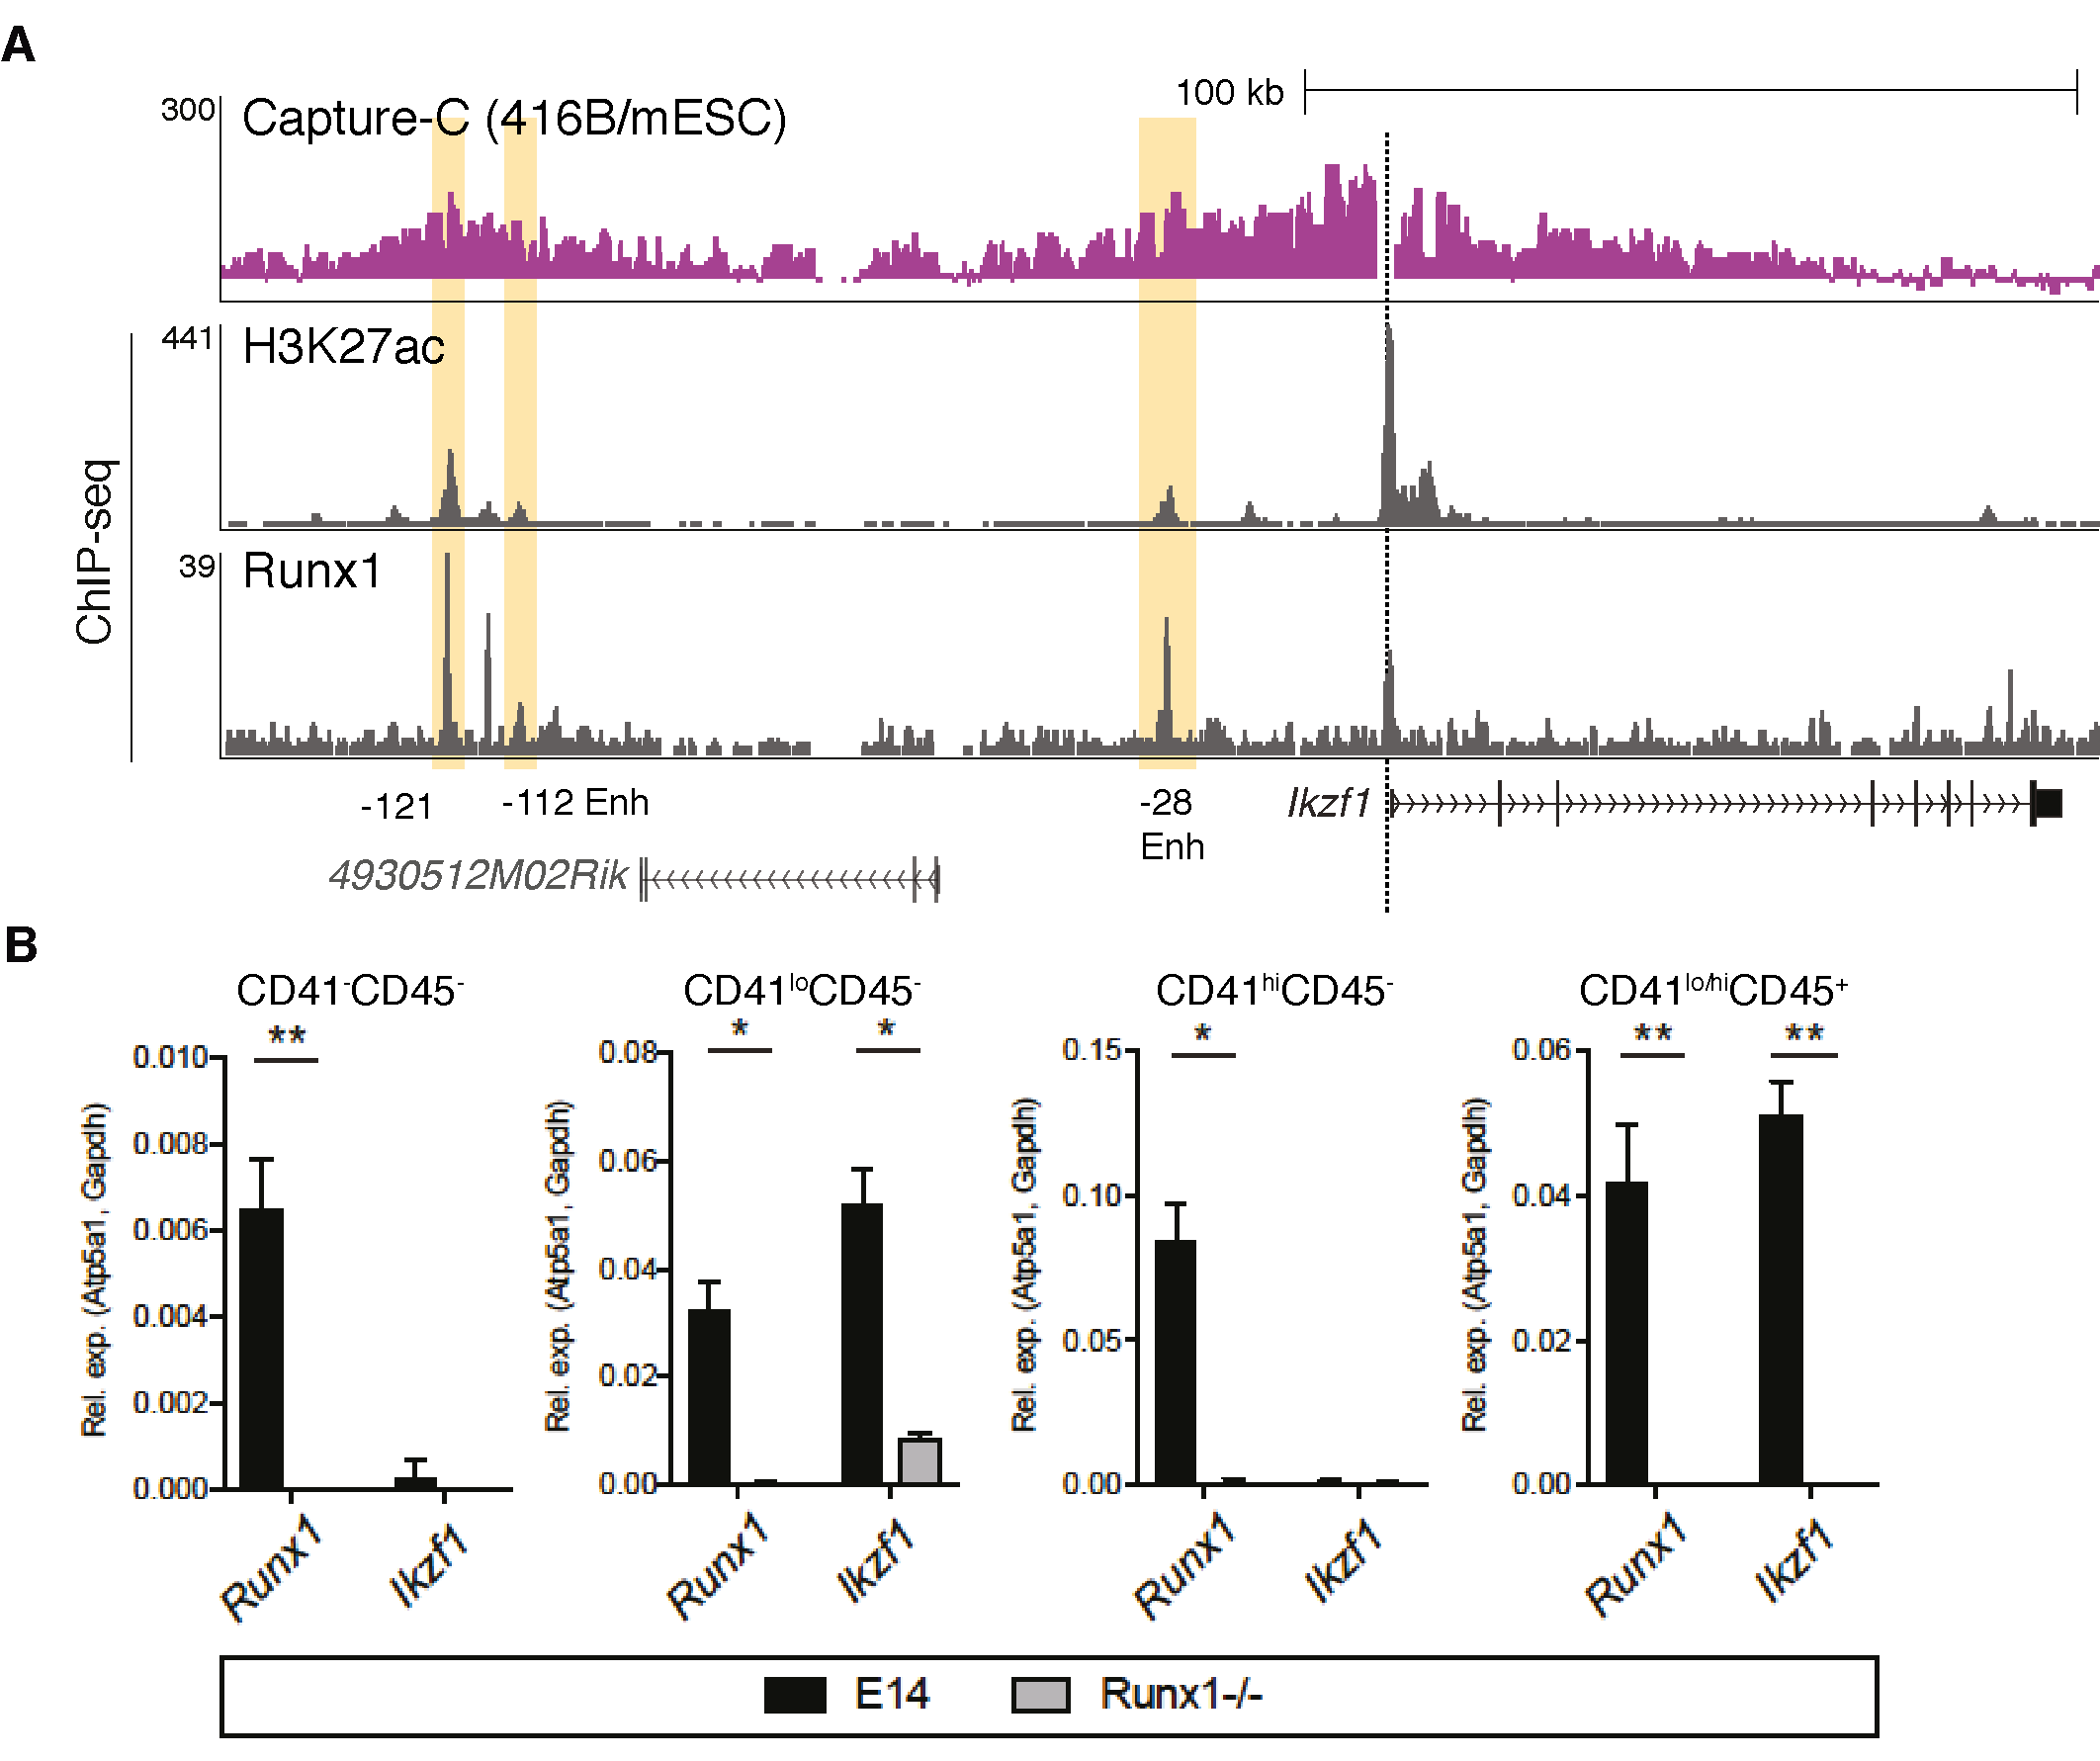
\includegraphics[width=0.9\textwidth,height=\textheight,keepaspectratio]{figures/chapter3/ch3_runx1-ikzf1.png}
    \caption[{Validation of Runx1:\textit{Ikzf1} interaction.}]
    {\textbf{Validation of Runx1:\textit{Ikzf1} interaction.} 
    \textbf{(A)} Capture-C tracks over the \textit{Ikzf1} locus (top), using the \textit{Ikzf1} promoter as the capture point (dashed line). Reads normalised as 416B signal (active \textit{Runx1}) over mESC signal (inactive \textit{Runx1}). Runx1 and H3K27ac ChIP-seq from 416B cells (bottom). GRN enhancer elements annotated. 
    \textbf{(B)} qRT-PCR assaying \textit{Runx1} and \textit{Ikzf1} expression at day 7 of differentiation of \textit{Runx1}\textsuperscript{+/+} and \textit{Runx1}\textsuperscript{-/-} mESC lines (\textit{n} = 3). Expression normalised to \textit{Atp5a1} and \textit{Gapdh}. ns: not significant, * P < 0.05 , ** P < 0.01. 
    \textit{Capture-C (A) performed and analysed by D. Owens, and qRT-PCR (B) performed by L. Greder. ChIP-seq data (A) sourced from \cite{schutte_experimentally_2016} and analysed by me.} 
    }
    \label{fig:ch3_runx1-ikzf1}
\end{figure}

To functionally validate the existence of these FFL circuits (Fig. \ref{fig:ch3_runx1-ikzf1-notch}D), it is first important to explore the Runx1 driven regulation of \textit{Ikzf1}. The EHT GRN predicted Runx1 to regulate the -28, -112, and -121 kb \textit{Ikzf1} enhancers upstream of the promoter. The -121 and -28 elements were characterised in \cite{alomairi_integration_2020}, where the -121 element was found to be a strong enhancer in CD4\upos{}CD8\upos{} T-cells. The enhancer potential, and relevance of these enhancer elements to EHT, is as yet unclear, but may act to drive Runx1 and Ikzf1 FFLs. To validate that these have enhancer features, I reanalysed published Runx1 and H3K27ac ChIP-seq data in 416B cells (CD34+ myeloid cell line) \citep{schutte_experimentally_2016}, and capture-C analysis performed by D. Owens (de Bruijn lab). These data found the -28, -112 and -121 elements were bound by Runx1 and marked by H3K27ac, and to physically interact with the \textit{Ikzf1} promoter (Fig. \ref{fig:ch3_runx1-ikzf1}A). Runx1 was functionally validated to regulate \textit{Ikzf1} by L. Greder (de Bruijn lab), who showed that \textit{Ikzf1} expression was reduced in \runxnull{} cells (Fig. \ref{fig:ch3_runx1-ikzf1}B). Further work from L. Greder (de Bruijn lab, unpublished) has functionally tested the Runx1:Ikzf1:\textit{Hes1} FFL circuit in mESC differentiation cultures (Appendix \ref{fig:app_notch-ffl-validation}). This experiment used \textit{Ikzf1\textsuperscript{-/-}} and \textit{Ikzf1\textsuperscript{+/+}} mESCs, and used a \textit{Runx1-ERt2} fusion to control Runx1 nuclear translocation. Ikzf1 and Runx1 activity is referred to here as active (Ikzf1+/Runx1+) or inactive (Ikzf1-/Runx1-). It was found that in Ikzf1-/Runx1+ conditions, Runx1 appears to promote \textit{Hes1} expression over Ikzf1-/Runx1- conditions (Appendix \ref{fig:app_notch-ffl-validation}), contrary to the GRN-predicted activity of Runx1 at this locus. In Ikzf1+/Runx1- conditions, \textit{Hes1} is instead repressed compared with Ikzf1-/Runx1- conditions, in line with the predicted repressive activity of Ikzf1. Interestingly, \textit{Hes1} is maximally repressed only in Ikzf1+/Runx1+ conditions, suggesting that both Runx1 and Ikzf1 are required for full downregulation of the gene. These analyses build evidence for a functional Runx1:Ikzf1:\textit{Hes1} FFL circuit that drives repression of \textit{Hes1}, and is a potential mechanism to drive Notch pathway suppression in pre-HSC I and pre-HSC II populations where \textit{Ikzf1} is expressed.


\section[Maf and Lef1 cooperation may drive cytoskeletal remodelling and EMT processes]{\label{ch3:maf-lef1}Maf and Lef1 cooperation may drive\\cytoskeletal remodelling and EMT processes}

The data thus far showcases the utility of the analytical strategy for predicting novel cooperative regulation driving key processes. I next aimed to explore potential TF cooperation involving factors other than Runx1. During EHT, the morphological changes and budding of HE is an important process for the formation and maturation of IACs. Among TF co-interaction clusters, TFs in CoInt-4 were transiently expressed (RNA3) and enriched for blood vessel morphogenesis and EMT (Fig. \ref{fig:ch3_TF-cointeraction}B-C), reflecting the EHT budding process. TFs in CoInt-4 also have an overall greater proportion of targets within actin cytoskeletal remodelling and EMT pathways than other co-interaction clusters (Fig. \ref{fig:ch3_maf1-lef1}A). Of these, the Maf family of TFs is predicted to regulate a high number of both actin cytoskeletal remodelling and EMT genes. Maf and Maff are bZIP TFs that share a highly similar DNA binding motif. Maf forms homodimers and contains a potent transactivating domain, while Maff lacks a transactivating domain but regulates gene targets through heterodimerising with other bZIP TFs \citep{kataoka_multiple_2007, katsuoka_small_2016}. As noted earlier, MAF motifs are found in the +3 and +23 \textit{Runx1} enhancers (Fig. \ref{fig:ch3_runx1-regulation}B), suggesting they may play a role in the activity of these enhancers.

\begin{figure}[htbp]
    \centering
    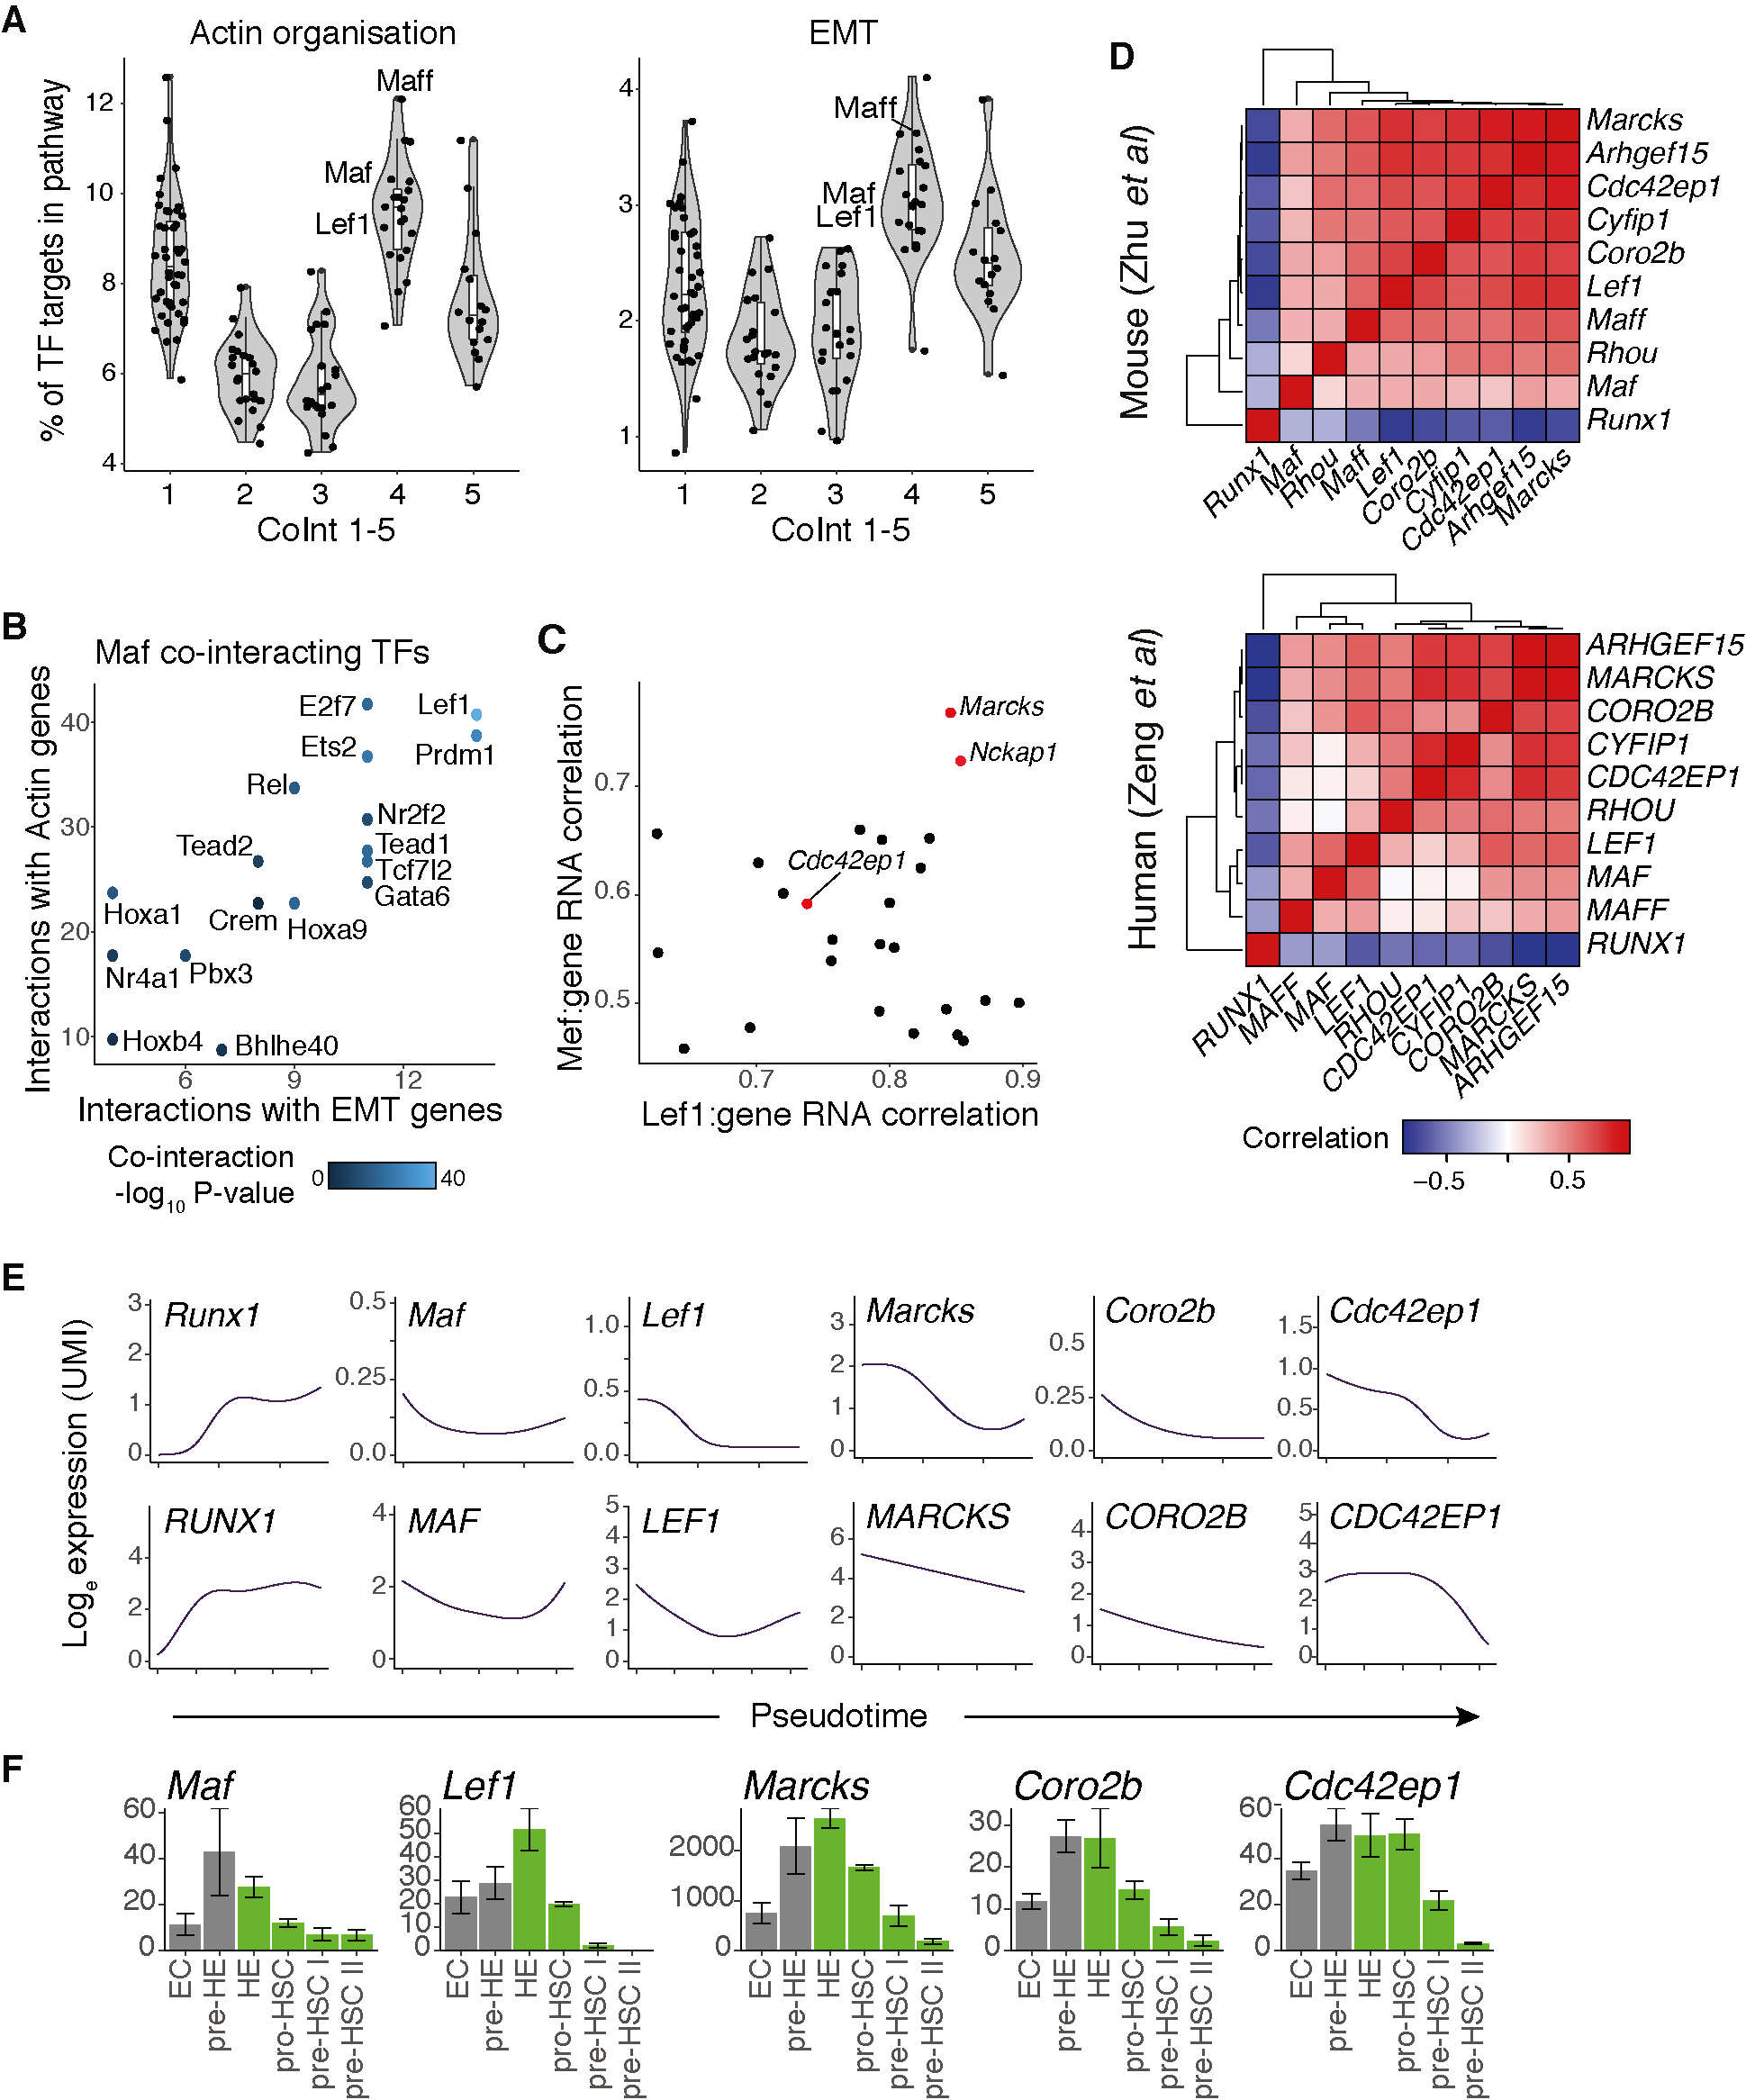
\includegraphics[width=\textwidth,height=\textheight,keepaspectratio]{figures/chapter3/ch3_maf-lef1.png}
    \caption[{The transient co-interaction module is predicted to drive cytoskeletal rearrangement through Maf:Lef1 cooperative action.}]
    {\textbf{The transient co-interaction module is predicted to drive cytoskeletal rearrangement through Maf:Lef1 cooperative action.} 
    \textbf{(A)} Proportion of TF targets that regulate actin cytoskeletal organisation (GO:0030036, left) and EMT (GO:0001837, right), across co-interaction clusters. Colour represents RNA expression modules. 
    \textbf{(B)} Frequency of TF targets regulating actin cytoskeletal organisation and EMT pathways. TFs shown significantly co-interact with Maf (FDR < 0.05). 
    \textbf{(C)} Gene expression correlation of actin cytoskeletal organisation genes, and \textit{Maf} or \textit{Lef1}. Genes of interest highlighted in red. 
    \textbf{(D)} Correlation heatmaps from scRNA-seq EHT data. 
    \textit{Legend continued on next page.}
    }
    \label{fig:ch3_maf1-lef1}
\end{figure}

There are several genes that significantly co-interact with Maf, but relatively few of these prominently interact with actin or EMT related genes (Fig. \ref{fig:ch3_maf1-lef1}B). Lef1 is a CoInt-3 TF that interacts highly with both pathways and is among the most central regulators of the transient expression module (Fig. \ref{fig:ch3_centrality}A). Of actin genes, both \textit{Maf} and \textit{Lef1} gene expression is highly correlated with \textit{Marcks} and \textit{Nckap1} expression, and moderately correlated with \textit{Cdc42ep1} (Fig. \ref{fig:ch3_maf1-lef1}C). Marcks is a membrane-bound or cytoplasmic protein that drives cytoskeletal rearrangement and migration, and has been implicated in EMT \citep{el_amri_marcks_2018, xiang_myristoylated_2019}. Cdc42ep1 (also known as Borg5) is associated with Cdc42, a key regulator of actin dynamics, and drives directional migration and angiogenesis \citep{liu_borg5_2014, farrugia_borg_2016, watson_cdc42_2016}. Nckap1 (HEM-2) is a component of the WAVE complex, which promotes activity of Arp2/3 to drive actin branching \citep{chen_structure_2010, chen_wave_2014}. To reinforce this model of Maf and Lef1 regulating actin related genes I used the EHT scRNA-seq data from \cite{zhu_developmental_2020} and \cite{zeng_tracing_2019}. Many of the actin-related genes are correlated with each other, as well as with \textit{Maf} and \textit{Lef1} expression (Fig. \ref{fig:ch3_maf1-lef1}D). Note that these scRNA-seq data consist of E9.5 and E10.5 populations, and so captures the end of EHT. Single cell pseudotime analysis shows \textit{Maf}, \textit{Lef1}, and actin genes to decrease in expression over time, in line with bulk RNA-seq expression patterns from E9.5 HE to E10.5 pre-HSC II (Fig. \ref{fig:ch3_maf1-lef1}E-F). This analysis supports a model whereby Maf1 and Lef1 cooperate to drive morphological changes, though this has yet to be experimentally validated. 
\begin{figure}[!t]
    \ContinuedFloat
    \hrule
    \vspace{5mm}
    \caption[]
    {\textit{Legend continued from previous page}. \textbf{(E)} scRNA-seq expression of \textit{Maf}, \textit{Lef1}, and key actin related genes for mouse (top) and human (bottom) over pseudotime. Lines indicate smooth fitted values calculated by TradeSeq. 
    \textbf{(F)} Gene expression (CPM) for \textit{Maf}, \textit{Lef1}, and key actin related genes in bulk RNA-seq data. Error bars represent standard error of the mean; \textit{n} = 3; \textit{n} = 4 for pre-HE. 
    \textit{Raw scRNA-seq data from \cite{zhu_developmental_2020} and \cite{zeng_tracing_2019}, reanalysed by me.} 
    }
\end{figure}
\vspace*{3in}

\clearpage
\section{Conclusions and discussion}

In this chapter, I aimed to explore potential mechanisms by which EHT regulation is driven. Through the integration of RNA-seq and ATAC-seq datasets, I have established a GRN model that predicts TF regulation that may drive activity of complex regulatory patterns associated with EHT. Using this GRN model I characterised predicted upstream regulators, and downstream targets, of Runx1. Taking advantage of these predicted interactions, I performed an analysis predicting possible TF cooperation that may drive EHT programs. One of these predicted TF cooperations was a Runx1:Ikzf1 driven FFL that represses Notch pathway genes. This FFL may contribute to deactivation of the transiently regulated EHT program, as the Hes1 motif underlies many transiently accessible enhancers (Fig. \ref{fig:ch3_runx1-TF-motifs}B).

While several studies have established GRN models of EHT \citep{baron_single-cell_2018, zhu_developmental_2020, zeng_tracing_2019, bergiers_single-cell_2018, gao_transcriptional_2020}, they do not incorporate early EHT populations in E8.5 embryos. The initiation of HE identity can be considered to occur at E8.5, with activation the 23GFP transgene in dorsal aorta endothelium \citep{swiers_early_2013}, referred to as pre-HE. 23GFP expression in pre-HE precedes endogenous \textit{Runx1} transcription, and was shown to receive pro-haemogenic signals prior to \textit{Runx1} activation. Analysis of RNA-seq data found \textit{Cd109} to be highly expressed in pre-HE and HE cells, and inactive in 23GFP- endothelium (section \ref{ch3:cd109}). The role of CD109 in EHT has not been studied, though it is known to block TGF-$\beta$ signalling \citep{mii_cd109_2019}, and therefore may act to modulate this pathway in pre-HE and HE. The role of TGF-$\beta$ signalling in EHT is unclear, as it has been shown to both inhibit \citep{vargel_activation_2016}, and promote EHT \citep{monteiro_transforming_2016}. Importantly, \cite{monteiro_transforming_2016} used morpholinos in zebrafish to perturb \textit{Tgf-$\beta$} and \textit{tgfbR2}, with no population-specific targeting, while \cite{vargel_activation_2016} treated with Tgf-$\beta$ ligand or inhibitor in mESC haematopoietic differentiations. Both studies show that either addition of TGF-$\beta$ \citep{vargel_activation_2016}, or removal of Tgf-$\beta$ \citep{monteiro_transforming_2016}, result in impaired EHT. These studies perturb Tgf-$\beta$ to either low, or higher than normal levels, which may indicate a specific dose-dependent requirement that Cd109 may function to adjust in HE. Further study is required to determine the role of CD109 in EHT, and how TGF-$\beta$ signalling is affected by its expression.

The GRN model was built through integrating multiple experimental datasets (section \ref{ch3:grn}), using a methodology with specific advantages and disadvantages. The construction of this GRN relied upon robust identification of regulatory elements, and reliable association of these elements to promoters. Due to the scarcity of HE cells in embryos, ChIP-seq data was unavailable and so enhancer histone marks (H3K27ac and H3K4me1, \cite{heintzman_histone_2009, heintzman_distinct_2007, creyghton_histone_2010}) could not be used. Additionally, while DAEs were annotated to the nearest DEG, regulatory elements are known to skip promoters to act on distal genes \citep{chepelev_characterization_2012}. These caveats were compensated for by incorporating only DEGs and DAEs, so that dynamic genes and accessible elements are incorporated, and E-P interactions were filtered for correlation between RNA-seq and ATAC-seq counts (as used in \cite{sheffield_patterns_2013, hariprakash_computational_2019}). As such, E-P interactions were enriched for elements that are likely to regulate gene expression, and as both positive and negative correlated E-P interactions were retained, these elements represent both enhancers and silencers. TF binding motif analysis was used as the basis to infer upstream regulators, which was further reinforced using transcription correlation between the TF regulator and predicted target gene. An additional caveat is TF motifs do not perfectly predict DNA binding. TF binding is multifaceted, and for example is influenced by chromatin accessibility, co-factors that alter base-pair preference, and the formation of cooperative TF complexes that adjust binding affinity \citep{morgunova_structural_2017, spitz_transcription_2012}. The core HOCOMOCO TF motif database was used to establish GRN interactions, as opposed to the full database which contains lower confidence TF PWMs, to improve the reliability of predictions. For motif enrichment analyses (as in Fig. \ref{fig:ch3_runx1-TF-motifs}), the full database was used, containing lower confidence TF PWMs, such as for Hes1. While the approach used in section \ref{ch3:grn} established a computationally robust GRN model of the overall EHT process, these caveats are important to consider and findings must be experimentally validated.

Gene expression and chromatin accessibility over EHT change dynamically, and can be clustered into distinct modules (RNA1-5 and ATAC1-5, section \ref{ch3:profiling}, Fig. \ref{fig:ch3_clusters}). These modules represent DEGs and DAEs biased towards different cell populations, and can be categorised as genes and elements that switch into active or inactive states (RNA2/ATAC2, RNA4/ATAC4, and RNA5/ATAC5), and those that are transiently activated or deactivated (RNA1/ATAC1 and RNA3/ATAC3). The transiently active module (RNA3) was found to be associated with EMT and actin cytoskeletal rearrangement processes, as well as Notch and BMP signalling pathways. Conversely, modules that switch into an active state (RNA4 and RNA5) were associated with general haematopoiesis. By integrating these modules with the GRN, key drivers of each module could be predicted (section \ref{ch3:centrality}, Fig. \ref{fig:ch3_centrality}). Degree centrality was used to predict key drivers within each module, and is known to correlate with gene essentiality in other systems \citep{hahn_comparative_2005, jeong_lethality_2001, koschutzki_centrality_2008}. This highlighted many known EHT regulators, particularly in the RNA4 module, including Runx1, Gfi1, and PU.1. Central TFs in the transiently expressed module (RNA3) included factors such as Fli1, Nfib, Tead1, and Gata3/6. Gata3 has recently been found to have an important role in aortic endothelium for EHT \citep{zaidan_endothelial-specific_2022}, which in combination with its transient expression pattern, may suggest a role in HE regulation. RNA5 TFs are expressed primarily in pre-HSC populations, and the top-most central of these factors include Ikzf1, which has not yet been extensively studied in EHT.

As Runx1 is essential for EHT, I explored both upstream and downstream regulators (section \ref{ch3:runx1-motifs} and \ref{ch3:runx1-targets}) of the TF. As the pre-HE population is characterised by 23GFP expression, it implies that factors that can regulate enhancer activity are present at this stage. There are multiple TFs with motifs found in the +23 enhancer, that are also upregulated in pre-HE over ECs, including Maf, Elk4, Klf6, Prdm16, Smad3, Sp4, and Tcf4, with \textit{Maf} expression being particularly biased towards pre-HE. At transitions where \textit{Runx1} is upregulated (pre-HE to HE, and HE to pro-HSC), we find several TFs concurrently upregulated in these transitions, with motifs at \textit{Runx1} enhancers. For example, NFI motifs underly -59 and +24 enhancers, and Nfib is a highly central RNA3 TF. Data from the de Bruijn lab (unpublished) found the +24 element to have little enhancer activity on its own, but boosted the activity of the +23 enhancer, so Nfib may act to support +23 enhancer activity. Additionally, CEBP motifs were found specifically in the +110 enhancer, and AP-1 motifs specifically in the +204 enhancer, highlighting the potential differences between regulatory elements. 

\begin{figure}[t]
    \centering
    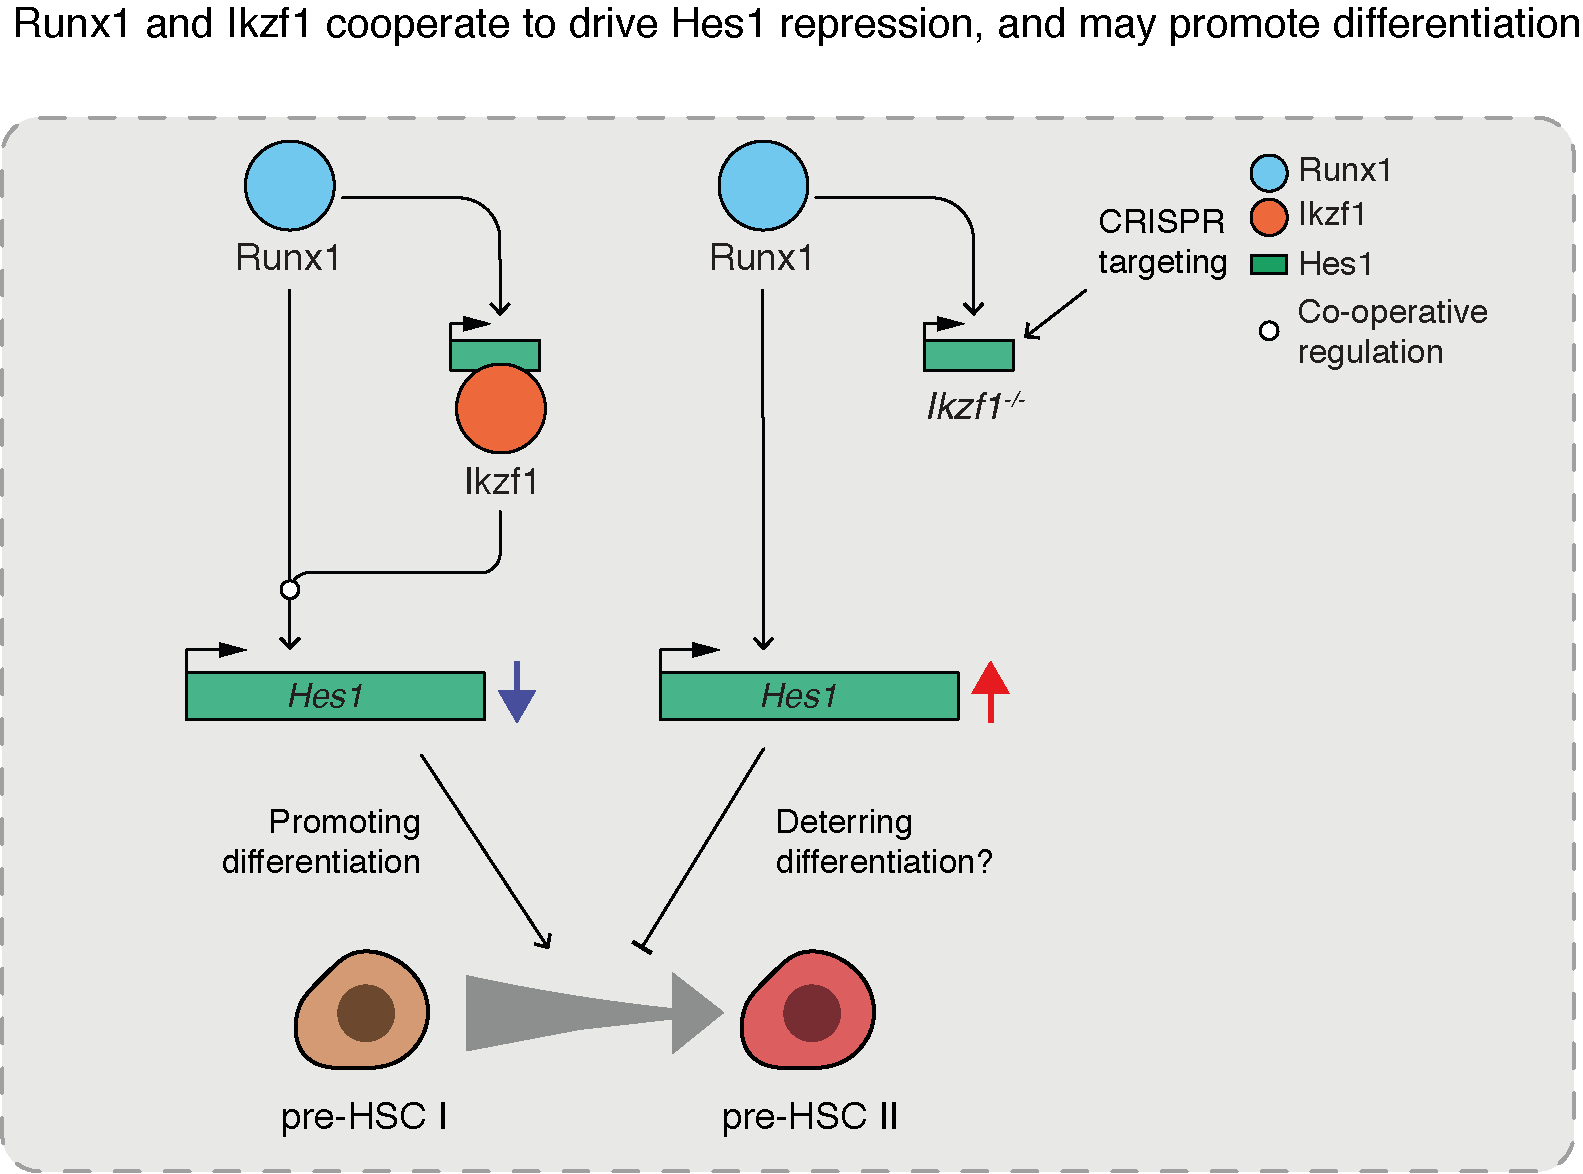
\includegraphics[width=\textwidth,height=\textheight,keepaspectratio]{figures/models/ch3_model-runx1-ikzf1-hes1.png}
    \caption[{Summary model of Runx1 and Ikzf1 cooperation to drive \textit{Hes1} repression.}]
    {\textbf{Summary model of Runx1 and Ikzf1 cooperation to drive \textit{Hes1} repression.}
    A model of a Runx1 and Ikzf1 driven FFL, predicted to drive \textit{Hes1} repression. Runx1 and Ikzf1 appear to cooperate at the \textit{Hes1} locus. Where Runx1 and Ikzf1 are predicted to cooperate and drive repression, in \textit{Ikzf1\textsuperscript{-/-}} conditions Runx1 may instead upregulate \textit{Hes1}. As repression of the Notch pathway is required for the pre-HSC I to pre-HSC II transition \citep{souilhol_developing_2016}, this may be an important circuit for the progression of late-EHT maturation. 
    }
    \label{fig:ch3_model-runx1-ikzf1-hes1}
\end{figure}

One aspect of gene regulation that remains challenging to study, is the cooperative action of TFs to regulate genes. TFs can often act in complexes, resulting in changes in their activity or shifting DNA binding sequence preference. Runx1 is known to cooperate with multiple TFs \citep{wang_intersection_2011, zaidi_integration_2002, hu_runx1_2011, kim_mutual_1999, goetz_auto-inhibition_2000, lichtinger_runx1_2012}. I explored TFs that frequently co-interact with Runx1 at enhancers and promoters (section \ref{ch3:co-interaction}), suggesting that Runx1 may cooperate with these factors to co-regulate genes. Among the TFs most frequently co-interacting with Runx1 was Ikzf1, a highly central regulator in the RNA5 expression module. \textit{Ikzf1} was also found to be a target of Runx1 (section \ref{ch3:runx1-targets}, Fig. \ref{fig:ch3_pairwise}). While \textit{Ikzf1} was expressed in pre-HSC populations, IKZF1 motifs were found primarily in transiently accessible elements (ATAC3, section \ref{ch3:notch}, Fig. \ref{fig:ch3_runx1-TF-motifs}). The GRN analysis predicted Runx1 and Ikzf1 to repress the transiently active Notch pathway (RNA3, ATAC3) in a FFL configuration, and experiments performed by L. Greder (de Bruijn lab, unpublished) supported these factors to repress \textit{Hes1} expression (Fig. \ref{fig:ch3_model-runx1-ikzf1-hes1}, Appendix \ref{fig:app_notch-ffl-validation}). Interestingly, these experiments found that in the absence of Ikzf1, Runx1 appeared to upregulate \textit{Hes1} expression. In the presence of Ikzf1, Runx1 instead represses \textit{Hes1} expression. This could suggest that the activity of Runx1 changes, depending on the presence of Ikzf1. One possible explanation for this is that Runx1 and Ikzf1 may physically interact, resulting in a change in Runx1 activity. A previous study has found human IKZF1 to physically interact with RUNX1 protein \citep{zhou_runx_2019}, supporting this hypothesis. An alternative explanation is that Ikzf1 activity takes precedence, and as Runx1 drives \textit{Ikzf1} expression, there may be higher levels of Ikzf1 in Ikzf1+/Runx1+ conditions resulting in greater \textit{Hes1} downregulation. These functional analyses support a mechanism by which Runx1 and Ikzf1 repress Notch pathway genes in pre-HSC I and pre-HSC II, though further study is necessary to elucidate the molecular mechanism behind Runx1 and Ikzf1 cooperation. Importantly, repression of the Notch pathway is a required step for the progression of pre-HSC I to pre-HSC II cells \citep{souilhol_developing_2016}, placing this Runx1:Ikzf1:\textit{Hes1} FFL as a potentially important circuit for driving differentiation of late EHT populations (Fig. \ref{fig:ch3_model-runx1-ikzf1-hes1}).

The analytical strategy for exploring TF co-interaction was also applied to study the regulation of EMT and actin cytoskeletal organisation pathways, in order to investigate the processes underlying the morphological changes that occur during EHT (section \ref{ch3:maf-lef1}). This preliminary analysis identified Maf and Lef1 as two TFs that were predicted to regulate many genes in these pathways, and these were found to frequently co-interact at the same accessible elements. These factors were also highly correlated with several actin cytoskeleton genes, particularly \textit{Marcks}. The Marcks protein drives cytoskeletal rearrangement, resulting in cell migration and EMT \citep{el_amri_marcks_2018, xiang_myristoylated_2019}, placing it as a candidate driver of EHT morphological changes. Maf and Lef1 were also predicted to regulate Cdc42ep1 (Borg5), which associates with an important driver of cell migration, Cdc42 \citep{liu_borg5_2014, farrugia_borg_2016, watson_cdc42_2016}. This places both Maf and Lef1 as possible drivers of cytoskeletal machinery, and may contribute to the budding process during EHT. Further study is required to validate these interactions, and determine whether Maf1 and Lef1 functionally cooperate, and whether their activity is required for EHT.

% regarding pairwise:
%Well known hematopoietic factors are activated early in EHT between EC and pre-HE, including as \textit{Meis1} \citep{pineault_differential_2002}, \textit{Nkx2-3} \citep{nagel_nkl_2017}, and \textit{CD109} \citep{murray_cd109_1999}. 
%The small number of upregulated genes in these late-EHT transitions are strongly associated with a HSPC profile, such as \textit{Ptprc} (CD45) \citep{taoudi_extensive_2008}, \textit{Rac2} \citep{gu_hematopoietic_2003, shang_r-ras_2011}, and \textit{Cd69} \citep{testi_cd69_1994}, and are enriched for T cell and lymphocyte activation terms. 

\chapter{\label{chapter4_MA4}MLL-AF4 and RUNX1 driven regulatory networks in \textit{MLL}r leukaemia}
\chaptermark{Chapter 4 - MLL-AF4 GRN}

\begingroup
\raggedright
\minitoc
\endgroup

\clearpage % Keep contents seperate page

% Put declaration here?!

\section{Introduction and aims}

In chapter \ref{chapter3_EHT} I established a GRN model of mouse EHT. This is a normal haematopoietic process, describing the differentiation of aortic endothelium towards HSCs. I focused the analysis of this model on the activity of Runx1, and I used an analytical approach to predict possible TF cooperation. For this chapter, I asked how abnormal haematopoiesis may be regulated. MLL-AF4 leukaemias are considered a transcriptional disease, as the translocation event can be sufficient on its own for leukaemogenesis, with few or no cooperative mutations \citep{bardini_dna_2010, bardini_implementation_2011, the_cancer_genome_atlas_research_network_genomic_2013, andersson_landscape_2015}. As described in section \ref{ch1:mll-af4-function}, MLL-AF4 binds to gene promoters and drives transcription through the recruitment of a large transcription elongation complex \citep{ballabio_molecular_2012, slany_mll_2020}. This makes \textit{MLL}r leukaemias particularly suited for analysis using GRN methods, which rely on transcriptional data. Additionally, the MLL-AF4 fusion protein maintains overexpressed \textit{RUNX1} expression \citep{wilkinson_runx1_2013}, which allows for the study of dysregulated RUNX1 activity in a leukaemic network context.

\begin{figure}[!t]
    \centering
    %\includegraphics[width=\textwidth,height=\textheight,keepaspectratio]{figures/chapter4/ch1_grn-justification.png}
    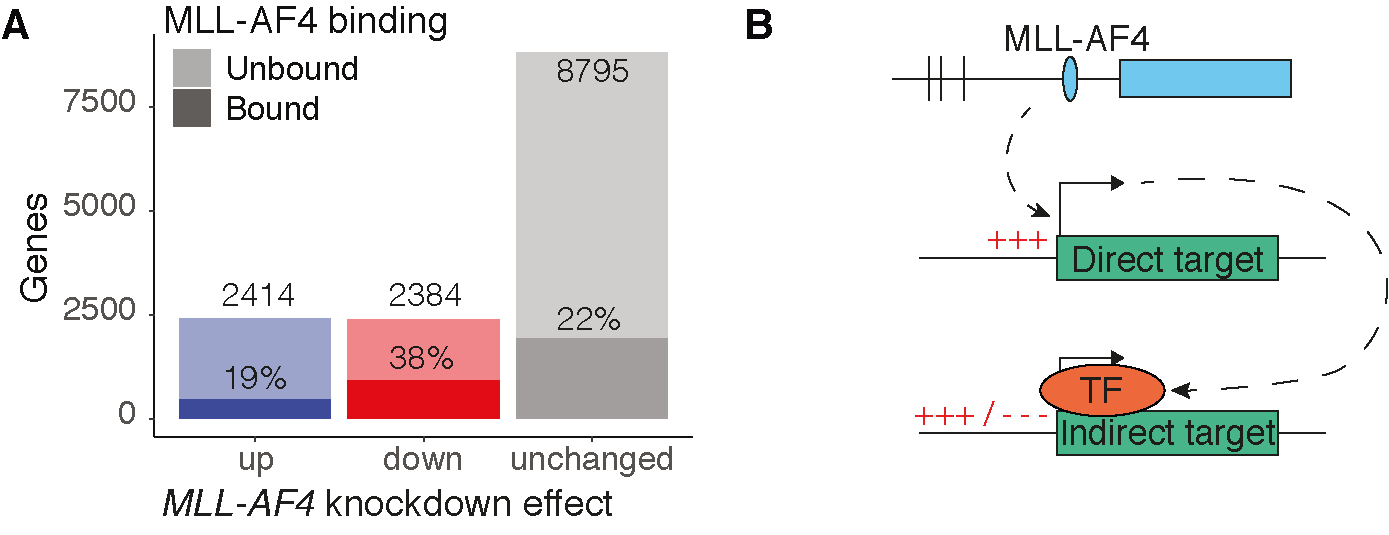
\includegraphics{figures/chapter4/ch4_grn-justification.png}
    \caption[{MLL-AF4 regulation cannot be explained by direct binding alone.}]
    {\textbf{MLL-AF4 regulation cannot be explained by direct binding alone.} 
    \textbf{(A)} Number of DEGs after 96 h \textit{MLL-AF4} KD in SEM cells (\textit{n} = 3). Shaded bar represents proportion of DEGs bound by MLL-AF4 (ChIP-seq). 
    \textbf{(B)} Schematic illustrating hypothesis, where MLL-AF4 regulates TFs, which then regulate additional targets, resulting in indirect downstream regulation. 
    \textit{Analysis in A first performed by R. Thorne. Adapted from \cite{harman_kmt2a-aff1_2021}.}
    }
    \label{fig:ch4_GRN_just}
\end{figure}

As the MLL-AF4 complex directly promotes transcription \citep{ballabio_molecular_2012, biswas_function_2011, kerry_mll-af4_2017, mueller_role_2007, yokoyama_higher-order_2010, lin_aff4_2010, okuda_af4_2015} and is the main driver of leukaemogenesis, it is expected that \textit{MLL-AF4} KD would lead to downregulation of gene expression, with affected genes bound by MLL-AF4 protein. Previous analysis by R. Thorne (Milne lab) of nascent RNA-seq following \textit{MLL-AF4} KD \citep{godfrey_mll-af4_2017} in the SEM cell line (B-ALL MLL-AF4, \cite{greil_acute_1994}) established that this is not true. Only 28\% of \textit{MLL-AF4} KD sensitive genes were bound by MLL-AF4, and both up- and downregulation was observed (Fig. \ref{fig:ch4_GRN_just}A, \cite{harman_kmt2a-aff1_2021}). To explain this discrepancy, I hypothesised these non-bound genes are indirectly regulated via intermediate TFs that are overactivated as a consequence of MLL-AF4 activity (Fig. \ref{fig:ch4_GRN_just}B). As TFs often do not act in isolation \citep{morgunova_structural_2017, spitz_transcription_2012}, it is important to address the possibility that MLL-AF4 may function in combination with other TFs to regulate gene targets, and thus understand the full regulatory scope of MLL-AF4. As such, a GRN model of MLL-AF4 leukaemia was established to decode complex combinatorial signals and organise direct and indirect regulatory logic, by isolating common network motifs such as FFLs and TF cascades. 

\noindent
\textbf{Aims} 

\vspace*{-5mm}
\begin{enumerate}
    \item To determine if MLL-AF4 controls a wider transcriptional network through TF activation. 
    \item To determine whether the MLL-AF4 GRN can be used to identify novel biology of MLL-AF4 leukaemias.
    \item To investigate the TF cooperativity between MLL-AF4, RUNX1, and its target TFs.
\end{enumerate}

\vspace*{-5mm}
By constructing a GRN model of MLL-AF4 leukaemia, the regulatory logic downstream of MLL-AF4 can be explored. This allows us to address the hypothesis that MLL-AF4 regulates targets indirectly via intermediate TFs. It is important to determine whether the GRN can describe the biology of leukaemia, and its relevance to real-world patient samples. As in chapter 3, a dissection of how MLL-AF4 and RUNX1 cooperate with other TFs will explore into a less studied area of gene regulation, and could offer insight into the role of intermediate TFs in MLL-AF4 leukaemia.

\clearpage


\section{\label{ch4:grn}Generating and characterising a GRN model of MLL-AF4 driven leukaemia}

To determine whether MLL-AF4 was able to control the expression of a wider transcriptional network by activating TFs, I sought to integrate nascent RNA-seq and ChIP-seq datasets generated in SEM cells (B-ALL MLL-AF4) to establish a GRN model. MLL-AF4 DNA binding is not well predicted through specific motifs. The part of MLL-AF4 that contacts DNA is the CxxC domain which confers binding preference for uCpGs \citep{birke_mt_2002}. However, MLL-AF4 only binds to a subset uCpGs and it is unknown what guides this preference \citep{kerry_mll-af4_2017}. As such, MLL-AF4 ChIP-seq \citep{kerry_mll-af4_2017} was used as evidence for direct binding, while nascent RNA-seq following 96 hours' \textit{MLL-AF4} KD \citep{kerry_mll-af4_2017} was used to identify the regulatory scope of MLL-AF4, including indirect targets. 

\begin{figure}[htbp]
    \centering
    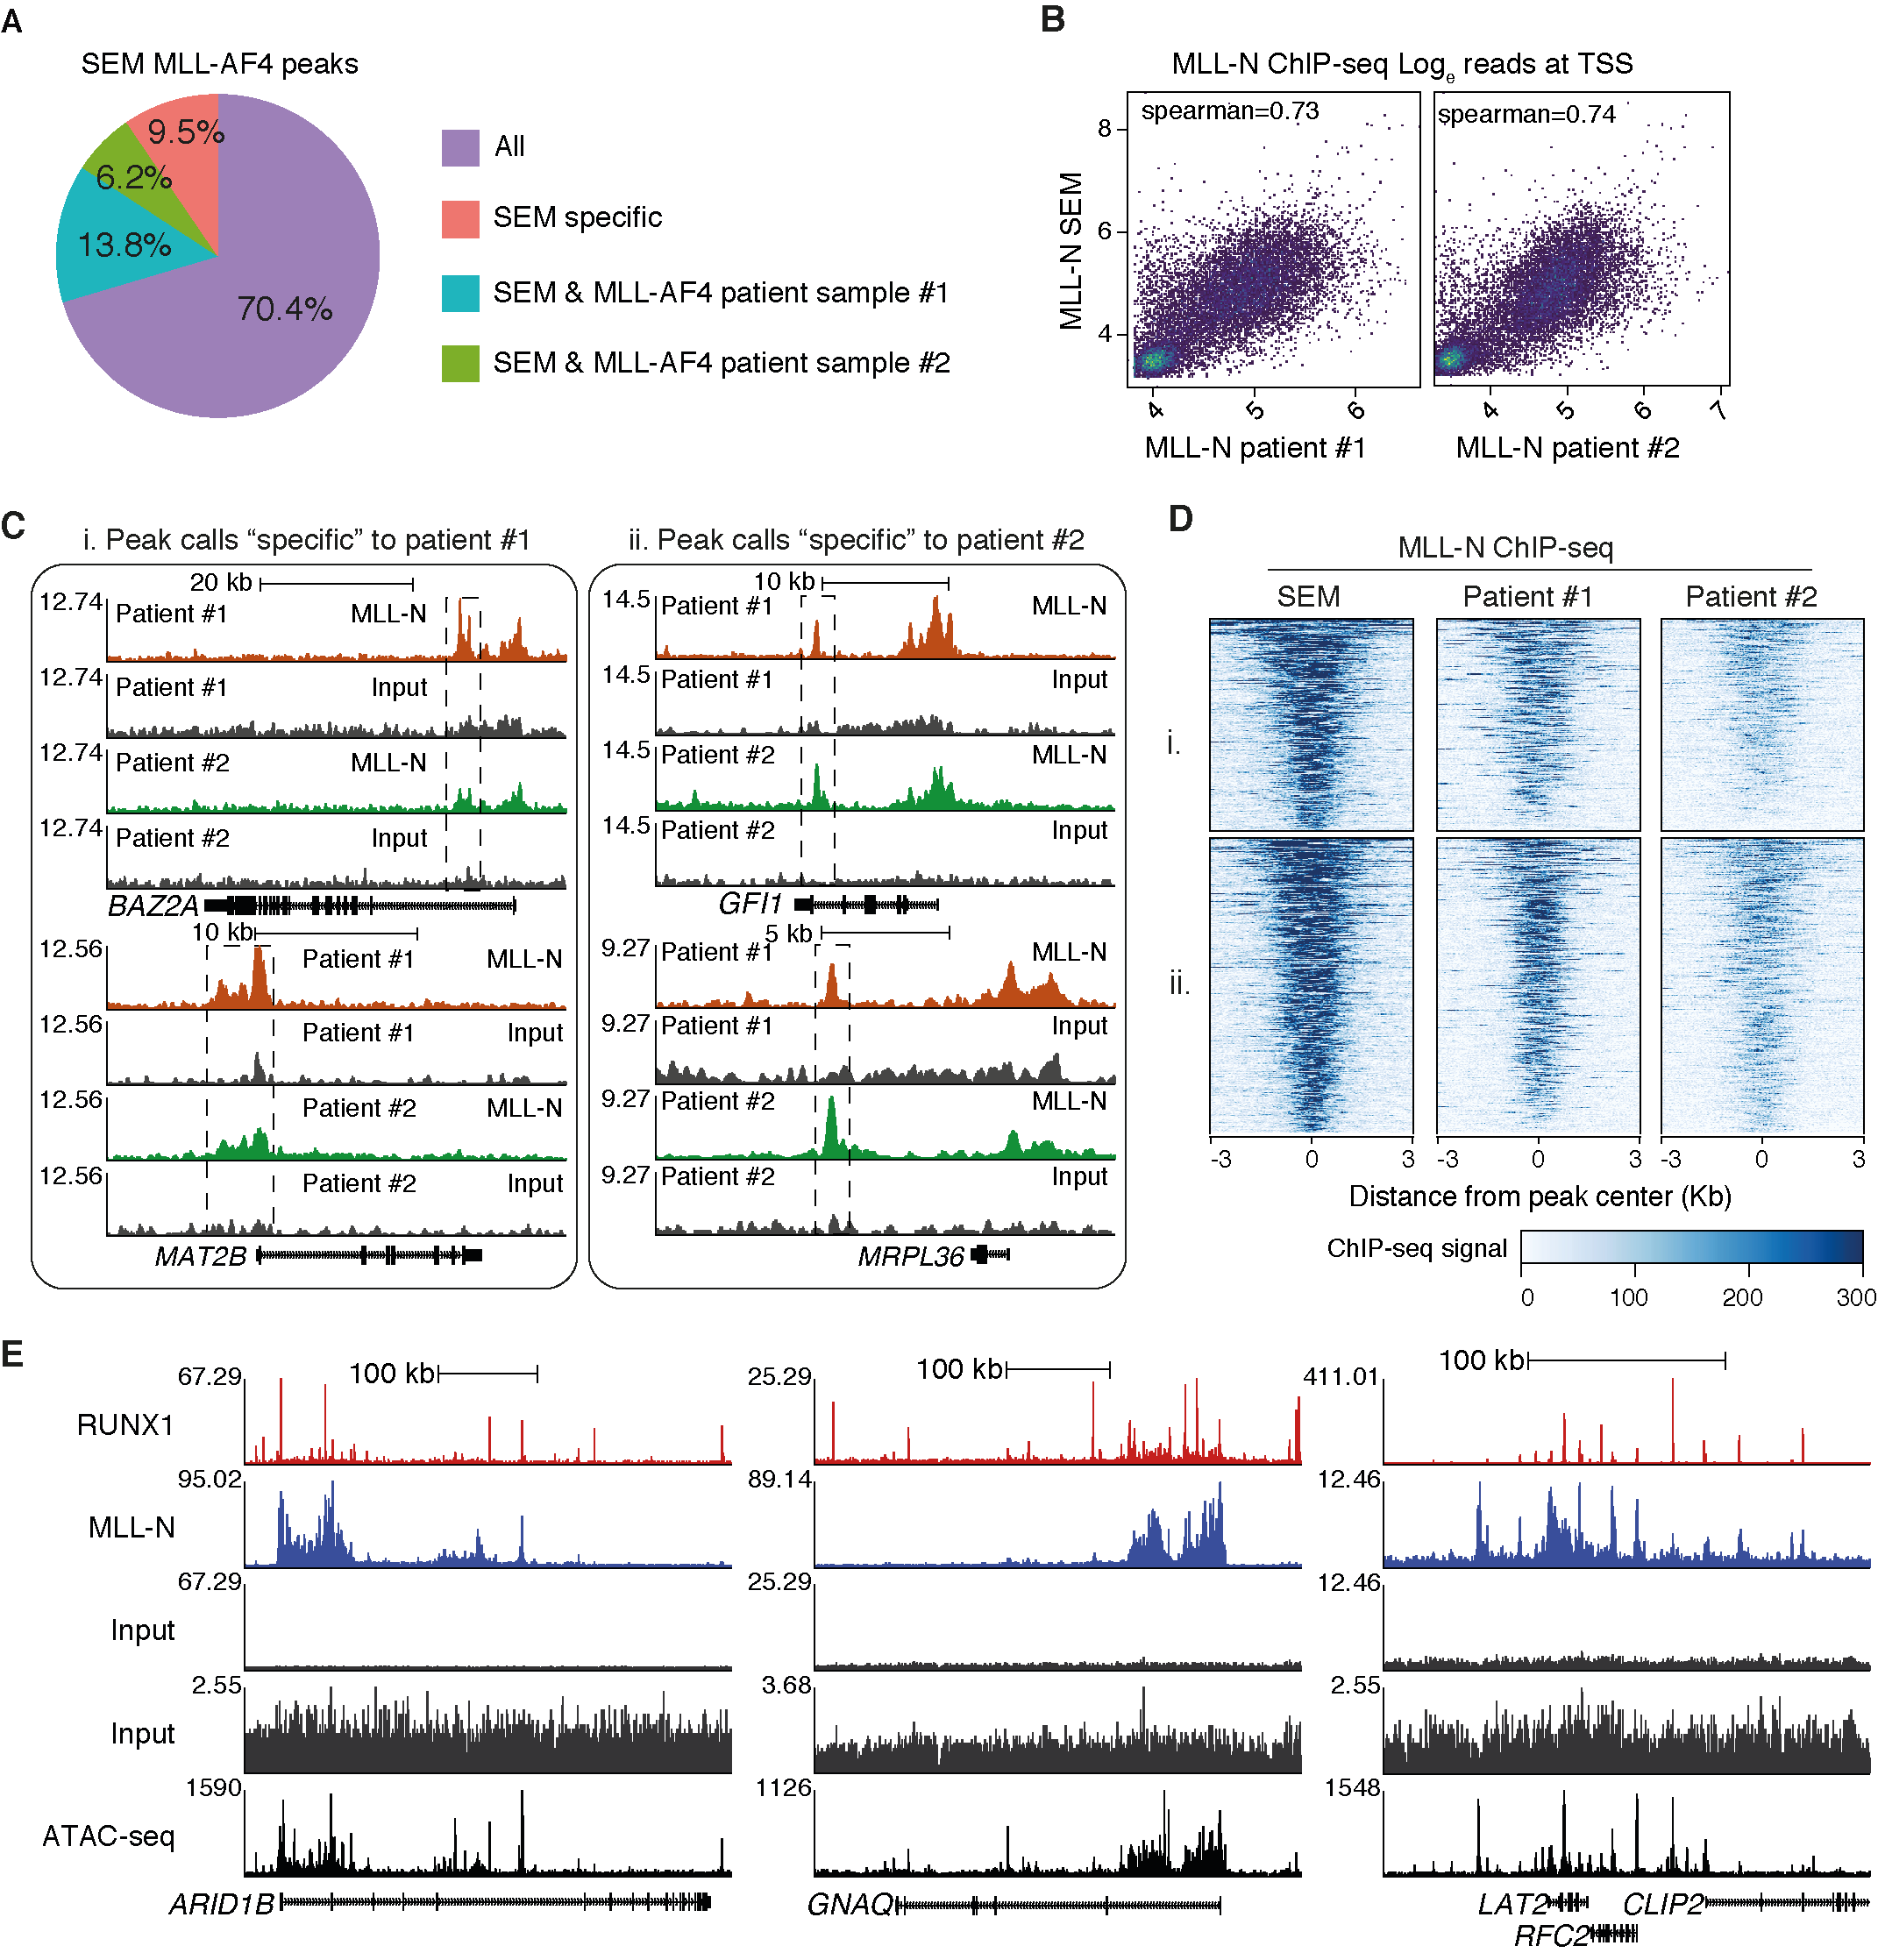
\includegraphics[width=\textwidth,keepaspectratio]{figures/chapter4/ch4_peak-qc.png}
    %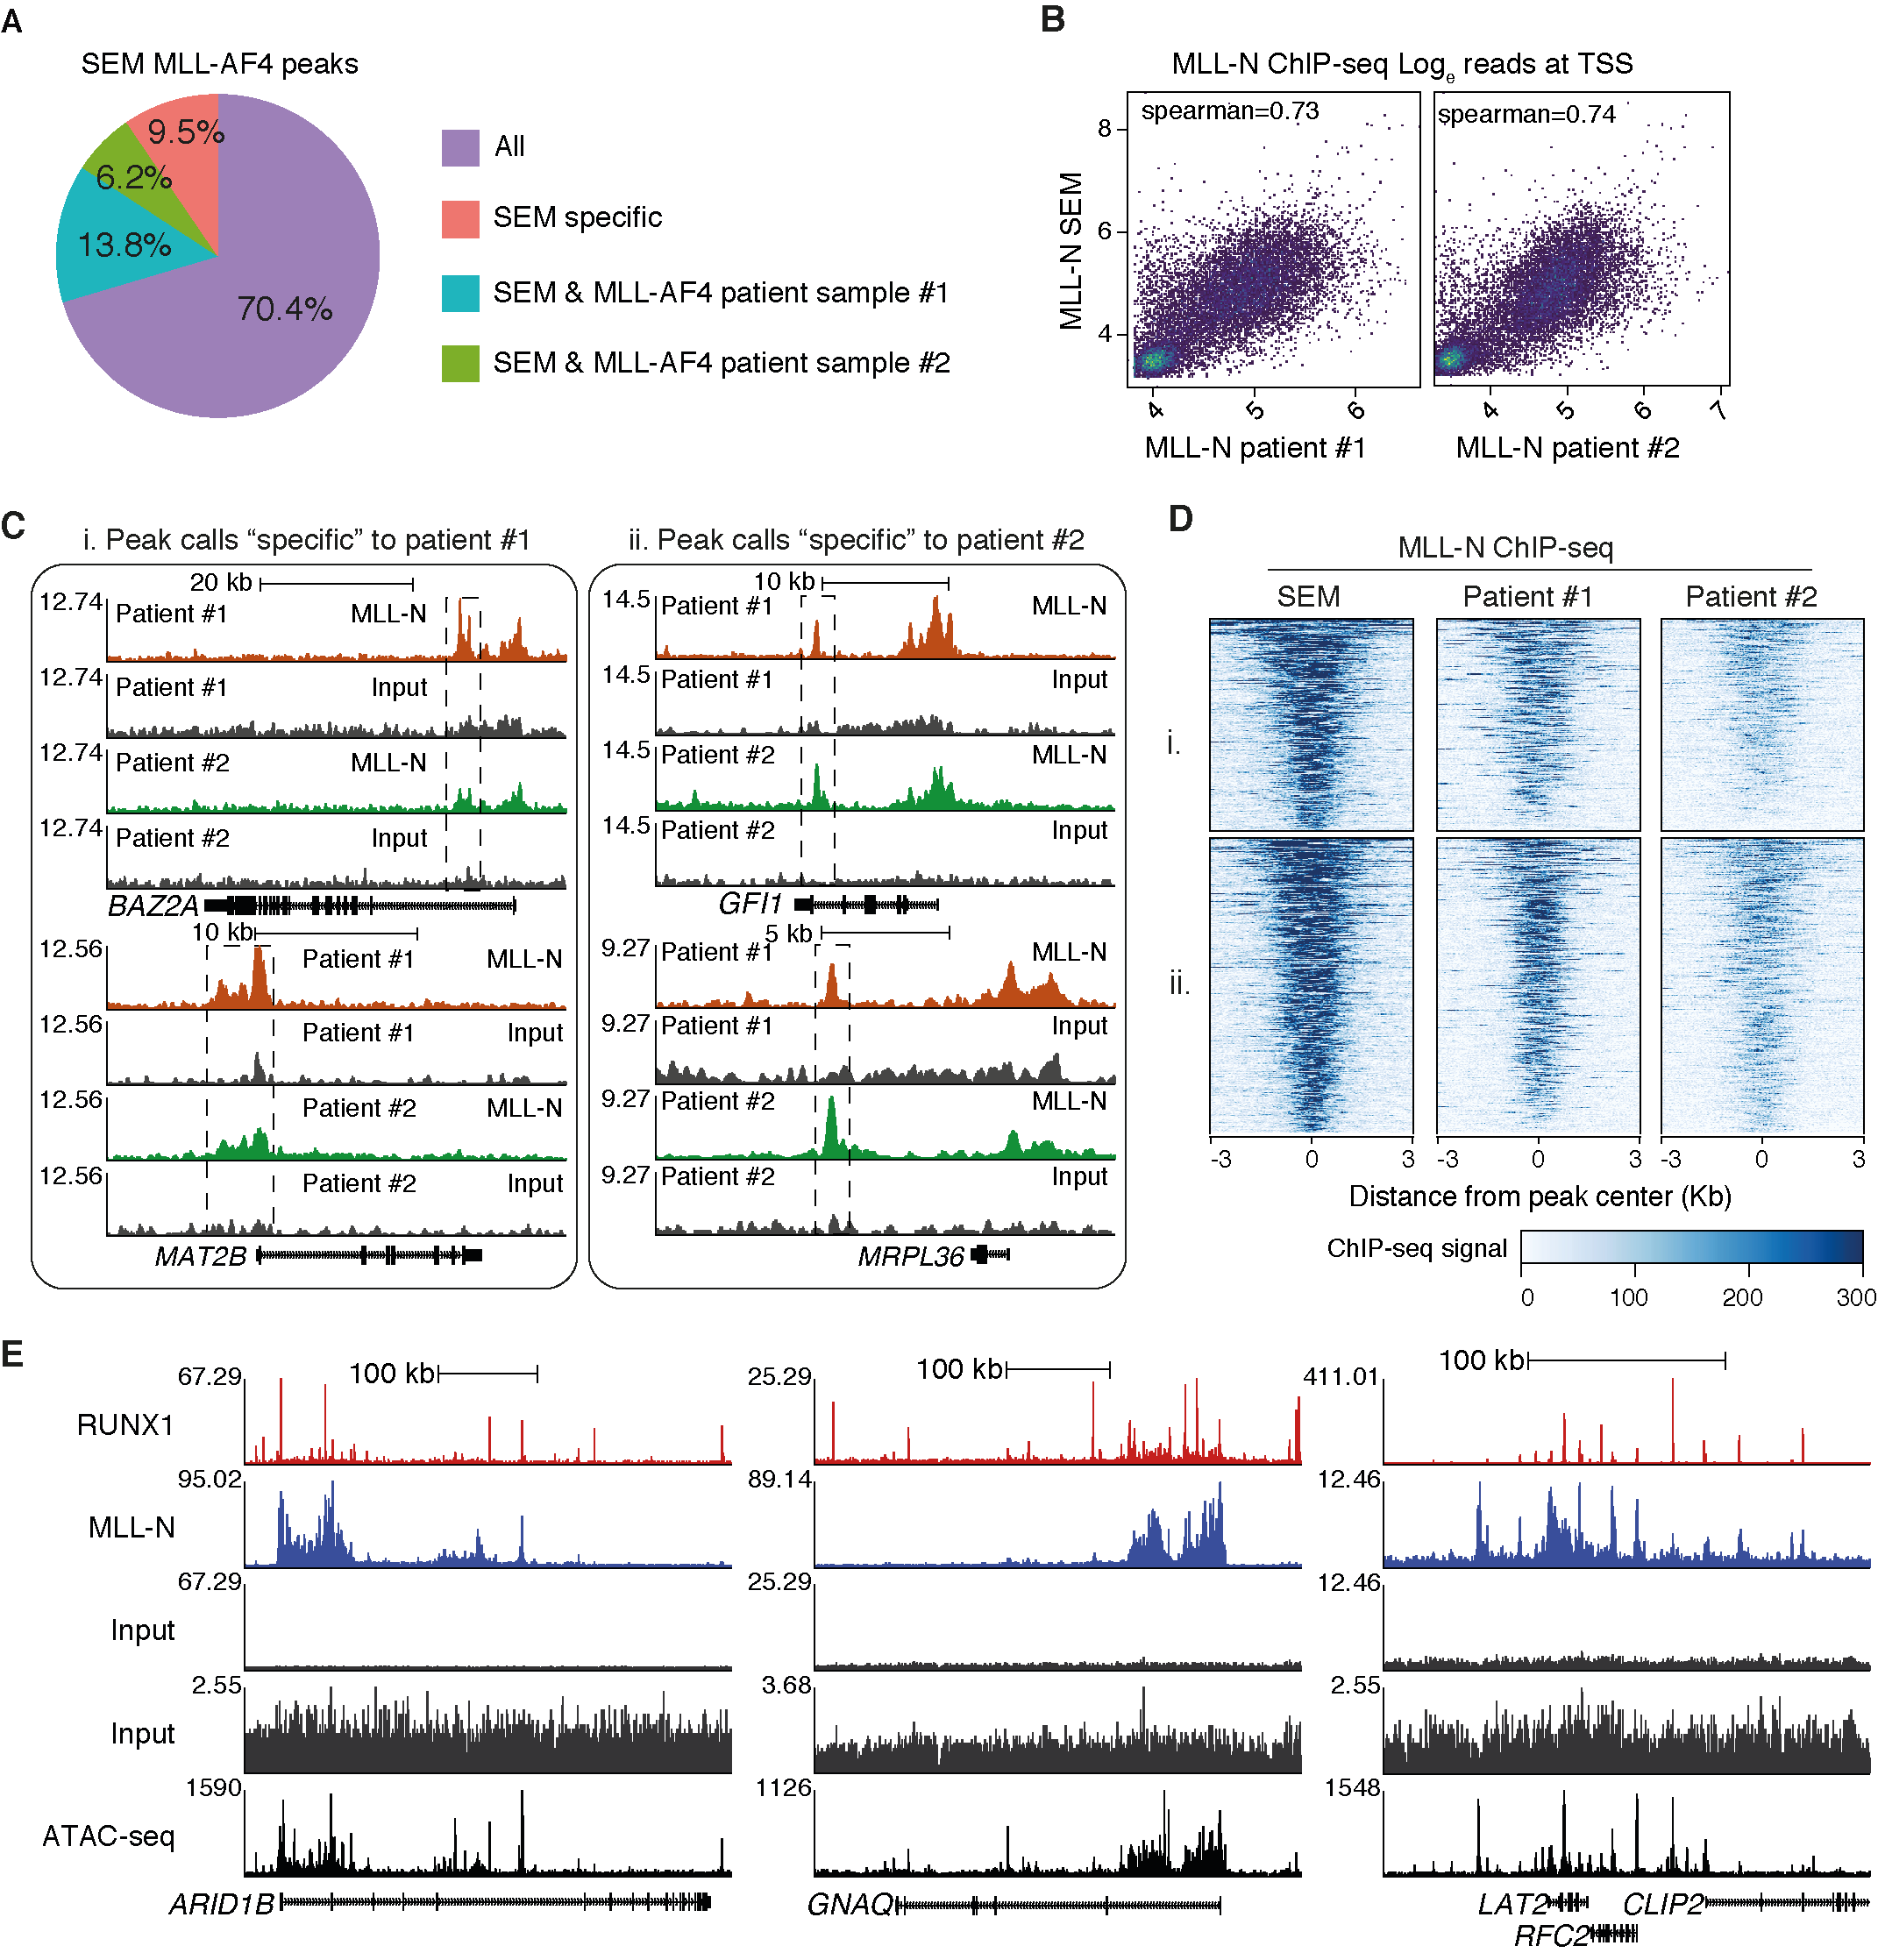
\includegraphics{figures/chapter4/ch4_peak-qc.png}
    \caption[{ChIP-seq data is of sufficient quality for GRN analysis.}]
    {\textbf{ChIP-seq data is of sufficient quality for GRN analysis.} 
    \textbf{(A)} Proportion of MLL-AF4 peaks in SEM cells that overlap with MLL-AF4 peaks in patient samples. 
    \textbf{(B)} Comparison of Log\textsubscript{e} MLL-N reads at gene promoters in SEM cells and patient samples. 
    \textbf{(C)} ChIP-seq tracks for MLL-N and input chromatin. Loci are MLL-AF4-bound genes unique to patient \#1 (i) or patient \#2 (ii), as defined in A. Boxed regions indicate peak calls of interest. 
    \textbf{(D)} ChIP-seq heatmaps for MLL-N. Loci are SEM MLL-N peaks with peak calls unique to patient \#1 (i) or patient \#2 (ii). 
    \textbf{(E)} ChIP-seq tracks for MLL-N, RUNX1, and input chromatin, and ATAC-seq from SEM cells. Input tracks are shown scaled to maximum signal, or to the lowest track height in RUNX1 or MLL-N ChIP-seq. RUNX1 and MLL-AF4 samples share input chromatin. 
    \textit{Patient MLL-N ChIP-seq generated by N. Crump, analysed by me. Adapted from \cite{harman_kmt2a-aff1_2021}.}
    }
    \label{fig:ch4_peak-qc}
\end{figure}

To establish a robust GRN, it was important that the MLL-AF4 ChIP-seq in the SEM cell line model be of sufficient quality for reliable peak calling, and representative of MLL-AF4 binding profiles in patients. To test this, I compared MLL-AF4 binding in the SEM cell line with bound genes in two MLL-AF4 ALL patient samples. The majority of peaks were common to all three samples (70.4\%) with only 9.5\% of peaks unique to SEM cells (Fig. \ref{fig:ch4_peak-qc}A), and ChIP-seq signal showed high correlation at gene promoters (Fig. \ref{fig:ch4_peak-qc}B). Some differences in MLL-AF4 bound genes were observed between the patients (13.8\% and 6.2\% of SEM bound genes only bound in patient \#1 or \#2, respectively, Fig. \ref{fig:ch4_peak-qc}A), however this is mostly due to lack of precision with peak calling where MLL-N ChIP-seq signal is weak and there are biases in input tracks (Fig. \ref{fig:ch4_peak-qc}C-D). Little bias is observed in input tracks for SEM MLL-AF4 or RUNX1 ChIP-seq (Fig. \ref{fig:ch4_peak-qc}E). From these analyses, the ChIP-seq data in SEM cells is a good representation of MLL-AF4 binding in patient samples.

To establish the MLL-AF4 GRN (methods section \ref{ch2:ma4-grn}, p.\pageref{ch2:ma4-grn}) I integrated \textit{MLL-AF4} KD DEGs, SEM MLL-AF4 ChIP-seq, and an existing TF interaction network \citep{the_fantom_consortium_and_the_riken_omics_science_center_transcriptional_2009} (Fig. \ref{fig:ch4_ma4-grn}A, B). This TF interaction network was generated in THP-1 cells (an MLL-AF9 cell line) using deepCAGE sequencing to estimate motif activity. Note that while this underlying network was generated in MLL-AF9 leukaemia we hypothesised that different MLL-FPs would target similar genes, and as such is a sufficient representation of MLL-AF4 biology. The overlap between MLL-AF4 and MLL-AF9 interactions is discussed later in this chapter (See Fig. \ref{fig:ch4_sem-thp1}). In brief, DEGs from \textit{MLL-AF4} KD were considered to represent the limits of the larger network, and ChIP-seq data was used to connect direct targets of MLL-AF4. The TF interaction network supplemented the ChIP-seq profiles and bridged direct interactions to indirect targets, generating an information rich network of potential regulators. 

\begin{figure}[ht]
    \centering
    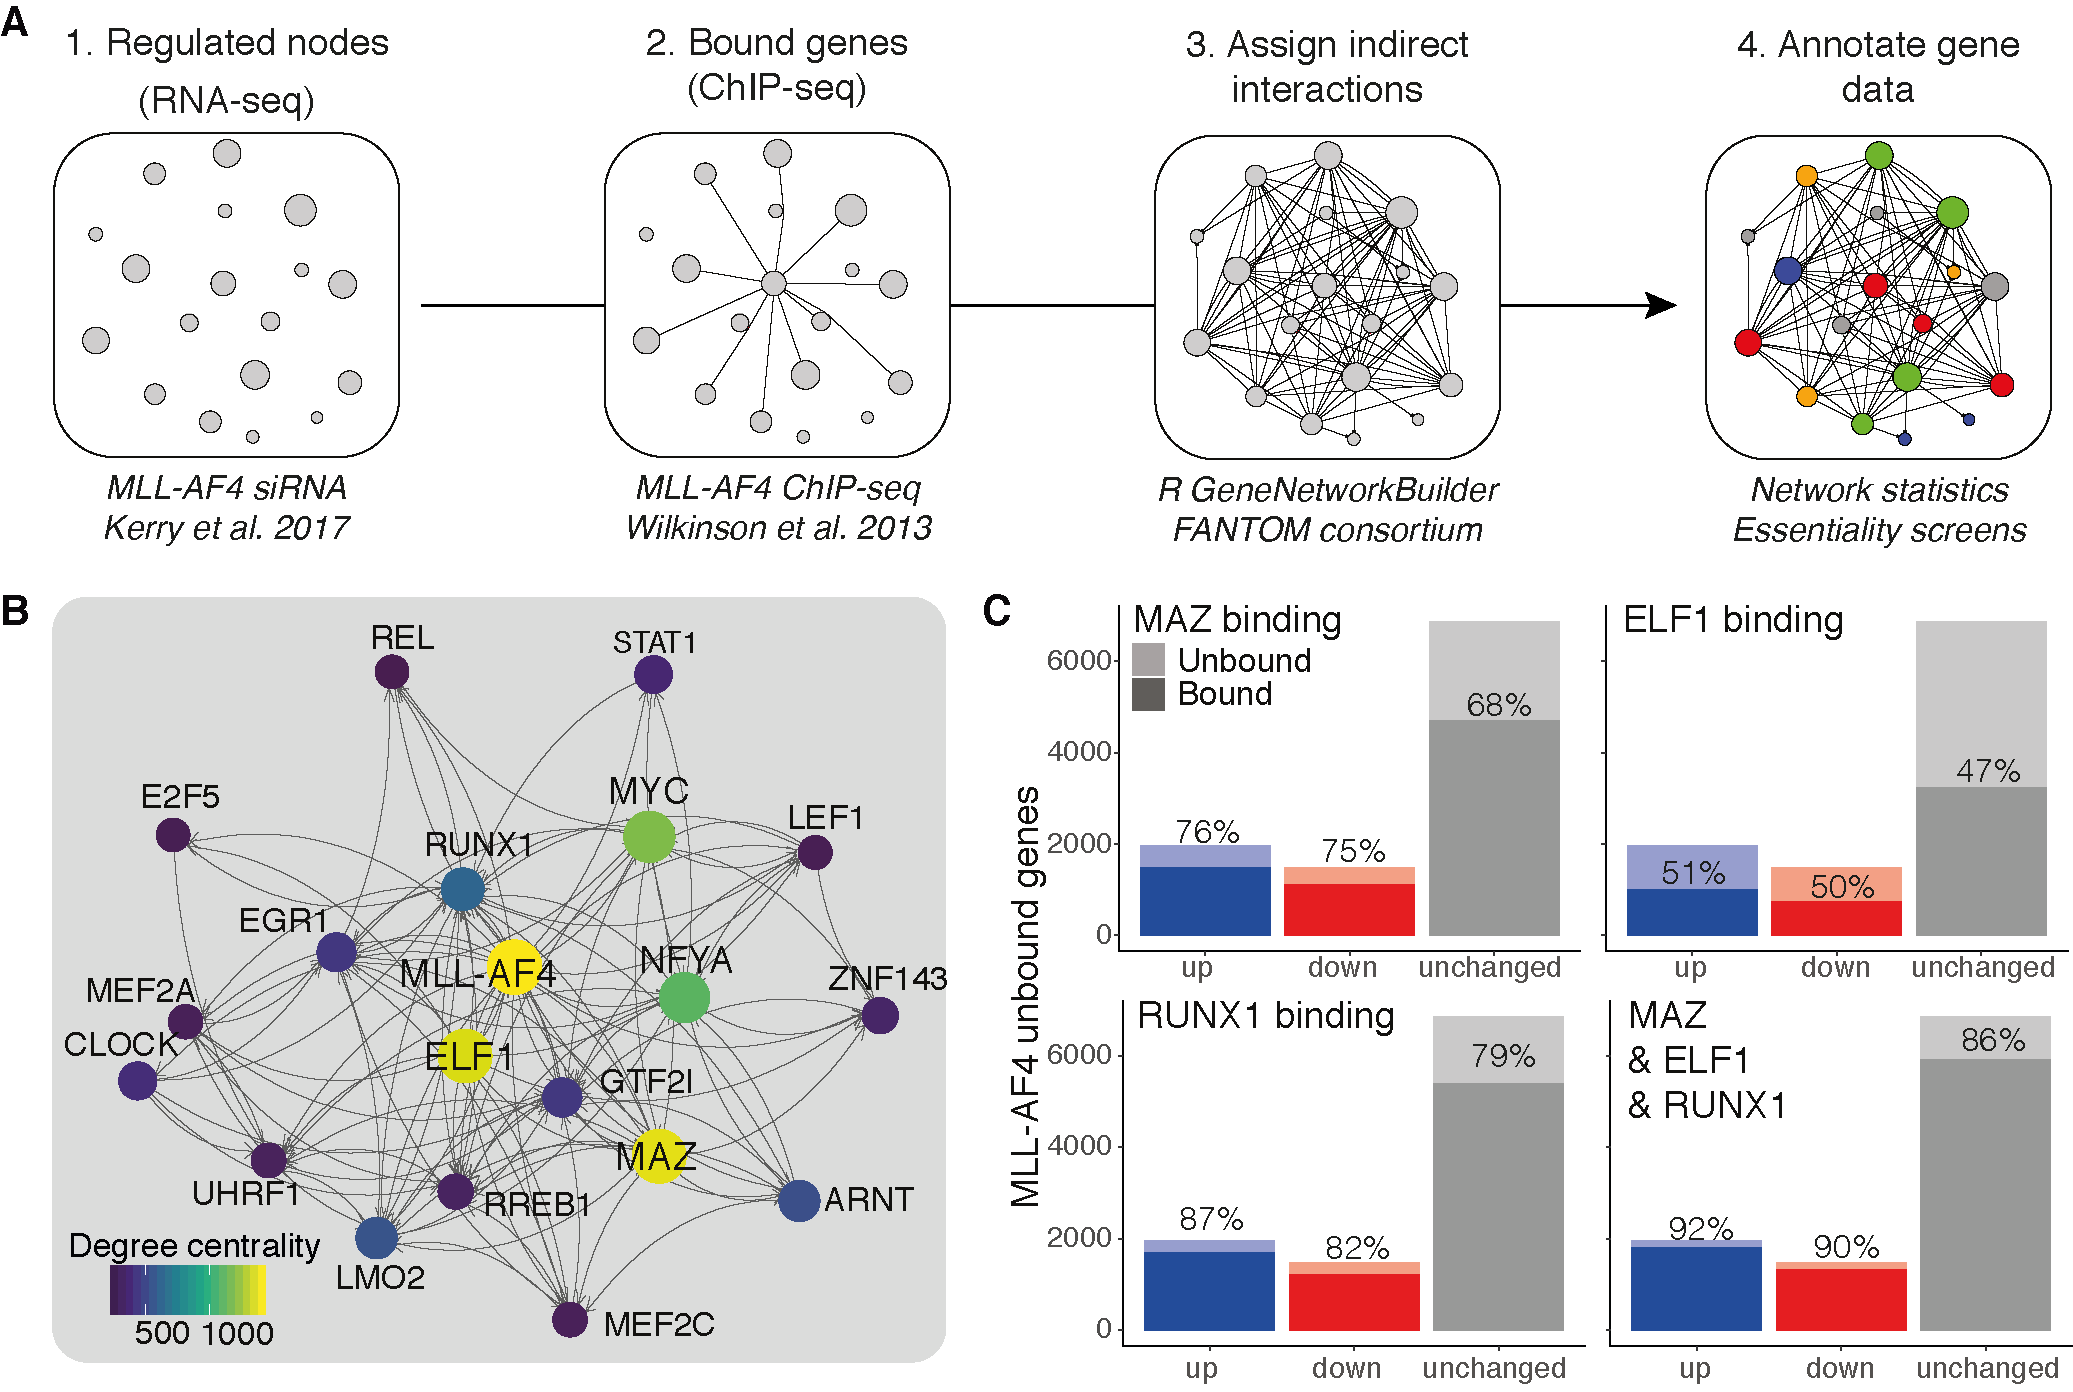
\includegraphics[width=\textwidth,height=\textheight,keepaspectratio]{figures/chapter4/ch4_ma4-grn.png}
    %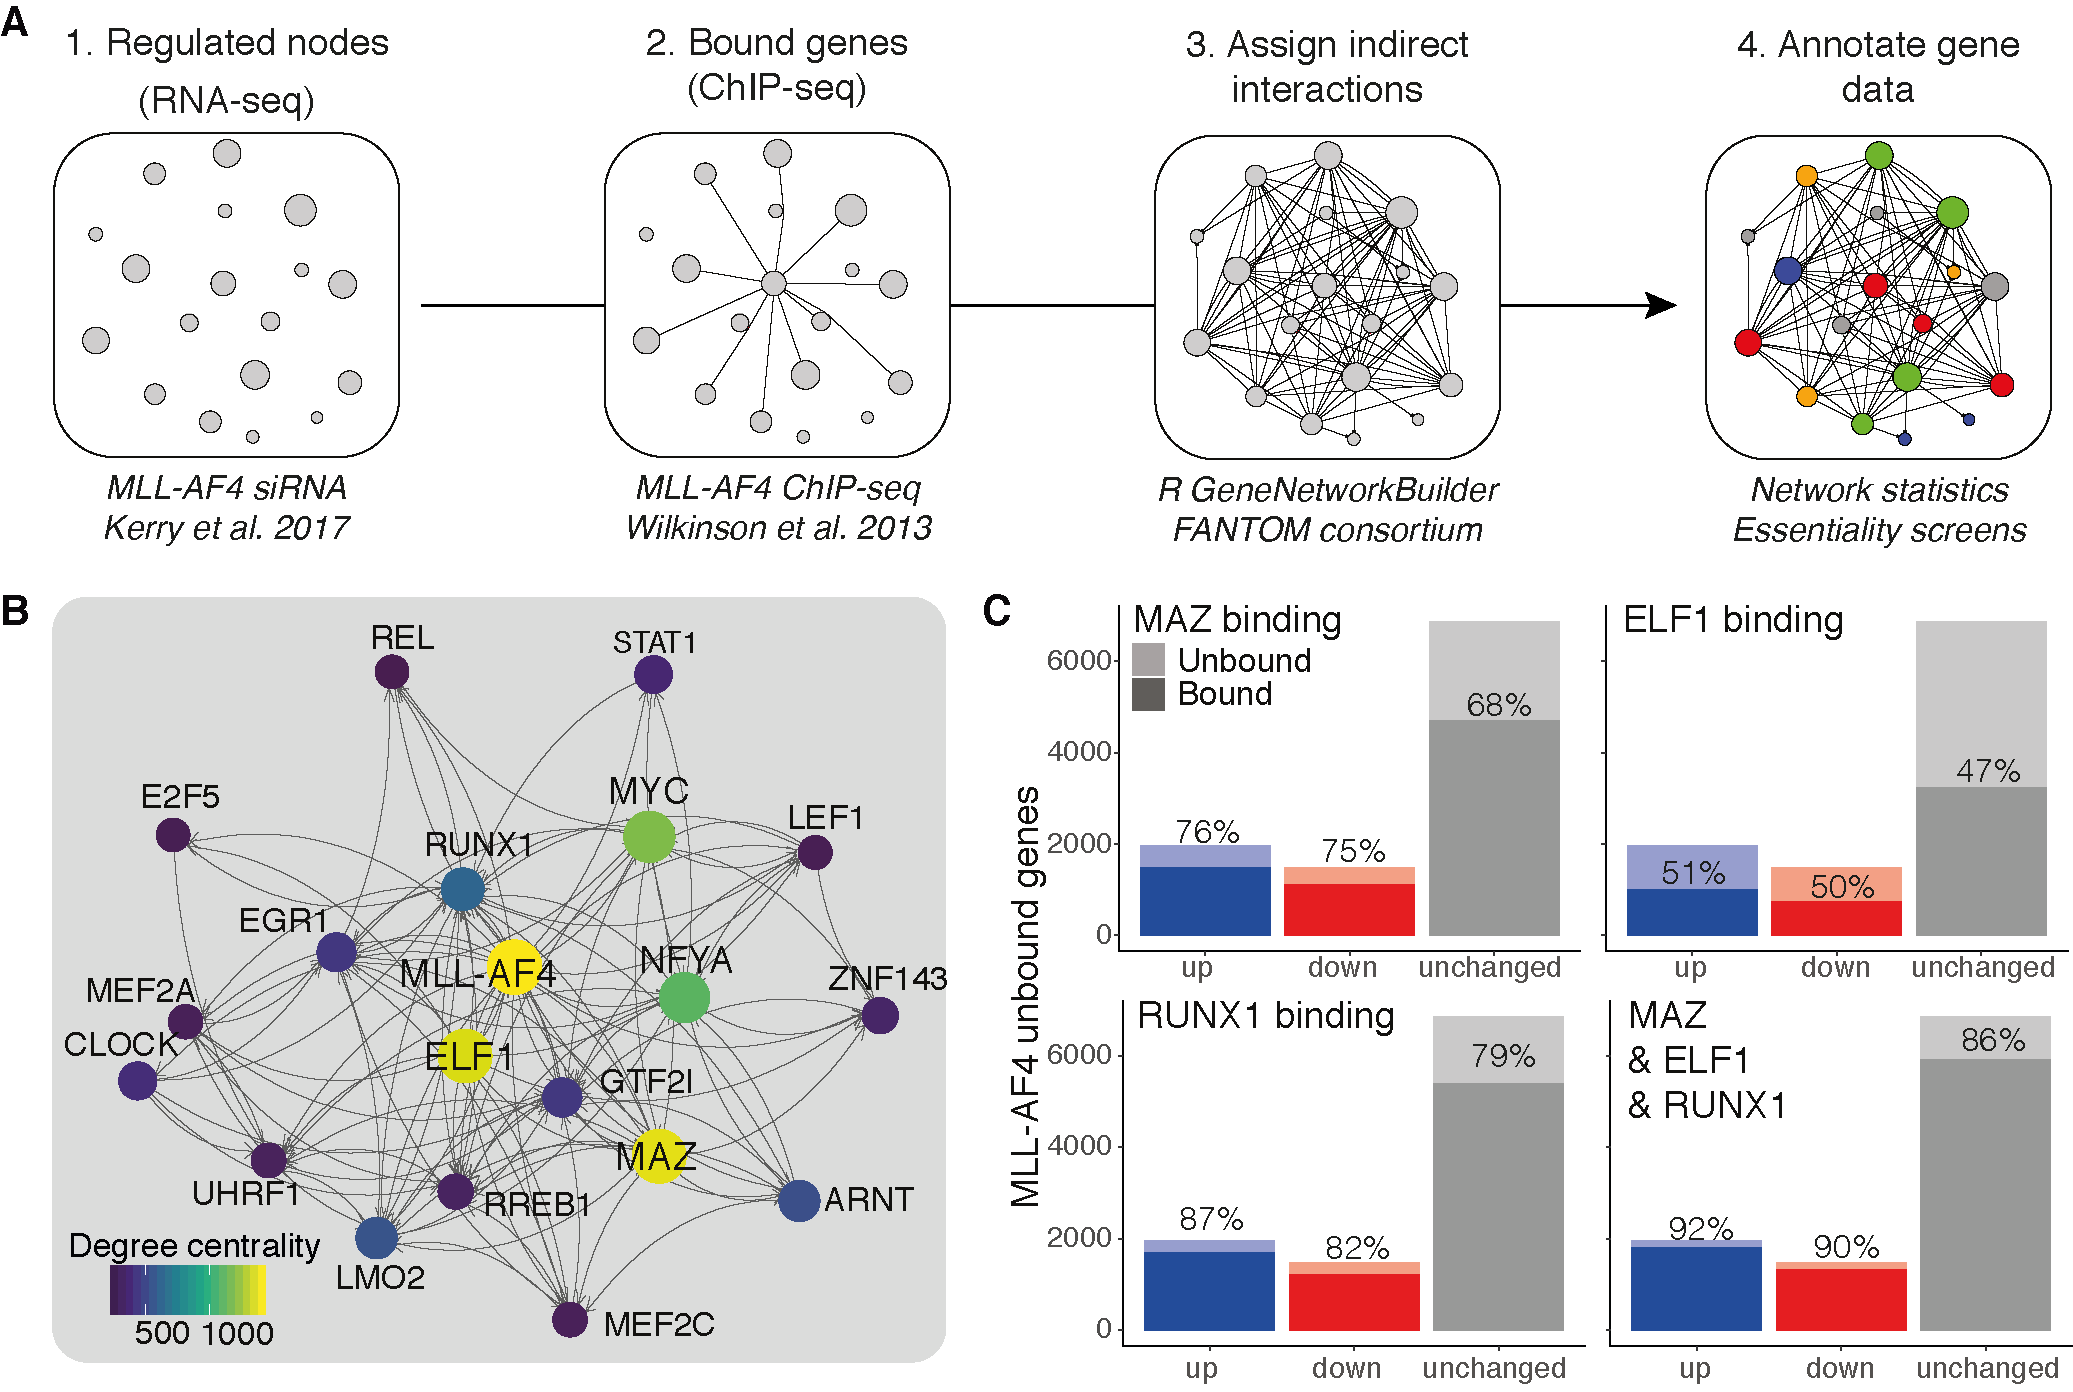
\includegraphics{figures/chapter4/ch4_ma4-grn.png}
    \caption[{Constructing an MLL-AF4 centred GRN model of MLL-AF4 leukaemia.}]
    {\textbf{Constructing an MLL-AF4 centred GRN model of MLL-AF4 leukaemia.} 
    \textbf{(A)} GRN creation workflow using siRNA KD with nascent RNA-seq, ChIP-seq, an underlying TF motif network \citep{the_fantom_consortium_and_the_riken_omics_science_center_transcriptional_2009}.
    \textbf{(B)} The top 20 genes of the MLL-AF4 GRN by degree centrality. Lines indicate predicted interaction from protein to gene locus, with arrowheads pointing downstream.
    \textbf{(C)} Number of \textit{MLL-AF4} KD DEGs that are not bound by MLL-AF4, as highlighted in Fig. \ref{fig:ch4_GRN_just}A. Shaded bars represent proportion of TF-bound DEGs. 
    \textit{Adapted from \cite{harman_kmt2a-aff1_2021}.}
    }
    \label{fig:ch4_ma4-grn}
\end{figure}

As the central hypothesis of this chapter suggests that indirectly regulated MLL-AF4 targets are affected through activated TFs, MLL-AF4 regulated TFs in the GRN must therefore bind to these indirect targets. Within the GRN a number of highly central TFs were found to be directly regulated by MLL-AF4, including ELF1, MAZ, MYC, NF-YA and RUNX1 (Fig. \ref{fig:ch4_ma4-grn}C). The Milne lab has previously shown \textit{ELF1} and \textit{RUNX1} to be MLL-AF4 targets, with a role in leukaemia \citep{godfrey_dot1l_2019, wilkinson_runx1_2013}. Interestingly, Elf1 was also identified as a central regulator for pre-HSCs in the EHT GRN (Fig. \ref{fig:ch3_centrality}, p.\pageref{fig:ch3_centrality}), suggesting that this role may be co-opted by MLL-AF4 in leukaemia. While MAZ has not previously been implicated in \textit{MLL}r leukaemias, it is known to bind and regulate \textit{MYC} \citep{komatsu_maz_1997}. MYC has a well-studied and critical role in many cancers \citep{dang_myc_2012}, supporting its place as a central TF here. NF-YA has been recently reported to have a role in \textit{MLL}r leukaemias, in that it may mediate binding of the MLL-FP complex component Menin, and subsequently the MLL-FP complex, to DNA. Inhibition of NF-YA may function synergistically with Menin-MLL1 inhibitors \citep{soto-feliciano_molecular_2022}. Taking ELF1, RUNX1 and MAZ as examples, the binding profiles of these central TFs can account for the majority of MLL-AF4 indirectly regulated targets, and their combined binding profile has the potential to regulate over 90\% of MLL-AF4 KD DEGs (Fig. \ref{fig:ch4_ma4-grn}D), highlighting the utility of this model for interrogating the wider regulatory scope of MLL-AF4.

\begin{figure}[!t]
    \centering
    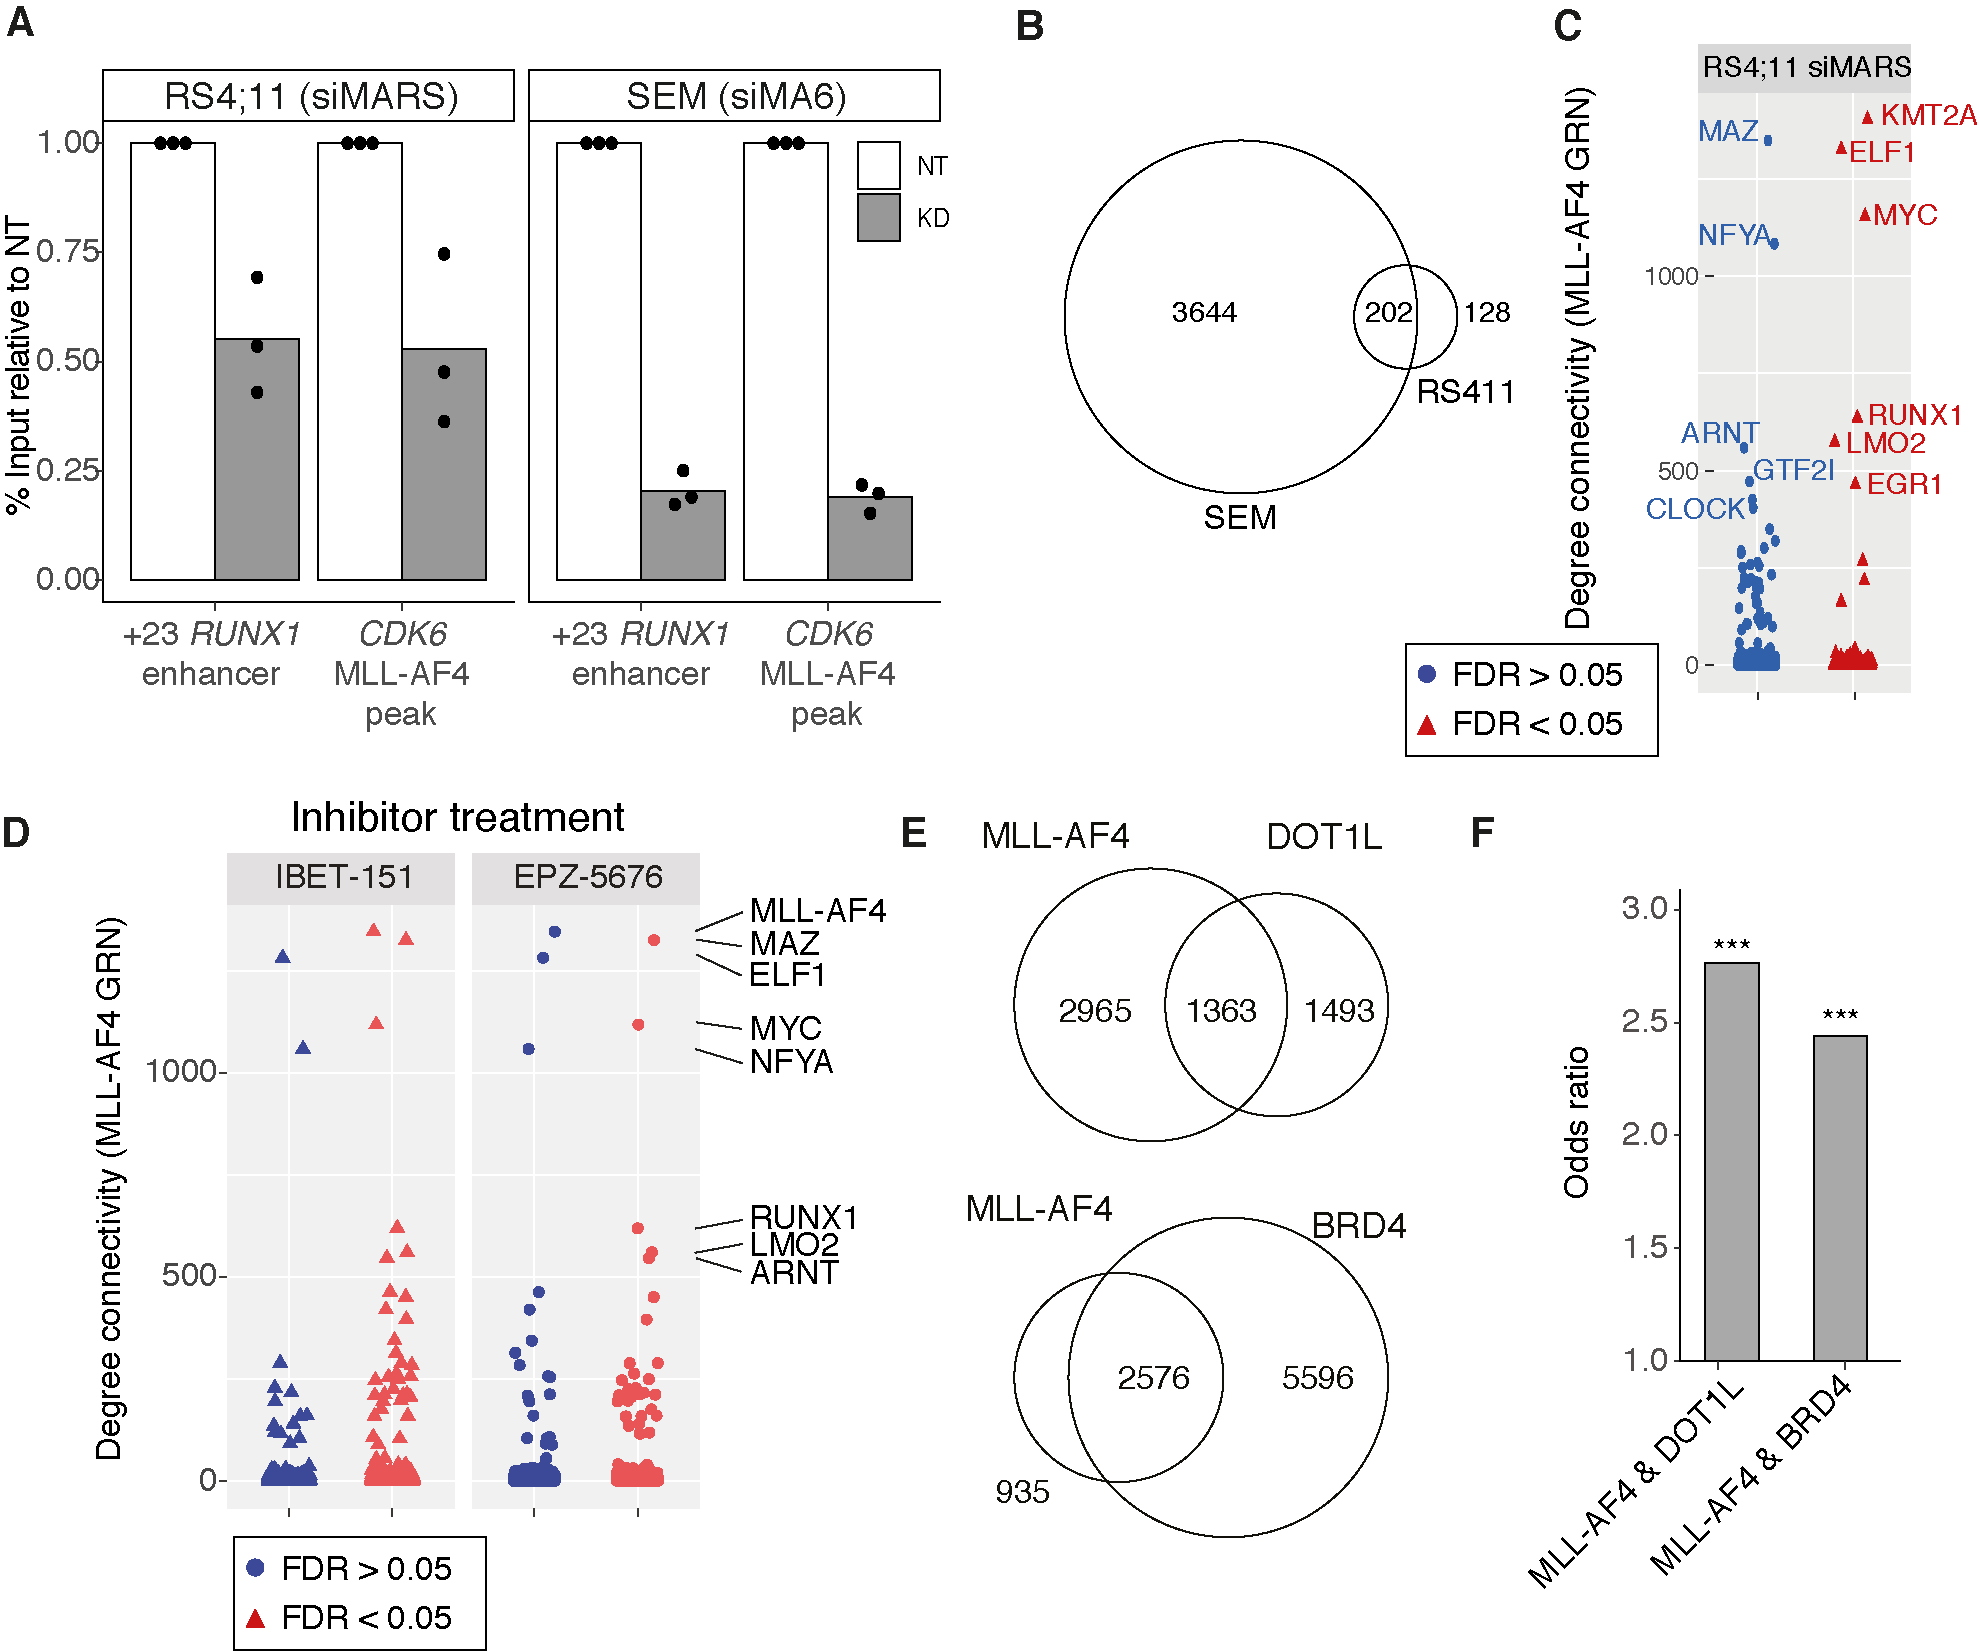
\includegraphics[width=\textwidth,height=\textheight,keepaspectratio]{figures/chapter4/ch4_grn-rs411.png}
    %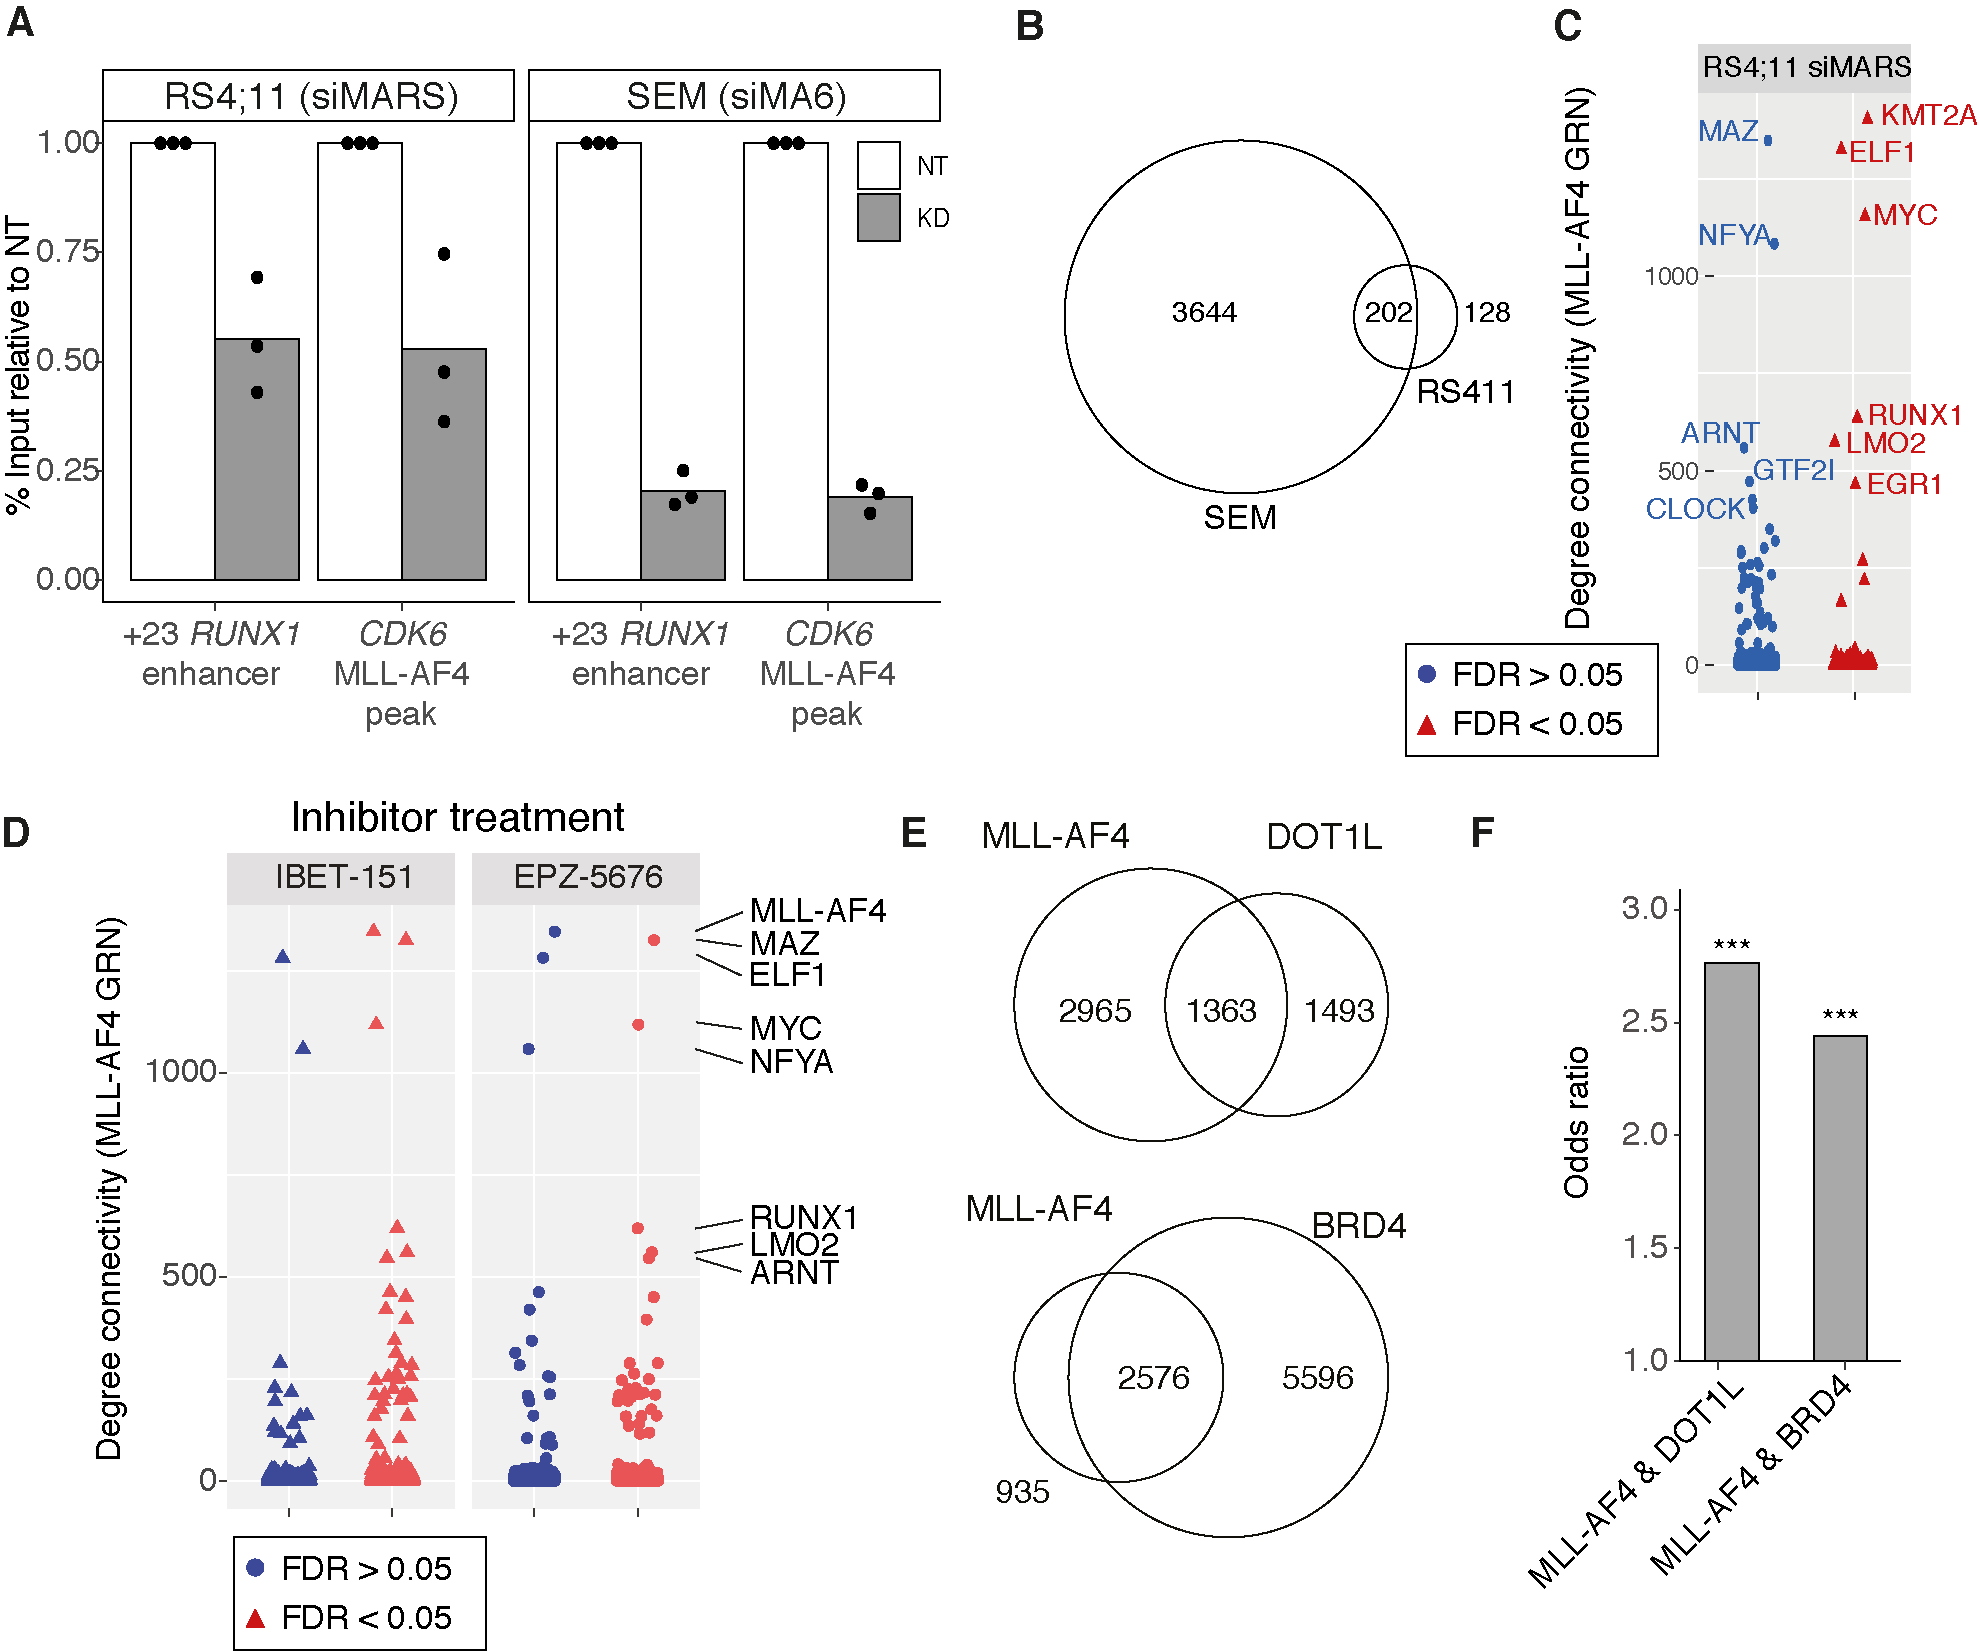
\includegraphics{figures/chapter4/ch4_grn-rs411.png}
    \caption[{Validation of the MLL-AF4 GRN.}]
    {\textbf{Validation of the MLL-AF4 GRN.} 
    \textbf{(A)} MLL-N ChIP-qPCR data in RS4;11 and SEM cells after \textit{MLL-AF4} KD, normalized to input chromatin and displayed relative to non-targeting (NT) control. siMA6 and siMARS refer to SEM and RS4;11 specific \textit{MLL-AF4} siRNA, respectively \citep{thomas_targeting_2005}. 
    \textbf{(B)} Overlap of nodes between SEM GRN and RS4;11 \textit{MLL-AF4} KD DEGs. 
    \textbf{(C-D)} Number of DEGs after \textit{MLL-AF4} KD in RS4;11 cells (\textit{n} = 3) (C), or  1.5 hours’ IBET and 7 days’ EPZ-5676 treatment (\textit{n} = 3) (D), plotted against degree centrality in the SEM MLL-AF4 GRN. Blue points: FDR > 0.05, red points: FDR < 0.05. 
    \textbf{(E)} Overlap of nodes between MLL-AF4 GRN, and IBET-151 and EPZ-5676 treatment DEGs. 
    \textbf{(F)} Fisher's exact test of overlaps shown in (E), showing odds ratios. (***) P < 0.001. 
    \textit{Raw data for D-F was generated previously in the Milne lab, and analysed by me. Adapted from \cite{harman_kmt2a-aff1_2021}.} 
    }
    \label{fig:ch4_grn-rs411}
\end{figure}

To validate this GRN model with an alternative MLL-AF4 ALL cell line, I determined how sensitive the GRN nodes are to \textit{MLL-AF4} perturbation in RS4;11 cells. I performed 96 hours' \textit{MLL-AF4} KD in both RS4;11 and SEM cells, and followed this with nascent RNA-seq. The siRNA designed for the MLL-AF4 breakpoint in RS4;11 was much less efficient than the siRNA for SEM cells, despite equivalent treatment conditions (Fig. \ref{fig:ch4_grn-rs411}A). This reduced efficacy has been observed in other studies \citep{thomas_targeting_2005, geng_integrative_2012}. Despite this reduced effectiveness of the siRNA, nascent RNA-seq analysis identified 330 DEGs, and 202 of these overlapped with the SEM MLL-AF4 GRN (Fig. \ref{fig:ch4_grn-rs411}B). Importantly, even in this reduced network many of the most central GRN nodes were still affected upon RS4;11 \textit{MLL-AF4} KD, including \textit{RUNX1}, suggesting that these central factors are highly sensitive and consistent across MLL-AF4 ALL cell lines (Fig. \ref{fig:ch4_grn-rs411}C). 

To further validate the GRN, I tested whether the GRN nodes reflect activity of MLL-AF4 complex components. DOT1L is a core complex factor \citep{bernt_mll-rearranged_2011, biswas_function_2011, lacoste_disruptor_2002, milne_leukemogenic_2005, okada_hdot1l_2005, mueller_role_2007, slany_mll_2020, lin_instructive_2016, krivtsov_h3k79_2008} that should strongly overlap with the GRN, and BRD4 is an associated cofactor with a general role in gene activation \citep{dawson_inhibition_2011, zuber_rnai_2011} that is not specific to the MLL-AF4 complex. Comparing the MLL-AF4 GRN with DEGs following 7 days’ EPZ-5676 (DOT1L inhibitor) treatment and 1.5 hours’ IBET-151 (BRD4 inhibitor) treatment (Published data from \cite{godfrey_dot1l_2019} and \cite{crump_bet_2021}), both inhibitors overlapped with the GRN and impacted central TFs (Fig. \ref{fig:ch4_grn-rs411}D-E). DOT1L inhibition impacted less of the MLL-AF4 GRN than BRD4, but with greater specificity (Fig. \ref{fig:ch4_grn-rs411}F). This analysis serves to validate that the MLL-AF4 GRN represents aspects of BRD4 and DOT1L activity and is therefore a reliable representation of MLL-AF4 complex behaviour.

\section[Integrating patient expression data highlights regulatory modules, and a set of “core” MLL-FP TFs]{\label{ch4:patient}Integrating patient expression data highlights regulatory modules, and a set of “core”\\MLL-FP TFs}

\begin{figure}[!t]
    \centering
    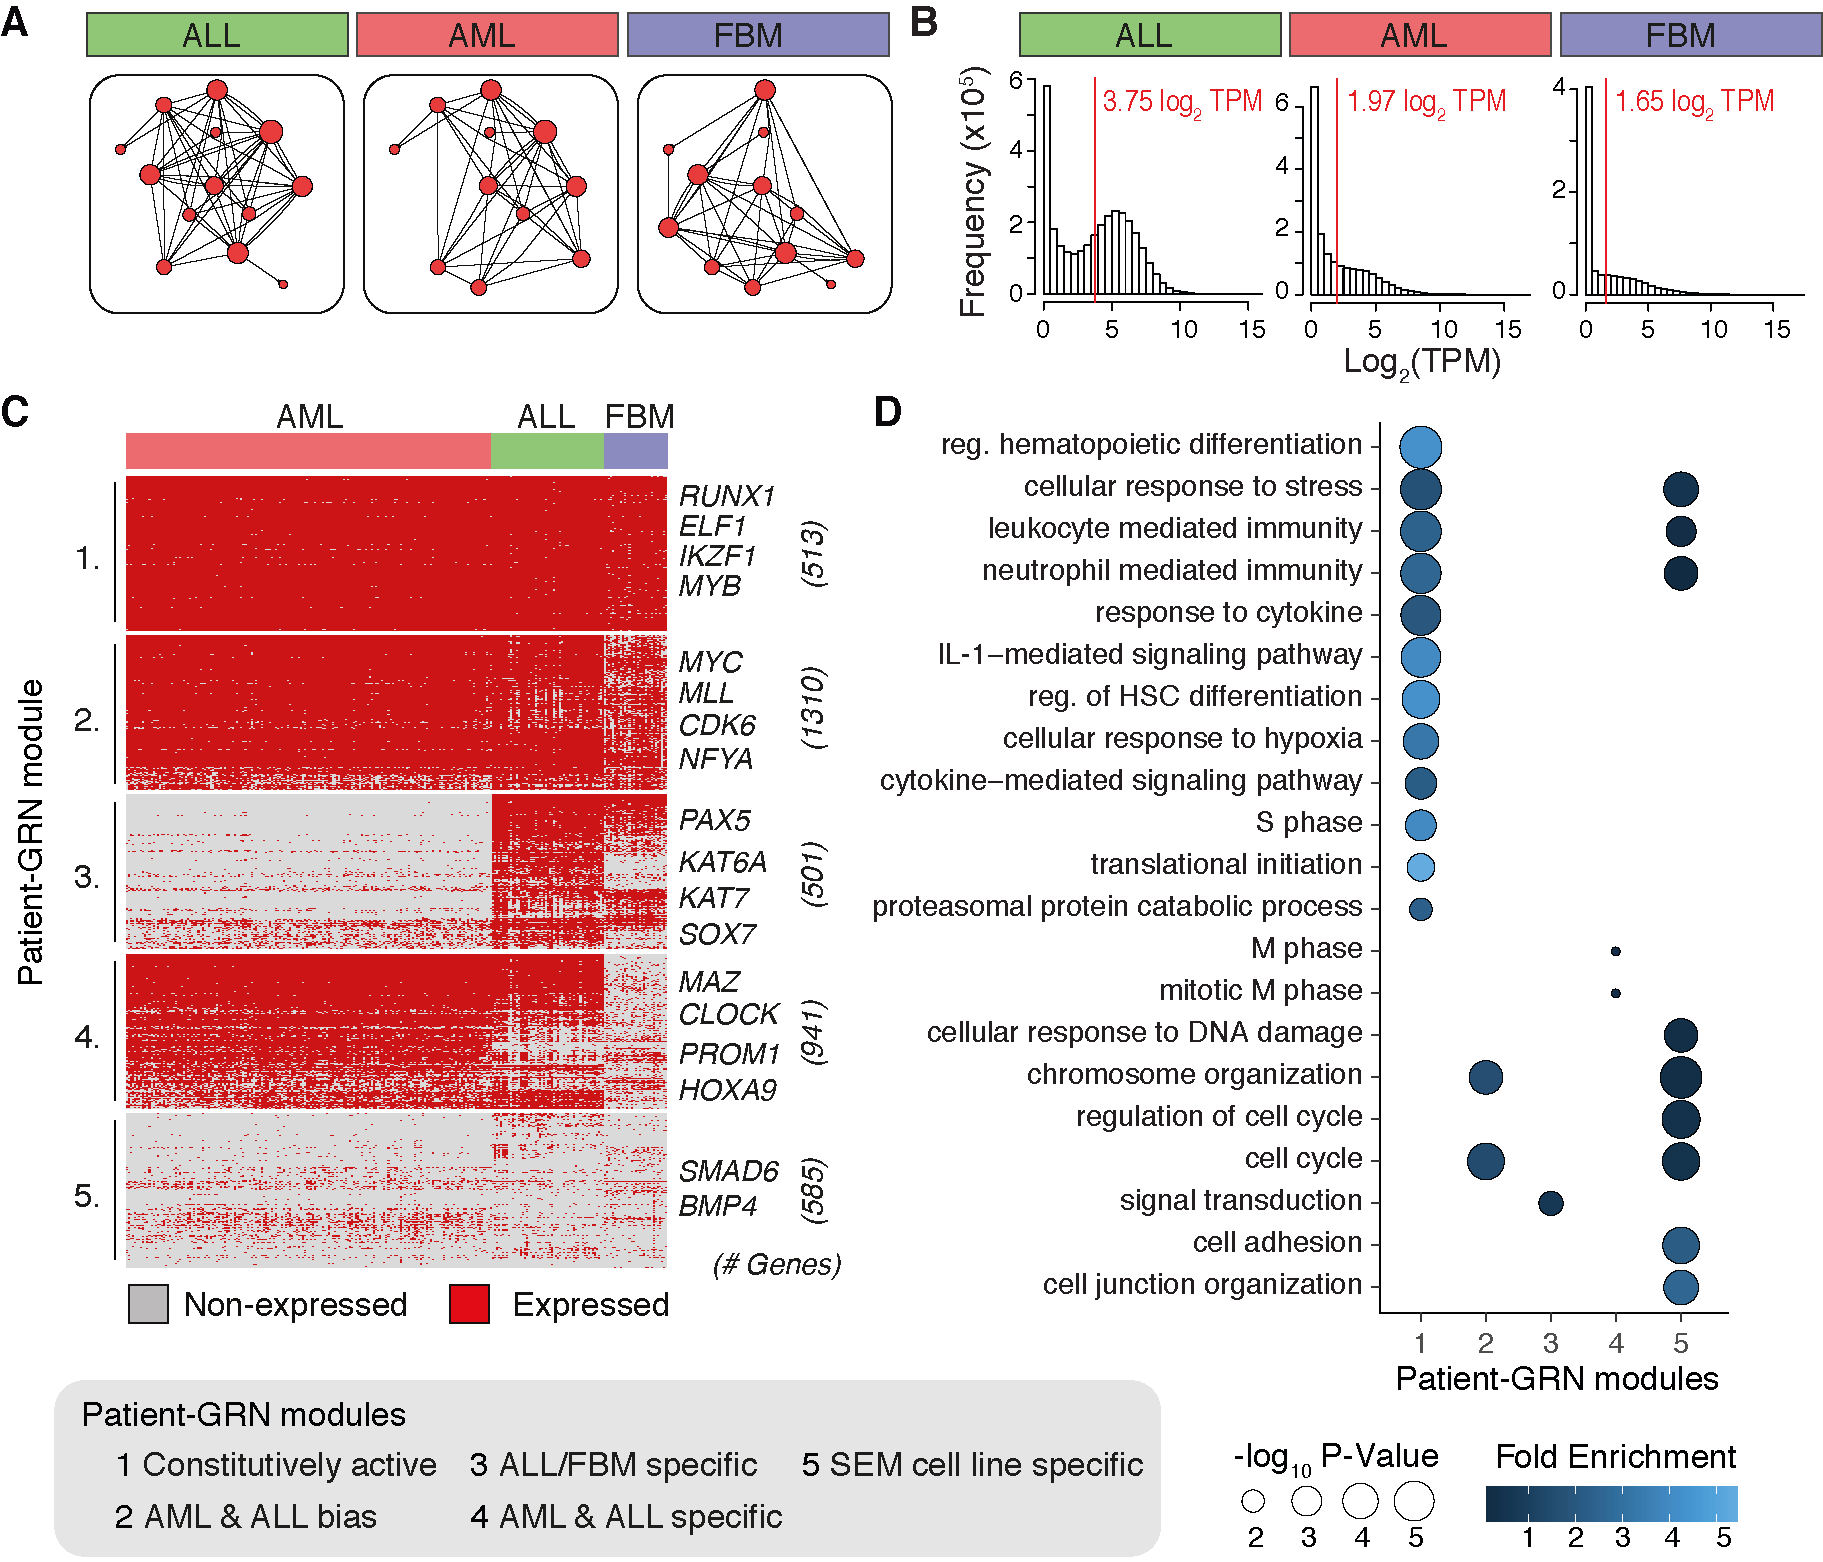
\includegraphics[width=\textwidth,height=\textheight,keepaspectratio]{figures/chapter4/ch4_patient.png}
    %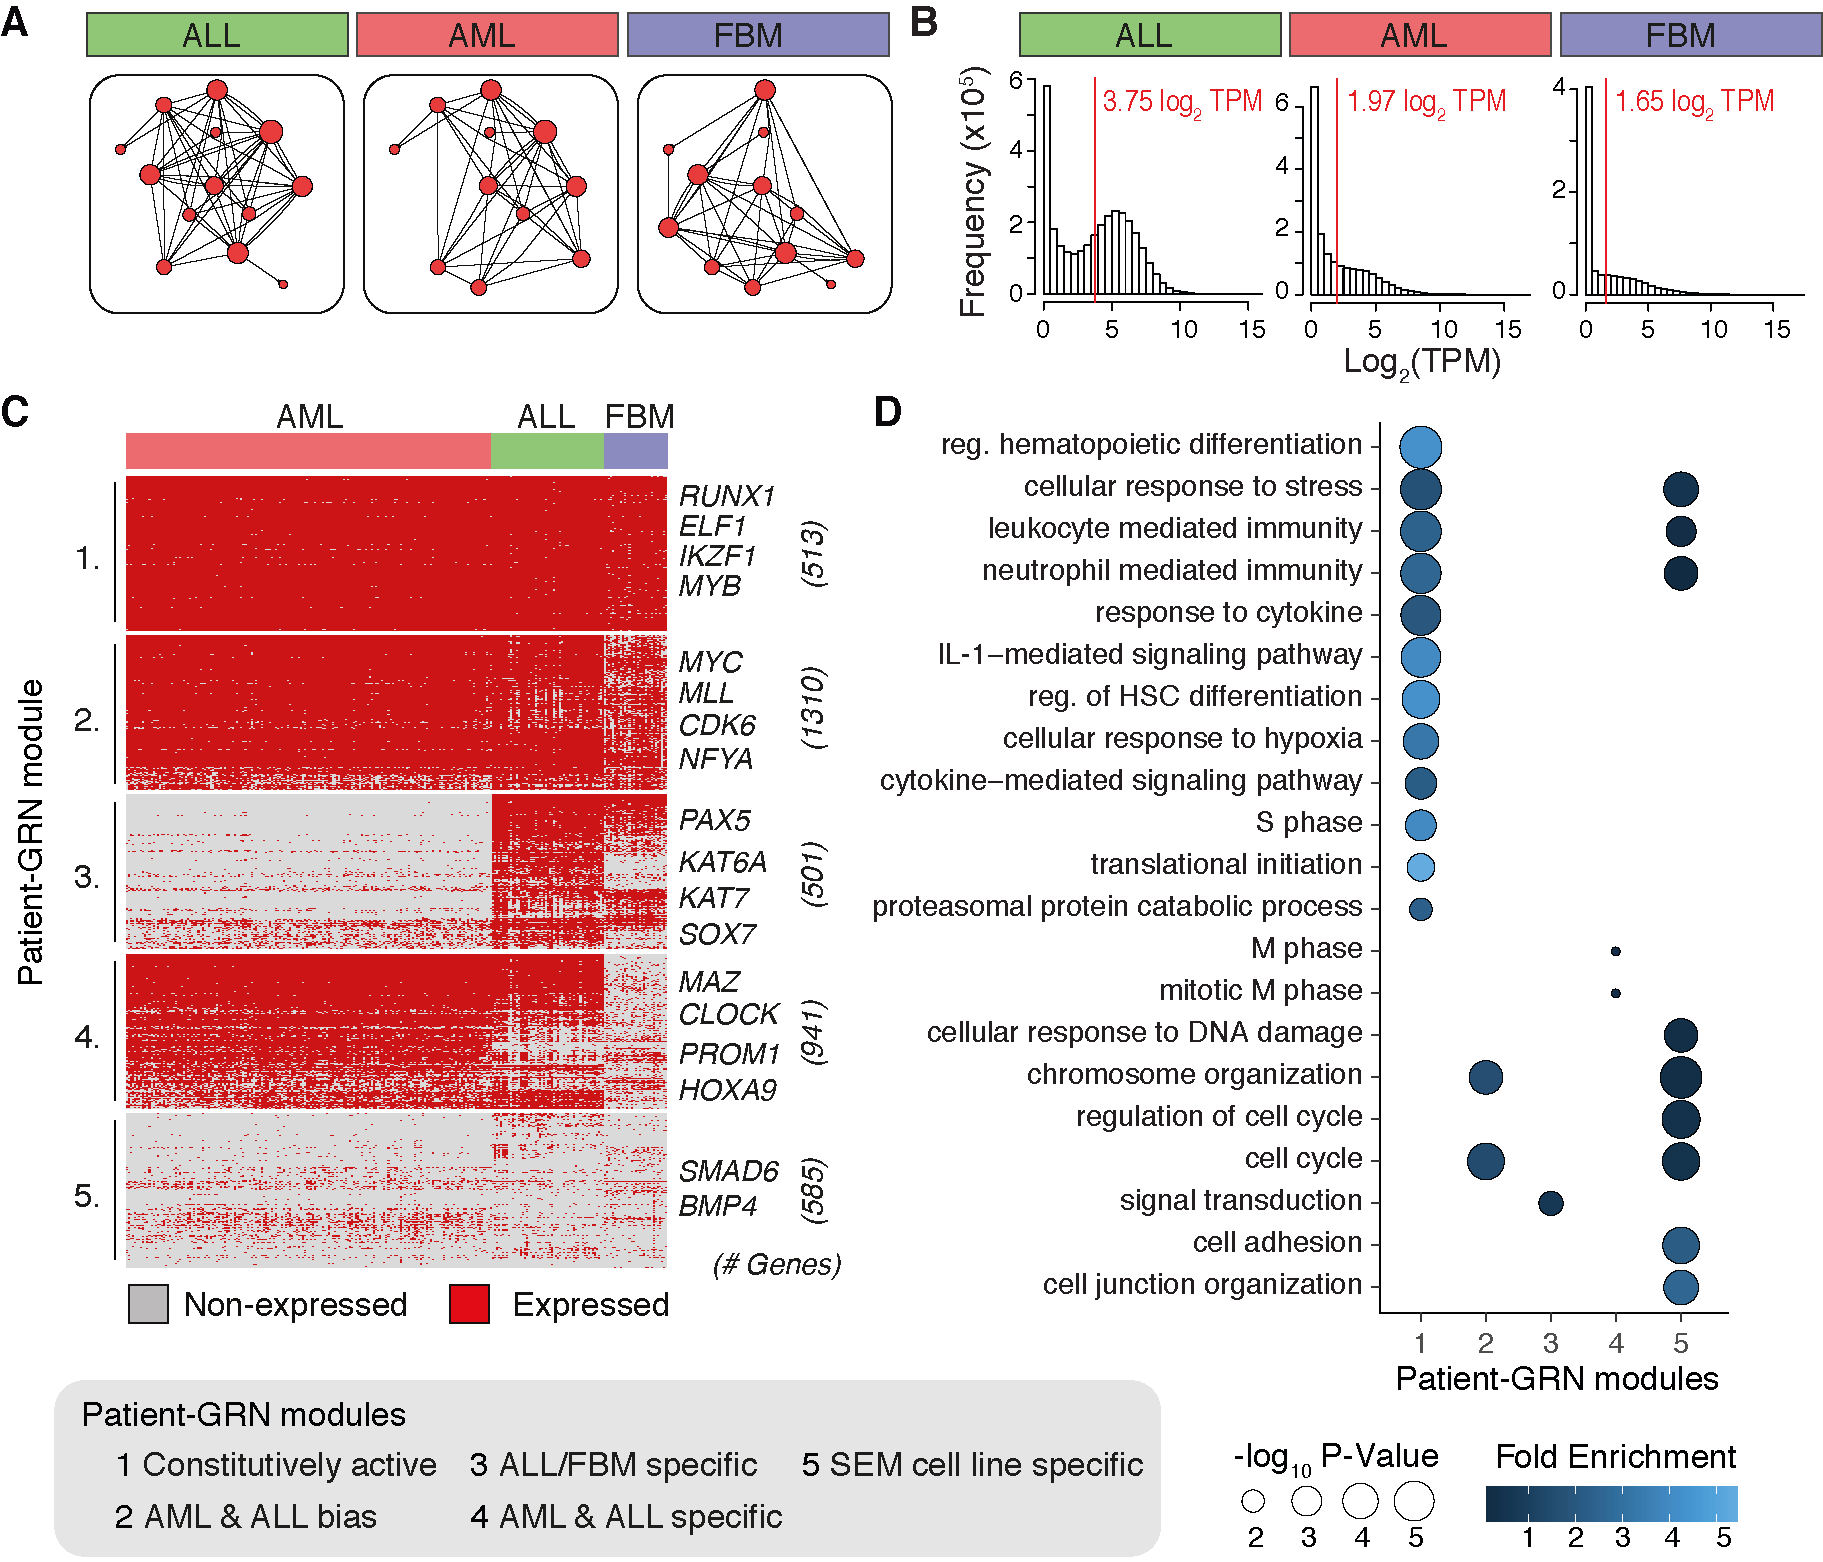
\includegraphics{figures/chapter4/ch4_patient.png}
    \caption[{The MLL-AF4 GRN can be split into regulatory modules based on patient gene expression.}]
    {\textbf{The MLL-AF4 GRN can be split into regulatory modules based on patient gene expression.} 
    \textbf{(A)} Schematic illustration of sub-networks reflecting expressed genes in patient samples. 
    \textbf{(B)} Histograms of log\textsubscript{2} TPM expression in AML, ALL and FBM datasets. Red line indicates threshold for defining active gene expression (mean log\textsubscript{2} TPM). 
    \textbf{(C)} GRN node activity across sub-networks as defined in B. Genes were grouped into patient-GRN modules using \textit{k}-means. Rows represent genes; columns represent samples. 
    \textbf{(D)} GO biological process enrichment for patient-GRN modules. 
    \textit{Normalised expression data for this analysis was sourced from published data, with GRN analyses performed by me. Adapted from \cite{harman_kmt2a-aff1_2021}.}
    }
    \label{fig:ch4_patient}
\end{figure}

\textit{MLL} translocations can involve many different fusion partners, and can result in either ALL or AML. There are also cases where lineage switching occurs after relapse \citep{dorantes-acosta_lineage_2012, gardner_acquisition_2016}. This suggests similarity in the behaviour across different MLL-FP complexes, in both ALL and AML lineages, and suggests there may be a core set of targets driven by MLL-FPs more generally. Further, the translocation events often occur in utero resulting in infant and childhood leukaemias \citep{greaves_causal_2018, greaves_utero_2005, ford_utero_1993, jackson_origin_2021}, and fetal programs can be overexpressed in \textit{MLL}r leukaemia \citep{rice_human_2021}, indicating that the MLL-AF4 GRN originates in a fetal regulatory landscape. To assess whether the GRN model represents common ALL and AML biology, or shares characteristics with fetal B-cell development, I overlapped the GRN with patient and fetal bone marrow (FBM) expression data to create sub-networks (Fig. \ref{fig:ch4_patient}A). Expression data was taken from \textit{MLL}r ALL patients \citep{agraz-doblas_unraveling_2019}, AML patients with various chromosomal abnormalities \citep{the_cancer_genome_atlas_research_network_genomic_2013}, and HSPCs and B cells from normal FBM \citep{obyrne_discovery_2019}. These FBM populations included HSCs, multipotent progenitors (MPP), lympho-myelo primed progenitors (LMPP), pre-pro-B and pro-B cells. A threshold was used to define active genes, based on the mean gene expression within each dataset. Active genes were used to filter the MLL-AF4 GRN into patient specific sub-networks (Fig. \ref{fig:ch4_patient}B, methods section \ref{ch2:ma4-grn}, p.\pageref{ch2:ma4-grn}). Median expression was unusable due to low sequencing depth in the FBM data.

\subsection{\label{ch4:patient-modules}Regulatory modules of the GRN}

A binary matrix of gene activity across sub-networks was generated, then clustered into five patient-GRN modules (Fig. \ref{fig:ch4_patient}C). Note that \textit{MLL} expression in the case of \textit{MLL}r leukaemias also includes MLL-FP activity. A caveat of this analysis is that levels of expression are not addressed, which may have more subtle but important consequences. For example, \textit{RUNX1} is present in module 1 and active across all samples, however \textit{RUNX1} has been shown to be overexpressed in MLL-AF4 ALLs compared to MLL-AF9 AML and is important for leukaemic growth \citep{wilkinson_runx1_2013}. Thus, expression level rather than simply just presence of gene expression is likely an important indicator of functional importance. Nevertheless, this analysis serves to highlight modules that are potentially important across multiple leukaemias. 

Nodes in modules 1 and 2 are active across all leukaemias and FBM populations and are associated with haematopoietic differentiation as a key process, emphasising a maintained fetal haematopoietic program (Fig. \ref{fig:ch4_patient}D). Module 3 is active in ALL and a subset of FBM samples, and identifies \textit{SOX7} and \textit{KAT6A} as ALL-specific, and \textit{PAX5} and \textit{KAT7} in both ALL and FBM (Fig. \ref{fig:ch4_patient}C). The lack of AML activity implies this module differentiates ALL and AML, reinforced by the presence of \textit{PAX5}, a critical regulator of B lymphopoiesis \citep{medvedovic_pax5_2011}, and \textit{SOX7}, which is highly expressed in ALL over AML and drives proliferation \citep{cuvertino_sox7_2016}. Module 4 is instead active in both AML and ALL datasets, with low activity in FBM samples (Fig. \ref{fig:ch4_patient}C), indicating nodes distinct from the normal B progenitor program. Interestingly, this includes the central GRN node \textit{MAZ}, indicating it is a leukaemia specific target. \textit{PROM1} (CD133) is also in this cluster, which is normally expressed in more stem and progenitor cells but can be dramatically upregulated by MLL-FPs and is essential for many ALL leukaemias \citep{godfrey_h3k79me23_2021, mak_mixed_2012, obyrne_discovery_2019}. Module 5 is inactive across all datasets (Fig. \ref{fig:ch4_patient}C), and pathway enrichment shows terms related to cell junction organisation and adhesion, response to stress, and DNA damage response (Fig. \ref{fig:ch4_patient}D), which likely represents an immortalised cell program. Together, this analysis breaks down the MLL-AF4 GRN into different modules representing ALL specific, core AML and ALL, and B-lymphopoiesis co-opted circuits. ALL specific nodes are expected as an ALL based GRN, while nodes active in both ALL and FBM populations are suggestive of a B progenitor program maintained in ALL, which may be overactivated by MLL-AF4. A particularly interesting subset are nodes active in both ALL and AML. This is indicative of a program active in both lineages, and as \textit{MLL}r may undergo lineage switching, this may represent a consistent program that enables this switch to occur.

\subsection{\label{ch4:patient-core}High centrality nodes represent a core MLL-FP program}

As MLL-AF4 may regulate a core set of nodes across lineages (Fig. \ref{fig:ch4_patient}C), it is important to establish which TFs drive this core program. The most central nodes of the SEM MLL-AF4 GRN (degree centrality > 500) are active across all ALL and AML patient sub-networks (Fig. \ref{fig:ch4_core}A), suggesting these TFs play a common role across lineages. Central GRN nodes are considerably less conserved in the fetal B progenitor program (Fig. \ref{fig:ch4_core}A), suggesting that this is regulated by distinct TFs, although this could be a consequence of the low sequencing depth or diversity of fetal populations. Patient-GRN modules 1, 2 and 4 represent the core regulatory logic between acute leukaemias (Fig. \ref{fig:ch4_patient}C), and show strikingly higher centrality compared to modules 3 and 5 (Fig. \ref{fig:ch4_core}B). Therefore, the central factors of these clusters can be taken as a panel of core TFs applicable to both AML and ALL (Fig. \ref{fig:ch4_core}C).

\begin{figure}[!t]
    \centering
    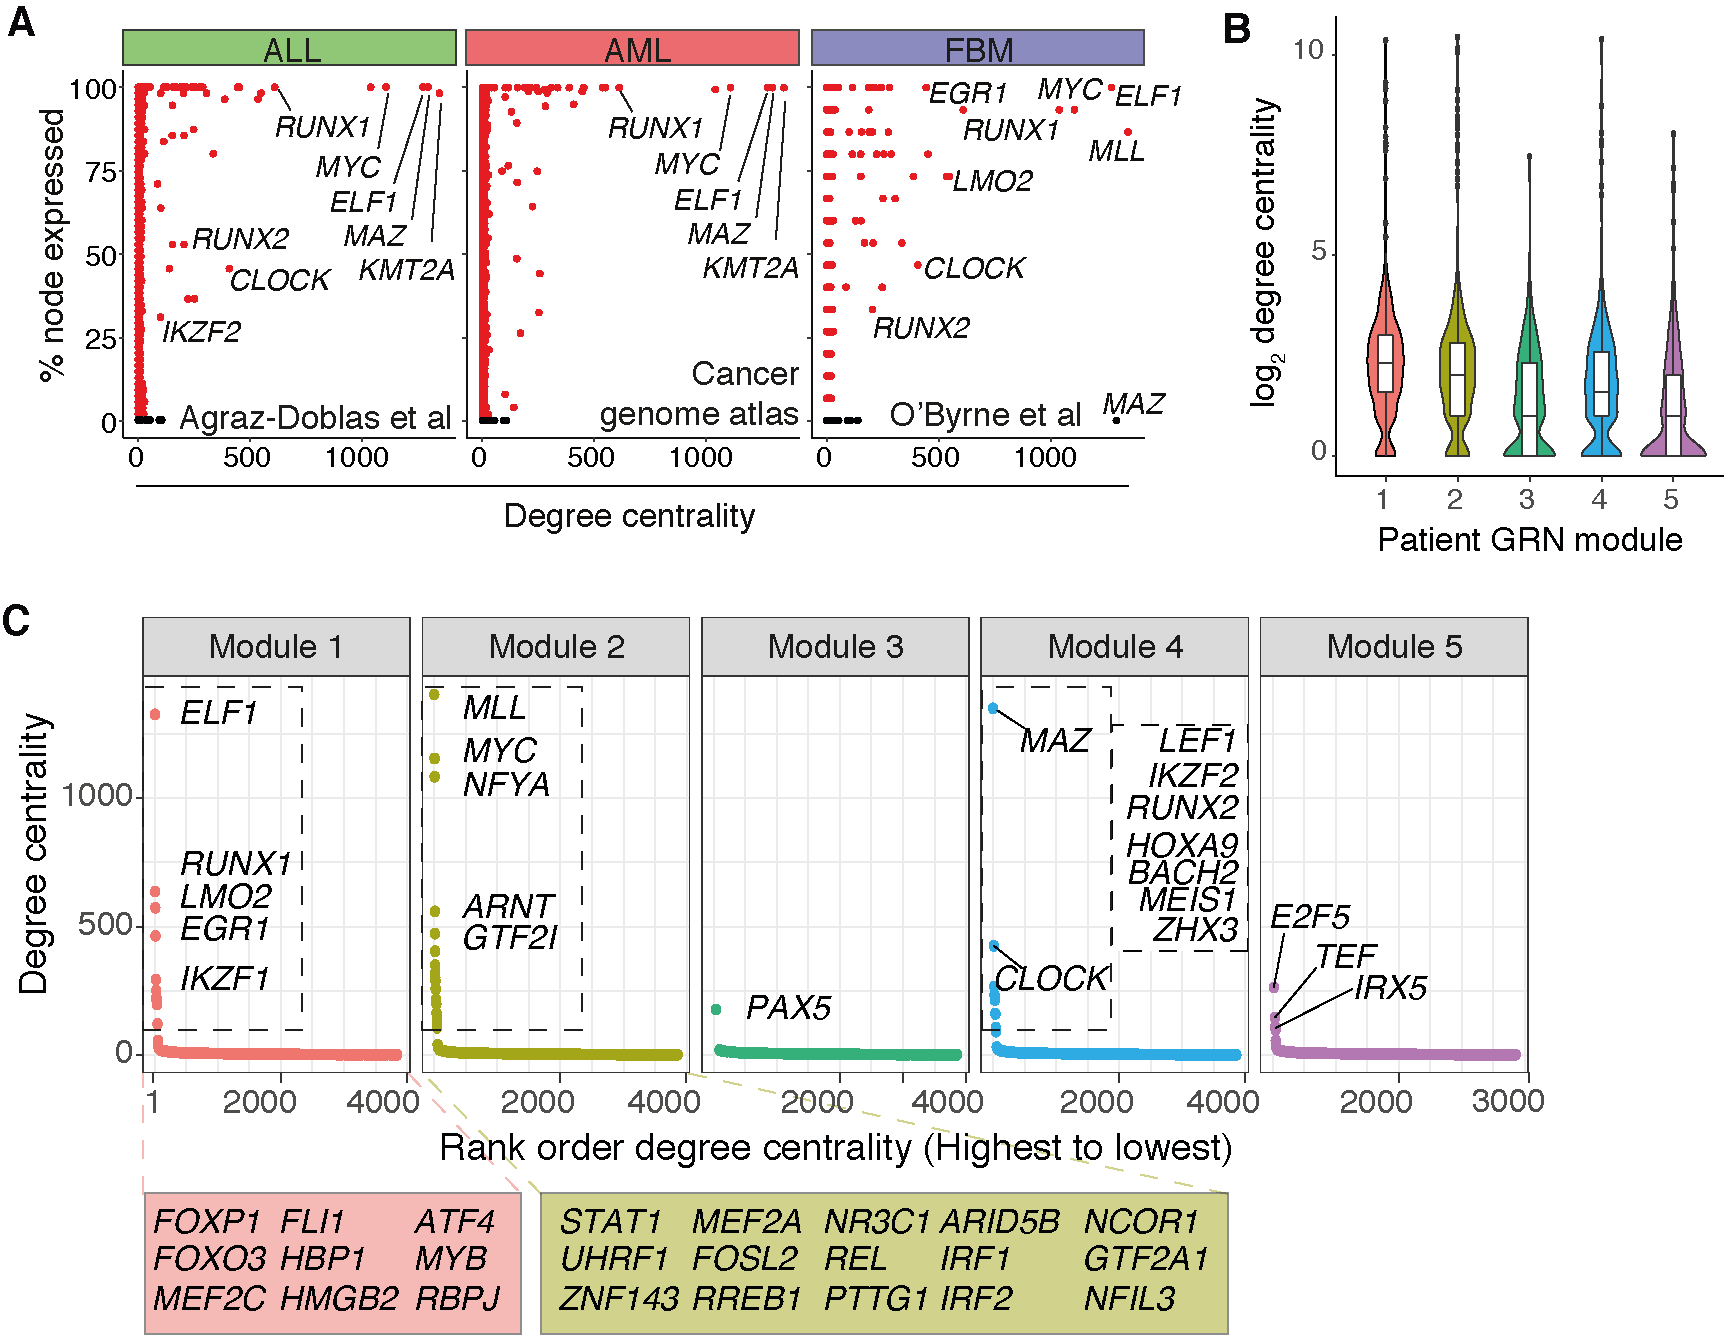
\includegraphics[width=\textwidth,height=\textheight,keepaspectratio]{figures/chapter4/ch4_core-nodes.png}
    %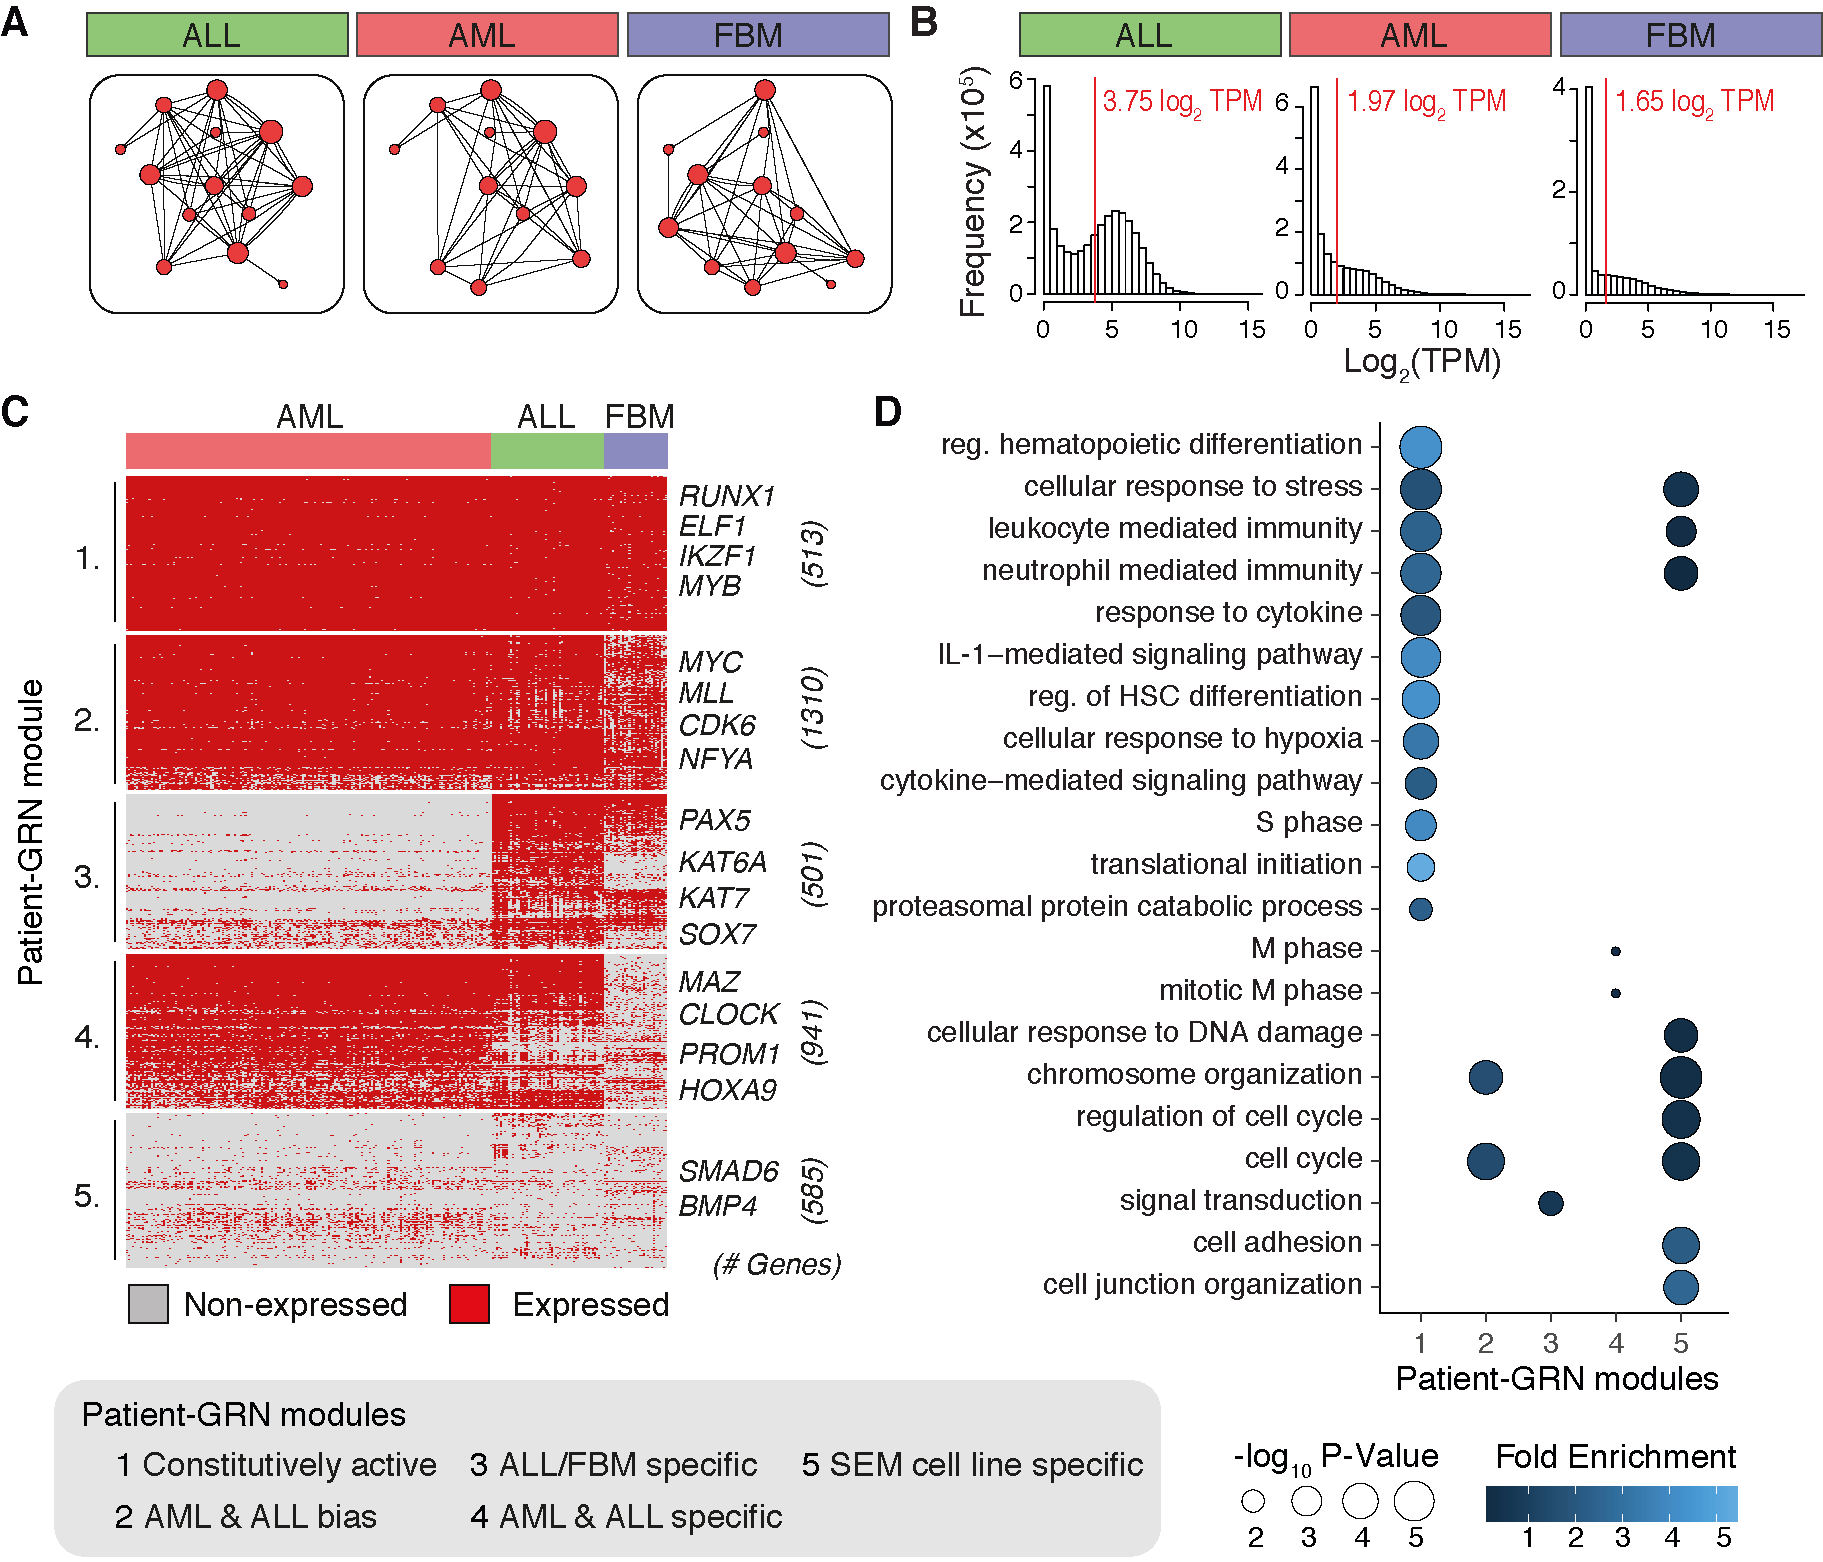
\includegraphics{figures/chapter4/ch4_patient.png}
    \caption[{Patient expression modules reveal a set of core, central nodes.}]
    {\textbf{Patient expression modules reveal a set of core, central nodes.} 
    \textbf{(A)} Relationship between percentage of patient samples expressing each gene and MLL-AF4 GRN centrality. 
    \textbf{(B)} Distribution of log\textsubscript{2} degree centrality of GRN nodes, stratified by patient-GRN module.  
    \textbf{(C)} Top-most GRN nodes by degree centrality, stratified by patient-GRN modules. Annotated nodes in Clusters 1, 2, and 4 represent the core TFs of the GRN model. 
    \textit{Adapted from \cite{harman_kmt2a-aff1_2021}.}
    }
    \label{fig:ch4_core}
\end{figure}

The analysis so far has identified highly connected TFs present across AML and ALL lineages. This has focused on the MLL-AF4 centred GRN, but our analysis could be extended to other MLL-FPs, such as MLL-AF9, to determine if there is a general MLL-FP core network. To test this, I compared MLL-N ChIP-seq profiles between SEM and THP-1 cells (MLL-AF9 AML). Of SEM MLL-AF4 bound genes in the MLL-AF4 GRN, 66\% are bound by MLL-AF9 in THP-1 cells (Fig. \ref{fig:ch4_sem-thp1}A). To determine whether this commonality extends to central targets of MLL-AF4, I performed the same comparison with RUNX1 ChIP-seq. Interestingly, only 35\% of SEM RUNX1 bound genes are in common with THP-1, suggesting that while there is common MLL-FP behaviour the central TFs are lineage specific (Fig. \ref{fig:ch4_sem-thp1}A). MLL-AF4 and MLL-AF9 binding profiles are broadly similar at common gene targets (Fig. \ref{fig:ch4_sem-thp1}B), with similar enhancer occupancy and MLL-FP spreading \citep{kerry_mll-af4_2017}. The core TF program is largely bound by MLL-FP in both SEM and THP-1 cells, with some exceptions including \textit{MAZ}, \textit{NFYA} and \textit{EGR1} (Fig. \ref{fig:ch4_sem-thp1}D). In contrast, RUNX1 binding profiles at enhancers differ, such as at the \textit{GFI1} locus (Fig. \ref{fig:ch4_sem-thp1}C). Despite these differences, many of the central GRN factors are bound by RUNX1 in both cell types (Fig. \ref{fig:ch4_sem-thp1}E). These analyses validate the capacity of the core MLL-FP TFs to regulate both ALL and AML leukaemias, using different MLL fusion partners, and highlight differences in RUNX1 binding between lineages. The core program of these leukaemias are similar, but the wider regulatory network may be context dependent.

\begin{figure}[htbp]
    \centering
    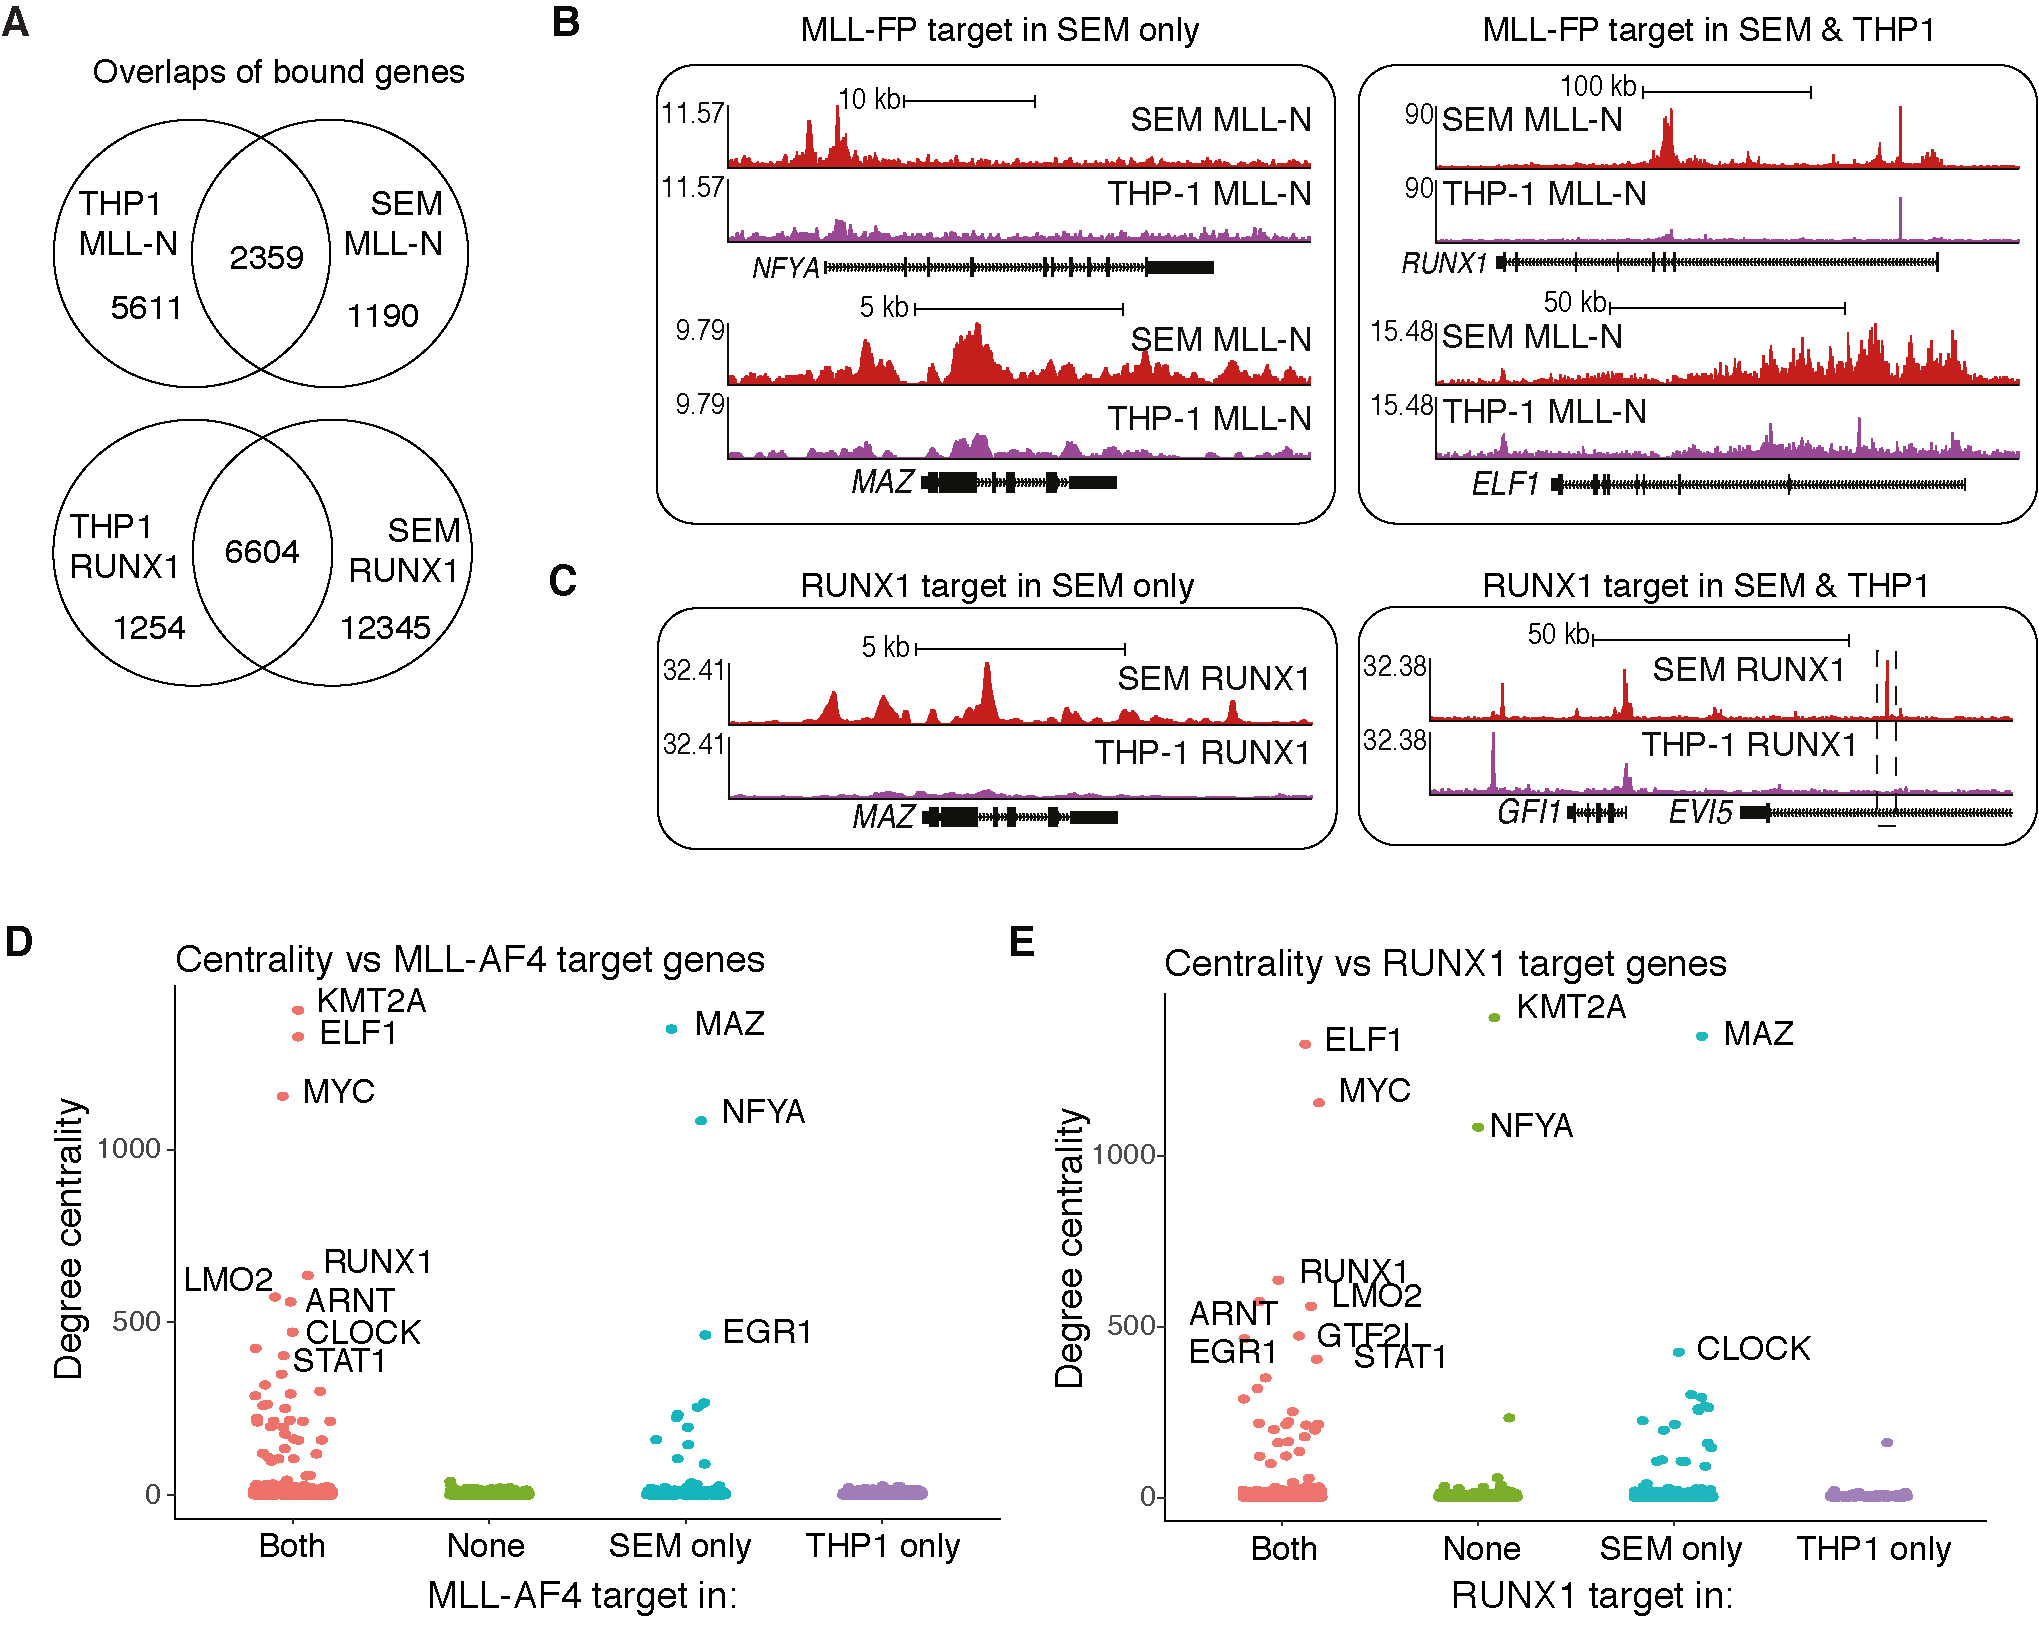
\includegraphics[width=\textwidth,height=\textheight,keepaspectratio]{figures/chapter4/ch4_sem-thp1.png}
    %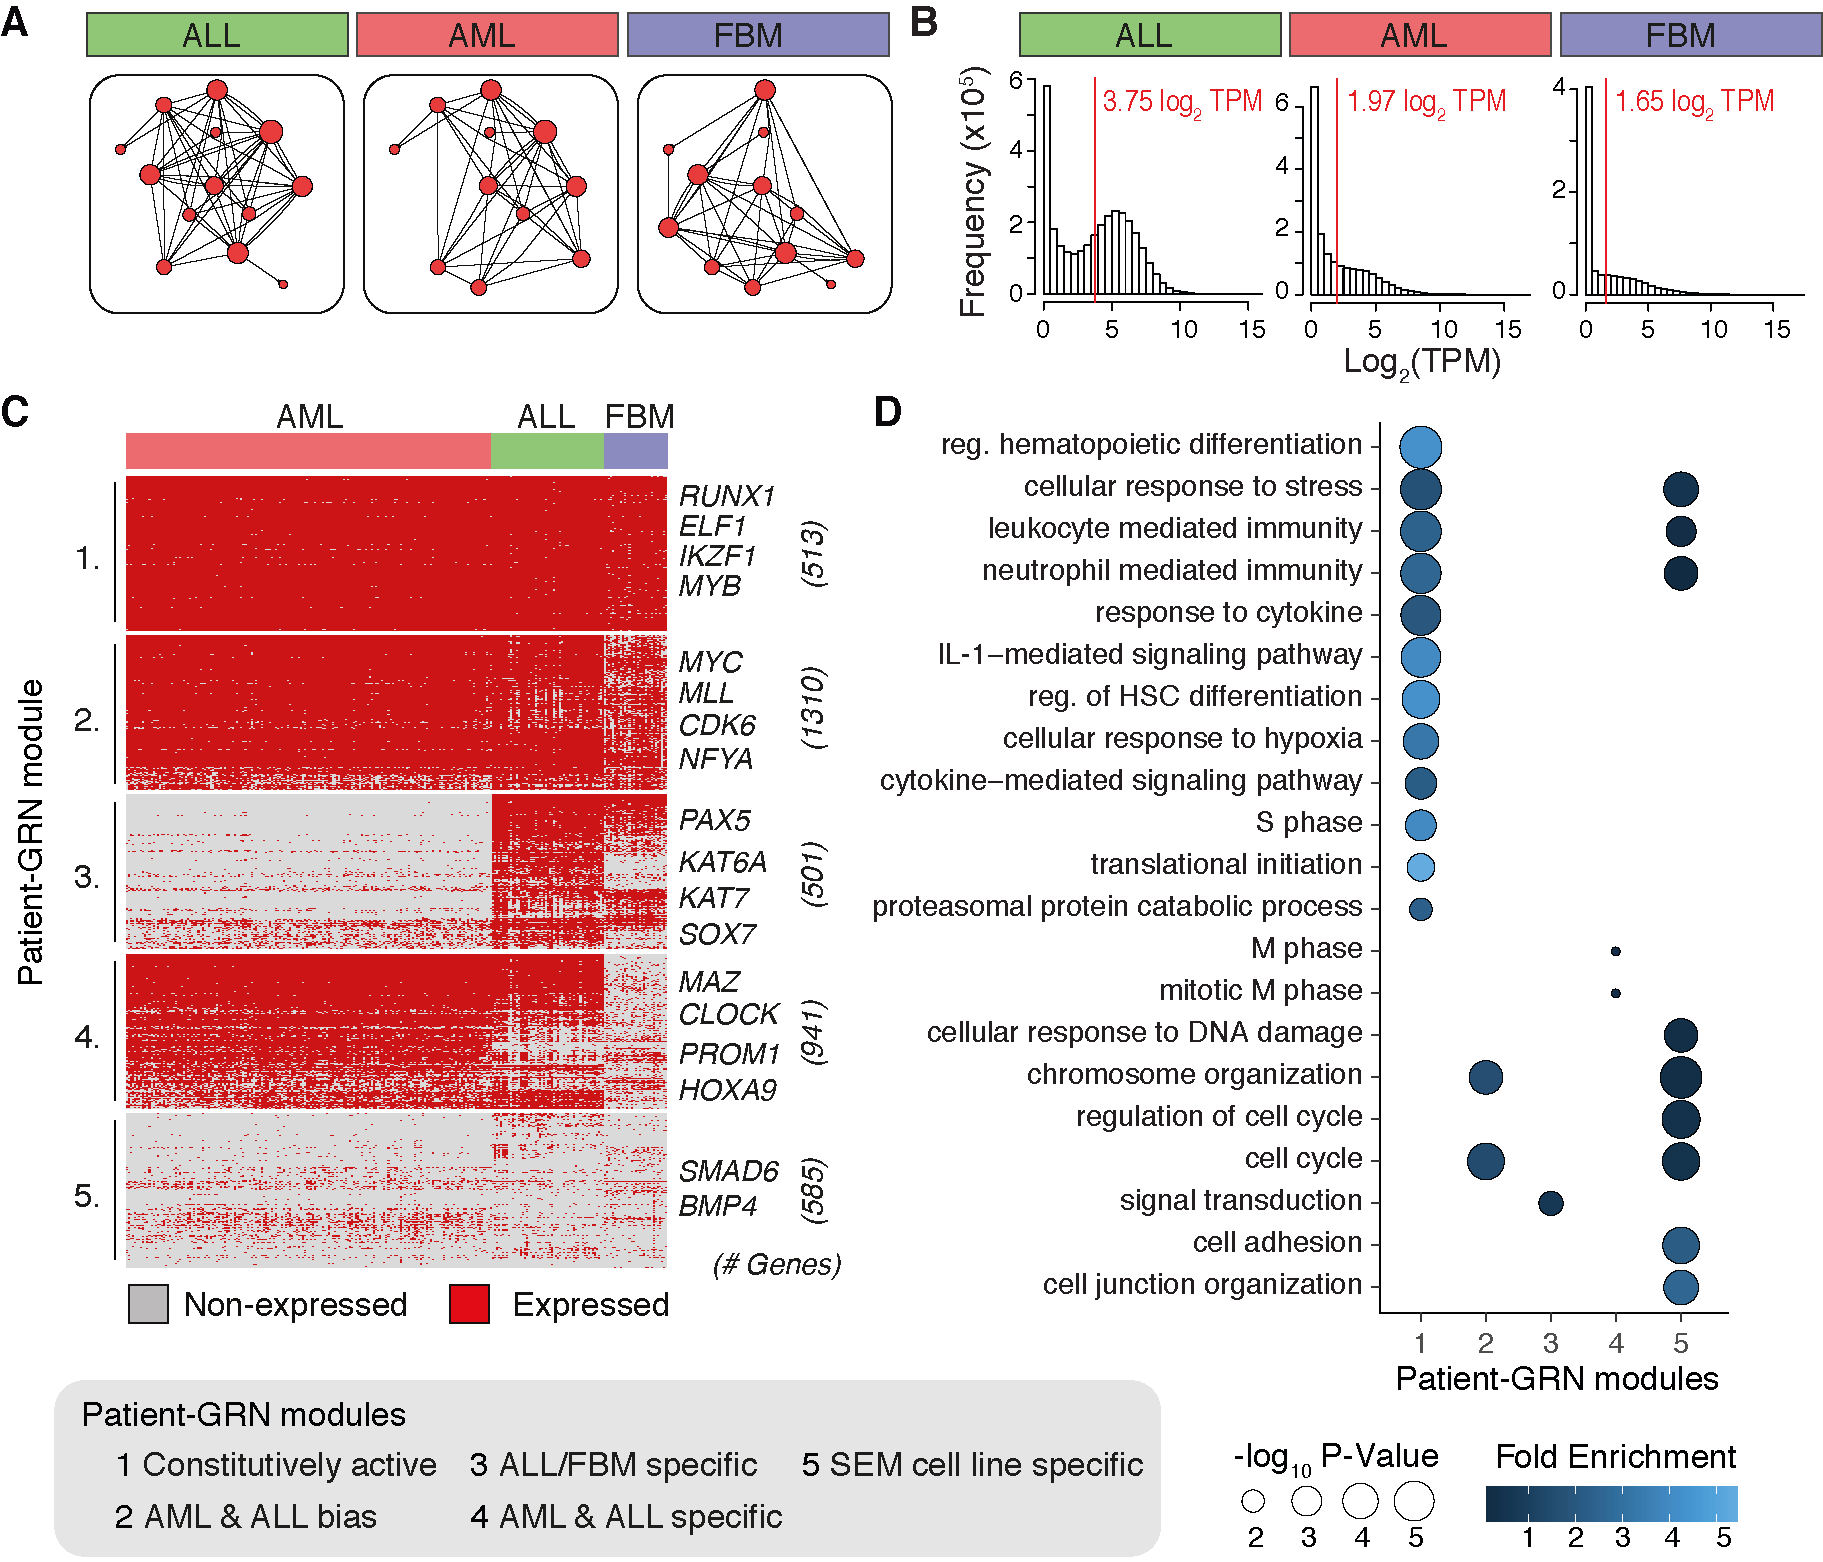
\includegraphics{figures/chapter4/ch4_patient.png}
    \caption[{The MLL-AF4 GRN predicts core interactions representative of both MLL-AF4 ALL and MLL-AF9 AML.}]
    {\textbf{The MLL-AF4 GRN predicts core interactions representative of both MLL-AF4 ALL and MLL-AF9 AML.} 
    \textbf{(A)} Overlaps of MLL-FP or RUNX1 bound genes in THP-1 and SEM cells. 
    \textbf{(B, C)} ChIP-seq tracks for MLL-N (B) and RUNX1 (C) in SEM and THP-1 cells. Dashed box highlights SEM specific RUNX1 peak.
    \textbf{(D, E)} Association of degree centrality with MLL-FP (D) or RUNX1 (E) bound gene overlaps in THP-1 and SEM cells as shown in (A). 
    \textit{Adapted from \cite{harman_kmt2a-aff1_2021}.}
    }
    \label{fig:ch4_sem-thp1}
\end{figure}

\section[Validating the importance of central regulatory hubs]{\label{ch4:key-hubs}Validating the importance of central\\regulatory hubs}

The analysis thus far builds a case for a core program common across \textit{MLL}r leukaemia, and implicates several TFs as key regulatory hubs based on degree centrality. Previous studies in \textit{S. cerevisiae}, \textit{C. elegans}, and \textit{D. melanogaster} have shown that multiple centrality measures are associated with essential proteins \citep{hahn_comparative_2005, jeong_lethality_2001, koschutzki_centrality_2008}. However, while important, many highly connected TFs in networks have overlapping roles, promoting robustness and suggesting multiple perturbations may be required to disrupt a process \citep{lehner_systematic_2006, byrne_global_2007, macneil_gene_2011}. As such, it is important to confirm that centrality measures can be used to determine important nodes, and estimate the nodes most susceptible to perturbation.

\subsection{\label{ch4:essential}Essentiality screens validate the importance of several central TFs}

\begin{figure}[!t]
    \centering
    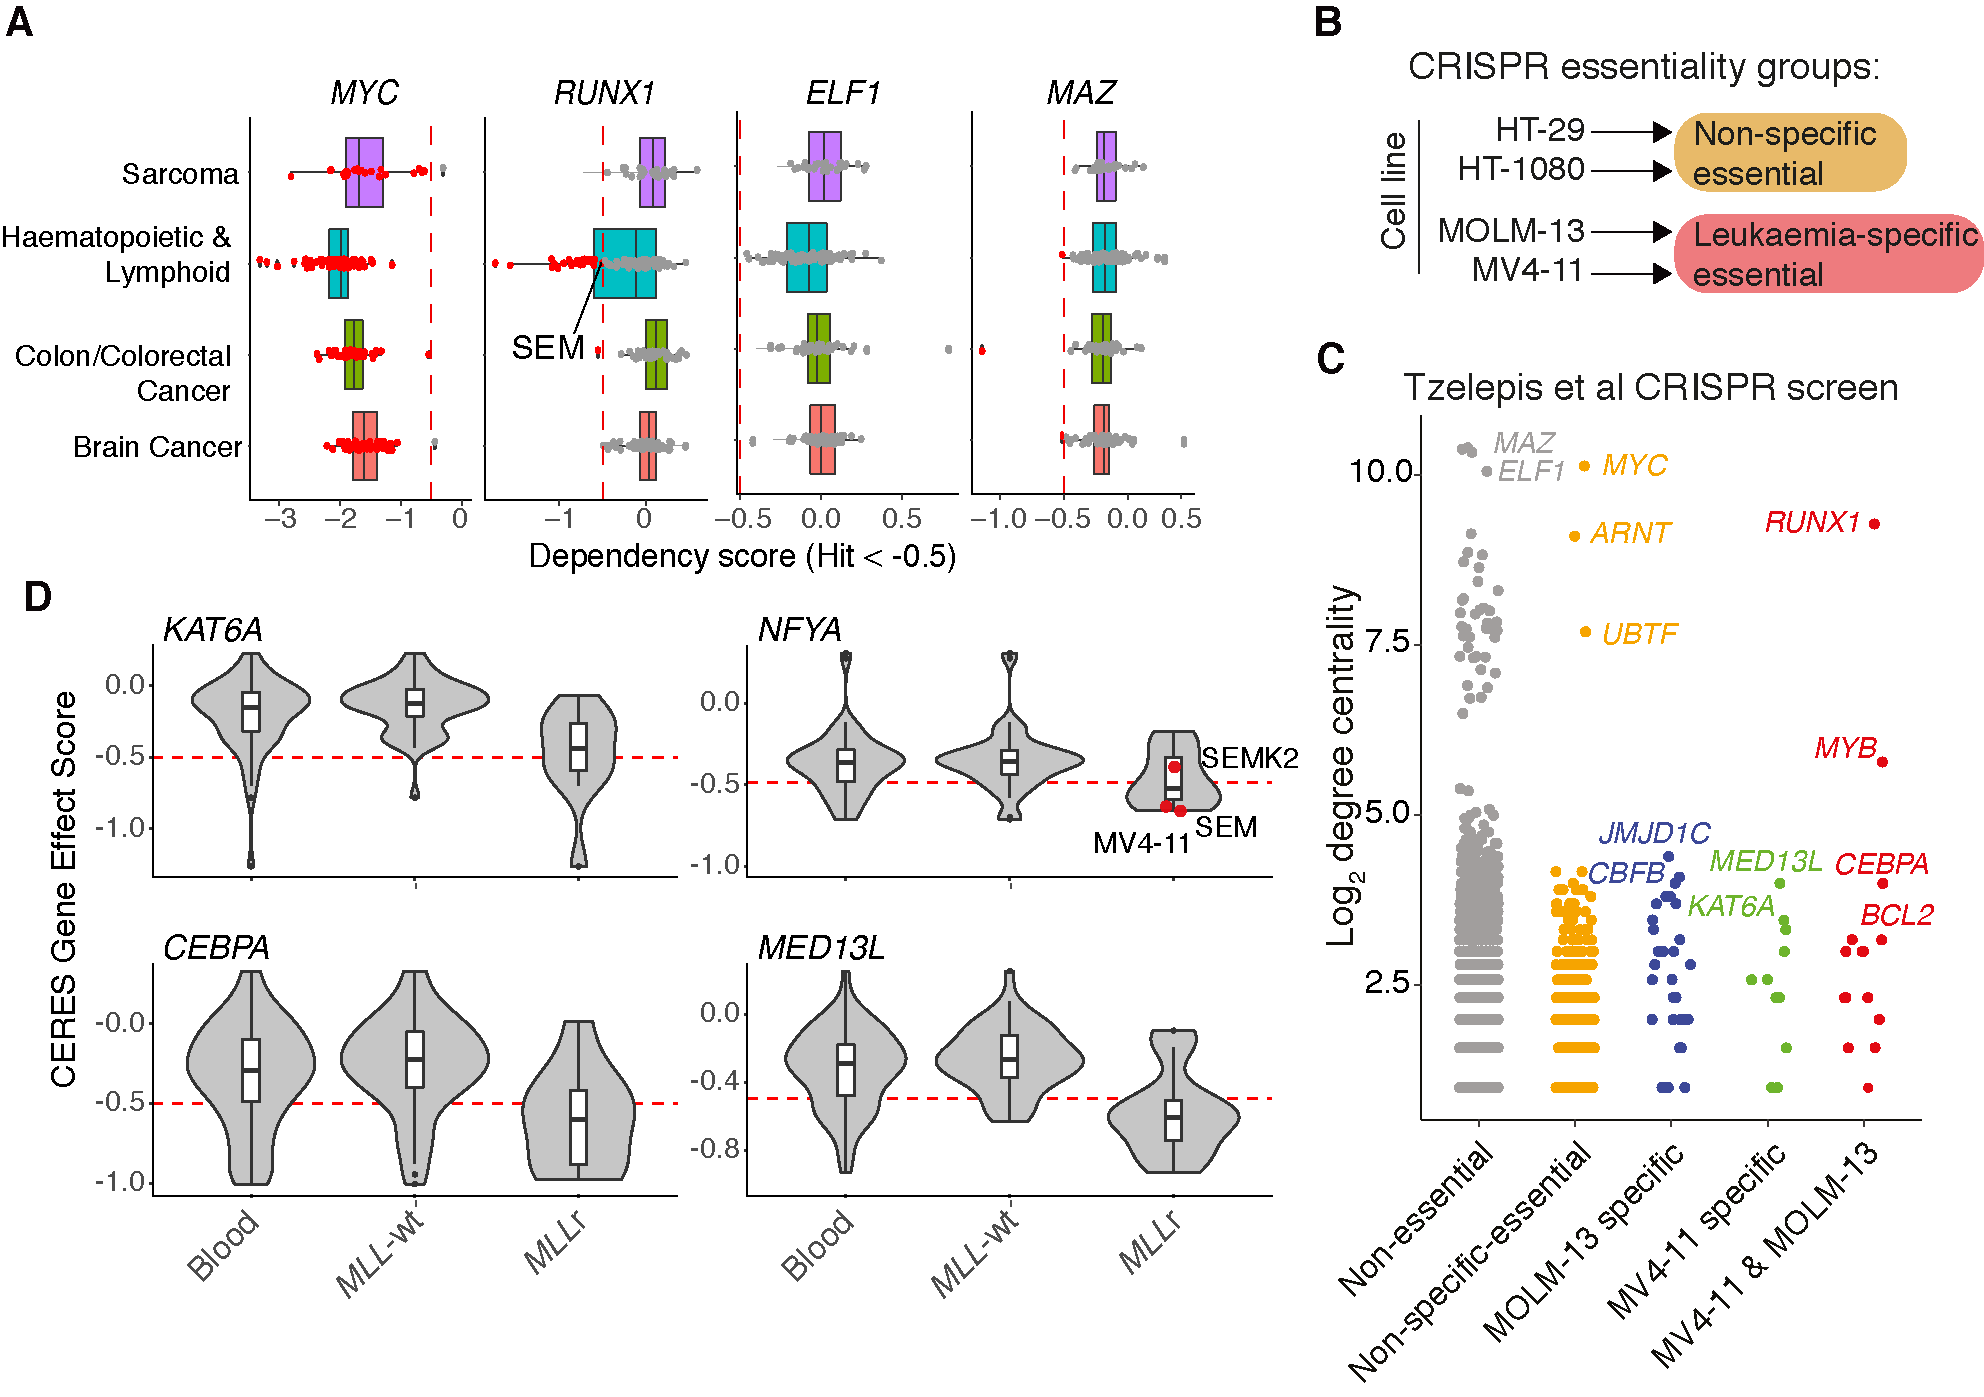
\includegraphics[width=\textwidth,height=\textheight,keepaspectratio]{figures/chapter4/ch4_essentiality.png}
    %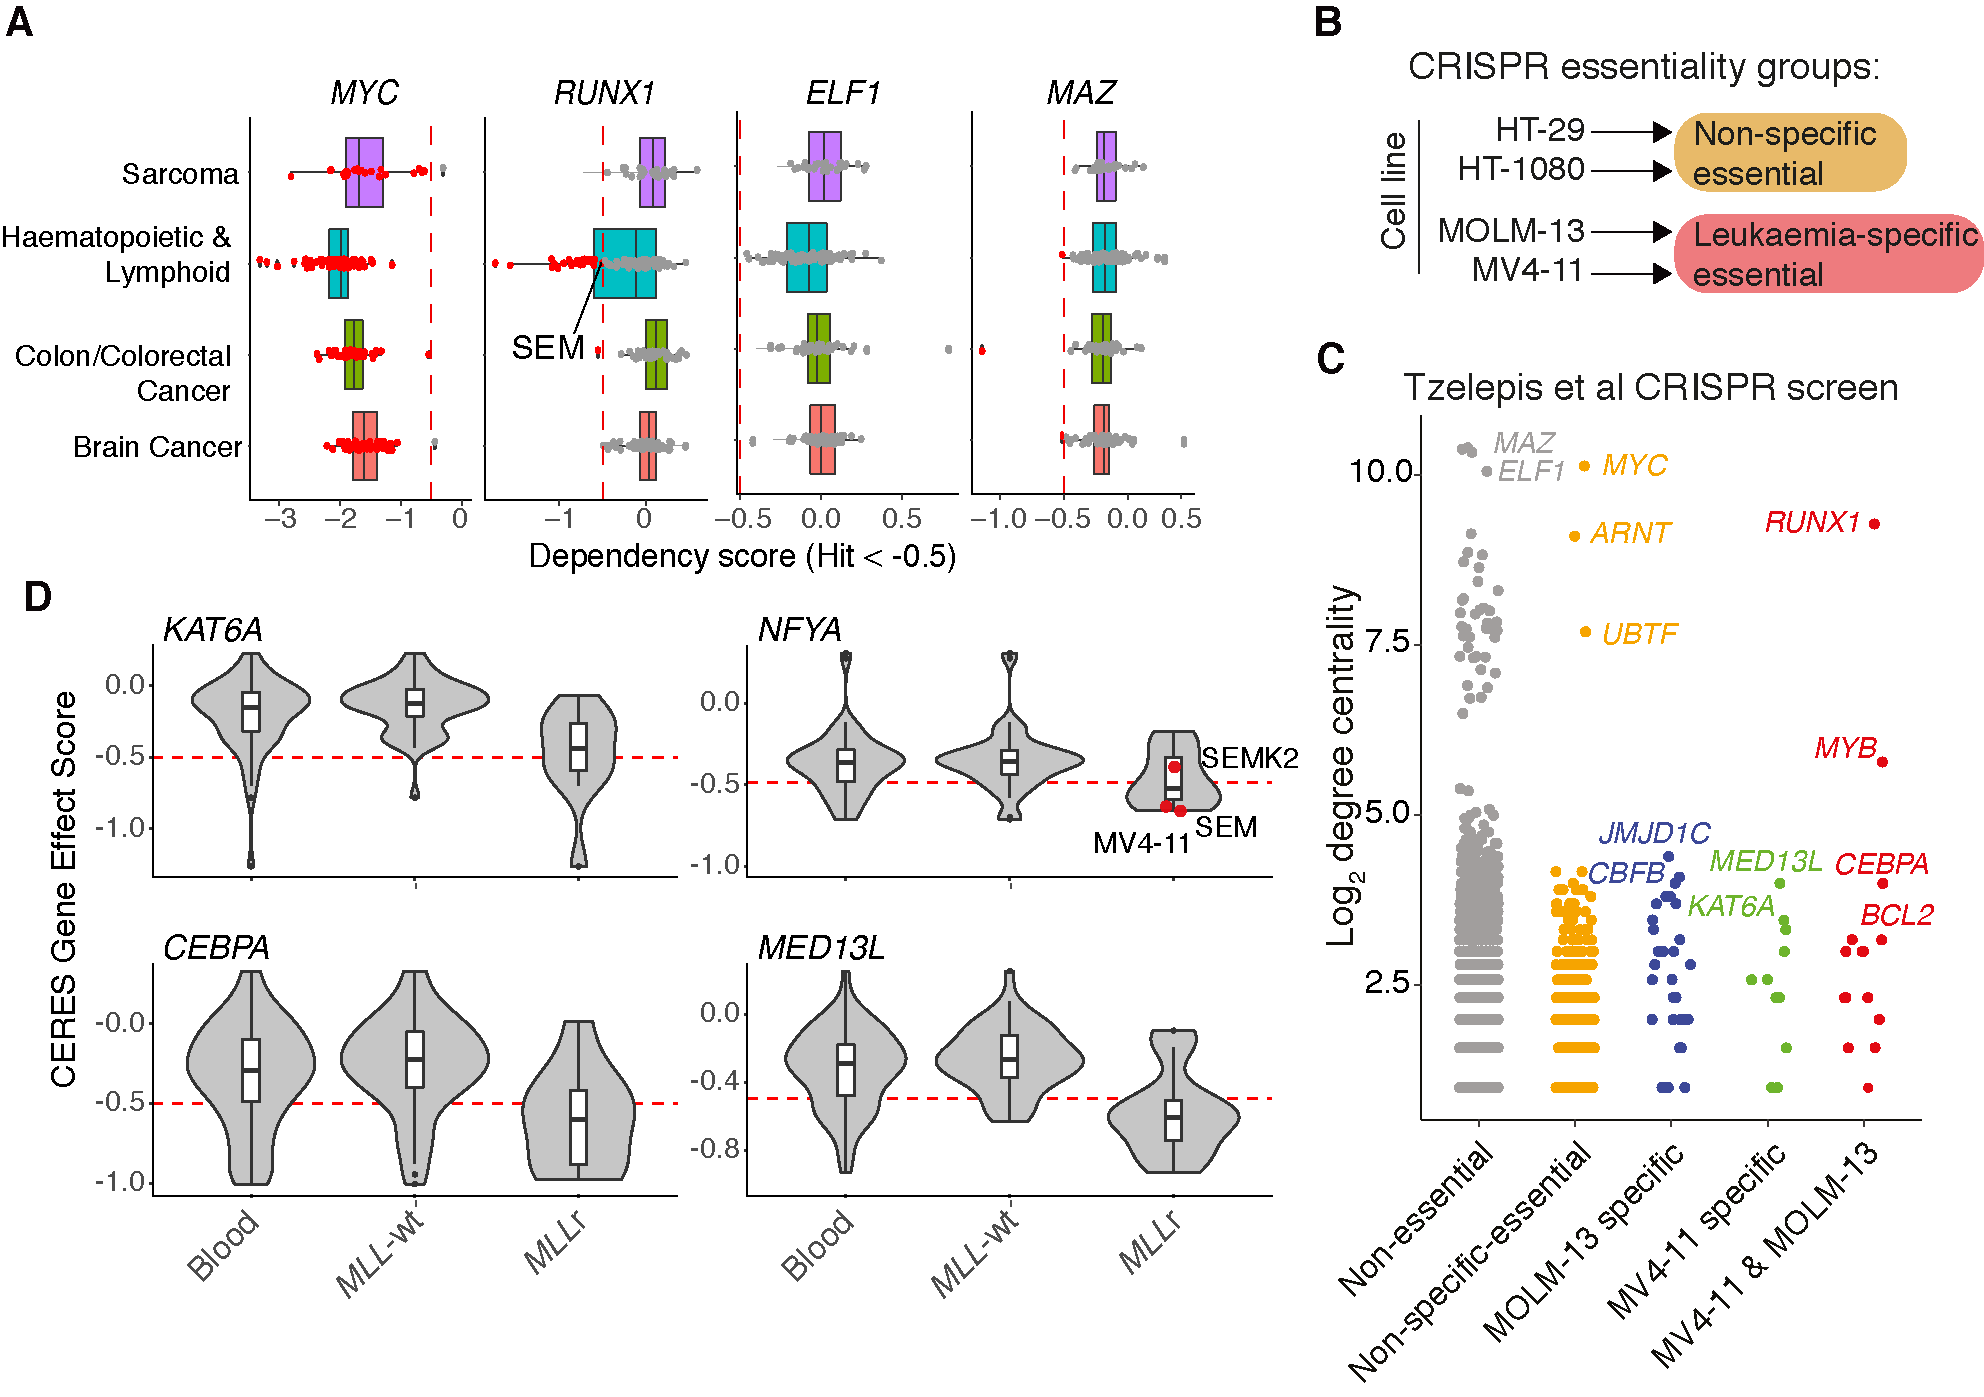
\includegraphics{figures/chapter4/ch4_essentiality.png}
    \caption[{Essential genes.}]
    {\textbf{CRISPR essentiality screens highlight RUNX1 as a critical central TF in MLL-FP leukaemias.} 
    \textbf{(A)} CRISPR essentiality CERES scores from DepMap (Avana 21Q1, \cite{meyers_computational_2017, doench_optimized_2016}). Genes are considered essential with a dependency score below -0.5. Each datapoint represents a different cell line, with essential hits highlighted red.
    \textbf{(B)} Illustration for how CRISPR essentiality screen hits from \cite{tzelepis_crispr_2016} are categorized. Essential genes in HT-29 or HT-1080 were "non-specific essential". Genes not essential in HT-29 or HT-1080 but essential in MOLM-13 or MV4-11 were specific to leukemia. 
    \textbf{(C)} Stratification of log\textsubscript{2} degree centrality (MLL-AF4 GRN) by CRISPR essentiality groups as outlined in B. 
    \textbf{(D)} CERES scores in haematopoietic cancer cell lines from DepMap, stratified by MLL translocation status. Red datapoints for \textit{NFYA} indicate MLL-AF4 cell lines. 
    \textit{Analysis in D performed by T. Wilson, supervised by me. CRISPR scores sourced from DepMap and \cite{tzelepis_crispr_2016}. Adapted from \cite{harman_kmt2a-aff1_2021}.} 
    }
    \label{fig:ch4_essentiality}
\end{figure}

To validate whether central TFs are important for leukaemogenesis, I integrated publicly available CRISPR essentiality screens. The Cancer Dependency Map (DepMap, Avana 21Q1 dataset, \cite{meyers_computational_2017, doench_optimized_2016}) found \textit{MYC} to be pan-essential, \textit{RUNX1} to be essential in multiple haematopoietic cancer models, and \textit{ELF1} and \textit{MAZ} to be non-essential (Fig. \ref{fig:ch4_essentiality}A). As this is a large and generalised screen, I integrated a more targeted screen from \cite{tzelepis_crispr_2016} which includes two \textit{MLL}r cell lines, MOLM-13 (MLL-AF9 AML) and MV4-11 (MLL-AF4 AML), alongside two non-leukaemic cancer cell lines, HT-29 (colon adenocarcinoma) and HT-1080 (fibrosarcoma). To find genes essential specifically in leukaemia, hits were categorised as non-essential, non-specific essential (hit in HT-29 or HT-1080), or essential in one or both \textit{MLL}r leukaemias (hit in MOLM-13 and/or MV4-11, but not HT-29 or HT-1080) (Fig. \ref{fig:ch4_essentiality}B-C). In line with the DepMap data, \textit{MYC} was pan-essential, while \textit{MAZ} and \textit{ELF1} were not essential in any cell line. This suggests \textit{MAZ} and \textit{ELF1}, while highly connected, are not important for survival or proliferation, at least in AML. \textit{RUNX1} was essential in both MOLM-13 and MV4-11 cells, highlighting its importance under the control of both MLL-AF4 and -AF9 fusion proteins. Other central leukaemia-specific hits include \textit{MYB}, \textit{MED13L}, \textit{CEBPA}, and \textit{KAT6A} (Fig. \ref{fig:ch4_essentiality}C). 

The MV4-11 and MOLM-13 essential gene \textit{CEBPA}, along with the MV4-11 specific hits \textit{MED13L} and \textit{KAT6A}, show greater essentiality for \textit{MLL}r samples over non-\textit{MLL}r blood cancers (Fig. \ref{fig:ch4_essentiality}D). NF-YA is a central (but not core to all MLL-FPs) node in the GRN and is not significantly essential in the \cite{tzelepis_crispr_2016} screen. However, the DepMap screen shows higher essentiality for NF-YA in \textit{MLL}r samples, with \textit{MLL-AF4} cell lines (SEM and MV4-11) showing the high essentiality (Fig. \ref{fig:ch4_essentiality}D). This indicates that not only are these genes essential for MLL\textit{r} AML, but show generally greater essentiality for \textit{MLL}r leukaemias than other haematopoietic malignancies, possibly in part as a core-program targeted by all MLL-FPs. Overall, this analysis shows that degree centrality highlights many essential genes, and identifying high centrality in TFs critical for both MLL-AF4 and MLL-AF9 AML.

\subsection{\label{ch4:stress-centrality}Stress is a better indicator of essentiality than degree centrality}

As demonstrated, while degree centrality highlights nodes that regulate a wide range of targets and are often critical, this measure does not always translate into essentiality for leukaemic cells. Stress centrality (a variant of betweenness centrality) may better reflect essentiality, as it represents nodes less likely to be compensated for upon perturbation (see introduction section \ref{ch1:centrality}, p.\pageref{ch1:centrality}, Fig. \ref{fig:ch1_stress-example}). In fact, while there is a slight enrichment in degree centrality for MV4-11 essential genes, there is much higher stress centrality observed in MV4-11 essential genes over non-essential genes (Fig. \ref{fig:ch4_centrality}A). \textit{MAZ} was a non-essential TF, which despite high connectivity, shows relatively low stress centrality than comparably connected TFs (Fig. \ref{fig:ch4_centrality}B). Exploring the ratio between stress and degree centrality, RUNX1 has a far higher stress for its connectivity than other TFs (degree 636, stress 80864), and while MYB is not highly connected it also shows a very high stress:degree ratio (degree 56, stress 3797) (Fig. \ref{fig:ch4_centrality}C). It has been suggested that nodes with low degree and high stress are particularly important factors for connecting network modules \citep{joy_high-betweenness_2005, koschutzki_centrality_2008}, placing RUNX1 as a critical TF in bridging interactions between factors, such as MLL-AF4.

\begin{figure}[!t]
    \centering
    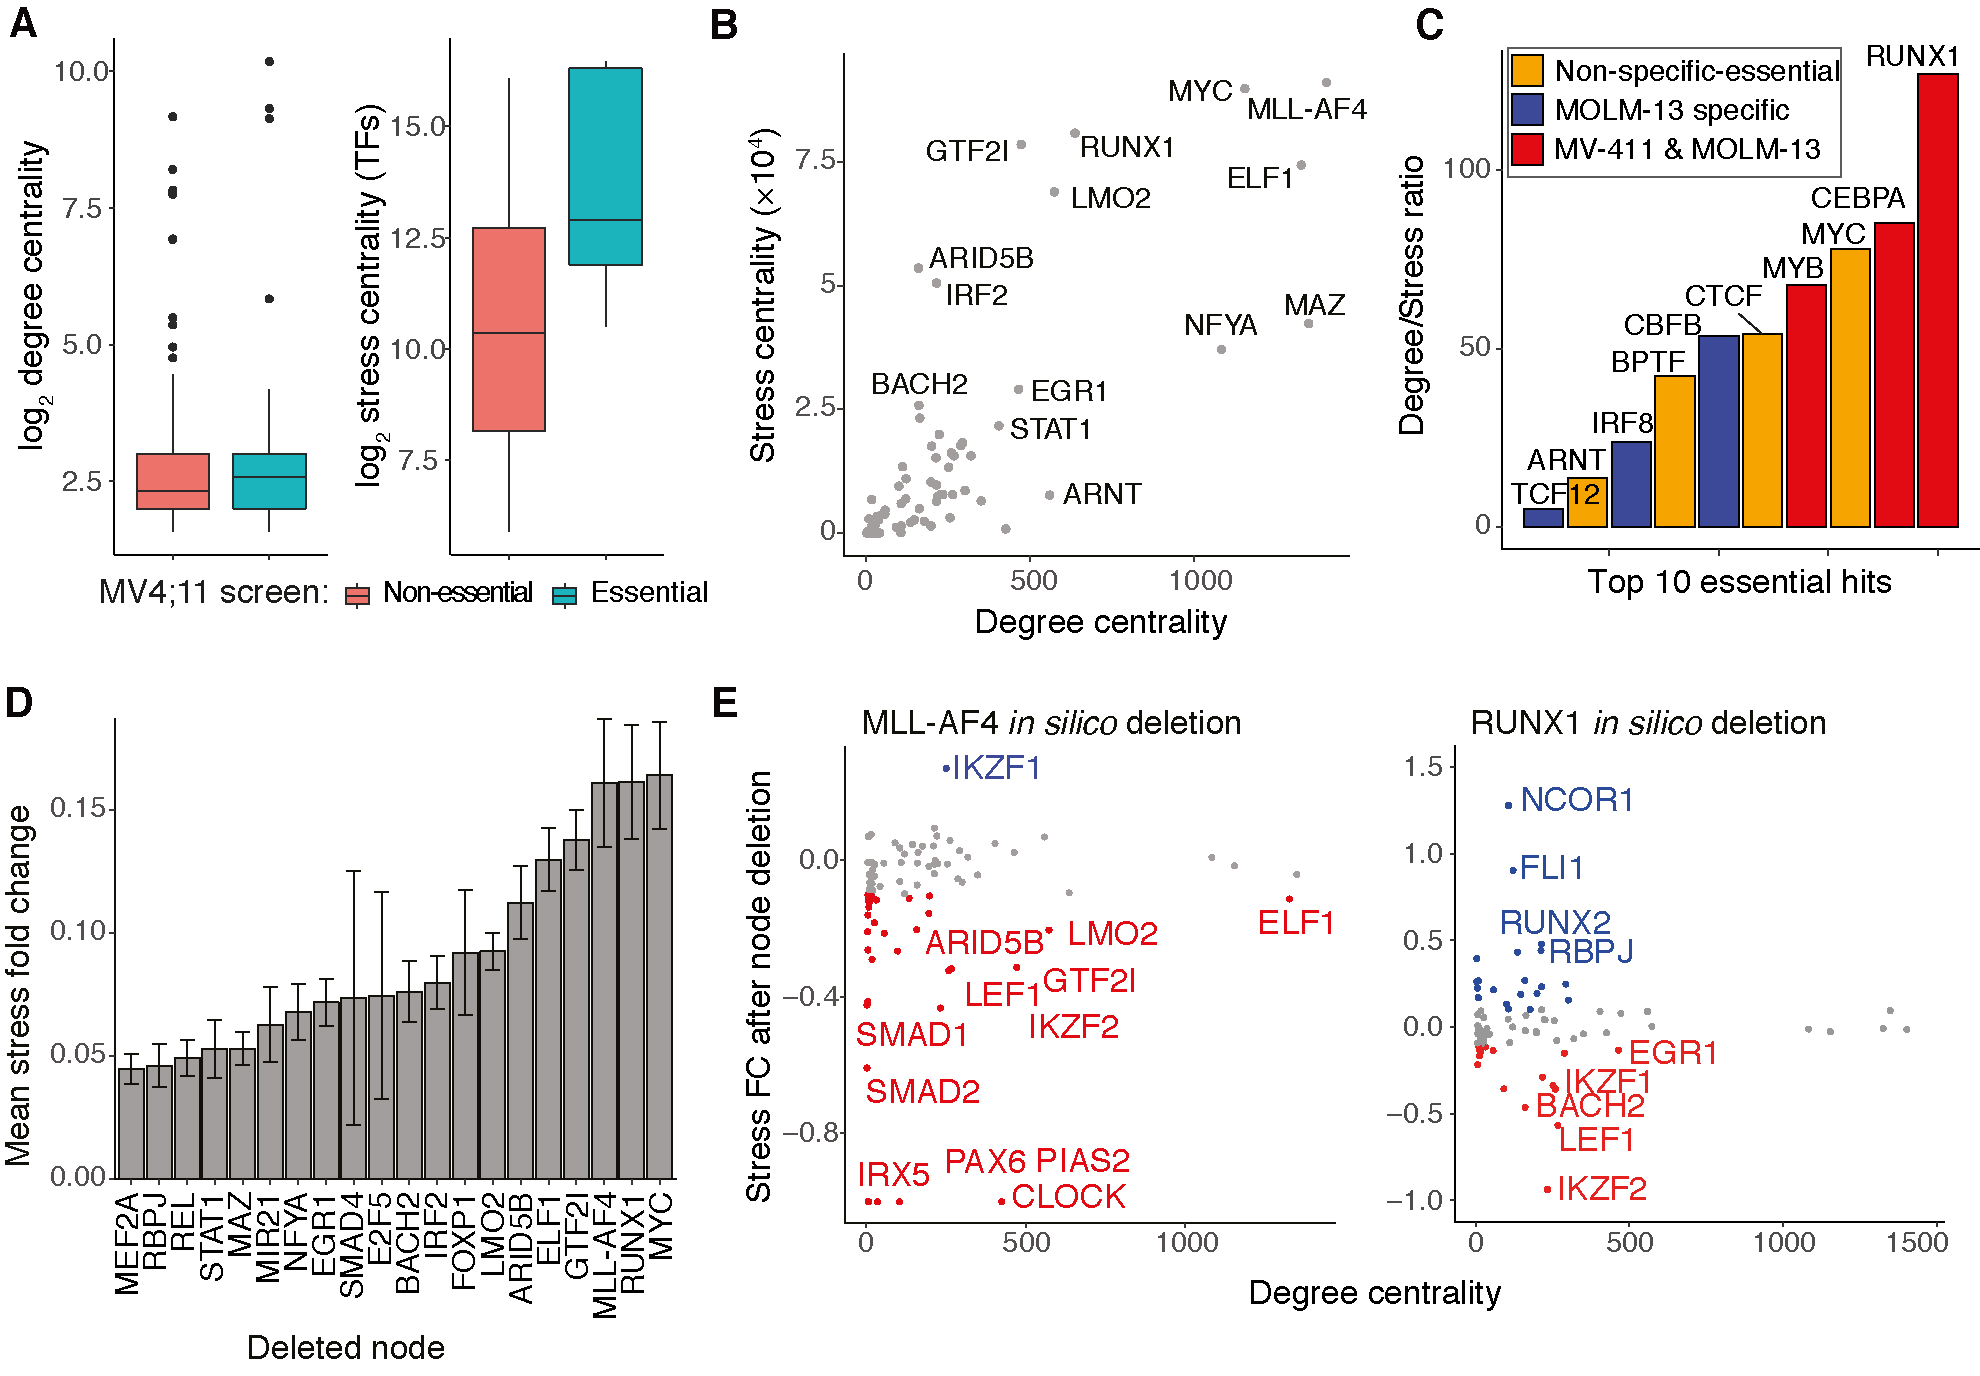
\includegraphics[width=\textwidth,height=\textheight,keepaspectratio]{figures/chapter4/ch4_centrality.png}
    %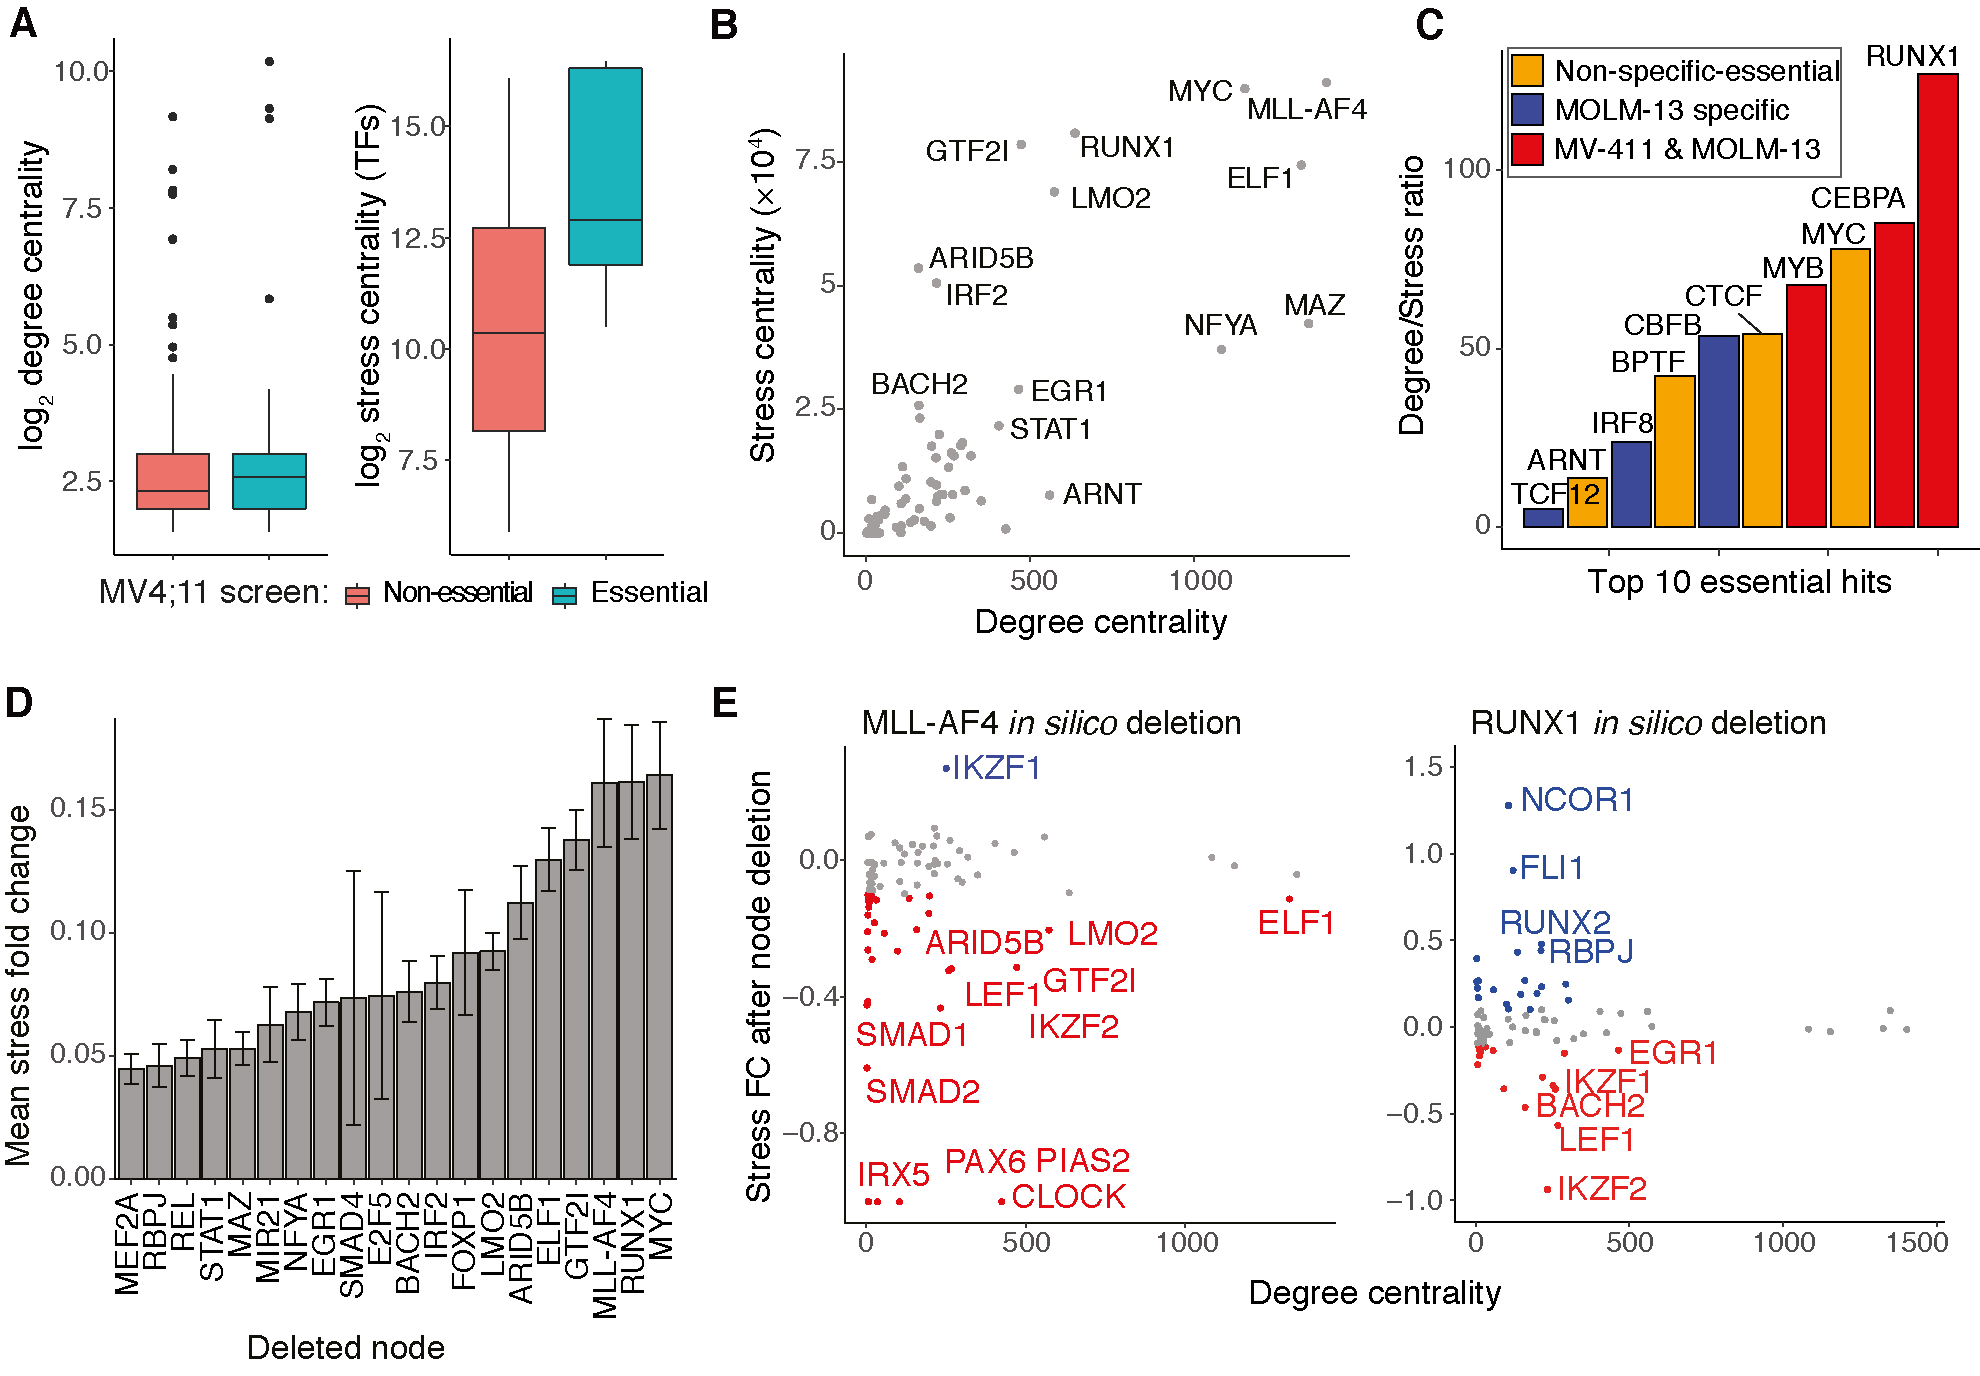
\includegraphics{figures/chapter4/ch4_centrality.png}
    \caption[{Centrality analysis of MLL-AF4 GRN.}]
    {\textbf{Centrality analysis of MLL-AF4 GRN.} 
    \textbf{(A)} Log\textsubscript{2} degree and stress centrality of the MLL-AF4 GRN nodes plotted by MV4-11 essentiality from \cite{tzelepis_crispr_2016}. 
    \textbf{(B)} Relationship between degree and stress centrality of MLL-AF4 GRN nodes. 
    \textbf{(C)} Rank order plot of ratios between stress and degree centrality for ten most essential GRN hubs from \cite{tzelepis_crispr_2016}. 
    \textbf{(D)} Top 20 in silico deleted nodes by mean stress FC (methods section \ref{ch2:centrality}, p.\pageref{ch2:centrality}). 
    \textbf{(E)} Stress FC after in silico deletion of RUNX1 or MLL-AF4, plotted against degree centrality. Blue and red indicate positive (FC > 0.1) and negative (FC < -0.1) stress FC, respectively. 
    \textit{Adapted from \cite{harman_kmt2a-aff1_2021}.}
    }
    \label{fig:ch4_centrality}
\end{figure}

As discussed, central TFs may contain redundant regulatory logic that compensates for specific perturbation. To investigate alternative nodes that may facilitate TF compensation, I established an approach where each GRN node was deleted in silico, and stress centrality values recalculated. Stress values before and after in silico deletion were compared as stress fold change (stress FC), and summarised for every node (Fig. \ref{fig:ch4_centrality}D). RUNX1 and MYC in silico deletion showed the greatest stress redistribution, above MLL-AF4, while the non-essential factors MAZ and NFYA show less stress FC redistribution (Fig. \ref{fig:ch4_centrality}D). Looking in detail, MLL-AF4 deletion results in negative stress FC while RUNX1 shows positive and negative stress FC. RUNX1 in silico deletion shows increased NCOR1, FLI1, RBPJ and RUNX2 stress, while factors such as IKZF1 and IKZF2 are reduced (Fig. \ref{fig:ch4_centrality}E), indicating that these TFs provide an alternative route to reach RUNX1 target nodes. RUNX2 is expected as it shares the RUNT domain with RUNX1, and therefore can likely compensate for perturbation. RUNX1 has been shown to cooperate with FLI1, altering its binding affinity for the FLI1 motif and remodelling FLI1 regulatory logic \citep{gilmour_co-operation_2018, lichtinger_runx1_2012}. RBPJ is a transcriptional repressor, yet forms a transactivating complex with NOTCH intracellular domain (NICD) \citep{kojika_notch_2001}. RUNX1 and RBPJ-NICD cooperate at specific loci, for example to coregulate the +1.27 Mb \textit{MYC} enhancer and \textit{IL7R} enhancers \citep{choi_runx1_2017, wang_notch1-rbpj_2014}. This cooperative behaviour is indicative of shared regulatory logic, and while these factors function in combination, it is likely they regulate common sites in the absence of RUNX1. Genes that decrease in stress may reflect a breakdown in network pathways. For example, if node pairs must communicate through a RUNX1:IKZF1 axis then loss of RUNX1 will break down the path of communication via IKZF1. This places IKZF1 as a key target of RUNX1, required for downstream communication within the network. This lines up with Runx1 regulation of Ikzf1 in EHT, which was predicted to enact TF cascades to repress Notch genes (Fig. \ref{fig:ch3_runx1-ikzf1-notch}D, p.\pageref{fig:ch3_runx1-ikzf1-notch}). This analysis serves to rank nodes based on stress centrality, which may better reflect importance, and predicts compensatory mechanisms upon perturbation. In particular it highlights RUNX1, MYB, CEBPA and MYC as highly important TFs, and notes potential redundancy between RUNX1 and specific factors at a subset of targets. 

\section{\label{ch4:mll-af4-runx1}MLL-AF4 and RUNX1 cooperate to regulate gene expression}

\subsection{Generating, and characterising a RUNX1 driven GRN model of leukaemia}

\begin{figure}[!b]
    \centering
    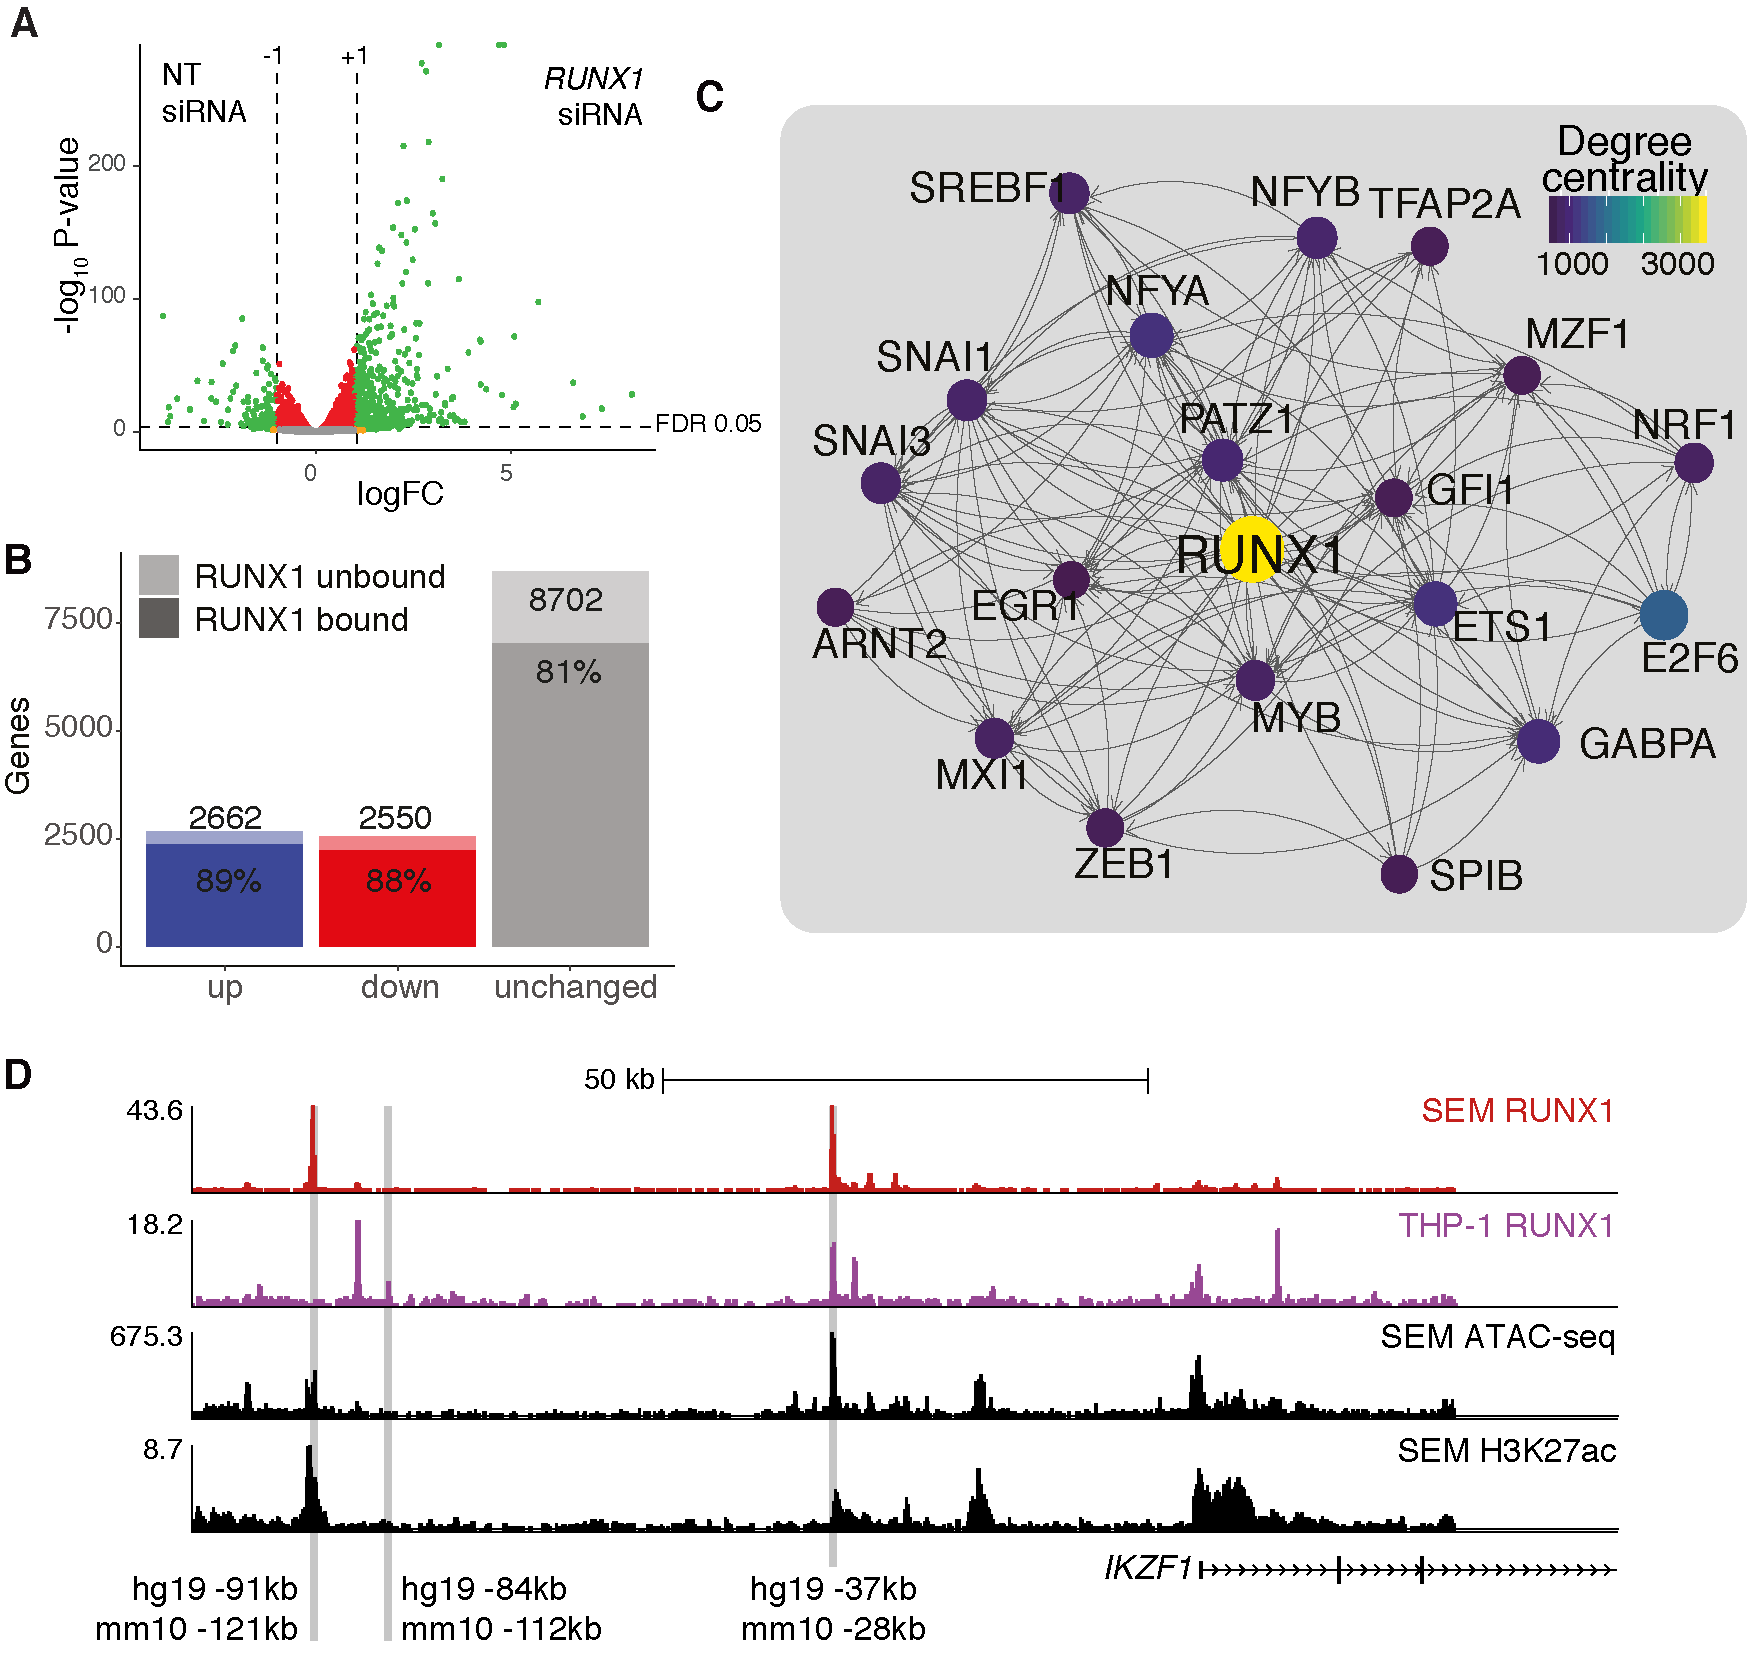
\includegraphics[width=\textwidth,height=\textheight,keepaspectratio]{figures/chapter4/chr4_runx1-grn.png}
    %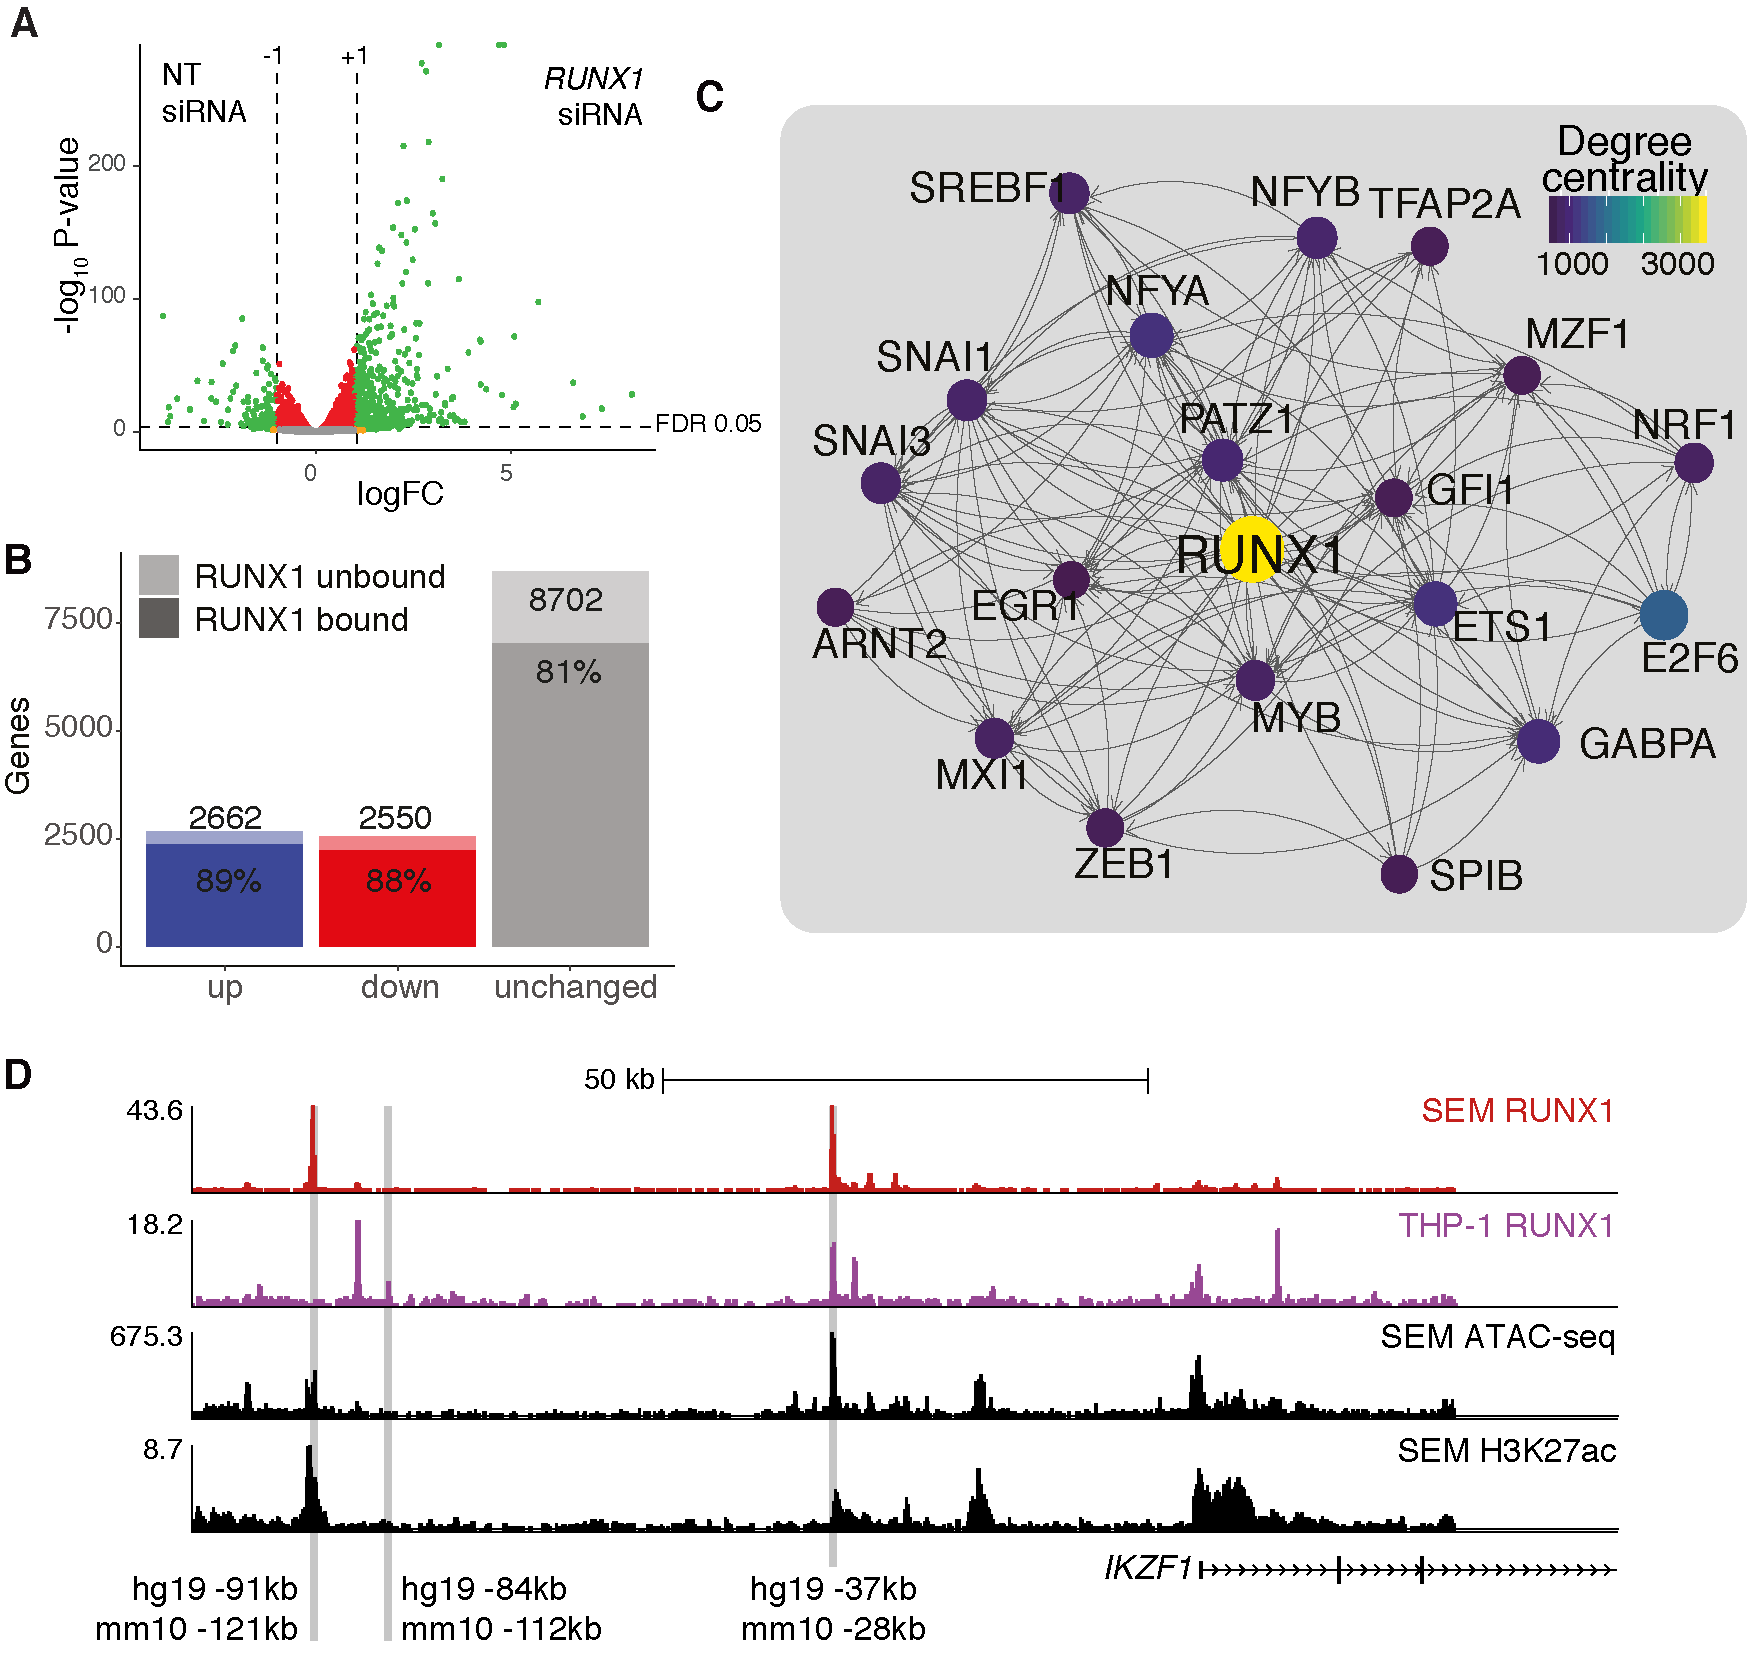
\includegraphics{figures/chapter4/chr4_runx1-grn.png}
    \caption[{Establishing a RUNX1 centred GRN in SEM cells.}]
    {\textbf{Establishing a RUNX1 centred GRN in SEM cells.} 
    \textbf{(A)} Relationship between -log\textsubscript{10} P value and logFC in \textit{RUNX1} KD nascent RNA-seq. Genes are coloured by logFC and FDR thresholds as indicated by dashed lines.
    \textbf{(B)} DEGs from nascent RNA-seq after 96 h \textit{RUNX1} KD (\textit{n} = 3). Shaded bar represents RUNX1-bound genes.
    \textbf{(C)} The top 20 genes of the RUNX1 GRN by degree centrality. Lines indicate predicted interaction from protein to gene locus, with arrowheads pointing downstream. 
    \textbf{(D)} ChIP-seq and ATAC-seq tracks at the human \textit{IKZF1} locus. Mouse -28, -112, and -121 enhancers are highlighted, matched by sequence similarity using UCSC BLAT. 
    \textit{Raw nascent RNA-seq data was generated by M. Tapia (Milne lab) and analysed by me. Adapted from \cite{harman_kmt2a-aff1_2021}.}
    } 
    \label{fig:ch4_runx1-grn}
\end{figure}

To begin to address how MLL-AF4 regulates a wider network in combination with TFs, I selected RUNX1 as an example of a critical MLL-AF4 activated node. Across multiple analyses RUNX1 was promoted as a critical TF within the MLL-AF4 GRN, it is highly central and is a core-TF active in both MLL-AF4 ALL and MLL-AF9 AML. To understand RUNX1 regulatory logic in detail, I established a RUNX1-centred GRN. Nascent RNA-seq data following 96 hours' \textit{RUNX1} KD generated by M. Tapia revealed 5212 DEGs, the majority of which were bound by RUNX1 (Fig. \ref{fig:ch4_runx1-grn}A-B). A RUNX1-centric GRN was established using this nascent RNA-seq and previously published RUNX1 ChIP-seq \citep{wilkinson_runx1_2013}, using the same approach as in Fig. \ref{fig:ch4_ma4-grn}. Many known targets of RUNX1, such as \textit{GFI1} \citep{wilson_gfi1_2010} and \textit{MYB} \citep{choi_runx1_2017}, were central to the RUNX1 GRN (Fig. \ref{fig:ch4_runx1-grn}C). A number of Runx1 targets in the EHT GRN (see section \ref{ch3:runx1-targets}, p.\pageref{ch3:runx1-targets}) are also present here, including, among others, \textit{MYB}, \textit{IKZF1/2}, \textit{SNAI1/3}, \textit{ZEB1/2}, \textit{GFI1} and the NOTCH targets \textit{HES1}, \textit{HEY1} and \textit{HEY2}. I compared RUNX1 binding at the \textit{IKZF1} locus with the EHT GRN and the mouse predicted enhancer elements (Fig. \ref{fig:ch3_runx1-ikzf1}, p.\pageref{fig:ch3_runx1-ikzf1}). RUNX1 binding at \textit{IKZF1} shows similar occupancy of the -28 and -121 enhancer elements (-37 kb and -91 kb in human) as in EHT, though the -112 enhancer (-84 kb in human) is not bound by RUNX1 (Fig. \ref{fig:ch4_runx1-grn}D). This suggests both GRN models capture common RUNX1 regulatory logic, though with some differences in enhancer occupancy, that is preserved across species and between different cell contexts.

\subsection[RUNX1 and MLL-AF4 GRNs intersect at leukaemogenic processes]{RUNX1 and MLL-AF4 GRNs intersect at\\leukaemogenic processes}

\begin{figure}[!t]
    \centering
    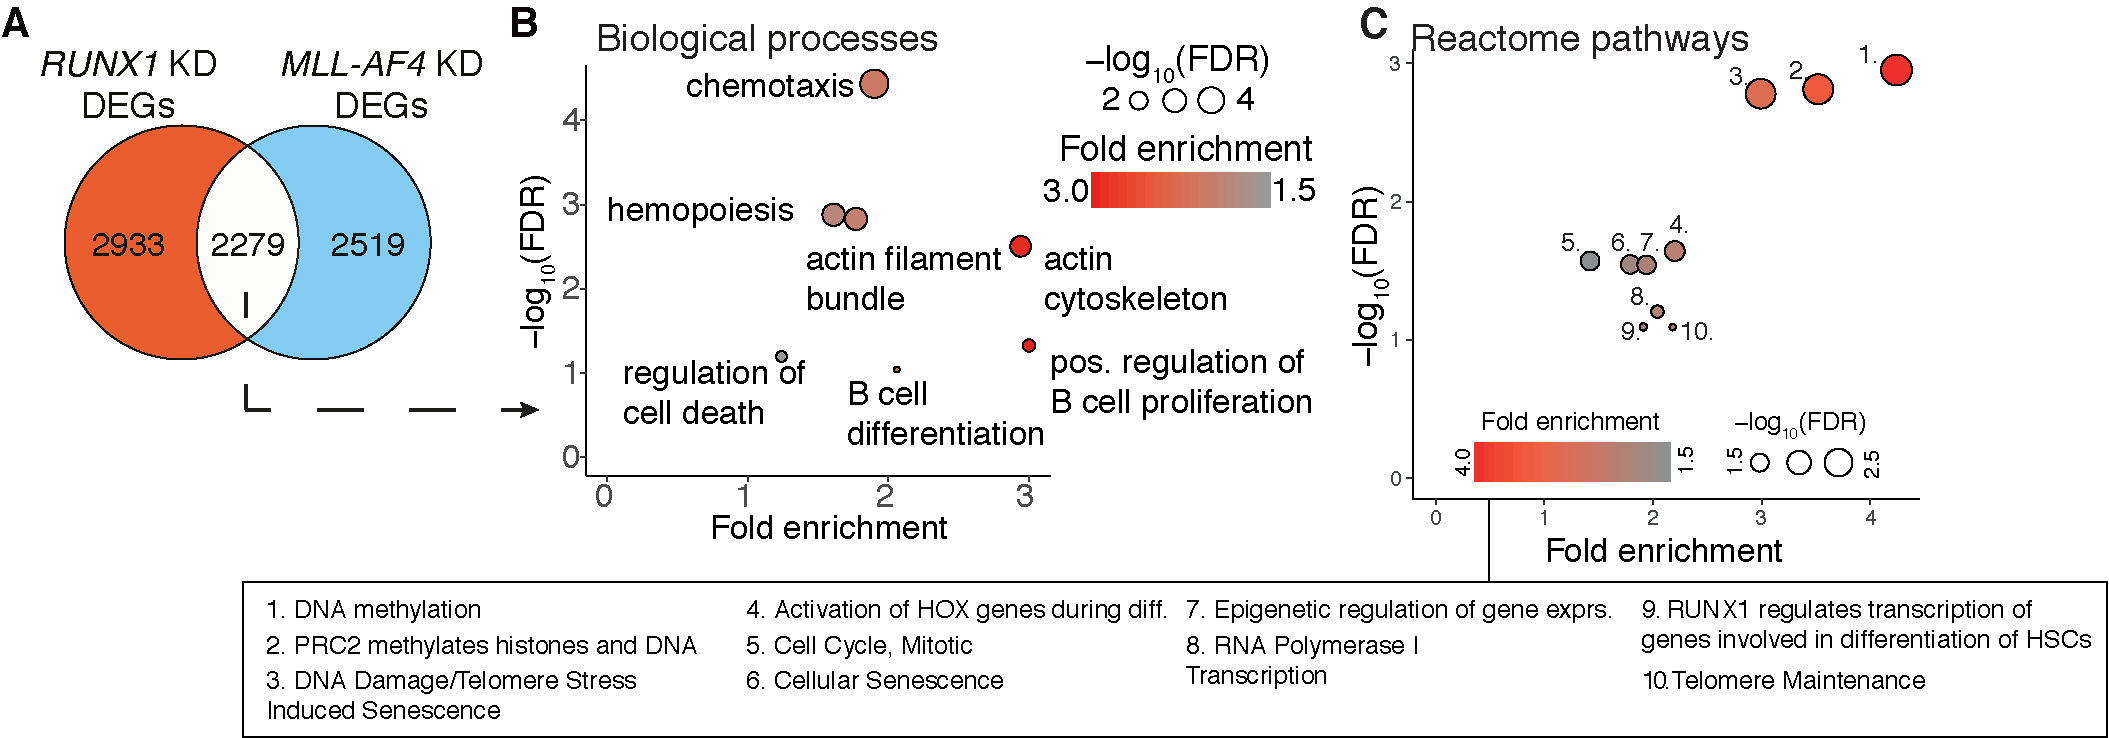
\includegraphics[width=\textwidth,height=\textheight,keepaspectratio]{figures/chapter4/chr4_interplay.png}
    %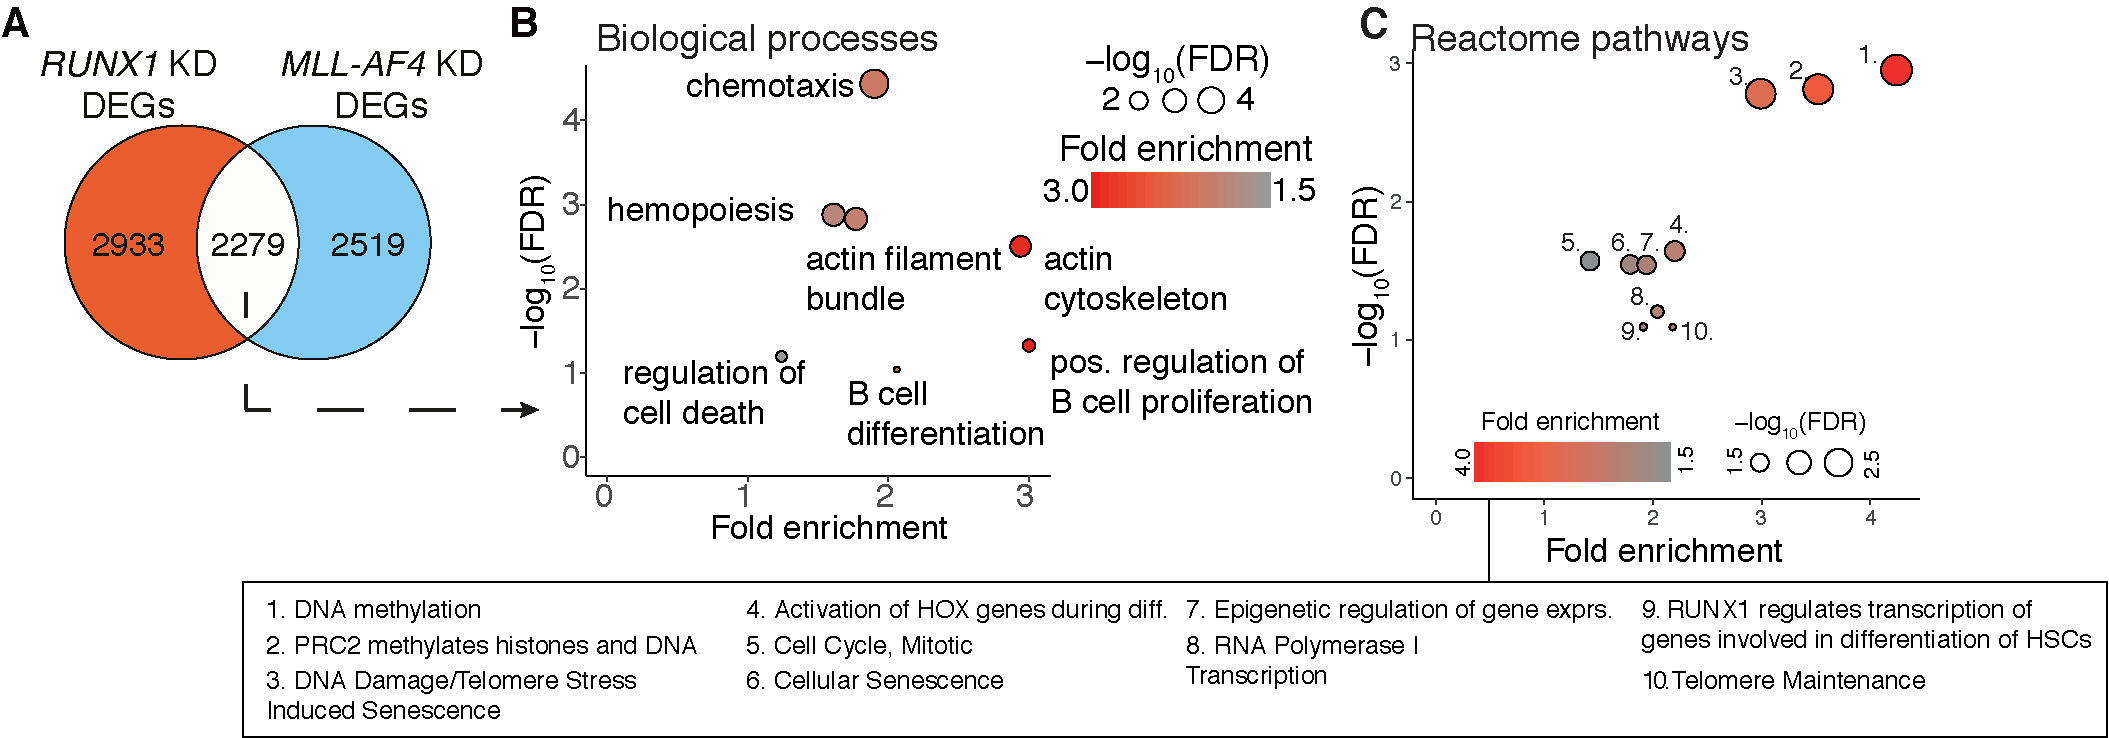
\includegraphics{figures/chapter4/chr4_interplay.png}
    \caption[{The overlap between MLL-AF4 and RUNX1 GRNs is enriched for processes promoting leukaemogenesis.}]
    {\textbf{The overlap between MLL-AF4 and RUNX1 GRNs is enriched for processes promoting leukaemogenesis.} 
    %\textbf{(A)} Distribution of logFC expression response to \textit{MLL-AF4} KD, \textit{RUNX1} KD, or EPZ-5675 treatment. LogFC response stratified by GRN-predicted direct or indirect regulation by MLL-AF4. 
    %\textbf{(B)} Reference-normalized ChIP-seq tracks for MLL-N and RUNX1 after 48 hours’ \textit{RUNX1} KD. 
    \textbf{(A)} Overlap between \textit{MLL-AF4} KD DEGs (Fig. \ref{fig:ch4_GRN_just}A) and RUNX1 KD DEGs (Fig. \ref{fig:ch4_runx1-grn}A-B). 
    \textbf{(B-C)} GO biological process (B) and reactome pathway (C) enrichment for overlap shown in A. 
    \textit{Adapted from \cite{harman_kmt2a-aff1_2021}.}
    }
    \label{fig:ch4_interplay}
\end{figure}

The central hypothesis of this chapter is that MLL-AF4 regulates a wider network through driving RUNX1 expression (Fig. \ref{fig:ch4_GRN_just}B), and the analysis so far has identified the TF RUNX1 as a key downstream effector of MLL-AF4 activity. Genes that are sensitive to both \textit{MLL-AF4} and \textit{RUNX1} KD in the GRN models (2279 DEGs, Fig. \ref{fig:ch4_interplay}A) were enriched for processes related to haematopoiesis, regulation of cell death, and B cell proliferation, consistent with an ALL expression program (Fig. \ref{fig:ch4_interplay}C). Pathway enrichment of these co-regulated genes revealed terms for epigenetic regulation such as DNA and histone methylation, cell cycle, and RUNX1 regulation (Fig. \ref{fig:ch4_interplay}C). These analyses suggest that the intersection of MLL-AF4 and RUNX1 GRNs drive a pro-leukaemic program.

\section{\label{ch4:ma4-runx1}MLL-AF4 and RUNX1 direct both FFL and TF cascade regulation}

\subsection{Identifying FFL and cascade regulatory circuits}

\begin{figure}[!t]
    \centering
    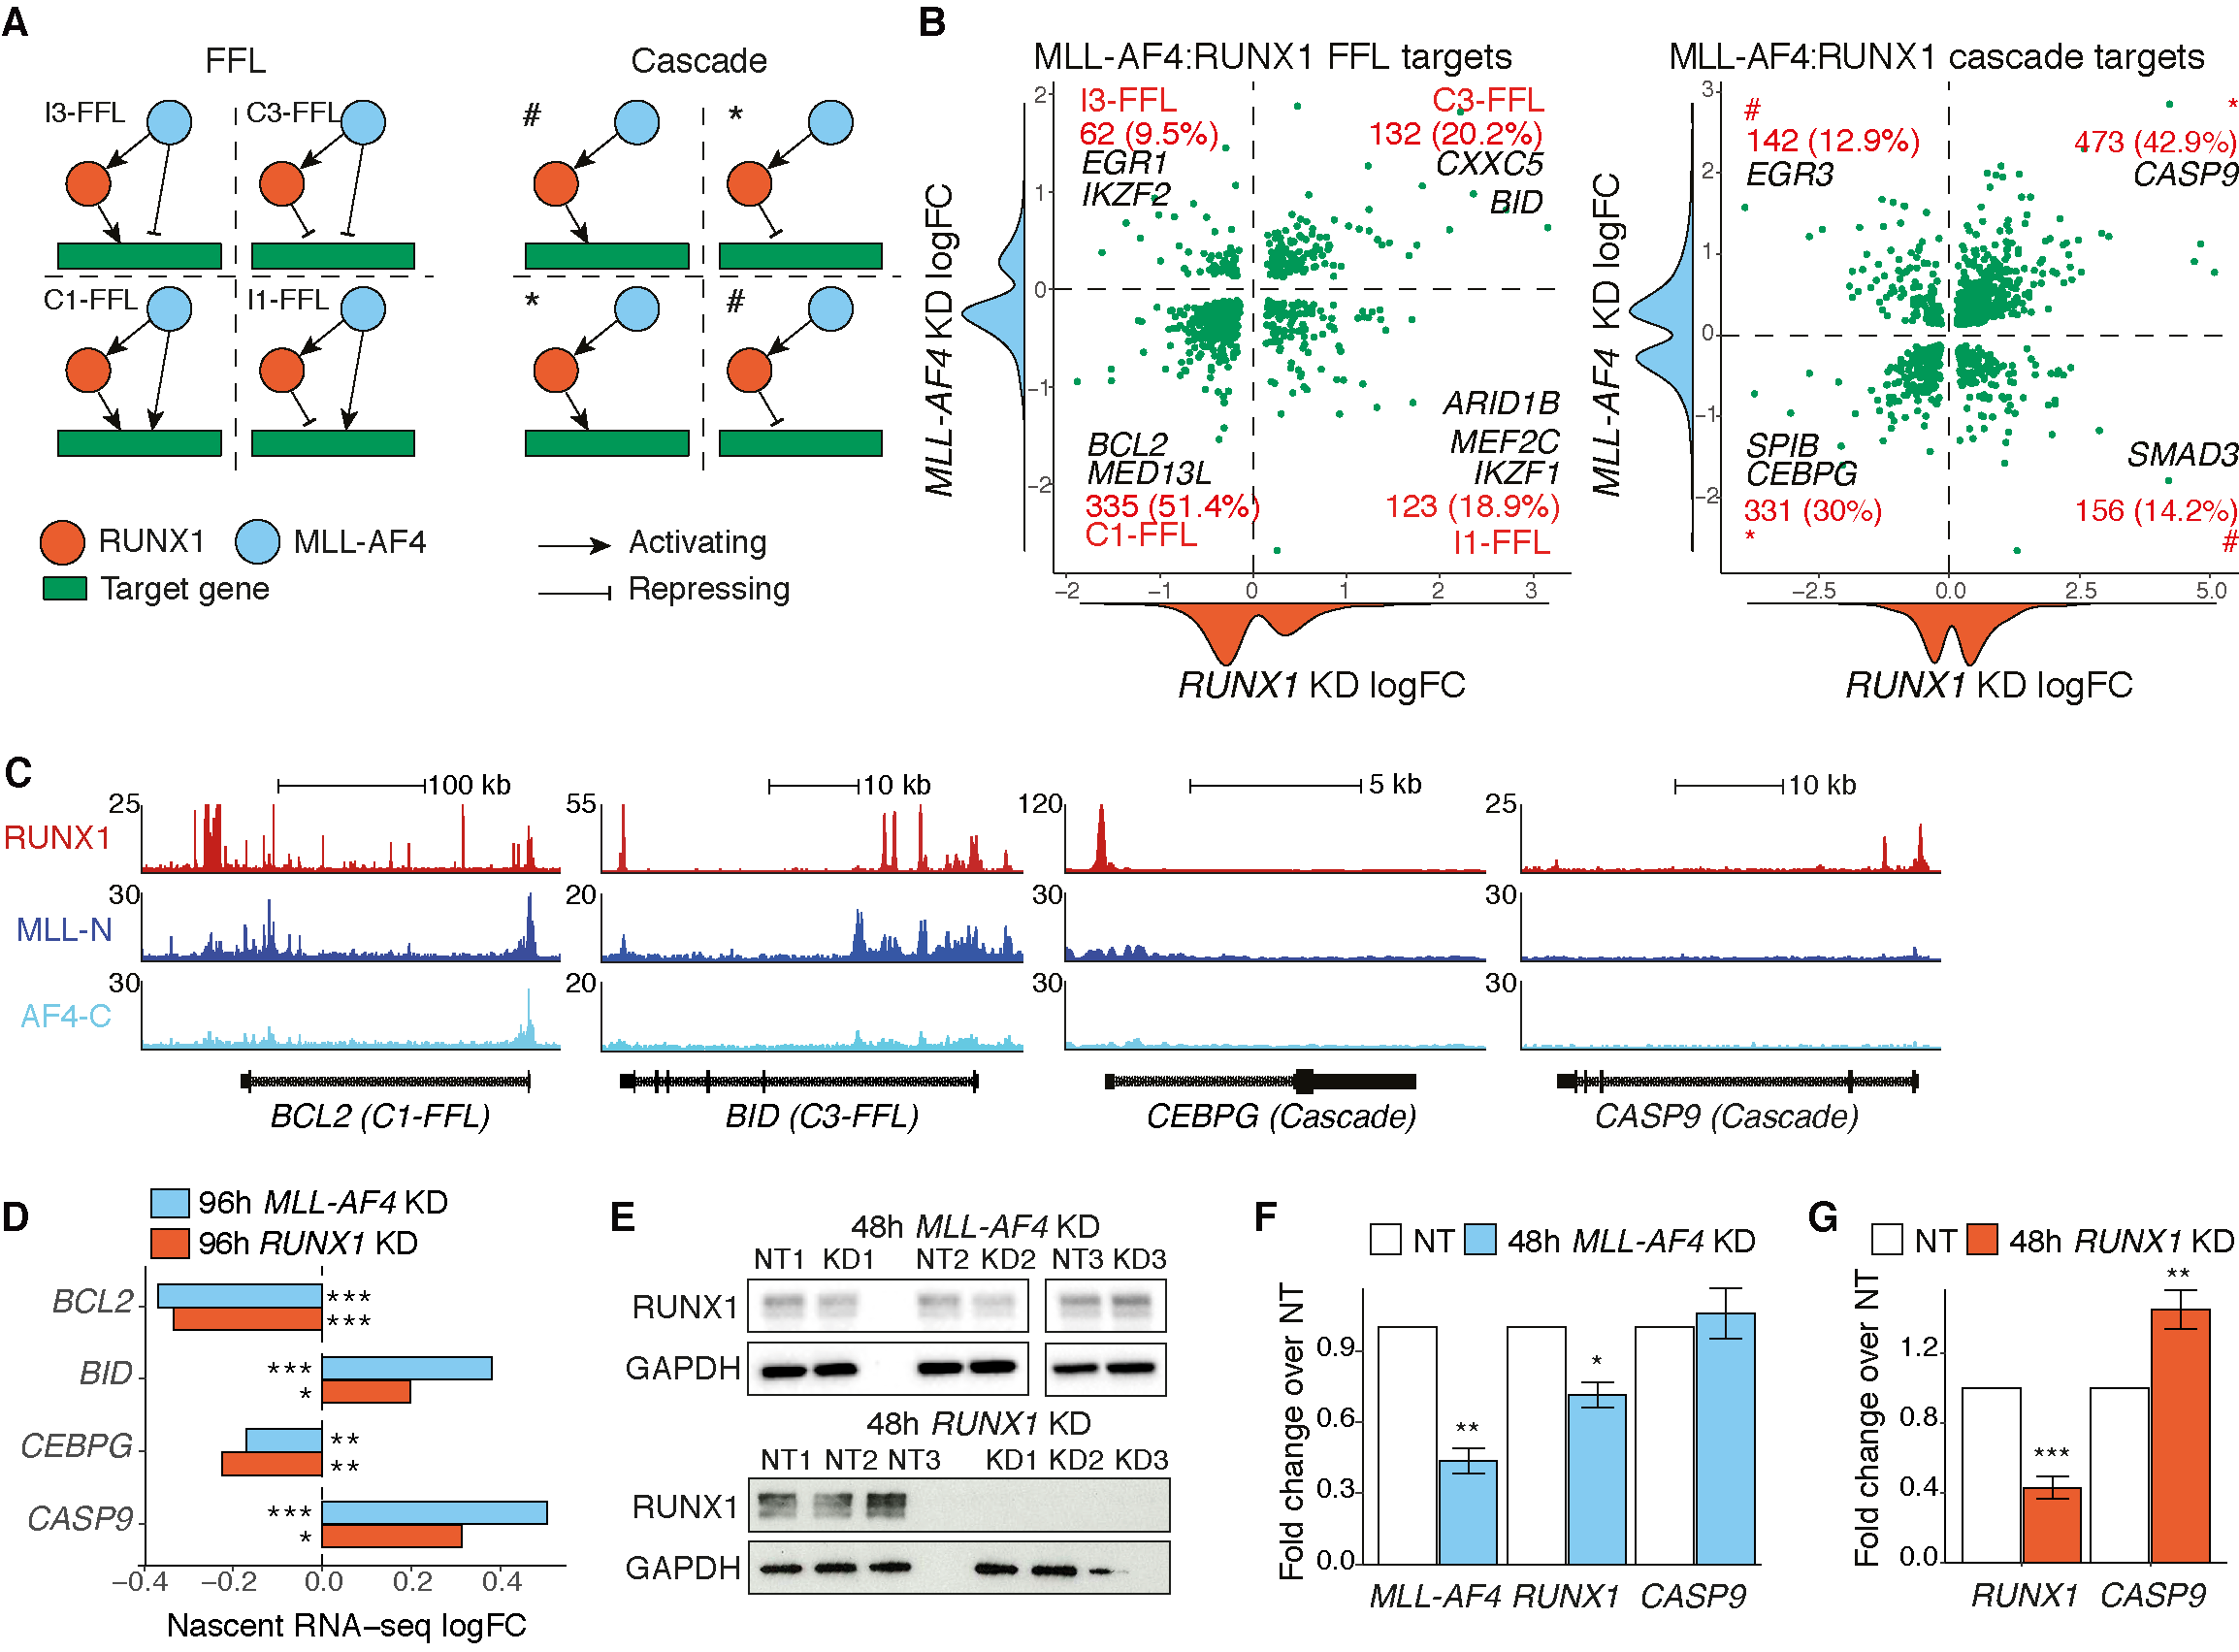
\includegraphics[width=\textwidth,height=\textheight,keepaspectratio]{figures/chapter4/chr4_grn-motifs.png}
    %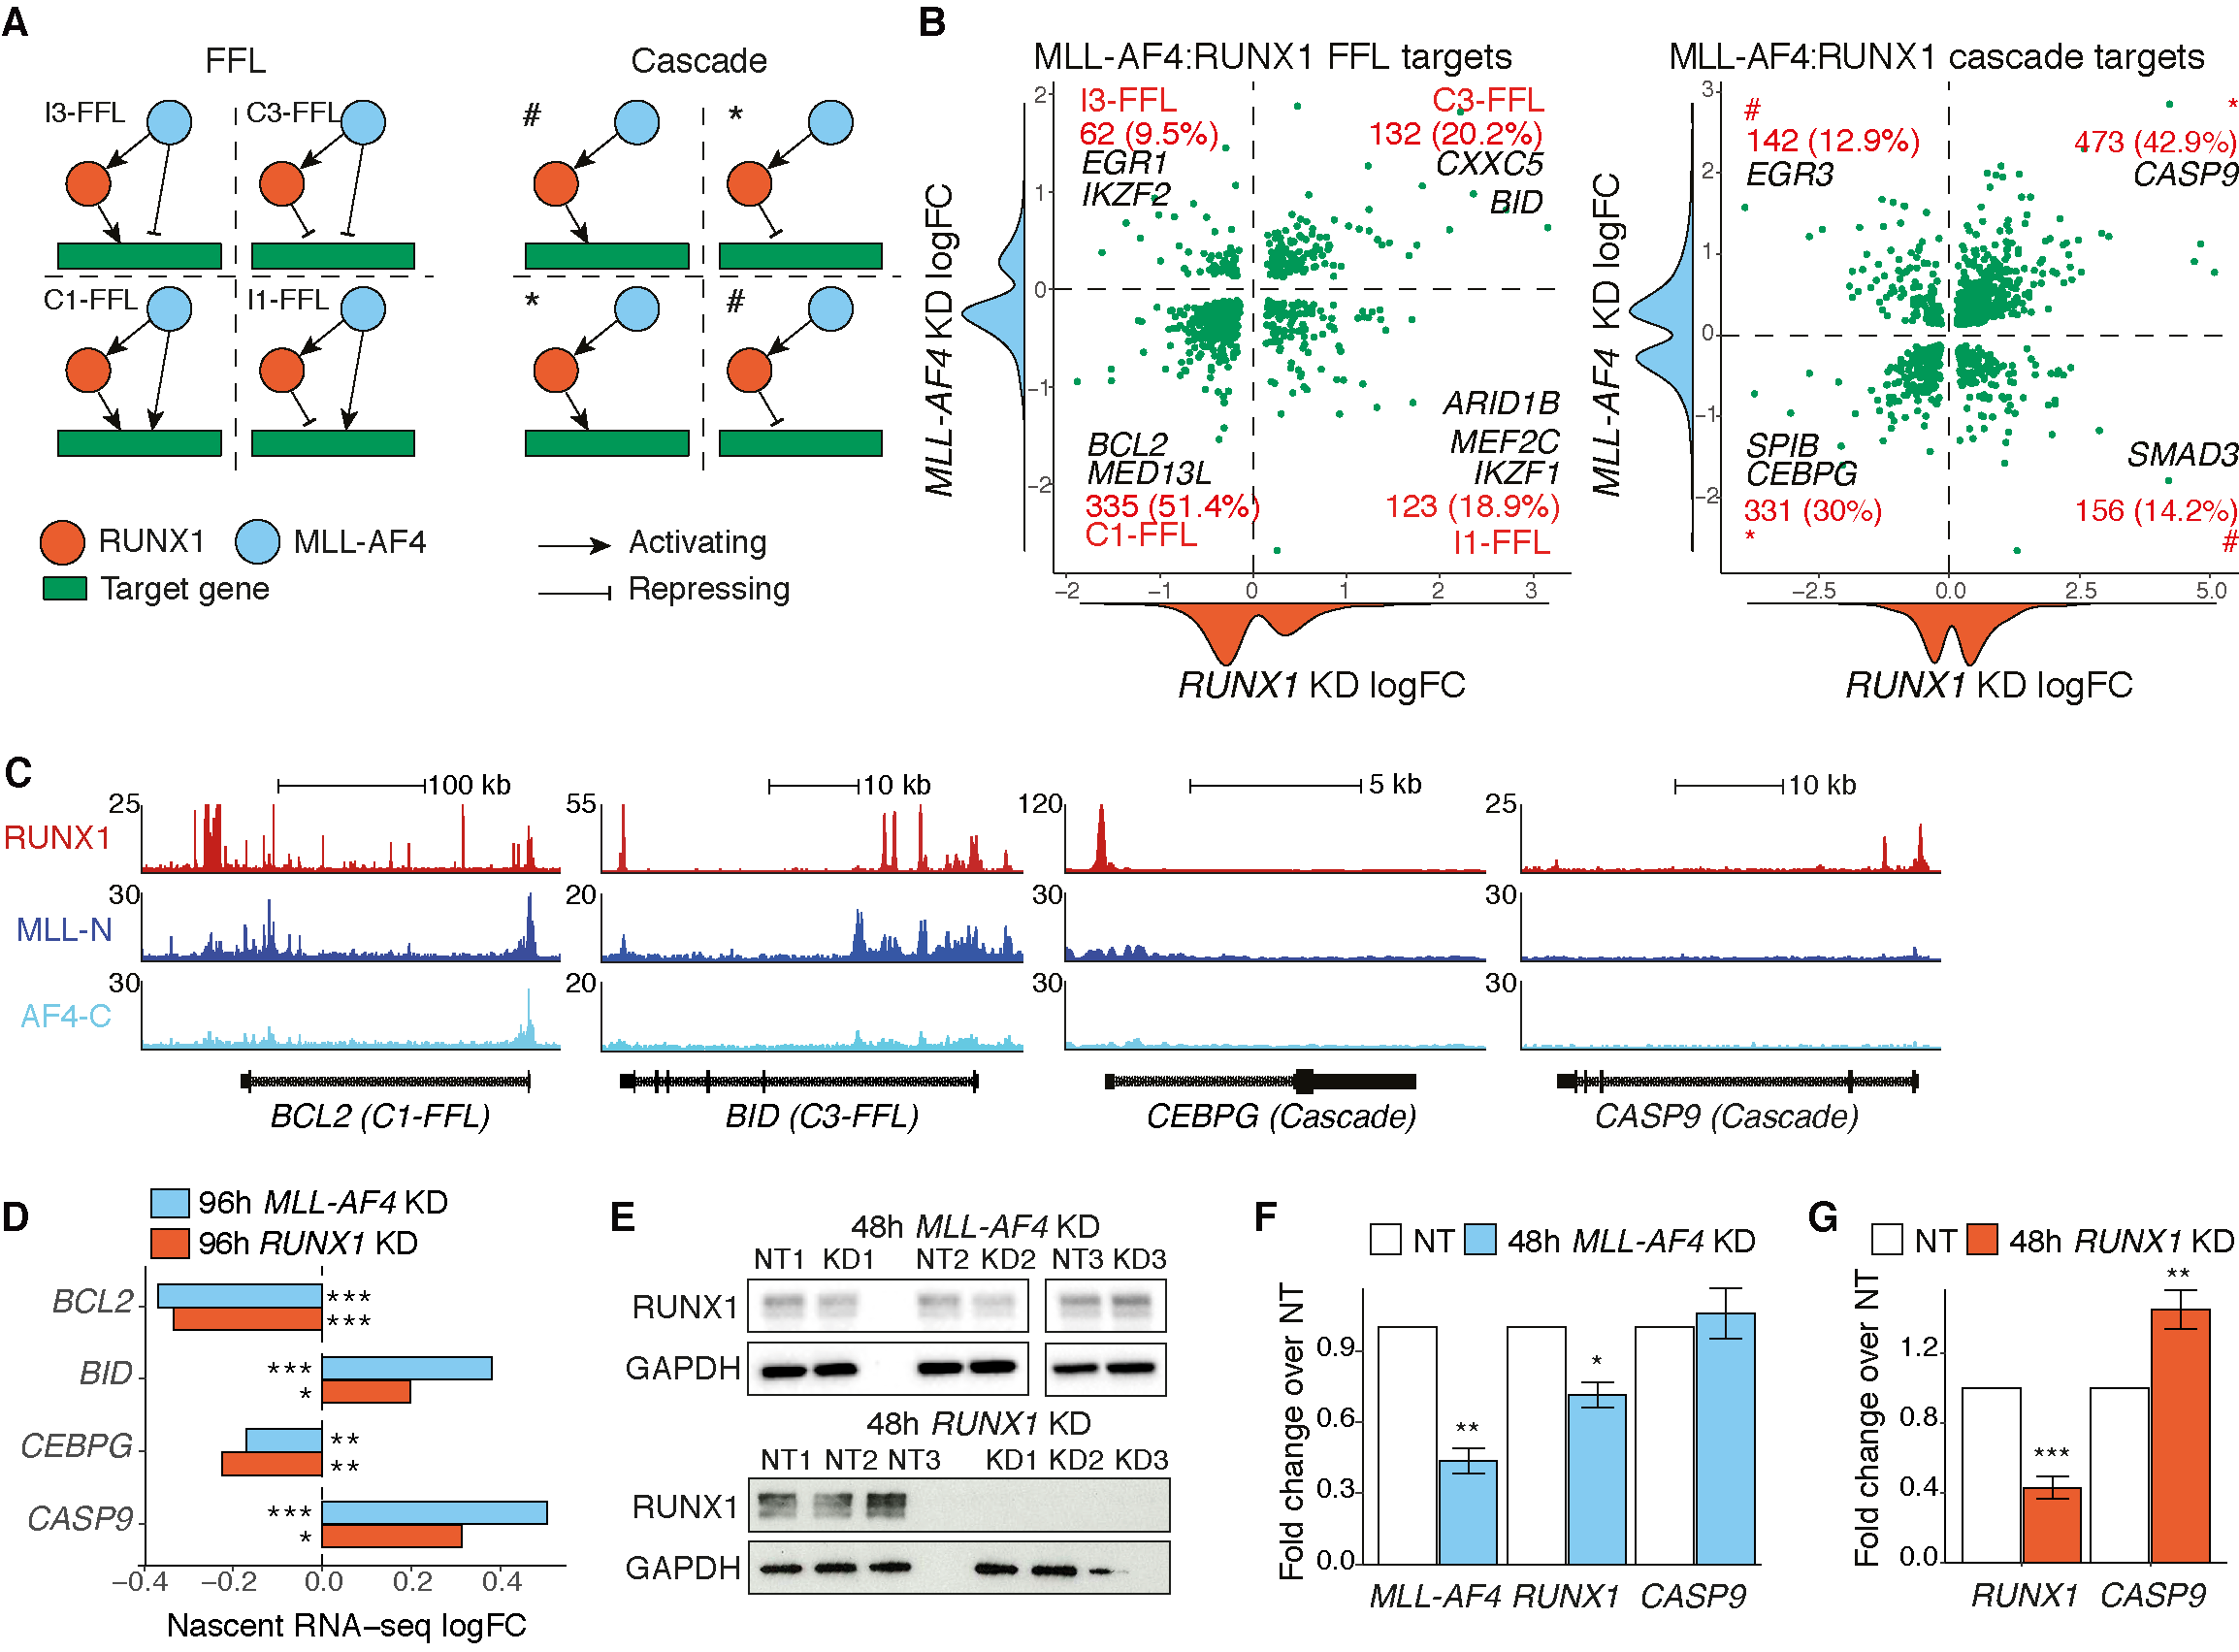
\includegraphics{figures/chapter4/chr4_grn-motifs.png}
    \caption[{Network motifs describing interplay between RUNX1 and MLL-AF4.}]
    {\textbf{Network motifs describing interplay between RUNX1 and MLL-AF4.} 
    \textbf{(A)} Illustration of FFL sub-types (left) and cascade (right) motifs. *: Same sign of effect. \#: Opposing sign of effect.
    \textbf{(B)} LogFC response to \textit{RUNX1} and \textit{MLL-AF4} KD in FFL (left) and TF cascade (right) target genes. Density plots of logFC distribution along axis. Quadrants of scatter plots align with FFL and cascade subtypes shown in A.
    \textbf{(C)} ChIP-seq tracks for MLL-N, AF4-C, and RUNX1 at \textit{BCL2} (C1-FFL target), \textit{BID} (C3-FFL target), \textit{CEBPG} and \textit{CASP9} (cascade targets). 
    \textbf{(D)} Nascent RNA-seq logFC following 96h \textit{RUNX1} or \textit{MLL-AF4} KD.
    \textbf{(E)} Western blot for RUNX1 protein in SEM cells after 48 h \textit{MLL-AF4} KD or 48 h \textit{RUNX1} KD, with GAPDH as loading control. 
    \textbf{(F, G)} qRT-PCR assaying \textit{MLL-AF4}, \textit{RUNX1} and \textit{CASP9} expression following 48 h \textit{MLL-AF4} KD (F) or 48 h \textit{RUNX1} KD (G) in SEM cells (\textit{n} = 3). 
    (*) P < 0.05; (**) P < 0.01; (***) P < 0.001
    \textit{Adapted from \cite{harman_kmt2a-aff1_2021}.}
    }
    \label{fig:ch4_motifs}
\end{figure}

While MLL-AF4 and RUNX1 regulatory logic intersects at key pathways, it is yet unclear whether these factors cooperate directly, or if this intersection is driven through RUNX1 acting as an intermediate TF. To dissect how RUNX1 and MLL-AF4 co-regulate gene targets I integrated the GRN models, then identified FFL and TF cascade regulatory motifs. Regulatory logic was predicted using the siRNA perturbation data (Fig. \ref{fig:ch4_GRN_just}A, Fig. \ref{fig:ch4_runx1-grn}A-B), where loss of gene expression upon KD implies positive regulation, and vice versa. This method assumes expression responses are a direct result of MLL-AF4 or RUNX1 regulation. It is well established that MLL-AF4 drives \textit{RUNX1} overexpression \citep{wilkinson_runx1_2013}, so this constrains possible FFL subtypes into just four categories. These include two coherent (C1- and C3-FFL) and two incoherent FFLs (I1- and I3-FFL), with subtypes classified by MLL-AF4 and RUNX1 regulation of genes \citep{mangan_structure_2003} (Fig. \ref{fig:ch4_motifs}A). Cascade motifs were identified as genes directly regulated by RUNX1, but indirectly (i.e., not bound) by MLL-AF4. These were further classified into so-called "coherent" and "incoherent" groups (Fig. \ref{fig:ch4_motifs}A, coherent and incoherent denoted by * and \# respectively). Coherent cascades show an alignment between the effect of \textit{RUNX1} and \textit{MLL-AF4} KD, which agrees with the hypothesis that RUNX1 targets a wider network as an intermediate for MLL-AF4.

Overall, we found that 71.6\% of FFLs were coherent, suggesting that MLL-AF4 and RUNX1 act cooperatively at the same loci (Fig. \ref{fig:ch4_motifs}B). For example, the key MLL-AF4 target \textit{BCL2} is activated in a C1-FFL, while \textit{BID} is repressed in a C3-FFL, with both loci bound by MLL-AF4 and RUNX1 (Fig. \ref{fig:ch4_motifs}C-D). FFL subtypes are typically biased towards a C1-FFL configuration \citep{joanito_incoherent_2018, mangan_incoherent_2006}, which is recapitulated in our analysis, with 51.5\% of FFLs showing cooperative activation of target genes (Fig. \ref{fig:ch4_motifs}B), further suggesting that RUNX1 at these FFL sites is biased towards activation. Interestingly, the EHT Runx1 target \textit{Ikzf1} (Fig. \ref{fig:ch3_pairwise}, p.\pageref{fig:ch3_pairwise}) is targeted in an I1-FFL in the MLL-AF4 GRN, where RUNX1 appears to repress \textit{IKZF1} rather than activate (RUNX1 KD logFC: 0.93, FDR: 2.8 x 10\textsuperscript{-43}), despite similar RUNX1 binding profiles to EHT (Fig. \ref{fig:ch4_runx1-grn}D). This change in RUNX1 regulation could be due to the leukaemic or the B cell context, in the presence of different cofactors and TFs.

The majority of cascade motifs are "coherent" (72.9\%, Fig. \ref{fig:ch4_motifs}B), suggesting that RUNX1 is a strong determining factor for regulation at the majority of cascade motifs. Example cascade targets are \textit{CEBPG} (activated) and \textit{CASP9} (repressed), where RUNX1 is bound but MLL-AF4 is not (Fig. \ref{fig:ch4_motifs}C-D). Incoherent cascades (27.1\%, Fig. \ref{fig:ch4_motifs}B) are likely a result of noise in the nascent RNA-seq experiments or regulatory control by additional TFs. Interestingly, while FFLs show a strong activation bias, cascade motifs are balanced between activating and repressive. This suggests that while RUNX1 behaves as an activator when at the same genes as MLL-AF4, at other sites RUNX1 may act as either an activator or a repressor. This is consistent with dual RUNX1 activity in haematopoietic differentiation \citep{kuvardina_runx1_2015, lutterbach_role_2000, canon_vivo_2003}.

The repressed cascade target \textit{CASP9} (caspase-9) was validated by performing siRNA KD for a shorter length of time. To generate the GRN, \textit{MLL-AF4} and \textit{RUNX1} KDs were performed for 96 hours to achieve a robust reduction in protein, resulting in significant \textit{CASP9} upregulation (Fig. \ref{fig:ch4_motifs}D); however, this timepoint also favours secondary effects. A shorter-term \textit{MLL-AF4} KD for 48 hours reduces \textit{RUNX1} mRNA levels, but does not impact RUNX1 protein, and has little effect on \textit{CASP9} expression (P = 0.64, Fig. \ref{fig:ch4_motifs}E-F), consistent with indirect regulation of \textit{CASP9} by MLL-AF4. \textit{CASP9} is upregulated with just 48 hours' \textit{RUNX1} KD, as with 96 hours' KD, suggesting that RUNX1 may directly repress the gene (Fig. \ref{fig:ch4_motifs}E, G). As \textit{CASP9} is sensitive to \textit{RUNX1} perturbation at an earlier timepoint, but not with \textit{MLL-AF4}, this confirms that MLL-AF4 may act in this TF cascade through RUNX1 activity.

\begin{figure}[t]
    \centering
    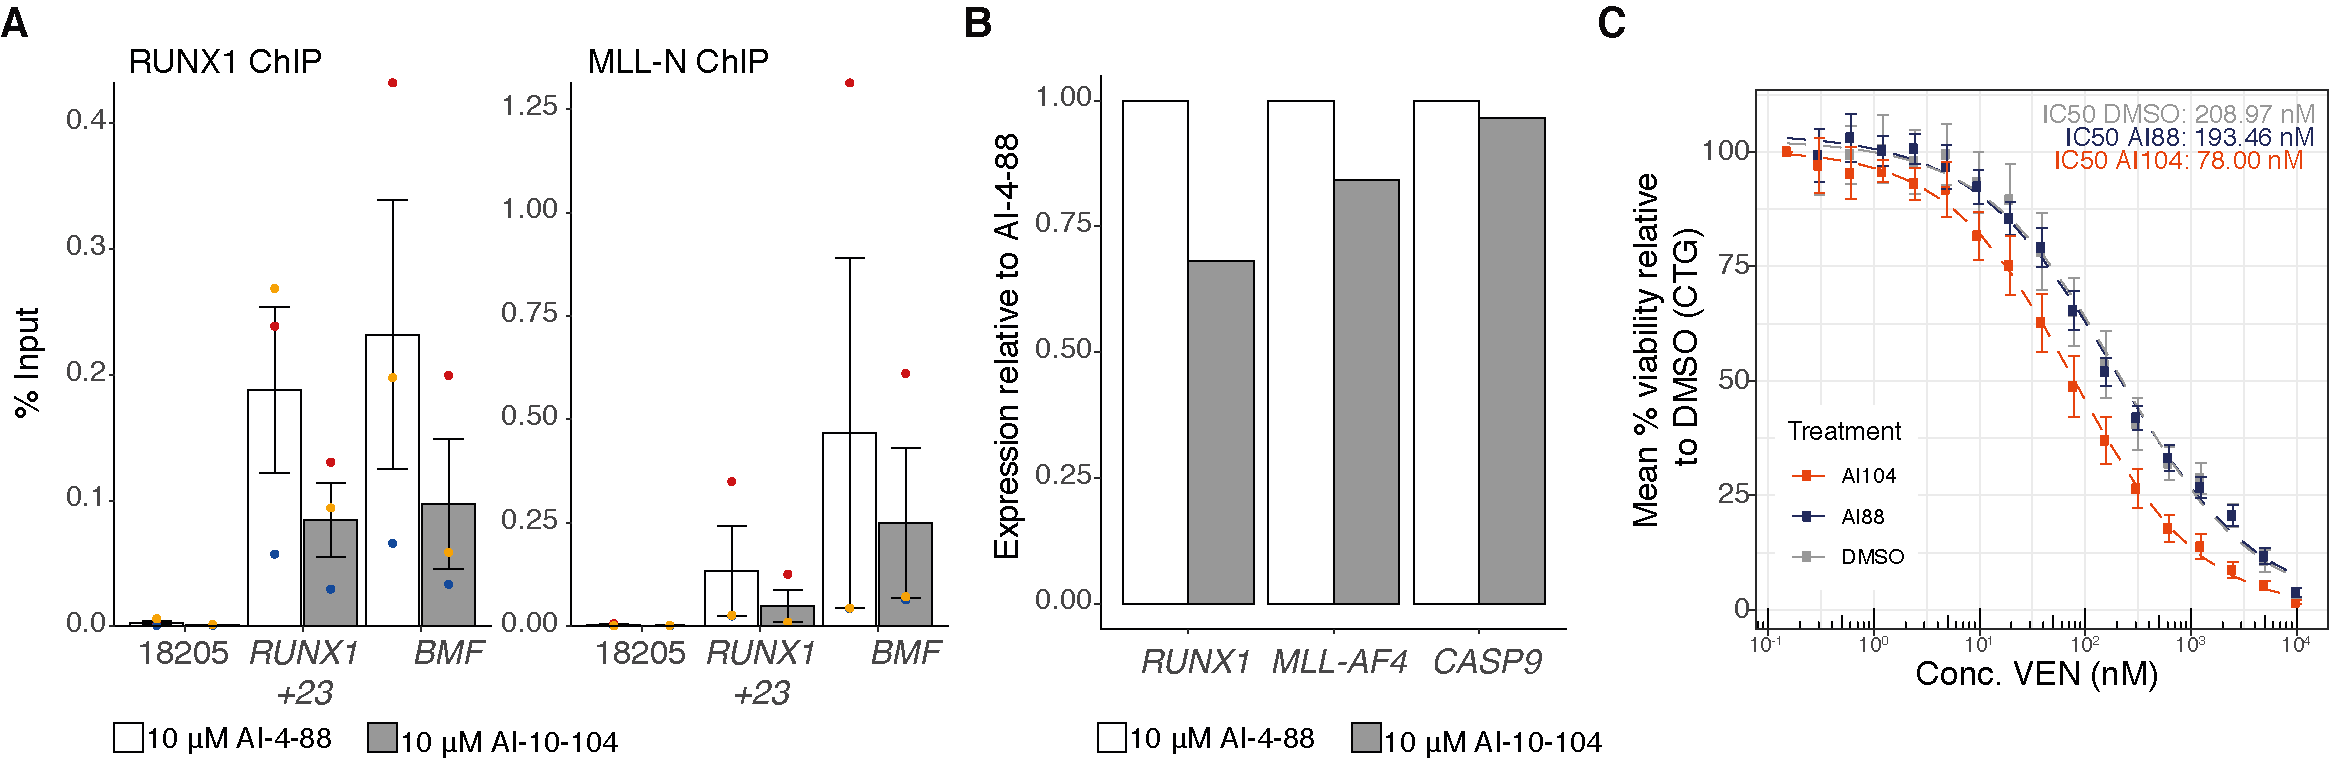
\includegraphics[width=\textwidth,height=\textheight,keepaspectratio]{figures/chapter4/chr4_runx1-inh.png}
    %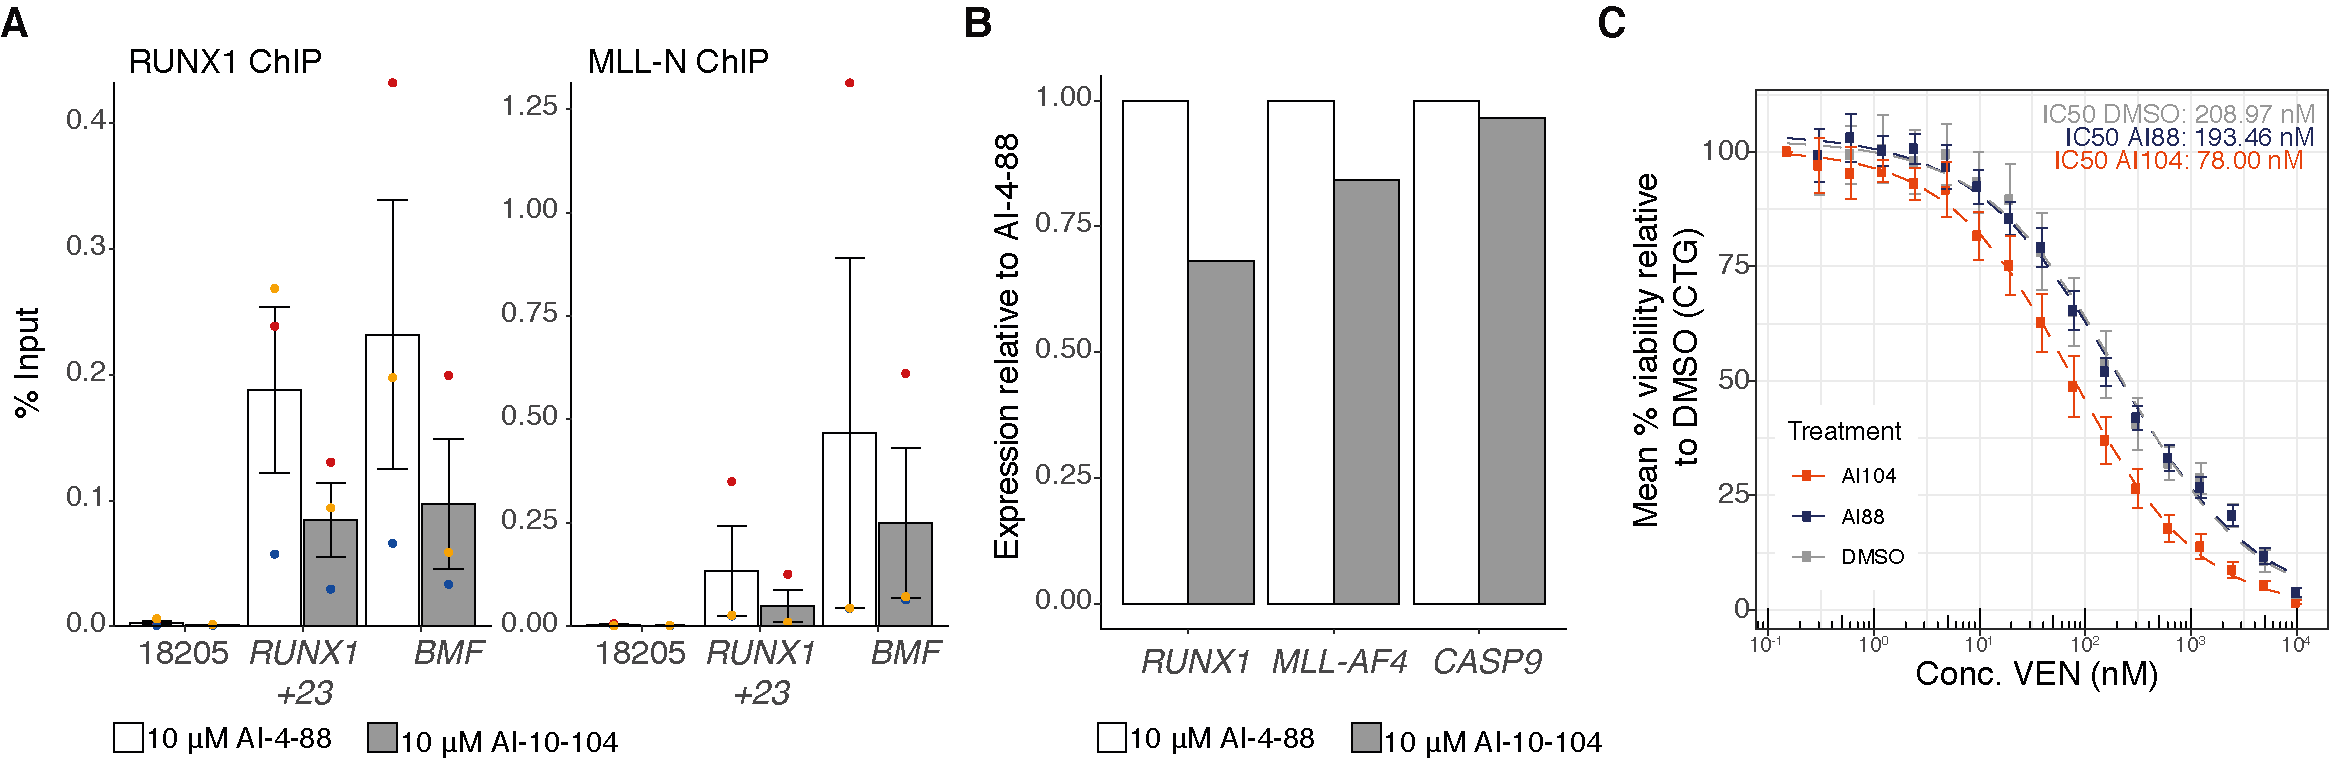
\includegraphics{figures/chapter4/chr4_runx1-inh.png}
    \caption[{RUNX1 inhibitor treatment reduces the IC50 concentration of venetoclax.}]
    {\textbf{RUNX1 inhibitor treatment reduces the IC50 concentration of venetoclax.} 
    \textbf{(A)} RUNX1 and MLL-N ChIP-qPCR after 24 h 10 \microm{} AI-10-104 or AI-4-88 (inactive control) treatment (as used in SEM cells in \cite{illendula_small_2016}), normalised to input chromatin. Regions probed are the \textit{RUNX1} +23 enhancer and a RUNX1 bound peak at the \textit{BMF} locus. 18205 refers to a negative control locus. Bars show mean, and error bars represent SEM (\textit{n} = 3).
    \textbf{(B)} qRT-PCR analysis showing \textit{RUNX1}, \textit{MLL-AF4}, and \textit{CASP9} expression after 24 h 10 \microm{} AI-10-104 or AI-4-88 (inactive control) treatment (\textit{n} = 1). Expression normalised to \textit{GAPDH} shown relative to AI-4-88.
    \textbf{(C)} Dose response curve of SEM cells treated with venetoclax for 24 h. Cells were co-treated with 10 \microm{} AI-10-104, AI-4-88 or DMSO). Viability measured using CTG, normalised to DMSO control. Dashed line represents dose response curve fit, and IC50 was calculated in the context of RUNX1 inhibitors. (\textit{n} = 8). 
    }
    \label{fig:ch4_runx1-inh}
\end{figure}

In publishing this data, in collaboration with M. Jamilly (Fulga lab), the MLL-AF4:RUNX1:\textit{CASP9} TF cascade was implicated as a potential promoter of venetoclax resistance \citep{harman_kmt2a-aff1_2021}. Venetoclax is a BCL2 inhibitor that is used to treat \textit{MLL}r leukaemia \citep{khaw_venetoclax_2016, vandenberg_abt-199_2013}, though drug resistance is a concern. As caspase-9 lies downstream of BCL2 in the apoptotic pathway, the MLL-AF4:RUNX1:\textit{CASP9} cascade may provide a potential circuit for deterring apoptosis. To test whether RUNX1 activity interacts with venetoclax efficacy, I treated SEM cells with a small molecule RUNX1 inhibitor (active AI-10-104, inactive AI-4-88) that disrupts RUNX1 binding to the TF CBF$\beta$ \citep{illendula_small-molecule_2015, illendula_small_2016}, resulting in reduced RUNX1 DNA binding and expression (Fig. \ref{fig:ch4_runx1-inh}A-B). This reduced \textit{RUNX1} expression is likely due to loss of positive RUNX1 autoregulation \citep{martinez_transcriptional_2016}. I generated venetoclax dose-response curves, and co-treated with 10 \microm{} RUNX1 inhibitor. Co-treatment with AI-10-104 yielded a lower venetoclax IC50 (78 nM) over AI-4-88 or DMSO treatment (208.97 nM, 193.47 nM) (Fig. \ref{fig:ch4_runx1-inh}C). This preliminary analysis suggests an interaction between venetoclax and RUNX1 activity, though \textit{CASP9} levels appear unaffected by RUNX1 inhibition, so it is possible that this effect is mediated through alternative pathways (Fig. \ref{fig:ch4_runx1-inh}B). Additional replicates are needed to determine \textit{CASP9} sensitivity to AI-10-104 treatment. Recent studies have noted improved venetoclax response in patients with \textit{RUNX1} mutations, and have suggested this effect is through generally reducing the apoptotic threshold \citep{cherry_venetoclax_2021, chow_runx1_2021}. A more robust experimental design is required to determine if the effect is synergistic.

\subsection[Correlation between MLL-AF4 and RUNX1 ChIP-seq binding profiles]{\label{ch4:ma4-runx1-cor}Correlation between MLL-AF4 and RUNX1\\ChIP-seq binding profiles}

The number of MLL-AF4:RUNX1 FFLs and the shared regulatory logic at these genes suggests a synergistic interaction between the two factors. To investigate this possibility, I performed correlative analyses of genome wide chromatin binding profiles. For the TFs analysed (RUNX1 and MAZ), there was reasonable correlation with MLL-N ChIP-seq signal at promoters (Fig. \ref{fig:ch4_ma4-TF-cor}A), and genome wide binding patterns show general co-localisation of the TFs and MLL-N (Fig. \ref{fig:ch4_ma4-TF-cor}B). MLL-AF4 binding is broader than TFs peaks, and MLL-FP spreading is associated with highly overexpressed targets \citep{kerry_mll-af4_2017} (Fig. \ref{fig:ch4_ma4-TF-cor}A), making precise comparisons between MLL-AF4 and TFs difficult. However, with increased MLL-AF4 spreading I observed a similar spread of TF binding, with an increased number of TF peaks. This is exemplified at \textit{GNAQ}, where rather than typical spreading, a higher frequency of TF binding can be seen co-localising with MLL-AF4 spreading (Fig. \ref{fig:ch4_ma4-TF-cor}A).

\begin{figure}[htbp]
    \centering
    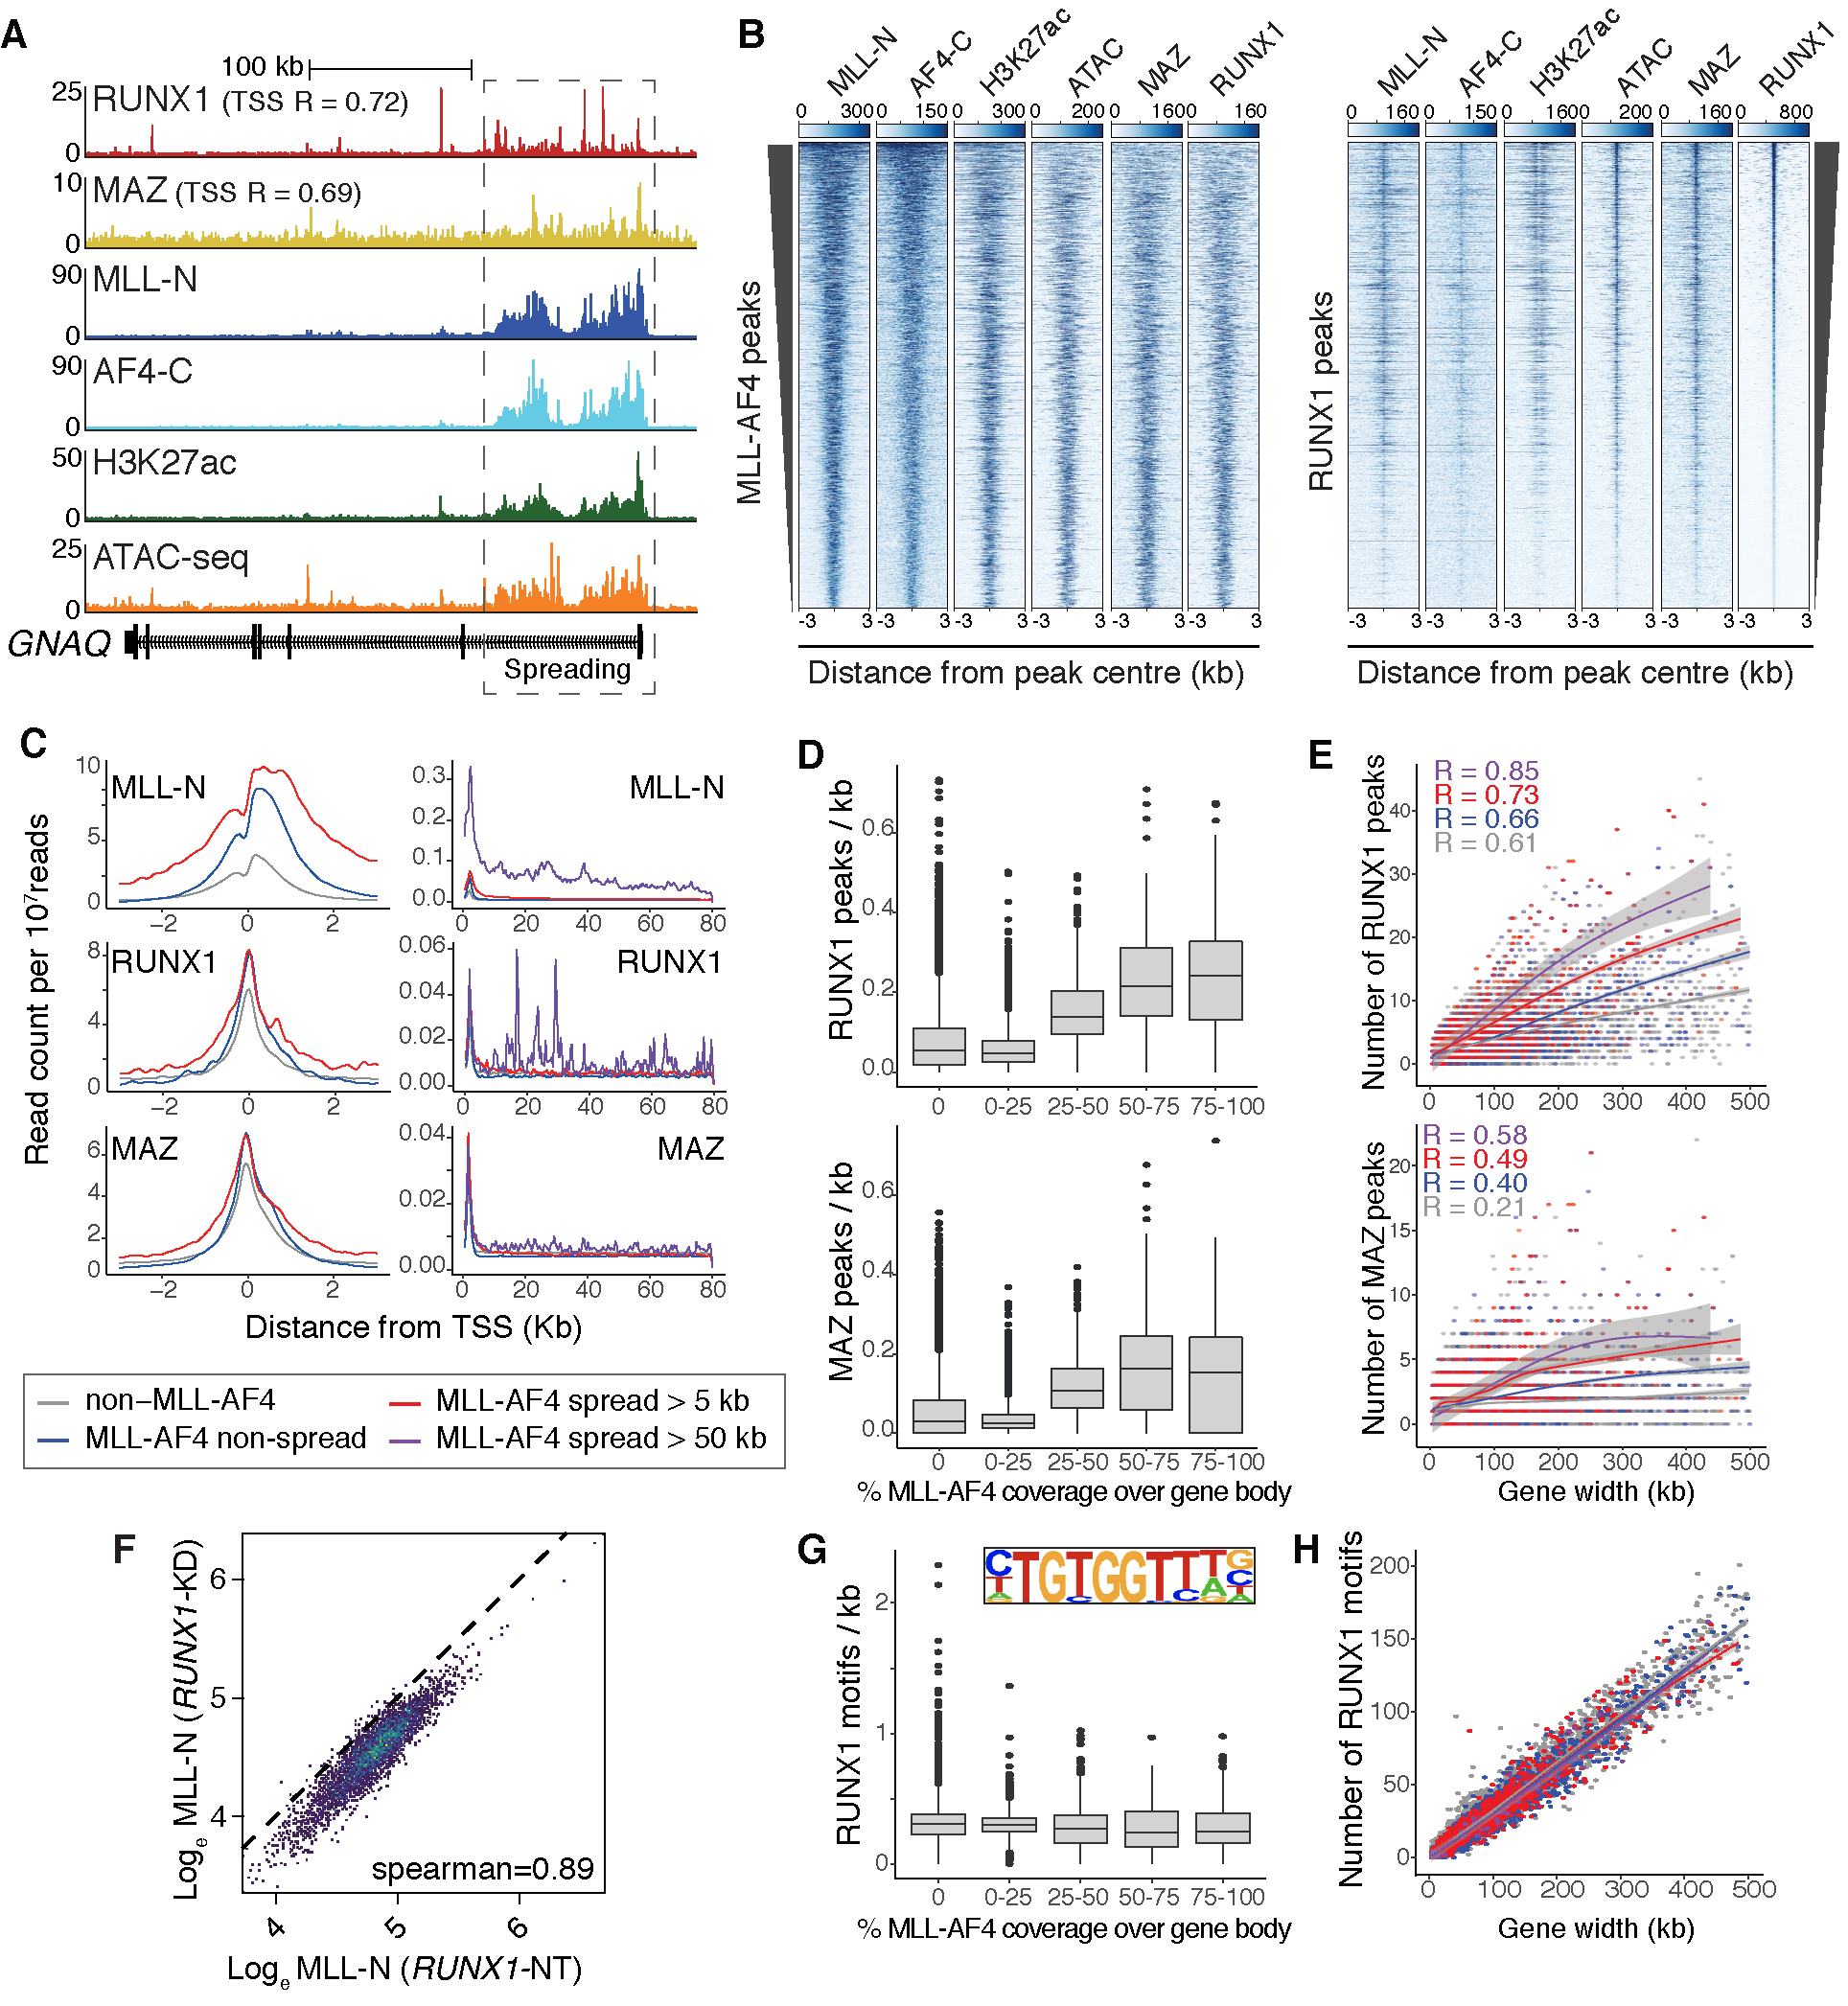
\includegraphics[width=\textwidth,height=\textheight,keepaspectratio]{figures/chapter4/chr4_ma4-TF-correlation.png}
    %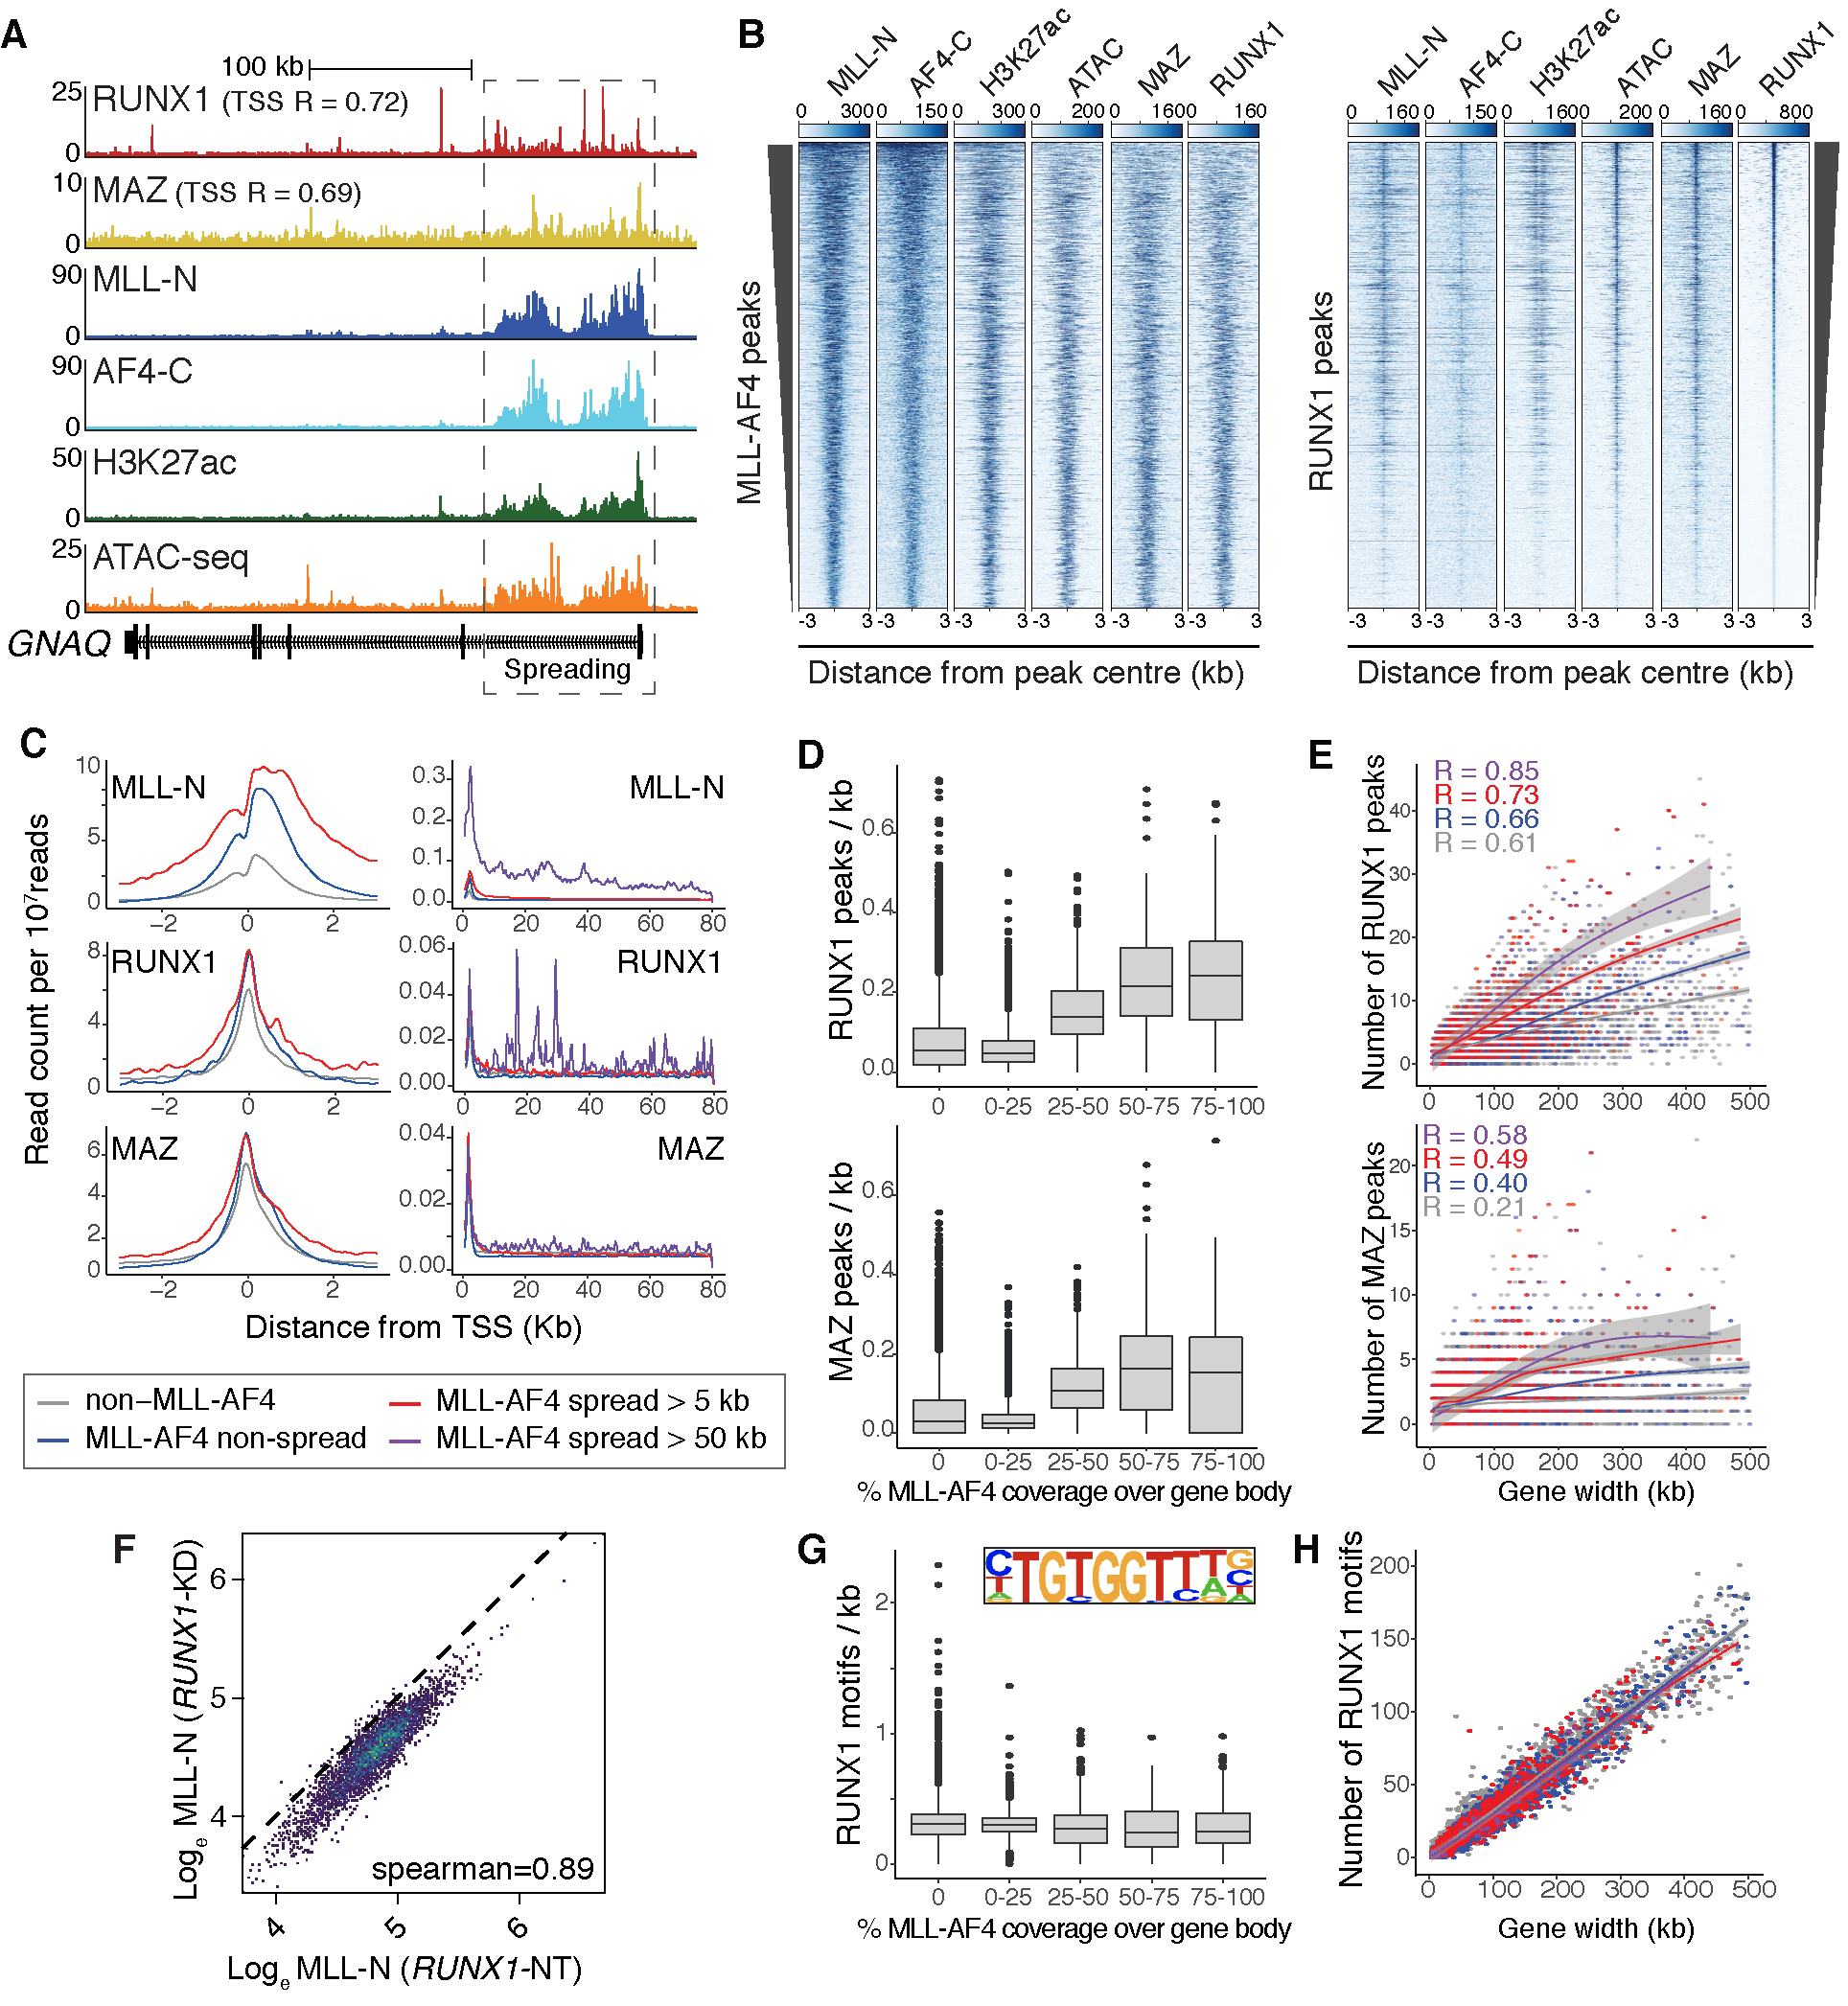
\includegraphics{figures/chapter4/chr4_ma4-TF-correlation.png}
    \caption[{MLL-AF4 establishes an environment encouraging TF binding and FFL formation.}]
    {\textbf{MLL-AF4 establishes an environment encouraging TF binding and FFL formation.} 
    \textbf{(A)} ChIP-seq tracks for GRN TFs, H3K27ac and ATAC-seq at \textit{GNAQ}. Correlation (\textit{R}) comparing TF ChIP-seq signal with MLL-N over expressed gene promoters. Dashed box highlights MLL-AF4 spreading.
    \textbf{(B)} ChIP-seq and ATAC-seq heatmaps in SEM cells, at MLL-AF4 peaks (left) and RUNX1 peaks (right), ordered by ChIP-seq signal.
    \textbf{(C)} Mean ChIP-seq signal at expressed promoters over a 6 kb (left) or 80 kb (right) window. Profiles stratified by MLL-AF4 binding classes as labelled.
    \textbf{(D,G)} TF ChIP-seq peaks/kb (D) or RUNX1 motifs/kb (G) over gene bodies, stratified by proportion of MLL-AF4 coverage.
    \textbf{(E,H)} Relationship between TF peak (E) or RUNX1 motif (H) frequency over gene bodies, and gene body length (kb), stratified by MLL-AF4 binding classes as in C. Local regression (LOESS) lines fit with 95\% CI in grey. Correlation (\textit{R}) calculated by MLL-AF4 binding classes. RUNX1 motif logo shown.
    \textbf{(F)} Log\textsubscript{e} MLL-N ChIP-seq reads at MLL-AF4 peaks following 48 hours’ treatment with NT or RUNX1 siRNA. 
    }
    \label{fig:ch4_ma4-TF-cor}
\end{figure}

To test whether increased TF binding is associated with MLL-AF4 genome wide, I analysed TF peak densities at gene loci. I first classified expressed genes by MLL-AF4 spreading status, differentiating between > 5 kb spreading (754 genes) and > 50 kb spreading (25 genes). TF binding at promoters was more intense at all MLL-AF4 targets over non-MLL-AF4, and showed increased signal outside the promoter at spreading targets. Further, with > 50 kb spreading there was increased TF signal over 50 kb away from gene promoters (Fig. \ref{fig:ch4_ma4-TF-cor}C). The density of TF ChIP-seq peaks across a gene body (peaks/kb) increased with a greater proportion of MLL-AF4 coverage (Fig. \ref{fig:ch4_ma4-TF-cor}D). The relationship between total TF peaks and gene body length is also stronger at MLL-AF4 spreading targets over non-spreading or unbound genes (Fig. \ref{fig:ch4_ma4-TF-cor}E). The TF peak density at spreading targets is much higher with RUNX1 than MAZ, though the relationship is present in both cases. Together this suggests that with a greater spread of MLL-AF4 there is an increased frequency of TF binding. 

As this analysis is correlative, whether TF binding encourages MLL-AF4 spreading or MLL-AF4 drives TF binding remains unclear. To determine whether TFs may influence MLL-AF4 binding or spreading patterns I first performed \textit{RUNX1} siRNA KD. With 48 hours' \textit{RUNX1} KD MLL-AF4 binding genome wide is slightly reduced, though profiles are largely maintained with no site-specific loss of MLL-AF4 and high correlation between KD and control samples (Fig. \ref{fig:ch4_ma4-TF-cor}F). The slight reduction in MLL-AF4 binding could reflect a subtle impact on MLL-AF4 protein levels, though nascent \textit{MLL-AF4} expression is unaffected (96h \textit{RUNX1} KD RNA-seq: logFC = 0.1, FDR = 0.12). It remains difficult to disentangle the effect of \textit{MLL-AF4} perturbation on RUNX1 binding, as MLL-AF4 directly drives \textit{RUNX1} expression. Therefore, I cannot confidently conclude that MLL-AF4 directs TF binding, though the correlation is suggestive. Importantly, while RUNX1 binding frequency increases with MLL-AF4 spreading, RUNX1 motifs do not (Fig. \ref{fig:ch4_ma4-TF-cor}G-H). This could imply the increased TF binding is through non-sequence specific DNA binding mechanisms, such as association with larger protein complexes, or that RUNX1 motifs are in equal excess across genes and MLL-AF4 establishes increased RUNX1 motif binding affinity. This analysis suggests that MLL-AF4 and TFs co-localise to form FFL circuits, in a process that may be driven by MLL-AF4. An attractive hypothesis is that MLL-AF4 increases the binding affinity of TFs for existing motifs, through epigenetic modification and increased chromatin accessibility.

\section{\label{ch4:tf-cointeraction}TF cooperation at MLL-AF4 targets drives expression and promotes leukaemogenesis}

The data presented thus far offer a breakdown of MLL-AF4 and TF cooperation in FFLs, and indirect MLL-AF4 regulation using TFs as intermediates in cascade motifs. FFL motifs are particularly prominent, and there appears to be a relationship between MLL-AF4 and TF binding, promoting co-localisation at MLL-AF4 target sites. As MLL-AF4 and RUNX1 networks intersect at regulation of cell death and cell cycle processes (Fig. \ref{fig:ch4_interplay}B), it is likely that RUNX1 drives regulation of these processes. Key genes that regulate proliferation and apoptosis include \textit{MYC} \citep{dang_myc_2012} and \textit{BCL2} \citep{kale_bcl-2_2018}. MLL-AF4 regulates both of these factors \citep{robinson_abundant_2008, benito_mll-rearranged_2015}, and as MLL-AF4 appears to increase TF binding affinity (Fig. \ref{fig:ch4_motifs} and Fig. \ref{fig:ch4_ma4-TF-cor}), the overexpression of these genes may be partly driven by cooperative TF activity. I therefore investigated whether RUNX1 co-interacts with other TFs to drive \textit{BCL2} and \textit{MYC} expression.

\begin{figure}[t]
    \centering
    \includegraphics[width=\textwidth,height=\textheight,keepaspectratio]{figures/chapter4/ch4_tf-coop.png}
    %\includegraphics{figures/chapter4/ch4_tf-coop.png}
    \caption[{GRN predicted cooperative regulation of \textit{MYC} and \textit{BCL2}.}]
    {\textbf{GRN predicted cooperative regulation of \textit{MYC} and \textit{BCL2}.} 
    \textbf{(A)} Frequency of TFs co-regulating gene targets with RUNX1. Core MLL-FP TFs highlighted in red. 
    \textbf{(B, C)}  Sub-networks of select interactions from MLL-AF4 and TFs regulating \textit{MYC} (B) and \textit{BCL2} (C). 
    \textbf{(D)} ChIP-seq tracks for MAZ, MYB, RUNX1 and MLL-N at \textit{MYC} and its super enhancer (1.7 Mb downstream of promoter), and \textit{BCL2} and its enhancer (218 kb downstream of promoter). 
    \textbf{(E)} qRT-PCR analysis probing \textit{BCL2} pre-mRNA after 48 h siRNA treatment (\textit{n} = 3). Expression normalized to \textit{GAPDH}, and shown relative to NT control. 
    Bars show mean with standard error; (*) P < 0.05; (**) P < 0.01.
    \textit{Adapted from \cite{harman_kmt2a-aff1_2021}. Myb ChIP-seq data sourced from \citep{godfrey_dot1l_2019}.}
    }
    \label{fig:ch4_tf-coop}
\end{figure}

The most frequent TFs to co-regulate the same genes as RUNX1 include core MLL-FP GRN TFs NF-YA, MYB, IKZF1 and MEF2C (Fig. \ref{fig:ch4_tf-coop}A). Each of these factors also co-interact with Runx1 in EHT (Fig. \ref{fig:ch3_TF-cointeraction}D, p.\pageref{fig:ch3_TF-cointeraction}). Of these factors, MYB is predicted to regulate both \textit{MYC} and \textit{BCL2} along with RUNX1 (Fig. \ref{fig:ch4_tf-coop}B-C). MAZ is a central TF that does not significantly co-interact with RUNX1, yet is predicted to regulate both gene targets. These factors are bound at both loci, the +1.7 Mb \textit{MYC} superenhancer \citep{shi_role_2013}, and a +129 kb \textit{BCL2} enhancer (Fig. \ref{fig:ch4_tf-coop}D). Other central factors predicted to regulate \textit{BCL2} include MEF2C, IKZF2 and ELF1, of which \textit{IKZF2} and \textit{ELF1} KD lowers \textit{BCL2} expression (Fig. \ref{fig:ch4_tf-coop}E), validating these predicted interactions.

\begin{figure}[!t]
    \centering
    \includegraphics[width=\textwidth,height=\textheight,keepaspectratio]{figures/chapter4/ch4_tf-coop-kd.png}
    %\includegraphics{figures/chapter4/ch4_tf-coop-kd.png}
    \caption[{RUNX1 and MYB cooperate to drive \textit{MYC} and \textit{BCL2} expression.}]
    {\textbf{RUNX1 and MYB cooperate to drive \textit{MYC} and \textit{BCL2} expression.} 
    \textbf{(A)} qRT-PCR analysis for \textit{RUNX1}, \textit{MYB}, and \textit{BCL2} after 96 hours’ siRNA treatment (\textit{n} = 3, \textit{n} = 5 for \textit{RUNX1} KD). Expression normalized to \textit{GAPDH}, and shown relative to NT control. 
    \textbf{(B)} Western blot for RUNX1 after 96 hours’ siRNA treatment as indicated. Vinculin used as loading control. Three replicate experiments are shown. 
    \textbf{(C)} qRT-PCR analysis probing mature \textit{MYC} mRNA and \textit{BCL2} pre-mRNA after 96 h siRNA treatment as indicated (\textit{n} = 3, \textit{n} = 5 for NT and \textit{RUNX1} KD). Expression normalized to \textit{GAPDH}, and shown relative to NT control. 
    \textbf{(D)} Colony forming assay counts after 96 h siRNA treatment as indicated (\textit{n} = 3, \textit{n} = 5 for NT and \textit{RUNX1} KD). Counts shown relative to NT control. 
    Bars show mean with standard error; (\#) P < 0.1; (*) P < 0.05; (**) P < 0.01; (***) P < 0.001.
    \textit{Adapted from \cite{harman_kmt2a-aff1_2021}.}
    }
    \label{fig:ch4_tf-coop-kd}
\end{figure}

I performed KDs of \textit{RUNX1}, \textit{MYB} and \textit{MAZ} alone or in combination with \textit{RUNX1}. Perturbations reduced mRNA and protein levels with no interaction in co-treatments affecting siRNA efficiency (Fig. \ref{fig:ch4_tf-coop-kd}A-B). Due to stability of mature \textit{BCL2} transcripts, intronic primers were used to probe \textit{BCL2} pre-mRNA, as in \cite{crump_bet_2021}. \textit{RUNX1} KD alone was sufficient to reduce \textit{BCL2} expression, but not \textit{MYC} (Fig. \ref{fig:ch4_tf-coop-kd}C). \textit{MAZ} KD significantly reduced \textit{MYC} expression, in line with existing literature \citep{komatsu_maz_1997}, and borderline reduced \textit{BCL2} expression (P = 0.055). \textit{MYB} KD on its own showed no effect. However, combined \textit{RUNX1} and \textit{MYB} KD induced \textit{MYC} and \textit{BCL2} expression to trend towards downregulation, albeit not reaching significance (\textit{MYC} P = 0.09; \textit{BCL2} P = 0.063). \textit{RUNX1} and \textit{MAZ} KD showed no additional effect over individual perturbations. These results suggest that RUNX1 and MAZ function independently at these loci, while RUNX1 and MYB exhibit some level of co-regulation. 

To see whether this cooperation extended to overall leukaemogenesis I used a CFU assay to assess growth following single or double TF KD (Fig. \ref{fig:ch4_tf-coop-kd}D). Note that the concentration of \textit{RUNX1} siRNA used was lower than in \cite{wilkinson_runx1_2013}, so \textit{RUNX1} KD RNA was incompletely perturbed (Fig. \ref{fig:ch4_tf-coop-kd}A-B) and resulted in minimal growth impact. \textit{MAZ} KD on its own slightly reduced colony forming potential (P = 0.075), but additional \textit{RUNX1} perturbation did not enhance this. \textit{MYB} KD significantly impacted growth, and when combined with \textit{RUNX1} KD the effect was increased though not reaching significance (P = 0.091). These assays further suggest that not only do RUNX1 and MYB co-interact to regulate \textit{MYC} and \textit{BCL2}, but they also function to promote leukaemogenesis. Integrating these results together begins to interrogate the possible TF co-interaction at key loci, and provides a template for further study into gene regulation in leukaemia.

\section{\label{ch4:multiome}MLL-AF4 and cooperative TFs co-opt and drive normal fetal circuits.}

I have established that MLL-AF4 and RUNX1 function cooperatively at many loci, and that TF cooperation drives key target expression. MLL-AF4 and RUNX1 regulatory logic also overlapped at B cell differentiation processes (Fig. \ref{fig:ch4_interplay}B). \textit{MLL} rearrangements in infant ALL (iALL) are thought to occur in fetal life \citep{greaves_causal_2018, greaves_utero_2005, ford_utero_1993, jackson_origin_2021}, consistent with the observation that \textit{MLL}r leukaemias are associated with overexpressed fetal programs \citep{rice_human_2021}, and the MLL-AF4 GRN contains active FBM modules (Fig. \ref{fig:ch4_patient}). Thus, it is possible MLL-AF4 directly co-opts fetal TFs and pathways. To address whether normal fetal circuits are overactivated by the MLL-AF4 GRN, we collaborated with the Roy lab to generate single cell RNA+ATAC multiome (sc-multiome) data, profiling healthy CD34+ (stem and progenitor cells) and CD34- FBM and fetal liver (FL) cells from healthy donors. In addition, we profiled iALL and childhood ALL (chALL) blasts from patients, alongside xenograft models of MLL-AF4 transformed CD34+ FL cells generated by S. Rice using CRISPR induced translocation \citep{rice_human_2021} (Table \ref{tbl:ch4_multiome-samples}). Samples were pooled in male-female pairs, and demultiplexed using a combination of \textit{XIST} and Y chromosome expression and clustering of single cell variant calls (methods section \ref{ch2:single-cell}, p.\pageref{ch2:single-cell}). High quality, robustly deconvoluted cells were retained, and two samples (iALL-X and chALL-X) were discarded for poor cell capture (Table \ref{tbl:ch4_multiome-samples}, Appendix \ref{fig:app_multiome-qc}A-C).

\begin{table}[htbp]
\caption{Patient and healthy donor samples used for single cell RNA+ATAC multiome analysis}
\resizebox{\textwidth}{!}{
\begin{tabular}{@{}llllllll@{}}
\toprule
ID & Population & Gender & Well & Cells pre-QC & Cells post-QC & Notes \\ \midrule
FBM1.1 & CD34- FBM & Male & 1 & 3836 & 3146 &  \\
FBM2.1 & CD34- FBM & Female & 1 & 3810 & 2966 &  \\
FBM1.2 & CD34+ FBM & Male & 2 & 3748 & 3359 &  \\
FBM2.2 & CD34+ FBM & Female & 2 & 3123 & 2567 &  \\
FL1.1 & CD34- FL & Male & 3 & 3276 & 2736 &  \\
FL2.1 & CD34- FL & Female & 3 & 3165 & 2611 &  \\
FL1.2 & CD34+ FL & Male & 4 & 3129 & 2735 &  \\
FL2.2 & CD34+ FL & Female & 4 & 4998 & 4180 &  \\
iALL2 & iALL blasts & Male & 5 & 3901 & 3518 &  \\
iALL1 & iALL blasts & Female & 5 & 3653 & 2868 &  \\
iALL3 & iALL blasts & Male & 6 & 5435 & 4526 &  \\
chALL & chALL blasts & Male & 6 & 5755 & 5160 &  \\
chALL-X & chALL blasts & Male & 7 & 474 & 30 & Fail \\
iALL-X & iALL blasts & Female & 7 & 595 & 350 & Fail \\
Xeno2-1 & xenoALL blasts & Male & 8 & 2856 & 2512 &  \\
Xeno3-3 & xenoALL blasts & Female & 8 & 3018 & 2724 &  \\
Xeno2-2 & xenoALL blasts & Male & 9 & 4994 & 4530 &  \\
Xeno3-2 & xenoALL blasts & Female & 9 & 6196 & 5752 &  \\
Failed deconvolution &  &  &  & 8841 &  &  \\ \bottomrule
\end{tabular}
}
\label{tbl:ch4_multiome-samples}
\end{table}

The MLL-AF4 GRN is based on SEM cells, a B-cell ALL cell line. As such, I aimed to isolate HSPCs and B progenitors to capture the B lineage. To identify cell types, FBM/FL samples and MLL-AF4 ALL blasts were clustered, incorporating both RNA expression and chromatin accessibility profiles (methods section \ref{ch2:single-cell}, p.\pageref{ch2:single-cell}, \cite{hao_integrated_2021}). Cells were annotated by label transfer using reference datasets \citep{popescu_decoding_2019, jardine_blood_2021, roy_transitions_2021}, and the B-cell lineage was manually curated using known transcriptional markers (Fig. \ref{fig:ch4_multiome-clusters}A-B, Appendix \ref{fig:app_multiome-lineage-markers}, \cite{jardine_blood_2021, suo_mapping_2022}). 

\begin{figure}[!t]
    \centering
    \includegraphics[width=\textwidth,height=\textheight,keepaspectratio]{figures/chapter4/ch4_multiome-clusters.png}
    \caption[{Sc-multiome trajectory analysis of  FBM and FL cells recapitulates three fetal lineages.}]
    {\textbf{Sc-multiome trajectory analysis of  FBM and FL cells recapitulates three fetal lineages.} 
    \textbf{(A, B)} UMAP dimensionality reduction and clustering performed using RNA+ATAC WNN graphs for normal FBM and FL cells (A), and patient and xenograft ALL blasts (B). Cluster identities annotated.
    \textbf{(C)} Expression of key lineage defining markers.
    \textbf{(D)} Lineage assignment through slingshot trajectory analysis, using HSC-MPP cluster as the lineage start.
    \textbf{(E)} B lymphopoiesis assigned cells ordered by slingshot pseudotime, stratified by assigned cluster as in A. 
    \textit{Analysis of the sc-multiome was performed by me in collaboration with A. Smith (scATAC-seq pre-processing).}
    }
    \label{fig:ch4_multiome-clusters}
\end{figure}

Rather than focusing on individual clusters, I opted for a pseudotime approach to interrogate lineages, which allows for identification of expression patterns and quantitative changes in gene expression rather than cluster-dependent classification of marker genes. Slingshot trajectory analysis grouped cells into three lineages originating from HSCs (Defined by \textit{HLF} expression, \cite{lehnertz_hlf_2021}), including erythropoiesis (\textit{HBA1}), myelopoiesis/neutrophils (\textit{MPO}, \cite{aratani_myeloperoxidase_2018}), and B lymphopoiesis (\textit{PAX5}, \cite{nutt_pax5_2001}) (Fig. \ref{fig:ch4_multiome-clusters}C-D). As a computational artifact the erythropoiesis lineage also picks up an eosinophil/basophil/mast cluster (Eo-Ba-Ma, \textit{GATA2}, \cite{ohmori_gata2_2015}). Pseudotime ordering of these lineages organises cells into sequential clusters, from HSPCs through to mature populations (Fig. \ref{fig:ch4_multiome-clusters}E, Appendix \ref{fig:app_multiome-other-pseudo}).

\begin{figure}[p]
    \centering
    \includegraphics[width=\textwidth,height=\textheight,keepaspectratio]{figures/chapter4/ch4_multiome-tradeseq.png}
    \caption[{pre-pro-B/pro-B biased B-lymphopoiesis associated genes are enriched in MLL-AF4 ALL blasts.}]
    {\textbf{pre-pro-B/pro-B biased B-lymphopoiesis associated genes are enriched in MLL-AF4 ALL blasts.} 
    \textbf{(A)} Heatmap of z-score expression, smoothed over pseudotime into 100 bins, with genes as rows and cells as columns ordered by B lymphopoiesis pseudotime. \textit{k}-means clusters (B lymphopoiesis signatures) shown on the side.
    \textbf{(B)} Average z-score expression, smoothed over pseudotime into 100 bins, split by clusters as in A.
    \textbf{(C-D)} FL and FBM (C) or ALL blast (D) UMAPs, with datapoints coloured blue for cells passing AUCell thresholds, marking enrichment for signatures as in A-B. The same thresholds were used for each signature between FBM/FL and ALL blasts. Random and ubiquitous gene sets are shown as controls.
    }
    \label{fig:ch4_multiome-tradeseq}
\end{figure}


Differential analyses for expression changes over pseudotime was performed to generate a panel of B lineage associated genes (methods section \ref{ch2:pseudo}, p.\pageref{ch2:pseudo}), which were clustered into six B lymphopoiesis signatures (B1-6, Fig. \ref{fig:ch4_multiome-tradeseq}A-B). As determined by single cell signature enrichment (AUcell), these map to HSC-MPP (B1), LMPP/ELP (B2), pre-pro-B/pro-B (B3), pre-B I and II (B4), immature/transitional B (B5) and Na\"{i}ve B (B6) cells (Fig. \ref{fig:ch4_multiome-tradeseq}C). To investigate how ALL gene expression compared with normal B lymphopoiesis expression, I probed the ALL samples with the B lymphopoiesis signatures. Interestingly only signatures pre-pro-B/pro-B (B3), and to a lesser extent LMPP/ELP (B2), were enriched in the iALL and chALL blasts (Fig. \ref{fig:ch4_multiome-tradeseq}D). This suggests that ALL blasts maintain transcriptional profiles from LMPP through to pro-B, but not more differentiated B lineage populations.

\begin{figure}[!t]
    \centering
    \includegraphics[width=\textwidth,height=\textheight,keepaspectratio]{figures/chapter4/ch4_multiome-grn.png}
    \caption[{The MLL-AF4 GRN drives activation of pre-pro-B/pro-B biased genes, and may repress mature B-cell circuits.}]
    {\textbf{The MLL-AF4 GRN drives activation of pre-pro-B/pro-B biased genes, and may repress mature B-cell circuits.} 
    \textbf{(A)} Distribution of TradeSeq Wald statistics of lineage association for genes expressed in different lineages, split by MLL-AF4 GRN regulation status (left) or whether MLL-AF4 is activating or repressing, as determined in Fig. \ref{fig:ch4_motifs} (right).
    \textbf{(B)} Number of genes associated with each B lymphopoiesis signature, split by MLL-AF4 GRN regulation status.
    \textbf{(C)} Distribution of SEM RNA logFC following 96 hours' \textit{MLL-AF4} KD across B lymphopoiesis signatures at all GRN regulated genes, MLL-AF4 directly, and indirectly regulated genes. 
    \textbf{(D)} Relationship between SEM RNA logFC following 96 hours' \textit{MLL-AF4} KD and TradeSeq Wald statistic of lineage association for B lymphopoiesis. MLL-AF4:RUNX1 FFL motif targets shown. Genes coloured according to B lymphopoiesis signatures.
    \textbf{(E)} TradeSeq smoothed expression plots for select genes in D, that are associated with B lymphopoiesis pseudotime. * Indicates genes were instead detected by pairwise differential expression between HSC and pro-B cells.
    }
    \label{fig:ch4_multiome-grn}
\end{figure}

To determine whether MLL-AF4 co-opts B lymphopoiesis circuits I integrated the MLL-AF4 GRN with the B lymphopoiesis signatures. MLL-AF4 regulated genes were more significantly associated with B lymphopoiesis over non-MLL-AF4 regulated genes, but this was not observed for erythropoiesis or myelopoiesis (neutrophils) (Fig. \ref{fig:ch4_multiome-grn}A). This aligns with the hypothesis that MLL-AF4 drives B progenitor circuits. It is worth noting that while the patient expression data integration in section \ref{ch4:patient-modules} identified a set of core nodes common across leukaemias, this was based on binary transcription and not levels of expression, and it also identified an ALL-specific program. In integrating the MLL-AF4 GRN with B lymphopoiesis signatures this analysis captures this ALL-specific program. Using the SEM \textit{MLL-AF4} KD logFC data to assign activating and repressing interactions (as in Fig. \ref{fig:ch4_motifs}), MLL-AF4 activated genes showed much greater B lymphopoiesis association than MLL-AF4 repressed genes (Fig. \ref{fig:ch4_multiome-grn}A). Strikingly, the GRN interfaces primarily with the B3 (pre-pro-B/pro-B) signature, and upon \textit{MLL-AF4} KD this signature, unlike others, is almost entirely downregulated (Fig. \ref{fig:ch4_multiome-grn}B-C). Distinguishing MLL-AF4 direct and indirect binding reveals that most directly bound genes within each signature are downregulated upon KD, whereas indirectly regulated signatures are upregulated except for B3 (Fig. \ref{fig:ch4_multiome-grn}C). This can be interpreted as MLL-AF4 strongly activating a pre-pro-B/pro-B gene signature, both in the direct and indirect GRN, yet the indirect GRN may drive repression of stem and mature signatures. 

A number of B lymphopoiesis associated genes are regulated by an MLL-AF4:RUNX1 driven FFL (Fig. \ref{fig:ch4_multiome-grn}D). Several FFL targets are associated with B lymphopoiesis, and are strongly regulated by MLL-AF4 (Fig. \ref{fig:ch4_multiome-grn}D-E). These include the key MLL-AF4 target \textit{BCL2}, which shows a B2 expression pattern (ELP/LMPP). \textit{LEF1} is a pre-pro-B/pro-B expressed gene that is a target of MLL-AF4 \citep{kerry_mll-af4_2017} and has a known role in driving pro-B proliferation as a part of WNT signalling \citep{reya_wnt_2000}. \textit{Lef1} was also highlighted in Maf:Lef1:EMT FFLs in mouse EHT (Fig. \ref{fig:ch3_maf1-lef1}). One interesting hypothesis is that MLL-AF4 drives the reactivation of stem and progenitor programs, as seen with the overexpression of \textit{PROM1} \citep{godfrey_h3k79me23_2021, mak_mixed_2012, obyrne_discovery_2019}. In line with this, we find \textit{HMGA2} and \textit{GNAI1} matching a HSC-MPP signature (B1), and \textit{ANGPT1}, which is not part of a signature but was instead identified by pairwise differential expression analysis between HSC-MPP and pro-B clusters. This could reflect reactivation or forced maintenance of these loci. 

\begin{figure}[p]
    \centering
    \includegraphics[width=\textwidth,height=\textheight,keepaspectratio]{figures/chapter4/ch4_multiome-erg.png}
    \caption[{MLL-AF4 and RUNX1 regulate a specific isoform of the fetal B-progenitor TF, \textit{ERG}.}]
    {\textbf{MLL-AF4 and RUNX1 regulate a specific isoform of the fetal B-progenitor TF, \textit{ERG}.} 
    \textit{Legend continued on next page.}
    %\textbf{(A)} Panel of ATAC-seq and ChIP-seq tracks at the \textit{ERG} locus. scATAC-seq tracks are pseudobulked by cluster identity (FL/FBM) or sample identity (ALL blasts). Bulk ATAC-seq and ChIP-seq from SEM cells shown at the bottom. \textit{ERG} expression shown on the right.
    %\textbf{(B)} Zoomed out tracks showing three \textit{ERG} isoforms, and SEM nascent RNA-seq and ChIP-seq.
    %\textbf{(C)} Proportion of B lymphopoiesis signatures bound by ERG ChIP-seq.
    }
    \label{fig:ch4_multiome-erg}
\end{figure}

One factor of interest is \textit{ERG}, expressed in an ELP/LMPP biased signature (B2), which is expressed until pro-B and downregulated in pre-B cells. Pseudo-bulked accessibility profiles of the \textit{ERG} locus in ALL blasts match pre-pro-B and pro-B cells, and the gene is bound by spreading MLL-AF4 and RUNX1 in SEM cells. This suggests MLL-AF4 and cooperative TFs bind to the accessible landscape in pro-B cells and prevents inactivation of the locus (Fig. \ref{fig:ch4_multiome-erg}A). There are two \textit{ERG} transcripts commonly expressed in haematopoietic cells, \textit{ERG2} (NM\_004449) and \textit{ERG3} (NM\_182918) \citep{bohne_epigenetic_2009}. Interestingly, MLL-AF4 and RUNX1 are only bound at the TSS of the \textit{ERG2} transcript, and only \textit{ERG2} transcripts are expressed (Fig. \ref{fig:ch4_multiome-erg}B), suggesting the MLL-AF4 drives a shift in \textit{ERG} isoforms, though the consequence of this is not clear. \textit{ERG} expression is required for V-to-DJ recombination and progression from a pro-B to pre-B state \citep{sondergaard_erg_2019}, yet \textit{ERG} overexpression in mouse haematopoiesis also results in an expansion of pro-B cells and a partial pro-B to pre-B block \citep{tsuzuki_promotion_2011}. As such, ERG may be required for V-to-DJ recombination but must be downregulated thereafter, hence forced expression could contribute to an ALL B differentiation block. In fact, ERG ChIP-seq shows binding at a higher proportion of the Na\"{i}ve B signature (B6) genes compared to other signatures (Fig. \ref{fig:ch4_multiome-erg}C), suggesting downstream ERG interaction with mature B programs. Altogether, these analyses highlight the capacity for MLL-AF4, and cooperating TFs, to drive normal fetal circuits, reactivate stem and progenitor TFs, and potentially to repress mature B-cell programs, leading to a block in differentiation.
\begin{figure}[!t]
    \ContinuedFloat
    \hrule
    \vspace{5mm}
    \caption[]
    {\textit{Legend continued from previous page}. 
    \textbf{(A)} Panel of ATAC-seq and ChIP-seq tracks at the \textit{ERG} locus. scATAC-seq tracks are pseudobulked by cluster identity (FL/FBM) or sample identity (ALL blasts). Bulk ATAC-seq and ChIP-seq from SEM cells shown at the bottom. \textit{ERG} expression shown on the right.
    \textbf{(B)} Zoomed out tracks showing three \textit{ERG} isoforms, and SEM nascent RNA-seq and ChIP-seq.
    \textbf{(C)} Proportion of B lymphopoiesis signatures bound by ERG, based on ChIP-seq peaks. 
    \textit{ERG ChIP-seq data was sourced \citep{godfrey_dot1l_2019}.}
    }
\end{figure}
\vspace*{3in}


\clearpage
\section{Conclusions and discussion}

The central hypothesis of this chapter, based on the observation that \textit{MLL-AF4} KD results in gene expression changes disconnected from direct MLL-AF4 binding, is that activated TFs are an essential component of \textit{MLL}r networks. MLL-AF4 overexpresses a number of highly connected TFs, which may directly cooperate with MLL-AF4 to modulate gene expression, or act as an intermediate factor to regulate a wider network. To ask what the role of these activated TFs are in the wider MLL-AF4 network, I established GRN models describing the regulatory logic of MLL-AF4, the primary driver of leukaemic transformation \citep{andersson_landscape_2015, bardini_dna_2010, bardini_implementation_2011}, and RUNX1, a critical central TF. 

By integrating the MLL-AF4 GRN with patient expression data, I was able to organise nodes into modules (section \ref{ch4:patient-modules}, Fig. \ref{fig:ch4_patient}). This identified a number of B progenitor nodes that are either maintained or overexpressed in ALL blasts (Patient module 1-3), as well as a number of genes that are uniquely activated in leukaemia (Patient module 4). This was an early suggestion that the MLL-AF4 network co-opts B progenitor circuits. This analysis also identified a cell line specific module (Patient module 5), which reflects an immortalised cell line phenotype. This module is unsurprising, considering the extensive transcriptional adaptations that occur in cell lines \citep{lopes-ramos_regulatory_2017}, but highlights a problem with performing network analyses in cell line models. Perturbation studies are not feasible in donor patient samples, but cell line specific nodes can be removed through this integration with patient expression data. The most interesting observation was that many modules showed commonality across both AML and ALL samples (Patient modules 1, 2, 4), and that these were enriched for highly central TFs (section \ref{ch4:patient-core}, Fig. \ref{fig:ch4_core}). This analysis suggested the existence of a core network across both AML and ALL, and further validation in THP-1 cells confirmed common network interactions between MLL-AF4 and MLL-AF9 fusion proteins. This is an exciting observation, as this central network may anchor MLL-AF4 behaviour in both myeloid and lymphoid lineages and explain how \textit{MLL}r leukaemias can undergo lineage switching \citep{dorantes-acosta_lineage_2012, gardner_acquisition_2016}. While MLL-FP regulates similar central TFs across AML and ALL, the same is not true for RUNX1, which demonstrates context-specific differences. This leads to an interesting possibility, where MLL-AF4 activates a common panel of TFs, but these TFs can enact context-specific regulation.

Centrality analysis of the MLL-AF4 GRN, using degree and stress centralities, highlighted a number of interesting TFs (section \ref{ch4:stress-centrality}). An important metric is the ratio of degree (connectivity) and stress centralities, which has been suggested to represent key nodes connecting distinct network modules \citep{joy_high-betweenness_2005, koschutzki_centrality_2008}. As such, we can infer that a high degree/stress ratio represents network paths with low robustness that may be susceptible to perturbation. RUNX1 and MYB are two TFs with a very high degree/stress ratio, and are both critically essential in MLL-AF4 and MLL-AF9 leukaemias. Additional central factors include ELF1, MAZ, MYC and NF-YA, among others. MAZ, despite high connectivity, had a low degree/stress ratio which was reflected in a lack of essentiality across multiple CRISPR screens. Despite this, MAZ was revealed to be a significant activator of \textit{MYC}, in line with its discovery as a \textit{MYC} associated zinc finger \citep{komatsu_maz_1997}, and to a lesser degree \textit{BCL2}. NF-YA is a particularly interesting, and little explored target of MLL-AF4. By essentiality screens \textit{NFYA} perturbation had little overall effect, and like MAZ it had a poor degree/stress ratio. Despite this, \textit{MLL}r cell lines had overall greater essentiality scores for \textit{NFYA} targeting in the DepMap database over non-\textit{MLL}r blood cancers. A recent pre-print study has suggested a novel role in leukaemia, where NF-YA associates with, and directs the binding of Menin \citep{soto-feliciano_molecular_2022}. As Menin is a key MLL-FP complex component, this may direct binding of MLL-AF4 to non-uCpG sites. Other central factors of note were CEBPA and MED13L, which were not only highly connected, but showed much higher essentiality in \textit{MLL}r leukaemias over non-\textit{MLL}r. CEBPA also held a very high degree/stress ratio. CEBPA is commonly mutated in AML and thought to be involved in \textit{MLL}r leukaemia initiation \citep{roe_cebp_2014}. By contrast, MED13L has had little study in leukaemia, positioning it as a novel essential protein specific to \textit{MLL}r cancers. The mediator complex, of which MED13L is a subunit of, acts as an intermediate complex associating TF binding with pol II activity, stabilises enhancer-promoter loops, and is a characteristic of super enhancers \citep{allen_mediator_2015, whyte_master_2013}. MLL-AF4 spreading is associated with MED1 \citep{kerry_mll-af4_2017}, and MED26 interacts components of the SEC \citep{takahashi_human_2011}, suggesting a significant interplay between MLL-FP and the mediator complex in regulating transcription.

\begin{figure}[!t]
    \centering
    \includegraphics[width=\textwidth,keepaspectratio]{figures/models/ch4_model-ma4-novel.png}
    \caption[{Summary model of how MLL-AF4 binding may alter TF activity.}]
    {\textbf{Summary model of how MLL-AF4 binding may alter TF activity.}
    A model illustrating how MLL-AF4 binding may alter TF activity within the GRN model. MLL-AF4 spreading was shown to be associated with an increased frequency of TF peaks, which is most likely driven through increased affinity for DNA binding motifs. This increased affinity synergises with MLL-AF4, by encouraging binding of TFs, and may allow for novel regulatory interactions. Further, RUNX1 activity at non-MLL-AF4 sites shows activation and repression, whereas at MLL-AF4 bound genes it is biased towards activation.
    }
    \label{fig:ch4_model-ma4-novel}
\end{figure}

Taking RUNX1 as an example central TF, my analysis led to a thorough investigation of the interplay between MLL-AF4 and RUNX1 (section \ref{ch4:ma4-runx1}). The role of TFs in the MLL-AF4 network can be broadly categorised into two types: TFs acting as an intermediate regulatory factor, as in the case of TF cascades, or through TF cooperativity forming FFL circuits. As such, MLL-AF4 and RUNX1 regulatory logic was organised into FFL and cascade motifs, and used to explore how MLL-AF4 could impact transcription beyond its direct binding to chromatin. This highlighted a number of MLL-AF4:RUNX1 driven cascade motifs, including an MLL-AF4:RUNX1:\textit{CASP9} repressive chain that may promote cell survival. Interestingly, there were a large number of MLL-AF4:RUNX1 driven FFL motifs, and while RUNX1 can both activate and repress target genes (as seen with cascade motifs), in the context of MLL-AF4 binding RUNX1 regulatory logic is instead biased towards activation. It was also found that MLL-AF4 binding across chromatin was correlated with RUNX1 (section \ref{ch4:ma4-runx1-cor}, Fig. \ref{fig:ch4_ma4-TF-cor}), and appeared to promote TF:DNA binding affinity. Together, this strongly suggests that MLL-AF4 co-opts overexpressed TFs to further drive gene expression by cooperative regulation, and may promote the establishment of novel GRN interactions by encouraging the binding of TFs to DNA binding motifs (Fig. \ref{fig:ch4_model-ma4-novel}). MLL-AF4 also appears to alter TF activities, as seen where RUNX1 is biased towards activation at MLL-AF4 targets (Fig. \ref{fig:ch4_model-ma4-novel}). This TF cooperation was exemplified at \textit{BCL2} and \textit{MYC} where RUNX1 cooperates with MYB, in the context of MLL-AF4 binding, to enhance activation of these genes, leading to increased cell survival and proliferation (section \ref{ch4:tf-cointeraction}, Fig. \ref{fig:ch4_model-ma4-myc-bcl2}). 

\begin{figure}[htbp]
    \centering
    \includegraphics[width=\textwidth,keepaspectratio]{figures/models/ch4_model-ma4-myc-bcl2.png}
    \caption[{Summary model of RUNX1 and MYB cooperation to drive \textit{MYC} and \textit{BCL2} expression.}]
    {\textbf{Summary model of RUNX1 and MYB cooperation to drive \textit{MYC} and \textit{BCL2} expression.}
    A model of MLL-AF4-driven regulation of \textit{MYC} and \textit{BCL2}. RUNX1 and MYB cooperate to drive gene expression of both \textit{MYC} and \textit{BCL2}, which are known to functionally cooperate to drive leukaemic growth and survival \citep{fanidi_cooperative_1992, bissonnette_apoptotic_1992}. 
    \textit{Figure is adapted from \cite{harman_kmt2a-aff1_2021}}. 
    }
    \label{fig:ch4_model-ma4-myc-bcl2}
\end{figure}

It was also noted that the MLL-AF4 network may maintain, or overexpress fetal circuits. Applying the MLL-AF4 GRN to B progenitor expression signatures highlighted significant interactions throughout B lymphopoiesis (section \ref{ch4:multiome}). In particular, the MLL-AF4 GRN appears to strongly activate a pre-pro-B/pro-B signature and repress stem and mature B-cell signatures. However, several TFs preferentially expressed in HSCs were regulated by MLL-AF4 in cooperation with RUNX1, including \textit{HMGA2} and \textit{ANGPT1}, which suggests a reactivation of HSC pathways (Fig. \ref{fig:ch4_model-ma4-coopt}). \textit{HMGA2} is a known target of MLL-AF4 that promotes leukaemic growth \citep{eguchi-ishimae_hmga2_2014, guenther_aberrant_2008}, and has a role in genome wide remodelling of chromatin accessibility at AT rich sites \citep{vignali_hmga_2020}. \textit{HMGA2} by our analysis is typically downregulated as cells differentiate, and this maintained expression likely promotes global gene expression. \textit{ANGPT1} (Angiopoietin-1) is also biased towards HSCs, where Angiopoietin-1 is secreted by HSCs to maintain their vascular niche in bone marrow \citep{zhou_hematopoietic_2015}. \textit{ANGPT1} was previously found to be regulated by MLL-AF4 in SEM cells \citep{castro_angiopoietin1_2010}, where it was noted that \textit{ANGPT1} perturbation resulted in cell cycle arrest and reduced splenic infiltration in transplantation experiments. This highlights the utility of this analysis for identifying reactivation of early stem cell circuits in MLL-AF4 leukaemia, though the additional role of RUNX1 in regulating these targets in leukaemia has not previously been explored. \textit{ERG} is a specific MLL-AF4:RUNX1 target highly regulated by MLL-AF4, that is normally expressed up to pro-B cells before repression in pre-B cells (Fig. \ref{fig:ch4_model-ma4-coopt}). \textit{ERG} is critical for V-to-DJ recombination, and promotes pro-B to pre-B differentiation \citep{sondergaard_erg_2019}, but this is incongruous with mouse experiments noting an expansion of pro-B cells and a partial pro-B to pre-B block with \textit{ERG} overexpression \citep{tsuzuki_promotion_2011}. One hypothesis that explains this is that ERG may be required for V-to-DJ recombination but must be downregulated thereafter for B progenitor differentiation. Therefore, forced expression by MLL-AF4 may contribute to an ALL B differentiation block (Fig. \ref{fig:ch4_model-ma4-coopt}), though further study is required to determine the validity of this hypothesis. 

\begin{figure}[htbp]
    \centering
    \includegraphics[width=0.5\textwidth,height=\textheight,keepaspectratio]{figures/models/ch4_model-ma4-coopt.png}
    \caption[{Summary model describing MLL-AF4 activation of developmental circuits.}]
    {\textbf{Summary model describing MLL-AF4 activation of developmental circuits.}
    A model illustrating MLL-AF4 reactivation of early HSC-expressing genes, or maintenance of genes expressed in pro-B or pre-B cells. In doing so, MLL-AF4 can be considered to co-opt and force maintained activation of these circuits, which may contribute to the block in \textit{MLL}r ALL differentiation.
    }
    \label{fig:ch4_model-ma4-coopt}
\end{figure}


\chapter{\label{chapter5_normToLeuk}A regulatory network driving MLL-AF9 GMP leukaemogenesis}
\chaptermark{Chapter 5 - MLL-AF9 GMP GRN}

\begingroup
\raggedright
\minitoc
\endgroup

% Put declaration here?!

\clearpage{}
\section{\label{ch5:mre-intro}Introduction and aims}

\begin{wrapfigure}{r}{0.5\textwidth}
  \begin{center}
    \includegraphics[width=0.48\textwidth]{figures/chapter5/ch5_mre-intro.png}
  \end{center}
  \caption[{Schematic of \mybmre{} engineered circuit.}]
    {\textbf{Schematic of \mybmre{} engineered circuit.} 
    Schematic illustrating \mybwt{} and \mybmre{} genotypes, and the action of MLL-AF9 in these contexts. \mybmre{} includes a \textit{miR-196b} response element in the 3' UTR of \textit{Myb}, resulting \textit{miR-196b} repression of \textit{Myb}. As MLL-AF9 drives both \textit{miR-196b} and \textit{Myb} expression, this acts to intrinsically repress \textit{Myb} activity during leukaemogenesis. 
    \textit{\mybmre{} mouse models designed and generated by I. Lau \citep{lau_role_2022}. Figure created with BioRender.com.}
    }
    \label{fig:ch5_mre-intro}
\end{wrapfigure}

In chapters 3 and 4, I established and analysed GRN models describing aspects of normal and aberrant haematopoiesis. This involved a model of EHT, the process underlying the embryonic origin of HSCs, and a model of MLL-AF4 leukaemia. The MLL-AF4 GRN represented a steady state system, where the leukaemia has already progressed significantly. For this next chapter I have attempted to model early stages of leukaemogenesis, alongside conditional perturbation of the critical TF Myb in the presence of MLL-AF9, using a system previously established by I. Lau \citep{lau_role_2022}. This system involves the transduction of mouse granulocyte-monocyte progenitors (GMPs) with human MLL-AF9, and expansion of these cells in MethoCult. MLL-AF9 is known to activate \textit{Myb}, which is then required for leukaemia maintenance \citep{zuber_integrated_2011}. MLL-AF9 also upregulates the micro-RNA (miRNA) \textit{miR-196b} \citep{popovic_regulation_2009}, which as a miRNA results in downstream gene repression \citep{huntzinger_gene_2011}. Previous work by I. Lau generated an engineered mouse model where two \textit{miR-196b} miRNA response elements (MREs) were inserted into the 3' UTR of \textit{Myb} \citep{lau_role_2022}, resulting in a conditional circuit where upon MLL-AF9 induction of \textit{miR-196b}, \textit{Myb} is targeted for repression (Fig. \ref{fig:ch5_mre-intro}). In this chapter I have established a GRN model using both \mybwt{} and \mybmre{} mice, combined with MLL-AF9 transduction of GMPs, to describe early transcriptional adaptations to \textit{MLL-AF9} expression. As this \mybmre{} conditional model was constructed to perturb \textit{Myb}, I have focused the analysis of this chapter on the role of Myb in MLL-AF9 leukaemia.

The GRN models in chapters 3 and 4 were constructed using different methodologies, with advantages and disadvantages to each approach. The EHT model involved a thorough dissection of gene expression and chromatin accessibility patterns, integrated through motif detection. While this established a broad set of potential regulators, it lacked physical evidence of TF binding. The MLL-AF4 GRN instead relied on ChIP-seq data to identify regulatory interactions, and used perturbation data to focus the GRN on specific protein behaviours. It relied heavily on cell line models, which are poor representations of real patient biology. While this resulted in a robust and targeted GRN, the wider network was less reliable as the motif data was sourced from published deepCAGE data based on THP-1 cells, and there were not enough samples to perform correlation analyses. Going forward, to establish a GRN using this \mybmre{} model, I took lessons learned from chapters 3 and 4 to build a more complete network model. The aim was to establish a GRN that incorporates a time course, gene expression correlation, TF binding motifs, RNA-seq, ATAC-seq and ChIP-seq data, and perturbation data through the \mybmre{} mouse model. This will allow the generation of a robust network that can be used to probe the role of Myb as GMP regulatory networks adapt to the presence of MLL-AF9 over time, as a model of leukaemogenesis. 

\noindent
\textbf{Aims}

\vspace*{-5mm}
\begin{enumerate}
    \item To characterise transcriptional and epigenetic adaptations to human \textit{MLL-AF9} expression in GMPs. 
    \item To establish a GRN model of GMP leukaemogenesis over time.
    \item To investigate the impact of \textit{Myb} perturbation in the MLL-AF9 leukaemogenesis model.
\end{enumerate}

\vspace*{-5mm}
The addition of MLL-AF9 to normal mouse GMPs allows the characterisation of MLL-AF9 leukaemogenesis and the construction of a GRN model that incorporates a time course experiment. This GRN model will highlight how regulatory circuits adapt over time to \textit{MLL-AF9} expression. Further, by including a \mybmre{} mouse system, \textit{Myb }perturbation data is incorporated in the model, allowing for specific questions on TF behaviour in the context of leukaemogenesis.

\clearpage
\section[Experimental design to characterise MLL-AF9 GMP leukaemogenesis]{\label{ch5:MethoCult}Experimental design to characterise\\MLL-AF9 GMP leukaemogenesis}

\begin{figure}[!b]
    \centering
    \includegraphics[width=\textwidth,height=\textheight,keepaspectratio]{figures/chapter5/ch5_overview.png}
    \caption[{Experimental plan for MLL-AF9 transformation of GMPs and MethoCult expansion.}]
    {\textbf{Experimental plan for MLL-AF9 transformation of GMPs and MethoCult expansion.}
    \textbf{(A)} Schematic overview for plan to virally transduce mouse GMPs with a human MLL-AF9:mCherry construct and expand in MethoCult. Cells were replated in MethoCult each week. 
    \textbf{(B)} Representative sort gates for isolation of GMPs from mouse bone marrow. c-Kit positive cells were isolated by magnetic bead purification before staining and flow cytometry. LK: Lin-cKit+. 
    \textbf{(C)} Illustration of MSCV MLL-AF9:mCherry plasmid, with human \textit{MLL-AF9} and \textit{mCherry} constitutively active under the MSCV and PGK promoters, respectively. 
    \textit{Experimental design adapted from I. Lau, and MSCV MLL-AF9:mCherry construct generated by I. Lau \citep{lau_role_2022}. Panel A created with BioRender.com. }
    }
    \label{fig:ch5_overview}
\end{figure}

To address how MLL-AF9 causes transcriptional and epigenetic adaptations over time, I established an experimental design to construct a GRN model incorporating multiple time points following \textit{MLL-AF9} expression (Fig. \ref{fig:ch5_overview}A). GMPs were isolated from mouse bone marrow as Lin\uneg{}cKit\upos{}CD41\uneg{}CD150\uneg{}CD16/32\upos{} (Fig. \ref{fig:ch5_overview}B), as in \cite{pronk_elucidation_2007}. GMPs were retrovirally transduced with a construct containing human \textit{MLL-AF9} expressed from the Murine Stem Cell Virus (MSCV) promoter and an \textit{mCherry} fluorescent marker expressed from the 3-phosphoglycerate kinase (PGK) promoter (Fig. \ref{fig:ch5_overview}C). After 24 hours' incubation, mCherry+ GMPs were sorted directly into MethoCult. mCherry+ GMPs were expanded in MethoCult for three weeks with replating each week. Every week (W1-3) cells were collected for RNA-seq (\xten{5}{5} cells), ATAC-seq (\xten{1}{5} cells), and ChIPmentation (\xten{7}{5} cells) (Fig. \ref{fig:ch5_overview}A). ChIPmentation was performed instead of ChIP-seq due to the limited cell numbers. This experiment was performed in parallel using GMPs sourced from both \mybwt{} and \mybmre{} mice, to allow comparisons between normal \textit{Myb} activity and conditional \textit{Myb} perturbation, and was performed in triplicate.

Maintenance of \textit{MLL-AF9} expression after expansion in MethoCult was confirmed by RT-PCR, using primers targeting human MLL-AF9 (Fig. \ref{fig:ch5_MethoCult-validation}A), and the genotypes of \mybwt{} and \mybmre{} samples were validated (Fig. \ref{fig:ch5_MethoCult-validation}B). As noted by I. Lau \citep{lau_role_2022}, the \mybmre{} genotype should confer reduced colony forming potential. In this experiment, by W3 \mybwt{} samples showed considerably more colonies (Fig. \ref{fig:ch5_MethoCult-validation}C), although colony counting was only performed for two replicates. 

\begin{figure}[!h]
    \centering
    \includegraphics[width=\textwidth,height=\textheight,keepaspectratio]{figures/chapter5/ch5_MethoCult-validation.png}
    \caption[{MLL-AF9 GMP replating validation.}]
    {\textbf{MLL-AF9 GMP replating validation.}
    \textbf{(A)} PCR validation using cDNA from W3 MLL-AF9 GMPs showing MLL-AF9 expression (667 bp product). mESC and THP-1 cDNA used as negative and positive controls, respectively. O'GeneRuler 1Kb+ used for size ladder. 
    \textbf{(B)} PCR validation using cDNA from W3 MLL-AF9 GMPs to confirm \textit{Myb} genotypes. PCR products indicate \mybwt{} at 186 bp and \mybmre{} at 233 bp. O'GeneRuler 1Kb+ used for size ladder. 
    \textbf{(C)} Total colony counts in MethoCult over three weeks of culture and replating. Week 1 counts were over one plate, while weeks 2 and 3 were counted over three plates per replicate. \textit{n} = 2. 
    }
    \label{fig:ch5_MethoCult-validation}
\end{figure}
\clearpage

I performed the RNA-seq, ATAC-seq and ChIPmentation library preparation of the transformed cells at each time point. ChIPmentation was performed using antibodies raised against MLL-N, H3K27ac, and H3K4me1. Typical RNA Tapestation traces showed high quality RNA (Appendix \ref{fig:app_methocult-tapestation}), with intact 18S and 28S ribosomal RNA peaks, and library prepped samples showed expected fragment sizes. ATAC-seq samples showed clear mono- and di-nucleosome fragments (Appendix \ref{fig:app_methocult-tapestation}). After sequencing, RNA-seq and ATAC-seq samples showed a high number of PCR duplicates (RNA-seq: 37.15\% - 67.22\% PCR duplication, with mean of 59.75\%. ATAC-seq: 28.27\% - 52.67\% PCR duplication, with mean of 40.2\%) (Appendix \ref{fig:app_methocult-qc}A-B). ChIPmentation samples had low read counts (\xten{6.09}{6} - \xten{1.35}{7} read counts, with mean of \xten{9.64}{6}) with few PCR duplicates (7.95\% - 28.03\% PCR duplication, with mean of 14.31\%) (Appendix \ref{fig:app_methocult-qc}C), suggesting that the ChIPmentation samples could be sequenced more deeply to increase complexity. After PCR deduplication, all samples were mapped successfully (Appendix \ref{fig:app_methocult-qc}A-C). Overall, these quality control measures showed the data was of a reasonable quality for analysis. 

\section{\label{ch5:profiles}Gene expression and chromatin accessibility adapts over time, while MLL-AF9 binding is stable.}

\begin{figure}[!t]
    \centering
    \includegraphics[width=\textwidth,height=\textheight,keepaspectratio]{figures/chapter5/ch5_profiles.png}
    \caption[{RNA and chromatin accessibility adapts from W1 to W2/3, yet MLL-N profiles are stable by W1.}]
    {\textbf{RNA and chromatin accessibility adapts from W1 to W2/3, yet MLL-N profiles are stable by W1.}
    \textbf{(A)} MLL-N and H3K27ac ChIPmentation heatmaps in W1 and W2 MLL-AF9 transformed GMPs, at MLL-N peaks (left) and H3K27ac peaks (right), ordered by ChIPmentation signal. MLL-N peak calls were performed on combined W1 and W2 data. Metaplots showing average signal shown above.
    \textbf{(B)} PCA plots of RNA-seq (left) and ATAC-seq (right) samples, with ANOVA DEG and DAEs used as inputs. \textit{Myb} genotypes represented by data point shape. Arrows indicate transition from W1 to W2 and W3 samples, for \mybwt{} and \mybmre{}.
    \textbf{(C)} Expression and accessibility heatmaps (z-score log\textsubscript{2} CPM) for RNA-seq DEGs  (left) and ATAC-seq DAEs (right). Genes and peaks grouped by \textit{k}-means clustering into modules. 
    \textbf{(D)} Average z-score log\textsubscript{2} CPM of gene expression (top) and chromatin accessibility (bottom) by modules as in C. Bars indicate standard deviation of the mean.
    }
    \label{fig:ch5_profiles}
\end{figure}

To determine the MLL-AF9 binding pattern over time, MLL-N ChIPmentation was summarised over MLL-N peak calls (Fig. \ref{fig:ch5_profiles}A). Interestingly, MLL-N signal is present at similar levels and distribution between W1 and W2, suggesting that MLL-AF9 binding profiles do not change over the time course. In comparison to \mybwt{}, the \mybmre{} samples, despite showing similar binding profiles, indicate reduced MLL-N binding. H3K27 acetylation shows a similar distribution of signal between W1 and W2, but with reduced levels at W2, for both genotypes. Note that the ChIPmentation samples are somewhat under-sequenced, and have not been reference normalised, so these observations are not fully robust. However, this analysis suggests that MLL-AF9 binding does not significantly change over time, though there may be differences between \mybwt{} and \mybmre{} genotypes. In contrast, H3K27 acetylation appears to decrease over the time course, suggesting changes in the chromatin environment.

To address whether gene expression or chromatin accessibility profiles change during MethoCult expansion, despite stable MLL-AF9 binding, I performed differential analyses using an ANOVA-like method across all samples. This identified 4128 DEGs and 20527 DAEs. PCA dimensionality reduction in both RNA-seq and ATAC-seq datasets found \mybwt{} and \mybmre{} clustered together at W1 (Fig. \ref{fig:ch5_profiles}B), suggesting that the genotypes are similar at this time point. Interestingly, while \mybwt{} and \mybmre{} samples cluster similarly at W1 they diverge at W2 and W3. W2 and W3 samples are clustered similarly to each other, yet distinct from W1, highlighting considerable gene regulatory adaptations between W1 and W2. As transcriptional and chromatin accessibility changes occur from W1 to W2, this is accompanied by a divergence in behaviour with the conditional \textit{Myb} perturbation. 

Clustering the RNA-seq and ATAC-seq data into six modules highlights distinct patterns of regulation (Fig. \ref{fig:ch5_profiles}C-D). Modules RNA1-2 and ATAC1-2 show higher expression and accessibility in \mybmre{} over \mybwt{}, while RNA3/ATAC3 shows considerably higher expression in \mybwt{}, with unchanging or repressed activity in \mybmre{} samples, suggesting that Myb repression has complex effects on the chromatin environment. RNA4 and RNA5 also shows greater expression in \mybwt{}, albeit to a lesser degree. RNA6 and ATAC6 shows less difference between \textit{Myb} genotypes. Overall, RNA1, RNA3, and RNA4 show upregulation of gene expression over time, while RNA2, RNA5, and RNA6 show downregulation over time. As expected from the PCA analysis, the greatest magnitude of change occurs between W1 and W2. These modules highlight specific expression patterns, with RNA3 of particular interest as it highlights impaired gene activation under \textit{Myb} perturbation. Further, paired with the observation that MLL-N binding profiles do not significantly change over time (Fig. \ref{fig:ch5_profiles}A), this analysis suggests that most genes are not affected immediately. This delayed sensitivity could be explained by secondary effects of the network, where key regulators must be switched on before changes occur. 

\section{\label{ch5:grn}Generating a GRN model of MLL-AF9 GMP leukaemogenesis}

To investigate the regulatory logic driving both the transcriptional adaptations occurring over time, as well as the differences between \mybwt{} and \mybmre{} genotypes, I constructed a GRN model. Enhancer annotations performed in section \ref{ch3:grn}, p.\pageref{ch3:grn} relied on annotating accessible elements to the nearest differentially expressed promoter, and additionally assumed that any accessible regions had enhancer potential. To improve upon this enhancer annotation method, I first filtered differential ATAC-seq peaks for overlapping H3K27ac ChIPmentation peak calls, then applied an iterative approach that allows for flexible annotations dependent on the gene density of the surrounding genome (Fig. \ref{fig:ch5_gmp-grn}A, Appendix \ref{fig:app_methocult-workflow}, methods section \ref{ch2:ma9-grn}, p.\pageref{ch2:ma9-grn}). 

\begin{figure}[!t]
    \centering
    \includegraphics[width=\textwidth,height=\textheight,keepaspectratio]{figures/chapter5/ch5_gmp-grn.png}
    \caption[{Constructing a GRN model of MLL-AF9 GMP transformation.}]
    {\textbf{Constructing a GRN model of MLL-AF9 GMP transformation.}
    \textbf{(A)} Schematic of iterative peak calling approach. Peaks were assigned to any TSS in a 50 kb window, with further annotations added with incrementally larger windows (+10 kb per step). This iteration is performed for each peak, until resolved (3+ annotations per peak), or the window reaches 3 Mb. 
    \textbf{(B)} Number of unresolved peaks remaining at each step in the iterative peak calling method. Dashed line indicates the point of diminished returns, with majority of peaks resolved. 
    \textbf{(C)} Number of peaks annotated to each gene promoter using the iterative peak annotation approach. Dashed line indicates 10 annotations per gene.
    \textbf{(D)} Schematic outlining approach to generate the MLL-AF9 GMP GRN.
    \textbf{(E)} ATAC-seq and ChIPmentation tracks at \textit{Runx1}. GRN predicted differential enhancer elements highlighted in grey. ChIPmentation time points were combined into a single track for visualisation.
    }
    \label{fig:ch5_gmp-grn}
\end{figure}

In brief, differentially accessible enhancers were associated with all expressed promoters within a 50 kb window. To seed potential E-P interactions, I defined enhancers with three or more promoter links as sufficiently annotated (resolved). Unresolved enhancers underwent iterative annotations by increasing the annotation window by 10 kb each step, until resolved. For peaks with no annotations in a 3 Mb window, the nearest expressed promoter was annotated. Using this approach, the majority of peaks are resolved within a 550 kb window (Fig. \ref{fig:ch5_gmp-grn}B), and most genes had fewer than 10 enhancers annotated (Fig. \ref{fig:ch5_gmp-grn}C).

As in section \ref{ch3:grn} p.\pageref{ch3:grn}, to retain high confidence associations, E-P interactions were additionally filtered for greater than 0.4 correlation between enhancer ATAC-seq signal and promoter RNA expression (Fig. \ref{fig:ch5_gmp-grn}D). This method successfully allows annotating long-distance enhancers that span gene deserts, such as the \textit{Myc} +1.7 Mb super enhancer \citep{shi_role_2013} (Appendix \ref{fig:app_myc-annotation}), while limiting over-annotation in gene dense regions. E-P interactions are typically constrained by the boundaries of topologically associated domains (TADs, \cite{beagan_existence_2020}). Using published TAD data \citep{wilson_integrated_2016, xiang_integrative_2020} generated in the HPC7 cell line (ESC derived HPC model, \cite{pinto_do_o_expression_1998}), 76.2\% of E-P interactions assigned were found within TADs. In this analysis I reasoned that HPC7s were a reasonable model of GMPs, as TAD boundaries are thought to vary little between cell types \citep{beagan_existence_2020}. E-P interactions that spanned TAD boundaries were removed, as these likely represent erroneous annotations. Overall, this approach successfully annotates long-distance enhancers, such as the \textit{Myc} super enhancer, however without supplementary TAD data it over-calls distal enhancers.

To assemble the E-P interactions into a GRN model, as in section \ref{ch3:grn} p.\pageref{ch3:grn}, upstream regulators were inferred by the presence of TF binding motifs at enhancers and promoters (Fig. \ref{fig:ch5_gmp-grn}D). To improve confidence, motifs were filtered by P-value < \xten{1}{-6}, which still allows detection of the relatively short canonical Myb motif (5'-AACNG-3', \cite{ogata_solution_1994}). Regulatory interactions were filtered for correlation greater than 0.4 (or less than -0.4) between expression of the TF regulator and predicted target gene. The MLL-N ChIPmentation data was used to infer MLL-AF9 binding. This method is exemplified at the \textit{Runx1} locus, where the +23 and +204 enhancers were successfully identified, and are marked by H3K27ac and H3K4me1, as well as binding by MLL-AF9 (Fig. \ref{fig:ch5_gmp-grn}E). Together these data were integrated to establish an overall GRN model of the regulatory adaptations occurring after MLL-AF9 transduction. 

\section[Sub-networks can describe TFs driving expression modules]{\label{ch5:sub-grn}Sub-networks can describe TFs driving\\expression modules}

The GRN model is based on DEGs covering all time points, and includes gene expression data from both \mybwt{} and \mybmre{} samples. To determine the key drivers of this generalised GRN model, I calculated the most central nodes (Fig. \ref{fig:ch5_grn-vis}A). As the key driver of the leukaemia, MLL-AF9 is the most connected node. Interestingly, despite the impact of \textit{Myb} perturbation on MLL-AF9 leukaemia, Myb is not among the most central factors, at least within the overall network. While Myb is not the most connected, it may still regulate essential components of the leukaemic GRN. Similar to the MLL-AF4 GRN (Fig. \ref{fig:ch4_ma4-grn}B, p.\pageref{fig:ch4_ma4-grn}), Elf1, Egr1 and Mef2c are central factors in the MLL-AF9 GMP GRN, with Egr1 displaying the highest betweenness centrality (Fig. \ref{fig:ch5_grn-vis}A). 

\begin{figure}[htbp]
    \centering
    \includegraphics[width=\textwidth,height=\textheight,keepaspectratio]{figures/chapter5/ch5_grn-vis.png}
    \caption[{Generation and visualisation of MLL-AF9 GMP GRN sub-networks.}]
    {\textbf{Generation and visualisation of MLL-AF9 GMP GRN sub-networks.}
    \textbf{(A)} The top 20 genes of the MLL-AF9 GMP GRN by degree centrality.  
    \textbf{(B)} Illustration of sub-network generation, by filtering the overall MLL-AF9 GMP GRN by RNA-seq module genes (RNA1-6), derived in Fig. \ref{fig:ch5_profiles}C-D. 
    \textbf{(C)} Sub-networks based on RNA modules, generated as in B. Sub-networks show all hub-node TFs expressed in each module. 
    For all network visualisations, size represents degree centrality, while colour represents betweenness centrality. Lines indicate predicted interaction from protein to gene locus, with arrowheads pointing downstream. 
    }
    \label{fig:ch5_grn-vis}
\end{figure}

As the GRN model describes both \mybwt{} and \mybmre{} gene expression, it is important to then decode the network to query specific questions. The RNA gene expression modules (RNA1-6, Fig. \ref{fig:ch5_profiles}C-D) were used to decode the network by creating GRN sub-networks based on module genes, followed by recalculation of centrality measures (Fig. \ref{fig:ch5_grn-vis}B). Module RNA3, encompassing TFs that display much higher expression in \mybwt{} samples over \mybmre{}, contains both Myb and Myc, both of which display high degree and betweenness centrality (Fig. \ref{fig:ch5_grn-vis}C). This aligns with the critical function of both these TFs in leukaemia, and suggests that they may be driving the \mybmre{} phenotype. RNA4 genes show slightly increased expression in \mybwt{} over \mybmre{}, and the TFs Runx2 and Elf1 show the highest degree and betweenness centrality within its sub-network. This module also contains Hoxa1, Hoxa9, and Hoxa10, suggesting the \textit{Hoxa} cluster overall is repressed in \mybmre{} samples. This analysis confirms that Myb is an important driver of transcription, most specifically within the RNA3 sub-network, and is associated with significant downregulation in the \mybmre{} genotype. Similarly, TFs such as Runx2 and Elf1, as well as multiple hox genes, may drive lesser downregulation in the \mybmre{} genotype, through the RNA4 sub-network.


\section{\label{ch5:myc}\textit{Myc} upregulation occurs at week 3, after activation of multiple predicted regulators}

As discussed in section \ref{ch4:tf-cointeraction} p.\pageref{ch4:tf-cointeraction}, \textit{Myc} is a critical target in \textit{MLL}r leukaemias that we found to be activated synergistically by both Runx1 and Myb (Fig. \ref{fig:ch4_tf-coop-kd}, p.\pageref{fig:ch4_tf-coop-kd}, \cite{harman_kmt2a-aff1_2021}). The clustering and sub-network analysis (section \ref{ch5:sub-grn}) placed \textit{Myc} in module RNA3. However, while \textit{Myc} does show slightly decreased expression in \mybmre{} samples, it is not affected to the same extent as other RNA3 members, such as \textit{Myb} (Fig. \ref{fig:ch5_myc-regulation}A). Interestingly, while the majority of transcriptional changes in this system occur between W1 and W2 (Fig. \ref{fig:ch5_profiles}B-D), \textit{Myc} expression is primarily upregulated from W2 to W3 (Fig. \ref{fig:ch5_myc-regulation}A). 

%\vspace*{0.5in}
\begin{figure}[!t]
    \centering
    \includegraphics[width=\textwidth,height=\textheight,keepaspectratio]{figures/chapter5/ch5_myc-regulation.png}
    \caption[{\textit{Myc} is not fully expressed until week 3, potentially through additional TF regulators.}]
    {\textbf{\textit{Myc} is not fully expressed until week 3, potentially through additional TF regulators.}
    \textbf{(A)} Gene expression (CPM) for \textit{Myc} and \textit{Myb}. Error bars represent standard error of the mean; \textit{n} = 3. 
    \textbf{(B)} RNA correlation between \textit{Myc} and predicted \textit{Myc} regulators, stratified by RNA-seq expression modules. Illustrative representation of modules shown along the y-axis. 
    \textbf{(C)} Gene expression (CPM) for predicted \textit{Myc} regulators positively correlated with \textit{Myc} expression. Error bars represent standard error of the mean; \textit{n} = 3.
    }
    \label{fig:ch5_myc-regulation}
\end{figure}

%\clearpage

To understand this delayed activation of \textit{Myc}, I explored its predicted upstream regulators (Fig. \ref{fig:ch5_myc-regulation}B-C). \textit{Myb} expression is reasonably correlated with \textit{Myc}, though \textit{Myb} perturbation in \mybmre{} does not have a strong effect on \textit{Myc} regulation. \textit{Runx1} is instead anti-correlated with \textit{Myc}, which disagrees with the MLL-AF4 GRN model (Fig. \ref{fig:ch4_tf-coop-kd}, p.\pageref{fig:ch4_tf-coop-kd}), and could suggest that Runx1 activity differs in the MLL-AF9 GMP context. In fact, \textit{Runx1} deletion is known to impair lymphopoiesis but increase myeloid cell expansion \citep{growney_loss_2005, ichikawa_aml-1_2004}, and has been proposed to repress \textit{Myc} in AML via a FOXC3/RUNX1/HDAC1/TLE3 repressor complex \citep{simeoni_enhancer_2021}. Multiple predicted regulators are positively correlated with \textit{Myc} expression, including \textit{Runx2}, \textit{Meis1}, and \textit{Nfe2l1} (Fig. \ref{fig:ch5_myc-regulation}B-C). However, none of these TFs strongly correlate with \textit{Myc}, and they are not upregulated primarily from W2 to W3, but instead generally show continual upregulation from W1 to W3. It is possible that multiple TFs must first be activated and could be required to cooperate before \textit{Myc} upregulation occurs, contributing to this delayed gene expression response.

\section[Myb and MLL-AF9 are predicted to co-interact with a range of TFs to drive leukaemogenesis]{\label{ch5:co-interact}Myb and MLL-AF9 are predicted to\\co-interact with a range of TFs to drive\\leukaemogenesis}

To investigate how Myb and MLL-AF9 may cooperate with other TFs, I applied the same analytical approach as in section \ref{ch3:co-interaction}, p.\pageref{ch3:co-interaction} (methods section \ref{ch2:coint-methods}, p.\pageref{ch2:coint-methods}) to identify probable cases of TF co-interaction. As previously, I performed Fisher's exact tests for predicted targets across all TF pairs, and clustered odds ratio scores describing the likelihood that TF pairs co-interact more frequently than random. This resulted in six co-interaction clusters representing groups of TFs that may cooperate (CoInt 1-6, Fig. \ref{fig:ch5_co-interaction}A). CoInt-1 contains Hox TFs and CoInt-4 contains Gfi1 and Meis1, and both clusters are enriched for general haematopoiesis and differentiation terms (Fig. \ref{fig:ch5_co-interaction}A-B). CoInt-2 contains Myb, Runx1, and MLL-AF9 and is enriched for differentiation processes in both myeloid and lymphoid lineages (Fig. \ref{fig:ch5_co-interaction}A-B). CoInt-5 contains several central factors, including Elf1 and Runx2, but shows little pathway enrichment, while CoInt-6 includes Smad3 and is correspondingly enriched for BMP signalling (Fig. \ref{fig:ch5_co-interaction}A-B).

%\vspace*{0.7in}
\begin{figure}[!t]
    \centering
    \includegraphics[width=\textwidth,height=\textheight,keepaspectratio]{figures/chapter5/ch5_co-interaction.png}
    \caption[{TF co-interaction drives differentiation, growth, and signalling pathways.}]
    {\textbf{TF co-interaction differentiation, growth, and signalling pathways.}
    \textbf{(A)} Hierarchical clustered heatmap of Fisher's exact test odds ratios comparing the overlap of TF-targets between pairs of TFs. Benjamini and Hochberg correction of P values was performed, and TFs not significant for any interaction were excluded. Clusters describe sets of TFs that commonly act at the same loci, suggesting cooperative regulation. Example TFs present in each cluster are given. 
    \textbf{(B)} GO biological process enrichment for clusters CoInt 1-6, as in A. Only significant data points shown (P $\leq$ 0.05). 
    \textbf{(C)} Significance of TF co-interactions with Myb or MLL-AF9, as calculated in A, stratified by RNA modules (RNA1-6). RNA-seq expression modules shown on left for reference. 
    }
    \label{fig:ch5_co-interaction}
\end{figure}
%\clearpage

As Myb and MLL-AF9 are key factors in this system, I focused the analysis to predict their co-interaction partners (Fig. \ref{fig:ch5_co-interaction}C). MLL-AF9 has widespread binding and regulates many targets, but still shows significant co-interaction with specific TFs. These include Hoxa9 and Hoxa10, Nfil3, Cebpb, and Cux2. For Myb co-interactions, among RNA3 module genes Arntl and Nfe2l1 are both predicted to co-interact with Myb. Arntl (known as Bmal1) is a core circadian rhythm TF that has been shown to be important \textit{MLL}r AML progression \citep{puram_core_2016}. It is possible that Arntl cooperates with Myb to affect downstream targets, as part of the circadian rhythm. The most significant Myb co-interactors are expressed in RNA2, which shows an opposite expression pattern to Myb, and includes Cebpb, Nr4a1, and Irf4. Interestingly, the well-known MLL-FP target \textit{Hoxa9} \citep{milne_multiple_2010} significantly co-interacts with both Myb and MLL-AF9. Despite a differing expression pattern, Runx1 still significantly co-interacts with Myb, suggesting that while Runx1 may have different activity in AML it could still cooperate with Myb. This preliminary analysis begins to explore potential TF cooperation that may drive key processes. Further investigation is necessary to establish key regulatory motifs.

\section{\label{ch5:myb-runx1}Myb and Runx1 may cooperate to drive expression of key regulatory hubs.}

As we have previously established, MYB and RUNX1 function cooperatively in the regulation of \textit{Myc} in MLL-AF4 ALL (section \ref{ch4:tf-cointeraction}, p.\pageref{ch4:tf-cointeraction}), and Myb appears to significantly co-interact with Runx1 in the MLL-AF9 GMP GRN (Fig. \ref{fig:ch5_co-interaction}C). I therefore explored potential cooperative regulation driven by these TFs. While Runx1 shows a different expression pattern to Myb (RNA2 and RNA3 respectively), and may act repressively in AML \citep{simeoni_enhancer_2021}, Runx1 is expressed throughout the time course and as such could still cooperate with Myb. To determine whether these TFs regulate similar targets I compared their regulatory logic. Both Myb and Runx1 preferentially target genes in expression modules RNA2, RNA3, RNA4 and RNA6, with few targets in RNA1 and RNA5 (Fig. \ref{fig:ch5_myb-runx1}A). In comparison, MLL-AF9 binds a high proportion of genes across all RNA modules. In addition to regulating similar gene classes, 48.5\% of Myb targeted accessible elements are also predicted targets of Runx1 (Fig. \ref{fig:ch5_myb-runx1}B). This shows that alongside a high significance of co-interaction, Myb and Runx1 show similar regulatory patterns across expression modules and a high rate of overlap across enhancers and promoters.

\begin{figure}[htbp]
    \centering
    \includegraphics[width=\textwidth,height=\textheight,keepaspectratio]{figures/chapter5/ch5_myb-runx1.png}
    \caption[{Myb and Runx1 co-interact at multiple loci.}]
    {\textbf{Myb and Runx1 co-interact at multiple loci.}
    \textbf{(A)} Proportion of genes within each RNA-seq expression module with predicted targeting by Myb, Runx1, or MLL-AF9. 
    \textbf{(B)} Overlap of nodes between predicted Myb, Runx1, and MLL-AF9 target accessible elements. 
    \textbf{(C)} Stratification of degree centrality (MLL-AF9 GMP GRN) by RNA-seq expression modules. Data points coloured by whether they are targeted by Myb, or Myb and Runx1. Dashed box highlights RNA3 genes with predicted regulation from both Runx1 and Myb.
    \textbf{(D)} CPM expression for \textit{Runx1} and RNA3 module genes targeted by both Myb and Runx1. Error bars represent standard error of the mean; \textit{n} = 3. 
    }
    \label{fig:ch5_myb-runx1}
\end{figure}

As TFs are important regulators of \textit{MLL}r leukaemias, I explored whether Runx1 and Myb co-regulate GRN regulatory hubs (Fig. \ref{fig:ch5_myb-runx1}C). Despite Runx1 and Myb co-interacting at 48.5\% of Myb-targeted elements, of predicted Myb-regulated TFs (28 genes) 75\% (21 genes) are also predicted to be regulated by Runx1. Focusing specifically on RNA3 genes, which displayed the greatest difference between \mybwt{} and \mybmre{} genotypes, Myb and Runx1 appear to co-regulate \textit{Myc}, \textit{Nfe2l1}, and \textit{Arntl} (Fig. \ref{fig:ch5_myb-runx1}D). As \textit{Runx1} expression decreases over time while these targets are upregulated, it might be expected that Runx1 plays an inconsequential or repressive role at these sites. However, it is possible that Runx1 behaves differently at sites also bound by Myb, or that Runx1 supports Myb activity. It has been reported that Runx1 acts synergistically with Myb in neutrophil myelopoiesis in zebrafish \citep{huang_runx1_2021} and so it remains possible, though as yet unexplored, that Runx1 positively regulates these targets along with Myb.


\section{\label{ch5:myb-runx1-essential}Myb perturbation may cooperate with Runx1 to impact leukaemogenesis and dysregulate essential targets.}

It is possible that Runx1 promotes greater Myb regulatory potential. While we do not have \textit{Runx1} perturbation data in this system to investigate this possibility, we can examine whether Myb:Runx1 co-regulated genes are more sensitive to \textit{Myb} suppression. I performed a differential comparison between \mybwt{} and \mybmre{} samples. In this comparison, I modelled time (Weeks 1-3) as a blocking factor, such that variation due to time in culture is removed (methods section \ref{ch2:rna-analysis}, p.\pageref{ch2:rna-analysis}). DEGs from this test therefore represented general differences in \textit{Myb} genotype, rather than week-specific effects. This resulted in 1031 differentially expressed GRN nodes (Fig. \ref{fig:ch5_myb-runx1-wt-mre}A). Downregulated genes in this comparison (lower expression in \mybmre{}) were primarily in expression modules RNA3, RNA4 and RNA5, whereas RNA1 and RNA2 contained upregulated genes. To interrogate positive Myb activity in the context of Runx1 predicted regulation, I explored logFC distributions in RNA3-5, and found that at Myb:Runx1 co-regulated targets, gene expression was reduced to a greater extent in \mybmre{} than genes predicted to be regulated by Myb without Runx1, though the effect was subtle (Fig. \ref{fig:ch5_myb-runx1-wt-mre}B). The difference in logFC was greater at RNA4-5 than RNA3. This effect was also seen in RNA1 and RNA2, where Myb:Runx1 predicted co-regulation confers greater upregulation. This analysis suggests that Myb may enact stronger regulation in the context of Runx1, though whether this is through direct cooperation with Runx1 needs to be explored.

\begin{figure}[!t]
    \centering
    \includegraphics[width=\textwidth,height=\textheight,keepaspectratio]{figures/chapter5/ch5_myb-runx1-wt-mre.png}
    \caption[{Myb and Myb:Runx1 target genes are more sensitive to \textit{Myb} perturbation by the \mybmre{} circuit.}]
    {\textbf{Myb and Myb:Runx1 target genes are more sensitive to \textit{Myb} perturbation by the \mybmre{} circuit.}
    \textbf{(A)} Relationship between -log\textsubscript{10} FDR and logFC (comparing \mybwt{} and \mybmre{}; positive logFC means higher expression in \mybmre{}), in the MLL-AF9 GMP RNA-seq data. Results are stratified and coloured by RNA-seq expression modules. 
    \textbf{(B)} Violin and boxplot summary of logFC values (comparing \mybwt{} and \mybmre{}), stratified by RNA-seq expression modules. Data coloured by whether genes are targeted by Myb only, or Runx1 and Myb, or neither. 
    }
    \label{fig:ch5_myb-runx1-wt-mre}
\end{figure}

\begin{figure}[!t]
    \centering
    \includegraphics[width=\textwidth,height=\textheight,keepaspectratio]{figures/chapter5/ch5_essential-targets.png}
    \caption[{\textit{Myb} is highly correlated with essential genes impacted by the \mybmre{} circuit.}]
    {\textbf{\textit{Myb} is highly correlated with essential genes impacted by the \mybmre{} circuit.}
    \textbf{(A)} Association between RNA-seq logFC values comparing \mybwt{} and \mybmre{} and expression correlation with \textit{Myb}. Data points shown are predicted Myb targets with FDR < 0.05 when comparing \mybwt{} and \mybmre{}, and are coloured by whether genes are targeted by Myb only, or Runx1 and Myb. 
    \textbf{(B)} Gene expression (CPM) for \textit{Hoxa11} and \textit{Bcat1}, as highlighted in A. Error bars represent standard error of the mean; \textit{n} = 3. 
    \textbf{(C)} Association between expression correlation with \textit{Myb}, and THP-1 gene essentiality scores (CERES), where lower CERES scores indicate greater essentiality. Mouse genes were  mapped to human gene symbols. Data points shown are predicted Myb targets in modules RNA3-5, with FDR < 0.05 when comparing \mybwt{} and \mybmre{}. Genes are considered essential below CERES score -0.5. Colour represents gene expression module, while shape represents targeting by Myb only, or Runx1 and Myb. 
    \textbf{(D)} Average gene expression (CPM) plots for all \textit{Myb} correlated and essential genes highlighted in C. Data points represent mean CPM across all genes, and bars represent standard error of the mean.  
    }
    \label{fig:ch5_essential-targets}
\end{figure}

To focus on the activity of Myb, I used the RNA-seq module RNA3, which shows the greatest difference in expression with \textit{Myb} perturbation (\mybmre{}). I took predicted Myb targets in the RNA3 expression module and stratified these by logFC (comparing \mybwt{} and \mybmre{}) and gene expression correlation with \textit{Myb} (Fig. \ref{fig:ch5_essential-targets}A). Two genes highly downregulated in \mybmre{}, and highly correlated with \textit{Myb} expression (R > 0.7), were Hoxa11 and Bcat1. \textit{Hoxa11} is predicted to be regulated by Myb and not Runx1, is downregulated in \mybmre{} samples, and is highly correlated with \textit{Myb} expression (Fig. \ref{fig:ch5_essential-targets}A-B). \textit{Bcat1}, which is predicted to be co-regulated by both Myb and Runx1, is moderately downregulated in \mybmre{} samples and has very high \textit{Myb} expression correlation (R > 0.9). A previous study has found \textit{Bcat1} to be overexpressed in AML patients and associated with poor prognosis, as well as to drive DNA hypermethylation similar to IDH\textsuperscript{mut} AML \citep{raffel_bcat1_2017}. In contrast to the \mybwt{} samples, in \mybmre{} \textit{Bcat1} expression remains the same across all weeks (Fig. \ref{fig:ch5_essential-targets}B), suggesting that MLL-AF9 alone does not drive expression over MethoCult expansion and that this overexpression is dependent on Myb. This preliminary exploration begins to identify potential mechanisms by which Myb promotes leukaemogenesis, and in the case of \textit{Bcat1} may indicate a mechanism independent of MLL-AF9.

While the \mybmre{} genotype accompanies defects in leukaemic growth \citep{lau_role_2022}, it is as yet unclear which Myb interactions are critical for leukaemogenesis. To address this question, I estimated the importance of genes for leukaemogenesis with CRISPR essentiality data in THP-1 cells (MLL-AF9 AML cell line) from DepMap (22Q2 dataset, \cite{meyers_computational_2017, doench_optimized_2016}), using data for human orthologues of mouse gene targets. I compared CRISPR essentiality scores against \textit{Myb} gene expression correlation at Myb target genes (Fig. \ref{fig:ch5_essential-targets}C). This analysis was performed on genes downregulated in \mybmre{} samples in modules RNA3-5. Strikingly, the most essential Myb target genes were all highly correlated with \textit{Myb} expression, while low or moderately correlated targets displayed no essentiality (Fig. \ref{fig:ch5_essential-targets}C). Further, all of these essential genes were also predicted to be regulated by Runx1. This suggests that these essential genes are strongly associated with Myb expression levels, and may be supported by Runx1 activity. These genes are all expressed at a much lower level in \mybmre{} samples over \mybwt{} (Fig. \ref{fig:ch5_essential-targets}D). This analysis provides a mechanism by which \textit{Myb} perturbation impairs leukaemogenesis, and highlights the association of Myb activity with essential downstream targets. It remains a question for future study as to whether Runx1 plays a role at these targets.

\clearpage
\section{Conclusions and discussion}

In this chapter, I have used a system established by I. Lau (Milne lab, \cite{lau_role_2022}) to transfect mouse GMPs with an \textit{MLL-AF9} expressing construct, and track gene expression changes over three weeks in culture. In doing so, I have established a set of experiments profiling gene expression, chromatin accessibility, and epigenetic modifications that monitor regulatory adaptations of \textit{MLL-AF9} expression. By including \mybmre{} mouse models, these datasets also track how these cells adapt to \textit{MLL-AF9} expression in the context of \textit{Myb} perturbation. I have integrated this data together into an overall GRN model (section \ref{ch5:grn}), that can be decoded to ask specific questions using gene expression modules (section \ref{ch5:sub-grn}). This data, while not yet fully explored, gives insight into how the wider regulatory network adapts to \textit{MLL-AF9} expression, and how Myb activity affects leukaemogenesis.

In exploring RNA-seq and ATAC-seq data, it was found that the W1 time point was significantly different from W2 and W3, in both transcription and chromatin accessibility (section \ref{ch5:profiles}, Fig. \ref{fig:ch5_profiles}). Interestingly, while W2 and W3 samples showed similar expression and accessibility profiles, it is at these time points that \mybwt{} and \mybmre{} diverge. This suggested two points: 1). Gene expression and chromatin accessibility continues to adapt over time, long after \textit{MLL-AF9} is first expressed, and 2). The conditional \mybmre{} perturbation does not affect regulation until W2. The transcription and accessibility changes from W1 to W2 were not mediated by a change in MLL-AF9 binding profiles, suggesting that this effect is independent of MLL-AF9, though H3K27 acetylation was reduced at W2 samples, indicating a change in the chromatin environment. It is important to note here that the ChIPmentation samples, while containing spike-in DNA, have not yet been reference normalised and therefore these results are not fully robust. Despite this caveat, these results suggest that gene regulation adapts to \textit{MLL-AF9} expression in a gradual process despite the MLL-AF9 fusion protein being the sole driver of leukaemogenesis (Fig. \ref{fig:ch5_model-time}).

\begin{figure}[htbp]
    \centering
    \includegraphics[width=\textwidth,height=\textheight,keepaspectratio]{figures/models/ch5_model-time.png}
    \caption[{Summary model of how circuit activity progressively changes in response to MLL-AF9.}]
    {\textbf{Summary model of how circuit activity progressively changes in response to MLL-AF9.}
    A model illustrating how the TF network progressively responds to \textit{MLL-AF9} expression over time. MLL-AF9 binding is stable at an early time point, and does not change further. Gene expression changes occur subsequent to MLL-AF9 binding, and continues to change over time. This suggests that transcriptional networks may gradually adapt their activity to the fusion protein, as opposed an immediate transformation of a normal GMP network.
    }
    \label{fig:ch5_model-time}
\end{figure}

The methodology used to construct the GRN model of MLL-AF9 GMP leukaemogenesis (section \ref{ch5:grn}) was established using lessons learnt from the construction of the EHT GRN (chapter \ref{chapter3_EHT}) and MLL-AF4 GRN (chapter \ref{chapter4_MA4}). First, ChIPmentation data was used to identify H3K27 acetylation, and thus improves confidence that DAEs are enhancers \citep{heintzman_histone_2009, heintzman_distinct_2007, creyghton_histone_2010}. Additionally, as opposed to relying on motif analysis, MLL-N ChIPmentation was used to evidence MLL-AF9 binding, though the ChIPmentation quality can be further improved with additional sequencing. The identification of E-P interactions in the EHT GRN used a basic approach by annotating accessible elements to the nearest differentially expressed promoter. In this chapter I built upon this method with an iterative approach that allowed for multiple E-P links for each enhancer. This method used an annotation window that expanded with each window until enhancer elements were sufficiently annotated, which allowed for genomic-context dependent annotation. Enhancers within gene dense regions would be sufficiently annotated in a smaller window than enhancers in gene sparse regions, preventing over annotation. As with the EHT GRN, upstream regulators were inferred by motif analysis, and E-P links and predicted TF:target interactions were filtered on the basis of correlation. While the GRN model is not a perfect reflection of MLL-AF9 GMP biology, in particular due to the reliance on TF motifs, these steps improved the robustness of the GRN model for this chapter.

It is important to note that the MLL-AF9 GMP GRN model does not capture any data prior to the W1 time point. It is very likely that considerable effects would be seen by W1. However, the lack of transcriptional divergence between \mybwt{} and \mybmre{} samples until W2 indicate that the time frame for this experiment captures a window of dynamic GRN adaptation. Generating additional RNA-seq and ATAC-seq data on baseline GMPs would improve the study, and allow comparisons with a normal GMP state. An additional consideration, is that the core consensus motif for Myb is small (5'-AACNG-3'), and as such frequently appears throughout the genome and may result in false-positive results. Therefore, the GRN model would benefit from additional Myb ChIPmentation data that would remove the reliance on motif analysis

The \textit{Myc} gene is generally important across leukaemias, and as noted in chapter 4 (section \ref{ch4:essential}, p.\pageref{ch4:essential}) is essential in both MLL-AF4 and MLL-AF9 leukaemias. Further analyses in chapter 4 highlighted cooperation between RUNX1 and MYB to upregulate \textit{Myc} expression (section \ref{ch4:tf-cointeraction}, p.\pageref{ch4:tf-cointeraction}). In the MLL-AF9 GMP GRN model \textit{Myc} expression is not upregulated until W3 (section \ref{ch5:myc}, Fig. \ref{fig:ch5_myc-regulation}), contrary to most genes which are upregulated at W2. As MLL-AF9 binding does not vary, this is likely due to the activation of TFs. Interestingly, while \textit{Myb} expression is well correlated with \textit{Myc}, \textit{Runx1} is instead anti-correlated. The lack of strongly correlated upstream regulators suggests that the W3 \textit{Myc} upregulation is driven by the activation of multiple TFs.

The observation that \textit{Runx1} is anti-correlated with \textit{Myc} expression highlights a striking difference between the MLL-AF4 ALL GRN and MLL-AF9 GMP GRN, in that Runx1 activity appears to be different. While Runx1 activates \textit{Myc} in MLL-AF4 ALL, it may repress \textit{Myc} in MLL-AF9 GMPs. This has been observed in a study from \cite{simeoni_enhancer_2021}, who propose that RUNX1 mediates \textit{MYC} repression in AML by cooperating with FOXC3 to recruit a FOXC3/RUNX1/HDAC1/TLE3 repressor complex. This could be indicative of a general difference in Runx1 activity between myeloid and lymphoid lineages, or that this activity could be specific AML. It remains unclear as to whether Runx1 is a repressive TF genome wide, or if it shows context-dependent regulatory logic. As Myb frequently co-interacts with Runx1 in both the MLL-AF4 GRN (section \ref{ch4:tf-cointeraction}, p.\pageref{ch4:tf-cointeraction}) and the MLL-AF9 GMP GRN (section \ref{ch5:co-interact}, Fig. \ref{fig:ch5_co-interaction}), it is possible that Myb binding alters the regulatory logic of Runx1. This question is difficult to address without \textit{Runx1} perturbation data, but it appears that genes predicted to be regulated by both Myb and Runx1 together are more sensitive to \textit{Myb} perturbation (\mybmre{}) than genes predicted to be regulated by Myb alone (section \ref{ch5:myb-runx1-essential}, Fig. \ref{fig:ch5_myb-runx1-wt-mre}). As such, it is possible that Runx1 supports the activity of Myb, though this hypothesis is as yet untested.

The GRN model was used to probe how Myb drives gene expression changes, and how Myb overexpression is important for leukaemic maintenance \citep{zuber_integrated_2011} (section \ref{ch5:myb-runx1-essential}, Fig. \ref{fig:ch5_essential-targets}). Using differential expression between the \mybwt{} and \mybmre{} genotypes, in combination with \textit{Myb} transcription correlation, \textit{Hoxa11} and \textit{Bcat1} were picked out as two example genes that are strongly downregulated in \mybmre{} samples, and are well-correlated with \textit{Myb} expression. Myb driven upregulation of \textit{Bcat1} could be an important interaction in MLL-AF9 leukaemias, as \textit{Bcat1} overexpression is associated with poor AML prognosis, and is known to drive DNA hypermethylation similar to IDH\textsuperscript{mut} AML \citep{raffel_bcat1_2017}. Myb targets sensitive to \textit{Myb} perturbation (\mybmre{}) were also screened against DepMap gene essentiality data (essentiality in THP-1 cells, \cite{meyers_computational_2017, doench_optimized_2016}), and strikingly, all essential Myb targets were highly correlated with \textit{Myb} expression (R > 0.8). This gene expression correlation suggests that Myb activity is tightly associated with the expression of these essential factors, and the statistical comparison between \mybwt{} and \mybmre{} genotypes suggests this relationship is functional. An essential target of particular relevance is \textit{NAT10}, which is a known AML oncogene associated with poor prognosis, and upon perturbation leads to endoplasmic reticulum stress and apoptosis in AML \citep{zi_targeting_2020, liang_nat10_2020}. These analyses position Myb as an important TF that drives regulation of multiple critical genes in the MLL-AF9 GRN.







\chapter{\label{chapter6_discussion}General discussion}
\chaptermark{Chapter 6 - General discussion}

\begingroup
\raggedright
\minitoc
\endgroup

\clearpage

The specific aims of this study were to identify novel regulatory mechanisms driving key biological processes, to explore TF cooperation using a GRN framework, and to probe GRN models of \textit{MLL}r leukaemia and determine how normal circuits are deregulated. This study was applied to mouse EHT as an example of a normal haematopoietic process, and MLL-AF4 and MLL-AF9 leukaemias as genetically simple transcriptional diseases. In doing so I applied different methodologies for creating a GRN model, as well as using different approaches for analysing the resulting networks. In particular, I tested an approach for investigating the frequency with which TFs co-interact at the same loci, which successfully predicted both known and novel cooperative TF pairs. This investigation revealed insights into the GRNs underpinning EHT and \textit{MLL}r leukaemias as driven by TF cooperation, highlighting the utility of GRN models for probing the combinatorial logic of TFs, as well as elucidating general principles by which regulatory circuits are disrupted in disease.

\section{\label{ch6:coop}TF cooperation underpinning normal and aberrant cell processes}

In this study I have used GRN models to investigate the regulatory interactions underpinning EHT and \textit{MLL}r processes, using a strategy to identify probable TF co-interactions (methods section \ref{ch2:coint-methods}, p.\pageref{ch2:coint-methods}). 

%, I probed for cooperative partners of RUNX1 and MYB, that may underlie these processes. This approach was successful in finding interesting regulatory circuits in EHT. %For example, preliminary analyses investigated potential interactions that may drive the cytoskeletal rearrangement underpinning the EHT budding process, which lead to the prediction that Maf and Lef1 could cooperate and drive the expression of several key cell motility genes (section \ref{ch3:maf-lef1}, p.\pageref{ch3:maf-lef1}). These circuits are still preliminary observations, and need further validation. 

\begin{figure}[!t]
    \centering
    \includegraphics[width=\textwidth,height=\textheight,keepaspectratio]{figures/models/ch6_model-runx1-transient.png}
    \caption[{Hypothetical model describing Runx1 regulation of the transient EHT network.}]
    {\textbf{Hypothetical model describing Runx1 regulation of the transient EHT network.}
    A model describing the hypothesis of Runx1 regulation of the transient EHT network. \textit{Runx1} initially correlates with the expression of transiently expressed genes, and Runx1 may activate the transient network. The transient genes are downregulated with the onset of late-EHT genes, such as \textit{Ikzf1}. As preliminary evidence suggests Runx1 activity swaps to repression when \textit{Ikzf1} is expressed (Appendix \ref{fig:app_notch-ffl-validation}), this could indicate a mechanism by which late-EHT TFs alter Runx1 activity to then deactivate the transient network.
    }
    \label{fig:ch6_model-runx1-transient}
\end{figure}

This strategy identified multiple TFs predicted to co-interact with Runx1, with the potential to set up FFLs. These included Ikzf1, Ets1, Meis1, Nfe2, PU.1, Mef2c, Gfi1, Pbx1, and Cebpb. These TFs were associated with motifs enriched for different modules of the GRN, such as a Meis1 and Nfe2 motif bias for endothelial enhancers (ATAC2), which might suggest that Runx1:Meis1 and Runx1:Nfe2 FFLs regulate an endothelial program. A number of these co-interacting factors were associated with motifs enriched in transiently accessible enhancers, such as Mef2c, Gfi1, and Ikzf1, suggesting these factors regulate the transient network. Taking the Notch pathway as a key transient process, I identified a Runx1:Ikzf1:\textit{Hes1} repressive FFL, where Runx1 and Ikzf1 are predicted to act cooperatively (section \ref{ch3:notch}, p.\pageref{ch3:notch}). Existing literature suggests a physical interaction between Runx1 and Ikzf1 \citep{zhou_runx_2019}, and data from L. Greder (de Bruijn lab, unpublished) indicate that Runx1 swaps from an activating TF, to repressive when \textit{Ikzf1} is expressed (Appendix \ref{fig:app_notch-ffl-validation}). This could be extrapolated as a general mechanism in which Runx1 behaviour is altered. It is possible that in early-EHT Runx1 is an activator, correlating with the onset of the transient EHT network (section \ref{ch3:profiling}, p.\pageref{ch3:profiling}). Runx1 could promote the transient expression of genes, such as \textit{Hes1}, and as Runx1 drives the expression of late-EHT genes (i.e., \textit{Ikzf1}), Runx1 activity may switch to repressive, subsequently inhibiting the transient network (Fig. \ref{fig:ch6_model-runx1-transient}). This cooperative behaviour may also exist for other Runx1 co-interacting TFs, such as Mef2c, which is also associated with a motif highly enriched in transiently accessible enhancers. While this is based on observational data and has not been extensively tested, it is an interesting hypothesis that could suggest a previously unappreciated role in Runx1 control of EHT.

In \textit{MLL}r leukaemia, TF cooperation was investigated by exploring how RUNX1 and MYB co-regulate targets in the context of MLL-AF4 binding. RUNX1 and MYB were found to function together to increase expression of \textit{BCL2} and \textit{MYC} (section \ref{ch4:tf-cointeraction}, p.\pageref{ch4:tf-cointeraction}). MLL-AF4 is the primary driver of \textit{MYC} and \textit{BCL2} expression, but the cooperative action of RUNX1 and MYB incrementally increased expression of these loci. As it also appears that MLL-AF4 encourages the binding of TFs (section \ref{ch4:ma4-runx1-cor}, p.\pageref{ch4:ma4-runx1-cor}), it indicates that MLL-AF4 functions cooperatively with multiple TFs, and highlights the importance of incremental TF activity underpinning MLL-AF4 target genes.

%\section{Regulation of Runx1 in a pre-HE state}
%An additional interesting observation in EHT was the investigation of the pre-HE cell type. 
%<Brief CD109>
%<Runx1 + 23 regulators>

\section{The deregulation of normal GRNs in \textit{MLL}r leukaemia.}

One of the main questions asked in this thesis is "how are normal circuits altered in disease?" This was largely addressed through analysis of MLL-AF4 ALL and MLL-AF9 AML GRN models in chapters \ref{chapter4_MA4} and \ref{chapter5_normToLeuk}. The analysis in these chapters hint towards several possible mechanisms by which MLL-FPs could transform a normal function network. For instance, MLL-AF4 binding and spreading increases the frequency of RUNX1 and MAZ binding (section \ref{ch4:ma4-runx1-cor}, p.\pageref{ch4:ma4-runx1-cor}). This appears to be mediated through increased affinity for existing TF DNA binding, which may be driven through MLL-AF4 altering the chromatin environment. This could be a general principal for all TFs, whereby MLL-AF4 co-opts the activity of existing TFs and directs their activity to MLL-AF4 targets. As such, this provides a novel model for how MLL-AF4 sets up novel disease-specific interactions by altering the chromatin environment (Fig. \ref{fig:ch6_model2}).

\begin{figure}[!t]
    \centering
    \includegraphics[width=\textwidth,height=\textheight,keepaspectratio]{figures/models/ch6_model2.png}
    \caption[{Summary model describing possible mechanisms by which the normal GRN is affected in \textit{MLL}r leukaemia.}]
    {\textbf{Summary model describing possible mechanisms by which the normal GRN is affected in \textit{MLL}r leukaemia.}
    The impact of MLL-AF4 or MLL-AF9 on a normal transcriptional network can be described as three general concepts. 
    \textbf{(A)} First, MLL-AF4 has the potential to establish novel TF interactions and alter the activity of RUNX1. 
    \textbf{(B)} Secondly, MLL-AF4 can co-opt pre-existing normal circuits, either to reactivate early HSC expressing genes, or to forcibly maintain expression of pro-B or pre-B genes. This co-opting of circuits could be underlie the differentiation block of \textit{MLL}r ALLs. 
    \textbf{(C)} Additionally, it appears that the activity of circuits do not immediately change upon expression of \textit{MLL-AF9}, and that instead gene expression is altered over time.
    }
    \label{fig:ch6_model2}
\end{figure}

One interesting observation is that RUNX1 activity appears to change depending on the presence of MLL-AF4 (section \ref{ch4:ma4-runx1}, p.\pageref{ch4:ma4-runx1}). It was observed that at gene targets with RUNX1 but no MLL-AF4, RUNX1 both upregulated and downregulated expression. This is congruent with the known behaviour of RUNX1, which can recruit both activating and repressing cofactors \citep{yamagata_runx1aml1_2005, kitabayashi_interaction_1998, perry_runx1aml1_2002, canon_vivo_2003}. However, where MLL-AF4 is bound, RUNX1 activity is biased towards activation. This suggests that MLL-AF4 alters the activity of RUNX1, potentially in a similar fashion to the Runx1 and Ikzf1 cooperation as discussed in section \ref{ch6:coop}. This highlights the potential for MLL-AF4 to not only promote novel GRN interactions, but to alter the behaviour of TFs to further activate genes (Fig. \ref{fig:ch6_model2}).

While MLL-AF4 appears to alter the normal GRN through novel interactions and biasing TF regulatory logic, it is clear that it also co-opts and activates existing circuits. This was investigated by comparing the MLL-AF4 GRN model with fetal B lymphopoiesis signatures (section \ref{ch4:multiome}, p.\pageref{ch4:multiome}), where MLL-AF4 was predicted to interact and drive several B lymphopoiesis associated genes. \textit{ERG} is normally expressed from HSCs through to pro-B cells, and is strongly upregulated by MLL-AF4. I speculated that MLL-AF4 overexpression of \textit{ERG} expression could explain the block in differentiation seen in \textit{MLL}r ALL \citep{lin_instructive_2016}, as \textit{ERG} overexpression causes a partial pro-B to pre-B block in mice \citep{tsuzuki_promotion_2011} (Fig. \ref{fig:ch6_model2}). Additionally, this analysis noted activation of stem cell genes, such as \textit{HMGA2} and \textit{ANGPT1}, both of which have significant regulatory roles and contribute to leukaemogenesis \citep{eguchi-ishimae_hmga2_2014, guenther_aberrant_2008, zhou_hematopoietic_2015}. This highlights the capacity for MLL-AF4 to reactivate stem cell regulatory factors not normally present in pro-B cells (Fig. \ref{fig:ch6_model2}). It is interesting that in this analysis only a few stem cell genes are predicted targets of MLL-AF4, suggesting the fusion protein can only reactivate (or maintain expression, depending on the cell type the translocation event occurs) a specific subset of genes. What discriminates the targeting of these genes from others is not yet clear.

A final observation was made using the MLL-AF9 GRN, which incorporated a time course experiment following leukaemic transformation. It was noted that despite a lack of change in MLL-AF9 binding over the time course, there were significant gene expression and chromatin accessibility changes (section \ref{ch5:profiles}, p.\pageref{ch5:profiles}). This suggested that while MLL-AF9 likely binds to gene targets rapidly, the impact on gene expression is progressive. This was most striking with the observation that the transcriptome of \mybmre{} mice did not diverge from \mybwt{} mice until two weeks after leukaemia initiation. This experiment does not contain baseline levels of expression in untransformed GMPs, so the most immediate transcriptional effects are lost, however it is clear that these GRNs adapt in complex ways over time, likely due to secondary effects resulting from initial \textit{MLL-AF9} expression. 

%\subsection{MLL fusion proteins target a core set of TFs, but downstream regulation is context dependent}
%<MLL-AF4 -> RUNX1 -> context dependencies>
%<MYB system - RUNX1 appears to be repressive? MYC paper too...>

\section{Future work}

%The analyses in this thesis have suggested several mechanisms of gene regulation underlying EHT and the transformation of normal networks in disease. However, several smaller observations warrant further investigation in future studies. 

\subsection{Validating predicted interactions}

In chapter \ref{chapter3_EHT} a number of candidate drivers of EHT were predicted, including Ikzf1, Cd109, Maf and Lef1, among others. As these are predictions based on the GRN model, functional validation is necessary to draw conclusions on EHT progression. A straightforward approach to do so is to knockout these factors in mESCs, followed by haematopoietic differentiation to assay the impact on EHT. However, mESC differentiation is not a perfect model of in vivo EHT, and therefore to truly validate these drivers mouse knockout models are required. For predicted regulators of the EHT budding process, such as Maf and Lef1, it would be interesting to observe the effect of their perturbation on cytoskeletal structures. 

%The GRN model also allowed for the prediction of specific circuits, such as the Runx1:Ikzf1:\textit{Hes1} FFL. This FFL was prelimarily validated by L. Greder (Appendix \ref{fig:app_notch-ffl-validation}), though additional replicates are needed to improve confidence. 

For chapters 4 and 5 the GRN models predicted several direct and indirect targets of MLL-AF4 and MLL-AF9, that are proposed to be important for leukaemia function. These factors could simply drive survival and proliferation, but could also contribute to several additional aspects of cancer biology. For instance, while a knockout of a key TF may not impact cell growth in culture, it may affect bone marrow engraftment in transplant experiments, or alter the bone marrow niche environment as seen with \textit{ANGPT1} \citep{zhou_hematopoietic_2015}. Therefore, to truly validate the importance of key nodes in the \textit{MLL}r GRNs mouse transplants would be ideal. An interesting model of infant MLL-AF4 leukaemia has been established in \cite{rice_human_2021}, where an \textit{MLL-AF4} translocation can be induced CD34+ FL cells via CRISPR Cas-9, then transplanted into mice. Using this model to assay specific TF perturbations would be a convincing validation of the importance of these key nodes. 

\subsection{Investigating TF cooperativity}

Several cases of TF cooperativity have been proposed, such as where Runx1 cooperation with Ikzf1 and MLL-AF4 is implied to change Runx1 activity, and warrants further investigation. A system developed by \cite{blackledge_variant_2014} can be used to study protein interactions in mESCs, referred to as the Tet repressor (TetR) system. TetR mESCs have an inserted Tet operator (TetO) array embedded in a 170 kb gene desert. By expressing \textit{TetR} fused to a gene of interest, the resulting TetR:protein fusion binds to the transcriptionally inactive TetO, allowing us to probe the recruitment of cofactors. By generating TetR:Runx1 fusions, alongside expression of \textit{Ikzf1}, the recruitment of cofactors can be investigating in the context of Ikzf1 activity. Alternatively, the perturbation studies can be redesigned. Knockout and siRNA knockdown experiments involve perturbation treatments lasting at least multiple days, or even incomplete removal of protein. The dTAG system involves fusing a FKBP\textsuperscript{F36V} to the N- or C-terminus of a protein of interest, then upon treatment with small molecule dTAG-13, the protein-FKBP\textsuperscript{F36V} fusion is targeted by the CRBN E3 ligase complex and rapidly degraded \citep{nabet_dtag_2018}. This can be used to rapidly degrade Runx1, Ikzf1, or MLL-AF4, and allow us to determine the impact of specific circuits on gene regulation in a much shorter time frame, thus presenting cleaner evidence of TF cooperation dynamics in FFLs with fewer secondary effects following perturbation.

\subsection{Improving GRN analyses}

The analysis in chapter \ref{chapter5_normToLeuk} is largely preliminary, and additional work is required to fully investigate this system. For instance, an important caveat for this chapter is that the Myb TF has a short core motif (5'-AACNG-3', \cite{ogata_solution_1994}), which results in an abundance of matching DNA sequences across the genome. The data could therefore benefit from Myb ChIPmentation for stronger evidence of Myb binding. Additionally, the analysis has strongly focused on just a few gene expression modules that highlight overexpression in \mybwt{} over \mybmre{} genotypes, and an exploration of the wider GRN could reveal interesting mechanisms of GRN evolution over time.

In general, there are a number of additional GRN methodologies that could be applied to the systems studied in this thesis. More advanced alternatives to measures of centrality have been developed that attempt to measure the influence of a node (node influence metric). One example is the measure of "expected force" \citep{dunn_use_2005, girvan_community_2002}, which quantifies the information spreading potential of each GRN node. Additionally, more advanced network-based methods of identifying specific GRN modules could be applied, as opposed to clustering based on gene expression patterns. For example, the edge-betweenness approach applies the betweenness centrality calculation to edges rather than nodes, then high betweenness edges are iteratively deleted, until distinct, disconnected networks are established. This is an alternative method to identify complex structures in the GRN models, and could highlight circuits underpinning key processes that have otherwise been missed using a gene expression clustering approach.

Gene regulation studies have increasingly moved towards single-cell based approaches, with recent technological advancements allowing both RNA and ATAC-seq simultaneous profiling. The use of single cell approaches for development of networks is an exciting prospect, as specific circuits may exist in particular cell types, or expression of TFs may be stochastic or oscillate, which single cell resolution assays may offer insight into. The RNA+ATAC multiome data used in section \ref{ch4:multiome} p.\pageref{ch4:multiome} could be used to establish both ALL and normal B-lymphopoiesis GRN models. Tools have been developed to create GRN models from these data, such as the recently updated SCENIC+ package \citep{gonzalez-blas_scenic_2022}. Additionally, Perturb-seq is a single cell approach that has been developed to integrate a genome wide CRISPR screen paired with gene expression profiling \citep{dixit_perturb-seq_2016, }, thus allowing the impact of many gene perturbations on the surrounding network. This has been applied recently to the K562 cell line (chronic myeloid leukaemia) \citep{replogle_mapping_2022}, establishing a genome wide genotype-phenotype map, that could be a strong resource for establishing GRN models. The use of these single cell methods is an exciting prospect, and could offer insights into the dynamics of GRN circuits at a single cell resolution.


%\subsection{Improving GRN analyses}


% https://www.ncbi.nlm.nih.gov/pmc/articles/PMC6776849/ FIMO Good, ensemble better...


%\subsection{Modelling small-scale circuits}
%<Integrate biochemical assays for small, key circuits>





%% APPENDICES %% 
% Starts lettered appendices, adds a heading in table of contents, and adds a
%    page that just says "Appendices" to signal the end of your main text.
\startappendices
% Add or remove any appendices you'd like here:

\chapter{\label{appendix}Appendix}

\minitoc

%%%% INTRODUCTION %%%%

\begin{figure}[p]
    \centering
    \includegraphics[width=\textwidth,height=\textheight,keepaspectratio]{figures/appendix/app_centrality-comparison.png}
    \caption[{Relationship between different centrality measures.}]
    {\textbf{Relationship between different centrality measures.} 
    Relationship between different centrality measures, as calculated using the EHT GRN.
    }
    \label{fig:app_centrality-comparison}
\end{figure}
\clearpage

%%%% METHODS %%%%

\begin{figure}[p]
    \centering
    \includegraphics[width=\textwidth,height=\textheight,keepaspectratio]{figures/appendix/app_plasmid-map.png}
    \caption[{Vector map of MSCV MLL-AF9 PGK-mCherry.}]
    {\textbf{Vector map of MSCV MLL-AF9 PGK-mCherry.} 
    \textit{Vector and vector map generated by I-Jun Lau.}
    }
    \label{fig:app_plasmid-map}
\end{figure}
\clearpage

\begin{figure}[p]
    \centering
    \includegraphics[width=0.9\textwidth,height=0.9\textheight,keepaspectratio]{figures/appendix/app_eht-qc.png}
    \caption[{Quality control plots for EHT RNA-seq and ATAC-seq.}]
    {\textbf{Quality control plots for EHT RNA-seq and ATAC-seq.} 
    \textbf{(A-B)} FastQC breakdown of read duplication, STAR mapping metrics, and Bowtie2 mapping metrics for RNA-seq (A) and ATAC-seq (B).
    }
    \label{fig:app_eht-qc}
\end{figure}
\clearpage

\begin{figure}[p]
    \centering
    \includegraphics[width=0.9\textwidth,height=0.9\textheight,keepaspectratio]{figures/appendix/app_chapter4-qc.png}
    \caption[{FastQC and mapping statistics for unpublished datasets in chapter 4.}]
    {\textbf{FastQC and mapping statistics for unpublished datasets in chapter 4.} 
    \textit{Legend continued on next page.}
    }
    \label{fig:app_chapter4-qc}
\end{figure}
\clearpage

\begin{figure}[!b]
    \ContinuedFloat
    \hrule
    \vspace{5mm}
    \caption[]
    {\textit{Legend continued from previous page}. 
    FastQC (left) and read mapping statistics (right) for THP-1 RUNX1 ChIP-seq (A), SEM 96 h \textit{RUNX1} KD MLL-N and RUNX1 ChIP-seq (B), RS4;11 96 h \textit{MLL-AF4} KD nascent RNA-seq (C), and SEM 96 h \textit{RUNX1} KD nascent RNA-seq (D). \textit{Nascent RNA-seq data in (D) was generated by M. Tapia (Milne lab), and analysed by me}. 
    }
\end{figure}
%\vspace*{9in}
\clearpage

\begin{figure}[p]
    \centering
    \includegraphics[width=\textwidth,height=\textheight,keepaspectratio]{figures/appendix/app_multiome-qc.png}
    \caption[{RNA+ATAC multiome quality control plots.}]
    {\textbf{RNA+ATAC multiome quality control plots.} 
    \textbf{(A)} Single cell Feature plots showing \textit{XIST} expression against percentage of reads in Y chromosome. Data used to judge gender of the population, for deconvoluting multiplexed samples.
    \textbf{(B)} Violin and boxplots showing distribution of total detected genes, total read count, and percentage mitochondrial reads. Red dashed lines indicate quality thresholds (see methods).
    \textbf{(C)} ArchR quality control plots, showing total unique fragments against TSS enrichment. Dashed line indicates quality thresholds (see methods). 
    \textit{Plots and data filtering in C performed by Alastair Smith.}
    }
    \label{fig:app_multiome-qc}
\end{figure}
\clearpage

\begin{figure}[p]
    \centering
    \includegraphics[width=\textwidth,height=\textheight,keepaspectratio]{figures/appendix/app_multiome-lineage-markers.png}
    \caption[{Sc-multiome lineage markers defining B progenitor populations.}]
    {\textbf{Sc-multiome lineage markers defining B progenitor populations.} 
    Heatmap of z-score scaled normalised gene expression over labelled B progenitor populations. Genes shown are transcriptional markers differentiating B progenitor populations \citep{jardine_blood_2021, suo_mapping_2022}. Note transitional B population is defined as such as it is a cluster between immature and Naive B populations.
    }
    \label{fig:app_multiome-lineage-markers}
\end{figure}
\clearpage

\begin{figure}[p]
    \centering
    \includegraphics[width=\textwidth,height=\textheight,keepaspectratio]{figures/appendix/app_methocult-tapestation.png}
    \caption[{Tapestation traces for MLL-AF9 GMP MethoCult replating.}]
    {\textbf{Tapestation traces for MLL-AF9 GMP MethoCult replating.} 
    Representative tapestation traces for RNA (top), and RNA-seq, ATAC-seq and ChIP-mentation libraries (bottom), generated from the MLL-AF9 GMP MethoCult replating experiment.
    }
    \label{fig:app_methocult-tapestation}
\end{figure}
\clearpage

\begin{figure}[p]
    \centering
    \includegraphics[width=\textwidth,height=\textheight,keepaspectratio]{figures/appendix/app_methocult-QC.png}
    \caption[{FastQC and mapping statistics for MLL-AF9 GMP MethoCult replating.}]
    {\textbf{FastQC and mapping statistics for MLL-AF9 GMP MethoCult replating.} 
    FastQC (left) and read mapping statistics (right) for RNA-seq (A), ATAC-seq (B) and ChIP-mentation (C) data, generated from the MLL-AF9 GMP MethoCult replating experiment. 
    }
    \label{fig:app_methocult-qc}
\end{figure}
\clearpage




















\begin{figure}[p]
    \centering
    \includegraphics[width=0.8\textwidth,height=\textheight,keepaspectratio]{figures/appendix/app_eht-workflow.png}
    \caption[{Flow diagram explaining the integration of RNA-seq and ATAC-seq data to generate the EHT GRN model.}]
    {\textbf{Flow diagram explaining the integration of RNA-seq and ATAC-seq data to generate the EHT GRN model.} 
    Flow diagram schematic outlining the steps involved in the integration of RNA-seq and ATAC-seq data to generate the EHT GRN. Input data coloured orange; data processing steps coloured blue; data outputs coloured green.
    }
    \label{fig:app_eht-workflow}
\end{figure}
\clearpage

\begin{figure}[p]
    \centering
    \includegraphics[width=0.8\textwidth,height=\textheight,keepaspectratio]{figures/appendix/app_methocult-workflow.png}
    \caption[{Flow diagram explaining the processing of ATAC-seq, RNA-seq and ChIP-mentation data to generate the MLL-AF9 GMP GRN.}]
    {\textbf{Flow diagram explaining the processing of ATAC-seq, RNA-seq and ChIP-mentation data to generate the MLL-AF9 GMP GRN.} 
    Flow diagram schematic outlining the steps involved in the processing and annotating of ATAC-seq data, and the integration of gene expression and ChIP-mentation data to generate the MLL-AF9 GMP GRN. Input data coloured orange; data processing steps coloured blue; data outputs coloured green.
    }
    \label{fig:app_methocult-workflow}
\end{figure}
\clearpage



%%%% Chapter 3 %%%%

\begin{figure}[p]
    \centering
    \includegraphics[width=\textwidth,height=\textheight,keepaspectratio]{figures/appendix/app_eht-sort-gates.png}
    \caption[{Flow cytometry panels for EHT haematopoietic population isolation.}]
    {\textbf{Flow cytometry panels for EHT haematopoietic population isolation.} 
    \textbf{(A)} Representative flow cytometry panels for the sorting of EHT populations for RNA-seq and ATAC-seq analysis. Flow cytometry panels are gated on Ter119\uneg{}VE-Cad\upos{} live cells.
    \textbf{(B)} Representative flow cytometry panels analysing E9.5 PAS from 23GFP embryos, showing the percentage of CD43\upos{} cells in the Ter119\uneg{}VE-Cad\upos{}CD41\upos{}CD45\uneg{} gate.
    \textit{Flow cytometry analyses performed by Gemma Swiers and Emanuele Azzoni (de Bruijn lab).}
    }
    \label{fig:app_eht-sort-gates}
\end{figure}
\clearpage


\begin{figure}[p]
    \centering
    \includegraphics[width=\textwidth,height=\textheight,keepaspectratio]{figures/appendix/app_runx1-upstream-chip.png}
    \caption[{Published ChIP-seq validation of TF motifs.}]
    {\textbf{Published ChIP-seq validation of TF motifs.} 
    ChIP-seq tracks over \textit{Runx1} enhancers from reanalysed published ChIP-seq datasets. Schematic of \textit{Runx1} locus and relevant enhancers shown. Tracks are scaled to maximum signal of the window.
    }
    \label{fig:app_runx1-upstream-chip}
\end{figure}
\clearpage

%\begin{wrapfigure}{r}{0.5\textwidth}
%  \begin{center}
%    \includegraphics[width=0.48\textwidth]{figures/chapter3/ch3_runx1-cor.png}
%  \end{center}
%  \caption[{\textit{Runx1} correlation with expression modules.}]
%    {\textbf{\textit{Runx1} correlation with expression modules.} 
%    Boxplot summary of transcription correlation between \textit{Runx1} expression and Runx1 target genes, stratified by RNA-seq cluster (C1-5)
%    }
%    \label{fig:ch3_runx1-cor}
%\end{wrapfigure}

\begin{figure}[p]
    \centering
    \includegraphics[width=0.7\textwidth,height=0.7\textheight,keepaspectratio]{figures/chapter3/ch3_runx1-cor.png}
    \caption[{\textit{Runx1} correlation with predicted Runx1 targets, across EHT GRN modules.}]
    {\textbf{\textit{Runx1} correlation with predicted Runx1 targets, across EHT GRN modules.} 
    Boxplot summary of transcription correlation between \textit{Runx1} expression and Runx1 target genes, stratified by RNA expression module (RNA1-5). 
    }
    \label{fig:app_runx1-cor}
\end{figure}
\clearpage

\begin{figure}[p]
    \centering
    \includegraphics[width=\textwidth,height=\textheight,keepaspectratio]{figures/appendix/app_notch-ffl-validation.png}
    \caption[{Functional validation of the Runx1:Ikzf1:\textit{Hes1} FFL.}]
    {\textbf{Functional validation of the Runx1:Ikzf1:\textit{Hes1} FFL.} 
    \textbf{(A)} Representative flow cytometry panel for analysis at day 7 of haematopoietic differentiation of mESC lines. Analyses were performed on Ter119\uneg{} live cells.
    \textbf{(B)} qRT-PCR assaying Hes1 expression at day 7 of mESC differentiation in Runx1-ERt2::Ikzf1\textsuperscript{+/+} and Runx1-ERt2::Ikzf1\textsuperscript{-/-} mESC lines, with or without +4-OHT. Expression normalized to Atp5a1 and Gapdh. N = 2 differentiations. Conditions are represented on the x axis as Runx1 and Ikzf1 status, where + indicates active, and - indicates inactive. Labels include Runx1- (-4-OHT), Runx1+ (+4-OHT), Ikzf1- (Runx1-ERt2::Ikzf1\textsuperscript{-/-} cell line), and Ikzf1+ (Runx1-ERt2::Ikzf1\textsuperscript{+/+} cell line). 
    \textit{Data in this figure was generated by Lucas Greder (de Bruijn lab)}
    }
    \label{fig:app_notch-ffl-validation}
\end{figure}
\clearpage

 %We established a system in which we can perturb \textit{Runx1} and \textit{Ikzf1} activity during mESC haematopoietic differentiations. We fused an ERt2 domain to the C-terminus of endogenous \textit{Runx1} in mESCs (\textit{Runx1-ERt2}), to allow inducible control of Runx1 localisation from the cytoplasm (-4-OHT) to the nuclear (+4-OHT), which we confirmed by immunofluorescence imaging (Supplementary Figure S7A, B). We additionally took this cell line and induced a frameshift mutation in exon 3 of \textit{Ikzf1} (Supplementary Figure S7C), which is shared by all isoforms \citep{marke_many_2018} (\textit{Runx1-ERt2::Ikzf1\textsuperscript{-/-}}). As Ikzf1 is critically required for the B cell lineage, we looked for defects in the ability for these cell lines to generate B cells \citep{wang_disruption_1996, nichogiannopoulou_defects_1999}.

%%%% Chapter 4 %%%%

\begin{figure}[p]
    \centering
    \includegraphics[width=\textwidth,height=\textheight,keepaspectratio]{figures/appendix/app_multiome-other-pseudo.png}
    \caption[{Sc-multiome erythroid and myeloid (neutrophil) lineages.}]
    {\textbf{Sc-multiome erythroid and myeloid (neutrophil) lineages.} 
    Erythropoiesis and Myelopoiesis assigned cells ordered by slingshot pseudotime, stratified by assigned cluster as in Figure \ref{fig:ch4_multiome-clusters}.
    }
    \label{fig:app_multiome-other-pseudo}
\end{figure}
\clearpage

\begin{figure}[p]
    \centering
    \includegraphics[width=\textwidth,height=\textheight,keepaspectratio]{figures/appendix/app_multiome-grn-enrich.png}
    \caption[{MLL-AF4 GRN enrichment in normal FBM and FL.}]
    {\textbf{MLL-AF4 GRN enrichment in normal FBM and FL.} 
    ALL blast UMAPs, annotated with cells passing AUCell thresholds marking enrichment for MLL-AF4 GRN regulated genes (MLL-AF4 activating or repressing) in each B lymphopoiesis signature as in Figure \ref{fig:ch4_multiome-tradeseq}.
    }
    \label{fig:app_multiome-grn-enrich}
\end{figure}
\clearpage


%%%% Chapter 5 %%%%

\begin{figure}[p]
    \centering
    \includegraphics[width=\textwidth,height=\textheight,keepaspectratio]{figures/appendix/app_myc-annotation.png}
    \caption[{\textit{Myc} enhancer annotations in MLL-AF9 GMPs.}]
    {\textbf{\textit{Myc} enhancer annotations in MLL-AF9 GMPs.} 
    UCSC tracks showing MLL-N, H3K27ac, and H3K4me1 ChIP-mentation tracks. Replicates were merged for visualisation. Blue highlight indicates 1.7 mb superenhancer, and purple highlights indicate enhancers elements annotated to \textit{Myc}.
    }
    \label{fig:app_myc-annotation}
\end{figure}





%ELBOW
 %   \textbf{(C)} Plot to find optimal number of clusters for \textit{k}-means, showing relationship between remaining variation within clusters (total within-clusters sum of squares) and number of clusters (k). 



%%%%% REFERENCES

% JEM: Quote for the top of references (just like a chapter quote if you're using them).  Comment to skip.
%\begin{savequote}[8cm]
%The first kind of intellectual and artistic personality belongs to the hedgehogs, the second to the foxes \dots
%  \qauthor{--- Sir Isaiah Berlin \cite{berlin_hedgehog_2013}}
%\end{savequote}

\setlength{\baselineskip}{0pt} % JEM: Single-space References
\setlength{\bibhang}{10pt}

{\renewcommand*\MakeUppercase[1]{#1}%
\printbibliography[heading=bibintoc,title={\bibtitle}]}

\end{document}